% bristolthesis template.tex file
% Best not to fiddle with this much/at all or things might break
% This needs to line up with the contents of bristolthesis.cls and vice versa
%
%
%
%
%

\documentclass[11pt,twoside]{bristolthesis}

%% Packages - these are those which i used for my thesis so might not be specific to yours
\usepackage{graphicx,latexsym}
\usepackage{amsmath}
\usepackage{amssymb}
\usepackage{amsthm}
\usepackage{longtable}
\usepackage{booktabs}
\usepackage{setspace}
\usepackage{siunitx}
% \usepackage{chemarr} %% Useful for one reaction arrow, useless if you're not a chem major
\usepackage[hyphens]{url}
\usepackage{hyperref}
\usepackage{lmodern}
\usepackage{float}
\floatplacement{figure}{H}
\usepackage{rotating}
% \usepackage{times} % other fonts are available like times, bookman, charter, palatino
\usepackage{lscape}
\newcommand{\blandscape}{\begin{landscape}}
\newcommand{\elandscape}{\end{landscape}}
\newcommand{\bsmall}{\begin{small}}
\newcommand{\esmall}{\end{small}}

%% Paramaters for global document
\hypersetup{colorlinks = false}
\renewcommand{\UrlBreaks}{\do\/\do\a\do\b\do\c\do\d\do\e\do\f\do\g\do\h\do\i\do\j\do\k\do\l\do\m\do\n\do\o\do\p\do\q\do\r\do\s\do\t\do\u\do\v\do\w\do\x\do\y\do\z\do\A\do\B\do\C\do\D\do\E\do\F\do\G\do\H\do\I\do\J\do\K\do\L\do\M\do\N\do\O\do\P\do\Q\do\R\do\S\do\T\do\U\do\V\do\W\do\X\do\Y\do\Z\do\0\do\1\do\2\do\3\do\4\do\5\do\6\do\7\do\8\do\9\do\%\do\.\do\-}
\renewcommand{\chapterautorefname}{Chapter}
\usepackage{times} % other fonts are available like times, bookman, charter, palatino
\usepackage{caption}

% Use ref for internal links
\renewcommand{\hyperref}[2][???]{\autoref{#1}}
\def\chapterautorefname{Chapter}
\def\sectionautorefname{Section}
\def\subsectionautorefname{Subsection}
\usepackage{caption}
\captionsetup{width=5in}

% Syntax highlighting #22
  \usepackage{color}
  \usepackage{fancyvrb}
  \newcommand{\VerbBar}{|}
  \newcommand{\VERB}{\Verb[commandchars=\\\{\}]}
  \DefineVerbatimEnvironment{Highlighting}{Verbatim}{commandchars=\\\{\}}
  % Add ',fontsize=\small' for more characters per line
  \usepackage{framed}
  \definecolor{shadecolor}{RGB}{248,248,248}
  \newenvironment{Shaded}{\begin{snugshade}}{\end{snugshade}}
  \newcommand{\AlertTok}[1]{\textcolor[rgb]{0.94,0.16,0.16}{#1}}
  \newcommand{\AnnotationTok}[1]{\textcolor[rgb]{0.56,0.35,0.01}{\textbf{\textit{#1}}}}
  \newcommand{\AttributeTok}[1]{\textcolor[rgb]{0.77,0.63,0.00}{#1}}
  \newcommand{\BaseNTok}[1]{\textcolor[rgb]{0.00,0.00,0.81}{#1}}
  \newcommand{\BuiltInTok}[1]{#1}
  \newcommand{\CharTok}[1]{\textcolor[rgb]{0.31,0.60,0.02}{#1}}
  \newcommand{\CommentTok}[1]{\textcolor[rgb]{0.56,0.35,0.01}{\textit{#1}}}
  \newcommand{\CommentVarTok}[1]{\textcolor[rgb]{0.56,0.35,0.01}{\textbf{\textit{#1}}}}
  \newcommand{\ConstantTok}[1]{\textcolor[rgb]{0.00,0.00,0.00}{#1}}
  \newcommand{\ControlFlowTok}[1]{\textcolor[rgb]{0.13,0.29,0.53}{\textbf{#1}}}
  \newcommand{\DataTypeTok}[1]{\textcolor[rgb]{0.13,0.29,0.53}{#1}}
  \newcommand{\DecValTok}[1]{\textcolor[rgb]{0.00,0.00,0.81}{#1}}
  \newcommand{\DocumentationTok}[1]{\textcolor[rgb]{0.56,0.35,0.01}{\textbf{\textit{#1}}}}
  \newcommand{\ErrorTok}[1]{\textcolor[rgb]{0.64,0.00,0.00}{\textbf{#1}}}
  \newcommand{\ExtensionTok}[1]{#1}
  \newcommand{\FloatTok}[1]{\textcolor[rgb]{0.00,0.00,0.81}{#1}}
  \newcommand{\FunctionTok}[1]{\textcolor[rgb]{0.00,0.00,0.00}{#1}}
  \newcommand{\ImportTok}[1]{#1}
  \newcommand{\InformationTok}[1]{\textcolor[rgb]{0.56,0.35,0.01}{\textbf{\textit{#1}}}}
  \newcommand{\KeywordTok}[1]{\textcolor[rgb]{0.13,0.29,0.53}{\textbf{#1}}}
  \newcommand{\NormalTok}[1]{#1}
  \newcommand{\OperatorTok}[1]{\textcolor[rgb]{0.81,0.36,0.00}{\textbf{#1}}}
  \newcommand{\OtherTok}[1]{\textcolor[rgb]{0.56,0.35,0.01}{#1}}
  \newcommand{\PreprocessorTok}[1]{\textcolor[rgb]{0.56,0.35,0.01}{\textit{#1}}}
  \newcommand{\RegionMarkerTok}[1]{#1}
  \newcommand{\SpecialCharTok}[1]{\textcolor[rgb]{0.00,0.00,0.00}{#1}}
  \newcommand{\SpecialStringTok}[1]{\textcolor[rgb]{0.31,0.60,0.02}{#1}}
  \newcommand{\StringTok}[1]{\textcolor[rgb]{0.31,0.60,0.02}{#1}}
  \newcommand{\VariableTok}[1]{\textcolor[rgb]{0.00,0.00,0.00}{#1}}
  \newcommand{\VerbatimStringTok}[1]{\textcolor[rgb]{0.31,0.60,0.02}{#1}}
  \newcommand{\WarningTok}[1]{\textcolor[rgb]{0.56,0.35,0.01}{\textbf{\textit{#1}}}}
%%%

%%% YAML header functions
\title{A pipeline for Mendelian randomization studies using large metabolomics data as intermediates}
\author{Matthew A Lee}
\date{April 2021}
\university{University of Bristol}
\faculty{Health Sciences}
\school{Bristol Medical School}
\group{MRC Integrative Epidemiology Unit, Population Health Sciences}
\wordcount{9999999}
\degree{PhD Population Health Sciences}
\logo{data/index/figures/UoBcrest.pdf}
%%%


%%% The document formatting
\makeatletter
\def\maxwidth{ %
  \ifdim\Gin@nat@width>\linewidth
    \linewidth
  \else
    \Gin@nat@width
  \fi
}
\makeatother

\renewcommand{\contentsname}{Table of Contents}

\setlength{\parskip}{14truept}


\providecommand{\tightlist}{%
  \setlength{\itemsep}{0pt}\setlength{\parskip}{0pt}}

\Acknowledgements{
\hypertarget{alspac}{%
\subsubsection{ALSPAC}\label{alspac}}

We are extremely grateful to all the families who took part in this study, the midwives for their help in recruiting them, and the whole ALSPAC team, which includes interviewers, computer and laboratory technicians, clerical workers, research scientists, volunteers, managers, receptionists and nurses.

Ethical approval for the study was obtained from the ALSPAC Ethics and Law Committee and the Local Research Ethics Committees. Consent for biological samples has been collected in accordance with the Human Tissue Act (2004). Informed consent for the use of data collected via questionnaires and clinics was obtained from participants following the recommendations of the ALSPAC Ethics and Law Committee at the time.

The following ALSPAC identifiers are associated with the work in the associated chapters:
\begin{itemize}
\tightlist
\item
  Chapter 4: B3473, B3160, B3230
\end{itemize}
\hypertarget{data}{%
\subsubsection{Data}\label{data}}

I would like to thank Emma Anderson for providing the diet trajectory data used in this analysis.
}

\Declaration{
I declare that the work in this dissertation was carried out in accordance with the requirements of the University's Regulations and Code of Practice for Research Degree Programmes and that it has not been submitted for any other academic award. Except where indicated by specific reference in the text, the work is the candidate's own work. Work done in collaboration with, or with the assistance of, others, is indicated as such. Any views expressed in the dissertation are those of the author.

\bigskip
\bigskip
\bigskip
\bigskip
\bigskip

Signed

\bigskip
\bigskip
\bigskip
\bigskip
\bigskip

Dated\\
}

\Abstract{
This is where the abstract will go when you've done some actual work\ldots{}..
}

\Abbreviations{
```\{r abbreviations, include=FALSE, echo=FALSE, cache=TRUE\}
library(tidyverse)
library(knitr)

data\_frame(
Term = c(``Mendelian randomization'',
``Single nucleotide polymorphism''
),
Abbreviation = c(``MR'',
``SNP''
)) \%\textgreater{}\%
arrange(Term) \%\textgreater{}\% \# i.e.~alphabetical order by Term
kable(booktab = T) \# booktab = T gives us a pretty APA-ish table
```

\textbf{MR} - Mendelian randomization

\textbf{SNP} - Single nucleotide polymorphism
}

	\usepackage{booktabs} \usepackage{longtable} \usepackage{siunitx} \usepackage[left]{lineno} \linenumbers \pagestyle{plain} \raggedbottom
	\usepackage{booktabs}
\usepackage{longtable}
\usepackage{array}
\usepackage{multirow}
\usepackage{wrapfig}
\usepackage{float}
\usepackage{colortbl}
\usepackage{pdflscape}
\usepackage{tabu}
\usepackage{threeparttable}
\usepackage{threeparttablex}
\usepackage[normalem]{ulem}
\usepackage{makecell}


%%% Main document
\spacing{1}
\DeclareUnicodeCharacter{2212}{-}
\begin{document}



  \maketitle

\frontmatter % this stuff will be roman-numbered
\pagestyle{empty} % this removes page numbers from the frontmatter
  \begin{abstract}
    This is where the abstract will go when you've done some actual work\ldots{}..
  \end{abstract}
  \begin{acknowledgements}
    \hypertarget{alspac}{%
    \subsubsection{ALSPAC}\label{alspac}}
    
    We are extremely grateful to all the families who took part in this study, the midwives for their help in recruiting them, and the whole ALSPAC team, which includes interviewers, computer and laboratory technicians, clerical workers, research scientists, volunteers, managers, receptionists and nurses.
    
    Ethical approval for the study was obtained from the ALSPAC Ethics and Law Committee and the Local Research Ethics Committees. Consent for biological samples has been collected in accordance with the Human Tissue Act (2004). Informed consent for the use of data collected via questionnaires and clinics was obtained from participants following the recommendations of the ALSPAC Ethics and Law Committee at the time.
    
    The following ALSPAC identifiers are associated with the work in the associated chapters:
    \begin{itemize}
    \tightlist
    \item
      Chapter 4: B3473, B3160, B3230
    \end{itemize}
    \hypertarget{data}{%
    \subsubsection{Data}\label{data}}
    
    I would like to thank Emma Anderson for providing the diet trajectory data used in this analysis.
  \end{acknowledgements}
  \begin{declaration}
    I declare that the work in this dissertation was carried out in accordance with the requirements of the University's Regulations and Code of Practice for Research Degree Programmes and that it has not been submitted for any other academic award. Except where indicated by specific reference in the text, the work is the candidate's own work. Work done in collaboration with, or with the assistance of, others, is indicated as such. Any views expressed in the dissertation are those of the author.
    
    \bigskip
    \bigskip
    \bigskip
    \bigskip
    \bigskip
    
    Signed
    
    \bigskip
    \bigskip
    \bigskip
    \bigskip
    \bigskip
    
    Dated\\
  \end{declaration}
  \hypersetup{linkcolor=black}
  \setcounter{tocdepth}{1}
  \tableofcontents

  \listoftables

  \listoffigures

\spacing{1.5}
\mainmatter % here the regular arabic numbering starts
\pagestyle{plain}

\hypertarget{chapter1}{%
\chapter{Introduction}\label{chapter1}}

\hypertarget{increased-adiposity-and-associations-with-disease}{%
\subsection*{\texorpdfstring{\emph{Increased adiposity and associations with disease}}{Increased adiposity and associations with disease}}\label{increased-adiposity-and-associations-with-disease}}
\addcontentsline{toc}{subsection}{\emph{Increased adiposity and associations with disease}}

This chapter provides the context of the thesis. It briefly gives the background on the problem of increased adiposity, the biology of adipose tissue, and diseases linking increased body mass index and mortality. The chapter briefly explores different measures of increased adiposity and potential hypotheses for underlying aetiology of diseases associated with increased adiposity. Finally, the potential application of metabolites and Mendelian randomization in the context of understanding underlying aetiology are discussed.

\newpage

\hypertarget{background}{%
\section{Background}\label{background}}

Globally, the prevalence of overweight (body mass index (BMI) of 25--29.9 kg/m\textsuperscript{2}) and obesity (BMI \textgreater{} 30 kg/m\textsuperscript{2}) is 39\% and 13\% respectively\textsuperscript{\protect\hyperlink{ref-WorldHealthOrganisation2018}{1}}(Figure \ref{fig:overweight-graph} and \ref{fig:obesity-graph}). Obesity is estimated to be responsible for 8\% of global deaths\textsuperscript{\protect\hyperlink{ref-Stanaway2018}{2}} and this number is likely to rise as the prevalence of obesity increases\textsuperscript{\protect\hyperlink{ref-Ng2014}{3}--\protect\hyperlink{ref-Abarca-Gomez2017}{5}}.

\par
\begin{figure}
\includegraphics[width=1\linewidth]{thesis_files/figure-latex/overweight-graph-1} \caption{Proportion of overweight individuals}\label{fig:overweight-graph}
\end{figure}
\noindent
\bsmall
\emph{Figure \ref{fig:overweight-graph} shows the share of adults (18+) that are overweight globally and in selected geographic regions including the United Kingdom from 1975 to 2016. Data from Ritchie and Roser (2019)\textsuperscript{\protect\hyperlink{ref-Ritchie2019}{6}}}
\esmall
\begin{figure}
\includegraphics[width=1\linewidth]{thesis_files/figure-latex/obesity-graph-1} \caption{Proportion of obese individuals}\label{fig:obesity-graph}
\end{figure}
\noindent
\bsmall
\emph{Figure \ref{fig:obesity-graph} shows the share of adults (18+) that are obese globally and in selected geographic regions including the United Kingdom from 1975 to 2016. Data from Ritchie and Roser (2019)\textsuperscript{\protect\hyperlink{ref-Ritchie2019}{6}}}
\esmall

Body mass index is a measure of weight given an adjustment of height and thus an approximation of body composition. Given its simplicity, BMI is the most commonly used measure of increased adiposity. Body mass index can be classified into sub-types according to the range of values seen in the general population. Whilst ethnicity, sex, and age specific, the international standards set by the WHO\textsuperscript{\protect\hyperlink{ref-WHO1995}{7},\protect\hyperlink{ref-WHO2000}{8}} estimate a normal weight classification at a population level to be a BMI of 18.5--24.9 kg/m\textsuperscript{2}, with an underweight class below this. Underweight is a specific condition that may be secondary to or symptomatic of an underlying disease and is not within the scope of this thesis.

\hypertarget{additional-measures}{%
\section{Additional measures of increased adiposity}\label{additional-measures}}

Though a simple and effective measure of increased adiposity, BMI does not have the resolution to accurately measure body composition\textsuperscript{\protect\hyperlink{ref-Pischon2008}{9}--\protect\hyperlink{ref-Pasco2012}{12}}. This fact was discussed when first proposed and is particualrly evident in athletic and tall individuals\textsuperscript{\protect\hyperlink{ref-Prentice2001}{13}}.

There are also questions around the relationship with morbidity and mortality\textsuperscript{\protect\hyperlink{ref-Flegal2013}{14}--\protect\hyperlink{ref-Elagizi2018}{16}}. Though these questions are likely a result of confounding and other biases\textsuperscript{\protect\hyperlink{ref-Banack2013}{17}--\protect\hyperlink{ref-Khan2018}{19}}, evidence has pointed to a more important role for fat deposition in the relationship with mortality\textsuperscript{\protect\hyperlink{ref-Sahakyan2015}{20},\protect\hyperlink{ref-Hamer2017}{21}}.

Complimentary assessment of increased adiposity, using a combination of body composition measures, may provide additional information into the associations with disease\textsuperscript{\protect\hyperlink{ref-WorldHealthOrganisation2008}{22},\protect\hyperlink{ref-Collaboration2009}{23}}. Alongside BMI, waist hip ratio (WHR) is frequently used to gain a better understanding of fat deposition. A WHR \textgreater{} 0.85 in in women and \textgreater{} 0.9 in men is considered equivalent to a BMI of \textgreater{} 30\(kg/m^2\)\textsuperscript{\protect\hyperlink{ref-WHO2008}{24}}. However, given that ultimately it is excess adipose accumulation that is responsible for disease development, direct assessment of body fat has been argued as key in understanding disease development\textsuperscript{\protect\hyperlink{ref-Prentice2001}{13}}. Body fat percent (BF) provides an easily comparabile measure of excess adispose tissue.

Both WHR and BF are used clinically and for population-based research to provide more alternative measures of an individuals body composition. Whereas BMI provides an overall approximation of an individuals proportions, WHR provides an approximate assessment of the deposition of fat around the body; deposition of fat at the waist is indicative of greater visceral fat\textsuperscript{\protect\hyperlink{ref-WorldHealthOrganisation2008}{22}}. BF by its nature of measuring fat mass directly rather than estimating it like BMI, provides a more accurate estimation of body composition\textsuperscript{\protect\hyperlink{ref-WorldHealthOrganisation2000}{25}}. Both BMI and WHR have a single measurement while BF can be measured in a a number of different ways including estimations based on WHR and BMI. Imaging measures, such as dual-emission X-ray absorptiometry (DXA), enable direct measurement of adipose tissue and are the most accurate measure of BF though are not practical at scale.

As with BMI there are a number of considerations when using WHR and BF. Firstly, sexual dimoprhism is acutely present with both measures. Physiologically, women generally have more body fat than men for any given weight and/or height. This difference is observed after puberty. Fat deposition in women is predominantly around the hips while in men it is around the waist. This difference is refelected in their respective WHRs and is reason for the different threshold for obesity classification.

With both WHR and BF there is potential for measurement error. There are specific guidelines produced by the WHO for taking waist and hip circumference measurements\textsuperscript{\protect\hyperlink{ref-WHO2008}{24}} and it is estimated that error can be as high as 1.56\(cm\)\textsuperscript{\protect\hyperlink{ref-WHO2008}{24}}. Measurement error for BF is dependent on the method used. For all methods the fasted status of the individual and whether they had recently performed exercise can influence measurement. Impedance devices aim to measure resistance of an electric current passed through an individual, with resistance, age, height, weight, and sex used in proprietary equations. As these equations are commercially sensitive their application to different populations is difficult to appraise. However, studies have shown similar results with more accurate measures of BF\textsuperscript{\protect\hyperlink{ref-Jebb2000}{26},\protect\hyperlink{ref-Chouinard2007}{27}}. Though imaging studies are able to directly measure fat-free and fat mass, a hard call must still be made as to whether the measured area is coded as fat-free or fat mass. That being said, there is high interindividual reproducibility of DXA measures\textsuperscript{\protect\hyperlink{ref-Tallroth2013}{28}}.

Like BMI\textsuperscript{\protect\hyperlink{ref-Flegal2013}{14}--\protect\hyperlink{ref-Elagizi2018}{16}}, WHR\textsuperscript{\protect\hyperlink{ref-Pischon2008}{9},\protect\hyperlink{ref-Jenkins2018}{29}--\protect\hyperlink{ref-Dong2018}{32}} and BF\textsuperscript{\protect\hyperlink{ref-Jenkins2018}{29},\protect\hyperlink{ref-Dong2018}{32}--\protect\hyperlink{ref-Bigaard2004}{34}} are also associated with mortality. Performing a manual literature search for WHR and the categories identified in the MELODI analysis (Table \ref{tab:chapter1-table-MELODI}) reveals a number of associations including: cancer\textsuperscript{\protect\hyperlink{ref-Barberio2019}{35}}, cardiovascular\textsuperscript{\protect\hyperlink{ref-Dobbelsteyn2001}{36},\protect\hyperlink{ref-Yusuf2005}{37}}, kidney\textsuperscript{\protect\hyperlink{ref-Elsayed2008}{38}}, liver\textsuperscript{\protect\hyperlink{ref-Sahlman2020}{39}}, neurological/behavioural\textsuperscript{\protect\hyperlink{ref-Wiltink2013}{40},\protect\hyperlink{ref-Dye2017}{41}}, pregnancy\textsuperscript{\protect\hyperlink{ref-Basraon2016}{42}}, respiratory\textsuperscript{\protect\hyperlink{ref-Price2006a}{43}} and diabetes\textsuperscript{\protect\hyperlink{ref-Qiao2010}{44}}. For BF, fewer studies were reported in the literature with associations including: cancer\textsuperscript{\protect\hyperlink{ref-Lee2018}{33}}, cardiovascular\textsuperscript{\protect\hyperlink{ref-Lee2018}{33},\protect\hyperlink{ref-Romero-Corral2010}{45}}, kidney\textsuperscript{\protect\hyperlink{ref-Oh2014}{46}}, respiratory\textsuperscript{\protect\hyperlink{ref-Lee2018}{33}}, and diabetes\textsuperscript{\protect\hyperlink{ref-Jo2018}{47}}.

\hypertarget{adipose-tissue}{%
\section{Adipose tissue}\label{adipose-tissue}}

Weight is made up of two components, fat free mass and fat mass. Fat free mass encompasses muscle, bone and water mass. Fat mass is an all encompassing term for adipose tissue. Adipose tissue is predominantly made up of adipocytes, with other tissues and cells such as the stromal vascular fraction, preadipocytes and fibroblasts making up smaller proportions\textsuperscript{\protect\hyperlink{ref-Frayn2003}{48}--\protect\hyperlink{ref-Luo2016}{50}}. The main function of adipose tissue is energy storage in the form of lipids, with a secondary function to insulate the body and maintain thermoregulation. These two functions can broadly be separated into two types of adipose tissue, white and brown\textsuperscript{\protect\hyperlink{ref-Cohen2016}{49}}.

In addition to energy storage and insulation, adipose tissue is considered an endocrine organ, responsive to afferent signalling as well as being a prolific signaller itself\textsuperscript{\protect\hyperlink{ref-Kershaw2004}{51}}. Advances in genetics and availability of large population studies has enabled the identification of single nucleotide polymorphisms (SNPs) and genes associated with increased adipose tissue\textsuperscript{\protect\hyperlink{ref-Dahlman2010}{52}}.

\hypertarget{energy-storage}{%
\subsection{Energy storage}\label{energy-storage}}

Energy storage is determined by energy intake and energy expenditure. An increase or decrease in one leads to a change in energy balance and thus an increase or decrease in total energy storage as \(Energy\ balance = energy\ in - energy\ out\). Energy stores are comprised primarily of proteins, carbohydrates, and fats. For protein, there is little change in total energy stores outside of a growth stimulus (i.e.~exercise is needed to increase protein stores)\textsuperscript{\protect\hyperlink{ref-Galgani2008}{53}}. Carbohydrate stores fluctuate markedly throughout the day as a result of limited storage capacity and the fact that they comprise the majority of energy production\textsuperscript{\protect\hyperlink{ref-Galgani2008}{53}}. Fats are the largest energy store. Daily fat intake is \textasciitilde{}1\% of the total available fat store\textsuperscript{\protect\hyperlink{ref-Galgani2008}{53}}. Given the tight controls over protein and limited availability of carbohydrate storage, fat storage is the only expandable reservoir of excess energy intake\textsuperscript{\protect\hyperlink{ref-Frayn2003}{48},\protect\hyperlink{ref-Galgani2008}{53}}. As a result, an energy imbalance will be reflected in the fat stores and not elsewhere\textsuperscript{\protect\hyperlink{ref-Frayn2003}{48},\protect\hyperlink{ref-Galgani2008}{53}}.

Excess energy is stored in adipocytes in the form of lipid droplets (triglycerides; Figure \ref{fig:adipocyte}) via lipogenesis. The release of these fat stores, in the form of fatty acids, occurs through lipolysis. As the main store of excess energy, triglycerides provide an accurate reflection of energy imbalance, while adipocytes reflect the deposition and mobilisation of triglycerides\textsuperscript{\protect\hyperlink{ref-Frayn2003}{48}}. Deposition and mobilisation of triglycerides, depicted in Figure \ref{fig:adipocyte}, is a product of a complex interplay of genetic and hormonal signals with leptin and insulin playing key roles\textsuperscript{\protect\hyperlink{ref-Amitani2013}{54}}. Insulin stimulates the conversion of acetyl-CoA to triglycerides by encouraging uptake of glucose by adipocytes and promoting production of SREBP1 (sterol regulatory element-binding protein 1). SREBP1 regulates fatty acid, triglyceride and cholesterol synthesis\textsuperscript{\protect\hyperlink{ref-Frayn2003}{48},\protect\hyperlink{ref-Luo2016}{50}}. In addition, lipoprotein lipase plays a key role in hydrolysing circulating triglycerides into fatty acids enabling their uptake by adipocytes\textsuperscript{\protect\hyperlink{ref-Frayn2003}{48}}. Though they can expand, individual adipocytes have limited storage capacity for triglycerides. Once \emph{full}, adipocytes have the ability to multiply\textsuperscript{\protect\hyperlink{ref-Frayn2003}{48}}. The amount of expansion adipocytes can achieve is limited\textsuperscript{\protect\hyperlink{ref-Frayn2003}{48},\protect\hyperlink{ref-Gray2007}{55}} and thought to be influential in the rate of adipogenesis, the rate of fat mobilisation around the body and the development of disease\textsuperscript{\protect\hyperlink{ref-Gray2007}{55}}.

\par
\begin{figure}
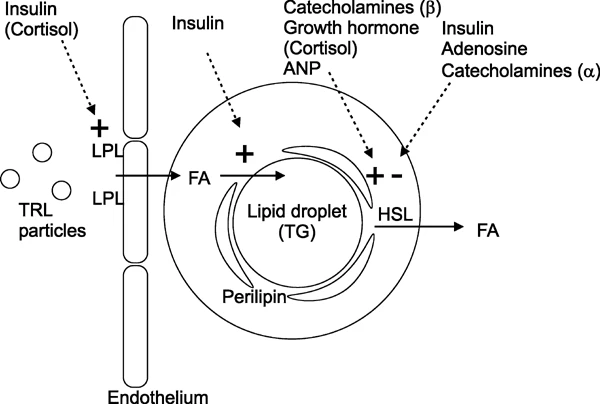
\includegraphics[width=1\linewidth]{data/chapter1/figures/adipocyte} \caption{Diagram of adipocyte fat deposition and mobilisation}\label{fig:adipocyte}
\end{figure}
\noindent
\bsmall
\emph{Figure \ref{fig:adipocyte}, reproduced from Frayn et al. (2003)\textsuperscript{\protect\hyperlink{ref-Frayn2003}{48}}, depicts influences on adipocytes that result in fat storage. Stimuli such as insulin result in positive (+) fat deposition, while other stimuli such as cortisol may result in positive or negative (-) fat deposition depending on the location of the adipocyte within the body. ANP, atrial natriuretic peptide, FA, fatty acids; LPL, lipoprotein lipase; TG, triglyceride; TRL, TG-rich lipoproteins.}
\esmall

\hypertarget{insulation}{%
\subsection{Insulation}\label{insulation}}

Energy storage of fats is managed predominantly by white adipose tissue. These deposits are located mainly within subcutaneous tissue. During infancy, brown adipose tissue is abundant; however, as humans age these deposits \emph{whiten} leaving few adult brown fat deposits. The remaining deposits of brown adipose tissue in adults are located around the neck, thoracic section of the spine, aortic body, and adrenal glands; all locations with high blood flow\textsuperscript{\protect\hyperlink{ref-Luo2016}{50},\protect\hyperlink{ref-Cannon2004}{56}}. Thermogenesis by these tissues is regulated by the hypothalamus and is achieved by uncoupling of the respiratory chain of oxidative phosphorylation via UCP1 (uncoupling protein 1). When this process is active, lipids and glucose are used as fuel\textsuperscript{\protect\hyperlink{ref-Cannon2004}{56}}. Due to the abundant vascularization of areas where brown adipose tissue is located the heat generated from this process is quickly distributed via the circulatory system. In addition, white adipose tissue can undergo a \emph{beiging} process taking on thermogenic properties of brown adipose tissue. Beige adipose tissue is a half way point between white and brown adipose tissue and is more widely dispersed than brown adipose tissue, being located mainly within subcutaneous white adipose tissue. Beige adipose tissue, much like brown adipose tissue, is cold activated but can be recruited through signalling that mimics the stressed state induced by cold. The \emph{beiging} process is not well characterized but is thought to be a result of signalling changes during differentiation of preadipocytes\textsuperscript{\protect\hyperlink{ref-Luo2016}{50}}. The \emph{beiging} process is reversible but has been suggested as a therapeutic avenue for weight loss\textsuperscript{\protect\hyperlink{ref-Cannon2004}{56}}.

\hypertarget{signalling}{%
\subsection{Signalling}\label{signalling}}

It is important to consider adipose tissue as an organ in its own right. Not solely comprised of adipocytes, adipose tissue includes a multitude of tissues and cells including connective and nerve tissues and immune cells. All respond to, and secrete, signalling molecules locally and systemically. It is thought this signalling is primarily to maintain appropriate energy stores and includes signals influencing deposition and mobilisation of fats and differentiation of new adipocytes\textsuperscript{\protect\hyperlink{ref-Frayn2003}{48},\protect\hyperlink{ref-Luo2016}{50},\protect\hyperlink{ref-Kershaw2004}{51}}. Functionally, signalling molecules have metabolic effects and/or are involved in steroid hormone production\textsuperscript{\protect\hyperlink{ref-Kershaw2004}{51}}.

Adipogenesis, the process of adipocyte formation, has been well characterized and PPAR\(y\) (peroxisome proliferator-activated receptor \(y\)) is the master regulator\textsuperscript{\protect\hyperlink{ref-Frayn2003}{48},\protect\hyperlink{ref-Luo2016}{50}}. Over-expression of PPAR\(y\) leads to differentiation and under-expression results in lipodystrophy. Other signalling molecules such as KLFs (Kruppel-like factors) and C/EBPs (CCAAT-enhancer-binding proteins) influence adipogenesis through PPAR\(y\)\textsuperscript{\protect\hyperlink{ref-Luo2016}{50}}. Because of the master regulatory function of PPAR\(y\), exploring regulatory function and expression has been considered as a potential therapeutic avenue for obesity\textsuperscript{\protect\hyperlink{ref-Luo2016}{50},\protect\hyperlink{ref-Lee2014}{57}}. Though not well characterized, brown adipocytes are thought be influenced heavily by PRDM16 and PGC1\(a\), with the latter required for thermogenesis and not necessarily adipogenesis\textsuperscript{\protect\hyperlink{ref-Luo2016}{50}}. The breakdown of stored triglycerides via lipolysis results in the release of fatty acids and glycerol molecules for oxidation and gluconeogenesis respectively. Fatty acids can also be broken down into ketone bodies via ketogenesis. While insulin abundance activates lipogenesis, the relative absence of insulin promotes lipogenesis. The lipolytic pathway, which is also activated by cAMP-dependent (cyclic adenosine monophosphate) PKA (protein kinase A), relies on the function of ATGL (adipocyte triglyceride lipase) and HSL (hormone sensitive lipase) to catalyse the hydrolysis of triglycerides to di- and mono-glyceride's respectively. Inhibition of ATGL can result in impaired lipolysis and obesity\textsuperscript{\protect\hyperlink{ref-Schreiber2019}{58}}.

The signalling molecules adipocytes produce, known as adipokines, are numerous and act on the auto- and endo-crine systems\textsuperscript{\protect\hyperlink{ref-Lehr2012}{59},\protect\hyperlink{ref-Fasshauer2015}{60}}. There are adipose deposit specific effects on expression and secretion of adipokines and the movement these adipokines can be expected to undertake. Subcutaneous adipose tissue adipokines travel through the systemic system while visceral adipose tissue adipokines can travel via the portal system with direct access to the liver. Adipocyte receptors are also expressed differentially based on deposit location\textsuperscript{\protect\hyperlink{ref-Kershaw2004}{51}}. The main adipokines (Figure \ref{fig:adipokines}) produced by adipocytes are leptin and adiponectin which function to regulate metabolism and inflammation systemically. Other cells within the adipose tissue, including immune and endothelial cells, produce much of the other adipokines such as TNF\(a\) (tumour necrosis factor \(a\)) and IL6 (interleukin 6)\textsuperscript{\protect\hyperlink{ref-Luo2016}{50}}.

Abnormal levels of adipokines are harmful, as they lead to impaired adipose tissue function and subsequent downstream effects such as insulin resistance\textsuperscript{\protect\hyperlink{ref-Luo2016}{50},\protect\hyperlink{ref-Fasshauer2015}{60}--\protect\hyperlink{ref-Bluher2015}{62}}. As adipose tissue abundance increases so too does the likelihood of abnormal levels of adipokines. This is of particular interest as adipokine levels can change as a result of diseases such as obesity, thus introducing feed-back loops which serve to alter normal processes\textsuperscript{\protect\hyperlink{ref-Fasshauer2015}{60},\protect\hyperlink{ref-Bluher2013}{61}}. However, there are outstanding questions about how abnormal levels of adipokines leads to the development of disease\textsuperscript{\protect\hyperlink{ref-Fasshauer2015}{60}}. For detailed discussion of adipokines and the pathways that lead to their production, which is not in the scope of this thesis, see\textsuperscript{\protect\hyperlink{ref-Luo2016}{50},\protect\hyperlink{ref-Kershaw2004}{51},\protect\hyperlink{ref-Fasshauer2015}{60}--\protect\hyperlink{ref-Bluher2015}{62}}.

\par
\begin{figure}
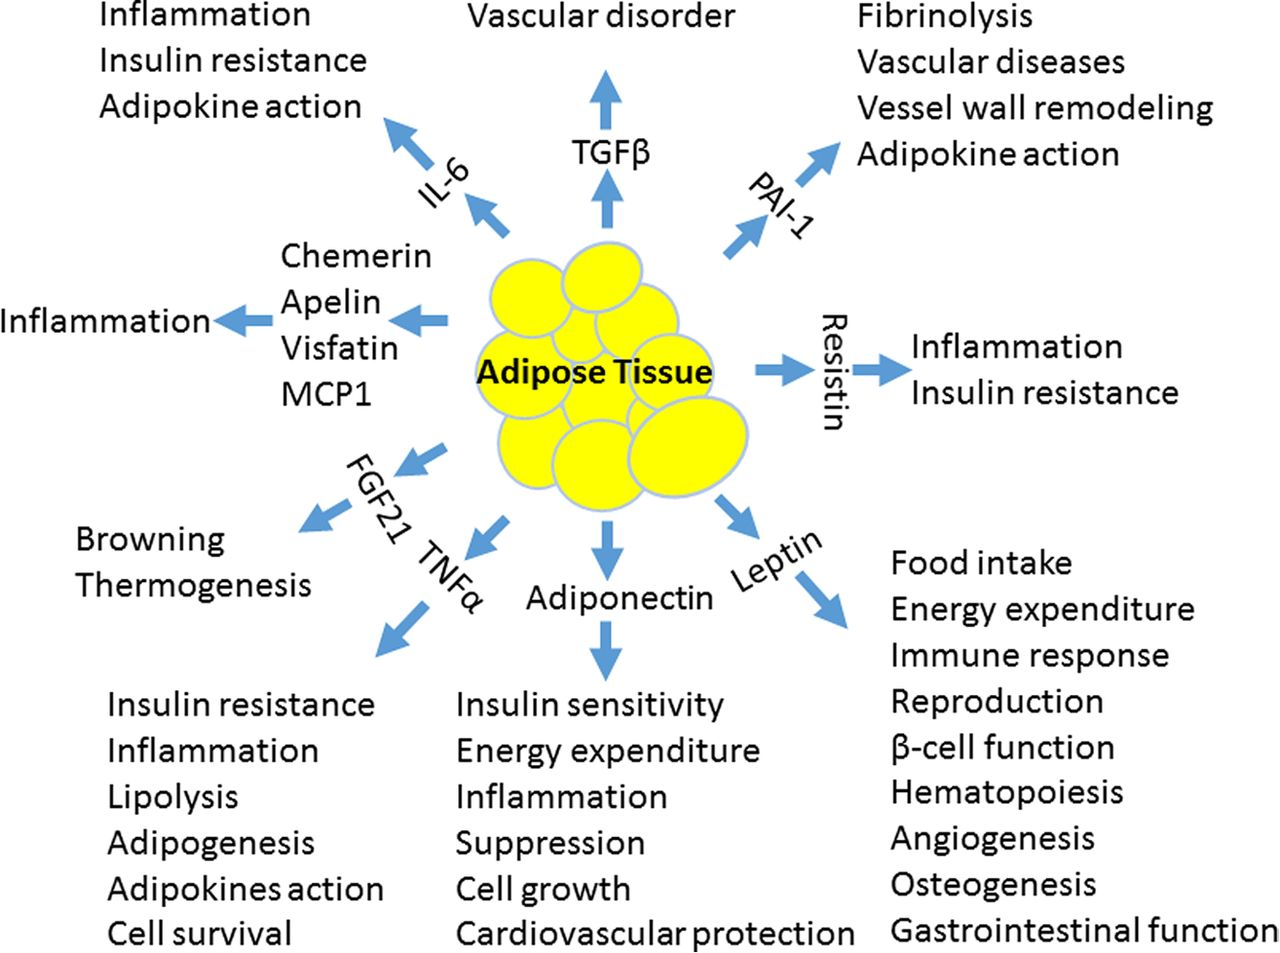
\includegraphics[width=1\linewidth]{data/chapter1/figures/adipokines} \caption{Diagram of the main adipokines secreted by adipose tiusse}\label{fig:adipokines}
\end{figure}
\noindent
\bsmall
\emph{Figure \ref{fig:adipokines}, reproduced from Luo and Liu (2016)\textsuperscript{\protect\hyperlink{ref-Luo2016}{50}}, shows the main adipokines secreted by adipose tissue and their local and systemic functions. ASP, acylating simulation protein; FGF21, fibroblast growth factor 21; IL6, interleukin 6; MCP1, monocyte chemoattractant protein 1; PAI1, plasminogen activator inhibitor 1; TNF\(a\), tumour necrosis factor alpha.}
\esmall

\hypertarget{genetics}{%
\subsection{Genetics}\label{genetics}}

Production of adipokines, though partly a response of afferent signalling, is also a result of adipocyte genetics. This is also the case for lipogenesis, storage capacity, lipolysis, mobilisation of fat deposits and energy expenditure\textsuperscript{\protect\hyperlink{ref-Dahlman2010}{52}}. A number of adipose specific genes have been identified including \emph{LEP}\textsuperscript{\protect\hyperlink{ref-Pan2018}{63},\protect\hyperlink{ref-Ahn2019}{64}}, \emph{ADIPOQ}\textsuperscript{\protect\hyperlink{ref-Achari2017}{65}}, and \emph{PPAR\(y\)}\textsuperscript{\protect\hyperlink{ref-Ahn2019}{64},\protect\hyperlink{ref-Lefterova2009}{66}} encoding the adipokines leptin and adiponectin and the adipose-specific transcription factor PPAR\(y\). These, and other genes\textsuperscript{\protect\hyperlink{ref-Ahn2019}{64}}, are expressed differently in subcutaneous and visceral adipose tissue as well as in non-adipose tissue\textsuperscript{\protect\hyperlink{ref-Ahn2019}{64}}. Differential expression along with the presence of adipose-specific genes is associated with obesity and related diseases\textsuperscript{\protect\hyperlink{ref-Ahn2019}{64}}. For example, \emph{SLC19A3} is an adipose-specific gene\textsuperscript{\protect\hyperlink{ref-Ahn2019}{64}} encoding a thiamine transporter; thiamine dependent enzymes have been associated with obesity\textsuperscript{\protect\hyperlink{ref-Maguire2018}{67}}. As adipocyte expandability is limited, and given that an excess of fatty acids results in increased adipogenesis\textsuperscript{\protect\hyperlink{ref-Frayn2003}{48},\protect\hyperlink{ref-Gray2007}{55}}, it is possible that expandability is fixed by adipose-specific genes and expression. This may have an impact on the development of diseases such as type-2 diabetes where incidence differs between different ancestral populations with the same BMI\textsuperscript{\protect\hyperlink{ref-Ma2013a}{68}}.

\hypertarget{BMI-and-disease}{%
\section{Body mass index and disease}\label{BMI-and-disease}}

With obesity responsible for 8\% of premature deaths per-year\textsuperscript{\protect\hyperlink{ref-Stanaway2018}{2}} and more people expected to be overweight or obese in the coming years\textsuperscript{\protect\hyperlink{ref-Ng2014}{3}--\protect\hyperlink{ref-Abarca-Gomez2017}{5}} it is important to understand how increased adiposity leads to mortality. Large scaleliterature searching (see Supplementary @ref(\#chapter1-appendix)) highlights the broad array of diseases and complications linking BMI and mortality. These diseases and complications can broadly be categorised as: Cancer, Cardiovascular, immune, Kidney, Liver, Neurological/behavioural, Other, Pregnancy, Respiratory, where \emph{other} includes disease like diabetes and the metabolic syndrome (Table \ref{tab:chapter1-table-MELODI}).

\hypertarget{chapter1-underlying-aetiology}{%
\section{Underlying aetiology of the BMI disease relationship}\label{chapter1-underlying-aetiology}}

Although associated with many of the same diseases, the underlying aetiology of the relationships between BMI, WHR and BF with these diseases is not clear. For quality of life, the relationship is mostly explained by the presence of co-morbidities which increases the likelihood of poor outcomes. Stigmatisation as a result of increased fat mass may also be involved in poor quality of life\textsuperscript{\protect\hyperlink{ref-Bray2004}{69},\protect\hyperlink{ref-Haslam2005}{70}}. Similarly, the relationship with many sleep complications is likely a result of chronic pulmonary diseases -- distribution of fat mass around the neck may also be important\textsuperscript{\protect\hyperlink{ref-Bray2004}{69}--\protect\hyperlink{ref-Poulain2006}{71}}.

Type 2 diabete development is likely to follow a process of impaired glucose clearance as a result of increased adiposity, which leads to increased insulin resistance. There are likely wider metabolic changes that influence this process which are also a consequence of increased adiposity\textsuperscript{\protect\hyperlink{ref-Collaboration2009}{23},\protect\hyperlink{ref-Bray2004}{69},\protect\hyperlink{ref-Haslam2005}{70}}. Respiratory diseases are likely a result of reductions in FEV1, FVC, lung and residual capacity, and expiratory reserve. Each of these is a consequence of weakened muscles and reduced compliance of the chest which can be caused by the physical burden of increased adiposity around the chest and lungs\textsuperscript{\protect\hyperlink{ref-Haslam2005}{70},\protect\hyperlink{ref-Poulain2006}{71}}. With respiratory disease there is also the prospect of confounding as a result of smoking status, which increases with increased adiposity\textsuperscript{\protect\hyperlink{ref-Carreras-Torres2018}{72}}. In the case of cardiovascular disease, hypertension may be related to changes in: sympathetic activity, blood flow and viscosity, and dietary intake as a result of increased adiposity\textsuperscript{\protect\hyperlink{ref-Bray2004}{69},\protect\hyperlink{ref-Haslam2005}{70},\protect\hyperlink{ref-Jayedi2018}{73}}. Some of these changes might similarly be a result of metabolic, inflammatory and hormonal changes. Both dyslipidemia and reductions in HDL result from increased adiposity and these changes may be important in development of heart disease.

Unlike diabetes and respiratory diseases, most other diseases have a less well understood process of development as a result of increased adiposity. Increased adiposity is associated with numerous types of cancer. Hypotheses for these associations differ based on the type of cancer. Metabolic, inflammatory and hormonal changes as a result of increased adiposity are proposed as leading to the development of a number of different cancers\textsuperscript{\protect\hyperlink{ref-Collaboration2009}{23},\protect\hyperlink{ref-Bray2004}{69},\protect\hyperlink{ref-Haslam2005}{70},\protect\hyperlink{ref-Bhaskaran2014}{74}}.

The location of fat deposits may also be important (e.g.~deposition of adipose tissue around the heart may result in inflammation of the myocardium, but this might also be subsequent to dyslipidemia and reduction in HDL\textsuperscript{\protect\hyperlink{ref-Collaboration2009}{23},\protect\hyperlink{ref-Bray2004}{69},\protect\hyperlink{ref-Haslam2005}{70},\protect\hyperlink{ref-Dagfinn2016}{75}}). Osteoarthritis, though likely a result of the physical burden of increased adiposity, may also be a product of changes to cartilage and bone metabolism\textsuperscript{\protect\hyperlink{ref-Bray2004}{69},\protect\hyperlink{ref-Haslam2005}{70}}. Similar metabolic changes may play a role in a number of other diseases. An increased risk of gallstones is associated with increased cholesterol\textsuperscript{\protect\hyperlink{ref-Bray2004}{69}} and increased salt intake has been suggested as a potential link between increased adiposity and stroke\textsuperscript{\protect\hyperlink{ref-Collaboration2009}{23},\protect\hyperlink{ref-Haslam2005}{70}}.

The body of work investigating associations between increased adiposity and disease is extensive. Many proposed mechanisms of disease development invovle the physical burden of fat mass and/or changes to different pathways, particularly metabolic changes. However, the potential for residual confounding and reverse causation in these studies warrants further investigation using methods robust to there challenges.

\hypertarget{mendelian-randomization}{%
\section{Mendelian randomization}\label{mendelian-randomization}}

Studies investigating the associations between increased adiposity and metabolites and metabolites and disease are important and, when conducted in optimal conditions provide information on the potential causes and consequences of altered metabolic states. Even with optimal conditions observational studies hold a number of limitations that can not easily be overcome. These limitations, such as confounding and reverse causation, can lead to biased results\textsuperscript{\protect\hyperlink{ref-DaveySmith2014}{76}--\protect\hyperlink{ref-Yarmolinsky2018}{79}}. Simply put, though a study may identify an association between two traits does not mean that one causes the other; they may be correlated because of shared causes for instance.

In observational epidemiology, ideally we want to compare individuals based on the exposure and so attempt to control the experiment by accounting for confounderis. In this regard we attempt to replicate a randomised control trial, wich is the gold standard for testing causality. However, the large costs and time required to develop, implement and analyse results limits their use. More importantly, randomizing individuals to conditions known to be associated with harmful outcomes is ethically wrong. An alternative approach is to utilise the large amounts of data that are publicly available or that can be accessed through institutions. Causal inference methodologies have been established to exploit the availability of these data sets.

Mendelian randomization (MR), described\textsuperscript{\protect\hyperlink{ref-DaveySmith2003}{80},\protect\hyperlink{ref-DaveySmith2003}{80},\protect\hyperlink{ref-Davies2018}{81}} and reviewed\textsuperscript{\protect\hyperlink{ref-Burgess2015}{82},\protect\hyperlink{ref-Bowden2019}{83}} elsewhere, and accompanied by a \href{https://doi.org/10.31219/osf.io/6yzs7}{dictionary} of terms\textsuperscript{\protect\hyperlink{ref-Lawlor2019}{84}}, is a statistical methodology that uses genetic variants as instrumental variables to investigate the causal relationship between an exposure and outcome\textsuperscript{\protect\hyperlink{ref-DaveySmith2003}{80},\protect\hyperlink{ref-Smith2004}{85}}. The reassessment of many observational associations has provided strong evidence for the relationships between risk factors and diseases, but has also highlighted the biases and limitations of observational research\textsuperscript{\protect\hyperlink{ref-Timpson2005}{77}--\protect\hyperlink{ref-Yarmolinsky2018}{79}}.

Briefly, individuals inherit alleles largely at random from their mother and father. Across a large population this leads to the even distribution of confounders between the effect and non-effect alleles. As such, individuals differ because of the expressed allele rather than their environmental circumstances. This random allocation of genetic variants, which may ultimately be related to a health outcome, is analogous to a randomised control trial where geneotype groups act as the intervention and non-intervention arms of the trial.

Inference derived from MR analyses relies up-on three assumptions (Figure \ref{fig:chapter1-figure-mr-dag}): (i) the instrumental variable (\(Z\)) is robustly associated with the exposure (\(X\)), (ii) there is no independent association of the instrumental variable with the outcome (\(Y\)) other than through the exposure, (iii) the instrumental variable is independent of measured or un-measured confounders (\(U\)).
\begin{figure}
\includegraphics[width=1\linewidth]{thesis_files/figure-latex/chapter1-figure-mr-dag-1} \caption{Directed acyclic graph of the Mendelian randomization principle}\label{fig:chapter1-figure-mr-dag}
\end{figure}
\noindent
\bsmall
\emph{\(Z\) = instrumental variable; \(X\) = exposure; \(Y\) = outcome; \(U\) = confounders.}
\esmall

Additional assumptons based on homogeneity, monotonicity, and effect modification are also present. The homogeneity assumption assumes the assoication between the IV and the is exposure or the effect of the exposure on the outcome is homogeneous. That is, the association or the effect is the same for all individuals in the population. Monotonicity can be deterministic or stochastic. Deterministic monotonicity assumes that the effect of the IV is consistent in all individuals of the population. That is, the effect of the IV does not increase the exposure in one group and decrease it in another. Stochastic monotonicity assumes deterministic monotonicity conditional on confounders.

Based up-on Mendel's laws of inheritance, MR relies on the assumption that genetic variants are unlikely to be associated with one another (outside of linkage disequilibrium) or with environmental factors. Deviation from which would mean an uneven distribution of alleles across a population. Consideration in MR analyses should therefore also be given to dynastic effects, population structure, and assortative mating. Within family MR can be used to obtain the true causal effect in these situations\textsuperscript{\protect\hyperlink{ref-Hartwig2018}{86},\protect\hyperlink{ref-Brumpton2019}{87}}.

Dynastic effects, a form of confounding, are a consequence of traits transmitted across generations which then influence the causal effect estimate\textsuperscript{\protect\hyperlink{ref-Brumpton2019}{87},\protect\hyperlink{ref-Sanderson2019}{88}}. That is, the parental genotype directly effects the offspring phenotype. For example, the effect BMI on cardiovascular disease may be biased by the instrumental variables for BMI being correlated across parent and offspring and the effect of maternal BMI on offspring development, which has an effect on future cardiovascular disease. In this instance the seond MR assumption would be violated. Within family studies are proposed, and simulations have shown, to overcome some of the consequences of dynastci effects\textsuperscript{\protect\hyperlink{ref-Brumpton2019}{87},\protect\hyperlink{ref-Sanderson2019}{88}}.

Population structure is a result of allele frequency differning across geographic regions. This would violate the assumption that instrumental variables are independent of confounding factors. In MR analyses it is assumed that latent structure is accounted for in the genome-wide association study (GWAS) in which the instrumental variables are discovered\textsuperscript{\protect\hyperlink{ref-Haworth2019}{89}}. As the sample sizes of GWAS's has increased the potential for subtle effects of population structure has been observed\textsuperscript{\protect\hyperlink{ref-Haworth2019}{89},\protect\hyperlink{ref-Berg2019}{90}}.

Assortative mating is the principle by which partners select one another based on a particular phenotype. This is either cross-trait (one trait selecting for another trait) or single-trait (one trait selecting for the same trait). MR results can be biased by both types of assortative mating, even when the phenotypes of interest are not those which influenced the mating\textsuperscript{\protect\hyperlink{ref-Hartwig2018}{86}}.

Canalization, whereby what would otherwise be developmentally deleterious genetic effects are nullified by compensatory mechanisms, is broadly equivalent to non-adherence in an RCT. Any effects of canalization would attenuate effect sizes\textsuperscript{\protect\hyperlink{ref-Smith2004}{85}}, however there are currently no methods to detect its presence in an MR context. The effects of canalization are unlikely to be present in MR studies which utilise maternal genotypes for environmental exposures of the offspring such as during gestation\textsuperscript{\protect\hyperlink{ref-Smith2010}{91}}. For complex traits it is possible that canalization occurs at the level of the system rather than at the gene level\textsuperscript{\protect\hyperlink{ref-Geiler-Samerotte2019}{92}}. As such, any outcome of a genetic mutation in regards to its role in the canal would likely be unpredictable.

Methodological advances have enabled MR studies to be conducted with both individual level, known as one-sample MR, and summary level data obtained from published GWASs\textsuperscript{\protect\hyperlink{ref-Pierce2013}{93}}, known as two-sample MR. In both contexts, instrumental variables are often obtained from external GWAS's. Increasingly, these are large and well powered GWAS' able to idnetify ever increasing numbers of SNPs associatied with complex traits such as with BMI\textsuperscript{\protect\hyperlink{ref-Speliotes2010a}{94}--\protect\hyperlink{ref-Yengo2018}{98}}. As power has increased, the ability to detect SNPs with smaller effects and which explain ever smaller proportions of variance in BMI has increased\textsuperscript{\protect\hyperlink{ref-Yengo2018}{98}}. This holds potential considerations in regards to population structure and the effects of an omnigenic model.

As discussed, population structure was thought to have been an issue in smaller studies and could be accounted for by adjustment. However, well powered studies have shown both latent structure\textsuperscript{\protect\hyperlink{ref-Haworth2019}{89},\protect\hyperlink{ref-Berg2019}{90}} and an inability to perform adequate adjustemnt\textsuperscript{\protect\hyperlink{ref-Sohail2019}{99}}. This has potential implications, not only for the effect sizes of associated SNPs but also for the identification of SNPs associated with the trait\textsuperscript{\protect\hyperlink{ref-Sohail2019}{99}}. For example, a poorly or un-adjusted GWAS could identify SNPs associated with population differences rather than the trait of interest.

In an omnigenic model, variance in a trait of interest is not solely a result of directly related genes (core-genes). Rather, all genes expressed in relevant cell types have an effect, however small, on the trait of interest\textsuperscript{\protect\hyperlink{ref-Boyle2017}{100}}. These peripheral-genes, which have no obvious direct link to the trait of interest, are mostly in non-coding regions with regulatory functions\textsuperscript{\protect\hyperlink{ref-Liu2019}{101}}.Given that variants associated with complex traits are dispersed widely across the genome\textsuperscript{\protect\hyperlink{ref-Liu2019}{101}} and that assigning a link between any particular SNP and an individual gene is difficult\textsuperscript{\protect\hyperlink{ref-GTEx2013}{102}}, variants associated with complex traits likely implicate many genes with the trait. Because many of these will be peripheral-genes they will ultimately have functions on other traits, which in an MR context may include the outcome and thus violate the exclusion restriction assumption.

Additional considerations include random measurement error (random measurmeent in the exposure will bias towards the null, and increase the standard error if in the outcome), Winners curse (whereby discovery studies identify larger effects than those in replication studies), collider bias (conditioning on a variable by adjustment, restriction, or sampling can induce an association betwene \(X\) and \(Y\) biasing th estimate both away and towards the null), non-overlapping samples (specific to two-sample MR, where the exposure and outcome data are obtained from samples with shared individuals), horizontal pleiotropy (the instrumental variable has an affect on the outcome independent of the exposure), and vertical pleiotropy (the instrumental variable does not have an effect on the exposure directly but on traits that have an effect on the exposure).

Among the considerations and limitations of MR, population stratification, horizontal pleiotropy and canalization are the most challenging to account for. Though one can restrict analyses to homogeneous groups, use principal components, and perform within family studies to examine and mitigate the effects of population stratification, biases (e.g.~sampling bias) may still remain. Additionally, methods for assessing potential horizontal pleiotropy exist but formal assessment of the exclusion restriction assumption is not possible. Accounting for canalization is much harder and, though being aware of the underlying biology can inform ones analyses, methods for assessment do not exist. Unlike the other considerations, vertical pleiotropy does not necessarily bias MR results rather it highlights potential intermediates.

Both one-sample and two-sample MR can be extended to investigate intermediates that sit on the causal pathway. Mediation analysis in MR is discussed in detail elsewhere\textsuperscript{\protect\hyperlink{ref-Carter2020}{103}} and can be achieved using two-step\textsuperscript{\protect\hyperlink{ref-Relton2012}{104}}/network MR\textsuperscript{\protect\hyperlink{ref-Burgess2015b}{105}} and multivariable MR\textsuperscript{\protect\hyperlink{ref-Sanderson2018}{106}} (MVMR). Briefly, mediation analysis is interested in identifying the total effetc, the direct effect, and the indirect effect; where all act in the same direction the proportion of the total effect explained by teh mediator (proportion mediated) can be calculated\textsuperscript{\protect\hyperlink{ref-VanderWeele2016}{107}}. The total effect is the effect of the exposure on the outcome through all mediated pathways, the direct effect is the effect of the exposure on the outcome through all mediated pathways that are not the pathway of interest, the indirect effect is the effect of the exposure on the outcome through the mediator of interest. These analyses are predicated on the following assumptions: (i) that there is a causal effect of the exposure on the outcome and mediator and of the mediator on the outcome; (ii) that there is no confounding between exposure, mediator, and outcome; (iii) that there are no intermediate confounders; (iv) that there is no interaction between the exposure and mediator\textsuperscript{\protect\hyperlink{ref-VanderWeele2016}{107}}.

In two-step MR (Figure \ref{fig:chapter1-figure-mr-dag2}) the indirect effect is calculated by multiplying the effect of the exposure on the mediator and the effect of the mediator on the outcome. The three core MR assumptions (and all previous considerations) must still be met and also extended: (i) the instrumental variables (\(Z\) \& \(Z2\)) must be robustly associated with the exposure or intermediate only (\(X\) and \(M\)), (ii) the instrumental variables for the exposure (\(Z\)) must not be associated with the intermediate (\(M\)) or the outcome (\(Z\)) other than through the exposure (\(X\)), and the intermediate instrumental variables (\(Z2\)) must not be associated with the exposure, and only with the outcome (\(Y\)) through the intermediate, (iii) the instrumental variables for the exposure and intermediate must not be associated with measured or unmeasured confounders. No interaction between exposure and mediator is also assumed. Two-step MR has been used\textsuperscript{\protect\hyperlink{ref-Varbo2015}{108}--\protect\hyperlink{ref-Marouli2019}{110}} and combined with MVMR\textsuperscript{\protect\hyperlink{ref-Carter2019}{111}} to gain better insight into disease aetiology.
\begin{figure}
\includegraphics[width=1\linewidth]{thesis_files/figure-latex/chapter1-figure-mr-dag2-1} \caption{Directed acyclic graph of the two-step Mendelian randomization principle}\label{fig:chapter1-figure-mr-dag2}
\end{figure}
\noindent
\bsmall
\emph{\(Z\) = instrumental variable; \(X\) = exposure; \(M\) = intermediate; \(U\) = confounders; \(Z2\) = instrumental variable for \(M\); \(Y\) = outcome.}
\esmall

Multivariable MR allows for the causal effects of multiple exposures on an outcome to be estimated\textsuperscript{\protect\hyperlink{ref-Sanderson2018}{106}} (Figure \ref{fig:chapter1-figure-mr-dag3}). The effect of each exposure is estimated conditional on the other exposures and thus provides a direct estimate of the effect. Figure \ref{fig:chapter1-figure-mr-dag3} shows a simplified MVMR model with two exposures (\(X\) and \(X2\)); the bidirectional line between exposure one and exposure two does not make an assumption about the exposure relationships. The indirect effect is estimated by subtraction of the direct effect from the total effect. The total effect is calculated using univariable MR. As with two-step MR, no interaction between exposure and mediator is assumed. Though a new approach, and still subject to the same assuptions as with two-step and univariable MR, MVMR has shown promise in elucidating underlying aetiology of complex traits\textsuperscript{\protect\hyperlink{ref-Carter2019}{111}--\protect\hyperlink{ref-Johnson2019}{114}}.
\begin{figure}
\includegraphics[width=1\linewidth]{thesis_files/figure-latex/chapter1-figure-mr-dag3-1} \caption{Directed acyclic graph of the multivariable Mendelian randomization principle using two exposures}\label{fig:chapter1-figure-mr-dag3}
\end{figure}
\noindent
\bsmall
\emph{\(Z\) = instrumental variables associated with one or more of the exposures; \(X\) = exposure; \(X2\) = second exposure; \(Y\) = outcome.}
\esmall

Though two-step MR was devised with epigenetic mechanisms in mind\textsuperscript{\protect\hyperlink{ref-Relton2012}{104}} and MVMR has shown promise investigating metabolic intermediates\textsuperscript{\protect\hyperlink{ref-Richardson2019}{113}}, their application to large omic data sets is yet to be shown. An alternative approach, which insted of estimating mediated effects looks for overlapping signals, may also be appropriate for omic data{[}NOTE: INSERT REF TO RCC PAPER{]}. In this regard, the effect of the exposure on the candidate intermediate and the effect of candidate intermediate on the outcome are ranked in terms of their effects. A candidate intermediate is considered to be a potential mediator if it ranks highly in both analyses. {[}NOTE: DISUCSS LIMITATIONS ONCE PAPER IS COMPLETED{]}

\hypertarget{metabolites}{%
\section{Metabolites}\label{metabolites}}

Many of the diseases discussed (Section \ref{chapter1-underlying-aetiology}) have hypothesised development processes involving metabolic, inflammatory and hormonal changes. As a complex signalling organ with both local and systemic effects, adipose tissue is likely to influence all three of these processes at both local and systemic levels. It is not within the scope of this thesis to investigate all three, but recent advances in measurement methodologies and the availability of large, and deeply phenotyped population based studies may now provide the data necessary to investigate metabolic effects.

The metabolome, the total abundance of small-molecules, is a reflection of genetic and non-genetic factors and sits between the proteome and the phenotype\textsuperscript{\protect\hyperlink{ref-Griffin2006}{115}--\protect\hyperlink{ref-Wishart2019}{118}}. The metabolome can be separated into endogenous (internally produced) and exogneous (externally produced) metabolites, whereby the majority of metabolites are the result of cellular processes, with multiple functions including as energy, signalling, transportattion, and structural components. Metabolic effects can be far reaching and also include post-translational modifications\textsuperscript{\protect\hyperlink{ref-Wishart2019}{118},\protect\hyperlink{ref-Johnson2016}{119}}. During homeostasis metabolic effects are tightly controlled, however the many functions they play mean that imbalances can be detrimental\textsuperscript{\protect\hyperlink{ref-Griffin2006}{115},\protect\hyperlink{ref-Wishart2019}{118},\protect\hyperlink{ref-Johnson2016}{119}}.

Measurement of individual metabolites, at scale, is achieved predominantly through mass spectrometry (MS) and nuclear magnetic resonance (NMR). Both MS and NMR have differing limitations with full coverage of the metabolome not achieved by either. Complimentary usage of the two methods is desirable\textsuperscript{\protect\hyperlink{ref-Fearnley2016}{120}}; however, as MS is destructive and both methods are costly this is not always possible. Many population-based studies have metabolomics data from only one measurement method limiting the number of metabolites available for analysis.

The number, and type, of metabolites identified by MS and NMR methods is dependent upon whether a targeted, semi-targeted, or un-targeted approach is taken. Targeted metabolomics analysis uses an internal standard to characterize individual metabolites\textsuperscript{\protect\hyperlink{ref-Roberts2012}{121},\protect\hyperlink{ref-Liu2017b}{122}} whereas un-targeted metabolomics analysis measures all metabolites within a specified range\textsuperscript{\protect\hyperlink{ref-Liu2017b}{122},\protect\hyperlink{ref-Vinayavekhin2010}{123}}. Semi-targeted approaches use internal standards to quantify groups of metabolites with similar chemical structure\textsuperscript{\protect\hyperlink{ref-Liu2017b}{122}}. Targeted studies are able to identify a handful of metabolites where as semi-targeted and un-targeted can identify hundreds to thousands. As targeted and semi-targeted methods use internal standards absolute quantification of metabolit abundance is possible. In un-targeted methods only relative quantification, the peak area of each metabolite in comparison to other samples, is possible\textsuperscript{\protect\hyperlink{ref-Liu2017b}{122}}.

The availability of well powered population studies with metabolomics data from targeted, semi-targeted, and un-targeted methods as well as matched genome-wide data has enabled a growth in metaboloite GWASs\textsuperscript{\protect\hyperlink{ref-Chu2019}{117},\protect\hyperlink{ref-Fearnley2016}{120}}. These studies have revealed large variations in the heritability of metabolites and numerous loci associated with their abundances{[}\protect\hyperlink{ref-Shin2014}{124}; \protect\hyperlink{ref-Kettunen2016}{125}; \protect\hyperlink{ref-Long2017}{126}; \protect\hyperlink{ref-Gallois2019}{127}; Lotta2020{]}. The public availability of these GWASs provides a unique opportunity to perform genetic epidemiology studies which can compliment the existing literature from observational association studies.

Metabolites reflect the current condition and activity of an organism and vary in abundance depending on the state of the individual. This is particularly evident in fasted and non-fasted measurements\textsuperscript{\protect\hyperlink{ref-Carayol2015}{128}--\protect\hyperlink{ref-Teruya2019}{130}} but also in case control studies such as those focussing on diabetes\textsuperscript{\protect\hyperlink{ref-Guasch-Ferre2016}{131}} and cancer\textsuperscript{\protect\hyperlink{ref-Johnson2016}{119},\protect\hyperlink{ref-Liesenfeld2013}{132}}. Differences are also apparent when studying complex traits such as BMI\textsuperscript{\protect\hyperlink{ref-Moore2014}{133},\protect\hyperlink{ref-Cirulli2019}{134}} as well as many more\textsuperscript{\protect\hyperlink{ref-Wishart2018}{135}} - a searchable database of metabolite information, including links with disease, is available from \href{hmdb.ca}{The Human Metabolome Database}.

These studies provide an overall assessment of the changes metabolites undergo as a result of different conditions but the relationship is not clear. Whether metabolites change as a result of a condition or lead to its development is an important question with potential clinical importance. Mutable, both from a genetic and non-genetic perspective, the metabolome can, with caution, be used to investigate the development of diseases\textsuperscript{\protect\hyperlink{ref-Su2014}{116},\protect\hyperlink{ref-Chu2019}{117},\protect\hyperlink{ref-Fearnley2016}{120}}. Particular consideration should be given to the metabolomics approach (targeted, semi-targeted, untargeted) and whether individuals were fasted. Consideration should also be given to the fact that metabolomics analysis provides a snapshot of an individuals current state. Though few studies have investigated metabolomic stability in large populations, variability in metabolite measures is apparent\textsuperscript{\protect\hyperlink{ref-Carayol2015}{128},\protect\hyperlink{ref-Sampson2013}{136},\protect\hyperlink{ref-Darst2019}{137}}.

A key aspect of future work investigating relationships between metabolites and diseases are the interactions metabolites have with one another. The metabolome is a complex system involving feedback and feed-forward loops, this complexity means many metabolites are intercorrelated\textsuperscript{\protect\hyperlink{ref-Rosato2018}{138}}, have high genetic correlation\textsuperscript{\protect\hyperlink{ref-Gallois2019}{127}} and share a common genetic architecture\textsuperscript{\protect\hyperlink{ref-Shin2014}{124}--\protect\hyperlink{ref-Gallois2019}{127},\protect\hyperlink{ref-Lotta2020}{139}}. As such, a perturbation in a single metabolite rarely occurs in isolation. Investigating metabolites as grouped entities that represent the underlying complexity, rather than individual metabolites, may help to elucidate relationships with disease.

\newpage

\hypertarget{aims}{%
\section{Aims}\label{aims}}

Increased adiposity is a global health concern. Many of the consequence of increased adiposity are known but the underlying aetiology is not well understood. Adipose tissue is a prolific signalling organ with systemic effects some of which are likely to affect the metabolome. Individual metabolites have been associated with many diseases but the complexity of the network makes these analyses difficult. MR studies provide an opportunity to investigate and disentangle the complex relationship between exposure, intermediate and outcome. These studies must be approached carefully given the interrelatedness of metabolites. In light of these considerations this thesis aims to:
\begin{itemize}
\tightlist
\item
  \emph{Identify metabolites that sit on the causal pathway from increased adiposity to disease}
\end{itemize}
\hypertarget{objectives}{%
\subsection{Objectives}\label{objectives}}

In order to achieve this aim this thesis will investigate the following objectives:
\begin{enumerate}
\def\labelenumi{\arabic{enumi}.}
\tightlist
\item
  Perform a systematic review (Chapter \ref{chapter2}) of all MR studies in which a measure of increased adiposity was used as an exposure. The diseases identified in this work will guide the diseases investigated (Chapter \ref{chapter9}). 
\end{enumerate}
\par
\begin{enumerate}
\def\labelenumi{\arabic{enumi}.}
\setcounter{enumi}{1}
\tightlist
\item
  Identify and describe appropriate instrumentation of increased adiposity. The systematic review (Chapter \ref{chapter2}) will provide information on current instrumentation practices for MR. I will use this information and test MR instrument assumptions using individual level data to select instruments for subsequent analyses (Chapters \ref{chapter3} and \ref{chapter4}). 
\end{enumerate}
\par
\begin{enumerate}
\def\labelenumi{\arabic{enumi}.}
\setcounter{enumi}{2}
\tightlist
\item
  Identify metabolites associated with increased adiposity in observational (Chapter \ref{chapter4}) and MR settings (Chapter \ref{chapter5}).
\end{enumerate}
\par
\begin{enumerate}
\def\labelenumi{\arabic{enumi}.}
\setcounter{enumi}{3}
\tightlist
\item
  Gain overview of metabolic profiles to enable interpretation of analyses from Chapters \ref{chapter4}, \ref{chapter5}, and \ref{chapter9} using visualisation tools (Chapter \ref{chapter6}). 
\end{enumerate}
\par
\begin{enumerate}
\def\labelenumi{\arabic{enumi}.}
\setcounter{enumi}{3}
\tightlist
\item
  Implement methods to reduce the complexity of the metabolome and produce instruments for MR analyses (Chapters \ref{chapter7} and \ref{chapter8}). 
\end{enumerate}
\par
\begin{enumerate}
\def\labelenumi{\arabic{enumi}.}
\setcounter{enumi}{4}
\tightlist
\item
  Identify diseases associated with metabolites in an MR setting (Chapter \ref{chapter9}) and present the investigated network of increased adiposity -\textgreater{} metabolites -\textgreater{} diseases. 
\end{enumerate}
\newpage

\hypertarget{summary}{%
\section{Summary}\label{summary}}

Within this chapter I have\ldots{}\ldots{}{[}NOTE: look to kaitlins thesis for an idea of how to link chapters together{]}

\hypertarget{presentation-of-results}{%
\section{Presentation of results}\label{presentation-of-results}}

In this thesis large association analyses are conducted. The presentation and interpretation of this data is complicated by the highly inter-correlated nature of metabolomics data and the need to compare effects across multiple exposures, models and ages. To this effect, and discussed in detail in Chapter \ref{chapter6}, Circos plots have been used to visualise results. To aid interpretation of these going forward, and unless otherwise stated in the figure legend, the following applies:
\begin{itemize}
\tightlist
\item
  Each point represents a single test of an exposure on an outcome
\item
  Labels around the edge of the plot represent outcomes
\item
  Tracks represent a single variable (e.g.~an exposure)
\item
  Each point is accompanied by a 95\% confidence interval
\item
  Solid points represent a multiple testing threshold has been reached
\item
  Data is split into sections (denoted by numbers) which is dictated by grouping outcomes by a variable (e.g.~subclass)
\end{itemize}
\hypertarget{chapter2}{%
\chapter{Systematic review}\label{chapter2}}

\textbf{TITLE OF CHAPTER}

\hypertarget{chapter3}{%
\chapter{Instrumentation}\label{chapter3}}

\hypertarget{instrumenting-measures-of-increased-adiposity}{%
\section*{\texorpdfstring{\emph{Instrumenting measures of increased adiposity}}{Instrumenting measures of increased adiposity}}\label{instrumenting-measures-of-increased-adiposity}}
\addcontentsline{toc}{section}{\emph{Instrumenting measures of increased adiposity}}

Although the prevailing thought is that BMI, WHR, and BF\% are all highly correlated there is little recent evidence from studies investigating all three measures simultaneously in the same populations. Evidence mainly comes from a study by Pouliot et al. (1994)\textsuperscript{\protect\hyperlink{ref-Pouliot1994}{140}}; for men they found corrleatins of: BMI and BF\% = 0.85, BMI and WHR = 0.78, WHR and BF\% = 0.70; women: BMI and BF\% = 0.96, BMI and WHR = 0.58, WHR and BF\% = 0.55. See Chapter \ref{chapter3}

Given the high correlation between BMI, WHR, and BF\% (at least sex specifically in the case of WHR and BF\% - See Chapter \ref{chapter3}) it may be likely that a study reporting an association between BMI and a disease will also show a similar association with WHR and/or BF\%. We looked for review articles for BMI and multiple diseases and looked for studies reporting BMI and WHR and/or BF\% to identify if studies found similar associations across multiple measures of increased adipsoity. Table \ref{tab:literature-associations} shows studies identifying an association between BMI and a disease and studies which show similar associations with WHR and BF\%. A summary of the studies which discuss underlying aetiology of the associations is also presented.

As a result, we first set out to investigate the correlation between BMI, WHR, and BF\% in two independent population based studies: the Avon Longitudinal Study of Parents and Children\textsuperscript{\protect\hyperlink{ref-Fraser2013}{141},\protect\hyperlink{ref-Boyd2013}{142}}(ALSPAC) and UK Biobank\textsuperscript{\protect\hyperlink{ref-Collins2012}{143}--\protect\hyperlink{ref-Sudlow2015}{145}}.

\hypertarget{correlation-of-measures-of-increased-adiposity}{%
\subsection{Correlation of measures of increased adiposity}\label{correlation-of-measures-of-increased-adiposity}}

\hypertarget{data}{%
\subsubsection{Data}\label{data}}

The Avon Longitudinal Study of Parents and Children (ALSPAC) is a large prospective cohort study that recruited 14,541 pregnancies in the former Avon Health Authority area in South West England, with expected delivery dates between the 1st April 1991 and the 31st December 1992\textsuperscript{\protect\hyperlink{ref-Fraser2013}{141},\protect\hyperlink{ref-Boyd2013}{142}} (See \protect\hyperlink{supp-alspac}{Supplementary Information, ALSPAC Overview}, for full details). We used data from the Focus clinics for mothers and fathers. We used the clinic with the highest response rate for each of mothers and fathers, this was clinic 1 for both. For Focus on Mothers 1 (FOM1) data was collected between December 2008 and July 2011 with a total of 4,832 women attending clinic. Because mother may have enrolled multiple pregnancies the total number of cases in the release data is 4,978 mothers; the mean age of the mothers was 47.89 (4.497 SD). For Focus on Fathers 1 (FOF1) data was collected between September 2001 and February 2013 and a total of 2,001 fathers attended the clinic. Multiple pregnanices resulted in a total number of cases in the release data as 2,034; the mean age of fathers was 53.3 (5.427 SD). Prior to data analysis we removed duplicate cases of mothers and fathers using \texttt{R}\textsuperscript{\protect\hyperlink{ref-r2019}{146}}(version 3.5.3) resulting in 4,831 and 2,001 women and men for analysis.

In FOM1 and FOF1 BMI was derived from \texttt{weight\ (kg)\ /\ height\ (m\^{}2\^{})}; WHR was derived from \texttt{wasit\ circumference\ (cm)\ /\ hip\ circumference\ (cm)}; BF\% was obtained from a full-body scan using a narrow fan beam dual-emission X-ray absorptiometry (DXA; Lunar Prodigy) scanner and derived from \texttt{total\ fat\ mass\ /\ (total\ fat\ free\ mass\ +\ total\ fat\ mass)\ *\ 100}. Data was avaliable on 4,632 women and 1,826 men (Table \ref{tab:study-characteristics}).

UK Biobank is a prospective study of \textasciitilde{}500,000 individuals aged 37-79 recruited from 2006-2010 who were registered with the Natonal Health Service in the United Kingdom and lived close to one of 22 assessment centres. Participants provided a range of information at a single assessment (See \protect\hyperlink{supp-biobank}{Supplementary Information, UK Biobank Overview})\textsuperscript{\protect\hyperlink{ref-Collins2012}{143}--\protect\hyperlink{ref-Sudlow2015}{145}}. We used the final release of data () which included information on XXX women and XXX men. Before analysis we removed all individuals\ldots{}\ldots{} this resulted in XXX and XXX women and men for analysis.

In UK Biobank BMI was derived from \texttt{weight\ (kg)\ /\ height\ (m\^{}2\^{})}; WHR was derived from \texttt{wasit\ circumference\ (cm)\ /\ hip\ circumference\ (cm)}; BF\% was obtained \ldots{}\ldots{}\ldots{}\ldots{}\ldots{}\ldots{}\ldots{}\ldots{}. Data was avaliable on 4,632 women and 1,826 men (Table \ref{tab:study-characteristics}).
\begin{longtable}[t]{ccccc}
\caption{\label{tab:study-characteristics}Study characteristics for measures of increased adiposity in ALSPAC and UK Biobank.}\\
\toprule
\multicolumn{1}{c}{ } & \multicolumn{2}{c}{ALSPAC} & \multicolumn{2}{c}{UK Biobank} \\
\cmidrule(l{3pt}r{3pt}){2-3} \cmidrule(l{3pt}r{3pt}){4-5}
 & Women & Men & Women & Men\\
\midrule
BMI & 4810 & 1976 & 1 & 1\\
WHR & 4809 & 1985 & 2 & 2\\
BF\% & 4649 & 1839 & 3 & 3\\
Total & 4632 & 1826 & 4 & 4\\
\bottomrule
\end{longtable}
\noindent
\emph{Table \ref{tab:study-characteristics} shows the number of individuals from the Avon Longitudinal Study of Parents and Children (ALSPAC) and UK Biobank with available data for each measure of increased adiposity after removing individuals with missing data for each trait. Total shows the number of individuals with a measure for all three measures of increased adiposity; we performed correlation analysis on this group. BMI = body mass idnex; WHR = waist hip ratio; BF\% = body fat percent; Total = the number of individuals for each category with inforation on all three measures and after exclusions.}

\hypertarget{statistical-analysis}{%
\subsubsection{Statistical analysis}\label{statistical-analysis}}

To investigate the correlation between BMI, WHR, and BF\% we performed a Pearson's product-moment correlation in \texttt{R}\textsuperscript{\protect\hyperlink{ref-r2019}{146}}(version 3.5.3) for each of ALSPAC women, men, sex combined, and UK Biobank women, men, and sex combined. All results are reported in Table \ref{tab:correlation-results} and shown in Figure \ref{fig:correlation-results-figure-alspac} and \ref{fig:correlation-results-figure-ukbiobank}.
\begin{longtable}[t]{ccccccc}
\caption{\label{tab:correlation-results}Correlation results for measures of increased adiposity in ALSPAC and UK Biobank.}\\
\toprule
\multicolumn{1}{c}{ } & \multicolumn{2}{c}{Women} & \multicolumn{2}{c}{Men} & \multicolumn{2}{c}{Combined} \\
\cmidrule(l{3pt}r{3pt}){2-3} \cmidrule(l{3pt}r{3pt}){4-5} \cmidrule(l{3pt}r{3pt}){6-7}
 & R & CI & R & CI & R & CI\\
\midrule
\addlinespace[0.3em]
\multicolumn{7}{l}{\textbf{ALSPAC}}\\
\hspace{1em}BMI \& WHR & 0.48 & 0.46 -- 0.50 & 0.63 & 0.60 -- 0.66 & 0.42 & 0.40 -- 0.44\\
\hspace{1em}BMI \& BF\% & 0.81 & 0.80 -- 0.82 & 0.77 & 0.75 -- 0.79 & 0.65 & 0.63 -- 0.66\\
\hspace{1em}WHR \& BF\% & 0.36 & 0.33 -- 0.38 & 0.65 & 0.63 -- 0.68 & -0.09 & -0.06 -- -0.11\\
\addlinespace[0.3em]
\multicolumn{7}{l}{\textbf{UK Biobank}}\\
\hspace{1em}\hspace{1em}BMI \& WHR & 1.00 & 1 & 1.00 & 1 & 1.00 & 1\\
\hspace{1em}\hspace{1em}BMI \& BF\% & 2.00 & 2 & 2.00 & 2 & 2.00 & 2\\
\hspace{1em}\hspace{1em}WHR \& BF\% & 3.00 & 3 & 3.00 & 3 & 3.00 & 3\\
\bottomrule
\end{longtable}
\emph{Table \ref{tab:correlation-results} shows the Pearson's product-moment correlation estimates (R) and associated 95\% confidence interval (CI) for each combination of BMI, WHR, and BF\% seperated by sex and data source. Combined = sex combined analysis; ALSPAC = Avon Longitudinal Study of Parents and Children; R = Pearson's product-moment correaltion estimate; CI = 95\% confidence interval for the correlation estimate. All correlation results reporte a p-value \textless{} 2.2 x 10\textsuperscript{-16} except for: ALSPAC sex combined WHR \& BF\% (p-value = 5.197 x 10\textsuperscript{-12}),\ldots{}\ldots{}\ldots{}\ldots{}\ldots{}\ldots{} }
\noindent
\begin{figure}
\includegraphics[width=1\linewidth]{data/chapter3/figures/correlation_alspac} \caption{Scater plots of ALSPAC individuals data on measures of increased adiposity}\label{fig:correlation-results-figure-alspac}
\end{figure}
\emph{Figure \ref{fig:correlation-results-figure-alspac} shows scatter plots for ALSPAC women (top), men (middle) and combined (bottom) data on BMI and WHR (left), BMI and BF\% (centre), and WHR and BF\% (right). A linear model line with 95\% confidence interval is shown along with the Pearson's product-moment correalation (R) and associated 95\% confidence intervals (95\% CI) and p-values at the top of each scatter. BMI = body mass idnex; WHR = waist hip ratio; BF\% = body fat percent. All correlation results report a p-value \textless{} 2.2 x 10\textsuperscript{-16} except for ALSPAC sex combined WHR \& BF\% (p-value = 5.197 x 10\textsuperscript{-12}).}
\noindent
\bigskip
\bigskip

\emph{Figure \ref{fig:correlation-results-figure-ukbiobank} shows scatter plots for UK Biobank women (top), men (middle) and combined (bottom) data on BMI and WHR (left), BMI and BF\% (centre), and WHR and BF\% (right). A linear model line with 95\% confidence interval is shown along with the Pearson's product-moment correalation (R) and associated 95\% confidence intervals (95\% CI) and p-values at the top of each scatter. BMI = body mass idnex; WHR = waist hip ratio; BF\% = body fat percent. All correlation results report a p-value\ldots{}\ldots{}\ldots{}\ldots{}\ldots{}\ldots{}.}
\noindent
\bigskip
\bigskip

In ALSPAC our results show the highest correlations between BMI and BF\% for both men (95\% CI = 0.75 -- 0.79) and women (95\% CI = 0.80 -- 0.82), with similarly high correaltion for sex combined (95\% CI = 0.63 -- 0.66).

Our measure of DXA derived measure of BF\% in ALSPAC is likely a more accurate quantification of BF\% than Pouliot et al. (1994)\textsuperscript{\protect\hyperlink{ref-Pouliot1994}{140}} who derived BF\% using hydrostatic weighing and an estimation equation\textsuperscript{\protect\hyperlink{ref-SIRI1956}{147}}. Differences in estimates from ALSPAC and Pouliot et al. (1994)\textsuperscript{\protect\hyperlink{ref-Pouliot1994}{140}} may also be a result of sample sizes with only 70 women and 81 men in Pouliot et al. (1994)\textsuperscript{\protect\hyperlink{ref-Pouliot1994}{140}}, with 66 and 22.5 times more women and men available for analysis in ALSPAC.

For UK Biobank correlation estimates are\ldots{}\ldots{}\ldots{}.. .

ALSPAC
men women combined
BMI and WHR = 0.60-0.66 0.46-0.50 0.40-0.44
BMI and BF\% = 0.75-0.79 0.80-0.82 0.63-0.66
WHR and BF\% = 0.63-0.68 0.33-0.38 -0.06- -0.11

UK Biobank
men women combined
BMI and WHR =\\
BMI and BF\% =
WHR and BF\% =

Pouliot et al. (1994)\textsuperscript{\protect\hyperlink{ref-Pouliot1994}{140}}
men women
BMI and BF\% = 0.85 0.96
BMI and WHR = 0.78 0.58
WHR and BF\% = 0.70 0.55

\hypertarget{supplementary-information}{%
\section{Supplementary Information}\label{supplementary-information}}

\hypertarget{supp-alspac}{%
\subsection{ALSPAC Overview}\label{supp-alspac}}

Pregnant women resident in Avon, UK with expected dates of delivery 1st April 1991 to 31st December 1992 were invited to take part in the study. The initial number of pregnancies enrolled is 14,541 (for these at least one questionnaire has been returned or a ``Children in Focus'' clinic had been attended by 19/07/99). Of these initial pregnancies, there was a total of 14,676 foetuses, resulting in 14,062 live births and 13,988 children who were alive at 1 year of age. When the oldest children were approximately 7 years of age, an attempt was made to bolster the initial sample with eligible cases who had failed to join the study originally. As a result, when considering variables collected from the age of seven onwards (and potentially abstracted from obstetric notes) there are data available for more than the 14,541 pregnancies mentioned above. The number of new pregnancies not in the initial sample (known as Phase I enrolment) that are currently represented on the built files and reflecting enrolment status at the age of 24 is 913 (456, 262 and 195 recruited during Phases II, III and IV respectively), resulting in an additional 913 children being enrolled. The phases of enrolment are described in more detail in the cohort profile paper and its update (see footnote 4 below). The total sample size for analyses using any data collected after the age of seven is therefore 15,454 pregnancies, resulting in 15,589 foetuses. Of these 14,901 were alive at 1 year of age. A 10\% sample of the ALSPAC cohort, known as the Children in Focus (CiF) group, attended clinics at the University of Bristol at various time intervals between 4 to 61 months of age. The CiF group were chosen at random from the last 6 months of ALSPAC births (1432 families attended at least one clinic). Excluded were those mothers who had moved out of the area or were lost to follow-up, and those partaking in another study of infant development in Avon.

The study website \url{http://www.bristol.ac.uk/alspac/} contains details of all the data that is available through a fully searchable data dictionary and variable search tool \url{http://www.bristol.ac.uk/alspac/researchers/our-data/}. Ethical approval for the study was obtained from the ALSPAC Ethics and Law Committee and the Local Research Ethics Committees \url{http://www.bristol.ac.uk/alspac/researchers/research-ethics/}. Informed consent for the use of data collected via questionnaire and clinics was obtained from participants following recommendations of the ALSPAC Ethics and Law Committee at the time. Full details of the ALSPAC consent procedures are available on the study website \url{http://www.bristol.ac.uk/alspac/researchers/research-ethics/}.

\hypertarget{supp-biobank}{%
\subsection{UK Biobank Overview}\label{supp-biobank}}

This research has been conducted using the UK Biobank Resource under \emph{Application Number 16391}.

\hypertarget{chapter4}{%
\chapter{Observational analysis}\label{chapter4}}

\hypertarget{associations-between-measures-of-adiposity-and-metabolites-observational-analysis}{%
\subsubsection{\texorpdfstring{\emph{Associations between measures of adiposity and metabolites: observational analysis}}{Associations between measures of adiposity and metabolites: observational analysis}}\label{associations-between-measures-of-adiposity-and-metabolites-observational-analysis}}

In Chapters \protect\hyperlink{chapter1}{1} and \protect\hyperlink{chapter2}{2}, the link between increased adiposity and disease was presented both in observational and causal analysis frameworks. This work highlighted key limiting areas in understanding the biological pathways leading to disease development. In this chapter, observational epidemiological methods will be used to assess one of the potential pathways linking adiposity to disease, metabolites. The aim of this chapter is to provide an observational grounding for subsequent causal analysis work in Chapters \protect\hyperlink{chapter5}{5} and \protect\hyperlink{chapter9}{9}.

\newpage

\hypertarget{introduction}{%
\section{Introduction}\label{introduction}}

In Chapter \protect\hyperlink{chapter1}{1} and \protect\hyperlink{chapter2}{2}, a growing body of work both observational and causal was presented linking increased adiposity to many diseases. Many of these, and others, have proposed metabolites to be involved in this process\textsuperscript{\protect\hyperlink{ref-Collaboration2009}{23},\protect\hyperlink{ref-Bray2004}{69},\protect\hyperlink{ref-Haslam2005}{70}}. However, few studies have identified intermediate metabolites and pathways that lie on the disease development pathway.

Metabolic changes as a result of increased adiposity have recently been highlighted in a systematic review\textsuperscript{\protect\hyperlink{ref-Rangel-Huerta2019}{148}}. The studies included reveal the wide scale metabolic change as a result of obesity. However, the majority of studies included fewer than 100 individuals and all focused on obesity as a singular measure of adiposity.

Analysis across thousands of individuals has highlighted the wide range of global effects BMI has on the metabolome\textsuperscript{\protect\hyperlink{ref-Wurtz2014}{149}}. To our knowledge, the work by Wurtz et al. (2014)\textsuperscript{\protect\hyperlink{ref-Wurtz2014}{149}} is the largest investigation of the effects of increased adiposity on the metabolome to date. Their analysis, involving 88 metabolites measured in 12,664 adolescents and young adults, identified a majority of metabolites to be associated with increased BMI after adjusting for sex. Associations were observed across numerous metabolic classes including amino acids, fatty acids, hormones, inflammatory markers, and lipids. Amino acids were positively associated with BMI, with the largest effect observed for phenylalanine. Fatty acids showed similarly positive effects, except for n-6 fatty acids percentage and polyunsaturated fatty acids percentage which showed negative associations. A positive association was observed for LDL metabolites while a heterogeneous pattern of association was found for HDL metabolites. In MR analysis, similar results were found.

Given the crude estimation of adiposity provided by BMI, the effects identified by Wurtz et al. (2014)\textsuperscript{\protect\hyperlink{ref-Wurtz2014}{149}} require further consideration across a number of measures of adiposity. The Avon Longitudinal Study of Parents and Children (ALSPAC), a longitudinal birth cohort study, provides an opportunity to expand on this work using data from many thousands of individuals with multiple measures of adiposity and metabolomics data measured at multiple time points. Here, observational analysis of measures of adiposity and metabolites provide a basis from which to investigate causal associations. In addition, replication of results from Wurtz et al.\textsuperscript{\protect\hyperlink{ref-Wurtz2014}{149}} is possible for a number of metabolites.

\newpage

\hypertarget{methods}{%
\section{Methods}\label{methods}}

Data were available for exposures (measures of adiposity), outcomes (metabolites), and potential confounders from the Avon Longitudinal Study of Parents and Children (ALSPAC). In ALSPAC, exposures included body mass index (BMI), waist hip ratio (WHR) and body fat percentage (BF); metabolomics data was available for up to 234 metabolites, which included metabolite ratios; data on available confounders included: age, sex, mothers or own education, smoking history, alcohol history, diet, physical activity. All analysis and data manipulation was performed using \texttt{R} (version 3.6.2)\textsuperscript{\protect\hyperlink{ref-r2019}{146}}. Specific \texttt{R} packages are described where appropriate. All code for this work is available on \href{https://github.com/mattlee821/000_thesis/index/data/chapter4}{GitHub}.

\hypertarget{overview-alspac}{%
\subsection{Overview: ALSPAC}\label{overview-alspac}}

ALSPAC\textsuperscript{\protect\hyperlink{ref-Fraser2013}{141},\protect\hyperlink{ref-Boyd2013}{142},\protect\hyperlink{ref-Northstone2019}{150}} is a large prospective cohort study that invited women resident in Avon, UK with expected dates of delivery between 1st April 1991 and 31st December 1992 to participate. The initial number of pregnancies enrolled was 14,541 (for these at least one questionnaire has been returned or a ``Children in Focus'' clinic has been attended by 19/07/99). Of these initial pregnancies, a total of 14,676 fetuses, resulted in 14,062 live births and 13,988 children alive at one year of age.

When the oldest children were approximately seven years of age, an attempt was made to bolster the initial sample with eligible cases who had failed to join the study originally. As a result, when considering variables collected from the age of seven onwards (and potentially abstracted from obstetric notes) there are data available for more than the 14,541 pregnancies mentioned above. The number of new pregnancies not in the initial sample (known as Phase I enrollment) that are currently represented on the built files and reflecting enrollment status at the age of 24 is 913 (456, 262 and 195 recruited during Phases II, III and IV respectively), resulting in an additional 913 children being enrolled. The phases of enrollment are described in more detail in the cohort profile paper and its update\textsuperscript{\protect\hyperlink{ref-Fraser2013}{141},\protect\hyperlink{ref-Boyd2013}{142},\protect\hyperlink{ref-Northstone2019}{150}}. The total sample size for analyses using any data collected after the age of seven is therefore 15,454 pregnancies, resulting in 15,589 fetuses, of which 14,901 were alive at one year of age.

The study \href{http://www.bristol.ac.uk/alspac/}{website} contains details of all the data that is available through a fully searchable data dictionary and \href{http://www.bristol.ac.uk/alspac/researchers/our-data/}{variable search tool}. Ethical approval for the study was obtained from the ALSPAC Ethics and Law Committee and the \href{http://www.bristol.ac.uk/alspac/researchers/research-ethics/}{Local Research Ethics Committees}. Informed consent for the use of data collected via questionnaire and clinics was obtained from participants following recommendations of the ALSPAC Ethics and Law Committee at the time. Full details of the ALSPAC consent procedures are available on the \href{http://www.bristol.ac.uk/alspac/researchers/research-ethics/}{study website}.

ALSPAC data is split by clinic visits. For this work, data for children was taken from the following clinics: Focus at 7 (\textasciitilde{}7 years old), Focus at 8 (\textasciitilde{}8 years old), Before Breakfast Study (\textasciitilde{}8 years old), Teen Focus 3 (\textasciitilde{}15 years old) Teen Focus 4 (\textasciitilde{}17 years old), Focus at 24 (\textasciitilde{}24 years old). Data on adults was taken from: Focus on Mothers 1 (\textasciitilde{}50 years old), Focus on Mothers 2 (\textasciitilde{}50 years old), and Focus on Fathers 1 (\textasciitilde{}50 years old). The Before Breakfast Study only collected metabolomics data, as such data on exposures and confounders were extracted for these individuals from the Focus at 8 clinic. Metabolomics data for each time point were extracted first and subsequent data on exposures and confounders were extracted for individuals with metabolomics data.

\hypertarget{outcomes-metabolites}{%
\subsection{Outcomes: metabolites}\label{outcomes-metabolites}}

There were slight differences in the methodology used across time points for the children and for the fathers metabolomics measurements. However, data are directly comparable (See the metabolomics data release file D5700 from the ALSPAC Data Dictionary). Briefly, high-throughput proton (\textsuperscript{1}H) nuclear magnetic resonance (NMR) assays were performed on EDTA plasma/serum samples. Samples were predominantly fasted. Measurements were taken at three molecular windows (lipoprotein lipids, low molecular-weight metabolites, and lipid extracts) enabling broad quantification of over 220 metabolomic measures. Full details on the NMR methodology has previously been described\textsuperscript{\protect\hyperlink{ref-Soininen2009}{151}--\protect\hyperlink{ref-Soininen2015}{154}} and is available from the \href{http://www.bristol.ac.uk/alspac/researchers/access/}{ALSPAC data dictionary} (data dictionary identifiers: children = D5704, mothers = D5705, fathers = D5700). The Before Breakfast study does not have a documentation file and is described elsewhere\textsuperscript{\protect\hyperlink{ref-Ong2004}{155}}. Descriptions of metabolites are available in the Appendix \ref{chapter4-appendix-metabolites}.

The spectral NMR data was processed by Nightingale Health and provided as a processed file with identifiable individuals (triplets/quadruplets) and individuals who had withdrawn consent removed. Some mothers and fathers were duplicated in the raw data due to the way in which mothers were originally enrolled into the study and assigned IDs. If a mother enrolled with two different pregnancies (both having an expected delivery date within the recruitment period (April 1991-December 1992)), she will have two separate IDs. A father associated with both of these pregnancies will also be duplicated. Duplicate measurements for mothers and fathers were removed. Raw metabolomics data was therefore available for: Focus at 7 (n = 5518; metabolites = 230), Before Breakfast Study (n = 640; metabolites = 228), Teen Focus 3 (n = 3371; metabolites = 230), Teen Focus 4 (n = 3175; metabolites = 230), Focus at 24 (n = 3269; metabolites = 224), Focus on Mothers 1 (n = 4362; metabolites = 230), Focus on Mothers 2 (n = 2708; metabolites = 230), Focus on Fathers (n = 1833; metabolites = 230).

In order to maximize the sample size at each clinic, data were combined where clinics were within a similar age range. For these combined data sets, duplicate individuals (i.e.~those attending both clinics) were identified, and the measurement from the most recent clinic was dropped. The number of metabolites measured at each clinic visit for the children and adult data differed; unique metabolites were included in the combined data set. Raw, combined, metabolomics data was therefore available for: children (mean age (SD) = 7.56 (0.36); n = 5656; metabolites = 234), adolescents (mean age (SD) = 16.06 (1.11); n = 4489; metabolites = 230), young adults (mean age (SD) = 24.03 (0.85); n = 3269; metabolites = 224), adults (mean age (SD) = 49.53 (5.32)n = 6406; metabolites = 232; Table \ref{tab:chapter4-table-ALSPAC-N}).

Quality control of the combined metabolite data (i.e.~children, adolescents, young adults, adults) was performed using the \texttt{R} package \href{https://github.com/MRCIEU/MetaboQC}{\texttt{MetaboQC}} (version 0.0.1). Quality control was performed twice, firstly including and secondly excluding the derived metabolomics measures from missingness and clustering. Briefly, individuals, and then metabolites, with high missingness (\textgreater{}=80\%) were removed. Missingness was then re-calculated for individuals and metabolites, with removal based on 20\% missingness. Individuals were then removed based on total sum abundance, considering outliers as \textgreater{} 5 standard deviations away from the mean. Using this metabolite data set, a dendrogram based on a Spearman's rho distance matrix is produced, and a set of clusters identified based on a Spearman's rho of 0.5. For each cluster, the metabolite with the least missingness is tagged as the representative feature. Finally, principal component analysis is conducted using the representative features to evaluate structure among individuals. Outliers are identified as being \textgreater{} 5 standard deviations away from the mean of principal component 1 and 2 and were excluded.

\hypertarget{exposures-measures-of-adiposity}{%
\subsection{Exposures: measures of adiposity}\label{exposures-measures-of-adiposity}}

Measures of adiposity (BMI, WHR, BF) were obtained for all individuals with available raw metabolomics data; identifiable individuals and those with withdrawn consent were therefore already excluded. As metabolomics measures were obtained on unique individuals where multiple clinics were attended, anthropometric data for these individuals were taken from the clinic associated with the metabolomic measure. No anthropometric data was available for the Before Breakfast Study, so the Focus at 8 clinic, as the most age appropriate clinic, was used instead. For this combined data, Focus at 7 measures were matched with Focus at 7 metabolomics measures and Focus at 8 measures were matched with Before Breakfast Study metabolomics measures.

Measures for children were taken from Focus at 7 and 8, for adolescents Teen Focus 3 and 4, for mothers Focus on Mothers 1 and 2, for fathers Focus on Fathers. Data on WHR was not available in adolescents. BMI was calculated as \(\displaystyle \frac{weight(kg)}{height (m^2)}\) and WHR as \(\displaystyle \frac{waist\ circumference\ (cm)} {hip\ circumference\ (cm)}\). BF was measured in adolescents, young adults, and adults using dual energy x-ray absorptiometry (DXA). Briefly, measurement required individuals to be prone and stationary while a Lunar prodigy narrow fan beam densitometer performed a whole body DXA scan. Data was processed using Lunar Prodigy software. Individuals did not have measurements taken if they: were pregnant; had a radiological investigation using contrast media within the week before the DXA scan; had a recent nuclear medicine investigation with persistent radioactivity; weighed greater than 159kg. BF was calculated as a percentage as \(\displaystyle \frac{fat\ mass} {fat\ mass + fat\ free\ mass}\ * 100\). Available anthropometric measures for individuals with metabolomics data is given in Table \ref{tab:chapter4-table-ALSPAC-adiposity} and distributions given in Figure \ref{fig:chapter4-figure-raincloudplot-adiposity-measures}.

In children, BF was not measured. A bioeletrical impedance measure was available; briefly, children were encouraged to pass urine and undress to their underclothes. A Tanita Body Fat Analyser (Model TBF 305) was used to measure weight and impedance. Height was entered to the nearest \(cm\) and `female standard' was used for all children for sex. The Tanita Body Fat Analyser TBF 305 is a single frequency (50\(kHz\)) leg-to-leg device. In single frequency devices, impedance is a representation of resistance which is related to the volume of water (which one assumes makes up the majority of fat free mass (FFM)), as such, the higher the resistance/impedance the greater the amount of FFM. Calculation of BF from the impedance measure is only possible at the time of measurement, however these derived BF measures were not stored and the equation to calculate them was not available from the manufacturer (Appendix \ref{chapter4-appendix-communications}).

Previous work\textsuperscript{\protect\hyperlink{ref-Chouinard2007}{27}} has shown that comparison of BF derived from the manufacturer's equation and an alternative\textsuperscript{\protect\hyperlink{ref-Jebb2000}{26}} showed little difference in resulting BF. The equation was derived in a study involving 205 (101 women) healthy adults with a mean age of 43.8 (SD = 16) for men and 40.4 (SD = 13.6) for women. The equation, where \(Z\) is the impedance measure from the device in \(ohms\), height is in meters, weight is in kilograms, age is in years, and female-specific components are given in parenthesis, is given as:
\begin{equation}
\begin{split}
  BF = -156.1 - 89.1\ ln(height) \\
  \ +\ 45.6\ ln(weight) \\
  \ +\ 0.120\ age\ \\
  \ +\ 0.0494\ Z \\
  \ +\ (19.6\ ln(height))
\end{split}
  \label{eq:BF}
\end{equation}
Given that the equation was derived from adult data, its application to child data was explored. A raw impedance measure, from a similar model (Tanita Body Fat Analyser (Model TBF 401A)), was obtained for adolescents and the equation was used to compare BF derived from the impedance device and BF measured with DXA in adolescents. Exploration involved visual inspection of distribution and Spearman's correlation with BMI, height, weight and other BF measures in adolescents. The same observations were carried out for raw impedance.

\hypertarget{confounders}{%
\subsection{Confounders}\label{confounders}}

Data on confounders were obtained for all individuals with raw metabolomics data; identifiable individuals and those with withdrawn consent were therefore already excluded. The following confounders were used: age, sex, maternal/own education, smoking, alcohol, diet, physical activity. Age was taken from the metabolomics clinic visit. The number of individuals with available data is given in Table \ref{tab:chapter4-table-ALSPAC-confounders}.

Maternal education was used for children, adolescents and young adults. Own education was used for mothers and mother reported partner education was used for fathers. Specifically, mothers were asked, during their pregnancy, `What educational qualifications do you, your partner, your mother, and your father have?' with possible answers: CSE or GCSE (D, E, F or G), O-level or GCSE (A, B, or C), A-level, qualifications in shorthand/ typing/or other skills, e.g.~hairdressing, apprenticeship, state enrolled nurse, state registered nurse, City and Guilds intermediate technical, City \& Guilds final technical, City \& Guilds full technical, teaching qualification, university degree, no qualification, qualifications not known, not applicable, other (please describe).

Smoking was binary; adolescents (at the metabolomics clinic), young adults (at the metabolomics clinic), and adults (mothers were asked during pregnancy; fathers were asked in 2013) were asked whether they had ever smoked a cigarette before.

Adolescents (Teen Focus 3) were asked what their alcohol drinking pattern was with possible answers: only ever tried drinking once/twice, used to drink sometimes {[}but{]} never drink now, sometimes drink but less than once a week, usually drink on 1/2 days a week, usually drink on \textgreater{}2 days a week but not every day, usually drink every day. Adolescents (Teen Focus 4), young adults (at the metabolomics clinic), mothers (in 2013), and fathers (at the metabolomics clinic) were asked the frequency they had drinks containing alcohol with possible answers: never, monthly or less, two to four times a month, two to three times a week, four or more times a week.

Diet data, as predicted kilo-calories consumed per day, was derived from Anderson et al. (2013)\textsuperscript{\protect\hyperlink{ref-Anderson2013}{156}} and avaialble for ages 7 and 13. Data from age 7 was matched with metabolomics data for children while data from age 13 was matched with adolescents. Diet data was not available for young adults or adults.

In adolescents and young adults, accelerometry data was collected at the same clinic for which metabolomics data were collected. Briefly, individuals wore an accelerometry device for the days following their clinic visit whilst keeping a diary of the times they wore and took off the device. Individuals were advised to wear the accelerometer device if the following days were part of a `normal week' with regards to their activity. For young adults, physical activity data is the average number of minutes per day spent doing moderate to vigorous physical activity. For adolescents, data was available from Teen Focus 3 and is the mean counts per minute spent doing moderate to vigorous physical activity for the whole week. Adults were asked `do you take part in physical activity (e.g.~running, swimming, dancing, golf, tennis, squash, jogging, bowls)?' with possible answers: no, occasionally (less than monthly), frequently (once a month or more). Data for mothers was available in 2010, fathers data was available at the metabolomics clinic. Physical activity data was not available for children.

\hypertarget{statistical-analysis}{%
\subsection{Statistical analysis}\label{statistical-analysis}}

To investigate the association between measures of adiposity and metabolites, all exposures were Z-scored and linear regression was performed. Variables known to influence the metabolomic profile and adiposity (age\textsuperscript{\protect\hyperlink{ref-Yu2012}{157},\protect\hyperlink{ref-Brennan2020}{158}}, sex\textsuperscript{\protect\hyperlink{ref-Brennan2020}{158}}, education\textsuperscript{\protect\hyperlink{ref-Zajacova2018}{159}}, smoking\textsuperscript{\protect\hyperlink{ref-Bonevski2014}{160}}, alcohol\textsuperscript{\protect\hyperlink{ref-Bonevski2014}{160}}, diet\textsuperscript{\protect\hyperlink{ref-Afshin2019}{161}}, and physical activity\textsuperscript{\protect\hyperlink{ref-ODonoghue2018}{162}}), were included as confounders. Three linear models were used to investigate potential effects of these confounding variables. Model 1 included age at the metabolomics clinic visit and sex. Model 2 included model 1 and mothers/own level of highest education, whether respondent had ever smoked, frequency respondent had a drink containing alcohol, and predicted kilo-calories consumed per day (diet). Model 3 comprised model 2 and physical activity. For models 1 and 2, individuals with data on all confounders except physical activity were included. Model 3 comprised all individuals included in model 1 and 2 who also had data on physical activity.

For all analyses, the units represent the absolute change in each metabolite per standard deviation change in the exposure. Ninety-five percent confidence intervals were calculated and a multiple testing threshold specific for each group was applied. Multiple testing thresholds were calculated as the number of independent metabolites within the raw data given a Spearman's rho of approximately 0.75 among the metabolites with data for at least 20\% of samples -- this was calculated during metabolite quality control. The number of independent metabolites in each group was: children = 42, adolescents = 42, young adults = 40, adults = 44.

\hypertarget{presentation}{%
\subsubsection{Presentation}\label{presentation}}

Metabolites were grouped into subclasses (grouping data provided by the metabolomics platform) based on biological pathway. Model 2, as the most adjusted and given the reduced sample size in Model 3, is presented as the main analysis for this work. Consistency in the direction of effect estimates across models within each exposure and age group was investigated, as was the number of tests reaching a multiple testing threshold. Directional consistency was investigated for exposures across age groups for model 2. A Spearmans Rho analysis was used to investigate the correlation between effect estimates across exposures and age groups. Visualization and comparison of global metabolic profiles across exposures within age groups, and within exposures and across age groups was performed using Circos plots using the \texttt{EpiViz} \texttt{R} package{[}{]}. Forestplots, created using the \texttt{ggforestplot} \texttt{R} package, were used to examine specific subclasses where variation among metabolites within the subclass and strong effects were identified. Results for derived measures and \emph{Lipoprotein particle size} and \emph{Fatty acid ratios} are presented in the supplement. Effect estimates were compared to that of previous work by Wurtz et al. (2014)\textsuperscript{\protect\hyperlink{ref-Wurtz2014}{149}}.

\newpage

\hypertarget{results}{%
\section{Results}\label{results}}

In total, metabolomics data was available for 234 metabolites in children (N = 5656), 230 metabolites in adolescents (N = 4489), 224 metabolites in young adults (N = 3269), and 232 metabolites in adults (N = 6406; Table \ref{tab:chapter4-table-ALSPAC-N}). Quality control was performed twice, firstly including derived metabolites and secondly excluding them. There was a large difference in the number of representative features identified across the two runs, as such quality controlled data used here on was produced having included derived metabolites.

Quality control resulted in: 6 individuals and 4 metabolites removed from the children's data (4 samples excluded for \textgreater{}= 80\% missingness; 1 sample excluded for total sum abundance \textgreater{}= 5 SD from the mean; 1 sample excluded as a result of being \textgreater{}= 5 SD from the mean of PC1 and 2; 4 metabolites removed for \textgreater{}= 20\% missingness), 5 individuals and 0 metabolites removed from the adolescents data (1 sample excluded for total sum abundance \textgreater{}= 5 SD from the mean; 4 samples excluded as a result of being \textgreater{}= 5 SD from the mean of PC1 and 2), 4 individuals and 0 metabolites removed from the young adults data (1 sample excluded for total sum abundance \textgreater{}= 5 SD from the mean; 3 sample excluded as a result of being \textgreater{}= 5 SD from the mean of PC1 and 2), 7 individuals and 4 metabolites removed from the adults data (1 sample excluded for total sum abundance \textgreater{}= 5 SD from the mean; 6 samples excluded as a eresult of being \textgreater{}= 5 SD from the mean of PC1 and 2; 4 metabolites removed for \textgreater{}= 20\% missingness). Quality controlled metabolomics data available for analysis is given in Table \ref{tab:chapter4-table-ALSPAC-QC-N}. A total of 220 metabolites were measured in all age groups. Of individuals with metabolomics data, a majority also had data on measures of adiposity (Table \ref{tab:chapter4-table-ALSPAC-adiposity} and Figure \ref{fig:chapter4-figure-raincloudplot-adiposity-measures}), except for adolescents where data on WHR was not available. Data on confounders were also available in the majority of individuals, the exception being phsyical activity where much fewer individuals had available data and no data was available for children (Table \ref{tab:chapter4-table-ALSPAC-adiposity}.

\blandscape
\begin{table}

\caption{\label{tab:chapter4-table-ALSPAC-N}Metabolomics data available in ALSPAC}
\centering
\begin{tabular}[t]{lrrlrlrl}
\toprule
Combined group & N & N
 metabolites & Subgroup & Subgroup
N & Unique
N & Total
metabolites & Unique
metabolites\\
\midrule
 &  &  & 7 & 5518 & 5016 & 230 & 5\\
\cmidrule{4-8}
\multirow{-2}{*}{\raggedright\arraybackslash Children} & \multirow{-2}{*}{\raggedleft\arraybackslash 5656} & \multirow{-2}{*}{\raggedleft\arraybackslash 234} & 8 & 640 & 138 & 228 & 7\\
\cmidrule{1-8}
 &  &  & 15 & 3371 & 1314 & 230 & 0\\
\cmidrule{4-8}
\multirow{-2}{*}{\raggedright\arraybackslash Adolescents} & \multirow{-2}{*}{\raggedleft\arraybackslash 4489} & \multirow{-2}{*}{\raggedleft\arraybackslash 230} & 17 & 3175 & 1118 & 230 & 0\\
\cmidrule{1-8}
Young adults & 3269 & 224 & 24 & 3269 & -- & 224 & --\\
\cmidrule{1-8}
 &  &  & Focus on mothers 1 & 4362 & 1865 & 230 & 0\\
\cmidrule{4-8}
\multirow{-2}{*}{\raggedright\arraybackslash Mothers} & \multirow{-2}{*}{\raggedleft\arraybackslash 4573} &  & Focus on mothers 2 & 2708 & 211 & 230 & 0\\
\cmidrule{1-2}
\cmidrule{4-8}
Fathers & 1833 & \multirow{-3}{*}{\raggedleft\arraybackslash 230} & Focus on fathers & 1833 & -- & 230 & --\\
\cmidrule{1-8}
 &  &  & Mothers & 4573 & -- & 230 & 2\\
\cmidrule{4-8}
\multirow{-2}{*}{\raggedright\arraybackslash Adults} & \multirow{-2}{*}{\raggedleft\arraybackslash 6406} & \multirow{-2}{*}{\raggedleft\arraybackslash 232} & Fathers & 1833 & -- & 230 & 2\\
\bottomrule
\end{tabular}
\end{table}
\noindent 
\bsmall
\emph{Table \ref{tab:chapter4-table-ALSPAC-N}: the number of individuals with metabolomics data in ALSPAC. Children were measured at 5 time points and combined into three groups (Children, Adolescents, Young adults). Mothers were measured at two time points and combined. Fathers were measured at a single time point. Combined mothers and the fathers data were grouped as Adults. N = number of individuals in the Combined group; N metabolites = the number of metabolites measured in the Combined group; Subgroup = age or clinic identifier; Subgroup N = number of individuals in the Subgroup; Unique N = the number of individuals in the subgroup who do not appear in the other subgroup; Total metabolites = the number of metabolites measured for the Subgroup; Unique metabolites = as with Unique N, the total number of metabolites measured in the Subgroup not measured in the other Subgroup of that Combined group.}
\esmall
\elandscape
\begin{longtable}[t]{lrr}
\caption{\label{tab:chapter4-table-ALSPAC-QC-N}Quality controlled metabolomics data available in ALSPAC}\\
\toprule
Group & N & Metabolites\\
\midrule
Children & 5650 & 230\\
Adolescents & 4484 & 230\\
Young\_adults & 3265 & 224\\
Adults & 6399 & 228\\
\bottomrule
\end{longtable}
\noindent 
\bsmall
\emph{Table \ref{tab:chapter4-table-ALSPAC-QC-N}: the number of individuals and metabolites available in ALSPAC after quality control of metabolomics data. Group = the groups clinic visits were combined into; N = number of individuals with available metabolomics data after quality control; Metabolites = the number of metabolites measured in the Group after quality control.}
\esmall

\blandscape
\begin{longtable}[t]{lrrrrlllrll}
\caption{\label{tab:chapter4-table-ALSPAC-adiposity}measures of adiposity available for individuals with metabolomics data}\\
\toprule
Group & N & BMI N & mean & SD & WHR N & mean & SD & BF N & mean & SD\\
\midrule
Children & 5650 & 5622 & 16.20 & 2.00 & 5589 & 0.86 & 0.04 & 5381 & - & -\\
Adolescents & 4484 & 4404 & 21.71 & 3.68 & - & - & - & 4210 & 25.65 & 11.7\\
Young\_adults & 3265 & 3230 & 24.73 & 4.88 & 3223 & 0.8 & 0.07 & 3153 & 31.75 & 9.22\\
Adults & 6399 & 6352 & 26.83 & 4.98 & 6360 & 0.85 & 0.09 & 6138 & 34 & 9.08\\
\bottomrule
\end{longtable}
\noindent 
\bsmall
\emph{Table \ref{tab:chapter4-table-ALSPAC-adiposity} gives information on measures of adiposity for individuals with metabolomics data. Measures were obtained for all individuals who had raw metabolomics data; WHR was not available for adolescents. Group = the groups clinic visits were combined into; Data = whether the data presented is for the raw or the QC'd metabolomics data; N = the number of individuals with available data; mean = the mean of the anthropometric measure; SD = standard deviation of the mean. NA = data not available.}
\esmall
\elandscape
\begin{figure}
\includegraphics[width=1\linewidth]{data/chapter4/figures/plot_raincloud_adiposity_measures} \caption{Raincloud plots of ALSPAC individuals data on measures of adiposity}\label{fig:chapter4-figure-raincloudplot-adiposity-measures}
\end{figure}
\noindent 
\bsmall
\emph{Figure \ref{fig:chapter4-figure-raincloudplot-adiposity-measures} shows the distribution of adiposity measures among different groups separated by sex. Data is presented for individuals with pre-QC metabolomics data and of known sex. The interquartile range and median are also shown. From left to right: children, adolescents, young adults, adults. From top to bottom: body mass index (BMI), waist hip ratio (WHR), body fat percentage (BF). Red = male; grey = female. Raincloud plots produced using the \texttt{RainCloudPlots} \texttt{R} package\textsuperscript{\protect\hyperlink{ref-Allen2019}{163}}}
\esmall
\begin{longtable}[t]{lllrll}
\caption{\label{tab:chapter4-table-ALSPAC-confounders}Confounders available for individuals with raw metabolomics data}\\
\toprule
 &  & Children & Adolescents & Young adults & Adults\\
\midrule
Metabolomics & N & 5650 & 4484.00 & 3265 & 6399\\
\cmidrule{1-6}\pagebreak[0]
 & N & 5634 & 4474.00 & 3264 & 6381\\
\cmidrule{2-6}\nopagebreak
 & Mean & 7.56 & 16.06 & 24.03 & 49.53\\
\cmidrule{2-6}\nopagebreak
\multirow{-3}{*}{\raggedright\arraybackslash Age} & SD & 0.36 & 1.11 & 0.85 & 5.32\\
\cmidrule{1-6}\pagebreak[0]
 & N & 5634 & 4474.00 & 3265 & 6390\\
\cmidrule{2-6}\nopagebreak
\multirow{-2}{*}{\raggedright\arraybackslash Sex} & Female & 2727 & 2340.00 & 1966 & 4557\\
\cmidrule{1-6}\pagebreak[0]
 & 1 & 8.55 & 7.67 & 6.16 & 6.44\\
\cmidrule{2-6}\nopagebreak
 & 2 & 7.68 & 6.87 & 6.19 & 6.13\\
\cmidrule{2-6}\nopagebreak
 & 3 & 31.82 & 30.55 & 29.95 & 27.89\\
\cmidrule{2-6}\nopagebreak
 & 4 & 24.23 & 26.05 & 26.22 & 26.83\\
\cmidrule{2-6}\nopagebreak
\multirow{-5}{*}{\raggedright\arraybackslash Education} & 5 & 15.33 & 16.61 & 18.74 & 21.35\\
\cmidrule{1-6}\pagebreak[0]
Smoking & N & - & 2499.00 & 3219 & 5854\\
\cmidrule{1-6}\pagebreak[0]
 & 1 & - & 8.79 & 2.7 & 5.69\\
\cmidrule{2-6}\nopagebreak
 & 2 & - & 7.49 & 20.46 & 9.17\\
\cmidrule{2-6}\nopagebreak
 & 3 & - & 45.43 & 37.46 & 16.28\\
\cmidrule{2-6}\nopagebreak
 & 4 & - & 16.93 & 30.57 & 27.05\\
\cmidrule{2-6}\nopagebreak
\multirow{-5}{*}{\raggedright\arraybackslash Alcohol} & 5 & - & 3.41 & 5.27 & 18.89\\
\cmidrule{1-6}\pagebreak[0]
 & N & 5577 & 4338.00 & - & -\\
\cmidrule{2-6}\nopagebreak
 & Mean & 1672.32 & 2252.32 & - & -\\
\cmidrule{2-6}\nopagebreak
\multirow{-3}{*}{\raggedright\arraybackslash Diet} & SD & 134.94 & 190.62 & - & -\\
\cmidrule{1-6}\pagebreak[0]
 & N/1 & - & 1768.00 & 672 & 24.43\\
\cmidrule{2-6}\nopagebreak
 & Mean/2 & - & 483.67 & 50.23 & 10.3\\
\cmidrule{2-6}\nopagebreak
\multirow{-3}{*}{\raggedright\arraybackslash Physical activity} & SD/3 & - & 179.39 & 30.24 & 36.41\\
\bottomrule
\end{longtable}
\noindent 
\bsmall
\emph{Table \ref{tab:chapter4-table-ALSPAC-confounders} gives information on confounders for individuals with metabolomics data. Data on confounders were obtained for all individuals who had raw metabolomics data. Smoking and alcohol data were not available for children. Diet was not available for young adults and adults. Physical activity data was not available for children. Education is highest level of education; for children, adolescents, and young adults education is maternal education; for adults education is own education. Smoking is binary. Alcohol is frequency respondent consumes an alcoholic drink, with 1 being low and 5 high. Diet is predicted kilo-calories consumed per day derived from Anderson et al. (2013)\textsuperscript{\protect\hyperlink{ref-Anderson2013}{156}}. Physical activity in adolescents is mean counts per minute of activity across 7 days (based on valid days). For young adults physical activity is the average number of valid minutes per day spent doing moderate to vigorous activity. For adults, physical activity is: no physical activity (1), occasionally (2), frequently (3). Group = the groups clinic visits were combined into; N = the number of individuals with available data; mean = the mean of the measure; SD = standard deviation of the mean. - = data not available.}
\esmall

\hypertarget{validation-of-impedance}{%
\subsection{Validation of impedance}\label{validation-of-impedance}}

In children, a measure of BF was not available. Instead, impedance (\(ohms\)) was used to calculate (Equation \eqref{eq:BF}) BF. The calculated BF resulted in negative estimates of BF for some children (Figure \ref{fig:chapter4-figure-BF-validation-distribution}). The calculated BF was positively correlated with weight, height and BMI in children. In adolescents, the calculated BF did not produce negative estimates and was positively correlated with impedance and DXA derived BF estimates (Figure \ref{fig:chapter4-figure-BF-validation-correlation-2}), as well as with weight, height, and BMI (Figure \ref{fig:chapter4-figure-BF-validation-correlation}). Child calculated BF positively correlated with adolescent measures of BF (Figure \ref{fig:chapter4-figure-BF-validation-correlation-2}). Impedance in children and adolescents negatively correlated with BMI and weight, but showed little evidence for a correlation with height (Figure \ref{fig:chapter4-figure-BF-validation-distribution}). Similarly, there was weak evidence for correlation between impedance in children and adolescents and adolescent measures of BF (Figure \ref{fig:chapter4-figure-BF-validation-correlation-2}).

Equation \eqref{eq:BF} was derived using adult data; given the volumetric difference between adults and children (BMI cubed rather than BMI squared may be more appropriate in children\textsuperscript{\protect\hyperlink{ref-Stergiakouli2014}{164}}) differences in the range of estimates is unsurprising. As there is strong correlation between calculated BF and other measures of BF in adolescents, and with weight, height and BMI in children even with negative estimates, and that in a linear model the estimate is based on the per-unit increase, the absolute value of the exposure does not, in this instance, need to be positive. As such, BF calculated using equation \eqref{eq:BF} was used in subsequent analyses.
\begin{figure}
\includegraphics[width=1\linewidth]{data/chapter4/figures/bf_validation_raincloud} \caption{Raincloud plots of impedance and BF in children and adolescents}\label{fig:chapter4-figure-BF-validation-distribution}
\end{figure}
\noindent 
\bsmall
\emph{Figure \ref{fig:chapter4-figure-BF-validation-distribution} shows the distribution of the raw impedance value measured in \(ohms\) and BF derived using equation \eqref{eq:BF} for children and adolescents. Data is presented for complete cases across: raw metabolomics, BMI, WHR (children only), impedance, height, weight, age, sex, and BF derived by impedance and DXA in adolescents. The interquartile range and median are also shown. Data is organised with males at the top and females at the bottom of each individual plot. Raincloud plots produced using the \texttt{RainCloudPlots} \texttt{R} package\textsuperscript{\protect\hyperlink{ref-Allen2019}{163}}}
\esmall
\begin{figure}
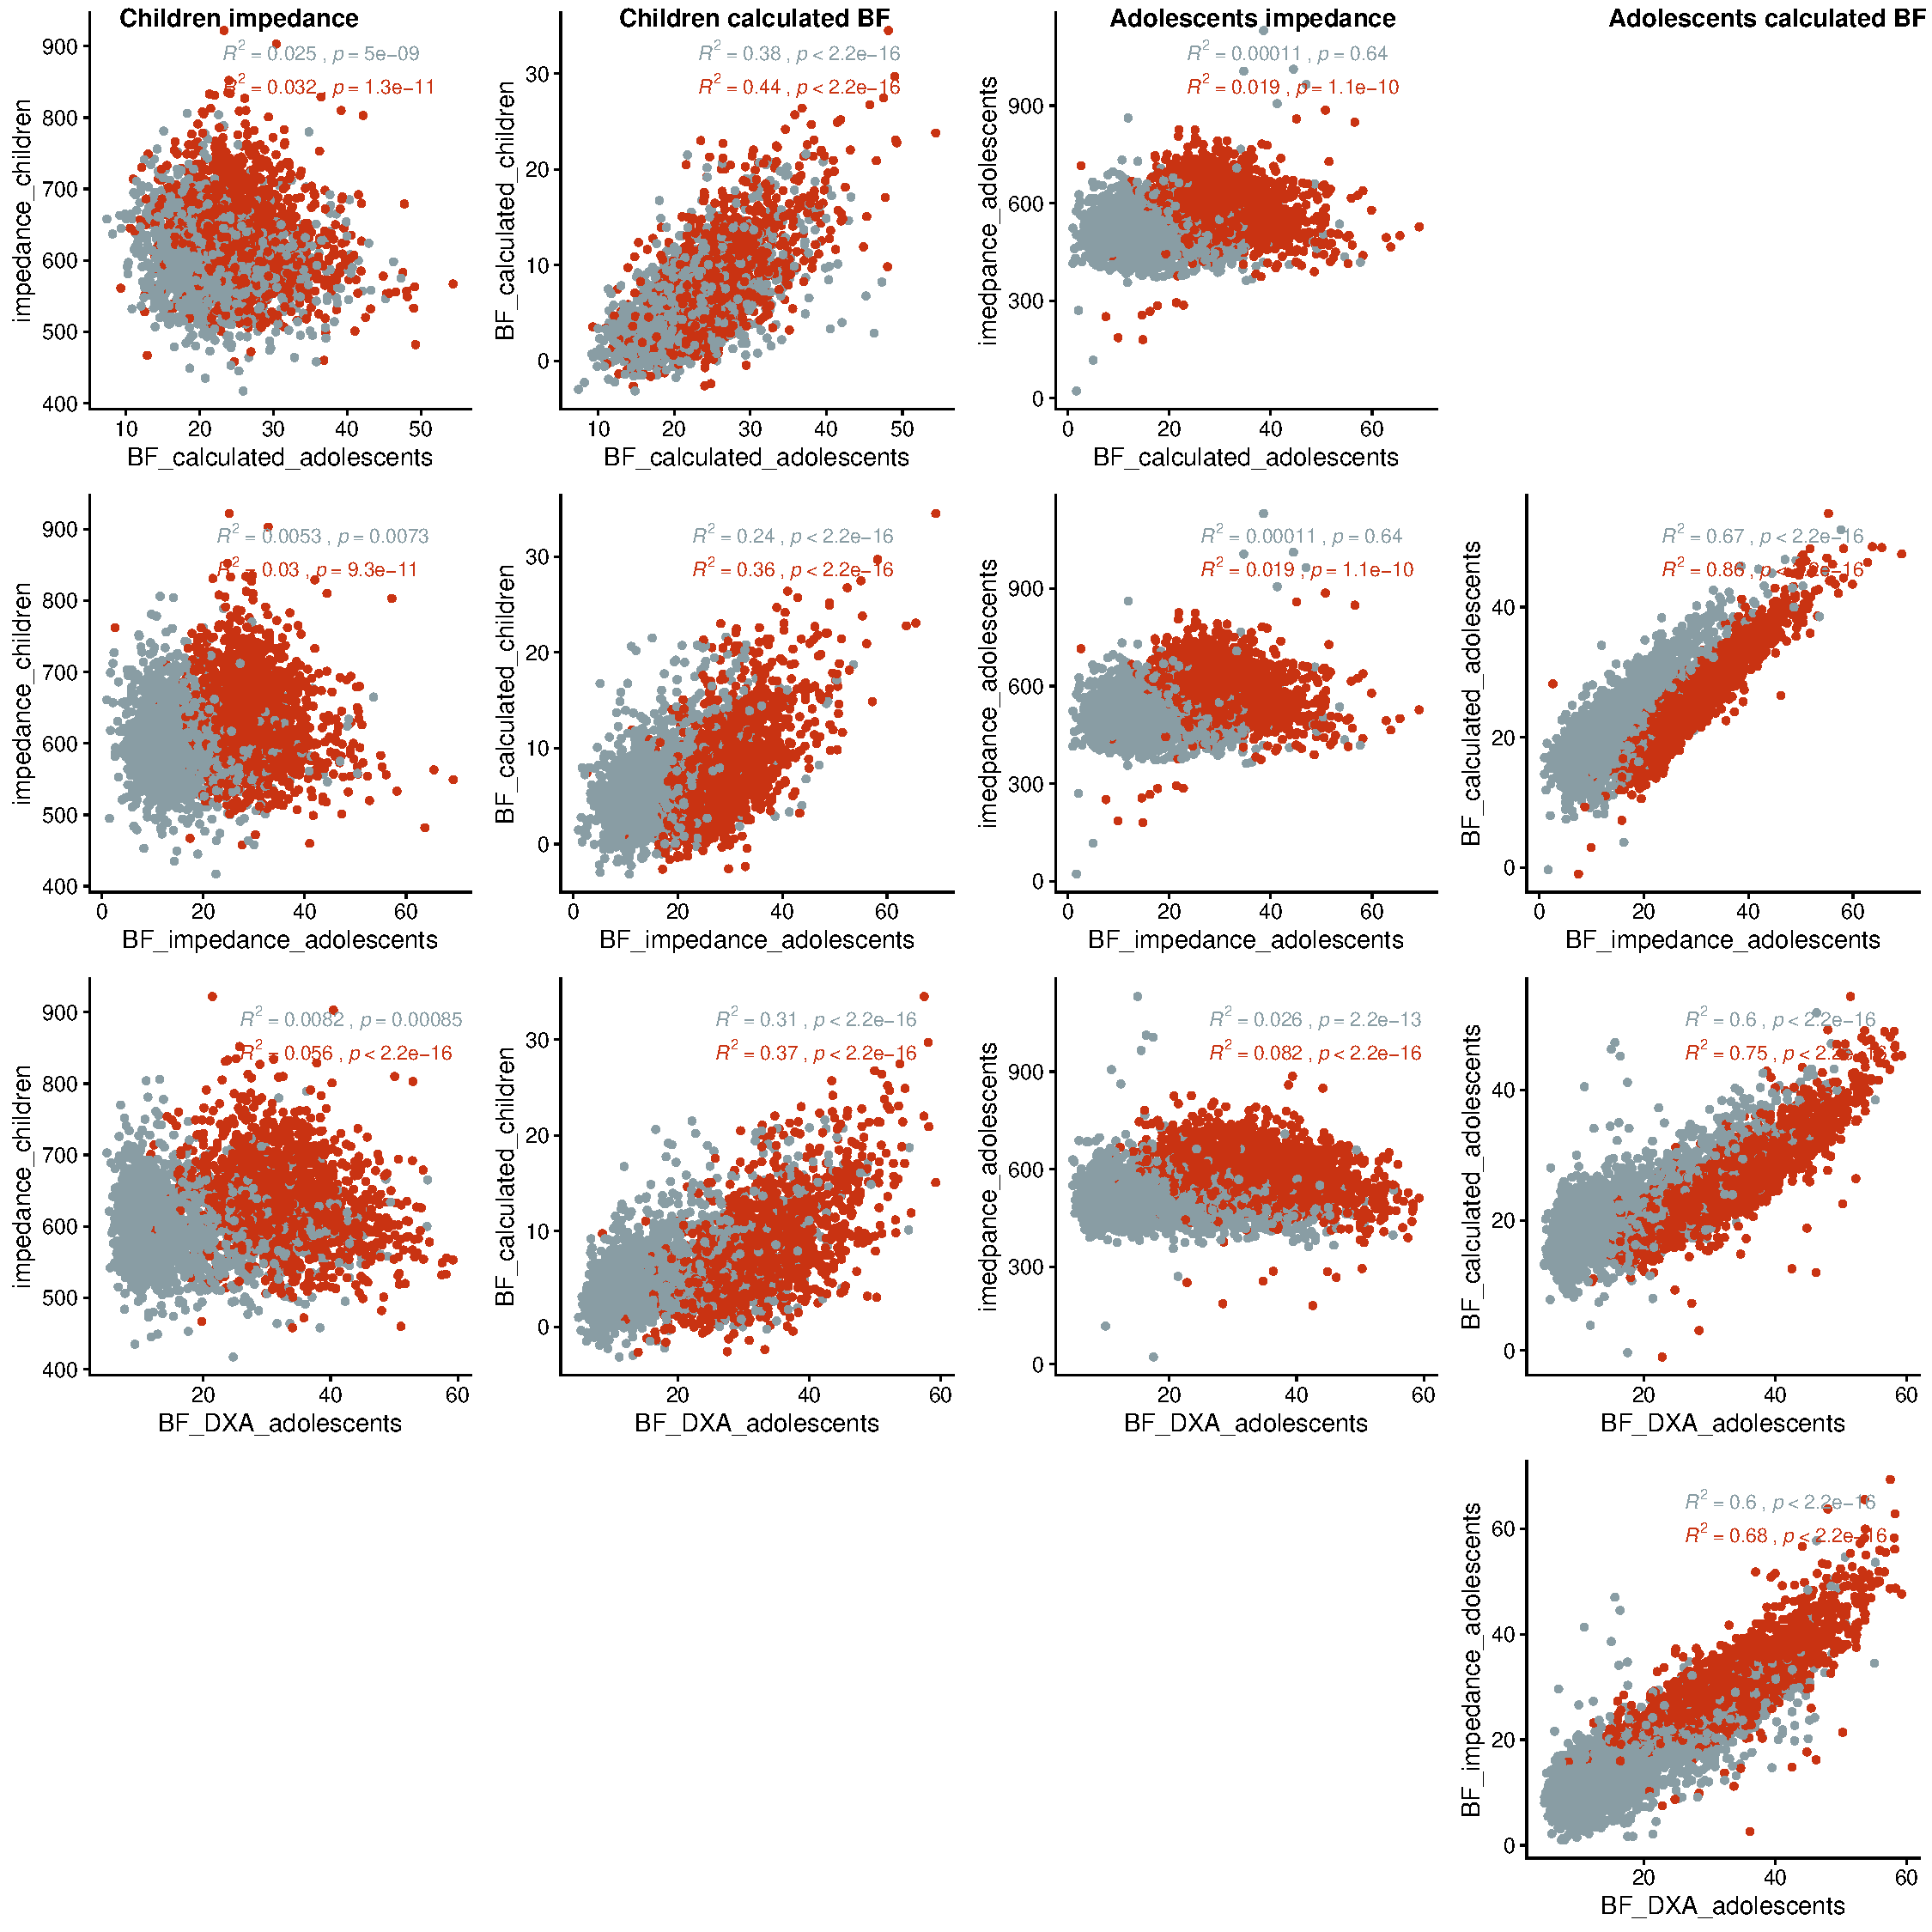
\includegraphics[width=1\linewidth]{data/chapter4/figures/bf_validation_correlation_bf} \caption{Correlation between differnet BF measures in children and adolescents}\label{fig:chapter4-figure-BF-validation-correlation-2}
\end{figure}
\noindent 
\bsmall
\emph{Figure \ref{fig:chapter4-figure-BF-validation-correlation-2} shows correlations for BF calculated using equation \eqref{eq:BF} in children and adolescents. Column 1 shows correlations between child impedance values and adolescent BF estimates. Column 2 shows correlations for child calculated BF and adolescent BF estimates. Column 3 shows correlations for adolescent calculated BF and adolescent BF estimates. Data is presented for complete cases across: QC'd metabolomics, BMI, WHR (children only), impedance, height, weight, age, sex, and BF derived by impedance and DXA in adolescents. Data for men is shown in grey and women in red.}
\esmall
\begin{figure}
\includegraphics[width=1\linewidth]{data/chapter4/figures/bf_validation_correlation} \caption{Correlation between BF and BMI, height, and weight in children and adolescents}\label{fig:chapter4-figure-BF-validation-correlation}
\end{figure}
\noindent 
\bsmall
\emph{Figure \ref{fig:chapter4-figure-BF-validation-correlation} shows correlations for impedance and BF for children (columns 1 and 2) and adolescents (columns 3-6) with BMI (top row), weight (middle row), and height (bottom row). BF\_calculates is BF derived using the raw impedance value measured in ohms and equation \eqref{eq:BF}. Data is presented for complete cases across: QC'd metabolomics, BMI, WHR (children only), impedance, height, weight, age, sex, and BF derived by impedance and DXA in adolescents. Data for men is shown in grey and women in red.}
\esmall

\hypertarget{statistical-analysis-1}{%
\subsection{Statistical analysis}\label{statistical-analysis-1}}

\hypertarget{directional-consistency-across-models-within-exposures-and-age-groups}{%
\subsubsection{Directional consistency: across models within exposures and age groups}\label{directional-consistency-across-models-within-exposures-and-age-groups}}

Across models within each exposure and age group a majority of tests resulted in directionally consistent effect estimates (Figure \ref{fig:chapter4-figure-directional-consistency}). Of these directionally consistent effects, the majority of effect estimates were positive. The strength of the effect estimates were broadly consistent across models; confidence intervals overlapped across the majority of metabolites for all models within each group and exposure (Supplementary \ref{chapter4-appendix-figures-forestplots}). Of the 220 metabolites measured in all age groups, directional consistency was supported by strong evidence of correlation across models within exposures and age groups (Supplement \ref{chapter4-appendix-correlations}).
\begin{figure}
\includegraphics[width=1\linewidth]{thesis_files/figure-latex/chapter4-figure-directional-consistency-1} \caption{Directional consistency across linear models}\label{fig:chapter4-figure-directional-consistency}
\end{figure}
\noindent 
\bsmall
\emph{Figure \ref{fig:chapter4-figure-directional-consistency} shows the directional consistency of all models for each group and exposure A positive effect reflects both model betas being in the positive direction; a negative effect reflects both model betas being in a negative direction; opposite effect reflects different directions for the model betas. BMI = body mass index; WHR = waist hip ratio; FFM = fat free mass; BF = body fat percentage.}
\esmall

\hypertarget{multiple-testing-threshold}{%
\subsubsection{Multiple testing threshold}\label{multiple-testing-threshold}}

Across all models and exposures, between 32.61 percent and 86.4 percent (median = 61.3 percent) of metabolites reached a multiple testing threshold (children multiple testing threshold = 42, adolescents = 42, young adults = 40, adults = 44; Table \ref{tab:chapter4-table-significant-results}). Of those with a consistent direction of effect across the three exposures a total of 109, 146, 164, and 180 metabolites reached a multiple testing threshold for children, adolescents, young adults, and adults respectively. This equates to 47, 63, 73, and 79 percent of metabolites.
\begin{longtable}[t]{lrrrllllrrl}
\caption{\label{tab:chapter4-table-significant-results}Metabolites reaching a multiple testing threshold}\\
\toprule
\multicolumn{2}{c}{ } & \multicolumn{3}{c}{BMI} & \multicolumn{3}{c}{WHR} & \multicolumn{3}{c}{BF} \\
\cmidrule(l{3pt}r{3pt}){3-5} \cmidrule(l{3pt}r{3pt}){6-8} \cmidrule(l{3pt}r{3pt}){9-11}
 & N & 1 & 2 & 3 & 1 & 2 & 3 & 1 & 2 & 3\\
\midrule
Children & 230 & 141 & 137 & -- & 148 & 148 & -- & 141 & 132 & --\\
Adolescents & 230 & 138 & 156 & 83 & -- & -- & -- & 150 & 159 & 75\\
Young adults & 224 & 173 & 172 & 139 & 173 & 172 & 139 & 183 & 180 & 135\\
Adults & 228 & 193 & 191 & 183 & 193 & 191 & 183 & 197 & 191 & 186\\
\bottomrule
\end{longtable}
\noindent 
\bsmall
\emph{Table \ref{tab:chapter4-table-significant-results} shows the number of metabolites reaching a multiple testing threshold for each model within each age group. Multiple testing thresholds: children = 54, adolescents = 48, young adults = 46, adults = 53. N = total number of metabolites tested; BMI = body mass index; WHR = waist hip ratio; BF = body fat percentage (in children this is fat free mass); 1 = model 1 adjustment for age and sex; 2 = model 2 adjustment for model 1 plus maternal/own education, smoking status, alcohol frequency, diet (where available); 3 = model 3, adjustment for model 2 plus physical activity (where available).}
\esmall

\hypertarget{directional-consistency-across-exposures-within-age-groups-for-model-2}{%
\subsubsection{Directional consistency: across exposures within age groups for model 2}\label{directional-consistency-across-exposures-within-age-groups-for-model-2}}

Results here on are presented for model 2 only; results for models 1 and 3 are presented in the supplement. Across exposures within each age group, effects showed mostly consistent directions of effect, with the majority being positive (Figure \ref{fig:chapter4-figure-directional-consistency-2}). The most inconsistent directions across exposures were found for children, where 21 percent of metabolites showed inconsistent directions of effect. For adolescents, young adults, and adults 5, 9, and 5 percent of metabolites showed inconsistent effect directions across measures of adiposity respectively. Of the 220 metabolites measured across all age groups, directional consistency was supported by strong evidence of correlation across exposures within age groups; though still strong, weaker correlations were observed when looking within exposures across age groups (Supplement \ref{chapter4-appendix-correlations}).
\begin{figure}
\includegraphics[width=1\linewidth]{thesis_files/figure-latex/chapter4-figure-directional-consistency-2-1} \caption{Directional consistency across exposures within each age group}\label{fig:chapter4-figure-directional-consistency-2}
\end{figure}
\noindent 
\bsmall
\emph{Figure \ref{fig:chapter4-figure-directional-consistency-2} shows the directional consistency of all exposures for each age group. A positive effect reflects effect estimates for all exposures being in the positive direction; a negative effect reflects effect estimates being in the negative direction; opposite effect reflects different directions for the effect estimates across the exposures.}
\esmall
\noindent 

\hypertarget{global-metabolic-profile}{%
\subsubsection{Global metabolic profile}\label{global-metabolic-profile}}

Globally, the pattern of association was very similar for all measures of adiposity for children (Figure \ref{fig:chapter4-figure-circosplot-main-children}), adolescents (Figure \ref{fig:chapter4-figure-circosplot-main-adolescents}), young adults (Figure \ref{fig:chapter4-figure-circosplot-main-young-adults}), and adults (Figure \ref{fig:chapter4-figure-circosplot-main-adults}). Across all age groups the largest effects were found for the \emph{Fatty Acids} subclass; total fatty acids showed the largest effect for all age groups. Metabolites in subclasses \emph{small VLDL}, \emph{medium VLDL}, \emph{large VLDL}, and \emph{very large VLDL} were the only ones to reach the specified significance thresholds across all exposures and age groups. Effect estimates for derived measures were much higher for all exposures and age groups than with the subclasses presented here (Supplementary \ref{chapter4-appendix-circosplot-supplement2}). There was also considerable variation within subclasses for derived measures. The largest effect across all age groups and exposures among derived measures was observed for \emph{Cholesterol esters in very large VLDL to total lipids in very large VLDL ratio} and \emph{Total cholesterol in very large VLDL to total lipids in very large VLDL ratio}. Across age groups, direction of effect was consistent for the majority of metabolites within exposures (Supplementary \ref{chapter4-appendix-figures-forestplots}). On the whole, effect sizes were lowest in children and increased with age. The largest effect in adults, \emph{Total fatty acids} (beta = 0.51), was over twice that observed in children (beta = 0.21).
\begin{figure}
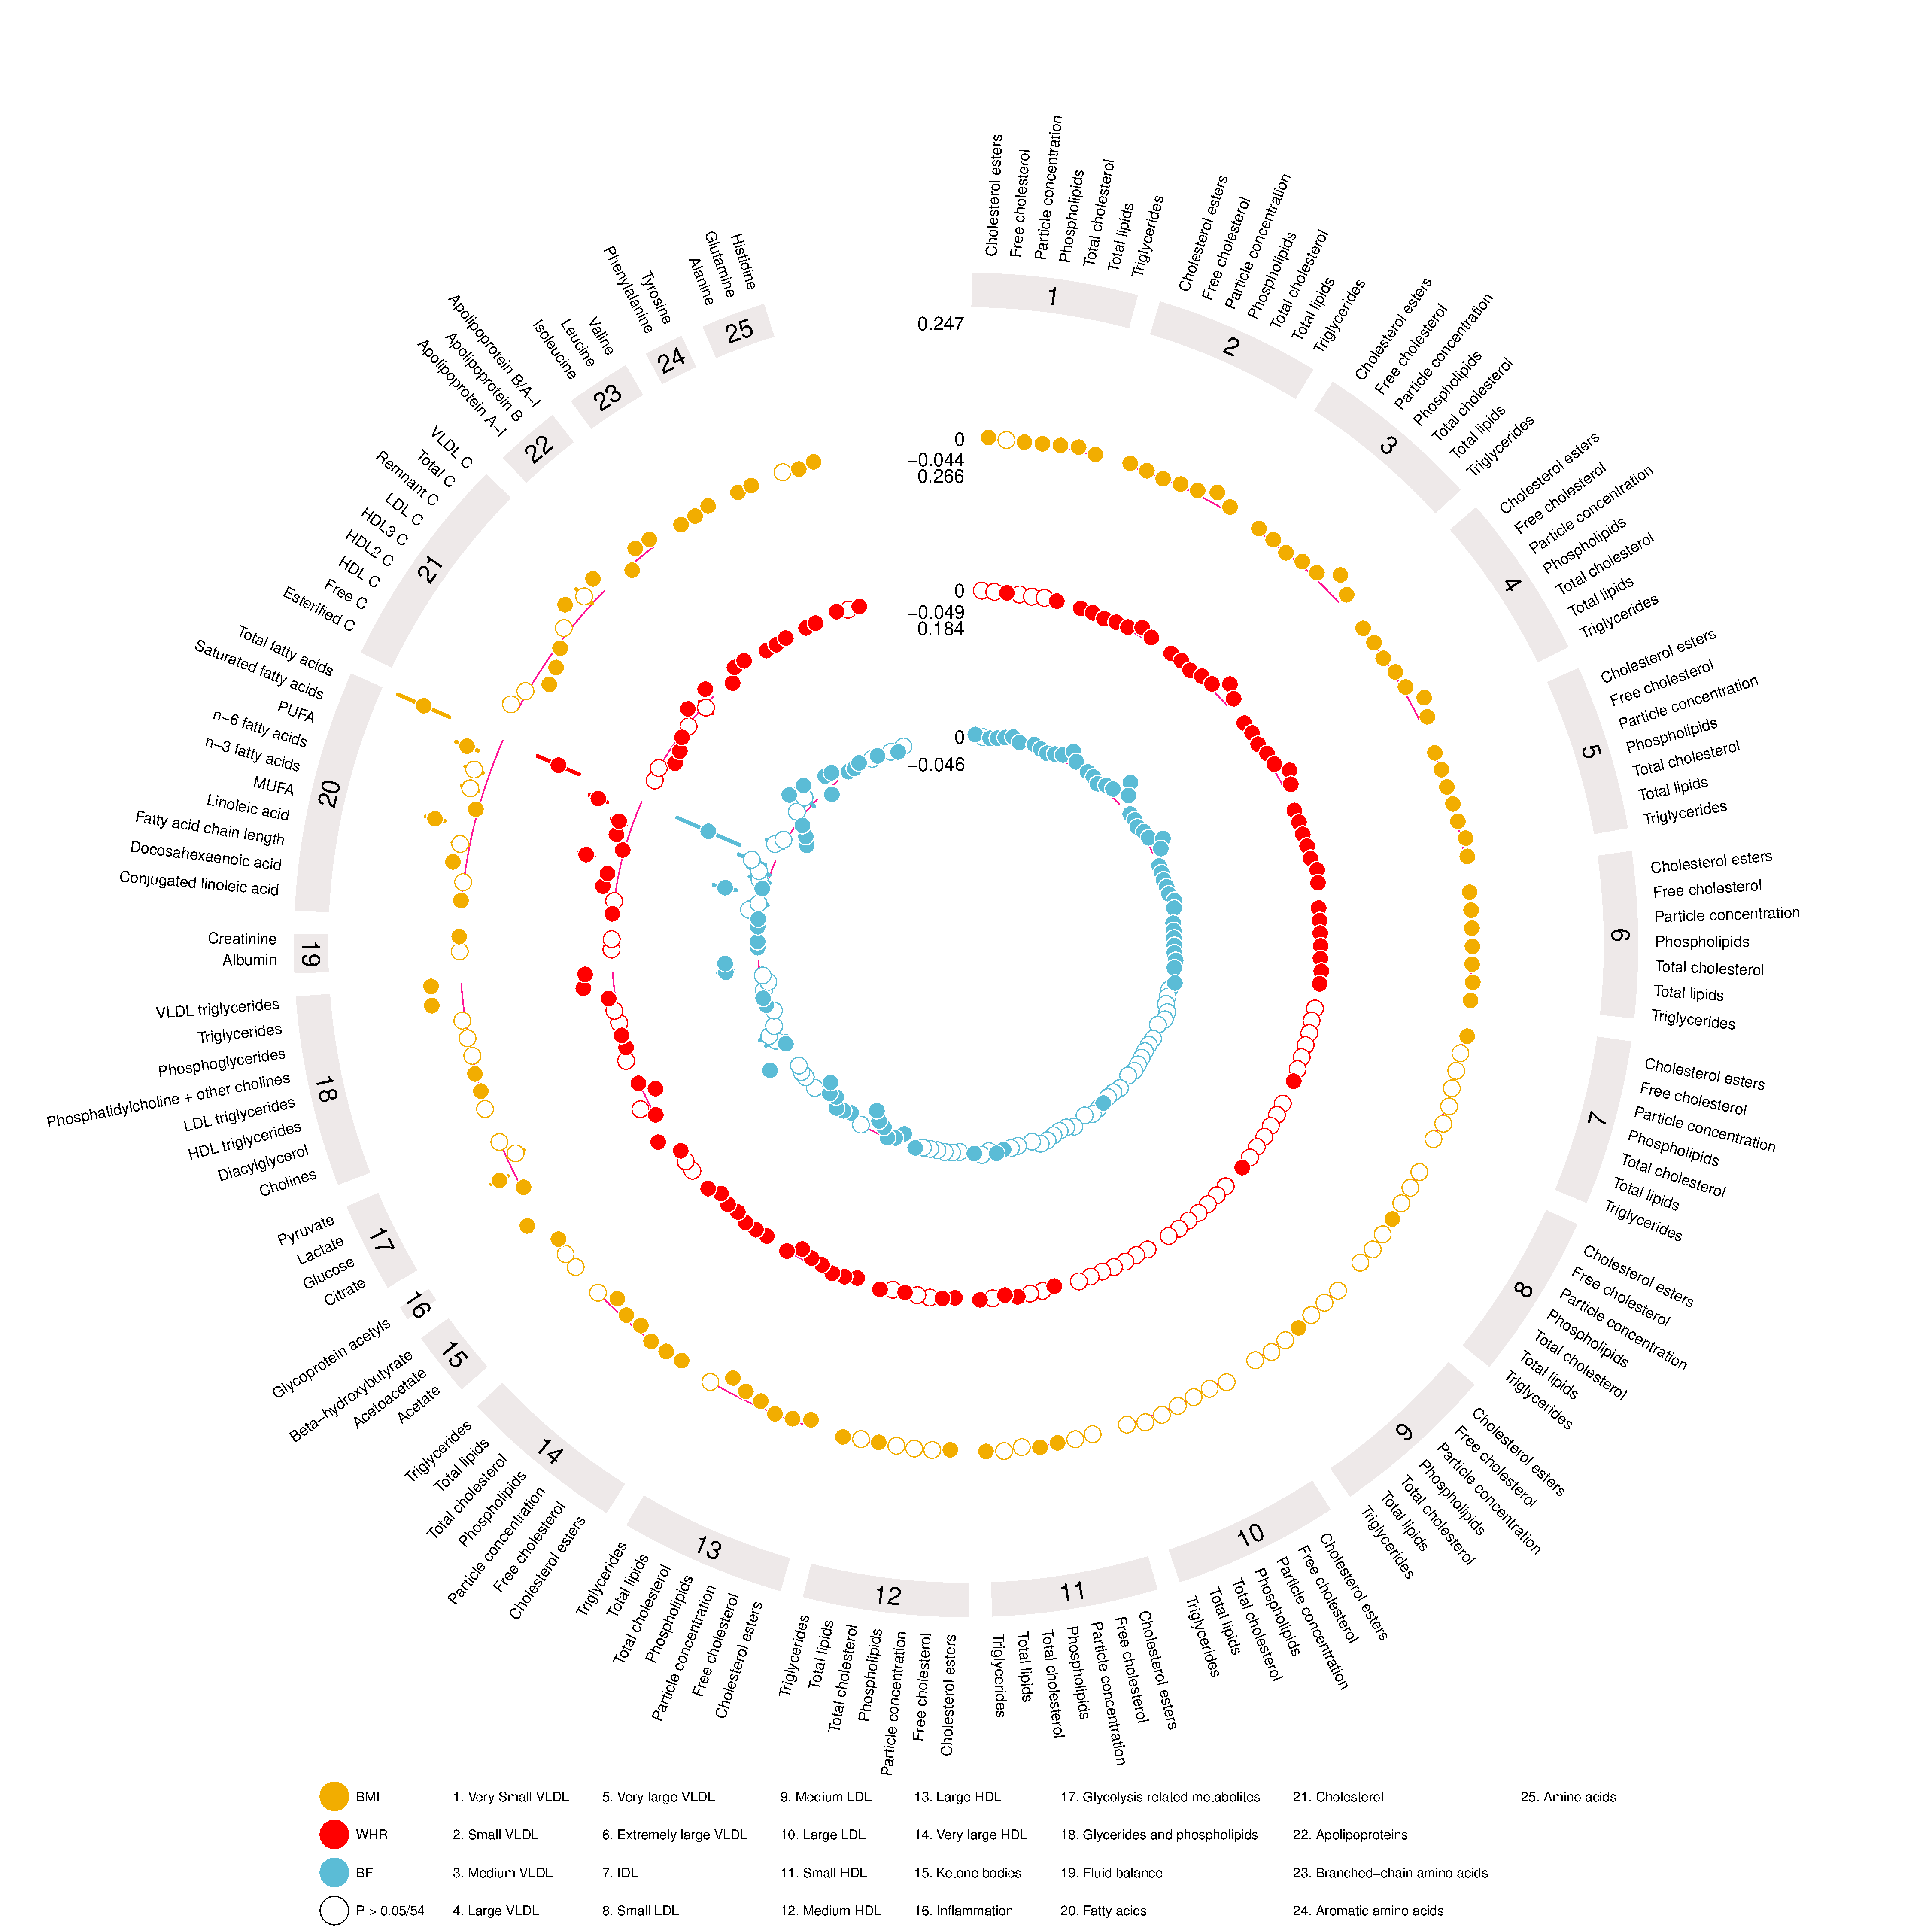
\includegraphics[width=1\linewidth]{data/chapter4/figures/circosplot_main_children} \caption{Circos plot of effect estimates from a linear regression of measures of increased adipsoity and metabolites in children}\label{fig:chapter4-figure-circosplot-main-children}
\end{figure}
\noindent 
\bsmall
\emph{Figure \ref{fig:chapter4-figure-circosplot-main-children} shows each track as one of the measures of adiposity; the outer track is BMI, the middle track is WHR, the inner track is BF. Solid points indicate a multiple testing threshold has been reached -- threshold set to the lowest of the age groups (54).}
\esmall
\begin{figure}
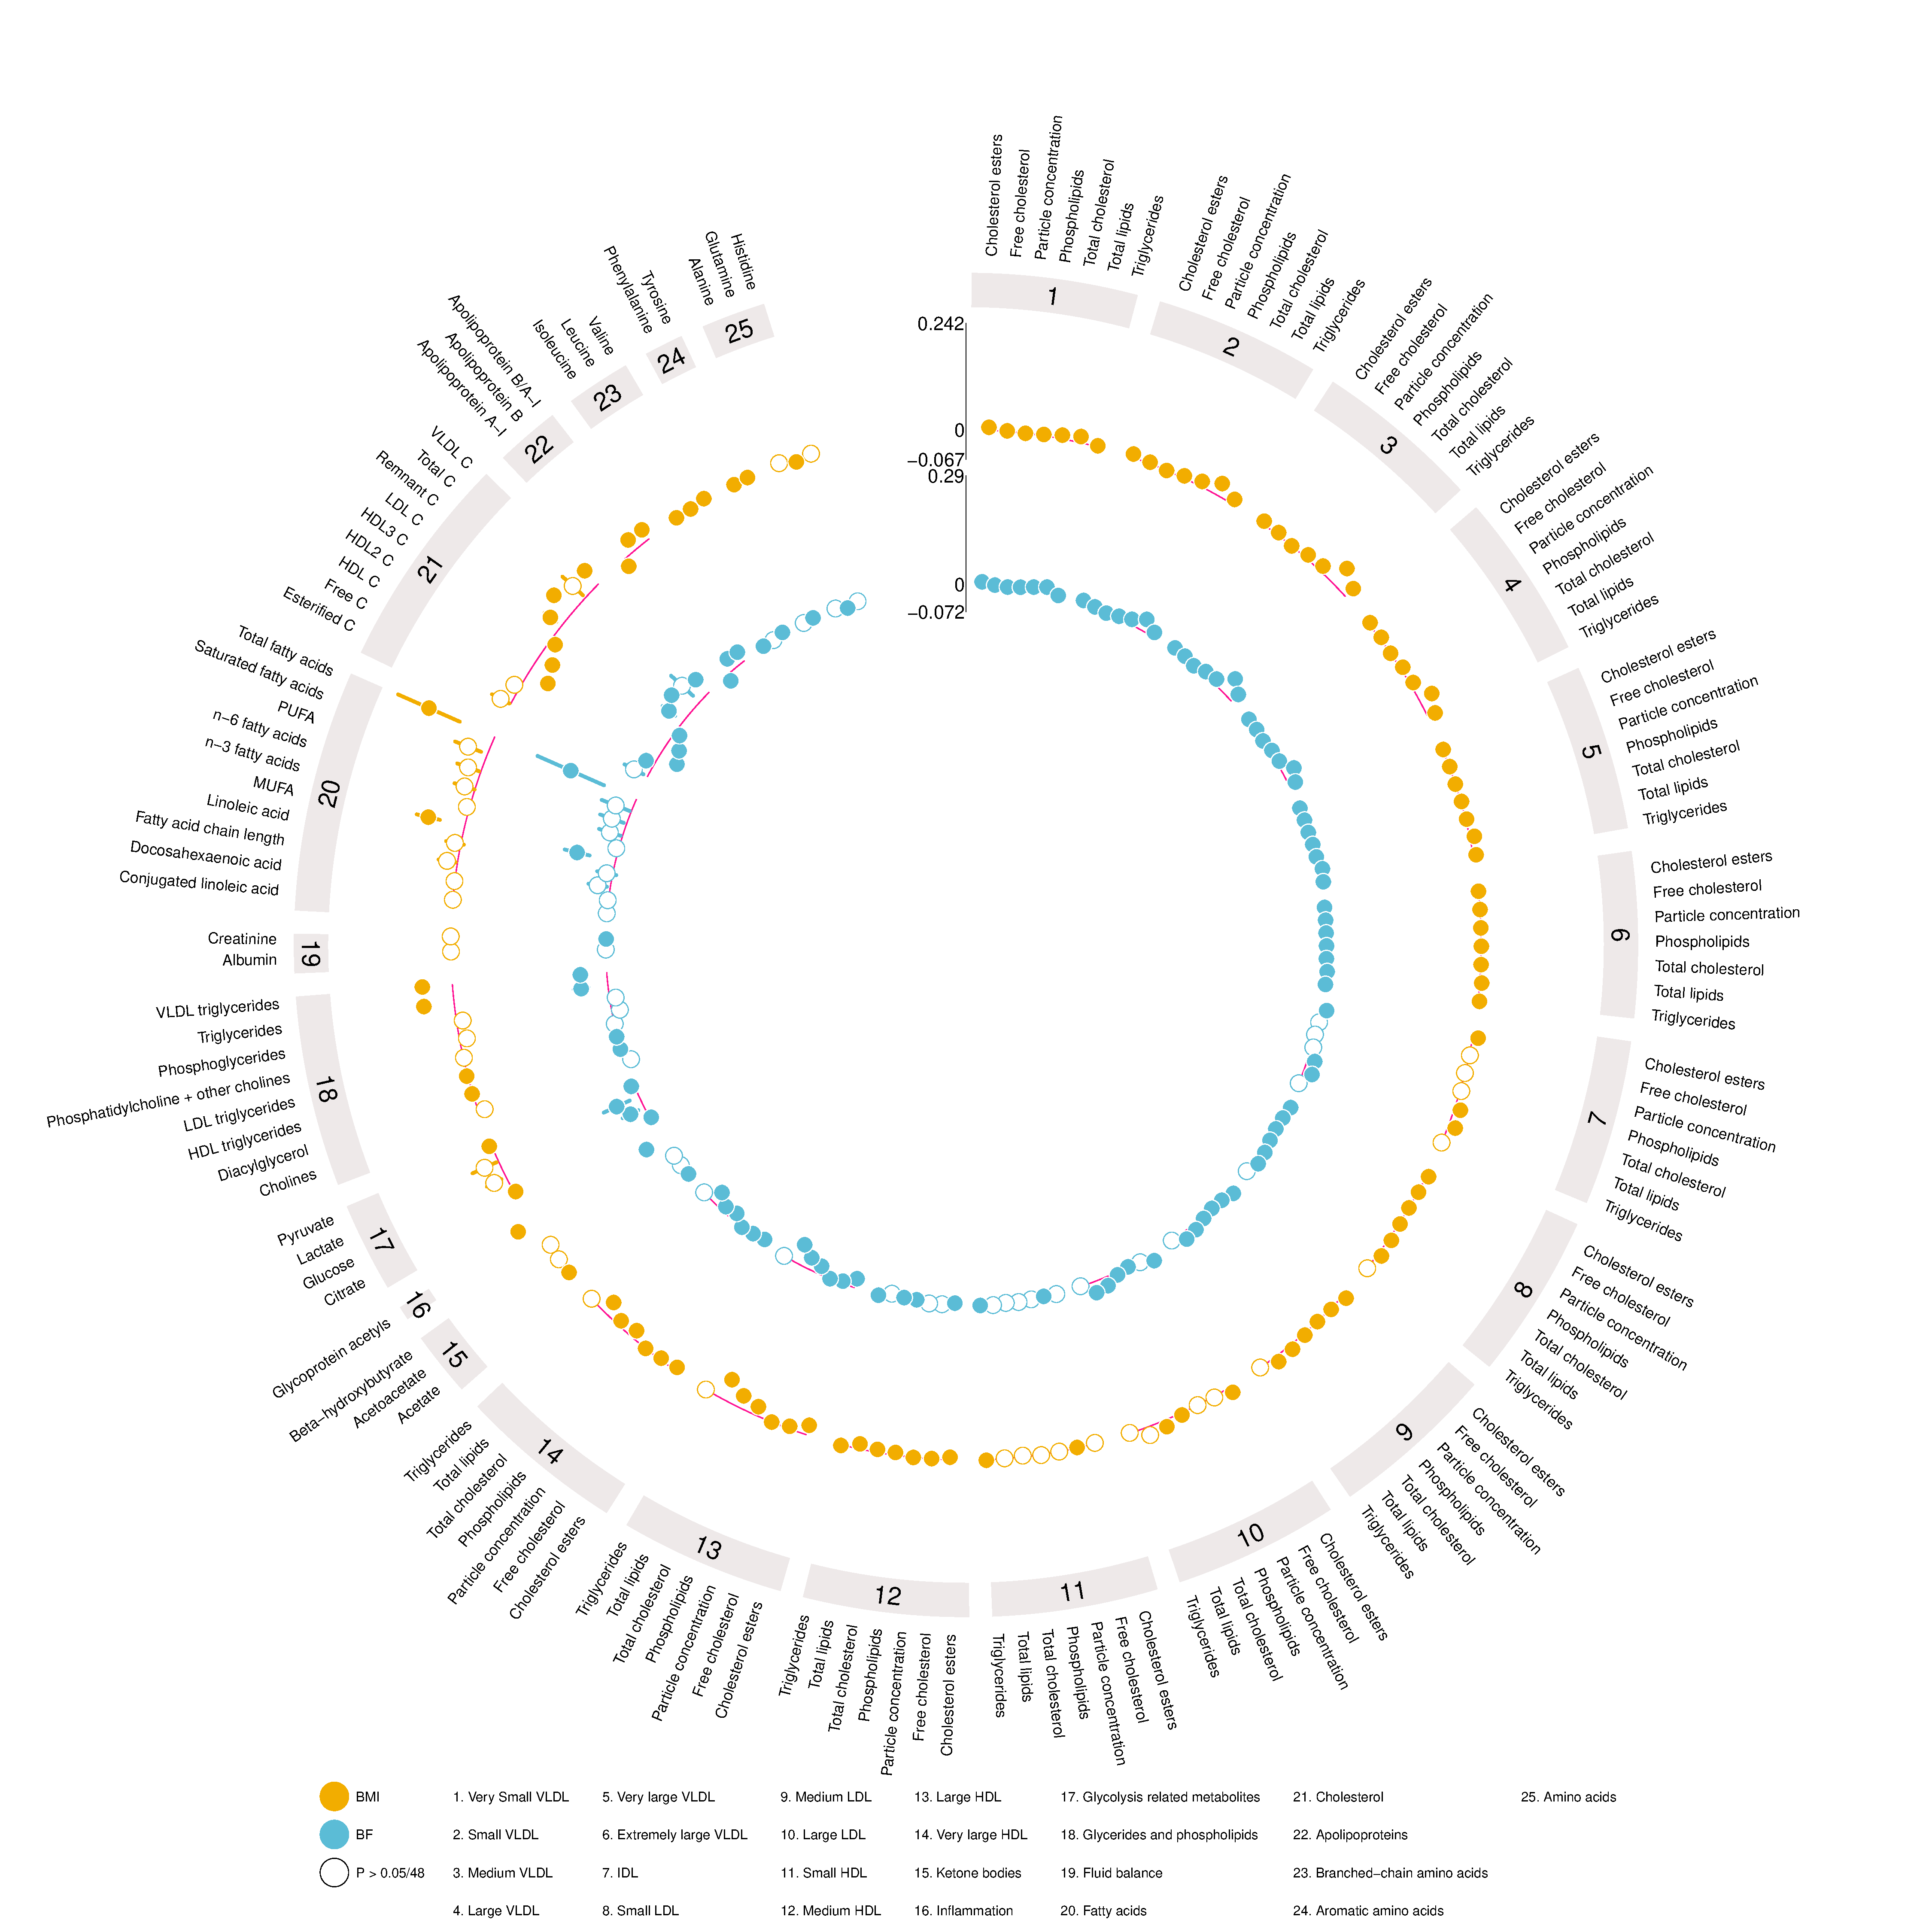
\includegraphics[width=1\linewidth]{data/chapter4/figures/circosplot_main_adolescents} \caption{Circos plot of effect estimates from a linear regression of measures of increased adipsoity and metabolites in adolescents}\label{fig:chapter4-figure-circosplot-main-adolescents}
\end{figure}
\noindent 
\bsmall
\emph{Figure \ref{fig:chapter4-figure-circosplot-main-adolescents} shows each track as one of the measures of adiposity; the outer track is BMI, the other track is BF - WHR was not available for adolescents. Solid points indicate a multiple testing threshold has been reached -- threshold set to the lowest of the age groups (48).}
\esmall
\begin{figure}
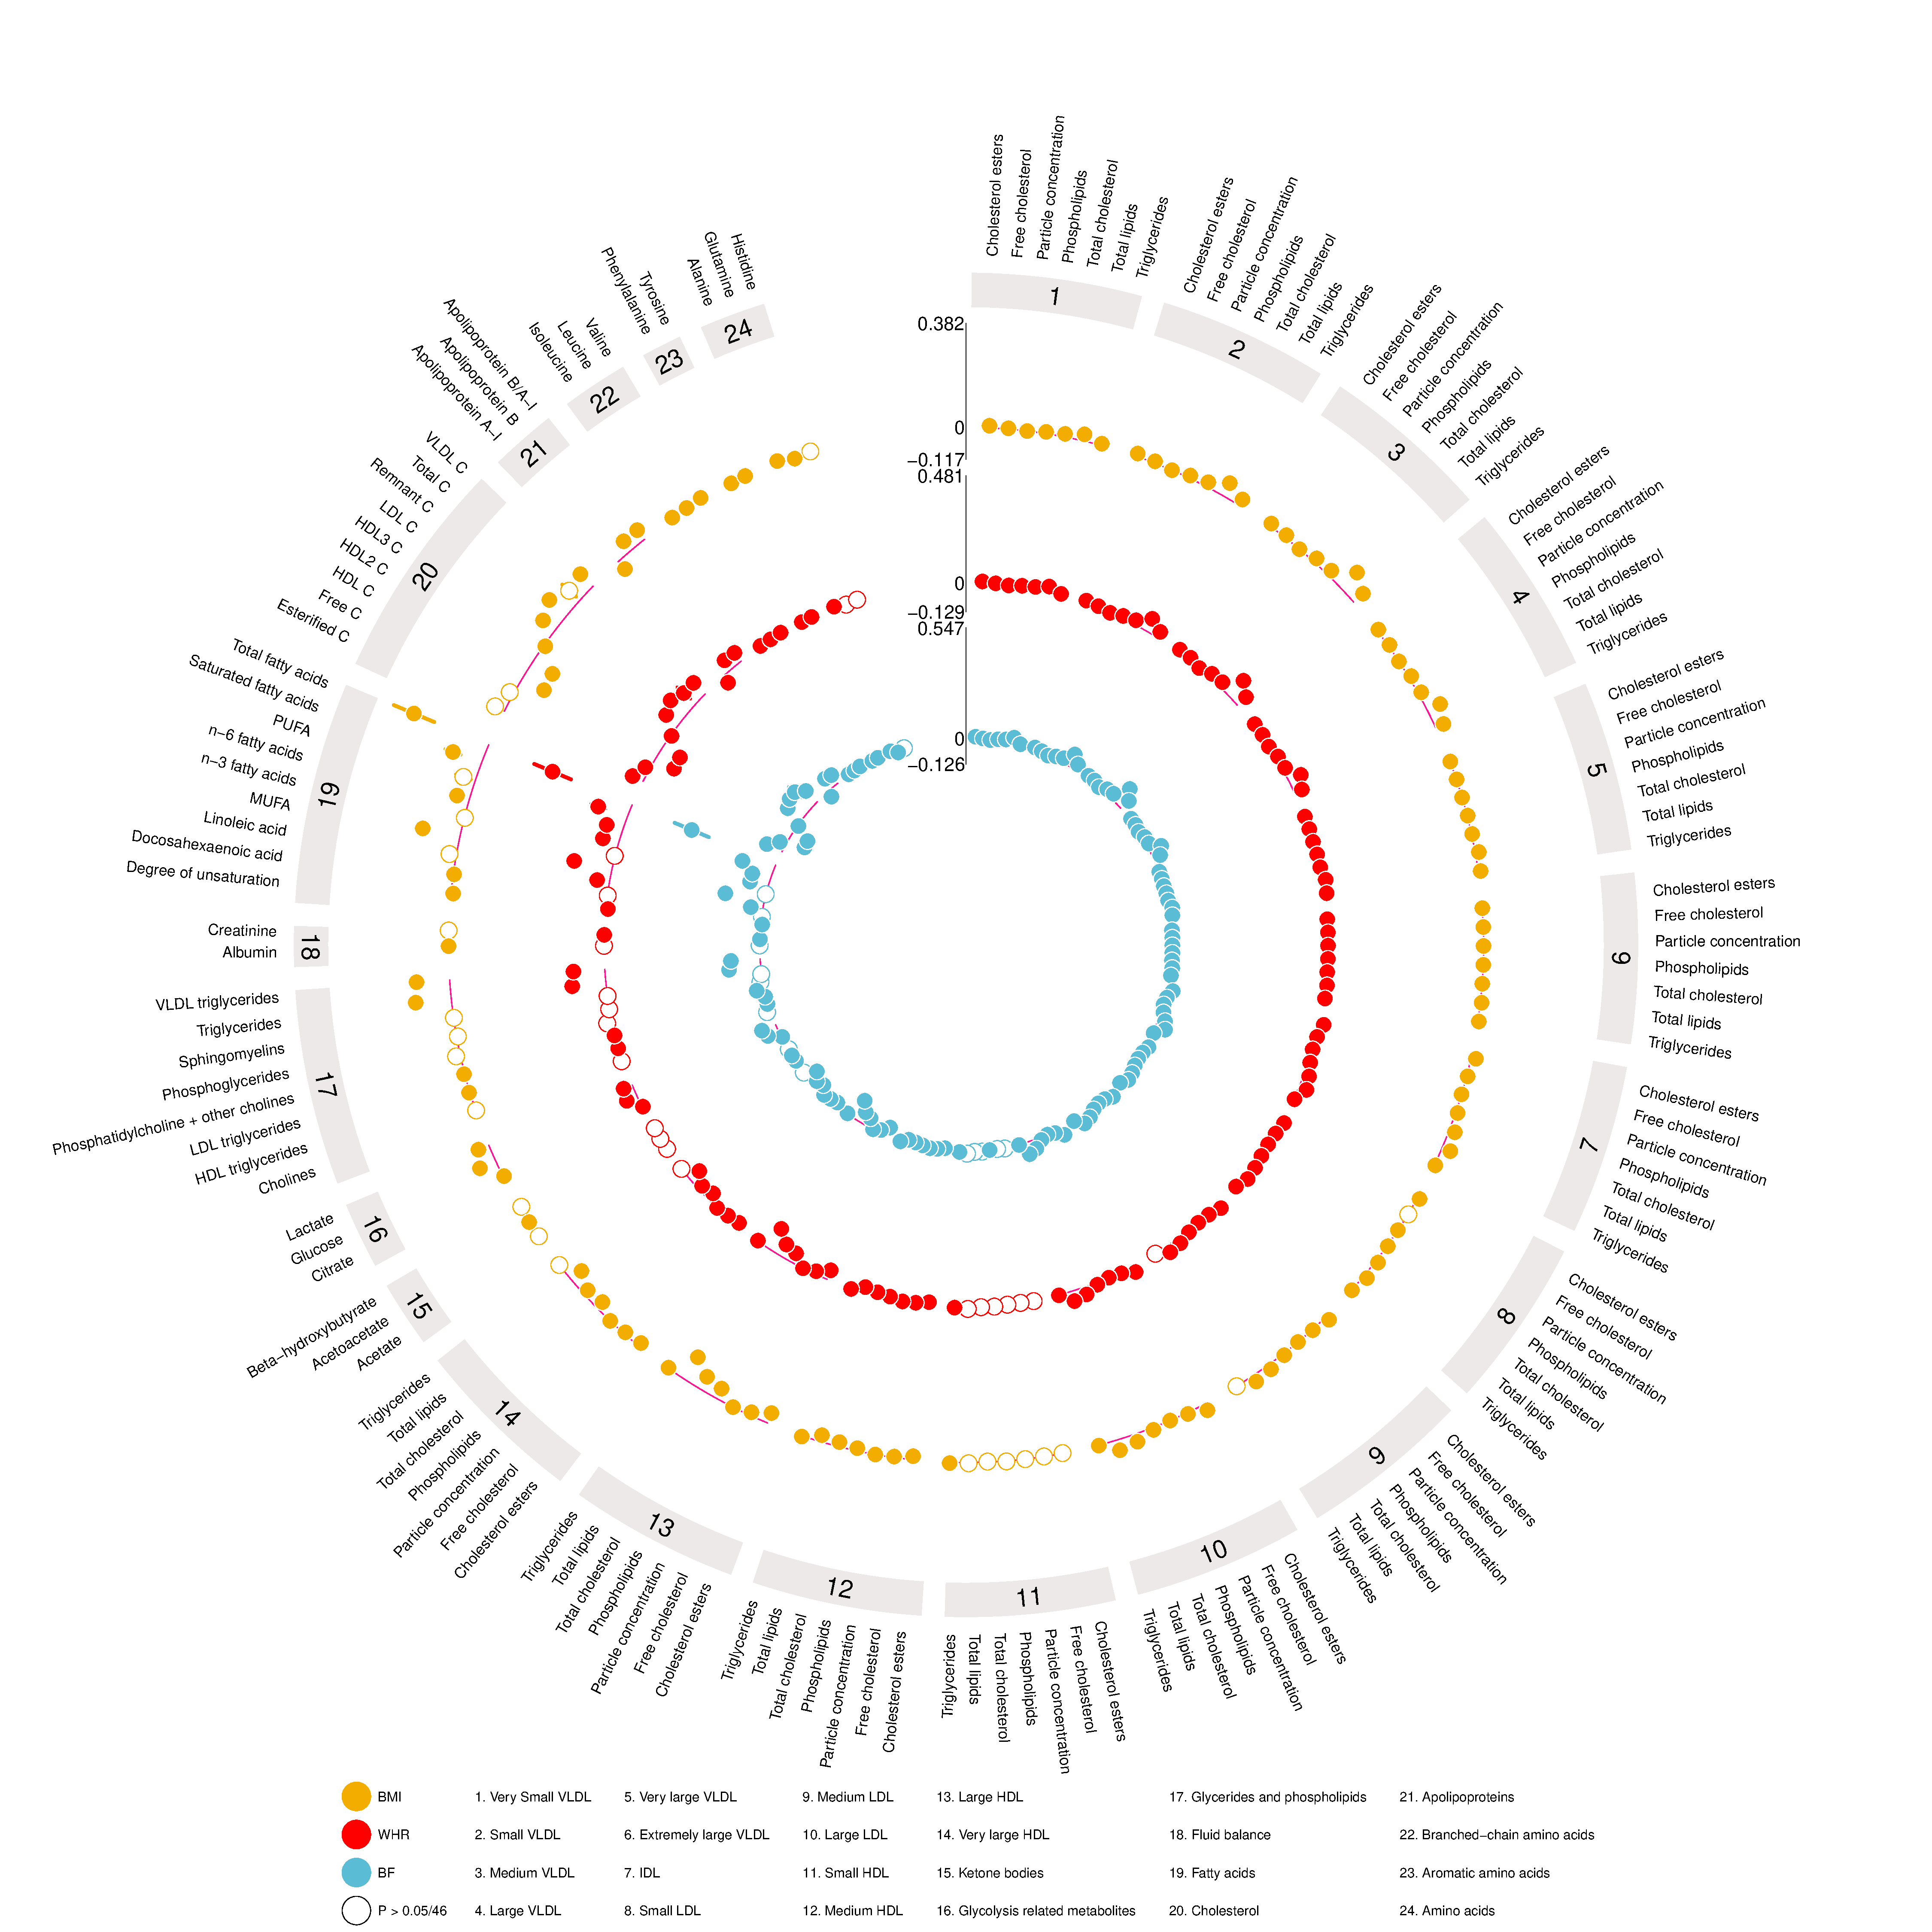
\includegraphics[width=1\linewidth]{data/chapter4/figures/circosplot_main_young_adults} \caption{Circos plot of effect estimates from a linear regression of measures of increased adipsoity and metabolites in young adults}\label{fig:chapter4-figure-circosplot-main-young-adults}
\end{figure}
\noindent 
\bsmall
\emph{Figure \ref{fig:chapter4-figure-circosplot-main-young-adults} shows each track as one of the measures of adiposity; the outer track is BMI, the middle track is WHR, the inner track is BF. Solid points indicate a multiple testing threshold has been reached -- threshold set to the lowest of the age groups (46).}
\esmall
\begin{figure}
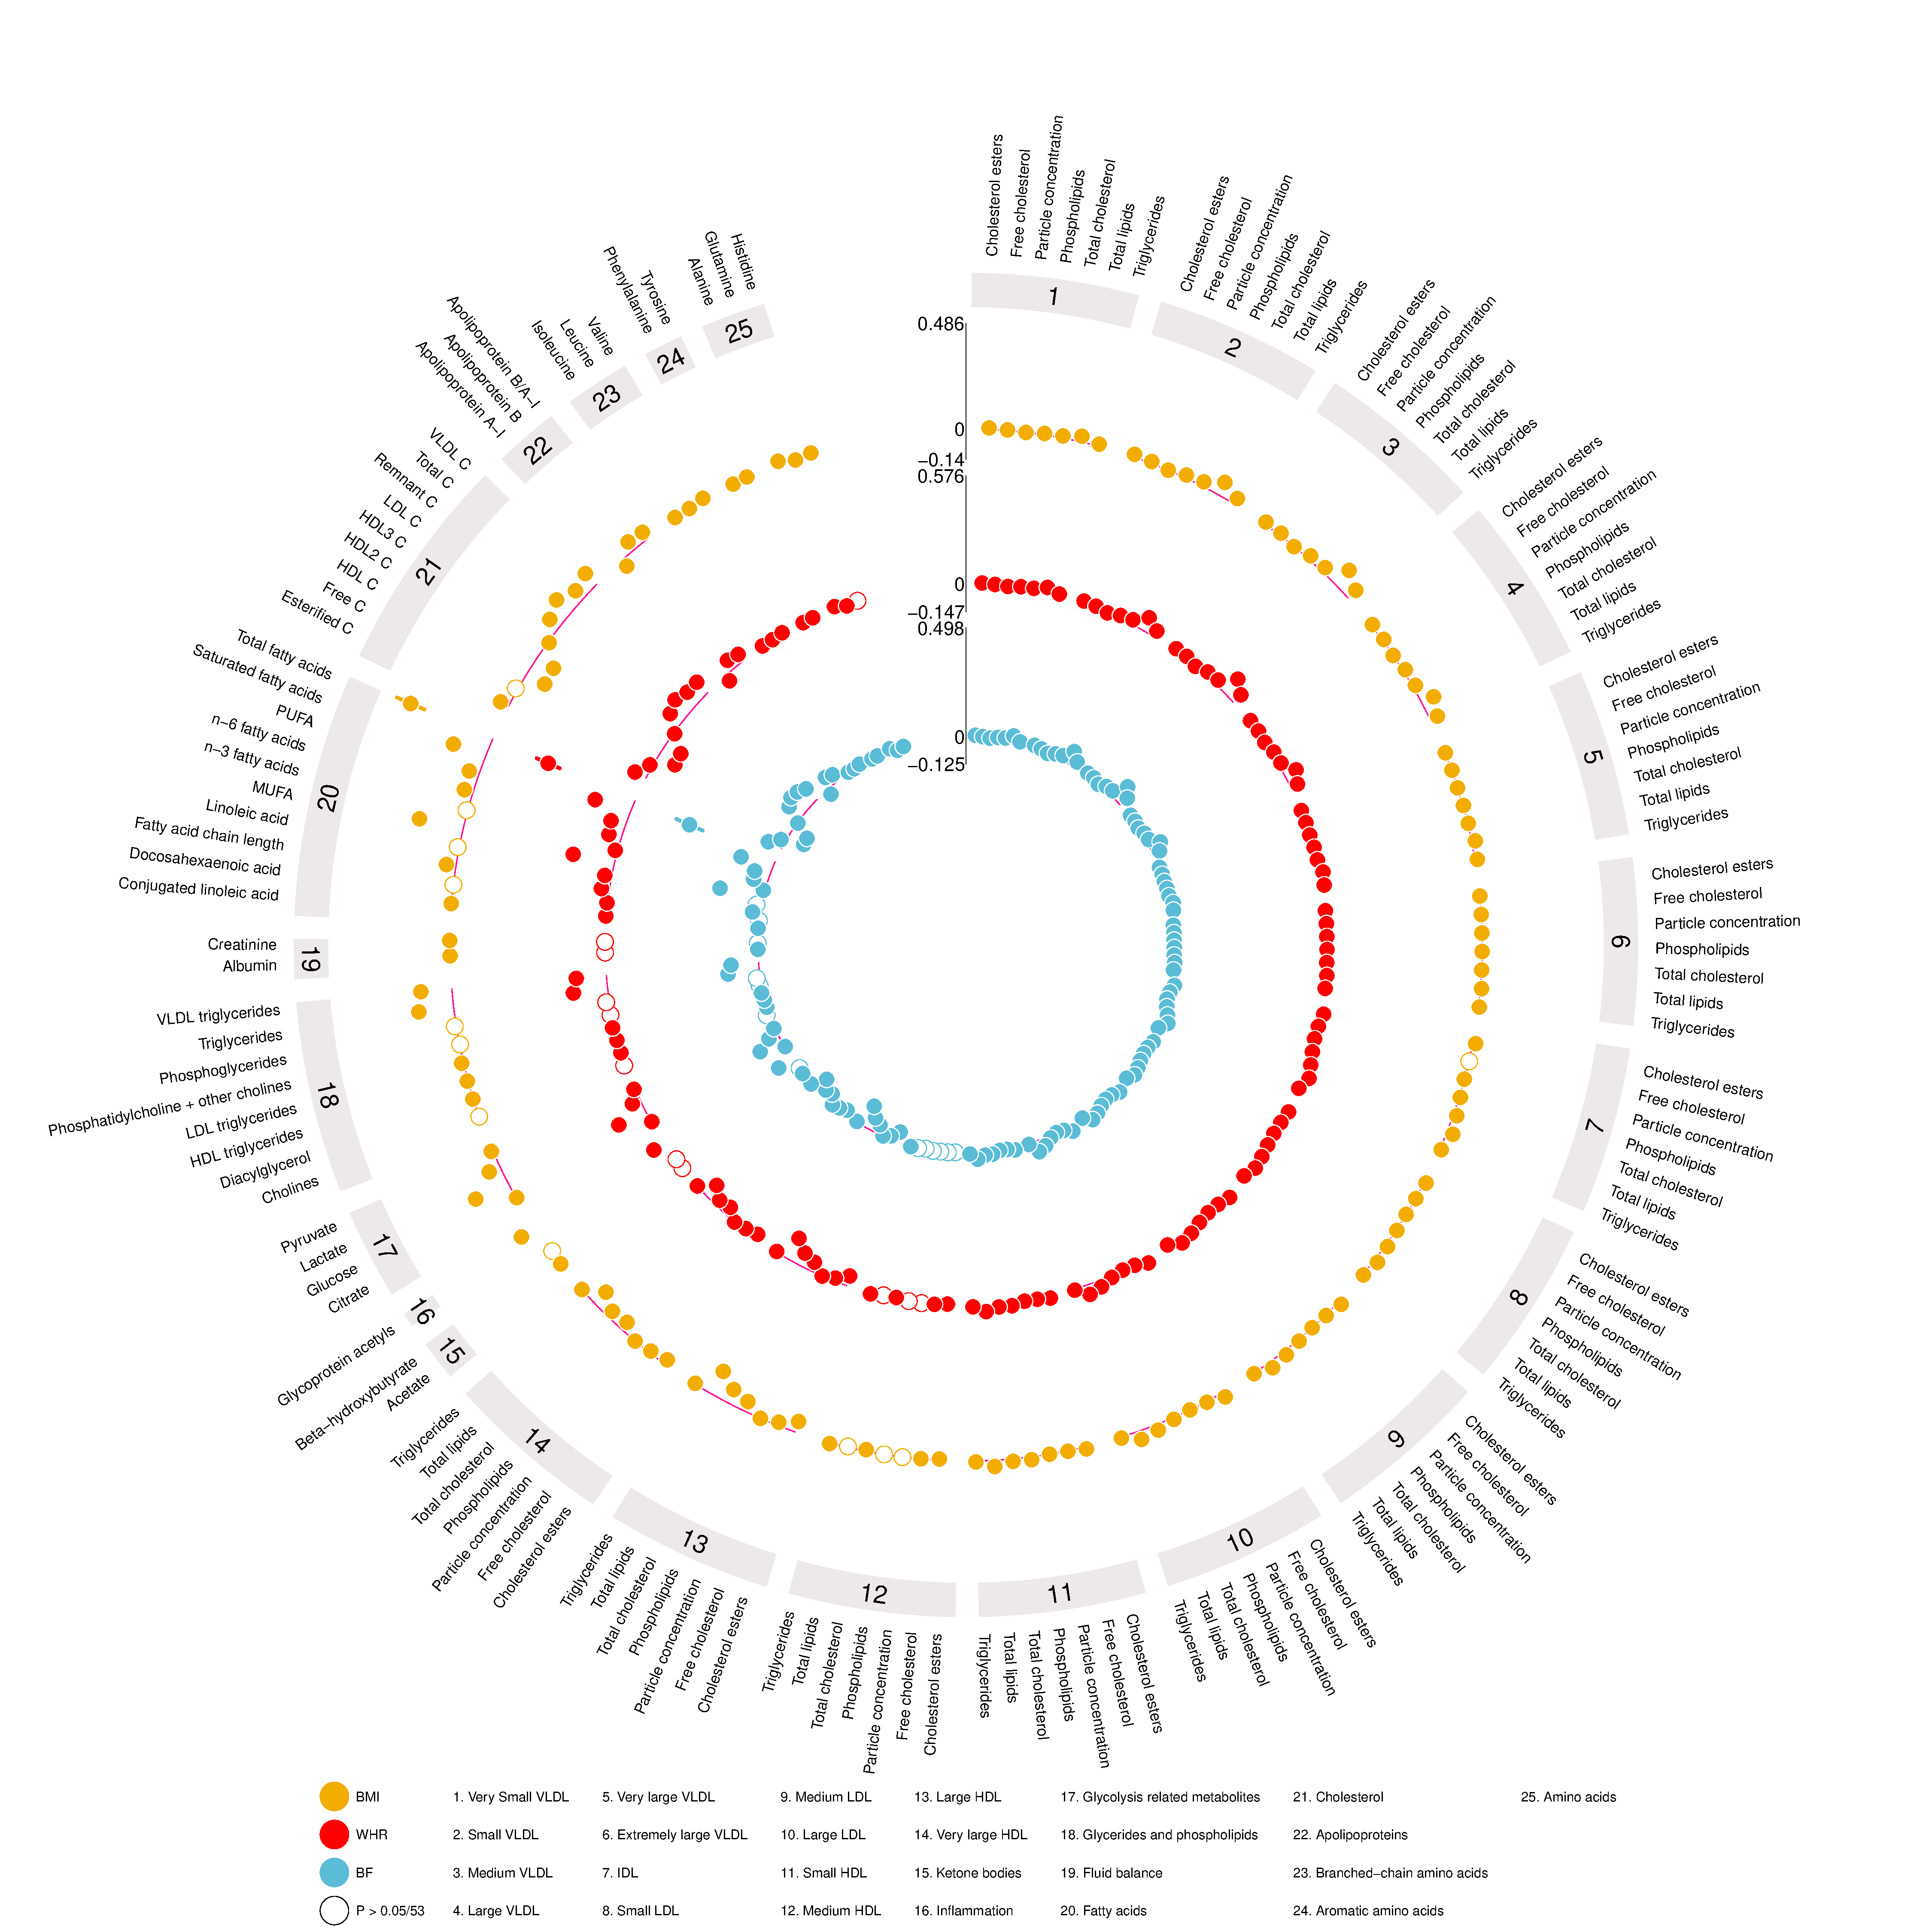
\includegraphics[width=1\linewidth]{data/chapter4/figures/circosplot_main_adults} \caption{Circos plot of effect estimates from a linear regression of measures of increased adipsoity and metabolites in adults}\label{fig:chapter4-figure-circosplot-main-adults}
\end{figure}
\noindent 
\bsmall
\emph{Figure \ref{fig:chapter4-figure-circosplot-main-adults} shows each track as one of the measures of adiposity; the outer track is BMI, the middle track is WHR, the inner track is BF. Solid points indicate a multiple testing threshold has been reached -- threshold set to the lowest of the age groups (53).}
\esmall

\hypertarget{subclass-results}{%
\subsubsection{Subclass results}\label{subclass-results}}

At the level of the subclass, associations were observed for all measures of adiposity across age groups and every subclass except \emph{Large LDL} in children, where weak evidence of association was observed across measures of adiposity. Across the derived measures, associations were observed across measures of adiposity for all subclasses except \emph{Extremely large VLDL ratios} in young adults and adults.

Across all age groups and exposures associations with every metabolite in a particular subclass was observed for \emph{Small VLDL}, \emph{Medium VLDL}, \emph{Large VLDL}, \emph{Very large VLDL}, and \emph{Extremely large VLDL} (Figure \ref{fig:chapter4-figure-forestplot-subclass-LDL}). As age increased, the number of associations within subclasses tended to increase across all measures of adiposity. For example, across \emph{Small LDL}, \emph{Medium LDL}, and \emph{Large LDL} few associations were observed across measures of adiposity in children, however in adolescents and young adults a majority of metabolites showed evidence of association while in adults all metabolites showed evidence of association.
\begin{figure}
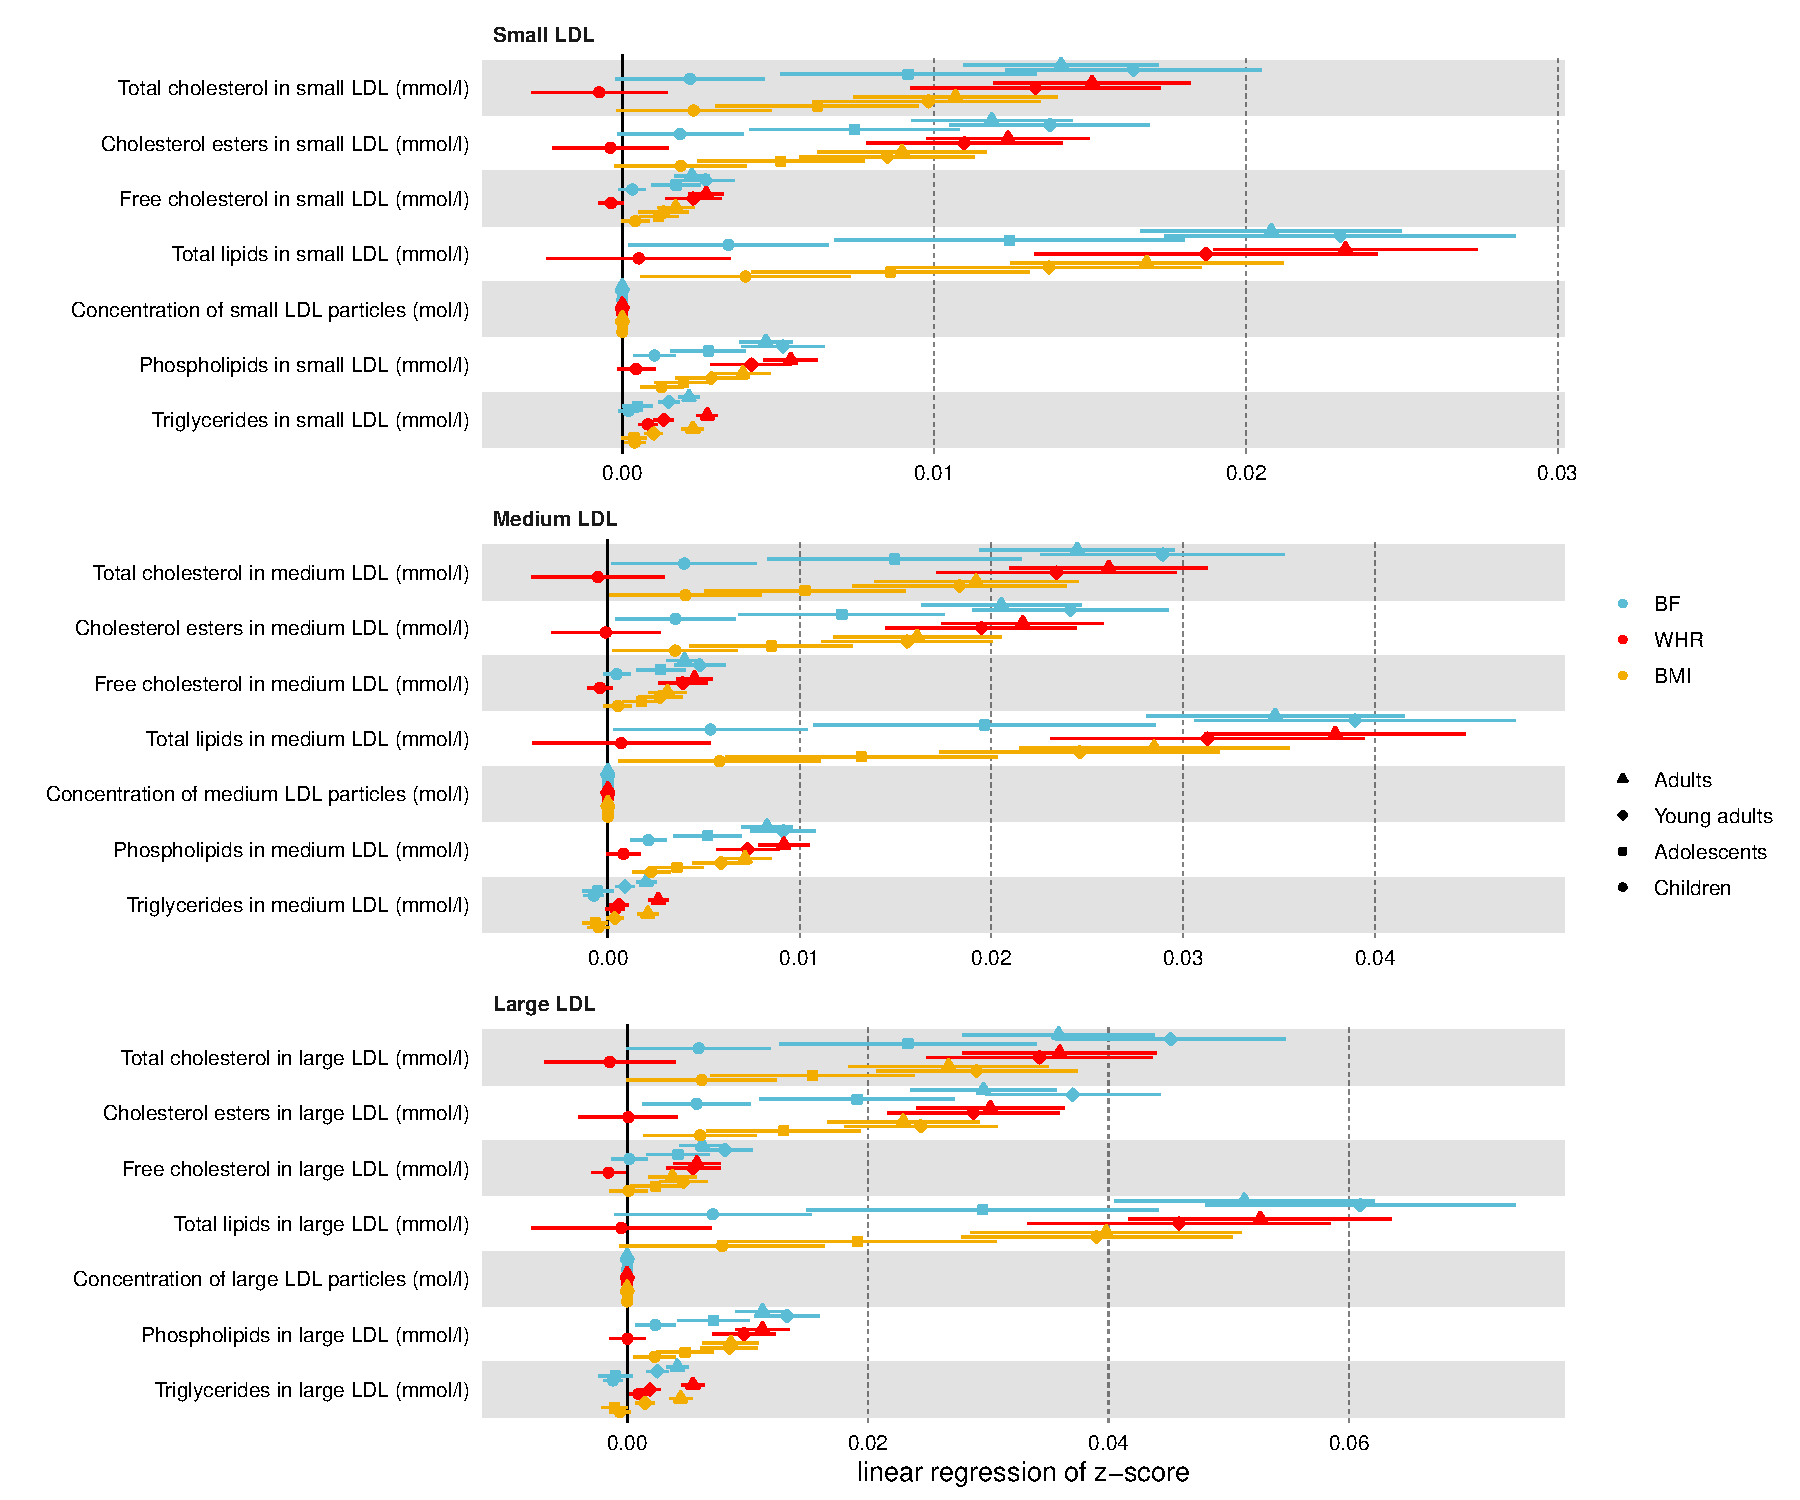
\includegraphics[width=1\linewidth]{data/chapter4/figures/forestplot_subclass_LDL} \caption{Forestplot of effect estimates across exposures and ages for LDL subclasses}\label{fig:chapter4-figure-forestplot-subclass-LDL}
\end{figure}
\noindent 
\bsmall
\emph{Figure \ref{fig:chapter4-figure-forestplot-subclass-LDL} gives the effect estimate and 95\% confidence interval for model 2 across all exposures and age groups.}
\esmall

\hypertarget{individual-results}{%
\subsubsection{Individual results}\label{individual-results}}

Excluding derived measures, \emph{Fatty acids ratios}, and \emph{Lipoprotein particle size} subclasses, which showed much larger and varied effects compared to other subclasses, effects ranged from -0.12 to 1 with a median of 0.003. The largest positive effects (\(> 0.1\)) were seen for Total fatty acids and mono-unsaturated fatty acids; the largest negative effects (\(< -0.1\)) were for Total lipids in large HDL and Total cholesterol in HDL (Table \ref{tab:chapter4-table-largest-effects}).

\blandscape
\begin{longtabu} to \linewidth {>{\raggedright\arraybackslash}p{15em}>{\raggedright\arraybackslash}p{5em}>{\raggedright\arraybackslash}p{5em}>{\raggedright}X>{\raggedleft}X>{\raggedleft}X>{\raggedleft}X}
\caption{\label{tab:chapter4-table-largest-effects}Largest effects (<= -0.1 and => 0.1) found across exposures and age groups}\\
\toprule
Metabolite & Subclass & Group & Exposure & Beta & Lower CI & Upper CI\\
\midrule
 &  & young\_adults & bf & 0.11 & 0.10 & 0.13\\
\cmidrule{3-7}
\multirow{-2}{15em}{\raggedright\arraybackslash Remnant cholesterol (non-HDL, non-LDL -cholesterol) (mmol/l)} &  & adults & whr & 0.10 & 0.09 & 0.12\\
\cmidrule{1-1}
\cmidrule{3-7}
Serum total cholesterol (mmol/l) & \multirow{-3}{5em}{\raggedright\arraybackslash Cholesterol} & young\_adults & bf & 0.11 & 0.08 & 0.15\\
\cmidrule{1-7}
 &  &  & whr & 0.22 & 0.20 & 0.25\\
\cmidrule{4-7}
 &  &  & bmi & 0.21 & 0.18 & 0.23\\
\cmidrule{4-7}
 &  & \multirow{-3}{5em}{\raggedright\arraybackslash adults} &  & 0.20 & 0.18 & 0.23\\
\cmidrule{3-3}
\cmidrule{5-7}
 &  &  & \multirow{-2}{*}{\raggedright\arraybackslash bf} & 0.20 & 0.17 & 0.23\\
\cmidrule{4-7}
 &  &  & whr & 0.17 & 0.14 & 0.20\\
\cmidrule{4-7}
 &  & \multirow{-3}{5em}{\raggedright\arraybackslash young\_adults} & bmi & 0.14 & 0.11 & 0.17\\
\cmidrule{3-7}
\multirow{-7}{15em}{\raggedright\arraybackslash Monounsaturated fatty acids; 16:1, 18:1 (mmol/l)} &  & adolescents & bf & 0.10 & 0.07 & 0.14\\
\cmidrule{1-1}
\cmidrule{3-7}
 &  & adults & whr & 0.20 & 0.17 & 0.22\\
\cmidrule{3-7}
 &  & young\_adults & bf & 0.16 & 0.13 & 0.19\\
\cmidrule{3-7}
 &  &  & bmi & 0.16 & 0.13 & 0.18\\
\cmidrule{4-7}
 &  & \multirow{-2}{5em}{\raggedright\arraybackslash adults} & bf & 0.15 & 0.13 & 0.18\\
\cmidrule{3-7}
 &  &  & whr & 0.14 & 0.11 & 0.17\\
\cmidrule{4-7}
\multirow{-6}{15em}{\raggedright\arraybackslash Saturated fatty acids (mmol/l)} &  & \multirow{-2}{5em}{\raggedright\arraybackslash young\_adults} & bmi & 0.11 & 0.08 & 0.14\\
\cmidrule{1-1}
\cmidrule{3-7}
 &  & adults & whr & 0.50 & 0.44 & 0.57\\
\cmidrule{3-7}
 &  & young\_adults &  & 0.45 & 0.36 & 0.54\\
\cmidrule{3-3}
\cmidrule{5-7}
 &  &  & \multirow{-2}{*}{\raggedright\arraybackslash bf} & 0.43 & 0.36 & 0.49\\
\cmidrule{4-7}
 &  & \multirow{-2}{5em}{\raggedright\arraybackslash adults} & bmi & 0.41 & 0.34 & 0.48\\
\cmidrule{3-7}
 &  &  & whr & 0.39 & 0.30 & 0.48\\
\cmidrule{4-7}
 &  & \multirow{-2}{5em}{\raggedright\arraybackslash young\_adults} & bmi & 0.30 & 0.22 & 0.38\\
\cmidrule{3-7}
 &  & children & whr & 0.21 & 0.16 & 0.26\\
\cmidrule{3-7}
 &  & adolescents & bf & 0.19 & 0.09 & 0.29\\
\cmidrule{3-7}
 &  & children &  & 0.18 & 0.12 & 0.24\\
\cmidrule{3-3}
\cmidrule{5-7}
 &  & adolescents & \multirow{-2}{*}{\raggedright\arraybackslash bmi} & 0.16 & 0.09 & 0.24\\
\cmidrule{3-7}
\multirow{-11}{15em}{\raggedright\arraybackslash Total fatty acids (mmol/l)} & \multirow{-24}{5em}{\raggedright\arraybackslash Fatty acids} & children & bf & 0.12 & 0.07 & 0.18\\
\cmidrule{1-7}
 &  &  & whr & 0.18 & 0.17 & 0.20\\
\cmidrule{4-7}
 &  & \multirow{-2}{5em}{\raggedright\arraybackslash adults} & bmi & 0.16 & 0.15 & 0.18\\
\cmidrule{3-7}
 &  &  & bf & 0.16 & 0.14 & 0.17\\
\cmidrule{4-7}
 &  & \multirow{-2}{5em}{\raggedright\arraybackslash young\_adults} & whr & 0.15 & 0.14 & 0.17\\
\cmidrule{3-7}
 &  & adults & bf & 0.14 & 0.13 & 0.16\\
\cmidrule{3-7}
\multirow{-6}{15em}{\raggedright\arraybackslash Serum total triglycerides (mmol/l)} &  & young\_adults & bmi & 0.13 & 0.12 & 0.15\\
\cmidrule{1-1}
\cmidrule{3-7}
 &  & adults & whr & 0.16 & 0.15 & 0.17\\
\cmidrule{3-7}
 &  & young\_adults & bf & 0.14 & 0.13 & 0.16\\
\cmidrule{3-7}
 &  & adults & bmi & 0.14 & 0.13 & 0.16\\
\cmidrule{3-7}
 &  & young\_adults & whr & 0.14 & 0.13 & 0.15\\
\cmidrule{3-7}
 &  & adults & bf & 0.13 & 0.11 & 0.14\\
\cmidrule{3-7}
\multirow{-6}{15em}{\raggedright\arraybackslash Triglycerides in VLDL (mmol/l)} & \multirow{-12}{5em}{\raggedright\arraybackslash Glycerides and phospholipids} & young\_adults &  & 0.12 & 0.11 & 0.13\\
\cmidrule{1-3}
\cmidrule{5-7}
 &  &  & \multirow{-2}{*}{\raggedright\arraybackslash bmi} & 0.17 & 0.14 & 0.20\\
\cmidrule{4-7}
 &  &  & whr & 0.16 & 0.13 & 0.19\\
\cmidrule{4-7}
\multirow{-3}{15em}{\raggedright\arraybackslash Glucose (mmol/l)} & \multirow{-3}{5em}{\raggedright\arraybackslash Glycolysis related metabolites} & \multirow{-3}{5em}{\raggedright\arraybackslash adults} &  & 0.11 & 0.08 & 0.14\\
\cmidrule{1-3}
\cmidrule{5-7}
 &  & young\_adults &  & -0.10 & -0.11 & -0.09\\
\cmidrule{3-3}
\cmidrule{5-7}
 &  & adults & \multirow{-3}{*}{\raggedright\arraybackslash bf} & -0.10 & -0.11 & -0.09\\
\cmidrule{3-7}
 &  & young\_adults & whr & -0.11 & -0.12 & -0.09\\
\cmidrule{3-7}
 &  &  & bmi & -0.12 & -0.13 & -0.11\\
\cmidrule{4-7}
\multirow{-5}{15em}{\raggedright\arraybackslash Total lipids in large HDL (mmol/l)} & \multirow{-5}{5em}{\raggedright\arraybackslash Large HDL} &  &  & -0.12 & -0.13 & -0.11\\
\cmidrule{1-2}
\cmidrule{5-7}
Total lipids in medium VLDL (mmol/l) & Medium VLDL & \multirow{-3}{5em}{\raggedright\arraybackslash adults} & \multirow{-2}{*}{\raggedright\arraybackslash whr} & 0.10 & 0.09 & 0.11\\
\bottomrule
\end{longtabu}
\noindent 
\bsmall
\emph{Results only shown for model 2. All results reported a P-value \textless{} 1.17 x 10\textsuperscript{-4}.}
\esmall
\elandscape

\hypertarget{chapter4-wurtz-comparison}{%
\subsubsection{\texorpdfstring{Comparison with Wurtz et al. (2014)\textsuperscript{\protect\hyperlink{ref-Wurtz2014}{149}}}{Comparison with Wurtz et al. (2014)149}}\label{chapter4-wurtz-comparison}}

A total of 84 metabolic measures, including systolic and diastolic blood pressure, where measured by Wurtz et al. (2014)\textsuperscript{\protect\hyperlink{ref-Wurtz2014}{149}}. Of these, 42 were comparable with metabolites measured here. Direction of effect estimates were broadly similar across both studies (Figure \ref{fig:chapter4-figure-forestplot-wurtz-comparison}). The size of the effects among \emph{IDL}, \emph{Lipoprotein particle size}, \emph{Glycolysis related metabolites}, \emph{Fatty acids ratios}, \emph{Fatty acids}, \emph{Cholesterol}, and \emph{Apolipoproteins} were, bar a few metabolites within the subclasses, broadly similar; large confidence intervals among analysis conducted here among \emph{Glycolysis related metabolites} meant effects overlapped with those of Wurtz et al (2014). Effects on metabolites in the remaining subclasses were much larger in the Wurtz et al. (2014) analysis than that conducted here; this is particularly evident for \emph{Amino acids}, \emph{Aromatic amino acids}, and \emph{Branched-chain amino acids}. .

\blandscape
\begin{figure}
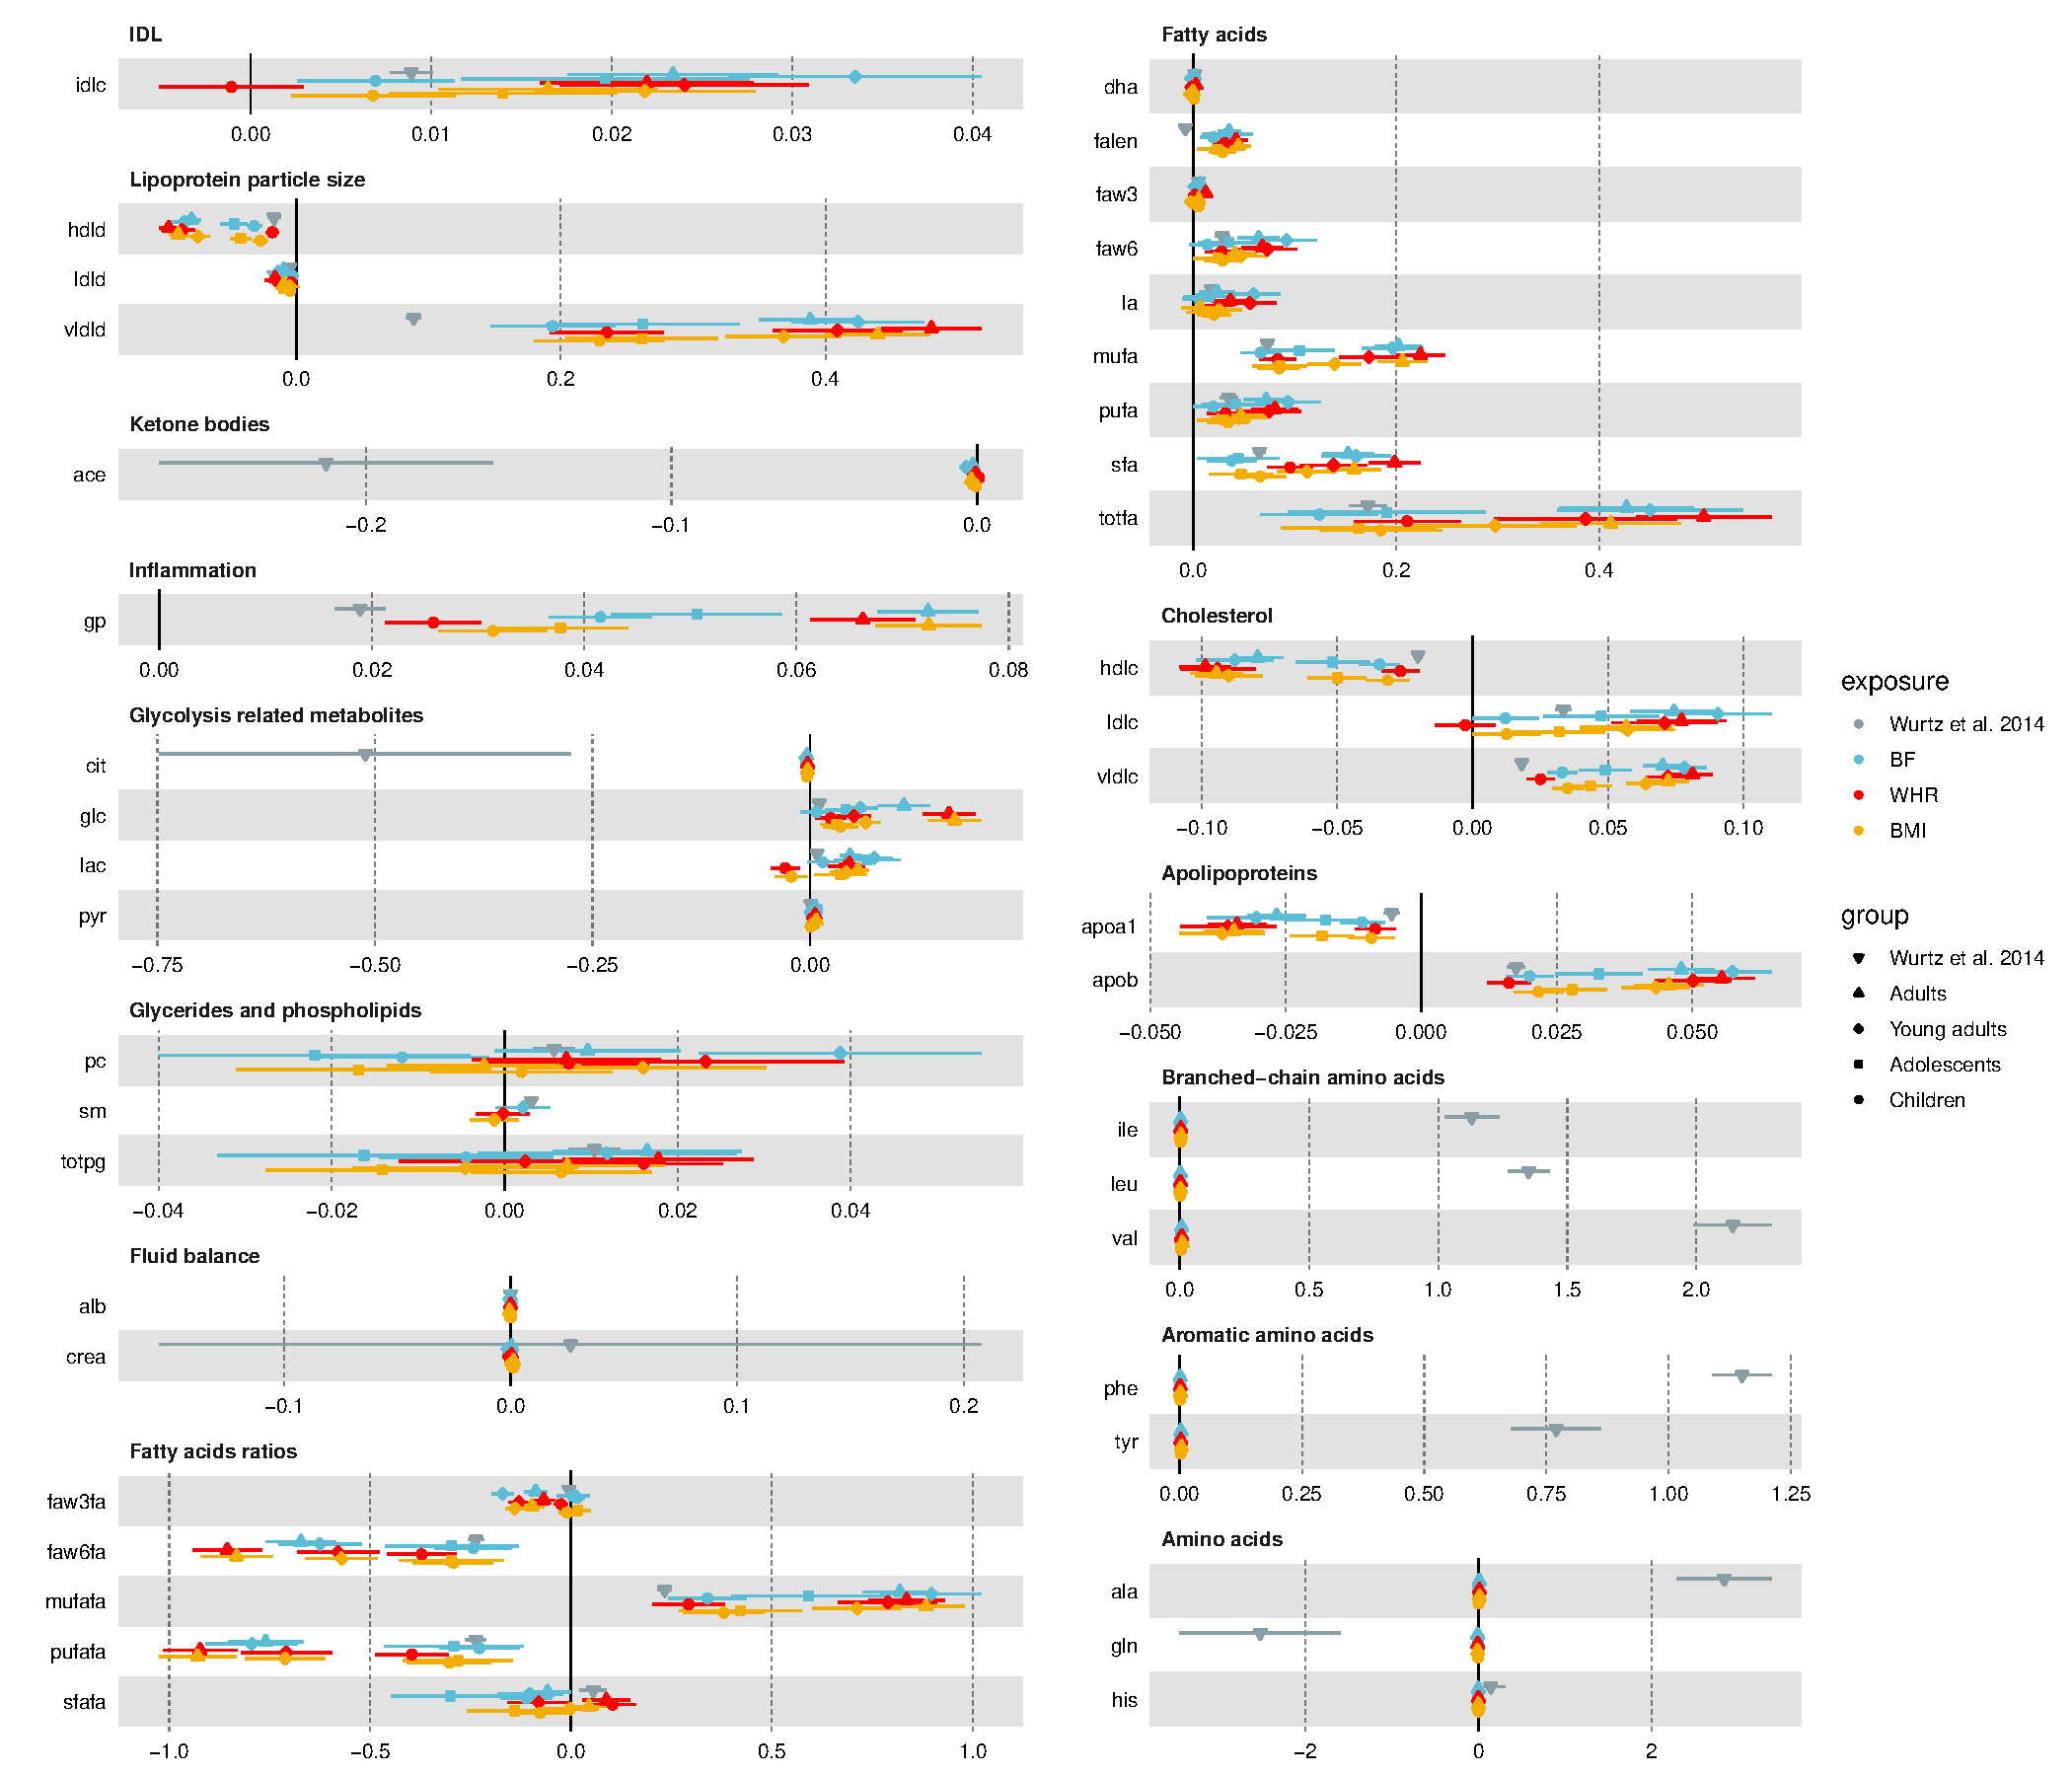
\includegraphics[width=1\linewidth]{data/chapter4/figures/forestplot_wurtz_comparison} \caption{Forestplot of effect estimates across exposures and ages for LDL subclasses}\label{fig:chapter4-figure-forestplot-wurtz-comparison}
\end{figure}
\noindent 
\bsmall
\emph{Figure \ref{fig:chapter4-figure-forestplot-wurtz-comparison} gives the effect estimate and 95\% confidence interval for model 2 across all exposures and age groups.}
\esmall
\elandscape
\newpage

\hypertarget{discussion}{%
\section{Discussion}\label{discussion}}

In this chapter, the influence of increased adiposity on the metabolic profile is demonstrated in an observational framework. These effects persist, not only when measured at different ages, but also when adjusted for confounders and when examined across multiple measures of adiposity.

The association between increased adiposity and metabolites is global, with effects seen across all subclasses of metabolites. These effects are broadly consistent between metabolites within each subclass. When looking at each exposure across age groups (e.g.~the effects of BMI in children, adolescents, young adults, and adults), we find highly similar effects in individuals measured at multiple time points (children, adolescents, and young adults). A similar metabolic profile is apparent in adults, though effect sizes appear slightly larger. The larger effects seen in adults may be due to the fact that metabolite concentrations have been shown to increase in older populations over time\textsuperscript{\protect\hyperlink{ref-Darst2019}{137}}. Given that longitudinal work has shown that BMI tracks over time\textsuperscript{\protect\hyperlink{ref-Singh2008}{165},\protect\hyperlink{ref-Buscot2018}{166}} there may be a dose response relationship here whereby increased adiposity over time leads to increased metabolite concentrations.

Within each age group, there was high directional consistency across the three exposures. Effect sizes across exposures were similar within age groups, with overlapping confidence intervals; BMI showed a broadly higher effect on metabolites across age groups. Effects for BF appeared to be closer to, and crossed, the null more often than BMI and WHR. This may suggest that overall adipose mass in addition to detrimental deposition, may be driving the effect of increased adiposity on metabolites which may lead to disease.

These results are consistent across models; consistency in the direction of effect estimates were observed for the majority of tests. The effect size was broadly similar in the case of models 1 and 2. There was a decreases in effect sizes in model 3 compared with 1 and 2. However, confidence intervals overlapped across the majority of tests even if they crossed the null in some instances for model 3. Consistency across models suggests the association between measures of adiposity and metabolites shows weak evidence of confounding. Whether these results represent a true causal association or are subject to reverse causation or residual confounding requires further investigation.

Previous work by Wurtz et al. (2014)\textsuperscript{\protect\hyperlink{ref-Wurtz2014}{149}} identified numerous associations between BMI and metabolites in a large population. Results here are broadly in line with theirs in terms of effect direction. However, the size of effects differed drastically for a number of metabolites, with much larger effects seen in the study by Wurtz et al(2014)\textsuperscript{\protect\hyperlink{ref-Wurtz2014}{149}}; for the remaining metabolites effect sizes were comparable. These large differences may be a result of differences in metabolite data preparation; here, metabolomics data underwent quality control and if the same quality control had been eprformed by Wurtz et al. (2014)\textsuperscript{\protect\hyperlink{ref-Wurtz2014}{149}} some metabolites may have been excluded. Also, metabolites reported here are absolute values where as Wurtz et al. (2014)\textsuperscript{\protect\hyperlink{ref-Wurtz2014}{149}} scaled concentrations to standard deviation units. In addition, where as multiple covariates were included here, only age and sex were included by Wurtz et al. (2014)\textsuperscript{\protect\hyperlink{ref-Wurtz2014}{149}}. Though effect sizes differed there was consistency in effect direction for key metabolites such as phenylalanine and tyrosine, which, as a result of increased adiposity is increased across ages here and in numerous studies\textsuperscript{\protect\hyperlink{ref-Haufe2016}{167}--\protect\hyperlink{ref-Kim2010b}{174}}.

\hypertarget{limitations}{%
\subsection{Limitations}\label{limitations}}

\hypertarget{metabolomics}{%
\subsubsection{Metabolomics}\label{metabolomics}}

There is no standardised approach, nor a gold standard, for performing metabolomics quality control. Here, quality control, including outlier detection and removal, was performed using the \texttt{MetaboQC} \texttt{R} package. The default settings for exclusions based on metabolite missingness (20\%), sample missingness (20\%), total sum abundance (5 SD), and principal components (5 SD) were used. Most samples were removed for having missingness \textgreater{} 20\% compared to total peak area and PC. Twenty percent sample missingness is arbitrarily defined and used among other studies\textsuperscript{\protect\hyperlink{ref-Lotta2020}{139}}, however a more stringent threshold (e.g.~5\%) may have impacted on results. Especially given that metadata such as batch and runday information was not available. \texttt{MetaboQC} calculated the number of independent metabolites using a clustering dendorgram and a tree cut height based on a Spearman's Rho of 0.5. Although most metabolites were shared across age groups, differences in the number of independent metabolites were found. There were also differences in the number of clusters and truly independent metabolites. Similalry, inclusion of derived metabolites resulted in differing numbers of independent metabolites.

\hypertarget{data-availability}{%
\subsubsection{Data availability}\label{data-availability}}

Metabolomics measures were taken at specific time points in ALSPAC children and at \textasciitilde{}50 years of age in adults. Though measures of adiposity were available at the same time points, data on confounders was not. Smoking status for example was available for adult males at the metabolomics clinic but the closest available measure for adult females was a number of years earlier, in which time they may have taken up smoking. Although data were obtained where available from the closest time point, the mismatch in timings may bias results, particularly in the case of smoking and alcohol consumption.

In all age groups, the availability of data was limiting. Absence of physical activity data meant model 3 was not performed for children, while absence of diet data in young adults and adults meant models 2 and 3 were constrained. However, adjusting for diet where available (children and adolescents) had little impact on results (Table \ref{tab:chapter4-table-significant-results}) and is therefore likely not to have changed findings in young adults and adults.

In children, body fat percentage was not available. A raw impedance measure was available and derivation of BF using Equation \eqref{eq:BF} showed positive correlation with BMI and weight in children and BF measures in adolescents. However, this derived measure included numerous negative estimates of BF. The equation performed well in adolescents, correlating highly with DXA derived BF (Figure \ref{fig:chapter4-figure-BF-validation-correlation-2}). The negative estimates of BF are likely a result of Equation \eqref{eq:BF} being derived in an adult population. Brief investigation showed negative estimates of BF remained when using adolescent age with child height and weight (data not shown). Given that in single frequency devices impedance is based on the volume of an individual it is probable that the values used in the equation do not accurately reflect the proportions of children pre-puberty. Child-specific equations were not available and the manufacturer was unwilling to share the equation used by their impedance devices. However, given that in a linear model the estimate is based on the per-unit increase, the absolute value negative or otherwise, will not impact on the final result.

\hypertarget{sensitivity-analyses}{%
\subsubsection{Sensitivity analyses}\label{sensitivity-analyses}}

The distribution of BMI at each age group was very similar across sexes. However, the distribution of WHR and BF differed among sexes in adolescents, young adults and adults; men had on average a higher WHR while women had a higher BF. Though Z-scores were used and sex was included as a covariate, the differences in WHR and BF distributions may highlight an underlying difference, which confounds the relationship between adiposity and metabolites. For example, hormonal contraceptive use has shown to influence the metabolome\textsuperscript{\protect\hyperlink{ref-Rauschert2017}{175}} and is not regularly taken by individuals with a high BMI\textsuperscript{\protect\hyperlink{ref-Mody2014}{176}}. There was little difference in results from the three models in regards to direction of effect estimates. However, when including only individuals with physical activity (model 3) the size of effects and the number of associations reaching a multiple testing threshold decreased. Given the consistency in the direction of effects across models and the highly similar effects across model 1 and 2 there is likely little effect of confounding. However, the possibility of unmeasured confounding can not be ruled out.

\hypertarget{summary}{%
\subsection{Summary}\label{summary}}

The large number of associations identified using multiple exposures adds weight to the evidence, shown previously for BMI, of association between increased adiposity and metabolites. As with previous work, we find associations between increased adiposity and many metabolites, including increased phenylalanine and tyrosine and decreased HDL components. This work highlights the large effects of increased adiposity on the global metabolic profile and shows that effects likely persist over time. Puberty is likely to have an affect on both adiposity, physical activity, and the metabolome and the lack of available data in children (BF and physical activity) means this requires further investigation, particularly as the adolescent time point used will have included post-pubertal individuals. Though confounders were taken into account the potential for unmeasured confounding is likely, and follow-up analysis will require this to be taken into account. Of particular note is the increasing effect size and number of associations as a result of increased adiposity across the metabolic profile with age. Given that many adiposity associated diseases occur later in life, exposure to an altered metabolic profile over time may be important in disease development, especially as weight loss in overweight and obese individuals is associated with reductions in elevated and increases in reduced metabolites\textsuperscript{\protect\hyperlink{ref-Rangel-Huerta2019}{148}}.

\hypertarget{chapter5}{%
\chapter{Mendelian randomization analysis}\label{chapter5}}

\hypertarget{associations-between-multiple-measures-of-increased-adiposity-and-metabolites-mendelian-randomization-analysis}{%
\subsubsection{\texorpdfstring{\emph{Associations between multiple measures of increased adiposity and metabolites: Mendelian randomization analysis}}{Associations between multiple measures of increased adiposity and metabolites: Mendelian randomization analysis}}\label{associations-between-multiple-measures-of-increased-adiposity-and-metabolites-mendelian-randomization-analysis}}

The large number of associations identified in Chapter \protect\hyperlink{chapter4}{4} and previous observational studies are likely affected by residual confounding. As discussed in Chapter \protect\hyperlink{chapter1}{1}, methods which are somewhat robust to this issue, such as Mendelian randomization, provide an opportunity to further interrogate these associations. Consistent results between observational and Mendelian randomization analyses will strengthen evidence of association between increased adiposity and metabolites and may help to restrict the number of metabolites taken forward for subsequent disease analysis.

\hypertarget{introduction}{%
\section{Introduction}\label{introduction}}

The effects of increased adiposity are observed across the metabolome, with changes in the metabolic profile persisting after correction for measured confounders (Chapter \ref{chapter4}). These persistent effects are similar to previous observational results\textsuperscript{\protect\hyperlink{ref-Wurtz2014}{149}}.

Estimates from observational studies are likely impacted by resuidal confounding. This is also true of models which have been corrected for likely confounders. The effects of residual confounding can lead to larger than expected effect estimates. Bias away from the null is also a factor when reverse causation is present. Mendelian randomization, as discussed in Chapter \ref{chapter1} (\ref{mendelian-randomization}), is able to overcome some of the limitations present with observational studies\textsuperscript{\protect\hyperlink{ref-DaveySmith2003}{80}}.

Work in Chapter \ref{chapter4} is likely not to have fully accounted for confounding, either due to measurement error or unmeasured confounding. For instance, in adults physical activity was measured by questionnaire with possible answeres of `no', `occassionally (less than monthly)' and `frequently (once a month or more)'. Broad categories such as these are unlikely to capture the full impact of physical activity given that `frequently' will encompass individuals who exercie once a month as well as every day. It also does not take into account the intensity of the exercise or its duration. Similar criticism can be placed on the included confounders smoking status and frequency of alcohol consumption. The presene of reverse causation can also not be ruled out. It is possible that metabolic changes promote increased adiposity, though this may be a result of other factors such as diseased states.

With large publicly available GWAS data on metabolites and measures of increased adiposity, here MR is used to examine the causal effect of increased adiposity on the metabolic profile. Particular focus is given to associations which are consistent with those observed in Chapter \ref{chapter1}.

\hypertarget{methods}{%
\section{Methods}\label{methods}}

This chapter details a hypothesis-free two-sample summary-level MR analysis using SNPs for three measures of increased adiposity (BMI, WHR, and BF) measured in individuals of European ancestries as exposures. Outcomes across the three exposures consisted of 123 NMR derived metabolites measured in individuals of European ancestries. The main analysis consisted of an inverse variance weighted multiplicative random effects (IVW-MRE) model and sensitivity analyses using additional models (Figure (\ref{fig:chapter5-figure-schematic}).
\begin{figure}
\includegraphics[width=1\linewidth]{thesis_files/figure-latex/chapter5-figure-schematic-1} \caption{Schematic of Chapter 5 main analysis}\label{fig:chapter5-figure-schematic}
\end{figure}
\noindent 
\bsmall
\emph{The main analysis in chapter 5 included three exposures (BMI (body mass index), WHR (wasit hip ratio), BF (body fat percentage)), 4 models, and 123 metabolite outcomes. The number of SNPs used for each exposure is given alongside the reference for the studies in which the summary data were obtained. The inverse variance weighted, multiplicative random effects model was the main analysis MR Egger, weighted median, and weighted mode are additional sensitivity analyses.}
\esmall

\hypertarget{outcomes-metabolites}{%
\subsection{Outcomes: metabolites}\label{outcomes-metabolites}}

Genome-wide summary level data for 123 NMR derived metabolites (Supplementary Table \ref{tab:appendix-chapter5-table-metabolites}) were obtained from Kettunen et al. (2016)\textsuperscript{\protect\hyperlink{ref-Kettunen2016}{125}} from MR Base\textsuperscript{\protect\hyperlink{ref-Hemani2018}{177}}. Kettunen et al (2016)\textsuperscript{\protect\hyperlink{ref-Kettunen2016}{125}} performed a fixed effects meta-analysis of 123 serum and EDTA serum NMR quantified metabolites from 14 GWASs. In total, up to 24,925 (men = 11,245; women = 13,680) individuals of European ancestries were included in the meta-analysis. A total of 62 SNPs reached a genome wide significance threshold (\emph{p-value} \textless{} 2.27 x 10\textsuperscript{-9}) after correcting for 22 independent tests (22 being the number of principal components explaining over 95\% of variation in the metabolite data). After performing conditional analysis, a further 12 SNPs were identified as independent after reaching the genome-wide significance threshold. The 12 additional SNPs were identified in 9 of the 62 main loci (\emph{PCSK9}, \emph{LPL}, \emph{PPM1K}, \emph{HAL}, \emph{CETP}, \emph{CILP}, \emph{PLTP}, \emph{APOB} and \emph{LIPC}), with a third independent SNP identified in two of these loci (\emph{APOB} and \emph{LIPC}) and a fourth independent SNP identified in one of these (\emph{LIPC}). Overall, 74 independent SNPs were associated with one or more of the 123 metabolites, with the variance explained ranging from 0.2\% for acetoacetate to 12.5\% for glycine, with a median of 5\%.

For the independent GWASs, in each of the 14 cohorts 123 Metabolites were quantified from human blood. Four cohorts used EDTA-plasma, the other 10 used serum. The majority of blood samples were fasted. Where a study did not have over night fasted samples correction for fasting time effect was performed using the \texttt{gam} \texttt{R} package and fitting a smoothed spline to adjust for fasting. The NMR analysis was performed with the comprehensive quantitative serum/plasma platform described by Soininen et al. (2009)\textsuperscript{\protect\hyperlink{ref-Soininen2009}{151}}. All metabolites were first adjusted for age, sex, time from last meal if applicable, and the first ten genomic principal components. The residuals were inverse rank normally transformed. Each of the 14 cohorts performed a univariate GWAS assuming an additive genetic model. SNPs were imputed up to 39 million markers using the 1000 Genomes Project March 2012 version.

For the meta-analysis, SNPs with accurate imputation (info \textgreater{} 0.4) and minor allele count \textgreater{} 3 were combined using double genomic correction, that is, both individual cohort results and meta-analysis results were corrected for the genomic inflation factor as implemented in \texttt{GWAMA}. Up to 12,133,295 SNPs were included in the meta-analysis. Variants, after filtering and meta-analysis, present in more than seven studies were considered for the final results. All traits gave genomic inflation factors in the meta-analysis less than 1.034 showing little evidence of systematic bias in the test statistic.

\hypertarget{exposures-measures-of-increased-adiposity}{%
\subsection{Exposures: measures of increased adiposity}\label{exposures-measures-of-increased-adiposity}}

Genetic instruments were obtained separately for each of three exposures (BMI, WHR, BF). In each case, the following data was obtained: SNP (rsID), effect allele, other allele, effect allele frequency, beta, standard error, \emph{p-value}. F statistics were calculated for each SNP and a mean taken for each exposure -- a nominal threshold of 10 was set.

\hypertarget{body-mass-index}{%
\subsubsection{Body mass index}\label{body-mass-index}}

Genetic instrumental variables for BMI were extracted from Yengo et al. (2018)\textsuperscript{\protect\hyperlink{ref-Yengo2018}{98}}, who analysed data from 515,509 --- 795,624 individuals of European ancestries from two studies, the Genetic Investigation of Anthropometric Traits (GIANT)\textsuperscript{\protect\hyperlink{ref-Locke2015}{96}} and UK Biobank. In both studies BMI was calculated as \(\displaystyle \frac{weight\ (kg)}{height\ (m^2)}\). Yengo et al. (2018)\textsuperscript{\protect\hyperlink{ref-Yengo2018}{98}} performed a fixed effect inverse variance weighted meta-analysis of BMI using GWAS results generated from UK Biobank (N = 456,426) and results from the GIANT consortium, Locek et al. (2015)\textsuperscript{\protect\hyperlink{ref-Locke2015}{96}}.

In UK Biobank, BMI was adjusted for age, sex, recruitment centre, genotyping batch, and the first 10 principal components calculated from 132,102 (out of 147,604) genotyped SNPs pre-selected by the UK Biobank quality control team\textsuperscript{\protect\hyperlink{ref-Bycroft2018}{178}}. In GIANT, BMI was adjusted for age, age squared, and study specific covariates. Both the UK Biobank and GIANT GWASs inverse normally transformed BMI. In total, 681,275 individuals of European ancestry and \textasciitilde{}2.4 million HapMap 2 SNPs were included in the meta-analysis. Linkage disequilibrium score regression (ILDSC 1.03; SE = 0.02) suggested population stratification, however LDSC can rise above 1 as sample sizes and heterogeneity increase\textsuperscript{\protect\hyperlink{ref-Loh2018}{179}}.

In the combined meta-analysis, a total of 656 primary associations reaching a genome wide significance threshold of 5 x 10\textsuperscript{-8} were identified. Approximate conditional and joint multiple-SNP (COJO) analysis identified a further 285 independent SNPs reaching a genome-wide significance threshold (\emph{p-value} \textless{} 1 x 10\textsuperscript{-8}). Together these 941 associations explain 6\% (SE = 0.8\%) and 22.4\% (SE = 3.7\%) of the variance and heritability of BMI respectively. COJO specific summary statistics for all 941 SNPs were used in the main analysis.

\hypertarget{waist-hip-ratio}{%
\subsubsection{Waist hip ratio}\label{waist-hip-ratio}}

Genetic instrumental variables for WHR were extracted from Pulit et al. (2019)\textsuperscript{\protect\hyperlink{ref-Pulit2019}{97}}, who analysed data from 485,486 --- 697,702 individuals of European ancestries from two studies, UK Biobank and GIANT, Shungin et al. (2015)\textsuperscript{\protect\hyperlink{ref-Shungin2015}{95}}. In both studies WHR was calculated as \(\displaystyle \frac{waist\ circumference\ (cm)} {hip\ circumference\ (cm)}\). Pulit et al. (2019)\textsuperscript{\protect\hyperlink{ref-Pulit2019}{97}} performed a fixed effects inverse variance weighted meta-analysis of WHR using GWAS results generated from UK Biobank (N = 485,486 (men = 263,148; women = 222,338)) and results from the GIANT consortium (N = 212,248 (women = 118,004; men = 94,434))\textsuperscript{\protect\hyperlink{ref-Shungin2015}{95}} using METAL\textsuperscript{\protect\hyperlink{ref-Willer2010a}{180}}. SNPs with a frequency difference \textgreater{} 15\% between the two studies were removed prior to meta-analysis. In both studies, WHR was adjusted for sex (UK Biobank only), age at assessment, age at assessment squared and assessment centre (UK Biobank only); study specific covariates were included in the GIANT GWASs where appropriate. All residuals were inverse rank normally transformed; in GIANT residuals were calculated for men and women separately. In total, 316 associations reaching a genome wide significance threshold of 5 x 10\textsuperscript{-9} were identified; \emph{p-value} adjusted to account for denser imputation data\textsuperscript{\protect\hyperlink{ref-Pulit2017a}{181}}. These associations explain 3\% of the phenotypic variance as calculated in an independent dataset (N = 7,721). SNP based heritability across all SNPs was estimated to be 22.7\%.

For the UK Biobank GWAS the second release (June 2017) of UK Biobank data which did not have corrected imputation at non-HRC sites was used. As such, only HRC SNPs were used in the GWAS. A linear mixed model using BOLT-LMM\textsuperscript{\protect\hyperlink{ref-Loh2015}{182}} was performed on SNPs with imputation quality score \textgreater{} 0.3, MAF \textgreater{} 0.01\% and SNPs present in the HRC imputation reference panel. Adjustment was made for the SNP array used to genotype the sample. No other covariates were used. They did not assume a non-infinitesimal model. In GIANT, individual studies (genome-wide array = 57; Metabochip = 44) recruited participants and undertook sample and SNP quality control. In genome-wide array studies, imputation was performed with CEU haplotypes from HapMap. Assuming an additive genetic model, each study ran a linear regression GWAS. Sex-specific summary statistics were corrected for population structure using the genomic control inflation factor. Prior to meta-analysis of genome-wide array studies and Metabochip studies, SNPs were removed if they had a minor allele count \textless{}= 3, were not in Hardy-Weinberg equilibrium (\emph{p-value} \textless{} 10\textsuperscript{-6}), had a call rate \textless{} 95\% or an imputation quality score \textless{} 0.3 for MACH, 0.4 for IMPUTE, and 0.8 for PLINK. A fixed effects inverse variance weighted meta-analysis of each genome-wide array GWAS and each Metabochip GWAS was performed and corrected for genomic control to account for structure between cohorts. A fixed effects inverse variance weighted meta-analysis of the meta-analysed genome-wide array studies and Metabochip studies was performed using METAL; correction for genomic control was not performed.

\hypertarget{body-fat-percentage}{%
\subsubsection{Body fat percentage}\label{body-fat-percentage}}

Genetic instrumental variables for BF were extracted from Lu et al. (2016)\textsuperscript{\protect\hyperlink{ref-Lu2016}{183}}. This was the only available GWAS using DXA as a measure of BF (as of 25/07/2019); the number of individuals with DXA measures was not reported. Lu et al. (2016)\textsuperscript{\protect\hyperlink{ref-Lu2016}{183}} performed a fixed effects inverse variance weighted meta-analysis of BF using two meta-analyses generated from 43 GWASs (N = 65,831) and 13 Metabochip GWAS studies (N = 23,468) using METAL\textsuperscript{\protect\hyperlink{ref-Willer2010a}{180}}. In total, up to 89,300 (men = 44,429; women = 45,525) individuals of European ancestries were included in the inverse variance weighted fixed effects meta-analysis. In total 7 SNPs reached a genome wide significance threshold (\emph{p-value} \textless{} 5 x 10-8) and were considered independent (± 500kb of the most significant SNP). Estimation of variance explained was not available in the European ancestries meta-analysis. In the all ancestries meta-analysis, which included up to 11,419 additional individuals of non-European ancestries, these 7 SNPs explained 0.416\% of the variance in BF -- additional SNPs identified in the all ancestries meta-analysis explained 0.58\% of the variance in BF.

In each cohort, BF was measured via a bioletrical impedance device or DXA as described previously\textsuperscript{\protect\hyperlink{ref-Kilpelainen2011b}{184}}. For each study, BF was adjusted for age, age squared and study-specific covariates (e.g.~genotype-based principle components and study centre), if necessary. For studies of unrelated individuals, the residuals were calculated separately in men and women, and in cases and controls. For studies of family-based design, the residuals were calculated in men and women together, and sex was additionally adjusted in the model. The residuals were then inverse rank normally transformed for association testing. For studies of family-based design, the family relatedness was additionally adjusted in the association testing.

Meta-analysis was performed in two stages. First, two parallel meta-analyses were conducted; one meta-analysis combined summary statistics from 43 GWASs, totalling up to 65,831 individuals of European ancestries and the other meta-analysis combined summary statistics from 13 Metabochip studies, totalling up to 23,469 individuals of European ancestries. Each study performed study specific quality control. Imputation was performed in each study using the European ancestries HapMap Phase II (Release 22) reference panel. Individual SNPs were associated with inverse normally transformed BF residuals using linear regression with an additive model. All SNPs with low imputation scores (MACH r2-hat \textless{} 0.3, IMPUTE proper\_info \textless{} 0.4, or PLINK info \textless{} 0.8) and a MAC \textless{}= 3 were removed. The \texttt{EasyQC} software was used for detailed QC of study level analyses and meta-level analysis.

In the second stage, a single meta-analysis of the GWAS meta-analysis results and the Metabochip meta-analysis results was performed. This included up to 89,300 individuals of European ancestries from 56 studies. Meta-analysis was performed using an inverse variance-weighted fixed-effect method using METAL. Inflation before genomic control correction was generally low (lambda men + women = 1.13; lambda men = 1.07; lambda women = 1.10). To reduce inflation of test statistics from potential population structure, individual GWAS results and GWAS meta-analysis results were corrected for genomic control using all SNPs. Individual Metabochip results and Metabochip meta-analysis results were genomic control corrected using 4,425 SNPs, which were derived from pruning of QT-interval replication SNPs within 500 kb of an anthropometry replication SNP on the Metabochip. The genomic control corrected GWAS and Metabochip meta-analysis results were then meta-analysed.

LDSC suggested observed inflation was not due to population substructure; the regression intercept was 1.0045 (lambda genomic control = 1.136 and mean X2 = 1.16) for sex-combined, 0.999 (lambda genomic control = 1.062 and mean X2 = 1.079) for men-only and 1.014 (lambda genomic control = 1.105 and mean X2 = 1.112) for women-only analyses. The authors used these regression intercepts, rather than the lambda genomic control, to correct the meta-analysis results in more significant associations (for example, for the rs1558902-\emph{FTO} SNP, \emph{p-value} = 3.24 x 10-27 in the modified European sex-combined meta-analysis compared with \emph{p-value} = 1.1 x 10-25). Overall, the less stringent correction did not result in the identification of novel loci.

Each unique locus was defined as ±500\emph{kb} on either side of the most significant SNP that reached the genome wide significance threshold (\emph{p-value} \textless{} 5 x 10-8) in the meta-analysis. Genotype data for genome-wide significant SNPs was of high quality with a median imputation score of \textgreater{}= 0.95. The fifth percentile for all SNPs was \textgreater{}= 0.80, except for the previously established \emph{TOMM40} SNP (P5 = 0.52).

\hypertarget{statistical-analysis}{%
\subsection{Statistical analysis}\label{statistical-analysis}}

All data manipulation and analysss was perfromed using \texttt{R}\textsuperscript{\protect\hyperlink{ref-r2019}{146}} (version 3.5.3). MR analysis was performed using the \texttt{TwoSampleMR}\textsuperscript{\protect\hyperlink{ref-Hemani2018}{177}} (version 0.4.22) \texttt{R} package. Data on metabolites were obtained from MR Base (accessed 26/07/2019).

For all exposures, the following data were obtained from the original GWAS publications: rsID, effect allele, other/non-effect allele, effect allele frequency, effect estimate, standard error of the effect estimate, \emph{p-value}, N, and units. The same data for these genetic instrumental variables were obtained from each metabolite for each exposure separately. Where genetic instrumental variables were not present in the metabolite GWASs, proxy SNPs were included if linkage disequilibrium was \textgreater{}= 0.8. For proxy SNPs, the inclusion of SNPs where the reference strand was ambiguous (strand flips) was allowed and the direction was inferred using a minor allele frequency threshold of 0.3.

Exposure and outcome SNPs were harmonized in reference to the exposure effect allele being on the increasing scale. For included alleles where the reference strand was ambiguous, the positive strand was inferred using effect allele frequency.

\hypertarget{main-analysis}{%
\subsubsection{Main analysis}\label{main-analysis}}

An inverse variance weighted (IVW), multiplicative random effects (IVW-MRE) model was used to investigate the causal association of each exposure on each metabolite. The model assumes that the strength of the association of the genetic instruments with the exposure is not correlated with the magnitude of the pleiotropic effects and that the pleiotropic effects have an average value of zero\textsuperscript{\protect\hyperlink{ref-Bowden2017}{185}}. A multiple testing threshold of \emph{p-value} \textless{} 0.0022727 was used. This is based on the number of principal components (22) in the Kettunen et al. (2016)\textsuperscript{\protect\hyperlink{ref-Kettunen2016}{125}} meta-analysis that explained 95\% of the variation in metabolite data. Consistency in the direction of effect estimates was investigated and Spearman's Rho analysis of effect estimates was performed.

For the main analysis, results represent the change in the inverse rank position of each metabolite per change in the inverse rank position of the exposure.

\hypertarget{sensitivity-analysis}{%
\subsubsection{Sensitivity analysis}\label{sensitivity-analysis}}

Assumptions of no pleiotropy among genetic instruments and outcomes were explored using MR-Egger\textsuperscript{\protect\hyperlink{ref-Bowden2015a}{186}}, weighted median\textsuperscript{\protect\hyperlink{ref-Burgess2017a}{187}} and weighted mode\textsuperscript{\protect\hyperlink{ref-Hartwig2017}{188}} based estimators, which are sensitive to the effects of potential pleiotropy. No threshold requirements were set for these methods, instead consistency between the IVW-MRE model and these methods was investigated.

MR-Egger provides an estimate of horizontal pleiotropy via the intercept of a linear regression of the SNP-exposure and SNP-outcome association. Absent pleiotropic effects the intercept tends towards the origin. MR-Egger gives consistent estimates when 100\% of genetic instruments are invalid\textsuperscript{\protect\hyperlink{ref-Bowden2015a}{186}}. The weighted median is complimentary to MR-Egger but does not rely on the instrument strength independent of direct effect assumption. It calculates the median of an empirical distribution of effect estimates weighted for precision. It provides consistent estimates when at least 50\% of the weight comes from genetic instruments and as long as no one genetic instrument contributes \textgreater{} 50\% of the weight\textsuperscript{\protect\hyperlink{ref-Burgess2017a}{187}}. The weighted mode assumes the true causal effect is the most common effect. It relies on the assumption that across all instruments the mode is 0\textsuperscript{\protect\hyperlink{ref-Hartwig2017}{188}}.

The effects of heterogeniety in the exposure instruments was investigated using Cochrane's Q statistic for maximum likelihood, IVW, and MR Egger models. A single SNP MR, whereby the causal association of each SNP individually is estimated using the maximum likelihood and Wald ratio models, was also used to investigate heterogeneity. A leave-one-out MR analysis was performed whereby each SNP is sequentially left out of the MR analysis and the causal effect estimated absent of that SNP. If the estimated effect is substantially reduced after the removal of a single SNP this may imply violation of the exclusion restriction assumption and that this SNP is having a direct association with the outcome that is not mediated through the exposure. Finally, each of these additional sensitivity analyses were visualised using a funnel plot of the instrument beta and standard error and using forest plots of the single SNP and leave-one-out MR analysis to identify potential pleiotropic effects. Additional sensitivity analysis is presented as a summary for each exposure. Where appropriate, i.e.~for results which appear to be strong associations, specific results are discussed.

\hypertarget{additional-analyses}{%
\subsection{Additional analyses}\label{additional-analyses}}

In the main analysis both BMI and WHR genetic instrumental variables were obtained from studies using UK Biobank, which has shown evidence of latent population structure\textsuperscript{\protect\hyperlink{ref-Haworth2019}{89},\protect\hyperlink{ref-Berg2019}{90}} (See \ref{mendelian-randomization}). Additionally, BMI instruments were obtained from a COJO analysis, which, as these SNPs are conditional on the presence of an independent SNP, may lead to potential pleiotropic pathways. Finally, BF instruments were obtained from a study which used different measures of BF; two of the included SNPs have also been associated previously with `favourable adiposity' and may therefore not be reflections of total body fat\textsuperscript{\protect\hyperlink{ref-Yaghootkar2014}{189},\protect\hyperlink{ref-Yaghootkar2016}{190}}. In order to test whether genetic instrumental variables in the main analysis produced biased results a two step additional analysis was performed.

Firstly, genetic instrumental variables for BMI, WHR and BF were obtained from additional sources (Supplementary Table \ref{tab:appendix-chapter5-table-exposures}). Outcome data extraction and harmonization was performed as for the main analysis. F statistics and detailed information on each additional exposure is available in Supplementary information. Briefly, SNPs for BMI were obtained from the initial non-COJO analysis by Yengo et al 2018\textsuperscript{\protect\hyperlink{ref-Yengo2018}{98}}, and a separate set of SNPs were obtained from Locke et al. (2015)\textsuperscript{\protect\hyperlink{ref-Locke2015}{96}} which did not use UK Biobank; for WHR, SNPs were obtained from Shungin et al. (2015)\textsuperscript{\protect\hyperlink{ref-Shungin2015}{95}} which did not use UK Biobank; for BF, the SNPs associated with `favourable adiposity' were removed and an additional SNP set identified in a GWAS using a single measure of BF was obtained from Hubel et al. (2019)\textsuperscript{\protect\hyperlink{ref-Hubel2019}{191}}.

In stage one, the main analysis (IVW-MRE, MR-Egger, Weighted median, Weighted mode and additional sensitivity analysis) was performed using these additional exposures. In stage two, genetic instrumental variables for all exposures (those used in the main analysis and in additional analyses described here) were clumped and the main analysis was performed. Clumping was performed using the \texttt{R} package \texttt{TwoSampleMR}\textsuperscript{\protect\hyperlink{ref-Hemani2018}{177}} (version 0.4.22) setting a linkage disequilibrium R\textsuperscript{2} threshold of \(0.001\) for SNPs within a 10,000 base window of each other. Spearman's Correlation between MR results from the non-clumped and clumped SNP lists was performed.

\hypertarget{comparison-with-observational-estimates}{%
\subsection{Comparison with observational estimates}\label{comparison-with-observational-estimates}}

Finally, comparison of results here and those from observational analysis conducted in Chapter \ref{chapter4} was performed. Observational estimates from the adult analysis, adjusted for age and sex, were used along with those of the main analysis here. Firstly, consistency in the direction of effect within exposures across MR and observational estimates was investigated, and a Spearmans Rho analysis was performed. Secondly, tests reaching a multiple testing threshold across both observational and MR analyses within exposures were investigated. Finally, tests which showed consistency in direction of effect and which reached a multiple testing threshold across analyses and exposures were investigated.

\hypertarget{comparison-with-wurtz-et-al.-2014wurtz2014}{%
\subsection{\texorpdfstring{Comparison with Wurtz et al. (2014)\textsuperscript{\protect\hyperlink{ref-Wurtz2014}{149}}}{Comparison with Wurtz et al. (2014)149}}\label{comparison-with-wurtz-et-al.-2014wurtz2014}}

\hypertarget{results}{%
\section{Results}\label{results}}

\hypertarget{main-analysis-f-statistics}{%
\subsection{Main analysis F-statistics}\label{main-analysis-f-statistics}}

Numerous SNPs were used for each exposure in the main analysis. For each SNP an F-statistic was calculated and a mean taken for each exposure. Across all three exposures, no single SNP had an F-statistic less than 10. Mean F-statistics: BMI = 73, WHR = 66, BF = 44 (Figure \ref{fig:chapter5-figure-fstat-main}).
\begin{figure}
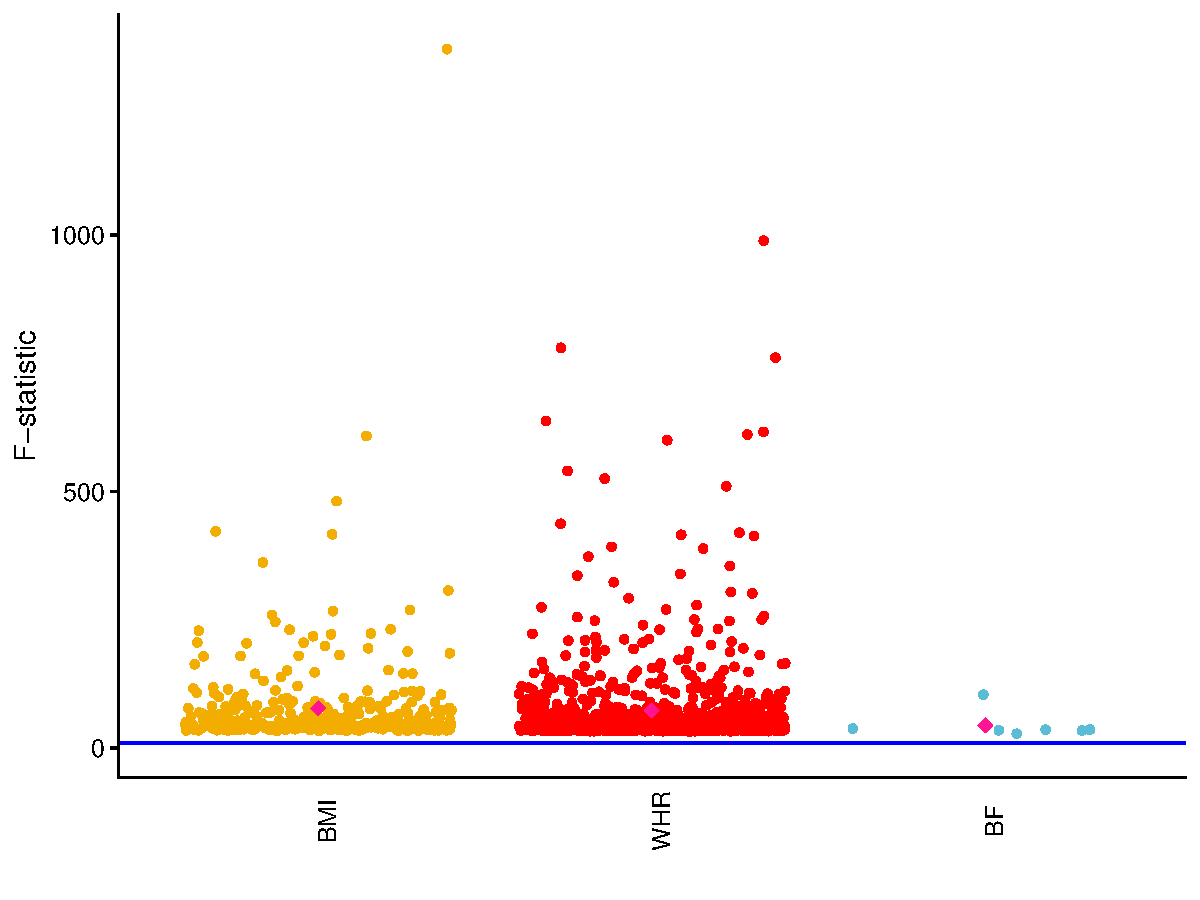
\includegraphics[width=1\linewidth]{../../002_adiposity_metabolites/analysis/main_exposures_fstatistics} \caption{Main MR analysis f-statistics}\label{fig:chapter5-figure-fstat-main}
\end{figure}
\noindent 
\bsmall
\emph{Mean f-statistics for each exposure indicated by the pink diamond. The blue line indicates a nominal threshold of 10. BMI = body mass index, WHR = wasit hip ratio, BF = body fat percentage.}
\esmall

\hypertarget{statistical-analysis-1}{%
\subsection{Statistical analysis}\label{statistical-analysis-1}}

\hypertarget{main-analysis-1}{%
\subsubsection{Main analysis}\label{main-analysis-1}}

\hypertarget{directional-consistency}{%
\paragraph{Directional consistency}\label{directional-consistency}}

Across all three exposures, directional consistency was low (Figure \ref{fig:chapter5-figure-directional-consistency}), with over 100 of the 123 tests showing an opposite direction of effect for at least one exposure. Consistency in the direction of effect was highest for BMI and WHR, where a mjority of tests showed positive effects. Directional inconsistency was largely due to BF having an opposite direction of effect on metabolites to BMI and WHR. Spearman's Rho analysis of effect estimates showed a positive correlation between BMI and WHR (R\textsuperscript{2} = 0.94), while negative correlations were observed for BF and BMI (R\textsuperscript{2} = -0.70) and BF and WHR (R\textsuperscript{2} = -0.72) (Supplement \ref{chapter4-appendix-correlations}).
\begin{figure}
\includegraphics[width=1\linewidth]{thesis_files/figure-latex/chapter5-figure-directional-consistency-1} \caption{Directional consistency across exposures}\label{fig:chapter5-figure-directional-consistency}
\end{figure}
\noindent 
\bsmall
\emph{Figure \ref{fig:chapter5-figure-directional-consistency} shows the directional consistency of all exposures from the main analysis: BMI (Yengo et al. (2018)), WHR (Pulit et al. (2018)), BF (Lu et al. (2016)). A positive effect reflects the effect estimate from two or more exposures being in the positive direction; a negative effect reflects betas being in a negative direction; opposite effect reflects different directions for the effect estimates. BMI = body mass index; WHR = waist hip ratio; BF = body fat percentage.}
\esmall

\hypertarget{multiple-testing-threshold}{%
\paragraph{Multiple testing threshold}\label{multiple-testing-threshold}}

A total of 63, 63, and 0 tests reached a multiple testing threshold for BMI, WHR and BF respectively. Of these tests, 58 reached a multiple testing threshold across both BMI and WHR. A total of 5 and 5 tests reached a multiple testing threshold for BMI only and WHR only respectively. For BMI, these metabolites included, Acetate (mmol/l), Average number of methylene groups per double bond, Concentration of IDL particles (mol/l), Monounsaturated fatty acids; 16:1, 18:1 (mmol/l), Phospholipids in very small VLDL (mmol/l); for WHR, these metabolites included, Glutamine (mmol/l), Lactate (mmol/l), Concentration of small HDL particles (mol/l), Total cholesterol in very large HDL (mmol/l), Cholesterol esters in very large HDL (mmol/l).

Given no tests reached a multiple testing threshold for BF, focus here is on the tests reaching a multiple testing threshold across both BMI and WHR. All tests reaching the multiple testing threshold for BMI and WHR where directionally consistent across BMI and WHR (Figure \ref{fig:chapter5-figure-threshold-directional-consistency}). Of the tests which reached a multiple testing threshold across BMI and WHR, 4 were directionally consistent across BMI, WHR and BF, with positive effect estimates for: Phenylalanine (mmol/l), Tyrosine (mmol/l), Valine (mmol/l); and negetive effect estimates for Apolipoprotein A-I (g/l) (Figure \ref{fig:chapter5-figure-forestplot-associations}. Effect sizes were broadly consistent across BMI and WHR; BF had much larger confidence intervals which spanned the null.
\begin{figure}
\includegraphics[width=1\linewidth]{thesis_files/figure-latex/chapter5-figure-threshold-directional-consistency-1} \caption{Directional consistency across exposures for tests reahcing a multiple testing threshold}\label{fig:chapter5-figure-threshold-directional-consistency}
\end{figure}
\noindent 
\bsmall
\emph{Figure \ref{fig:chapter5-figure-threshold-directional-consistency} shows the directional consistency of all exposures from the main analysis which reached a multiple testing threshold (p \textless{} 0.05/22): BMI (Yengo et al. (2018)), WHR (Pulit et al. (2018)), BF (Lu et al. (2016)). A positive effect reflects the effect estimate from two or more exposures being in the positive direction; a negative effect reflects betas being in a negative direction; opposite effect reflects different directions for the effect estimates. BMI = body mass index; WHR = waist hip ratio; BF = body fat percentage.}
\esmall
\begin{figure}
\includegraphics[width=1\linewidth]{thesis_files/figure-latex/chapter5-figure-forestplot-associations-1} \caption{Forestplot of directionally consistent tests reaching a multiple testing threshold}\label{fig:chapter5-figure-forestplot-associations}
\end{figure}
\noindent 
\bsmall
\emph{Figure \ref{fig:chapter5-figure-forestplot-associations} shows effect estimates and 95\% confidence intervals for the 4 metabolites which reached a multiple testing threshold (p \textless{} 0.05/22) for BMI and WHR and which where directionally consistent across all 3 exposures: BMI (Yengo et al. (2018)), WHR (Pulit et al. (2018)), BF (Lu et al. (2016)). Effect estimates represent the change in the inverse rank position of each metabolite per change in the inverse rank position of the exposure.}
\esmall

\hypertarget{global-metabolic-profile}{%
\paragraph{Global metabolic profile}\label{global-metabolic-profile}}

Globally, the pattern of association was visually very similar for BMI and WHR. Effects for WHR were generally larger with wider confidence intervals, whereas those for BMI where smaller with tighter confidnece intervals. Effects for BF were much larger with wide confidence intervals which spanned the null (Figure \ref{fig:chapter5-figure-circosplot-main-analysis}). The largest negative effects (\(> -0.75\)) were found for BF and the Total lipis and Particle concentration metabolites within the \emph{Small LDL}, \emph{Small VLDL}, and \emph{Medium LDL} subclasses. The largest positive effects (\(> 0.40\)) were observed for BF and the \emph{Medium HDL} and \emph{Large HDL} subclasses. All metabolites in subclasses \emph{Small VLDL}, \emph{Medium VLDL}, \emph{Large VLDL}, \emph{Very large VLDL}, \emph{Extremely large VLDL}, \emph{Large HDL}, \emph{Apolipoproteins}, \emph{Branched-chain amino acids}, and \emph{Aromatic amino acids} reached the multiple testing threshold across both BMI and WHR. In addition, metabolites in these subclasses all shared the same direction of effect with other metabolites within their respective subclass for both BMI and WHR.
\begin{figure}
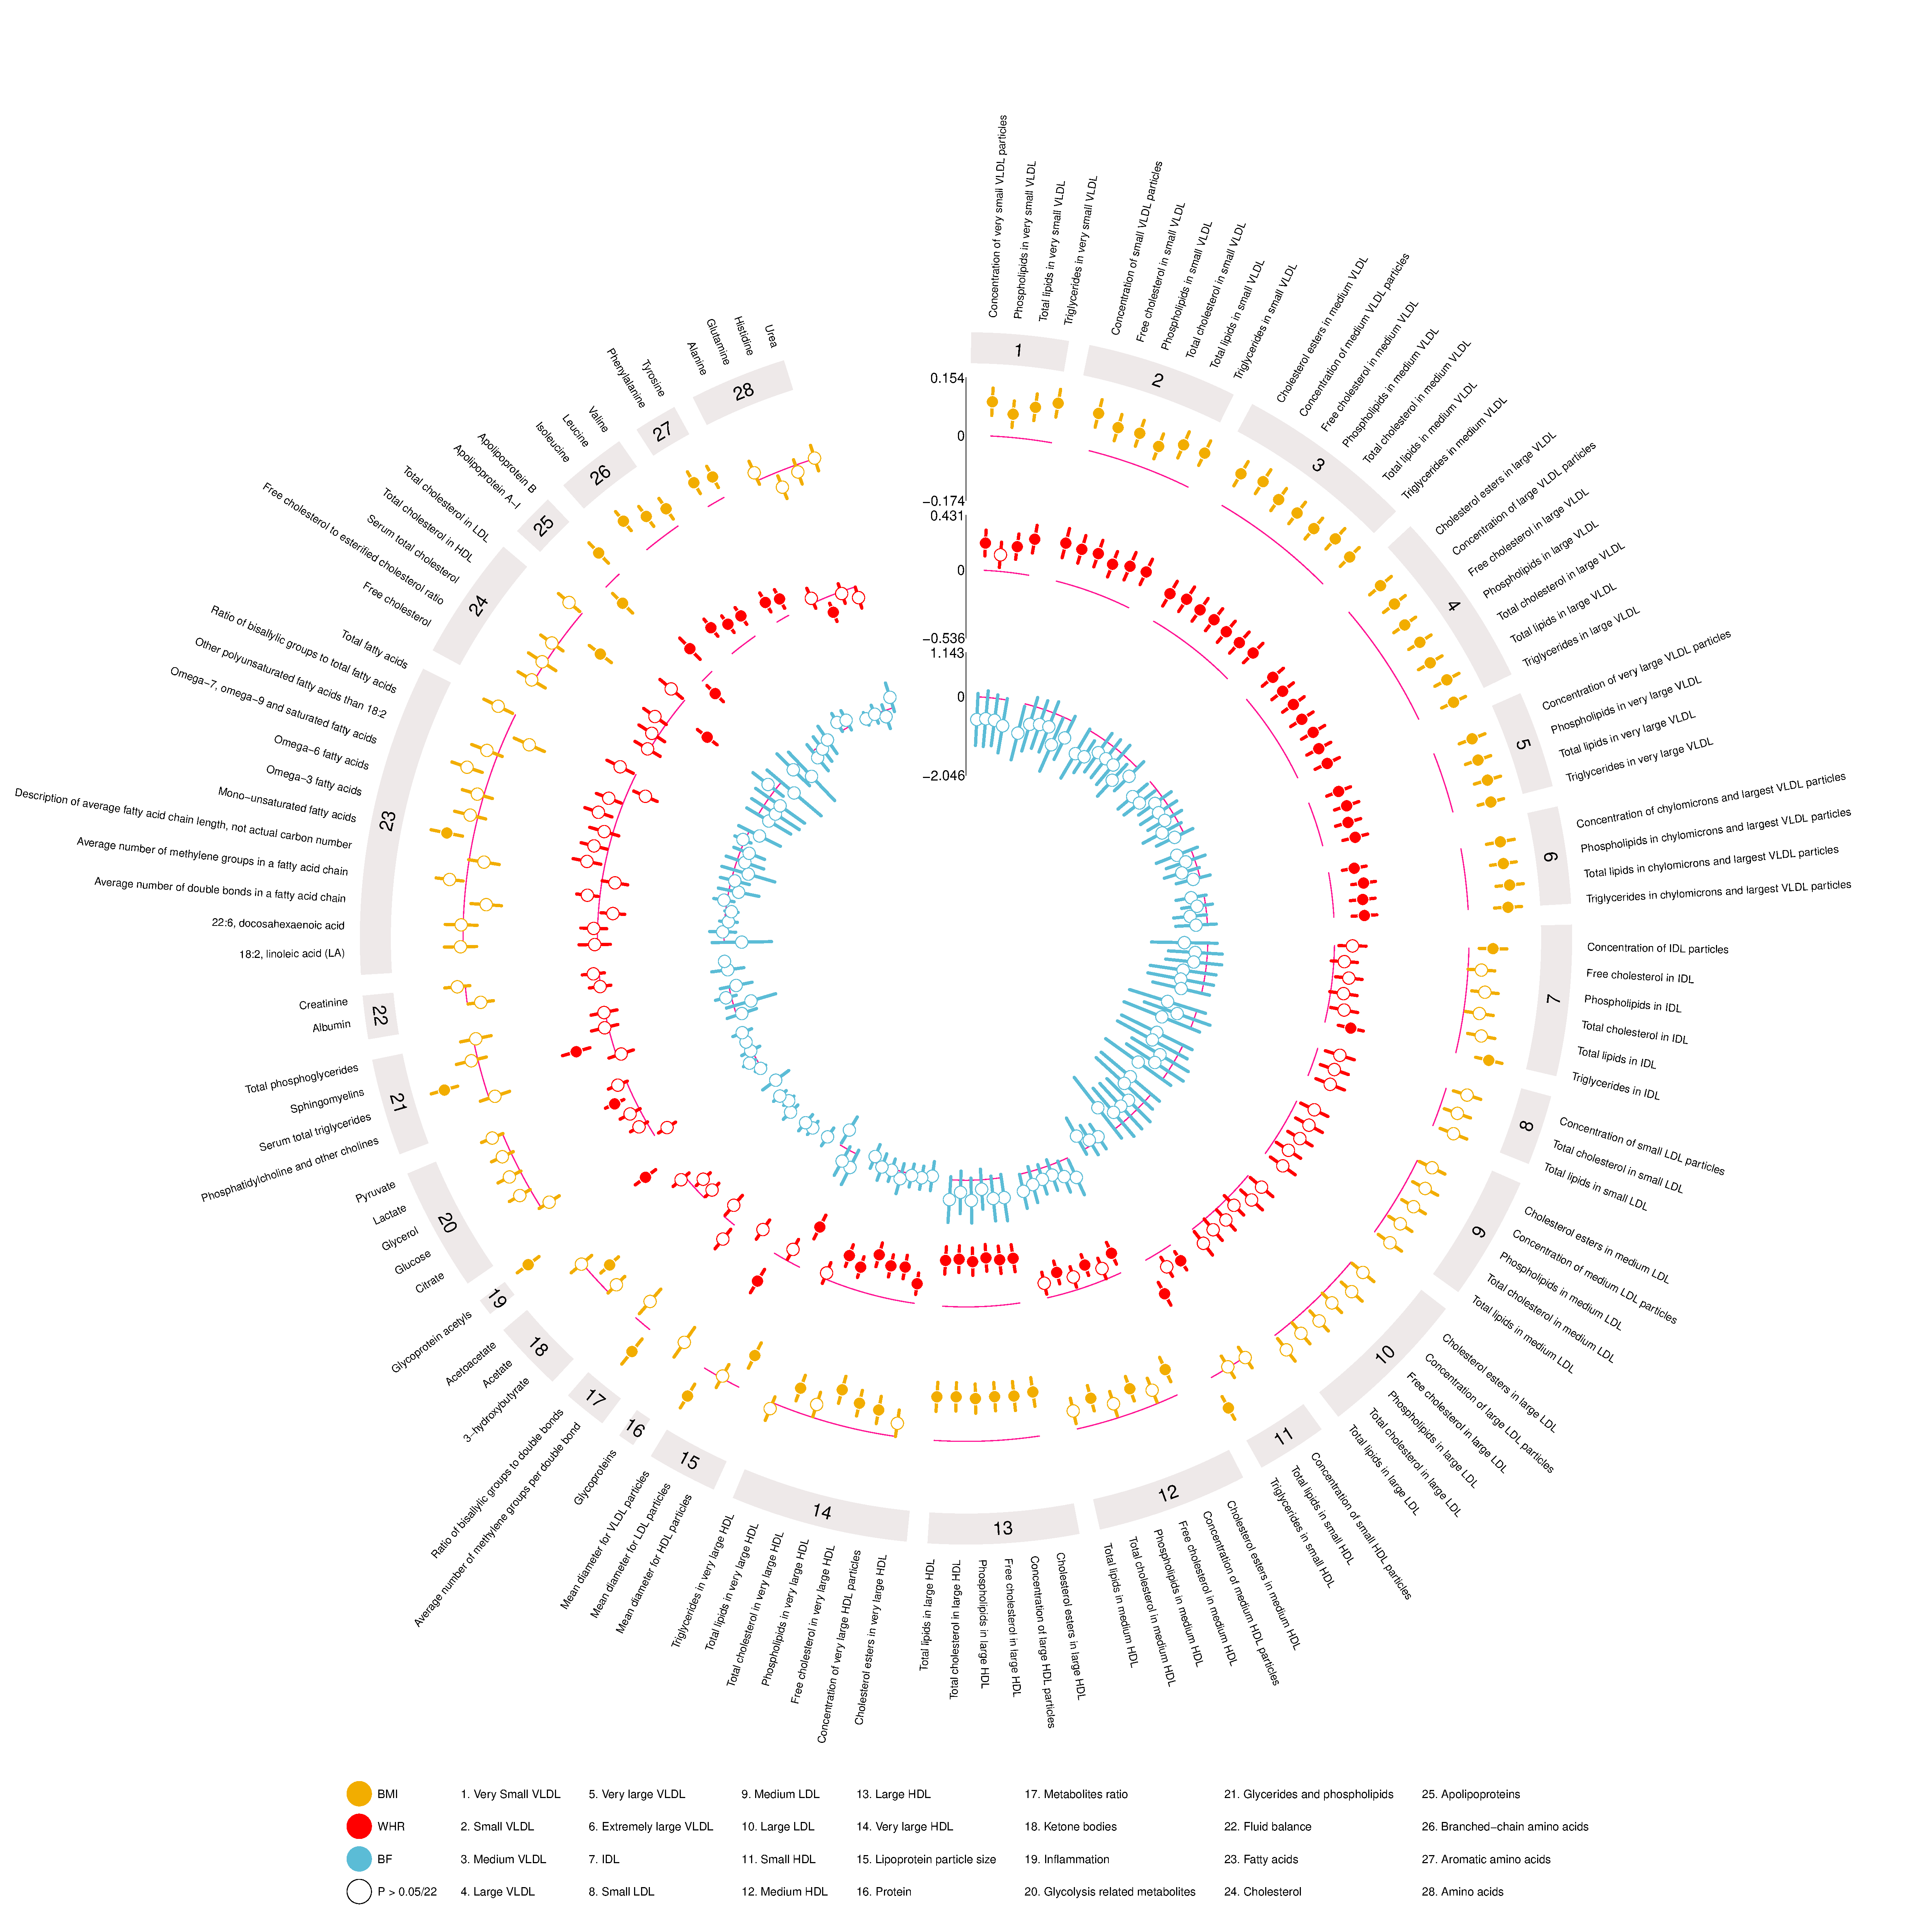
\includegraphics[width=1\linewidth]{data/chapter5/figures/circosplot_main_analysis} \caption{Circos plot of IVW-MRE effect estimates for BMI, WHR, and BF on 123 NRM derived metabolites}\label{fig:chapter5-figure-circosplot-main-analysis}
\end{figure}
\noindent 
\bsmall
\emph{Figure \ref{fig:chapter5-figure-circosplot-main-analysis} shows each track as one of the measures of increased adiposity; the outer track is BMI, the middle track is WHR, the inner track is BF. Solid points indicate a multiple testing threshold (\(0.05/22\)) has been reached. Effect estimates represent the change in the inverse rank position of each metabolite per change in the inverse rank position of the exposure. 95\% confidence intervals shown. Metabolites are grouped by subclass.}
\esmall

\hypertarget{subclass-results}{%
\paragraph{Subclass results}\label{subclass-results}}

Tests reaching the multiple testing threshold were observed for at least one exposure in 23 of 28 subclasses. No tests reached a multiple testing threshold for subclasses: \emph{Small LDL}, \emph{Medium LDL}, \emph{Large LDL}, \emph{Protein}, \emph{Fluid balance}. For subclasses \emph{IDL}, \emph{Metabolites ratio}, \emph{Ketone bodies}, \emph{Glycolysis related metabolites}, \emph{Glycerides and phospholipids}, \emph{Cholesterol}, and \emph{Amino acids} only a small number of metabolites within each subclass reached the multiple testing threshold. Whereas, for subclasses \emph{Small VLDL}, \emph{Medium VLDL}, \emph{Large VLDL}, \emph{Very large VLDL}, \emph{Extremely large VLDL}, \emph{Large HDL}, \emph{Very large HDL}, \emph{Lipoprotein particle size}, \emph{Branched-chain amino acids}, and \emph{Aromatic amino acids} a majority of metabolites reached the multiple testing threshold (Figure \ref{fig:chapter5-figure-forestplot-subclasses}).
\begin{figure}
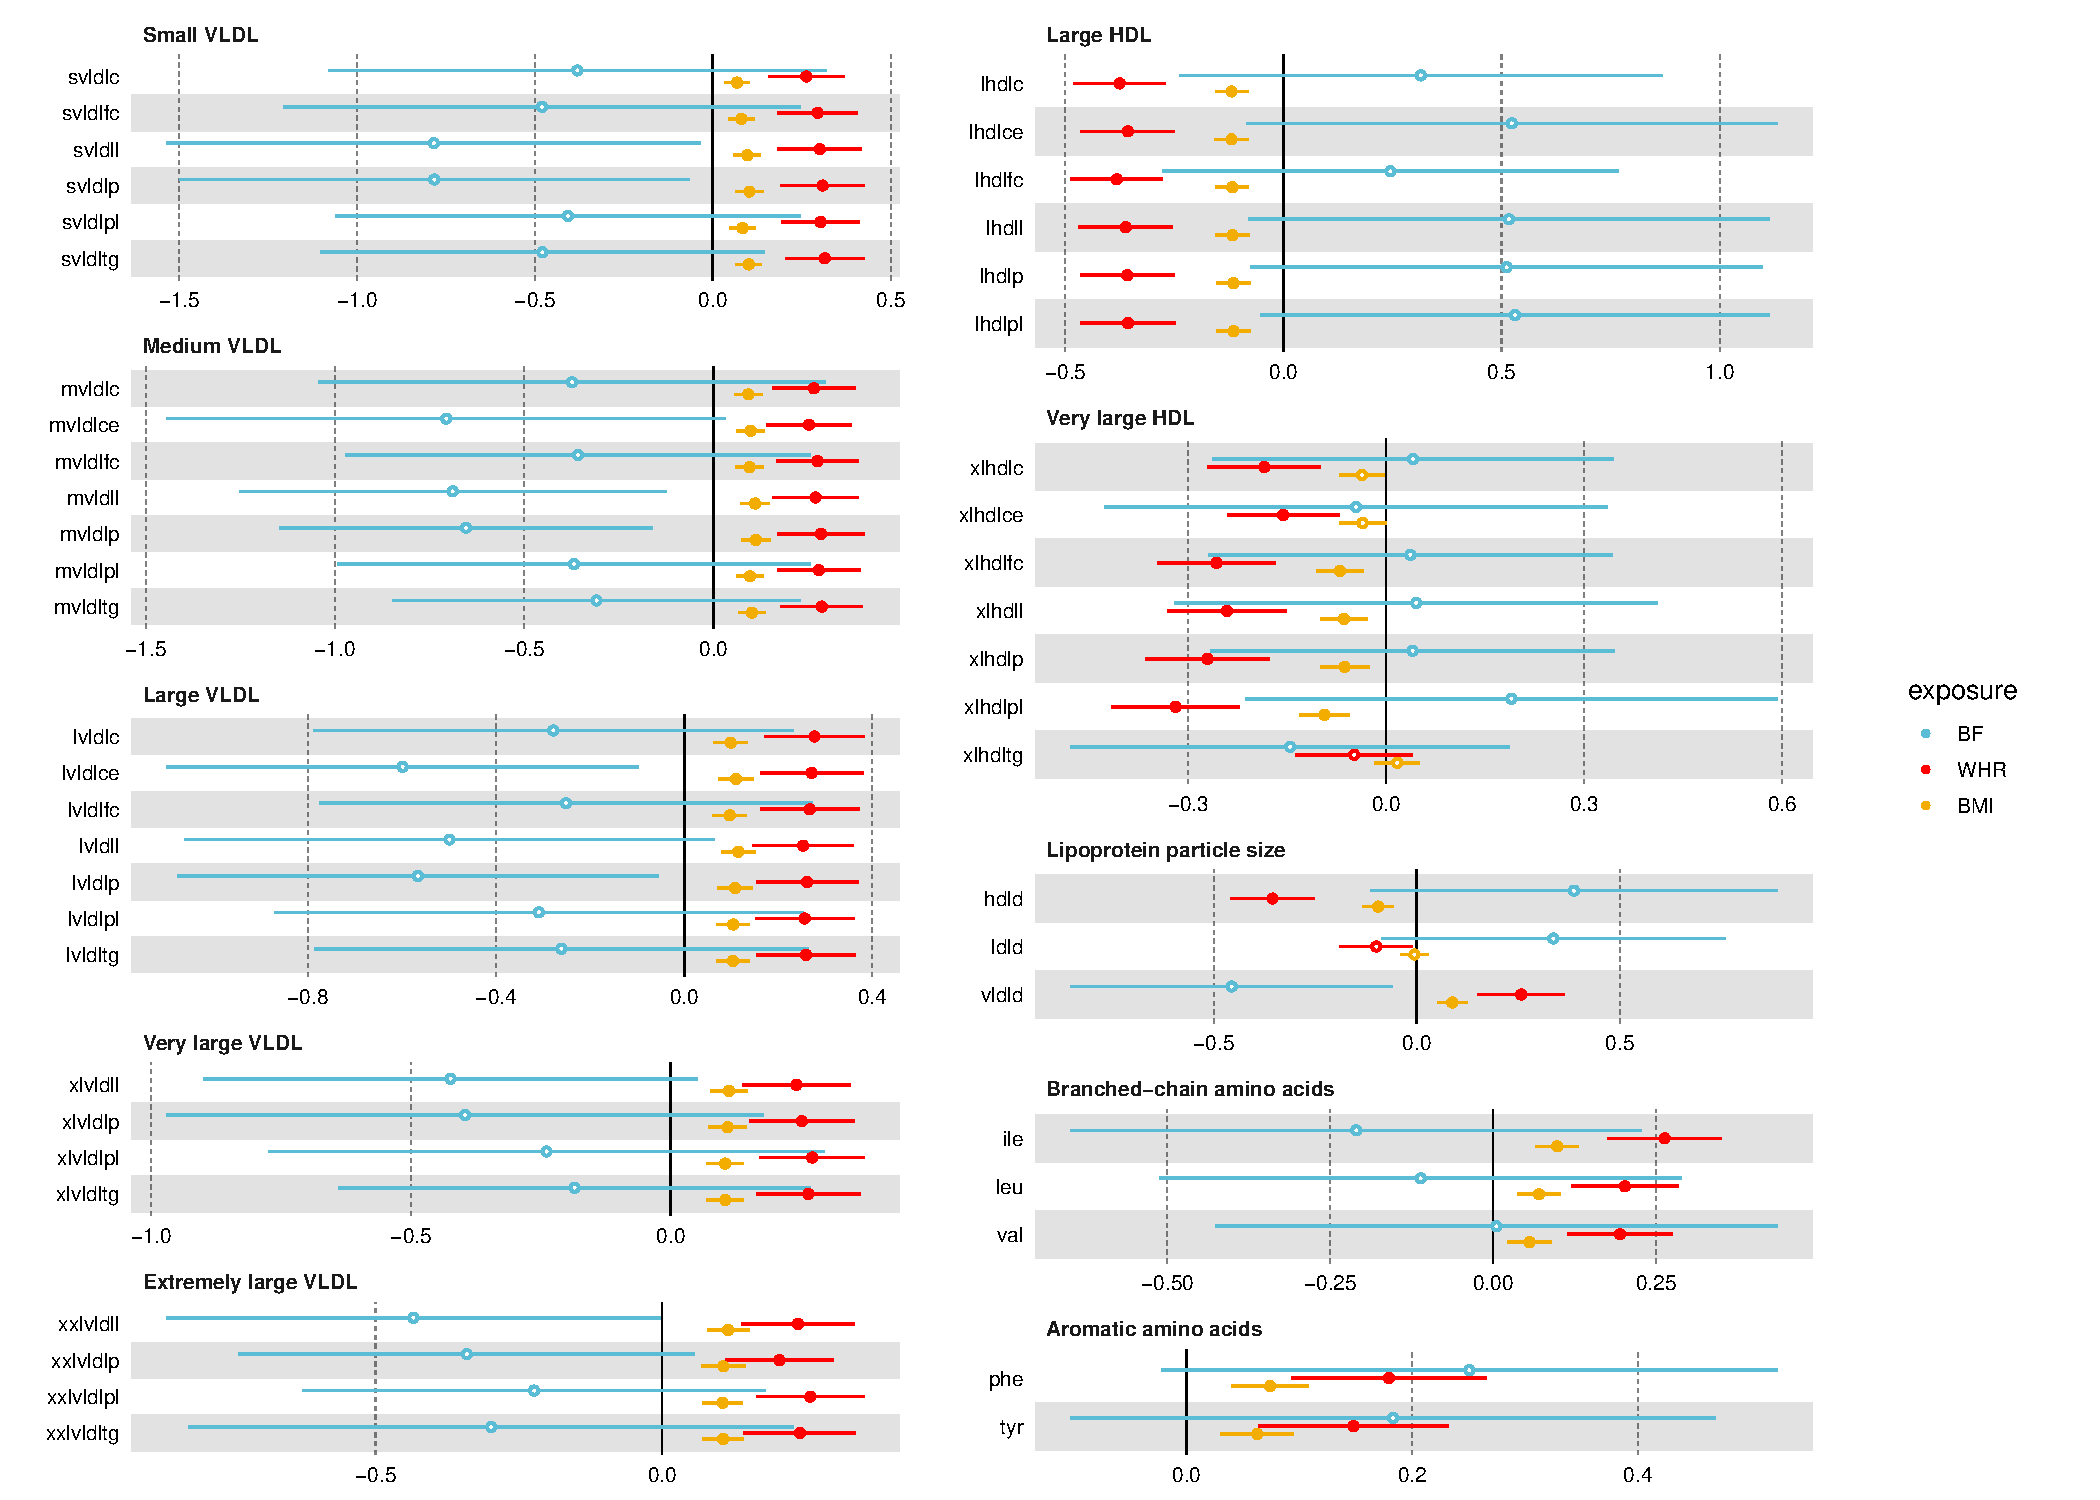
\includegraphics[width=1\linewidth]{data/chapter5/figures/forestplot_subclasses} \caption{Forestplot of effect estimates across subclasses with a majority of metabolites reaching a multiple testing threshold for BMI and WHR}\label{fig:chapter5-figure-forestplot-subclasses}
\end{figure}
\noindent 
\bsmall
\emph{Figure \ref{fig:chapter5-figure-forestplot-subclasses} gives effect estimates and 95\% confidence interval for all sublcasses in which the majority of metabolites reached a multiple testing threshold across BMI and WHR. Solid points reflect the multiple testing threshold (p \textless{} 0.05/22) has been reached.}
\esmall

\hypertarget{sensitivity-analysis-1}{%
\paragraph{Sensitivity analysis}\label{sensitivity-analysis-1}}

The majority of effect estimates for each metabolite showed directional consistency across the main analysis (IVW-MRE) and three models (MR-Egger, weighted median, weighted mode) used for sensitivity analysis for BMI (N = 69) and WHR (N = 98); BF showed the lowest directional concordance between models (N = 48; Figure \ref{fig:chapter5-figure-sensitivity-directional-consistency}). Of these directionally consistent tests within exposures and across methods, a total of 29 were directionally consistent across methods for all three exposures (Figure \ref{fig:chapter5-figure-forestplot-sensitivity-exposure} - direction of effect for BF was on the whole opposite to BMI and WHR for all methods. Of these 29, only \emph{Valine} was also found to be directionally consistent and reached a multiple testing threshold for both BMI and WHR in the main analysis (Figure \ref{fig:chapter5-figure-forestplot-associations}. Globally, sensitivity analysis was visually reflective of the main analysis for each exposure, though with wider confidnece intervals (Supplementary Figures \ref{fig:appendix-chapter5-figure-circosplot-sensitivity-main-BMI}, \ref{fig:appendix-chapter5-figure-circosplot-sensitivity-main-WHR}, \ref{fig:appendix-chapter5-figure-circosplot-sensitivity-main-BF}). Confidence intervals for sensitivity analyses tended to cross the null and were widest for MR Egger. Sensitivity results for WHR appeared to show most consistency with the main analysis; confidence intervals for weighted median and mode models did not cross the null in a majority of results for subclasses: \emph{Very Small VLDL}, \emph{Small VLDL}, \emph{Medium VLDL}, \emph{Large VLDL}, \emph{Very large VLDL}, \emph{Extremely large VLDL}, \emph{IDL}, \emph{Small LDL}, \emph{Medium LDL}, \emph{Large LDL}, \emph{Small HDL}, \emph{Medium HDL}, \emph{Large HDL}, \emph{Very large HDL} (Supplemetary FIgure \ref{fig:appendix-chapter5-figure-circosplot-sensitivity-main-WHR}).
\begin{figure}
\includegraphics[width=1\linewidth]{thesis_files/figure-latex/chapter5-figure-sensitivity-directional-consistency-1} \caption{Directional consistency across MR models for each exposure}\label{fig:chapter5-figure-sensitivity-directional-consistency}
\end{figure}
\noindent 
\bsmall
\emph{Directional consistency of all exposures from the main analysis: BMI (Yengo et al. (2018)), WHR (Pulit et al. (2018)), BF (Lu et al. (2016)). A positive effect reflects the effect estimate from two or more exposures being in the positive direction; a negative effect reflects betas being in a negative direction; opposite effect reflects different directions for the effect estimates. BMI = body mass index; WHR = waist hip ratio; BF = body fat percentage.}
\esmall
\begin{figure}
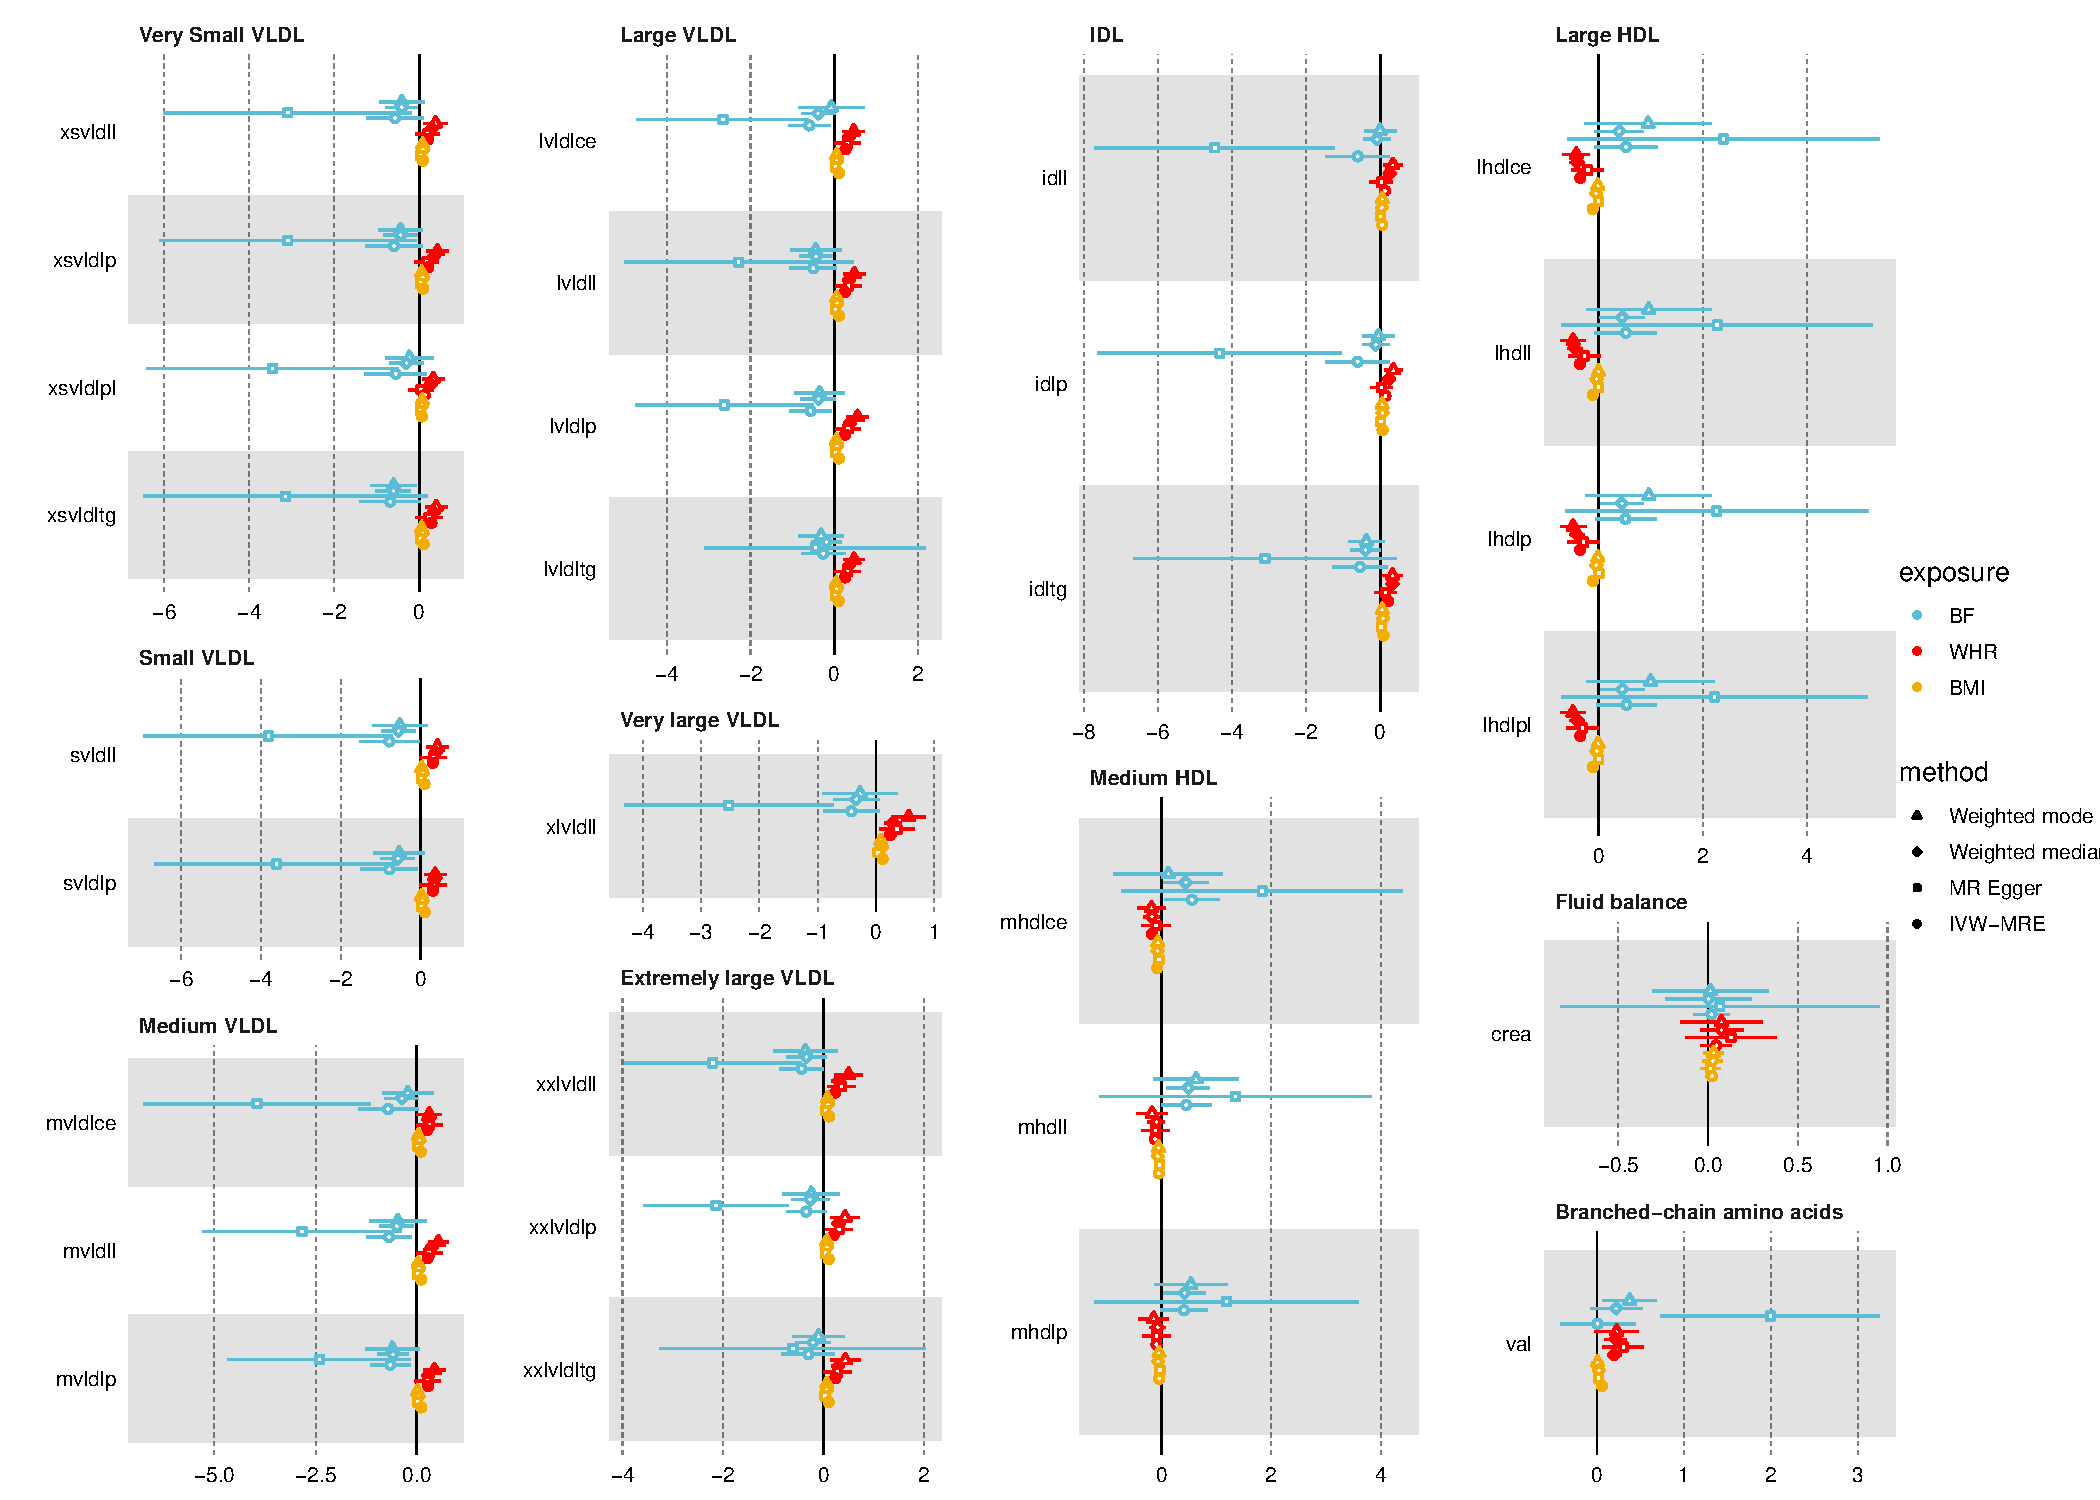
\includegraphics[width=1\linewidth]{data/chapter5/figures/forestplot_sensitivity_directional_consistency} \caption{Forestplot of directionally consistent results across methods within exposures}\label{fig:chapter5-figure-forestplot-sensitivity-exposure}
\end{figure}
\noindent 
\bsmall
\emph{Effect estimates and 95\% confidence intervals for metabolites which showed diectionally consistent results across the main (IVW-MRE = inverse variance weighted multiplicative random effects) and sensitivity analysis (MR-Egger, weighted median, weighted mode) within each exposure. Of the directionally consistent results within exposures, a total of 29 were identified within all three exposures and are presented here. BMI = body mass idnex (Yengo et al. (2018)); WHR = waist hip ratio (Pulit et al. (2018)); BF = body fat percentage (Lu et al. (2016)).}
\esmall

Heterogeniety of the genetic instruments for each exposure, measured using Cochrane's Q statistic, was greater than the degrees of freedom for a majority of metabolites for all three exposures (Table \ref{tab:chapter5-table-heterogeneity-N}).
\begin{table}

\caption{\label{tab:chapter5-table-heterogeneity-N}Number of tests in which Cochrane`s Q exceeds genetic instrumental variable degrees of freedom}
\centering
\begin{tabular}[t]{lrrr}
\toprule
 & ML & IVW & MR Egger\\
\midrule
BMI & 120 & 120 & 120\\
WHR & 121 & 121 & 121\\
BF & 112 & 111 & 112\\
\bottomrule
\end{tabular}
\end{table}
\noindent 
\bsmall
\emph{The number of tests (exposure on metabolite) for which Cochrane's Q statistic exceeded the degrees of freedom (number of SNPs - 1) for each exposure. ML = maximum likelihood method, IVW = Inverse variance weighte dmethod; BMI = body mass idnex, WHR = waist hip ratio, BF = body fat percentage.}
\esmall

In single SNP MR analysis, visual inspection of forest plots showed characteristcly \(S\) shaped distributions of effect estimates for all tests (Representative Figure \ref{fig:appendix-chapter5-figure-singlesnp-representative-figure}; all figures GitHub). Funnel plots for BMI and WHR highlighted a number of SNPs lying outside of the funnel distribution which were investigated further (Representative Figure \ref{fig:appendix-chapter5-figure-funnelplot-BMI-representative-figure} - the low number of SNPs used for BF did not result in meaningfully interpretable funnel plots (Representative Figure \ref{fig:appendix-chapter5-figure-funnelplot-BMI-representative-figure}. Effect estimates for some SNPs in the single SNP MR analysis appeared to be outliers, for example for BMI, rs4673553 showed a disproprotinately larger effect estimate of 22 (standard error = 0.85; \emph{p-value} = 5.66 x 10\textsuperscript{-148}) for Glycoproteins when compared to other SNPs. Additionally, rs7777102 showed a disproprotinately larger effect estimate of -9 for Mean diameter for VLDL particles (standard error = 1.14; \emph{p-value} = 6.15 x 10\textsuperscript{-17}). Looking at the median effect size across all metabolites for each SNP, a number of SNPs (including rs7777102 for BMI) showed dispraportionately larger median effect sizes. The number of SNPs with median effect estimates at the extremes (5\% and 95\%) were: BMI = 46 (5\%) and 46 (95\%); WHR = 46 (5\%) and 46 (95\%); BF = 1 (5\%) and 1 (95\%).

In leave-one-out analysis, visual inspection of forest plots showed that no single SNP altered the direction of effect for any metabolite across exposures. For BF, confidence intervals for one or more SNPs crossed the null for every metabolite tested (Representative Figure \ref{fig:appendix-chapter5-figure-leaveoneout-BF-representative-figure}; all figures GitHub). This was not the case for BMI and WHR, where for many metabolites confidence intervals did not cross the null for any SNPs (Representative Figure \ref{fig:appendix-chapter5-figure-leaveoneout-BMI-representative-figure}; all figures GitHub).

\hypertarget{additional-analyses-1}{%
\subsection{Additional analyses}\label{additional-analyses-1}}

\hypertarget{additional-exposures}{%
\subsubsection{Additional exposures}\label{additional-exposures}}

Results from additional exposures for BMI showed broadly larger effect estimates but consistent directions of effect across metabolites (Figure \ref{fig:chapter5-figure-circosplot-additional-BMI}). For the BMI SNPs obtained from a non-UK Biobank GWAS, effect estimates had much wider confidence intervals. Spearman's Rho correlataion of MR results was highest between the two SNP lists from Yengo et al. (2018) (0.98) - correlation between the the Locke et al (2014) SNP list and the COJO SNP list from Yengo et al (2018) (0.9) and the non-COJO SNP list from Yengo et al. (2018) (0.93) were also high.
\begin{figure}
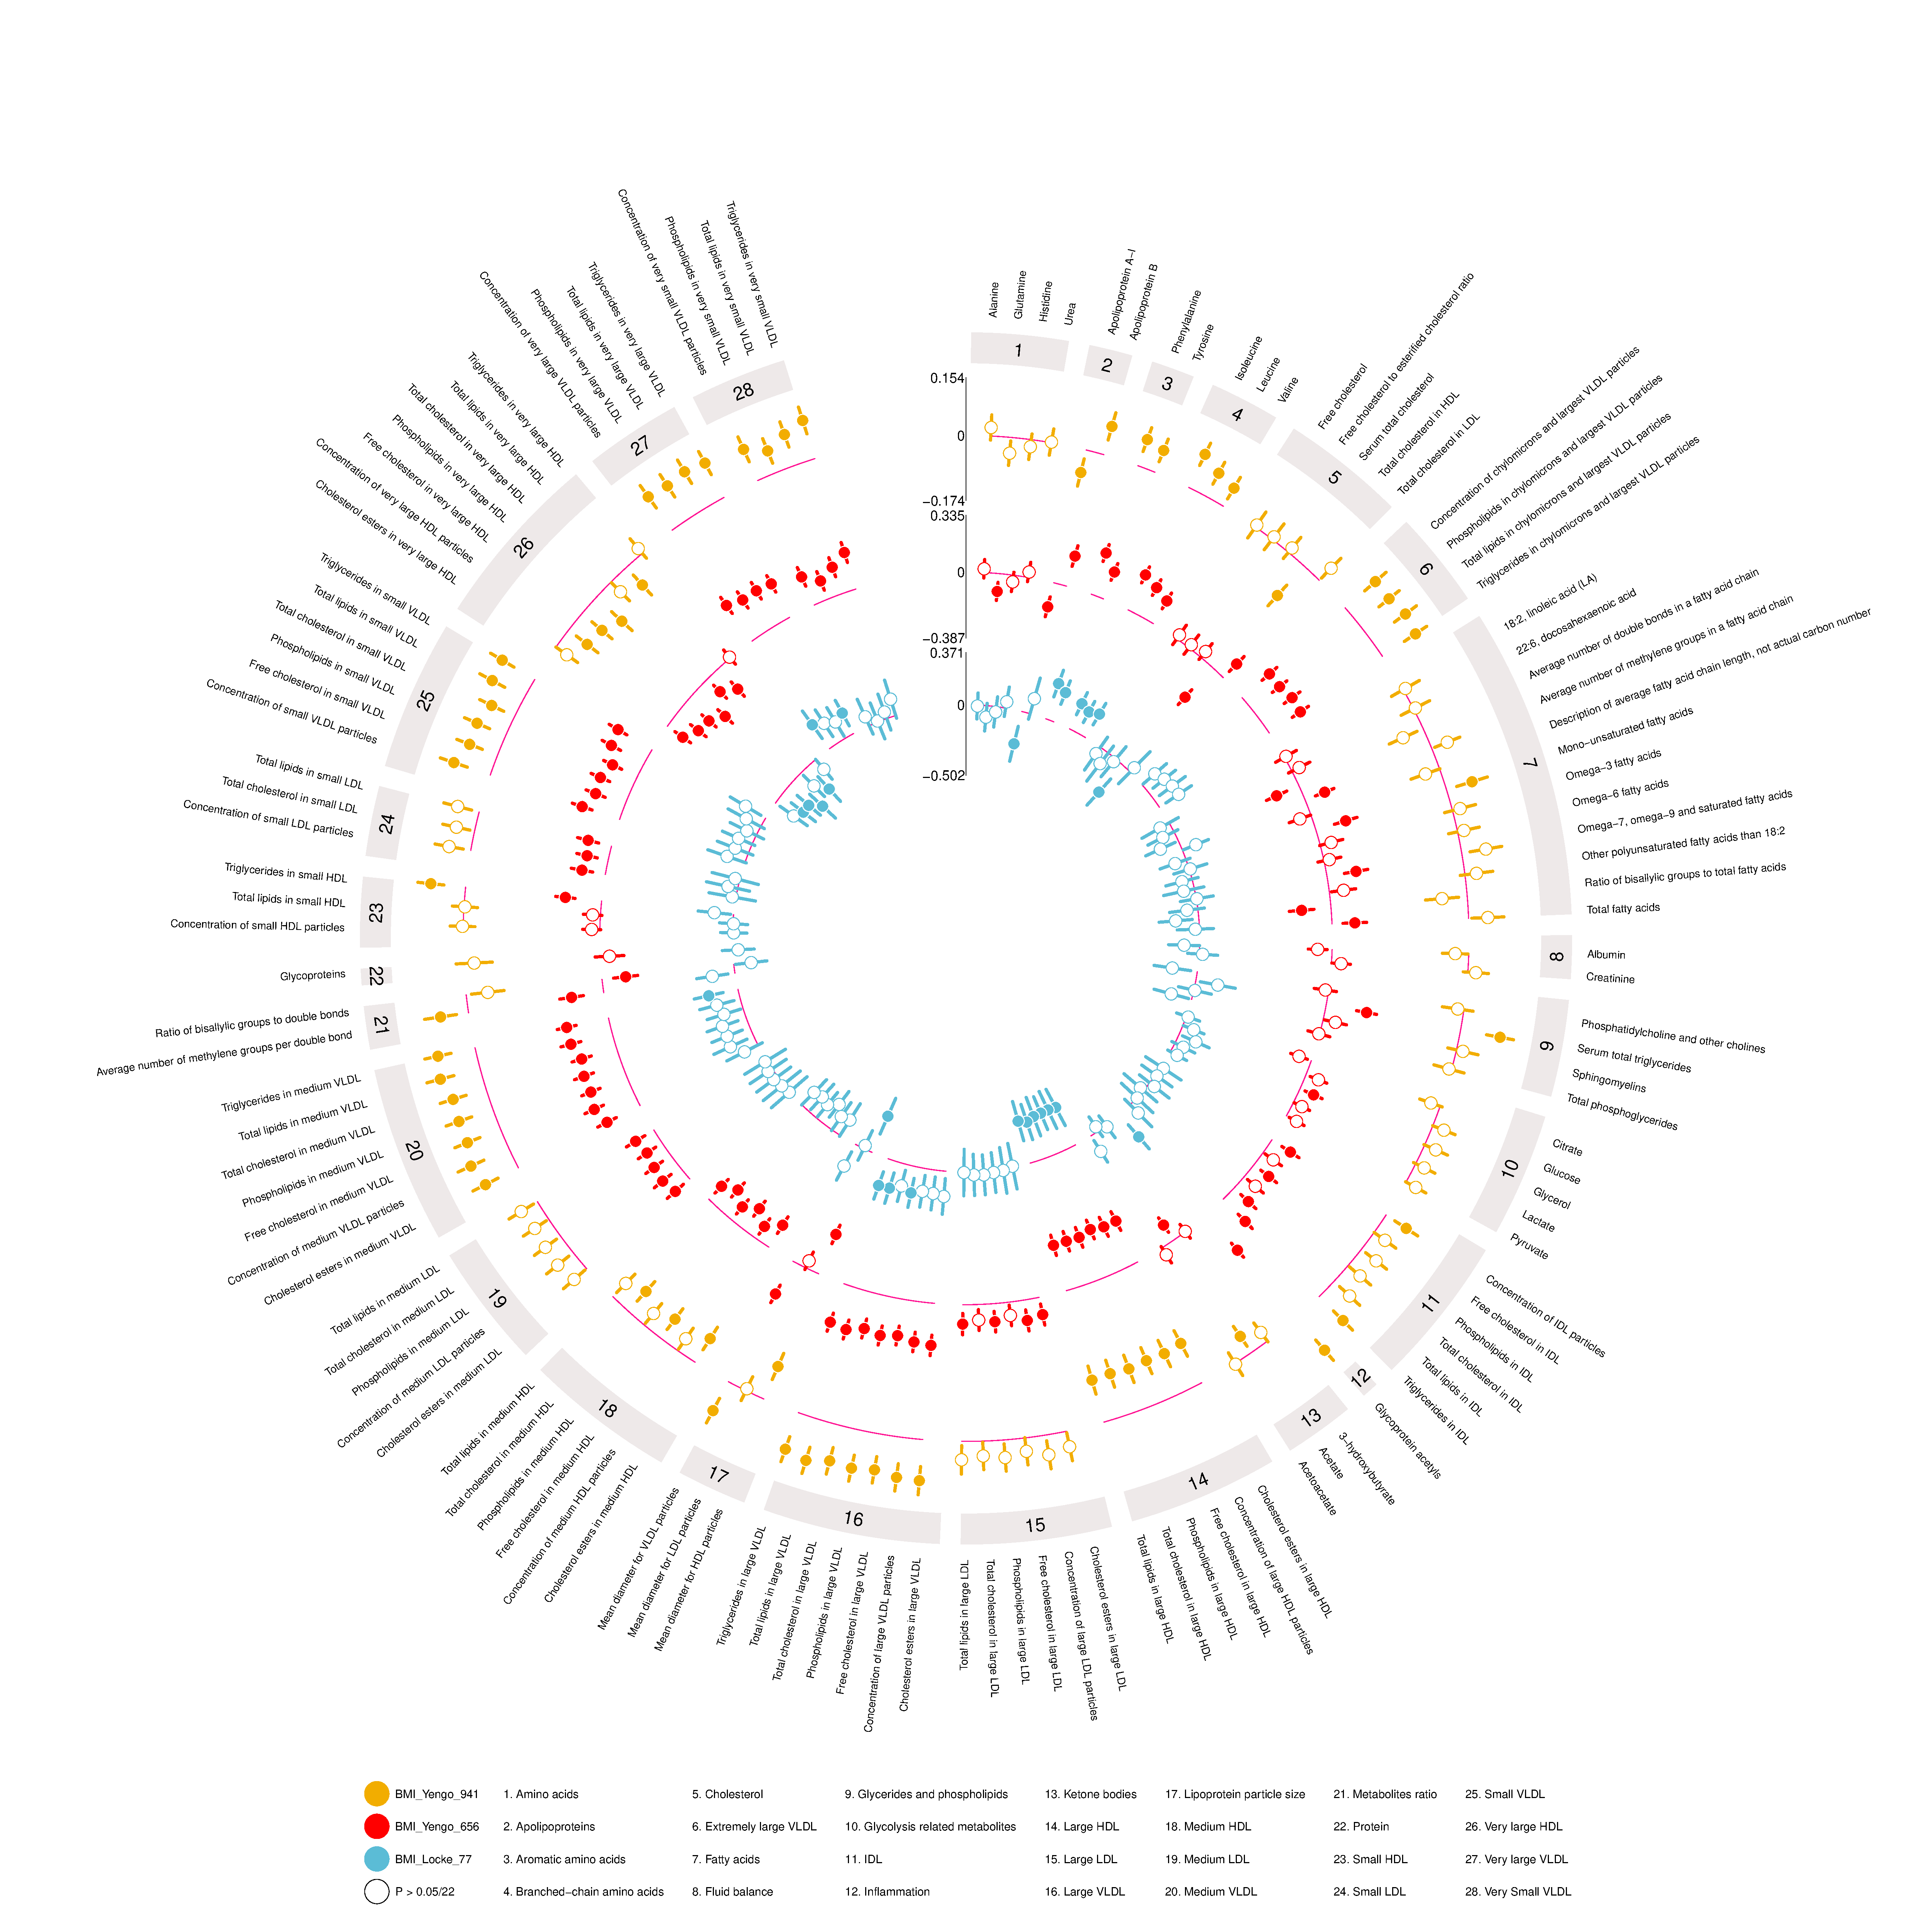
\includegraphics[width=1\linewidth]{data/chapter5/figures/circosplot_additional_BMI} \caption{Circos plot of IVW-MRE effect estimates for three different BMI SNP lists on 123 NRM derived metabolites}\label{fig:chapter5-figure-circosplot-additional-BMI}
\end{figure}
For WHR the global pattern of association was similar between both the main and additional exposure (Figure \ref{fig:chapter5-figure-circosplot-additional-BMI}) with high correlation between MR results (0.9). Effect estimates were larger for the additional exposure from Shungin et al (2014), for which fewer reuslts reached the multiple testing threshold with wider confidence intervals which crossed the null more often than with the main analysis.
\begin{figure}
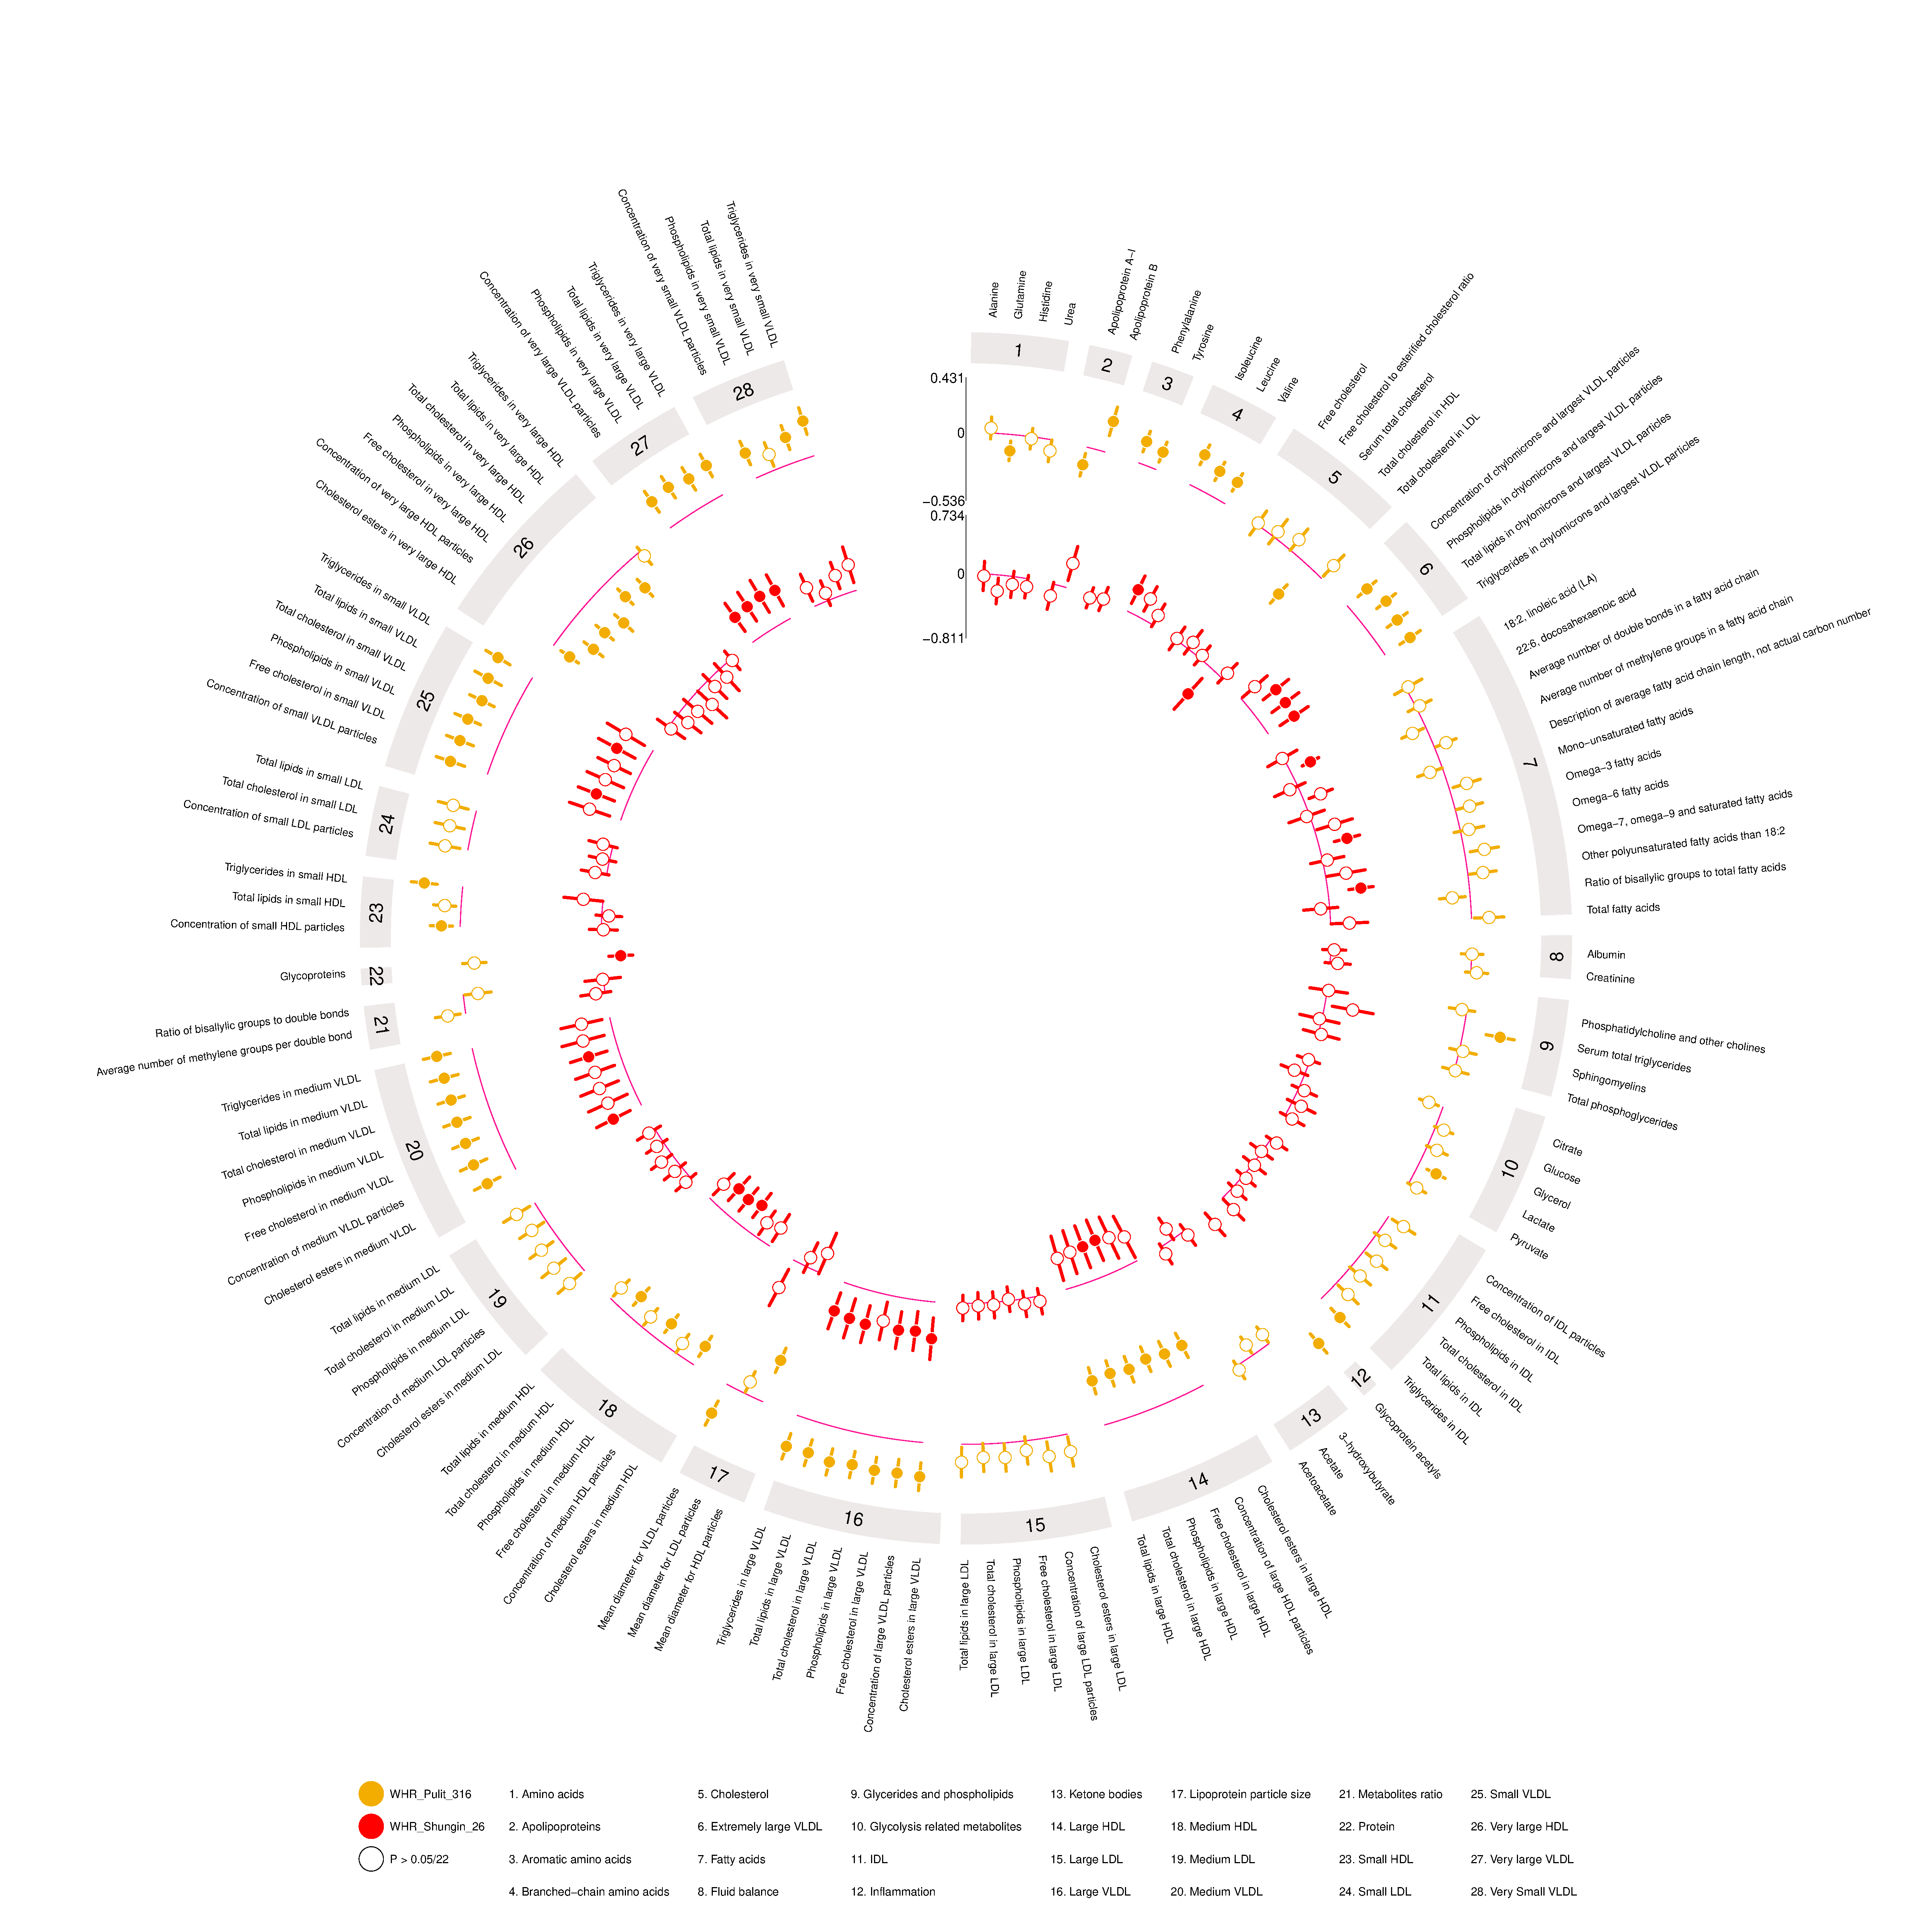
\includegraphics[width=1\linewidth]{data/chapter5/figures/circosplot_additional_WHR} \caption{Circos plot of IVW-MRE effect estimates for two different WHR SNP lists on 123 NRM derived metabolites}\label{fig:chapter5-figure-circosplot-additional-WHR}
\end{figure}
For BF there was considerable similarity between the main analysis and the additional analysis from Lu et al (2016) which did not include two SNPs previousy identified as being associated with favourable adiposity (Figure \ref{fig:chapter5-figure-circosplot-additional-BF}). More metabolites reached the multiple testing threshold when using the 5 SNPs from Lu et al (2016) as opposed to the full 7 SNPs, this included associations with Apolipoprotein A1, Phenylalanine, Tyrosine, Glucose, and Cholesterol esters in very large HDL. For the additional analysis which used 76 SNPs from Hubel et al (2016), MR reuslts were considerbaly smaller and appeared to show conflicting directions of effect with that of the Lu et al. (2016) SNPs (both using 7 and 5 SNPs). Confidence intervals were much tighter and two metabolites (Phenylalanine and Glycoprotein acetyls) reached the multiple testing threshold. Correlation between the two Lu et al (2016) SNP lists was high (0.93), however both the 5 (-0.64) and 7 (-0.52) SNP lists from Lu et al. (2016) showed weaker inverse correaltions with the SNP list from Hubel et al (2016).
\begin{figure}
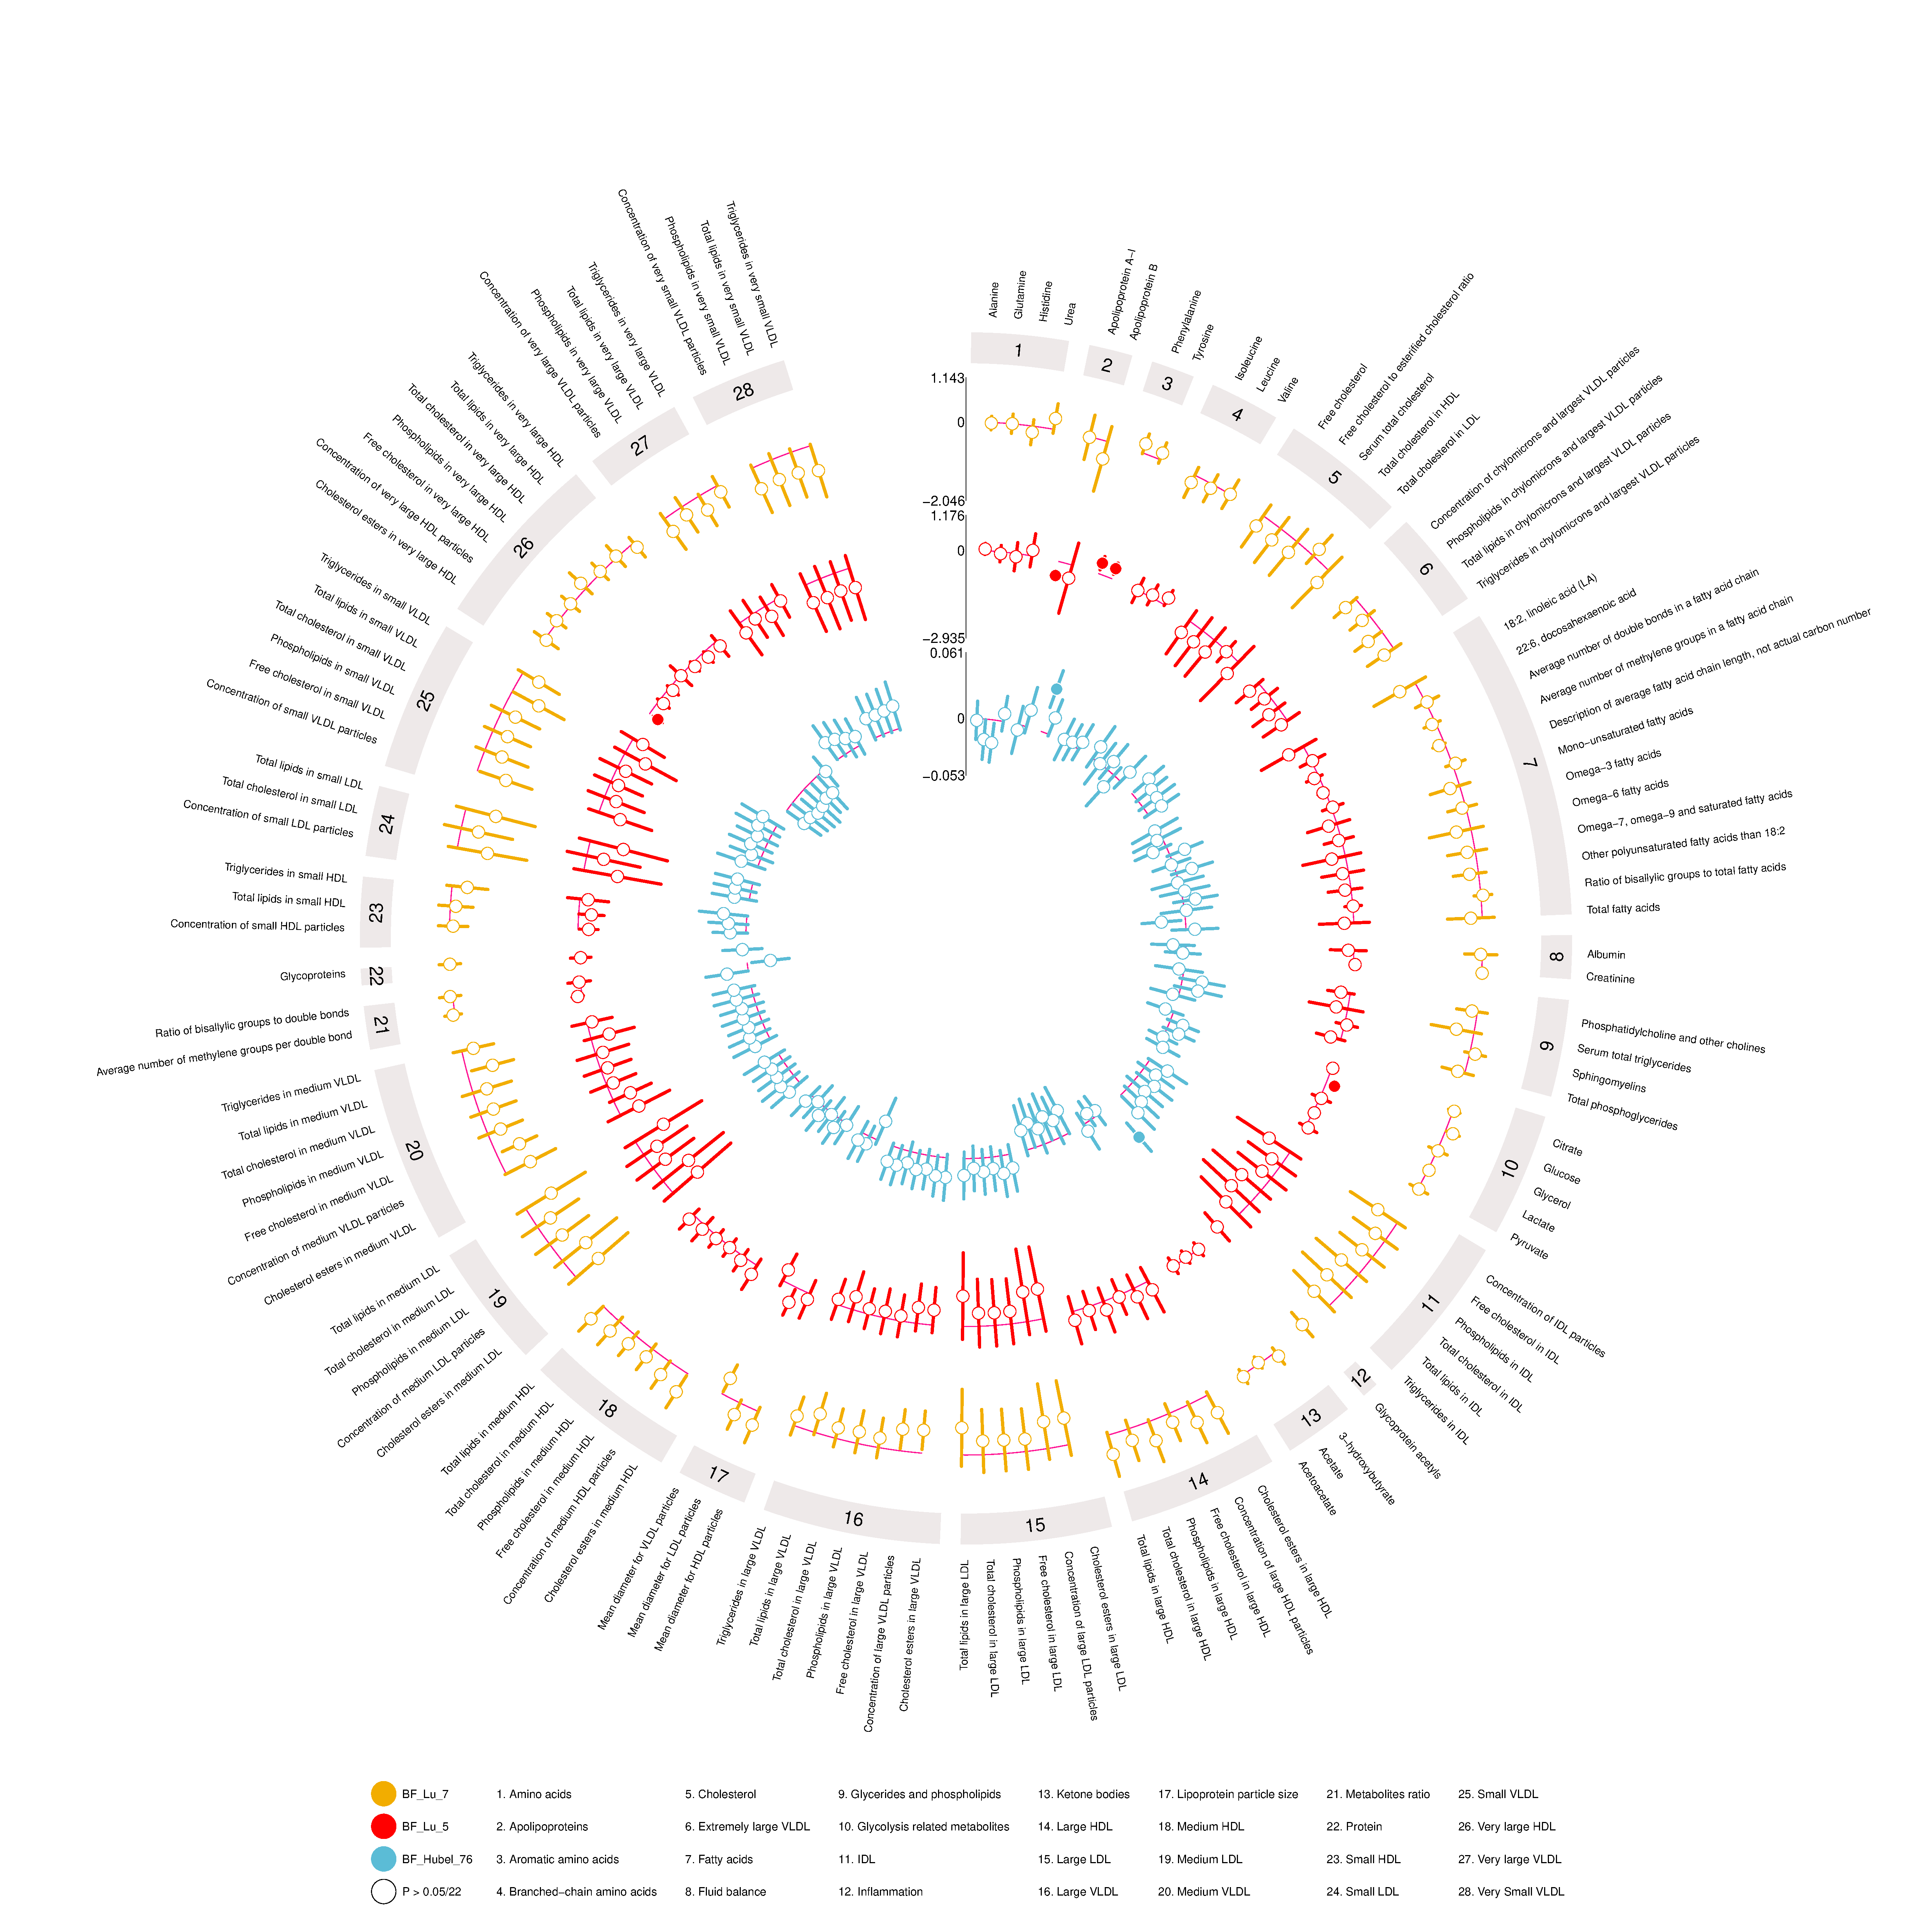
\includegraphics[width=1\linewidth]{data/chapter5/figures/circosplot_additional_BF} \caption{Circos plot of IVW-MRE effect estimates for three different BF SNP lists on 123 NRM derived metabolites}\label{fig:chapter5-figure-circosplot-additional-BF}
\end{figure}
\hypertarget{clumped-exposures}{%
\subsubsection{Clumped exposures}\label{clumped-exposures}}

All SNP lists used as exposures underwent clumping and MR analyses were repeated. Clumping resulted in the removal of the following SNPs due to LD (R\textsuperscript{2} \textgreater{}= 0.001) with other variants or absence from the LD reference panel: BMI Locke et al. (2014) = 14, BMI Yengo et al. (2018) using COJO SNPs = 583, BMI Yengo et al. (2018) using non-COJO SNPs = 336, WHR Pulit et al. (2018) = 234, WHR Shungin et al. (2014) = 17, BF Hubel et al. (2018) = 4. No SNPs were removed due to clumping for BF from Lu et al. (2016)\textsuperscript{\protect\hyperlink{ref-Lu2016}{183}}. All SNPs, including whether they were removed due to clumping, are presented in the Supplement (Table \ref{tab:appendix-chapter5-table-exposures}).

For BMI, correlation between the Yengo COJO (0.9731849), non-COJO (0.9670003), and Locke (0.9782216) non-clumped and clumped MR results was high. Similarly, for WHR MR results from non-clumped and clumped analyses correlation was high for the main exposure (Pulit et al. (2018) = 0.974436) and for the additional exposure (0.9766674). For BF, clumping was not possible for the main exposure, however correlation between the non-clumped and clumped SNP list from Hubel et al. (2018) was high (0.9808851).

\hypertarget{comparison-with-observational-estimates-from-chapter-refchapter4}{%
\subsection{Comparison with observational estimates from Chapter \ref{chapter4}}\label{comparison-with-observational-estimates-from-chapter-refchapter4}}

In total, 111 metabolites were measured across the observational analysis in adults (conducted in Chapter \ref{chapter4}) and the main MR analysis conducted here. Of these, a majority of metabolites showed consistent directions of effect when comparing within exposures between MR and observational results for BMI (n = 107; Spearmans correlation between MR and observational results = 0.56) and WHR (n = 108; Spearmans correlation between MR and observational results = 0.55;Figure \ref{fig:chapter5-figure-directional-consistency-comparison}). For BF, a majority (n = 93; Spearmans correaltion between MR and observational results = -0.69) of metabolite results showed opposite directions of effect, e.g.~a positive direction of effect may be observed for an MR result but a negative direction of effect for the same metabolite may be observed for the observational analysis.
\begin{figure}
\includegraphics[width=1\linewidth]{thesis_files/figure-latex/chapter5-figure-directional-consistency-comparison-1} \caption{Directional consistency across exposures}\label{fig:chapter5-figure-directional-consistency-comparison}
\end{figure}
\noindent 
\bsmall
\emph{Figure \ref{fig:chapter5-figure-directional-consistency-comparison} shows the directional consistency between the MR and aboservational analyses for BMI, WHR, and BF exposures. A positive effect reflects the effect estimate from two exposures being in the positive direction; a negative effect reflects betas being in a negative direction; opposite effect reflects different directions for the effect estimates. BMI = body mass index; WHR = waist hip ratio; BF = body fat percentage.}
\esmall

Across the 111 metabolites, a total of 62 reached the multiple testing threshold for BMI in both observational (observational only = 101) and MR (MR only = 62) analyses. This was similar for WHR, where 63 metabolites reached a multiple testing threshold across both observational (observational only = 102) and MR (MR only = 63) analyses. For BF there were 0 metabolites that reached the multiple testing threshold across both MR and observational analyses. This was a result of 0 metabolites reaching the multiple testing threshold in the MR analysis - for the observational analysis a simialr number of metabolites reached the multiple testing threshold (100) as with the BMI and WHR observational analyses.

Of the 62 metabolites that reached the multiple testing threshold for BMI, a total of 62 were directionally consistent across both MR and observational analyses; 45 tests showed a positive direction of effect and 17 showed a negative direction of effect. For WHR, of the 63 metabolites reaching the multiple testing threshold across MR and observational analyses, a total of 63 metabolites were directionally consistent; 45 showed a positive direction of effect and 64 showed a negative direction of effect. When looking at both MR and observational results across BMI and WHR there are a total of 67 metabolites which reach a multiple testing threshold, of these 4 are unique to BMI and 5 are unique to WHR. Combined, there were 58 metabolites which reached the multiple testing threshold across BMI and WHR for MR and observational analsyes. Of these 58, a total of 58 metabolites were directionally consistent across BMI and WHR; 42 showed a positive direction of effect and 16 showed a negative direction of effect.

Across observational and MR analyses for BMI and WHR, 58 results were directionally consistent and met a multiple testing threshold. When looking at these metabolites across all three exposures for MR and observational analyses (Figure \ref{fig:chapter5-figure-forestplot-directional-consistency-comparison}): MR results have wider confidence intervals than observational results, WHR in MR analysis shows broadly larger effects across a majority of metabolites, effect size for BMI in MR analysis is broadly consistent with the three exposures in observational analyses, confidence intervals for BF in MR analysis spans most of the effect estimates for the MR and observational results across a majority of metabolites.
\begin{figure}
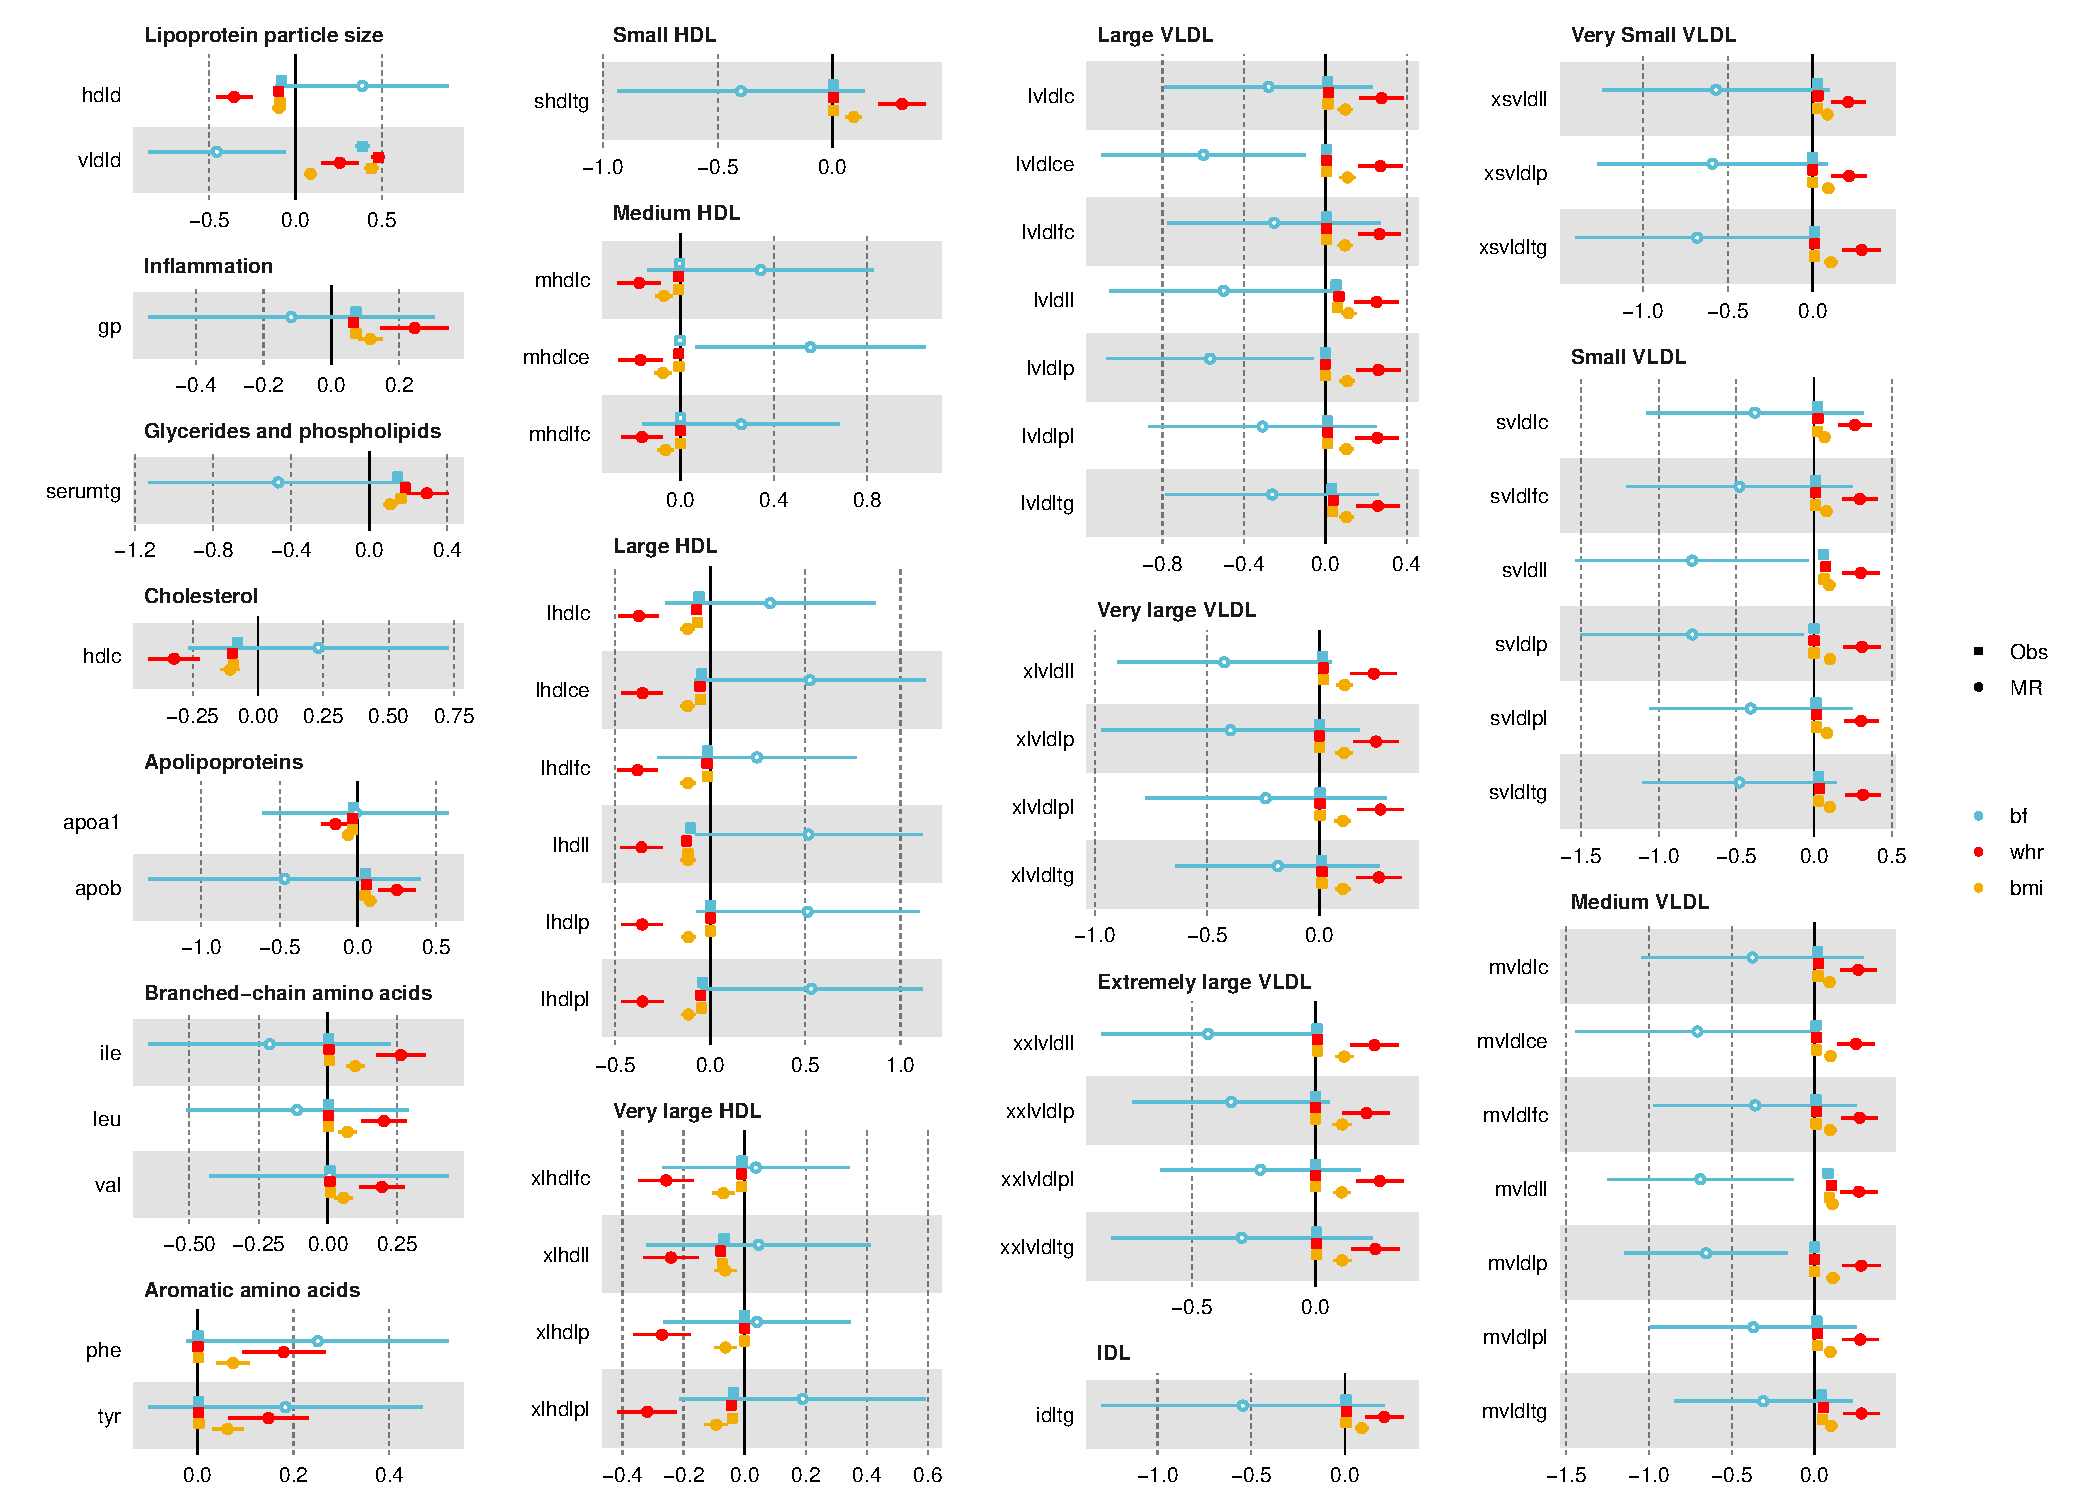
\includegraphics[width=1\linewidth]{data/chapter5/figures/forestplot_sensitivity_directional_consistency_comparison} \caption{Directional consistency across exposures}\label{fig:chapter5-figure-forestplot-directional-consistency-comparison}
\end{figure}
\noindent 
\bsmall
\emph{Figure \ref{fig:chapter5-figure-forestplot-directional-consistency-comparison} shows the directional consistency between the MR and aboservational analyses for BMI, WHR, and BF exposures. A positive effect reflects the effect estimate from two exposures being in the positive direction; a negative effect reflects betas being in a negative direction; opposite effect reflects different directions for the effect estimates. BMI = body mass index; WHR = waist hip ratio; BF = body fat percentage.}
\esmall

\hypertarget{comparison-with-wurtz-et-al.-2014wurtz2014-1}{%
\subsubsection{\texorpdfstring{Comparison with Wurtz et al. (2014)\textsuperscript{\protect\hyperlink{ref-Wurtz2014}{149}}}{Comparison with Wurtz et al. (2014)149}}\label{comparison-with-wurtz-et-al.-2014wurtz2014-1}}

Of the 58 metabolites that were directionally consistent across BMI and WHR and met a multiple testing threshold, for both MR and observational analyses, 11 were also analysed previously by Wurtz et al. (2014)\textsuperscript{\protect\hyperlink{ref-Wurtz2014}{149}}. Comparison of effect estimates across all exposures from MR and observational analysis with results from Wurtz et al. (2014) is presented in Figure \ref{fig:chapter5-figure-forestplot-directional-consistency-comparison-wurtz}. Observational results (described in \ref{chapter4-wurtz-comparison}) were comparable with observational results from Wurtz et al. (2014) in their direction of effect, and broadly comparable in effect size with overlapping confidence intervals. For the 11 results here however the \emph{Amino acids} subclasses metabolites showed large differences in effect size in both observational and MR analysis compared with Wurtz et al. (2014). Effect sizes were much more similar for the metabolites in the remaining subcalsses (\emph{Lipoprotein particle size}, \emph{Inflammation}, \emph{Cholesterol} and \emph{Apolipoproteins}), however MR results from analysis conducted here was broadly larger.
\begin{figure}
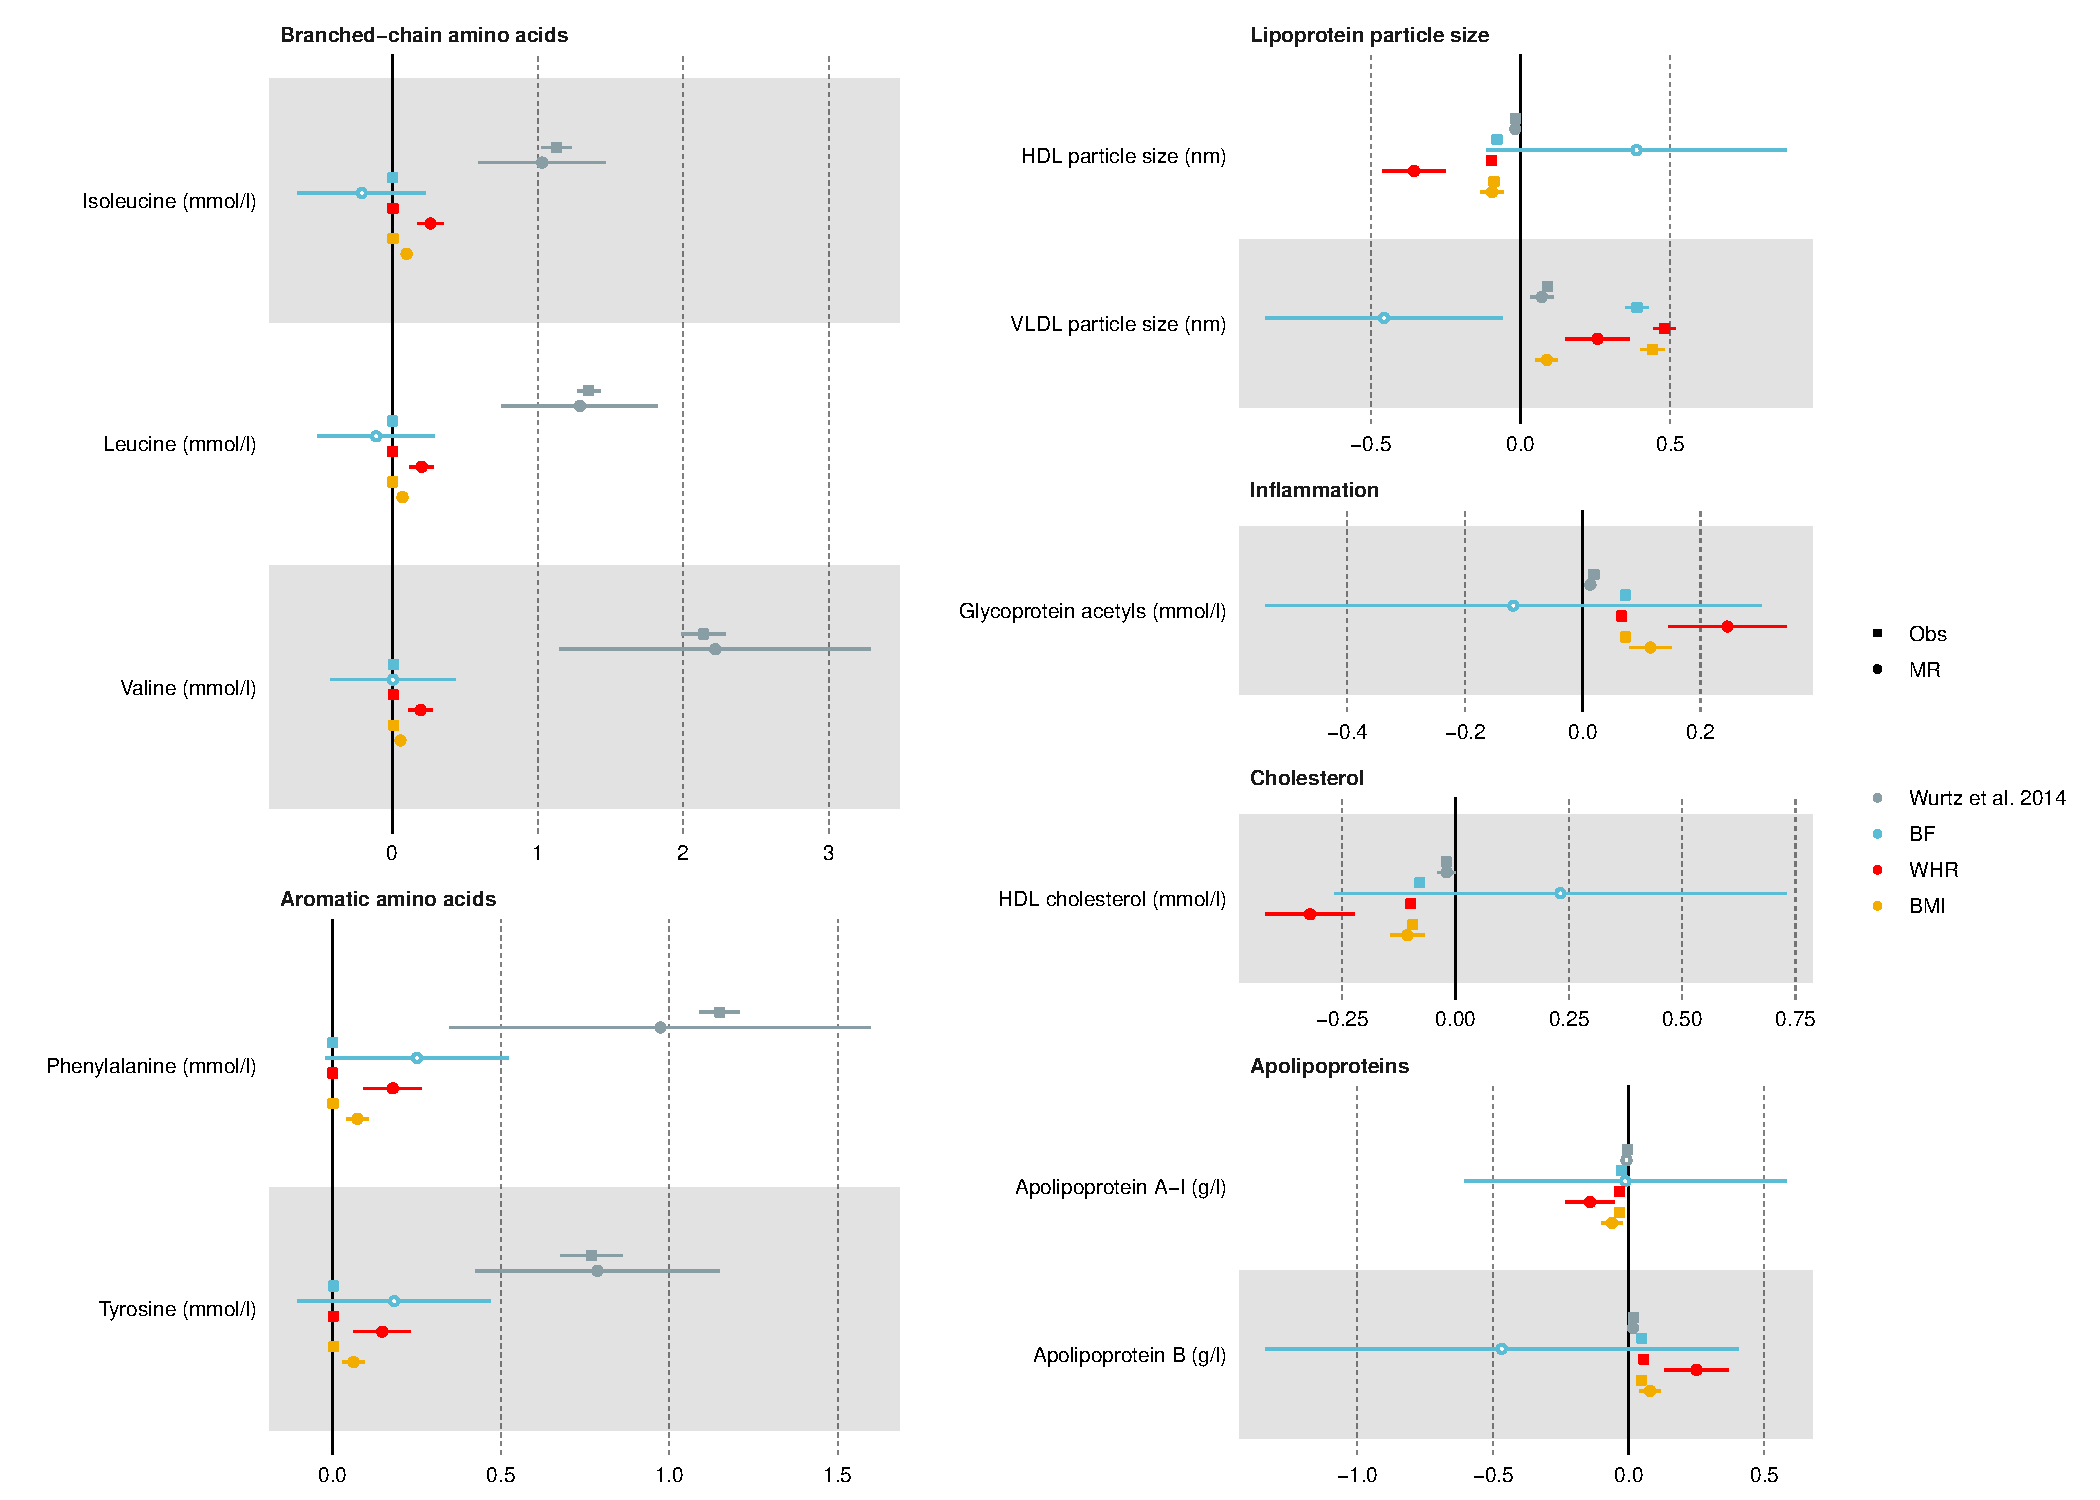
\includegraphics[width=1\linewidth]{data/chapter5/figures/forestplot_sensitivity_directional_consistency_comparison_wurtz} \caption{Comparison of MR and observational results with observational and MR results from Wurtz et al. (2014)}\label{fig:chapter5-figure-forestplot-directional-consistency-comparison-wurtz}
\end{figure}
\hypertarget{discussion}{%
\section{Discussion}\label{discussion}}

In this chapter, the influence of increased adiposity on the metabolic profile is demonstrated in an MR framework. The use of MR allowed for the interrogation of causality between BMI, WHR, and BF with the metabolic profile, while accounting for limitations in observational analyses (discussed in Chapter \ref{chapter1} and \ref{chapter4}).

Results for BMI and WHR provide evidence for a global association; both show positive and negative effects on whole subclasses of metabolites. On the whole, WHR showed a larger effect across the metabolic profile, however confidence intervals for WHR and BMI mostly overlapped with one another. Evidence for an association between BF and the metabolic profile was lacking; on the whole, directions of effect conflicted with those of BMI and WHR, while effect estimates were larger and confidence intervals much wider.

Sensitivity analysis was broadly consistent with the main analysis across BMI and WHR; \emph{Valine} was the only metabolite that was directionally consistent in sensitivity analysis across BMI and WHR and which reached a multiple testing threshold in the main analysis. There was considerable heterogeneity in the genetic instruments used in the main analysis and in single SNP MR analysis a number of SNPs showed disproportionately larger effect estimates across many metabolites; leave-one-out analysis did not highlight any individual SNP as driving the effect for any metabolite.

Additional analysis aimed to assess whether instruments for BMI and WHR were appropriate given present structural problems in UK Biobank\textsuperscript{\protect\hyperlink{ref-Haworth2019}{89}} for which instruments were obtained, and whether BF instruments obtained from a GWAS using a mixture of measurment techniques were appropriate. In addition, though studies often report SNPs as being \emph{independent}, whether they are in an MR context was tested by clumping all instrument lists and repeating analyses. Use of additional BMI and WHR exposures showed consistent results with the main analysis, though the widening of confidence intervals obsevred for the non-UK Biobank SNP lists would suggest a considerable increase in power is present when using the larger SNP lists. Considerable difference was observed for BF, where the additional SNP list obtained from UK Biobank resulted in very small effect estimates which on the whole were inverse to the main BF analysis; removal of 2 SNPs from the main BF SNP list resulted in tighter confidence intervals and a number of metabolites reaching the multiple testing threshold -- these metabolites showed evidence of association for BMI and WHR in the main analysis. Clumping of SNP lists resulted in large numbers of SNPs being removed from the main BMI and WHR analyses, however results from all clumped and non-clumped SNP lists were highly correlated.

Taken together, results from the main, sensitivity, and additional analyses provide evidence for association between BMI and WHR and metabolites across a majority of subclassed. Though the main analysis for BF showed inconclusive evidence for association, additional analysis highlighted a number of metabolites that were found to be associated with BMI and WHR.

In Chapter \ref{chapter4} observational analysis of BMI, WHR, and BF highlighted association with the global metabolic profile that persisted across time and when adjusted for confounders. Of 111 metabolites measured across observational and MR analyses, all most all showed consistent directions of effect for BMI and WHR. Results for BF however, showed a majority of MR results to be in the opposite direction to observational results. Though correlation between MR and observational results was not very high, when taking into account directional consistency and the multiple testing threshold across MR and observational analysis between BMI and WHR just under half of the metabolites met this criteria. Previous work by Wurtz et al. (2014)\textsuperscript{\protect\hyperlink{ref-Wurtz2014}{149}}, discussed in relation to the observational analysis in Chapter \ref{chapter4}, highlighted causal associations between adolescent BMI and nuermous metabolites. In comparing results that met the above threshold with those of Wurtz et al. (2014) there is considerable difference in effect size across the board, this is particularly evident for metabolites in the \emph{Amino acids} subclasses.

\hypertarget{limitations}{%
\subsection{Limitations}\label{limitations}}

\hypertarget{metabolomics}{%
\subsubsection{Metabolomics}\label{metabolomics}}

As discussed in the limitations section of Chapter \ref{chapter4}, there is no standardised approach, nor a gold standard, for performing metabolomics quality control. In Chapter \ref{chapter4}, quality control, including outlier detection and removal, was performed using the \texttt{MetaboQC} \texttt{R} package. Metabolite data here however was obtained from previously reported GWAS's, in which studies used different collection and storage methods. Metabolomics analysis was consistent across all studies and adjustment prior to GWA analysis was made for age, sex, time from last meal if applicable, and the first ten genomic principal components. These adjustments were not all made in the observational analysis. In addition, no description of metabolomic data quality control prior to GWA analysis was provided and so compariosn with that applied in Chapter \ref{chapter4} is difficult.

\hypertarget{exposures}{%
\subsubsection{Exposures}\label{exposures}}

Given that MR relies on the use of an instrument to model the effect of an exposure on an outcome, that instrument needs to be robust and applicable to the exposure. The strength of an exposure is usually measured via an \(F\) statistic, for which an arbitrary threshold of \textgreater{} 10 denotes a strong instrument. All of the instruments used here exceeded this threshold. In addition, the variance explained in an exposure by a GWAS can indicate the power afforded in the MR analysis; the variance explained for exposures used in the main analysis varied from \textasciitilde{}22\% for WHR, to 6\% for BMI and \textasciitilde{}0.4\% for BF. The considerably lower variance explained for BF may have impacted on results, as when instruments which explained less variance for BMI and WHR were used confidence intervals became wider.

The consistent directions of effect observed across BMI and WHR measures adds weight to their associations with metabolites. For BF, conflicting directions of effect were observed when comparing to BMI and WHR. However, confidence intervals were wider and, although they spanned the null in all cases, included the estimates and confidence intervals for BMI and WHR in a majority of cases. There was considerable difference in the sample sizes used in the GWASs for BMI, WHR, and BF. In addition, whereas BMI and WHR were measured in only one way for their respective GWASs, the BF GWAS included measures of BF from DXA and impedance devices. Though, as shown in Chapter \ref{chapter4}, DXA and impedance measures of BF are highly correlated, the additional analysis for BF which used only impedance measures in the GWAS showed much greater directional consistency with BMI and WHR and also included a number of metabolites which reached the multiple testing threshold. As BMI, WHR, amd BF observational results are highly directionally consistent, BF results from the main analysis should be looked at in conjunction with those results from the additional analysis as their conflicting directions of effect with BMI and WHR in MR analysis is seemingly inconsistent with previous work and what is perhaps biologically sound. (I DONT LIKE THIS LAST bit `biologically sound' - re-word, you're trying to say that you would expect BF results to be in the same direction as BMI and WHR as they measure simialr things and all three correlate highly, and observational estimates are all consistent)

\hypertarget{statistical-analysis-2}{%
\subsubsection{Statistical analysis}\label{statistical-analysis-2}}

MR analyses are subject to a number of assumption the main three being: (i) the instrumental variable (\(Z\)) is robustly associated with the exposure (\(X\)), (ii) there is no independent association of the instrumental variable with the outcome (\(Y\)) other than through the exposure, (iii) the instrumental variable is independent of measured or un-measured confounders (\(U\)). In this work instruments were obtained from large well-powered GWAS and the \(F\) statistic for each instrument was above a nominal threshold. In regards the other two assumptions, formal testing is not possible, however, sensitivity analysis can provide an indication of pleiotropy while results from observational analyses indicates the effects of likely confounders is minimal. Sensitivity analysis, although not comprehensive, was concordant with the main analysis.

The effects of population structure are becoming more apparent in large GWASs\textsuperscript{\protect\hyperlink{ref-Hartwig2018}{86},\protect\hyperlink{ref-Brumpton2019}{87}} and this poses an issue for MR studies which use their data. Analyses involving genetic instruments obtained from UK Biobank were repeated using instruments obtained from smaller studies that did not include UK Biobank and results were similar. This goes someway in addressing issues with the studies in which instruments were obtained, however it is still possible that these smaller studies may also have sturctural issues e.g.~BMI from Locke et al. (2014)\textsuperscript{\protect\hyperlink{ref-Sohail2019}{99}}.

\hypertarget{summary}{%
\subsection{Summary}\label{summary}}

There is clear evidence of a causal association between increased adiptosity and the global metabolic profile. This evidence is strengthened for the handful of metabolites that were comparable across MR, observational, and the work conducted by Wurtz et al. (2014), suggesting robust associations with increased adiposity. Some of these metabolites may be involved in the development of adiposity associated diseases, however their roles may also be as markers of increased adiposity or other co-occuring incidents that may be the ultimate intermediates on the pathway to disease development. It is important that when examining assocaitions between metabolites and disease the interrelated nature of metabolites, and the likelihood that they are merely markers of physiological change is taken into account both when performing analyses and examaning results.

\hypertarget{chapter6}{%
\chapter{Data visualisation}\label{chapter6}}

\hypertarget{epiviz-a-tool-to-visualise-large-metabolomic-association-analyses}{%
\subsection*{\texorpdfstring{\emph{EpiViz: a tool to visualise large metabolomic association analyses}}{EpiViz: a tool to visualise large metabolomic association analyses}}\label{epiviz-a-tool-to-visualise-large-metabolomic-association-analyses}}
\addcontentsline{toc}{subsection}{\emph{EpiViz: a tool to visualise large metabolomic association analyses}}

In Chapters \ref{chapter4} and \ref{chapter5} we observed large metabolic shifts as a result of increased adiposity. These results were presented using Circos plots. Production of the first stage of these plots was inefficient. This chapter details the development and implementation of a web application and \texttt{R} package that efficiently creates Circos plots that can be used by the community for similar analyses. The \texttt{R} package was used to re-make the plots presented in Chapters \ref{chapter4} and \ref{chapter5} and make those in subsequent chapters.

\newpage

\hypertarget{introduction}{%
\section{Introduction}\label{introduction}}

The metabolome (briefly discussed in Section \ref{metabolites}) is a complex biological system comprised of the bodies entire small molecules. These small molecules, metabolites, take many forms and act in a multitude of pathways\textsuperscript{\protect\hyperlink{ref-Griffin2006}{115}}. Metabolites are expressed differentially among cell types and carry information from genetic and non-genetic factors\textsuperscript{\protect\hyperlink{ref-Wishart2019}{118},\protect\hyperlink{ref-Johnson2016}{119}}. They are the ultimate end-point of a biological process and are therefore seen as the link between genotype and phenotype\textsuperscript{\protect\hyperlink{ref-Griffin2006}{115}--\protect\hyperlink{ref-Wishart2019}{118}}.

There are potentially many thousands of metabolites\textsuperscript{\protect\hyperlink{ref-Griffin2006}{115}} across different cell types, with expression associated with traits and diseases\textsuperscript{\protect\hyperlink{ref-Johnson2016}{119},\protect\hyperlink{ref-Guasch-Ferre2016}{131}--\protect\hyperlink{ref-Wishart2018}{135}}. However, assigning individual metabolite changes to diseases is difficult\textsuperscript{\protect\hyperlink{ref-Su2014}{116},\protect\hyperlink{ref-Chu2019}{117},\protect\hyperlink{ref-Fearnley2016}{120}} because of the complexity of their interrelationships. The metabolome is made up of many feedback and feed-forward loops, meaning metabolic products of one pathway will likely influence those of another. The intercorrelated nature of metabolites\textsuperscript{\protect\hyperlink{ref-Rosato2018}{138}} is further complicated by the wide degree of genetic correlation\textsuperscript{\protect\hyperlink{ref-Gallois2019}{127}} and shared genetic architecture\textsuperscript{\protect\hyperlink{ref-Shin2014}{124}--\protect\hyperlink{ref-Gallois2019}{127}}. Gaining global overview of association analyses will likely aid interpretation of results. Global overview is of particular importance in MR studies where robust selection of instrumental variables is required to meet methodological assumptions\textsuperscript{\protect\hyperlink{ref-DaveySmith2003}{80}}.

Forest plots are widely used in metabolomic association analyses\textsuperscript{\protect\hyperlink{ref-May-Wilson2017}{192}--\protect\hyperlink{ref-Borges2017}{197}} to visualise and interpret results. They can be easily made, with a number of \texttt{R} packages, such as \href{https://github.com/nightingalehealth/ggforestplot}{\texttt{ggforestplot}} and \href{https://mrcieu.github.io/TwoSampleMR/\#to-many-forest-plot}{\texttt{TwoSampleMR}}\textsuperscript{\protect\hyperlink{ref-Hemani2018}{177}}, available. However, when presenting more than 50 data points forest plots are cumbersome and many separate plots are needed. This makes gaining global overview difficult.

An alternative approach is to compress information into a circular rather than vertical/horizontal form (see Figures 3 and 2 from\textsuperscript{\protect\hyperlink{ref-Shin2014}{124}} and\textsuperscript{\protect\hyperlink{ref-Kettunen2016}{125}} respectively). Circos plots\textsuperscript{\protect\hyperlink{ref-Krzywinski2009}{198}}, as implemented in many genetics studies, condense large amounts of information into informative visualisations (see Figure 1A from\textsuperscript{\protect\hyperlink{ref-Saben2014}{199}}). However, Circos software is designed for genomic data and written in programming languages unfamiliar to many epidemiologists. The \texttt{R} package \href{https://jokergoo.github.io/circlize_book/book/index.html}{\texttt{circlize}}\textsuperscript{\protect\hyperlink{ref-Gu2014}{200}} provides most of the functionality of the Circos software but is designed for genomic information and requires an advanced understanding of \texttt{R}. Here I present \texttt{EpiViz}, a web application and \texttt{R} package, that builds on the \href{https://jokergoo.github.io/circlize_book/book/index.html}{\texttt{circlize}}\textsuperscript{\protect\hyperlink{ref-Gu2014}{200}} and \href{https://jokergoo.github.io/ComplexHeatmap-reference/book/}{\texttt{ComplexHeatmap}}\textsuperscript{\protect\hyperlink{ref-Gu2016}{201}} \texttt{R} packages. \texttt{EpiViz} enables epidemiologists with little programming experience to efficiently create Circos plots with hundreds of variables and gain global overview.

\hypertarget{methods}{%
\section{Methods}\label{methods}}

\hypertarget{circos-plots-for-association-analyses}{%
\subsection{Circos plots for association analyses}\label{circos-plots-for-association-analyses}}

\texttt{EpiViz} adapts and builds on the \texttt{Circlize} foundation to create Circos plots compatible with association analysis data. Circos plots are composed of six elements: template, plotting space, tracks, sections, data, legend (Figure \ref{fig:annotated-circos-plot}). The template element is a square of defined proportions within which information is plotted. Each additional element is layered onto the template one after the other. The plotting space element is an empty circle which is layered and centred on top of the template. Data is plotted on to the plotting space. An optional extra of the Circos plot, the legend element takes the dimensions of the template and creates a separate plotting space that can be layered on to the bottom of the template element.

The plotting space is separated into tracks and sections. Tracks are laid down as rings within the plotting space. Each track represents a single element of information such as an exposure. Tracks are numbered from the outside to the centre of the circle and coloured separately. Sections divide the plotting space into distinct areas, much like a pie chart. Sections are defined by the data and usually represent groups of outcomes such as metabolite classes. A section track is laid at the outside of the tracks to give a header for each section. The header is referenced in the legend element.

Once the template, plotting space, tracks and sections are laid down, coordinates for each section and track location can be called to plot the data element. Each track and section coordinate, e.g.~track 2 section 3, is treated as an individual plotting space. As such, data can be plotted based on the following coordinates: track, section, \(X\), \(Y\). The \(X\) axis of each track is defined by the number of rows in the data frame, i.e a data frame with 100 rows will have an \(X\) axis of length 100 with each row given an \(X\) axis coordinate from 1:100. The \(Y\) axis is defined by the minimum and maximum of the data for that track. As such, each track and section coordinate, e.g.~track 2 section 3, can be considered an individual plot with a \(Y\) axis that is shared by all of the sections in that track. For each position on the \(X\) axis the label element of each row is plotted outside of the section header.
\begin{figure}
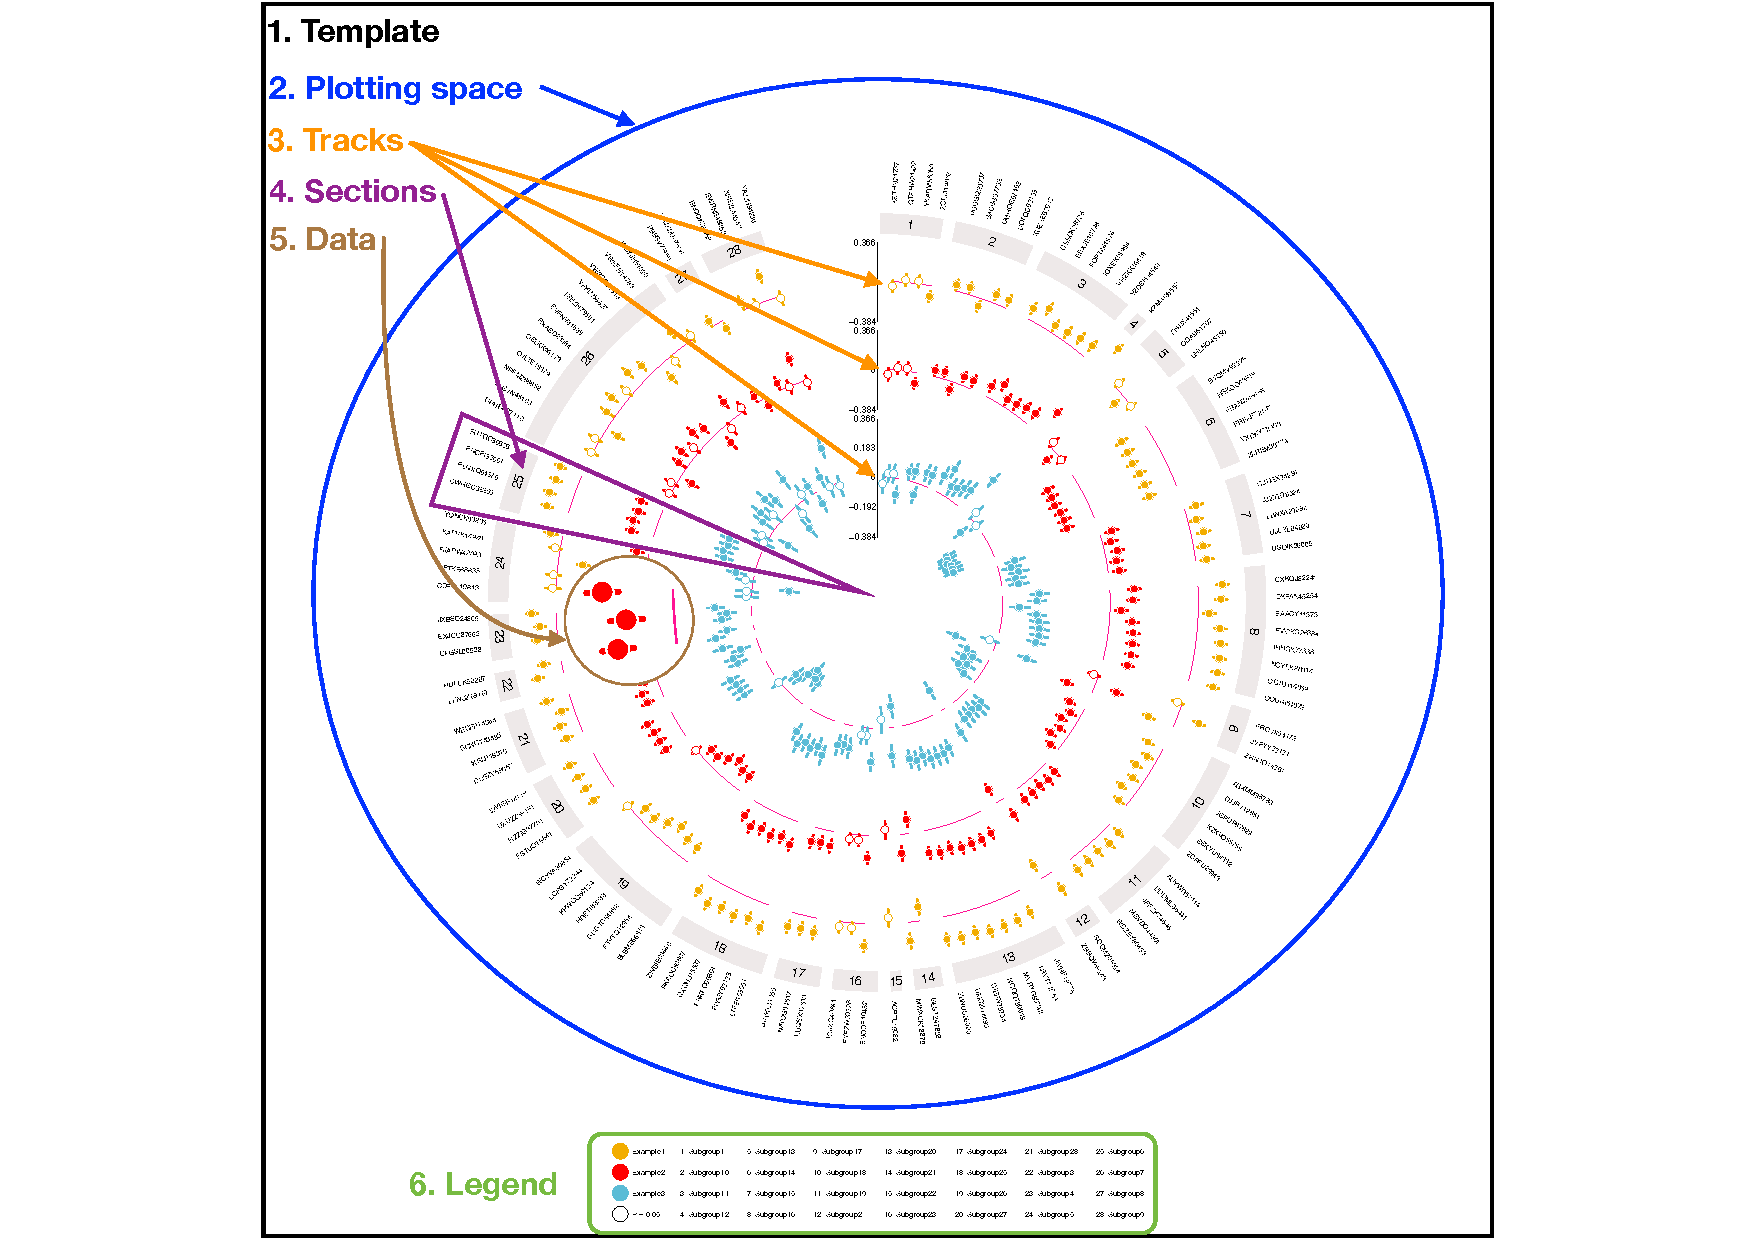
\includegraphics[width=1\linewidth]{data/chapter6/figures/annotated_circos_plot} \caption{Annotated Circos plot highlighting elements of the Circos plot}\label{fig:annotated-circos-plot}
\end{figure}
\hypertarget{implementation}{%
\subsection{Implementation}\label{implementation}}

\texttt{EpiViz} is a \texttt{Shiny} web application and \texttt{R} package. \texttt{R} (version 3.6.2)\textsuperscript{\protect\hyperlink{ref-r2019}{146}} and \texttt{Shiny}\textsuperscript{\protect\hyperlink{ref-Chang2019}{202}} (version 1.4.0) were used to develop the web application and \texttt{R} (version 3.6.2) was used to develop the \texttt{R} package. \texttt{Shiny} is an \texttt{R} package that enables development and deployment of web applications written in the \texttt{R} programming language. Development of \texttt{EpiViz} was progressive and feedback from colleagues (see Section \ref{epiviz-acknowledgements}) was vital in this process.

\hypertarget{operation}{%
\subsection{Operation}\label{operation}}

The \href{http://mrcieu.mrsoftware.org/EpiViz/}{web application} is publicly accessible -- \url{http://mrcieu.mrsoftware.org/EpiViz/} -- and held under an \href{https://github.com/mattlee821/EpiViz/blob/master/LICENSE.txt}{MIT license}. \href{https://www.docker.com/}{Docker} was used to containerise the application. The \href{http://mrcieu.mrsoftware.org/EpiViz/}{Medical Research Council Integrative Epidemiology Unit} at the University of Bristol \texttt{Shiny} server hosts the web application. The web application has been tested on computers running macOS (version 10.14) and Windows (version 10) using: Internet Explorer (version 11; Windows), Google Chrome (version 79; macOS and Windows), Safari (version 13; macOS).

The \href{https://github.com/mattlee821/EpiViz/tree/master/R_package}{\texttt{R} package} is publicly accessible through GitHub -- \url{https://github.com/mattlee821/EpiViz/tree/master/R_package} -- and held under an\href{https://github.com/mattlee821/EpiViz/blob/master/LICENSE.txt}{MIT license}. The \texttt{R} package is accessible on all computers with \texttt{R} version 3.3.0 or higher and has been tested on macOS (version 10.14) and Windows (version 10) running \texttt{R} version 3.3.0 or higher.

A legend function is available for both the web application and \texttt{R} package and is implemented using functions from the \href{https://jokergoo.github.io/ComplexHeatmap-reference/book/}{\texttt{ComplexHeatmap}}\textsuperscript{\protect\hyperlink{ref-Gu2016}{201}} \texttt{R} package. By default the colours used for the Circos plot in both the web-application and \texttt{R} package are accessible colours identified using \href{https://medialab.github.io/iwanthue/}{i want hue}. Example data is provided on the web application \emph{Home} tab and with the \texttt{R} package using the function \texttt{EpiViz::EpiViz\_data*()} where \texttt{*} is 1-3. Example data can be produced for use with the web-application and \texttt{R} package using code on \href{https://github.com/mattlee821/EpiViz/blob/master/R_package/data-raw/example_data_simulation.R}{GitHub}.

\hypertarget{shiny-web-application}{%
\subsubsection{\texorpdfstring{\texttt{Shiny} web application}{Shiny web application}}\label{shiny-web-application}}

In order to use the \href{http://mrcieu.mrsoftware.org/EpiViz/}{web application} a web-browser and an internet connection of at least 1Mbps is required. No other system requirements are needed. Upon opening the web application, users are shown a number of example Circos plots created with the application and are directed towards the \href{}{\emph{Home}} tab. The \emph{Home} tab (Figure \ref{fig:web-app-home}) provides users with a short summary of the application, link to the \texttt{R} package, and example data for use with the app.
\begin{figure}
\includegraphics[width=1\linewidth]{data/chapter6/figures/web_app_home} \caption{Screenshot of the EpiViz web application Home page}\label{fig:web-app-home}
\end{figure}
The \href{}{\emph{How to}} provides instructions for using the application and is split into three: Step 1 deals with the preparation of data to be used with the application, step 2 deals with how to use the application, and step 3 provides information on potential next steps. Users are instructed to upload one data frame per track of the Circos plot. Each data frame should be a tab delimited text file and \texttt{R} code is provided for users to achieve this. The user is guided through an example utilising the example data provided with the application and downloadable on the \emph{Home} tab.

Having prepared their data as instructed in Step 1, users select the \href{}{\emph{Analysis}} tab and upload one data frame for each track of the Circos plot. If formatted as described in the \emph{How to} tab, descriptive information including a volcano plot will be produced automatically (Figure \ref{fig:web-app-analysis-step1}).
\begin{figure}
\includegraphics[width=1\linewidth]{data/chapter6/figures/web_app_analysis_data} \caption{Screenshot of the EpiViz web application Analysis page, showing Step 1}\label{fig:web-app-analysis-step1}
\end{figure}
If the data frame appears as expected to the user the Circos plot can then be produced by selecting the \href{}{\emph{Plot}} tab. A series of drop down lists are presented which auto-populate with the column names from the first uploaded data frame. The following column information is required for the Circos plot: label, group, estimate, p-value, lower confidence interval, upper confidence interval (Figure \ref{fig:web-app-analysis-step2}). Users can select one, two, or three tracks for their Circos plot, with data for the respective track coming from the upload data section.
\begin{figure}
\includegraphics[width=1\linewidth]{data/chapter6/figures/web_app_analysis_plot} \caption{Screenshot of the EpiViz web application Analysis page, showing Step 2}\label{fig:web-app-analysis-step2}
\end{figure}
A p-value threshold (default 0.05) can be provided to indicate a significance threshold. On the Circos plot a solid point is indicated as reaching the significance threshold and an open point indicates not reaching the threshold. An optional legend function is provided and users can choose the labels for the legend points. The legend is auto-populated using the levels in the \texttt{group} column of the up-loaded data frame. Finally, users can select to use \emph{Accessible colours} (default) or \emph{Not accessible colours} for the colours of the points on the Circos plot.

\hypertarget{r-package}{%
\subsubsection{\texorpdfstring{\texttt{R} package}{R package}}\label{r-package}}

The \texttt{EpiViz} \texttt{R} package is accessed using \texttt{R} version 3.3.0 or above. Documentation for using the package to create Circos plots is available as a README on \href{https://github.com/mattlee821/EpiViz/tree/master/R_package}{GitHub} and includes use cases and troubleshooting. The \texttt{R} package can be installed directly from GitHub into \texttt{R} with the following \texttt{R} code:
\begin{Shaded}
\begin{Highlighting}[]
\CommentTok{# Install devtools}
\KeywordTok{install.packages}\NormalTok{(}\StringTok{"devtools"}\NormalTok{)}
\KeywordTok{library}\NormalTok{(devtools)}

\CommentTok{# Install directly from GitHub}
\NormalTok{devtools}\OperatorTok{::}\KeywordTok{install_github}\NormalTok{(}\StringTok{"mattlee821/EpiViz/R_package"}\NormalTok{)}
\KeywordTok{library}\NormalTok{(EpiViz)}
\end{Highlighting}
\end{Shaded}
Once installed, users can use the example data provided with the package to produce Figure \ref{fig:r-package-3-track-type-plot}, which illustrates the three different types of track available (point, line, bar), using the following \texttt{R} code:
\begin{Shaded}
\begin{Highlighting}[]
\KeywordTok{circos_plot}\NormalTok{(}\DataTypeTok{track_number =} \DecValTok{3}\NormalTok{,}
            \DataTypeTok{track1_data =}\NormalTok{ EpiViz}\OperatorTok{::}\NormalTok{EpiViz_data1,}
            \DataTypeTok{track2_data =}\NormalTok{ EpiViz}\OperatorTok{::}\NormalTok{EpiViz_data2,}
            \DataTypeTok{track3_data =}\NormalTok{ EpiViz}\OperatorTok{::}\NormalTok{EpiViz_data3,}
            \DataTypeTok{track1_type =} \StringTok{"points"}\NormalTok{,}
            \DataTypeTok{track2_type =} \StringTok{"lines"}\NormalTok{,}
            \DataTypeTok{track3_type =} \StringTok{"bar"}\NormalTok{,}
            \DataTypeTok{label_column =} \DecValTok{1}\NormalTok{,}
            \DataTypeTok{section_column =} \DecValTok{9}\NormalTok{,}
            \DataTypeTok{estimate_column =} \DecValTok{2}\NormalTok{,}
            \DataTypeTok{pvalue_column =} \DecValTok{3}\NormalTok{,}
            \DataTypeTok{pvalue_adjustment =} \DecValTok{1}\NormalTok{,}
            \DataTypeTok{lower_ci =} \DecValTok{4}\NormalTok{,}
            \DataTypeTok{upper_ci =} \DecValTok{5}\NormalTok{,}
            \DataTypeTok{lines_column =} \DecValTok{2}\NormalTok{,}
            \DataTypeTok{lines_type =} \StringTok{"o"}\NormalTok{,}
            \DataTypeTok{bar_column =} \DecValTok{2}\NormalTok{)}
\end{Highlighting}
\end{Shaded}
\begin{figure}
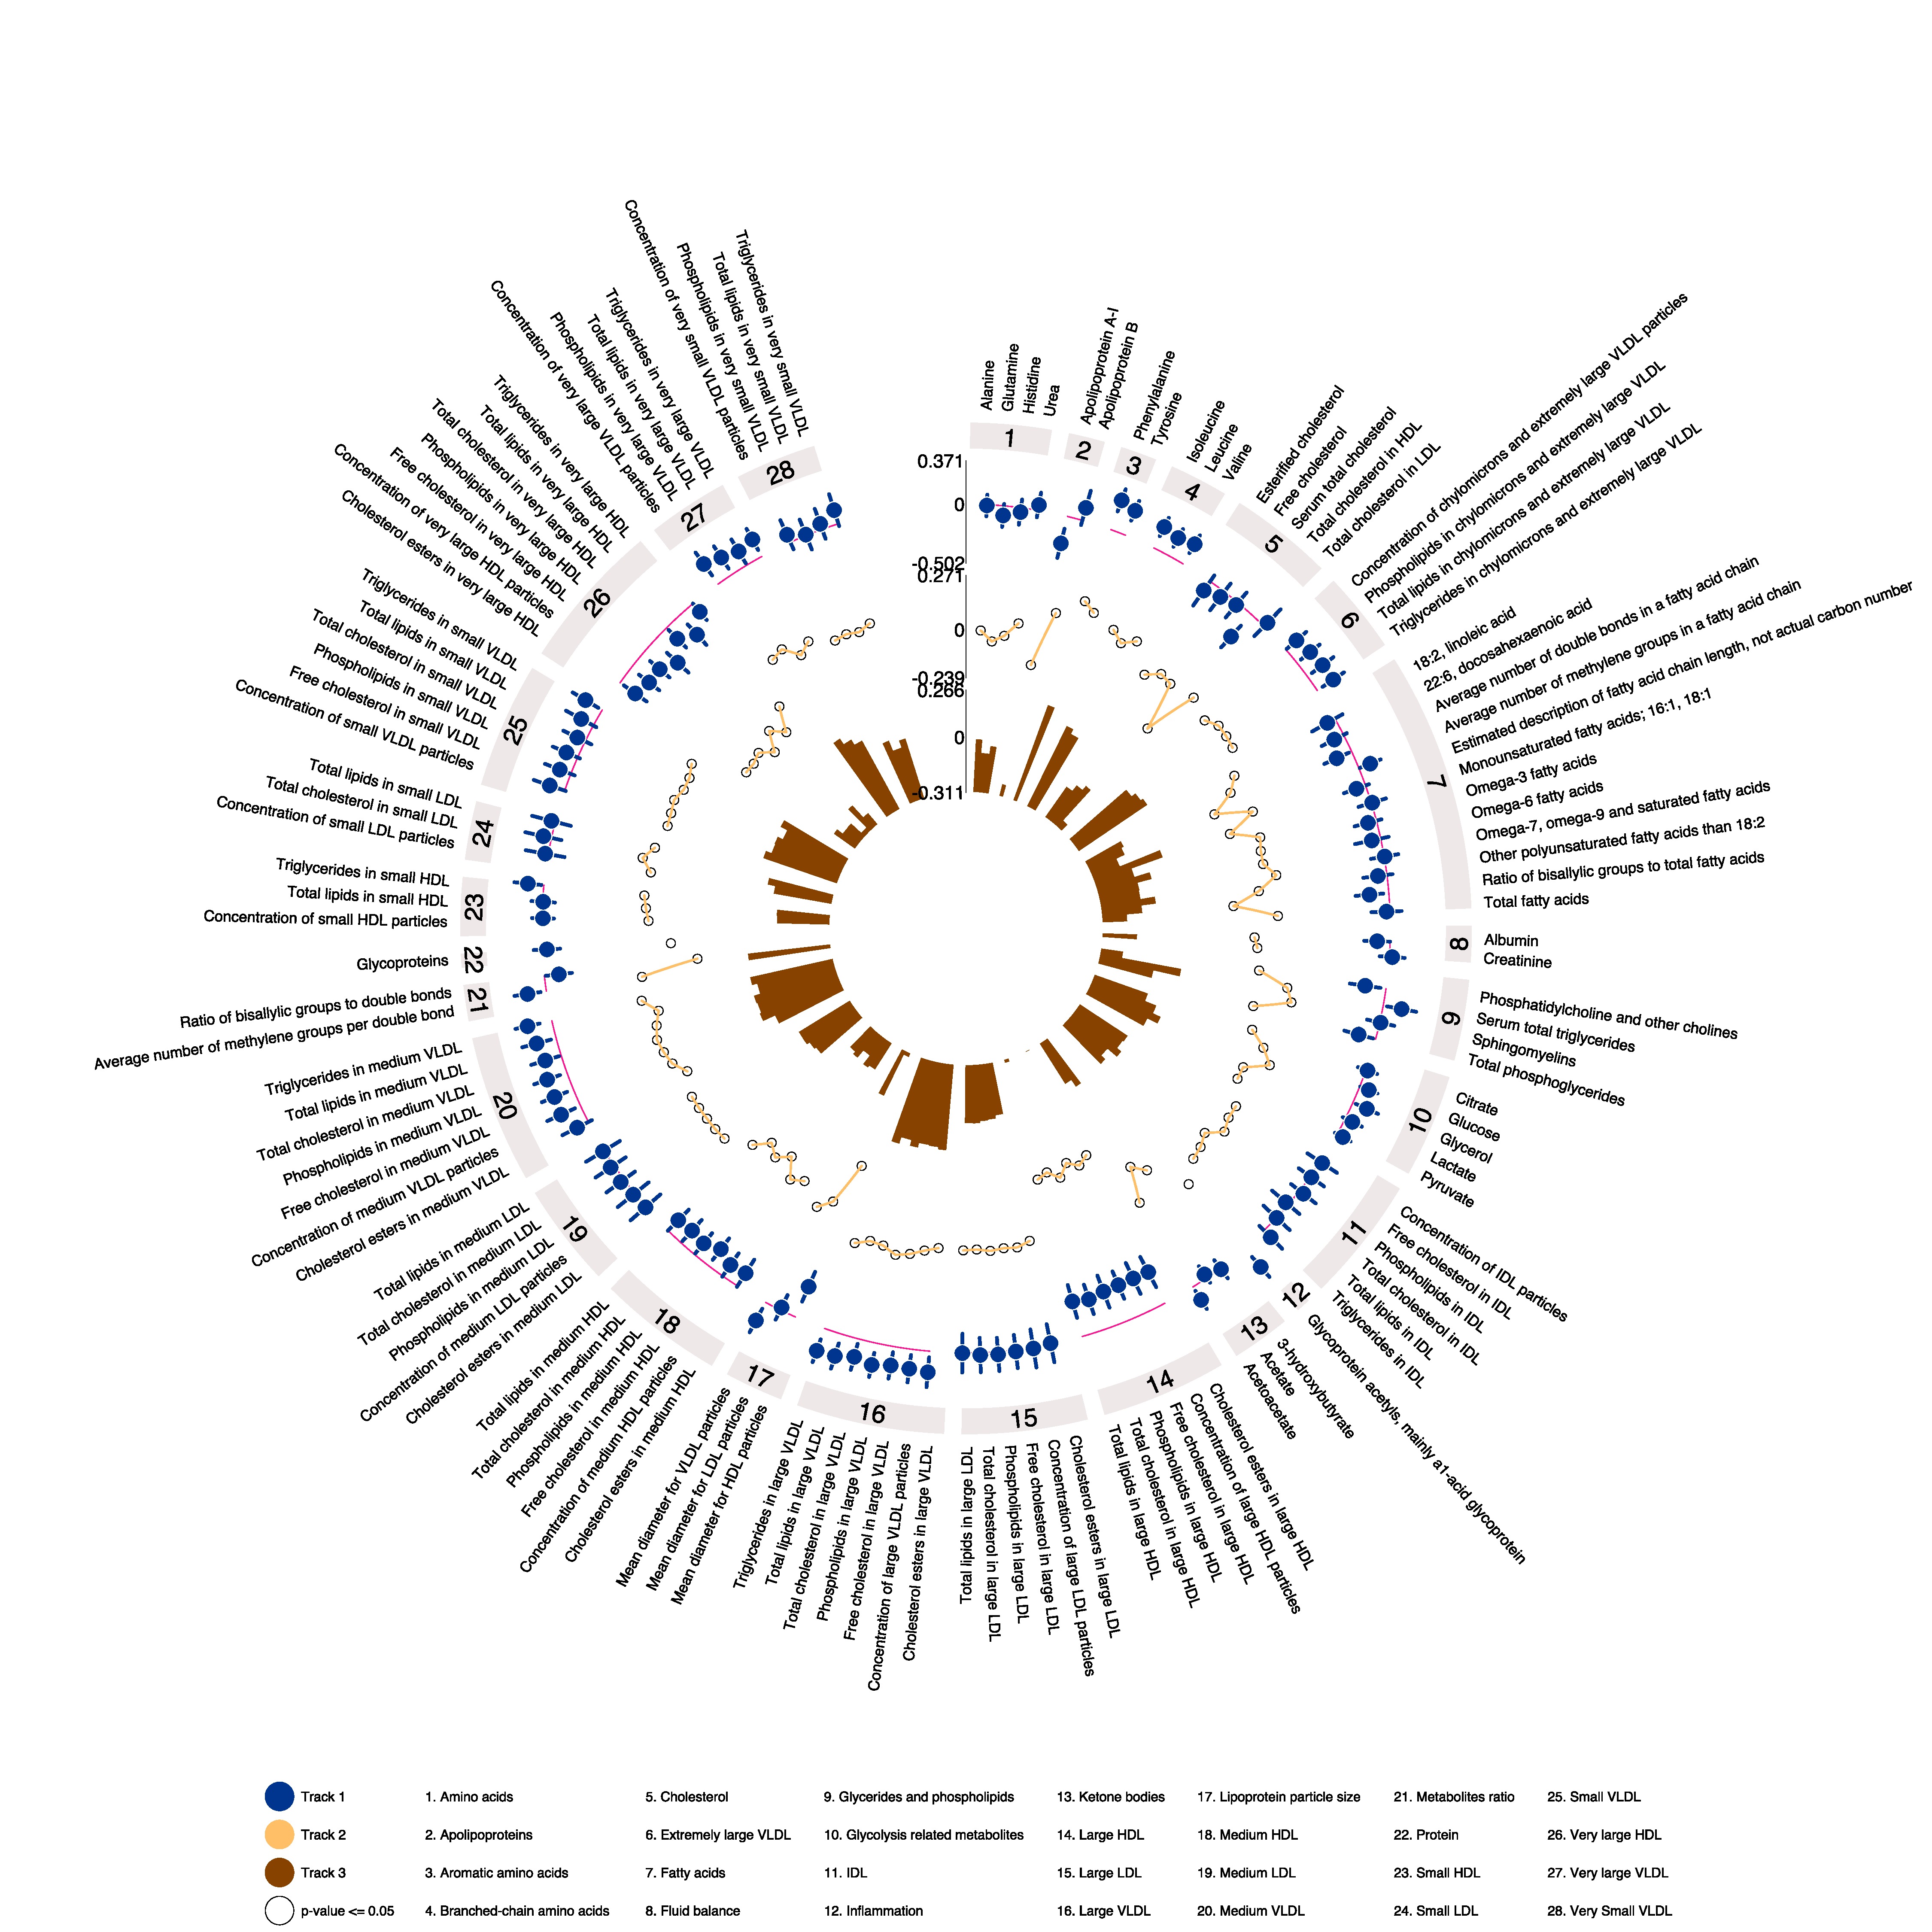
\includegraphics[width=1\linewidth]{data/chapter6/figures/r_package_3_track_type_plot} \caption{Circos plot prduced using EpiViz R package and example data}\label{fig:r-package-3-track-type-plot}
\end{figure}
These Circos plots are designed to be viewed on a screen rather than on paper. As such the plots are created at a larger scale compared to traditional plots made in \texttt{R}. This means that when viewing the Circos plot in an viewer such as the \texttt{R} Studio Viewer pane the plot appears squashed. Viewers like this should be used only as a guide when making the plot. Instead, plots should saved as \texttt{PDF} using the below code -- \texttt{PDF} files can be converted to other image formats.
\begin{Shaded}
\begin{Highlighting}[]
\KeywordTok{pdf}\NormalTok{(}\StringTok{"my_circos_plot.pdf"}\NormalTok{,}
    \DataTypeTok{width =} \DecValTok{30}\NormalTok{, }\DataTypeTok{height =} \DecValTok{30}\NormalTok{, }\DataTypeTok{pointsize =} \DecValTok{35}\NormalTok{)}
\KeywordTok{circos_plot}\NormalTok{(...}
            \DataTypeTok{circle_size =} \DecValTok{25}\NormalTok{)}
\KeywordTok{dev.off}\NormalTok{()}
\end{Highlighting}
\end{Shaded}
\texttt{R} sets default height, width and pointsize parameters and users should iterate the sizing of the plot adjusting the \texttt{width} and \texttt{height} functions to get the desired plot size. They should then adjust the \texttt{pointsize} function to increase and decrease the size of all information in the plot (labels, points, lines etc.). The numbers provided work with most plots and were used for all examples. In addition, users can adjust the size of the Circos plot directly using the argument \texttt{circle\_size}. The default for \texttt{circle\_size} is 25 and smaller numbers increase the size of the circle and larger numbers decrease the size. Finally, users can adjust the height of tracks individually using \texttt{track*\_height} where \texttt{*} refers to the track number (see below code). The default for each track is 20 percent of the total size of the circle (the section track is fixed at 5 percent).
\begin{Shaded}
\begin{Highlighting}[]
\KeywordTok{circos_plot}\NormalTok{(...}
            \DataTypeTok{track1_height =} \FloatTok{0.2}\NormalTok{,}
            \DataTypeTok{track2_height =} \FloatTok{0.2}\NormalTok{,}
            \DataTypeTok{track3_height =} \FloatTok{0.2}\NormalTok{)}
\end{Highlighting}
\end{Shaded}
In order to minimise the time required to maintain the \texttt{R} package further customisation is achieved by the users themselves. The function is written to aid this customisation with \emph{Default parameters} and \emph{Customisable parameters} located at the top of the \texttt{circos\_plot()} function script. Guidance and code is provided on \href{https://github.com/mattlee821/EpiViz/tree/master/R_package}{GitHub} to aid user customisation, for example changing track colours requires users navigating to the \emph{Customisable parameters} section and then to the \emph{Colours} section and replacing the following lines with their desired colours:
\begin{Shaded}
\begin{Highlighting}[]
\NormalTok{discrete_palette <-}\StringTok{ }\KeywordTok{c}\NormalTok{(}\StringTok{"#00378f"}\NormalTok{, }\CommentTok{# track 1 colour}
                      \StringTok{"#ffc067"}\NormalTok{, }\CommentTok{# track 2 colour}
                      \StringTok{"#894300"}\NormalTok{) }\CommentTok{# track 3 colour}
\end{Highlighting}
\end{Shaded}
\hypertarget{discussion}{%
\section{Discussion}\label{discussion}}

Circos plots have been used to visualise and provide overview of large association analyses both in the literature\textsuperscript{\protect\hyperlink{ref-Shin2014}{124},\protect\hyperlink{ref-Kettunen2016}{125}} and this thesis (see Chapters \ref{chapter4}, \ref{chapter5} and \ref{chapter9}). This has been time consuming and cumbersome. Requiring bespoke code these plots have been challenging to work with when using multiple data sets (see \href{https://github.com/mattlee821/000_thesis/tree/master/index/data/chapter6/code/circos_example.R}{GitHub} for example bespoke code).

\texttt{EpiViz} provides an efficient way to produce Circos plots for association analyses and can be implemented with little up-front cost. The web application is intended for researchers with limited to no experience of \texttt{R}, while those with some experience can gain added functionality from the \texttt{R} package. The application of Circos plots to comparing and gaining global overview of association analyses is presented in Chapters \ref{chapter4}, \ref{chapter5} and \ref{chapter9}, as well as by colleagues\textsuperscript{\protect\hyperlink{ref-Taylor2019}{193}}.

Though intended to be low maintenance, there is scope for further development of both the web application and \texttt{R} package. Of broad appeal to both is the inclusion of new plotting methods such as the chord diagram which shows relatedness between two nodes. In the case of metabolites a chord diagram would provide greater understanding about the relationship between different sections. In addition, the ability to filter and choose specific sections to display would simplify the plot and highlight potentially meaningful results.

The web application is less flexible than the \texttt{R} package, however there are specific extensions of interest. Firstly interactive plots would provide users the ability to expand sections of interest and display additional information. Rather than a final presentation of the data this would primarily focus on exploration of data. Additionally, introducing features from the \texttt{R} package such as different plot types will broaden the appeal of the web application. These additions are likely to increase the costs of maintenance however.

The \texttt{R} package has extensive scope for enhancement and presents a more efficient investment of time for extensions over the web application due to the flexibility of \texttt{R}. Currently, only a single data point can be plotted on each track at each \(X\) axis coordinate. This is to prevent over-crowding. However, if a data set has 50 points for example, adding a second point to each \(X\) axis coordinate of the track would not overcrowd the plot.

The current limited customisation afforded with the web application and the \texttt{R} package is designed to reduce the maintenance costs of the author. As a result, functions that users may wish to use, such as multiple point estimates on a single track, must be coded by the user in \texttt{R}. Though guidance is provided on GitHub for such customisations, this additional effort may reduce the utility of the tool, especially among users with little experience of \texttt{R} but very specific requirements. Similarly, although designed to be efficient, users must provide data in a specific format in order to use the web application and \texttt{R} package. \texttt{R} code is provided to aid this effort but the requirement for users with no \texttt{R} experience to create a specific data frame will be off-putting for some.

In order to achieve the desired goal of providing global overview of large association analyses Circos plots must be much larger than traditional plots such as forest plots. As such, Circos plots are best utilised as a tool for the user rather than a reader of a print journal. Circos plots are best viewed using a screen with the ability to zoom in to sections where more detail is required. This fact will reduce the utility of this type of Circos plot in publications as fixed margins will limit the size and resolution of the plot. Resolution can be improved by saving the Circos plots as a \texttt{PDF} file. Many journals do not accept \texttt{PDF} images and will convert these into lossless formats such as \texttt{PNG} or \texttt{JPEG}. This will reduce the resolution provided for readers.

\texttt{EpiViz} is simple and efficient to use. There is potential for \texttt{EpiViz} to become widely used among the community. To pre-empt popularity and provide a stable environment the web application was containerized using Docker and hosted on a server with provision for multiple-users. With popularity it is hoped that a community will help to develop \texttt{EpiViz} further.

\hypertarget{epiviz-acknowledgements}{%
\section{Acknowledgements}\label{epiviz-acknowledgements}}

\texttt{EpiViz} was greatly aided by the \texttt{R} packages \href{https://jokergoo.github.io/circlize_book/book/index.html}{\texttt{Circlize}}\textsuperscript{\protect\hyperlink{ref-Gu2014}{200}} and \href{https://jokergoo.github.io/ComplexHeatmap-reference/book/}{\texttt{ComplexHeatmap}}\textsuperscript{\protect\hyperlink{ref-Gu2016}{201}}, whose code is freely available and was used as a reference point. The following contributed to the development of \texttt{EpiViz}: Luke McGuinness, Osama Mahmoud, Sam Neaves. The following colleagues provided feedback in the development of \texttt{EpiViz}: Caroline Bull, Charlie Hatcher, Kurt Taylor, Nancy Mcbride, Neil Goulding, Steph Suddell.

\newpage

\hypertarget{chapter7}{%
\chapter{Clustering metabolites}\label{chapter7}}

\textbf{?????}

\hypertarget{chapter8}{%
\chapter{Rules for instrumenting clusters}\label{chapter8}}

\textbf{?????}

\hypertarget{chapter9}{%
\chapter{Mendelian randomization analysis: stage 2}\label{chapter9}}

\textbf{Associations between metabolites and diseases: a Mendelian randomization analysis}

\hypertarget{conclusion}{%
\chapter*{Conclusion}\label{conclusion}}
\addcontentsline{toc}{chapter}{Conclusion}

Assortative mating
\url{https://www.ncbi.nlm.nih.gov/pmc/articles/PMC6221130/\#gepi22138-bib-0017}

\appendix

\hypertarget{section}{%
\chapter{}\label{section}}

\newpage

\hypertarget{chapter1-appendix}{%
\section{Chapter 1}\label{chapter1-appendix}}

\hypertarget{literature-search}{%
\subsection{Literature search}\label{literature-search}}

Manual literature searching is prone to bias. Literature mining tools, though susceptible to publication and other biases, provide an alternative approach enabling a large number of articles to be assessed in a semi-systematic way. MELODI\textsuperscript{\protect\hyperlink{ref-Elsworth2018}{203}}, a literature mining tool, was used to identify intermediate diseases between BMI and mortality.

Briefly, MELODI creates individual article sets based on search terms (`body mass index' and `mortality') and looks for enriched overlapping terms. MELODI uses PubMed and SemMedDB to identify enriched terms. PubMed is a data base of health and biomedical research literature, and SemMedDB is a semantic predications repository built from PubMed citations. Identifying enriched overlapping terms is a two-step process. First, overlapping terms are identified. Second, the degree of overlap given the observed and expected frequency of terms across all articles not just those included in the article sets is quantified.

All articles published from 01/01/2000--09/12/2019 (maximum number of articles per article set is 1,000,000) using the terms `body mass index' as the source and `mortality' as the outcome were included. Raw results are available on \href{https://github.com/mattlee821/000_thesis/index/data/chapter1}{GitHub}. A total of 187,951 and 787,451 articles were retrieved and included in the source and outcome article sets. Using the SemMedDB Triple results a total of 10828 enriched overlapping terms were identified. This included similar terms to `body mass index' as the source, which were removed (n = 424). A Bonferroni corrected p-value (\ensuremath{1.2\times 10^{-4}}) removed 0 terms. Terms were filtered for uniqueness (n = 156) and presence in the following categories: Age Group (n = 152), Bacterium (included because of confounding with pneumonia; n = 4), finding (not an official MELODI category; n = 1), general (not an official MELODI category; n = 1), Fungus (included because of confounding with pneumonia; n = 2), Health Care Activity (n = 5), Human (n = 14), Injury or Poisoning (n = 1), Mammal (animal studies; n = 1), Patient or Disabled Group (n = 8), Population Group (n = 14), Sign or Symptom (n = 1), Virus (included because of confounding; n = 3).

The following terms were removed and merged into immunocompromised host: infections, hospital and opportunistic infections. The following terms were removed because of duplication under different names: cardiac death, sudden death, and sudden cardiac death (merged into cessation of life); coronary arteriosclerosis (atherosclerosis); cardiovascular morbidity, cardiac event, heart diseases, vascular diseases (cardiovascular diseases); depressed mood (depressive disorder); diabetes mellitus and insulin-dependent (diabetic); metabolic diseases (metabolic syndrome). The following terms were removed because they were top-level categories that could either include a wide variety of terms already included or were duplicated by other terms: chronic disease, critical illness, disability, pregnancy complications and perinatal morbidity (included in pregnancy category), pathogenesis. As a result of filtering a total of 77 terms remained. These terms were combined into 9 categories: Cancer, Cardiovascular, immune, Kidney, Liver, Neurological/behavioural, Other, Pregnancy, Respiratory. The `other' category included traits that did not fit into one of any of the other categories and which did not have aligned traits to form a separate category (Table \ref{tab:chapter1-table-MELODI}). The majority of intermediates were cardiovascular related.

It should be noted that the search did not include articles prior to the year 2000 and focussed only on those archived by PubMed. Enrichment aims to reduce the noise introduced when searching hundreds of thousands of articles, however manual curation, which will hold its own biases, is needed in order to obtain an informative list of enriched terms.
\begin{longtable}[t]{ll}
\caption{\label{tab:chapter1-table-MELODI}Intermediates between body mass index and mortality identified using the literature mining tool MELODI}\\
\toprule
Intermediate & Category\\
\midrule
Primary carcinoma of the liver cells & Cancer\\
Malignant neoplasm of stomach & Cancer\\
Malignant neoplasm of prostate & Cancer\\
Malignant neoplasm of lung & Cancer\\
Common Neoplasm & Cancer\\
\addlinespace
Liver neoplasms & Cancer\\
Malignant disease & Cancer\\
Carcinoma of the Large Intestine & Cancer\\
Pancreatic carcinoma & Cancer\\
Heart failure & Cardiovascular\\
\addlinespace
Anemia & Cardiovascular\\
Dyslipidemias & Cardiovascular\\
Cerebrovascular accident & Cardiovascular\\
Cardiovascular Diseases & Cardiovascular\\
Atherosclerosis & Cardiovascular\\
\addlinespace
Myocardial Infarction & Cardiovascular\\
Ischemic stroke & Cardiovascular\\
Acute coronary syndrome & Cardiovascular\\
Atrial Fibrillation & Cardiovascular\\
Coronary heart disease & Cardiovascular\\
\addlinespace
Systemic arterial pressure & Cardiovascular\\
Thrombosis & Cardiovascular\\
Cerebrovascular Disorders & Cardiovascular\\
Acute myocardial infarction & Cardiovascular\\
Sinus rhythm & Cardiovascular\\
\addlinespace
Cardiomyopathies & Cardiovascular\\
Myocardial Ischemia & Cardiovascular\\
Peripheral Vascular Diseases & Cardiovascular\\
Vascular calcification & Cardiovascular\\
Heart Arrest & Cardiovascular\\
\addlinespace
Myocardial rupture & Cardiovascular\\
Shock, Cardiogenic & Cardiovascular\\
Hemorrhage & Cardiovascular\\
Ischemia & Cardiovascular\\
Congestive heart failure & Cardiovascular\\
\addlinespace
Ventricular Dysfunction, Left & Cardiovascular\\
Mitral Valve Insufficiency & Cardiovascular\\
Hyperglycaemia & Cardiovascular\\
Pancreatitis & immune\\
Inflammatory disorder & immune\\
\addlinespace
Immunocompromised Host & immune\\
Bacteremia & immune\\
Septicemia & immune\\
Lupus Erythematosus, Systemic & immune\\
Sepsis Syndrome & immune\\
\addlinespace
End stage renal failure & Kidney\\
Kidney Failure, Chronic & Kidney\\
Glomerular Filtration Rate & Kidney\\
Kidney Diseases & Kidney\\
Kidney Failure & Kidney\\
\addlinespace
Renal function & Kidney\\
Liver diseases & Liver\\
Non-alcoholic fatty liver & Liver\\
Liver and Intrahepatic Biliary Tract Carcinoma & Liver\\
Chronic liver disease & Liver\\
\addlinespace
Depressive disorder & Neurological/behavioural\\
Dementia & Neurological/behavioural\\
Metabolic syndrome & Other\\
Cessation of life & Other\\
Malnutrition & Other\\
\addlinespace
Diabetic & Other\\
Multiple Organ Failure & Other\\
Fibrosis & Other\\
Deglutition Disorders & Other\\
Vitamin D Deficiency & Other\\
\addlinespace
Pre-Eclampsia & Pregnancy\\
Pregnancy & Pregnancy\\
Hypertension induced by pregnancy & Pregnancy\\
Tuberculosis & Respiratory\\
Sleep Apnea, Obstructive & Respiratory\\
\addlinespace
Pneumonia & Respiratory\\
Chronic Obstructive Airway Disease & Respiratory\\
Respiration Disorders & Respiratory\\
Respiratory Distress Syndrome, Adult & Respiratory\\
Respiratory Tract Infections & Respiratory\\
\addlinespace
Respiratory Failure & Respiratory\\
Acute respiratory failure & Respiratory\\
\bottomrule
\end{longtable}
\newpage

\hypertarget{chapter2-appendix}{%
\section{Chapter 2}\label{chapter2-appendix}}

\newpage

\hypertarget{chapter3-appendix}{%
\section{Chapter 3}\label{chapter3-appendix}}

\newpage

\hypertarget{chapter4-appendix}{%
\section{Chapter 4}\label{chapter4-appendix}}

\hypertarget{chapter4-appendix-metabolites}{%
\subsection{Metabolites}\label{chapter4-appendix-metabolites}}

\blandscape
\begin{longtabu} to \linewidth {>{\raggedright}X>{\raggedright}X>{\raggedright}X>{\raggedright}X>{\raggedright}X}
\caption{\label{tab:unnamed-chunk-35}Metabolites available after quality control across all age groups}\\
\toprule
Metabolite & Label & Class & Subclass & Derived\\
\midrule
xsvldlcepct & Cholesterol esters in very small VLDL to total lipids in very small VLDL ratio (\%) &  &  & \\
\cmidrule{1-2}
xsvldlcpct & Total cholesterol in very small VLDL to total lipids in very small VLDL ratio (\%) &  &  & \\
\cmidrule{1-2}
xsvldlfcpct & Free cholesterol in very small VLDL to total lipids in very small VLDL ratio (\%) &  &  & \\
\cmidrule{1-2}
xsvldlplpct & Phospholipids in very small VLDL to total lipids in very small VLDL ratio (\%) &  &  & \\
\cmidrule{1-2}
xsvldltgpct & Triglycerides in very small VLDL to total lipids in very small VLDL ratio (\%) &  & \multirow{-5}{*}{\raggedright\arraybackslash Very Small VLDL ratios} & \\
\cmidrule{1-2}
\cmidrule{4-4}
svldlcepct & Cholesterol esters in small VLDL to total lipids in small VLDL ratio (\%) &  &  & \\
\cmidrule{1-2}
svldlcpct & Total cholesterol in small VLDL to total lipids in small VLDL ratio (\%) &  &  & \\
\cmidrule{1-2}
svldlfcpct & Free cholesterol in small VLDL to total lipids in small VLDL ratio (\%) &  &  & \\
\cmidrule{1-2}
svldlplpct & Phospholipids in small VLDL to total lipids in small VLDL ratio (\%) &  &  & \\
\cmidrule{1-2}
svldltgpct & Triglycerides in small VLDL  to total lipids in small VLDL ratio (\%) &  & \multirow{-5}{*}{\raggedright\arraybackslash Small VLDL ratios} & \\
\cmidrule{1-2}
\cmidrule{4-4}
mvldlcepct & Cholesterol esters in medium VLDL to total lipids in medium VLDL ratio (\%) &  &  & \\
\cmidrule{1-2}
mvldlcpct & Total cholesterol in medium VLDL to total lipids in medium VLDL ratio (\%) &  &  & \\
\cmidrule{1-2}
mvldlfcpct & Free cholesterol in medium VLDL to total lipids in medium VLDL ratio (\%) &  &  & \\
\cmidrule{1-2}
mvldlplpct & Phospholipids in medium VLDL to total lipids in medium VLDL ratio (\%) &  &  & \\
\cmidrule{1-2}
mvldltgpct & Triglycerides in medium VLDL to total lipids in medium VLDL ratio (\%) &  & \multirow{-5}{*}{\raggedright\arraybackslash Medium VLDL ratios} & \\
\cmidrule{1-2}
\cmidrule{4-4}
lvldlcepct & Cholesterol esters in large VLDL to total lipids in large VLDL ratio (\%) &  &  & \\
\cmidrule{1-2}
lvldlcpct & Total cholesterol in large VLDL to total lipids in large VLDL ratio (\%) &  &  & \\
\cmidrule{1-2}
lvldlfcpct & Free cholesterol in large VLDL to total lipids in large VLDL ratio (\%) &  &  & \\
\cmidrule{1-2}
lvldlplpct & Phospholipids in large VLDL to total lipids in large VLDL ratio (\%) &  &  & \\
\cmidrule{1-2}
lvldltgpct & Triglycerides in large VLDL to total lipids in large VLDL ratio (\%) &  & \multirow{-5}{*}{\raggedright\arraybackslash Large VLDL ratios} & \\
\cmidrule{1-2}
\cmidrule{4-4}
xlvldlcepct & Cholesterol esters in very large VLDL to total lipids in very large VLDL ratio (\%) &  &  & \\
\cmidrule{1-2}
xlvldlcpct & Total cholesterol in very large VLDL to total lipids in very large VLDL ratio (\%) &  &  & \\
\cmidrule{1-2}
xlvldlfcpct & Free cholesterol in very large VLDL to total lipids in very large VLDL ratio (\%) &  &  & \\
\cmidrule{1-2}
xlvldlplpct & Phospholipids in very large VLDL to total lipids in very large VLDL ratio (\%) &  &  & \\
\cmidrule{1-2}
xlvldltgpct & Triglycerides in very large VLDL to total lipids in very large VLDL ratio (\%) &  & \multirow{-5}{*}{\raggedright\arraybackslash Very large VLDL ratios} & \\
\cmidrule{1-2}
\cmidrule{4-4}
xxlvldlcepct & Cholesterol esters in chylomicrons and extremely large VLDL to total lipids in chylomicrons and extremely large VLDL ratio (\%) &  &  & \\
\cmidrule{1-2}
xxlvldlcpct & Total cholesterol in chylomicrons and extremely large VLDL to total lipids in chylomicrons and extremely large VLDL ratio (\%) &  &  & \\
\cmidrule{1-2}
xxlvldlfcpct & Free cholesterol in chylomicrons and extremely large VLDL to total lipids in chylomicrons and extremely large VLDL ratio (\%) &  &  & \\
\cmidrule{1-2}
xxlvldlplpct & Phospholipids in chylomicrons and extremely large VLDL to total lipids in chylomicrons and extremely large VLDL ratio (\%) &  &  & \\
\cmidrule{1-2}
xxlvldltgpct & Triglycerides in chylomicrons and extremely large VLDL to total lipids in chylomicrons and extremely large VLDL ratio (\%) &  & \multirow{-5}{*}{\raggedright\arraybackslash Extremely large VLDL ratios} & \\
\cmidrule{1-2}
\cmidrule{4-4}
idlcepct & Cholesterol esters in IDL to total lipids in IDL ratio (\%) &  &  & \\
\cmidrule{1-2}
idlcpct & Total cholesterol in IDL to total lipids in IDL ratio (\%) &  &  & \\
\cmidrule{1-2}
idlfcpct & Free cholesterol in IDL to total lipids in IDL ratio (\%) &  &  & \\
\cmidrule{1-2}
idlplpct & Phospholipids in IDL to total lipids in IDL ratio (\%) &  &  & \\
\cmidrule{1-2}
idltgpct & Triglycerides in IDL to total lipids in IDL ratio (\%) &  & \multirow{-5}{*}{\raggedright\arraybackslash IDL ratios} & \\
\cmidrule{1-2}
\cmidrule{4-4}
sldlcepct & Cholesterol esters in small LDL to total lipids in small LDL ratio (\%) &  &  & \\
\cmidrule{1-2}
sldlcpct & Total cholesterol in small LDL to total lipids in small LDL ratio (\%) &  &  & \\
\cmidrule{1-2}
sldlfcpct & Free cholesterol in small LDL to total lipids in small LDL ratio (\%) &  &  & \\
\cmidrule{1-2}
sldlplpct & Phospholipids in small LDL to total lipids in small LDL ratio (\%) &  &  & \\
\cmidrule{1-2}
sldltgpct & Triglycerides in small LDL to total lipids in small LDL ratio (\%) &  & \multirow{-5}{*}{\raggedright\arraybackslash Small LDL ratios} & \\
\cmidrule{1-2}
\cmidrule{4-4}
mldlcepct & Cholesterol esters in medium LDL to total lipids in medium LDL ratio (\%) &  &  & \\
\cmidrule{1-2}
mldlcpct & Total cholesterol in medium LDL to total lipids in medium LDL ratio (\%) &  &  & \\
\cmidrule{1-2}
mldlfcpct & Free cholesterol in medium LDL to total lipids in medium LDL ratio (\%) &  &  & \\
\cmidrule{1-2}
mldlplpct & Phospholipids in medium LDL to total lipids in medium LDL ratio (\%) &  &  & \\
\cmidrule{1-2}
mldltgpct & Triglycerides in medium LDL to total lipids in medium LDL ratio (\%) &  & \multirow{-5}{*}{\raggedright\arraybackslash Medium LDL ratios} & \\
\cmidrule{1-2}
\cmidrule{4-4}
lldlcepct & Cholesterol esters in large LDL to total lipids in large LDL ratio (\%) &  &  & \\
\cmidrule{1-2}
lldlcpct & Total cholesterol in large LDL to total lipids in large LDL ratio (\%) &  &  & \\
\cmidrule{1-2}
lldlfcpct & Free cholesterol in large LDL to total lipids in large LDL ratio (\%) &  &  & \\
\cmidrule{1-2}
lldlplpct & Phospholipids in large LDL to total lipids in large LDL ratio (\%) &  &  & \\
\cmidrule{1-2}
lldltgpct & Triglycerides in large LDL to total lipids in large LDL ratio (\%) &  & \multirow{-5}{*}{\raggedright\arraybackslash Large LDL ratios} & \\
\cmidrule{1-2}
\cmidrule{4-4}
shdlcepct & Cholesterol esters in small HDL to total lipids in small HDL ratio (\%) &  &  & \\
\cmidrule{1-2}
shdlcpct & Total cholesterol in small HDL to total lipids in small HDL ratio (\%) &  &  & \\
\cmidrule{1-2}
shdlfcpct & Free cholesterol in small HDL to total lipids in small HDL ratio (\%) &  &  & \\
\cmidrule{1-2}
shdlplpct & Phospholipids in small HDL to total lipids in small HDL ratio (\%) &  &  & \\
\cmidrule{1-2}
shdltgpct & Triglycerides in small HDL to total lipids in small HDL ratio (\%) &  & \multirow{-5}{*}{\raggedright\arraybackslash Small HDL ratios} & \\
\cmidrule{1-2}
\cmidrule{4-4}
mhdlcepct & Cholesterol esters in medium HDL to total lipids in medium HDL ratio (\%) &  &  & \\
\cmidrule{1-2}
mhdlcpct & Total cholesterol in medium HDL to total lipids in medium HDL ratio (\%) &  &  & \\
\cmidrule{1-2}
mhdlfcpct & Free cholesterol in medium HDL to total lipids in medium HDL ratio (\%) &  &  & \\
\cmidrule{1-2}
mhdlplpct & Phospholipids in medium HDL to total lipids in medium HDL ratio (\%) &  &  & \\
\cmidrule{1-2}
mhdltgpct & Triglycerides in medium HDL to total lipids in medium HDL ratio (\%) &  & \multirow{-5}{*}{\raggedright\arraybackslash Medium HDL ratios} & \\
\cmidrule{1-2}
\cmidrule{4-4}
lhdlcepct & Cholesterol esters in large HDL to total lipids in large HDL ratio (\%) &  &  & \\
\cmidrule{1-2}
lhdlcpct & Total cholesterol in large HDL to total lipids in large HDL ratio (\%) &  &  & \\
\cmidrule{1-2}
lhdlfcpct & Free cholesterol in large HDL to total lipids in large HDL ratio (\%) &  &  & \\
\cmidrule{1-2}
lhdlplpct & Phospholipids in large HDL to total lipids in large HDL ratio (\%) &  &  & \\
\cmidrule{1-2}
lhdltgpct & Triglycerides in large HDL to total lipids in large HDL ratio (\%) &  & \multirow{-5}{*}{\raggedright\arraybackslash Large HDL ratios} & \\
\cmidrule{1-2}
\cmidrule{4-4}
xlhdlcepct & Cholesterol esters in very large HDL to total lipids in very large HDL ratio (\%) &  &  & \\
\cmidrule{1-2}
xlhdlcpct & Total cholesterol in very large HDL to total lipids in very large HDL ratio (\%) &  &  & \\
\cmidrule{1-2}
xlhdlfcpct & Free cholesterol in very large HDL to total lipids in very large HDL ratio (\%) &  &  & \\
\cmidrule{1-2}
xlhdlplpct & Phospholipids in very large HDL to total lipids in very large HDL ratio (\%) &  &  & \\
\cmidrule{1-2}
xlhdltgpct & Triglycerides in very large HDL to total lipids in very large HDL ratio (\%) & \multirow{-70}{*}{\raggedright\arraybackslash Lipoprotein subclasses ratios} & \multirow{-5}{*}{\raggedright\arraybackslash Very large HDL ratios} & \multirow{-70}{*}{\raggedright\arraybackslash yes}\\
\cmidrule{1-5}
xsvldlc & Total cholesterol in very small VLDL (mmol/l) &  &  & \\
\cmidrule{1-2}
xsvldlce & Cholesterol esters in very small VLDL (mmol/l) &  &  & \\
\cmidrule{1-2}
xsvldlfc & Free cholesterol in very small VLDL (mmol/l) &  &  & \\
\cmidrule{1-2}
xsvldll & Total lipids in very small VLDL (mmol/l) &  &  & \\
\cmidrule{1-2}
xsvldlp & Concentration of very small VLDL particles (mol/l) &  &  & \\
\cmidrule{1-2}
xsvldlpl & Phospholipids in very small VLDL (mmol/l) &  &  & \\
\cmidrule{1-2}
xsvldltg & Triglycerides in very small VLDL (mmol/l) &  & \multirow{-7}{*}{\raggedright\arraybackslash Very Small VLDL} & \\
\cmidrule{1-2}
\cmidrule{4-4}
svldlc & Total cholesterol in small VLDL (mmol/l) &  &  & \\
\cmidrule{1-2}
svldlce & Cholesterol esters in small VLDL (mmol/l) &  &  & \\
\cmidrule{1-2}
svldlfc & Free cholesterol in small VLDL (mmol/l) &  &  & \\
\cmidrule{1-2}
svldll & Total lipids in small VLDL (mmol/l) &  &  & \\
\cmidrule{1-2}
svldlp & Concentration of small VLDL particles (mol/l) &  &  & \\
\cmidrule{1-2}
svldlpl & Phospholipids in small VLDL (mmol/l) &  &  & \\
\cmidrule{1-2}
svldltg & Triglycerides in small VLDL (mmol/l) &  & \multirow{-7}{*}{\raggedright\arraybackslash Small VLDL} & \\
\cmidrule{1-2}
\cmidrule{4-4}
mvldlc & Total cholesterol in medium VLDL (mmol/l) &  &  & \\
\cmidrule{1-2}
mvldlce & Cholesterol esters in medium VLDL (mmol/l) &  &  & \\
\cmidrule{1-2}
mvldlfc & Free cholesterol in medium VLDL (mmol/l) &  &  & \\
\cmidrule{1-2}
mvldll & Total lipids in medium VLDL (mmol/l) &  &  & \\
\cmidrule{1-2}
mvldlp & Concentration of medium VLDL particles (mol/l) &  &  & \\
\cmidrule{1-2}
mvldlpl & Phospholipids in medium VLDL (mmol/l) &  &  & \\
\cmidrule{1-2}
mvldltg & Triglycerides in medium VLDL (mmol/l) &  & \multirow{-7}{*}{\raggedright\arraybackslash Medium VLDL} & \\
\cmidrule{1-2}
\cmidrule{4-4}
lvldlc & Total cholesterol in large VLDL (mmol/l) &  &  & \\
\cmidrule{1-2}
lvldlce & Cholesterol esters in large VLDL (mmol/l) &  &  & \\
\cmidrule{1-2}
lvldlfc & Free cholesterol in large VLDL (mmol/l) &  &  & \\
\cmidrule{1-2}
lvldll & Total lipids in large VLDL (mmol/l) &  &  & \\
\cmidrule{1-2}
lvldlp & Concentration of large VLDL particles (mol/l) &  &  & \\
\cmidrule{1-2}
lvldlpl & Phospholipids in large VLDL (mmol/l) &  &  & \\
\cmidrule{1-2}
lvldltg & Triglycerides in large VLDL (mmol/l) &  & \multirow{-7}{*}{\raggedright\arraybackslash Large VLDL} & \\
\cmidrule{1-2}
\cmidrule{4-4}
xlvldlc & Total cholesterol in very large VLDL (mmol/l) &  &  & \\
\cmidrule{1-2}
xlvldlce & Cholesterol esters in very large VLDL (mmol/l) &  &  & \\
\cmidrule{1-2}
xlvldlfc & Free cholesterol in very large VLDL (mmol/l) &  &  & \\
\cmidrule{1-2}
xlvldll & Total lipids in very large VLDL (mmol/l) &  &  & \\
\cmidrule{1-2}
xlvldlp & Concentration of very large VLDL particles (mol/l) &  &  & \\
\cmidrule{1-2}
xlvldlpl & Phospholipids in very large VLDL (mmol/l) &  &  & \\
\cmidrule{1-2}
xlvldltg & Triglycerides in very large VLDL (mmol/l) &  & \multirow{-7}{*}{\raggedright\arraybackslash Very large VLDL} & \\
\cmidrule{1-2}
\cmidrule{4-4}
xxlvldlc & Total cholesterol in chylomicrons and extremely large VLDL (mmol/l) &  &  & \\
\cmidrule{1-2}
xxlvldlce & Cholesterol esters in chylomicrons and extremely large VLDL (mmol/l) &  &  & \\
\cmidrule{1-2}
xxlvldlfc & Free cholesterol in chylomicrons and extremely large VLDL (mmol/l) &  &  & \\
\cmidrule{1-2}
xxlvldll & Total lipids in chylomicrons and extremely large VLDL (mmol/l) &  &  & \\
\cmidrule{1-2}
xxlvldlp & Concentration of chylomicrons and extremely large VLDL particles (mol/l) &  &  & \\
\cmidrule{1-2}
xxlvldlpl & Phospholipids in chylomicrons and extremely large VLDL (mmol/l) &  &  & \\
\cmidrule{1-2}
xxlvldltg & Triglycerides in chylomicrons and extremely large VLDL (mmol/l) &  & \multirow{-7}{*}{\raggedright\arraybackslash Extremely large VLDL} & \\
\cmidrule{1-2}
\cmidrule{4-4}
idlc & Total cholesterol in IDL (mmol/l) &  &  & \\
\cmidrule{1-2}
idlce & Cholesterol esters in IDL (mmol/l) &  &  & \\
\cmidrule{1-2}
idlfc & Free cholesterol in IDL (mmol/l) &  &  & \\
\cmidrule{1-2}
idll & Total lipids in IDL (mmol/l) &  &  & \\
\cmidrule{1-2}
idlp & Concentration of IDL particles (mol/l) &  &  & \\
\cmidrule{1-2}
idlpl & Phospholipids in IDL (mmol/l) &  &  & \\
\cmidrule{1-2}
idltg & Triglycerides in IDL (mmol/l) &  & \multirow{-7}{*}{\raggedright\arraybackslash IDL} & \\
\cmidrule{1-2}
\cmidrule{4-4}
sldlc & Total cholesterol in small LDL (mmol/l) &  &  & \\
\cmidrule{1-2}
sldlce & Cholesterol esters in small LDL (mmol/l) &  &  & \\
\cmidrule{1-2}
sldlfc & Free cholesterol in small LDL (mmol/l) &  &  & \\
\cmidrule{1-2}
sldll & Total lipids in small LDL (mmol/l) &  &  & \\
\cmidrule{1-2}
sldlp & Concentration of small LDL particles (mol/l) &  &  & \\
\cmidrule{1-2}
sldlpl & Phospholipids in small LDL (mmol/l) &  &  & \\
\cmidrule{1-2}
sldltg & Triglycerides in small LDL (mmol/l) &  & \multirow{-7}{*}{\raggedright\arraybackslash Small LDL} & \\
\cmidrule{1-2}
\cmidrule{4-4}
mldlc & Total cholesterol in medium LDL (mmol/l) &  &  & \\
\cmidrule{1-2}
mldlce & Cholesterol esters in medium LDL (mmol/l) &  &  & \\
\cmidrule{1-2}
mldlfc & Free cholesterol in medium LDL (mmol/l) &  &  & \\
\cmidrule{1-2}
mldll & Total lipids in medium LDL (mmol/l) &  &  & \\
\cmidrule{1-2}
mldlp & Concentration of medium LDL particles (mol/l) &  &  & \\
\cmidrule{1-2}
mldlpl & Phospholipids in medium LDL (mmol/l) &  &  & \\
\cmidrule{1-2}
mldltg & Triglycerides in medium LDL (mmol/l) &  & \multirow{-7}{*}{\raggedright\arraybackslash Medium LDL} & \\
\cmidrule{1-2}
\cmidrule{4-4}
lldlc & Total cholesterol in large LDL (mmol/l) &  &  & \\
\cmidrule{1-2}
lldlce & Cholesterol esters in large LDL (mmol/l) &  &  & \\
\cmidrule{1-2}
lldlfc & Free cholesterol in large LDL (mmol/l) &  &  & \\
\cmidrule{1-2}
lldll & Total lipids in large LDL (mmol/l) &  &  & \\
\cmidrule{1-2}
lldlp & Concentration of large LDL particles (mol/l) &  &  & \\
\cmidrule{1-2}
lldlpl & Phospholipids in large LDL (mmol/l) &  &  & \\
\cmidrule{1-2}
lldltg & Triglycerides in large LDL (mmol/l) &  & \multirow{-7}{*}{\raggedright\arraybackslash Large LDL} & \\
\cmidrule{1-2}
\cmidrule{4-4}
shdlc & Total cholesterol in small HDL (mmol/l) &  &  & \\
\cmidrule{1-2}
shdlce & Cholesterol esters in small HDL (mmol/l) &  &  & \\
\cmidrule{1-2}
shdlfc & Free cholesterol in small HDL (mmol/l) &  &  & \\
\cmidrule{1-2}
shdll & Total lipids in small HDL (mmol/l) &  &  & \\
\cmidrule{1-2}
shdlp & Concentration of small HDL particles (mol/l) &  &  & \\
\cmidrule{1-2}
shdlpl & Phospholipids in small HDL (mmol/l) &  &  & \\
\cmidrule{1-2}
shdltg & Triglycerides in small HDL (mmol/l) &  & \multirow{-7}{*}{\raggedright\arraybackslash Small HDL} & \\
\cmidrule{1-2}
\cmidrule{4-4}
mhdlc & Total cholesterol in medium HDL (mmol/l) &  &  & \\
\cmidrule{1-2}
mhdlce & Cholesterol esters in medium HDL (mmol/l) &  &  & \\
\cmidrule{1-2}
mhdlfc & Free cholesterol in medium HDL (mmol/l) &  &  & \\
\cmidrule{1-2}
mhdll & Total lipids in medium HDL (mmol/l) &  &  & \\
\cmidrule{1-2}
mhdlp & Concentration of medium HDL particles (mol/l) &  &  & \\
\cmidrule{1-2}
mhdlpl & Phospholipids in medium HDL (mmol/l) &  &  & \\
\cmidrule{1-2}
mhdltg & Triglycerides in medium HDL (mmol/l) &  & \multirow{-7}{*}{\raggedright\arraybackslash Medium HDL} & \\
\cmidrule{1-2}
\cmidrule{4-4}
lhdlc & Total cholesterol in large HDL (mmol/l) &  &  & \\
\cmidrule{1-2}
lhdlce & Cholesterol esters in large HDL (mmol/l) &  &  & \\
\cmidrule{1-2}
lhdlfc & Free cholesterol in large HDL (mmol/l) &  &  & \\
\cmidrule{1-2}
lhdll & Total lipids in large HDL (mmol/l) &  &  & \\
\cmidrule{1-2}
lhdlp & Concentration of large HDL particles (mol/l) &  &  & \\
\cmidrule{1-2}
lhdlpl & Phospholipids in large HDL (mmol/l) &  &  & \\
\cmidrule{1-2}
lhdltg & Triglycerides in large HDL (mmol/l) &  & \multirow{-7}{*}{\raggedright\arraybackslash Large HDL} & \\
\cmidrule{1-2}
\cmidrule{4-4}
xlhdlc & Total cholesterol in very large HDL (mmol/l) &  &  & \\
\cmidrule{1-2}
xlhdlce & Cholesterol esters in very large HDL (mmol/l) &  &  & \\
\cmidrule{1-2}
xlhdlfc & Free cholesterol in very large HDL (mmol/l) &  &  & \\
\cmidrule{1-2}
xlhdll & Total lipids in very large HDL (mmol/l) &  &  & \\
\cmidrule{1-2}
xlhdlp & Concentration of very large HDL particles (mol/l) &  &  & \\
\cmidrule{1-2}
xlhdlpl & Phospholipids in very large HDL (mmol/l) &  &  & \\
\cmidrule{1-2}
xlhdltg & Triglycerides in very large HDL (mmol/l) & \multirow{-98}{*}{\raggedright\arraybackslash Lipoprotein subclasses} & \multirow{-7}{*}{\raggedright\arraybackslash Very large HDL} & \\
\cmidrule{1-4}
hdld & Mean diameter for HDL particles (nm) &  &  & \\
\cmidrule{1-2}
ldld & Mean diameter for LDL particles (nm) &  &  & \\
\cmidrule{1-2}
vldld & Mean diameter for VLDL particles (nm) & \multirow{-3}{*}{\raggedright\arraybackslash Lipoprotein particle size} & \multirow{-3}{*}{\raggedright\arraybackslash Lipoprotein particle size} & \\
\cmidrule{1-4}
acace & Acetoacetate (mmol/l) &  &  & \\
\cmidrule{1-2}
ace & Acetate (mmol/l) &  &  & \\
\cmidrule{1-2}
bohbut & 3-hydroxybutyrate (mmol/l) & \multirow{-3}{*}{\raggedright\arraybackslash Ketone bodies} & \multirow{-3}{*}{\raggedright\arraybackslash Ketone bodies} & \\
\cmidrule{1-4}
gp & Glycoprotein acetyls, mainly a1-acid glycoprotein (mmol/l) & Inflammation & Inflammation & \\
\cmidrule{1-4}
cit & Citrate (mmol/l) &  &  & \\
\cmidrule{1-2}
glc & Glucose (mmol/l) &  &  & \\
\cmidrule{1-2}
lac & Lactate (mmol/l) &  &  & \\
\cmidrule{1-2}
pyr & Pyruvate (mmol/l) & \multirow{-4}{*}{\raggedright\arraybackslash Glycolysis related metabolites} & \multirow{-4}{*}{\raggedright\arraybackslash Glycolysis related metabolites} & \\
\cmidrule{1-4}
dag & Diacylglycerol (mmol/l) &  &  & \\
\cmidrule{1-2}
hdltg & Triglycerides in HDL (mmol/l) &  &  & \\
\cmidrule{1-2}
ldltg & Triglycerides in LDL (mmol/l) &  &  & \\
\cmidrule{1-2}
pc & Phosphatidylcholine and other cholines (mmol/l) &  &  & \\
\cmidrule{1-2}
serumtg & Serum total triglycerides (mmol/l) &  &  & \\
\cmidrule{1-2}
sm & Sphingomyelins (mmol/l) &  &  & \\
\cmidrule{1-2}
totcho & Total cholines (mmol/l) &  &  & \\
\cmidrule{1-2}
totpg & Total phosphoglycerides (mmol/l) &  &  & \\
\cmidrule{1-2}
vldltg & Triglycerides in VLDL (mmol/l) & \multirow{-9}{*}{\raggedright\arraybackslash Glycerides and phospholipids} & \multirow{-9}{*}{\raggedright\arraybackslash Glycerides and phospholipids} & \\
\cmidrule{1-4}
alb & Albumin  (signal area) &  &  & \\
\cmidrule{1-2}
crea & Creatinine (mmol/l) & \multirow{-2}{*}{\raggedright\arraybackslash Fluid balance} & \multirow{-2}{*}{\raggedright\arraybackslash Fluid balance} & \multirow{-120}{*}{\raggedright\arraybackslash no}\\
\cmidrule{1-5}
clafa & Ratio of conjugated linoleic acid to total fatty acids (\%) &  &  & \\
\cmidrule{1-2}
dhafa & Ratio of 22:6 docosahexaenoic acid to total fatty acids (\%) &  &  & \\
\cmidrule{1-2}
faw3fa & Ratio of omega-3 fatty acids to total fatty acids (\%) &  &  & \\
\cmidrule{1-2}
faw6fa & Ratio of omega-6 fatty acids to total fatty acids (\%) &  &  & \\
\cmidrule{1-2}
lafa & Ratio of 18:2 linoleic acid to total fatty acids (\%) &  &  & \\
\cmidrule{1-2}
mufafa & Ratio of monounsaturated fatty acids to total fatty acids (\%) &  &  & \\
\cmidrule{1-2}
pufafa & Ratio of polyunsaturated fatty acids to total fatty acids (\%) &  &  & \\
\cmidrule{1-2}
sfafa & Ratio of saturated fatty acids to total fatty acids (\%) & \multirow{-8}{*}{\raggedright\arraybackslash Fatty acids ratios} & \multirow{-8}{*}{\raggedright\arraybackslash Fatty acids ratios} & \multirow{-8}{*}{\raggedright\arraybackslash yes}\\
\cmidrule{1-5}
cla & Conjugated linoleic acid (mmol/l) &  &  & \\
\cmidrule{1-2}
dha & 22:6, docosahexaenoic acid (mmol/l) &  &  & \\
\cmidrule{1-2}
falen & Estimated description of fatty acid chain length, not actual carbon number &  &  & \\
\cmidrule{1-2}
faw3 & Omega-3 fatty acids (mmol/l) &  &  & \\
\cmidrule{1-2}
faw6 & Omega-6 fatty acids (mmol/l) &  &  & \\
\cmidrule{1-2}
la & 18:2, linoleic acid (mmol/l) &  &  & \\
\cmidrule{1-2}
mufa & Monounsaturated fatty acids; 16:1, 18:1 (mmol/l) &  &  & \\
\cmidrule{1-2}
pufa & Polyunsaturated fatty acids (mmol/l) &  &  & \\
\cmidrule{1-2}
sfa & Saturated fatty acids (mmol/l) &  &  & \\
\cmidrule{1-2}
totfa & Total fatty acids (mmol/l) &  &  & \\
\cmidrule{1-2}
unsat & Estimated degree of unsaturation & \multirow{-11}{*}{\raggedright\arraybackslash Fatty acids} & \multirow{-11}{*}{\raggedright\arraybackslash Fatty acids} & \\
\cmidrule{1-4}
estc & Esterified cholesterol (mmol/l) &  &  & \\
\cmidrule{1-2}
freec & Free cholesterol (mmol/l) &  &  & \\
\cmidrule{1-2}
hdl2c & Total cholesterol in HDL2 (mmol/l) &  &  & \\
\cmidrule{1-2}
hdl3c & Total cholesterol in HDL3 (mmol/l) &  &  & \\
\cmidrule{1-2}
hdlc & Total cholesterol in HDL (mmol/l) &  &  & \\
\cmidrule{1-2}
ldlc & Total cholesterol in LDL (mmol/l) &  &  & \\
\cmidrule{1-2}
remnantc & Remnant cholesterol (non-HDL, non-LDL -cholesterol) (mmol/l) &  &  & \\
\cmidrule{1-2}
serumc & Serum total cholesterol (mmol/l) &  &  & \\
\cmidrule{1-2}
vldlc & Total cholesterol in VLDL (mmol/l) & \multirow{-9}{*}{\raggedright\arraybackslash Cholesterol} & \multirow{-9}{*}{\raggedright\arraybackslash Cholesterol} & \\
\cmidrule{1-4}
apoa1 & Apolipoprotein A-I (g/l) &  &  & \\
\cmidrule{1-2}
apob & Apolipoprotein B (g/l) &  &  & \\
\cmidrule{1-2}
apobapoa1 & Ratio of apolipoprotein B to apolipoprotein A-I & \multirow{-3}{*}{\raggedright\arraybackslash Apolipoproteins} & \multirow{-3}{*}{\raggedright\arraybackslash Apolipoproteins} & \\
\cmidrule{1-4}
ile & Isoleucine (mmol/l) &  &  & \\
\cmidrule{1-2}
leu & Leucine (mmol/l) &  &  & \\
\cmidrule{1-2}
val & Valine (mmol/l) &  & \multirow{-3}{*}{\raggedright\arraybackslash Branched-chain amino acids} & \\
\cmidrule{1-2}
\cmidrule{4-4}
phe & Phenylalanine (mmol/l) &  &  & \\
\cmidrule{1-2}
tyr & Tyrosine (mmol/l) &  & \multirow{-2}{*}{\raggedright\arraybackslash Aromatic amino acids} & \\
\cmidrule{1-2}
\cmidrule{4-4}
ala & Alanine (mmol/l) &  &  & \\
\cmidrule{1-2}
gln & Glutamine (mmol/l) &  &  & \\
\cmidrule{1-2}
his & Histidine (mmol/l) & \multirow{-8}{*}{\raggedright\arraybackslash Amino acids} & \multirow{-3}{*}{\raggedright\arraybackslash Amino acids} & \multirow{-31}{*}{\raggedright\arraybackslash no}\\
\cmidrule{1-5}
dagtg & Ratio of diacylglycerol to triglycerides (\%) &  &  & \\
\cmidrule{1-2}
tgpg & Ratio of triglycerides to phosphoglycerides ratio (\%) & \multirow{-2}{*}{\raggedright\arraybackslash Glycerides and phospholipids ratios} &  & \multirow{-2}{*}{\raggedright\arraybackslash yes}\\
\cmidrule{1-3}
\cmidrule{5-5}
unsatdeg &  &  & \multirow{-3}{*}{\raggedright\arraybackslash } & \\
\bottomrule
\end{longtabu}
\elandscape

\hypertarget{tables-of-results}{%
\subsection{Tables of results}\label{tables-of-results}}

\blandscape
\begin{longtable}[t]{lllllrrrr}
\caption{\label{tab:unnamed-chunk-36}Results of linear regression analysis of measures of increased adiposity and metabolites among different age groups}\\
\toprule
Metabolite & Subclass & Model & Group & Exposure & Beta & Lower CI & Upper CI & p-value\\
\midrule
Isoleucine (mmol/l) & Branched-chain amino acids &  &  & bmi & 0.0032 & 0.0026 & 0.0038 & 0.0000\\
\cmidrule{1-2}
\cmidrule{5-9}\nopagebreak
Isoleucine (mmol/l) & Branched-chain amino acids &  &  & whr & 0.0029 & 0.0023 & 0.0035 & 0.0000\\
\cmidrule{1-2}
\cmidrule{5-9}\nopagebreak
Isoleucine (mmol/l) & Branched-chain amino acids &  & \multirow{-3}{*}{\raggedright\arraybackslash children} & bf & 0.0023 & 0.0017 & 0.0029 & 0.0000\\
\cmidrule{1-2}
\cmidrule{4-9}\nopagebreak
Isoleucine (mmol/l) & Branched-chain amino acids &  &  & bmi & 0.0019 & 0.0014 & 0.0025 & 0.0000\\
\cmidrule{1-2}
\cmidrule{5-9}\nopagebreak
Isoleucine (mmol/l) & Branched-chain amino acids &  & \multirow{-2}{*}{\raggedright\arraybackslash adolescents} & bf & 0.0016 & 0.0009 & 0.0024 & 0.0000\\
\cmidrule{1-2}
\cmidrule{4-9}\nopagebreak
Isoleucine (mmol/l) & Branched-chain amino acids &  &  & bmi & 0.0039 & 0.0035 & 0.0043 & 0.0000\\
\cmidrule{1-2}
\cmidrule{5-9}\nopagebreak
Isoleucine (mmol/l) & Branched-chain amino acids &  &  & whr & 0.0035 & 0.0030 & 0.0040 & 0.0000\\
\cmidrule{1-2}
\cmidrule{5-9}\nopagebreak
Isoleucine (mmol/l) & Branched-chain amino acids &  & \multirow{-3}{*}{\raggedright\arraybackslash young\_adults} & bf & 0.0036 & 0.0031 & 0.0041 & 0.0000\\
\cmidrule{1-2}
\cmidrule{4-9}\nopagebreak
Isoleucine (mmol/l) & Branched-chain amino acids &  &  & bmi & 0.0047 & 0.0043 & 0.0051 & 0.0000\\
\cmidrule{1-2}
\cmidrule{5-9}\nopagebreak
Isoleucine (mmol/l) & Branched-chain amino acids &  &  & whr & 0.0042 & 0.0038 & 0.0046 & 0.0000\\
\cmidrule{1-2}
\cmidrule{5-9}\nopagebreak
Isoleucine (mmol/l) & Branched-chain amino acids & \multirow{-11}{*}{\raggedright\arraybackslash model1} & \multirow{-3}{*}{\raggedright\arraybackslash adults} & bf & 0.0036 & 0.0032 & 0.0040 & 0.0000\\
\cmidrule{1-9}\pagebreak[0]
Isoleucine (mmol/l) & Branched-chain amino acids &  &  & bmi & 0.0034 & 0.0028 & 0.0041 & 0.0000\\
\cmidrule{1-2}
\cmidrule{5-9}\nopagebreak
Isoleucine (mmol/l) & Branched-chain amino acids &  &  & whr & 0.0029 & 0.0023 & 0.0035 & 0.0000\\
\cmidrule{1-2}
\cmidrule{5-9}\nopagebreak
Isoleucine (mmol/l) & Branched-chain amino acids &  & \multirow{-3}{*}{\raggedright\arraybackslash children} & bf & 0.0022 & 0.0016 & 0.0029 & 0.0000\\
\cmidrule{1-2}
\cmidrule{4-9}\nopagebreak
Isoleucine (mmol/l) & Branched-chain amino acids &  &  & bmi & 0.0021 & 0.0015 & 0.0026 & 0.0000\\
\cmidrule{1-2}
\cmidrule{5-9}\nopagebreak
Isoleucine (mmol/l) & Branched-chain amino acids &  & \multirow{-2}{*}{\raggedright\arraybackslash adolescents} & bf & 0.0017 & 0.0009 & 0.0024 & 0.0000\\
\cmidrule{1-2}
\cmidrule{4-9}\nopagebreak
Isoleucine (mmol/l) & Branched-chain amino acids &  &  & bmi & 0.0039 & 0.0035 & 0.0044 & 0.0000\\
\cmidrule{1-2}
\cmidrule{5-9}\nopagebreak
Isoleucine (mmol/l) & Branched-chain amino acids &  &  & whr & 0.0035 & 0.0030 & 0.0040 & 0.0000\\
\cmidrule{1-2}
\cmidrule{5-9}\nopagebreak
Isoleucine (mmol/l) & Branched-chain amino acids &  & \multirow{-3}{*}{\raggedright\arraybackslash young\_adults} & bf & 0.0036 & 0.0031 & 0.0041 & 0.0000\\
\cmidrule{1-2}
\cmidrule{4-9}\nopagebreak
Isoleucine (mmol/l) & Branched-chain amino acids &  &  & bmi & 0.0046 & 0.0042 & 0.0050 & 0.0000\\
\cmidrule{1-2}
\cmidrule{5-9}\nopagebreak
Isoleucine (mmol/l) & Branched-chain amino acids &  &  & whr & 0.0041 & 0.0037 & 0.0045 & 0.0000\\
\cmidrule{1-2}
\cmidrule{5-9}\nopagebreak
Isoleucine (mmol/l) & Branched-chain amino acids & \multirow{-11}{*}{\raggedright\arraybackslash model2} & \multirow{-3}{*}{\raggedright\arraybackslash adults} & bf & 0.0035 & 0.0031 & 0.0039 & 0.0000\\
\cmidrule{1-9}\pagebreak[0]
Isoleucine (mmol/l) & Branched-chain amino acids &  &  & bmi & 0.0012 & 0.0003 & 0.0022 & 0.0138\\
\cmidrule{1-2}
\cmidrule{5-9}\nopagebreak
Isoleucine (mmol/l) & Branched-chain amino acids &  & \multirow{-2}{*}{\raggedright\arraybackslash adolescents} & bf & 0.0011 & -0.0002 & 0.0023 & 0.0914\\
\cmidrule{1-2}
\cmidrule{4-9}\nopagebreak
Isoleucine (mmol/l) & Branched-chain amino acids &  &  & bmi & 0.0045 & 0.0036 & 0.0055 & 0.0000\\
\cmidrule{1-2}
\cmidrule{5-9}\nopagebreak
Isoleucine (mmol/l) & Branched-chain amino acids &  &  & whr & 0.0032 & 0.0023 & 0.0042 & 0.0000\\
\cmidrule{1-2}
\cmidrule{5-9}\nopagebreak
Isoleucine (mmol/l) & Branched-chain amino acids &  & \multirow{-3}{*}{\raggedright\arraybackslash young\_adults} & bf & 0.0039 & 0.0028 & 0.0050 & 0.0000\\
\cmidrule{1-2}
\cmidrule{4-9}\nopagebreak
Isoleucine (mmol/l) & Branched-chain amino acids &  &  & bmi & 0.0047 & 0.0043 & 0.0052 & 0.0000\\
\cmidrule{1-2}
\cmidrule{5-9}\nopagebreak
Isoleucine (mmol/l) & Branched-chain amino acids &  &  & whr & 0.0042 & 0.0037 & 0.0046 & 0.0000\\
\cmidrule{1-2}
\cmidrule{5-9}\nopagebreak
Isoleucine (mmol/l) & Branched-chain amino acids & \multirow{-8}{*}{\raggedright\arraybackslash model3} & \multirow{-3}{*}{\raggedright\arraybackslash adults} & bf & 0.0036 & 0.0032 & 0.0040 & 0.0000\\
\cmidrule{1-9}\pagebreak[0]
Leucine (mmol/l) & Branched-chain amino acids &  &  & bmi & 0.0021 & 0.0016 & 0.0026 & 0.0000\\
\cmidrule{1-2}
\cmidrule{5-9}\nopagebreak
Leucine (mmol/l) & Branched-chain amino acids &  &  & whr & 0.0016 & 0.0011 & 0.0022 & 0.0000\\
\cmidrule{1-2}
\cmidrule{5-9}\nopagebreak
Leucine (mmol/l) & Branched-chain amino acids &  & \multirow{-3}{*}{\raggedright\arraybackslash children} & bf & 0.0013 & 0.0008 & 0.0018 & 0.0000\\
\cmidrule{1-2}
\cmidrule{4-9}\nopagebreak
Leucine (mmol/l) & Branched-chain amino acids &  &  & bmi & 0.0012 & 0.0008 & 0.0016 & 0.0000\\
\cmidrule{1-2}
\cmidrule{5-9}\nopagebreak
Leucine (mmol/l) & Branched-chain amino acids &  & \multirow{-2}{*}{\raggedright\arraybackslash adolescents} & bf & 0.0006 & 0.0001 & 0.0012 & 0.0301\\
\cmidrule{1-2}
\cmidrule{4-9}\nopagebreak
Leucine (mmol/l) & Branched-chain amino acids &  &  & bmi & 0.0039 & 0.0035 & 0.0044 & 0.0000\\
\cmidrule{1-2}
\cmidrule{5-9}\nopagebreak
Leucine (mmol/l) & Branched-chain amino acids &  &  & whr & 0.0032 & 0.0027 & 0.0037 & 0.0000\\
\cmidrule{1-2}
\cmidrule{5-9}\nopagebreak
Leucine (mmol/l) & Branched-chain amino acids &  & \multirow{-3}{*}{\raggedright\arraybackslash young\_adults} & bf & 0.0032 & 0.0027 & 0.0037 & 0.0000\\
\cmidrule{1-2}
\cmidrule{4-9}\nopagebreak
Leucine (mmol/l) & Branched-chain amino acids &  &  & bmi & 0.0029 & 0.0026 & 0.0033 & 0.0000\\
\cmidrule{1-2}
\cmidrule{5-9}\nopagebreak
Leucine (mmol/l) & Branched-chain amino acids &  &  & whr & 0.0025 & 0.0021 & 0.0028 & 0.0000\\
\cmidrule{1-2}
\cmidrule{5-9}\nopagebreak
Leucine (mmol/l) & Branched-chain amino acids & \multirow{-11}{*}{\raggedright\arraybackslash model1} & \multirow{-3}{*}{\raggedright\arraybackslash adults} & bf & 0.0019 & 0.0016 & 0.0022 & 0.0000\\
\cmidrule{1-9}\pagebreak[0]
Leucine (mmol/l) & Branched-chain amino acids &  &  & bmi & 0.0022 & 0.0016 & 0.0027 & 0.0000\\
\cmidrule{1-2}
\cmidrule{5-9}\nopagebreak
Leucine (mmol/l) & Branched-chain amino acids &  &  & whr & 0.0017 & 0.0012 & 0.0022 & 0.0000\\
\cmidrule{1-2}
\cmidrule{5-9}\nopagebreak
Leucine (mmol/l) & Branched-chain amino acids &  & \multirow{-3}{*}{\raggedright\arraybackslash children} & bf & 0.0011 & 0.0006 & 0.0017 & 0.0000\\
\cmidrule{1-2}
\cmidrule{4-9}\nopagebreak
Leucine (mmol/l) & Branched-chain amino acids &  &  & bmi & 0.0012 & 0.0007 & 0.0017 & 0.0000\\
\cmidrule{1-2}
\cmidrule{5-9}\nopagebreak
Leucine (mmol/l) & Branched-chain amino acids &  & \multirow{-2}{*}{\raggedright\arraybackslash adolescents} & bf & 0.0005 & 0.0000 & 0.0011 & 0.0689\\
\cmidrule{1-2}
\cmidrule{4-9}\nopagebreak
Leucine (mmol/l) & Branched-chain amino acids &  &  & bmi & 0.0041 & 0.0036 & 0.0045 & 0.0000\\
\cmidrule{1-2}
\cmidrule{5-9}\nopagebreak
Leucine (mmol/l) & Branched-chain amino acids &  &  & whr & 0.0032 & 0.0027 & 0.0037 & 0.0000\\
\cmidrule{1-2}
\cmidrule{5-9}\nopagebreak
Leucine (mmol/l) & Branched-chain amino acids &  & \multirow{-3}{*}{\raggedright\arraybackslash young\_adults} & bf & 0.0033 & 0.0028 & 0.0039 & 0.0000\\
\cmidrule{1-2}
\cmidrule{4-9}\nopagebreak
Leucine (mmol/l) & Branched-chain amino acids &  &  & bmi & 0.0030 & 0.0027 & 0.0033 & 0.0000\\
\cmidrule{1-2}
\cmidrule{5-9}\nopagebreak
Leucine (mmol/l) & Branched-chain amino acids &  &  & whr & 0.0025 & 0.0021 & 0.0028 & 0.0000\\
\cmidrule{1-2}
\cmidrule{5-9}\nopagebreak
Leucine (mmol/l) & Branched-chain amino acids & \multirow{-11}{*}{\raggedright\arraybackslash model2} & \multirow{-3}{*}{\raggedright\arraybackslash adults} & bf & 0.0020 & 0.0016 & 0.0023 & 0.0000\\
\cmidrule{1-9}\pagebreak[0]
Leucine (mmol/l) & Branched-chain amino acids &  &  & bmi & 0.0006 & -0.0002 & 0.0013 & 0.1554\\
\cmidrule{1-2}
\cmidrule{5-9}\nopagebreak
Leucine (mmol/l) & Branched-chain amino acids &  & \multirow{-2}{*}{\raggedright\arraybackslash adolescents} & bf & 0.0002 & -0.0008 & 0.0012 & 0.7121\\
\cmidrule{1-2}
\cmidrule{4-9}\nopagebreak
Leucine (mmol/l) & Branched-chain amino acids &  &  & bmi & 0.0046 & 0.0036 & 0.0056 & 0.0000\\
\cmidrule{1-2}
\cmidrule{5-9}\nopagebreak
Leucine (mmol/l) & Branched-chain amino acids &  &  & whr & 0.0031 & 0.0021 & 0.0041 & 0.0000\\
\cmidrule{1-2}
\cmidrule{5-9}\nopagebreak
Leucine (mmol/l) & Branched-chain amino acids &  & \multirow{-3}{*}{\raggedright\arraybackslash young\_adults} & bf & 0.0037 & 0.0025 & 0.0048 & 0.0000\\
\cmidrule{1-2}
\cmidrule{4-9}\nopagebreak
Leucine (mmol/l) & Branched-chain amino acids &  &  & bmi & 0.0032 & 0.0028 & 0.0036 & 0.0000\\
\cmidrule{1-2}
\cmidrule{5-9}\nopagebreak
Leucine (mmol/l) & Branched-chain amino acids &  &  & whr & 0.0027 & 0.0023 & 0.0030 & 0.0000\\
\cmidrule{1-2}
\cmidrule{5-9}\nopagebreak
Leucine (mmol/l) & Branched-chain amino acids & \multirow{-8}{*}{\raggedright\arraybackslash model3} & \multirow{-3}{*}{\raggedright\arraybackslash adults} & bf & 0.0022 & 0.0018 & 0.0025 & 0.0000\\
\cmidrule{1-9}\pagebreak[0]
Valine (mmol/l) & Branched-chain amino acids &  &  & bmi & 0.0057 & 0.0045 & 0.0068 & 0.0000\\
\cmidrule{1-2}
\cmidrule{5-9}\nopagebreak
Valine (mmol/l) & Branched-chain amino acids &  &  & whr & 0.0032 & 0.0021 & 0.0044 & 0.0000\\
\cmidrule{1-2}
\cmidrule{5-9}\nopagebreak
Valine (mmol/l) & Branched-chain amino acids &  & \multirow{-3}{*}{\raggedright\arraybackslash children} & bf & 0.0049 & 0.0037 & 0.0060 & 0.0000\\
\cmidrule{1-2}
\cmidrule{4-9}\nopagebreak
Valine (mmol/l) & Branched-chain amino acids &  &  & bmi & 0.0055 & 0.0042 & 0.0069 & 0.0000\\
\cmidrule{1-2}
\cmidrule{5-9}\nopagebreak
Valine (mmol/l) & Branched-chain amino acids &  & \multirow{-2}{*}{\raggedright\arraybackslash adolescents} & bf & 0.0058 & 0.0041 & 0.0075 & 0.0000\\
\cmidrule{1-2}
\cmidrule{4-9}\nopagebreak
Valine (mmol/l) & Branched-chain amino acids &  &  & bmi & 0.0086 & 0.0075 & 0.0096 & 0.0000\\
\cmidrule{1-2}
\cmidrule{5-9}\nopagebreak
Valine (mmol/l) & Branched-chain amino acids &  &  & whr & 0.0052 & 0.0040 & 0.0065 & 0.0000\\
\cmidrule{1-2}
\cmidrule{5-9}\nopagebreak
Valine (mmol/l) & Branched-chain amino acids &  & \multirow{-3}{*}{\raggedright\arraybackslash young\_adults} & bf & 0.0063 & 0.0051 & 0.0076 & 0.0000\\
\cmidrule{1-2}
\cmidrule{4-9}\nopagebreak
Valine (mmol/l) & Branched-chain amino acids &  &  & bmi & 0.0106 & 0.0097 & 0.0116 & 0.0000\\
\cmidrule{1-2}
\cmidrule{5-9}\nopagebreak
Valine (mmol/l) & Branched-chain amino acids &  &  & whr & 0.0076 & 0.0067 & 0.0086 & 0.0000\\
\cmidrule{1-2}
\cmidrule{5-9}\nopagebreak
Valine (mmol/l) & Branched-chain amino acids & \multirow{-11}{*}{\raggedright\arraybackslash model1} & \multirow{-3}{*}{\raggedright\arraybackslash adults} & bf & 0.0077 & 0.0068 & 0.0086 & 0.0000\\
\cmidrule{1-9}\pagebreak[0]
Valine (mmol/l) & Branched-chain amino acids &  &  & bmi & 0.0062 & 0.0049 & 0.0075 & 0.0000\\
\cmidrule{1-2}
\cmidrule{5-9}\nopagebreak
Valine (mmol/l) & Branched-chain amino acids &  &  & whr & 0.0033 & 0.0021 & 0.0045 & 0.0000\\
\cmidrule{1-2}
\cmidrule{5-9}\nopagebreak
Valine (mmol/l) & Branched-chain amino acids &  & \multirow{-3}{*}{\raggedright\arraybackslash children} & bf & 0.0050 & 0.0037 & 0.0063 & 0.0000\\
\cmidrule{1-2}
\cmidrule{4-9}\nopagebreak
Valine (mmol/l) & Branched-chain amino acids &  &  & bmi & 0.0057 & 0.0043 & 0.0071 & 0.0000\\
\cmidrule{1-2}
\cmidrule{5-9}\nopagebreak
Valine (mmol/l) & Branched-chain amino acids &  & \multirow{-2}{*}{\raggedright\arraybackslash adolescents} & bf & 0.0057 & 0.0039 & 0.0075 & 0.0000\\
\cmidrule{1-2}
\cmidrule{4-9}\nopagebreak
Valine (mmol/l) & Branched-chain amino acids &  &  & bmi & 0.0086 & 0.0075 & 0.0097 & 0.0000\\
\cmidrule{1-2}
\cmidrule{5-9}\nopagebreak
Valine (mmol/l) & Branched-chain amino acids &  &  & whr & 0.0052 & 0.0039 & 0.0064 & 0.0000\\
\cmidrule{1-2}
\cmidrule{5-9}\nopagebreak
Valine (mmol/l) & Branched-chain amino acids &  & \multirow{-3}{*}{\raggedright\arraybackslash young\_adults} & bf & 0.0063 & 0.0050 & 0.0075 & 0.0000\\
\cmidrule{1-2}
\cmidrule{4-9}\nopagebreak
Valine (mmol/l) & Branched-chain amino acids &  &  & bmi & 0.0106 & 0.0096 & 0.0115 & 0.0000\\
\cmidrule{1-2}
\cmidrule{5-9}\nopagebreak
Valine (mmol/l) & Branched-chain amino acids &  &  & whr & 0.0075 & 0.0066 & 0.0085 & 0.0000\\
\cmidrule{1-2}
\cmidrule{5-9}\nopagebreak
Valine (mmol/l) & Branched-chain amino acids & \multirow{-11}{*}{\raggedright\arraybackslash model2} & \multirow{-3}{*}{\raggedright\arraybackslash adults} & bf & 0.0076 & 0.0066 & 0.0086 & 0.0000\\
\cmidrule{1-9}\pagebreak[0]
Valine (mmol/l) & Branched-chain amino acids &  &  & bmi & 0.0037 & 0.0012 & 0.0062 & 0.0039\\
\cmidrule{1-2}
\cmidrule{5-9}\nopagebreak
Valine (mmol/l) & Branched-chain amino acids &  & \multirow{-2}{*}{\raggedright\arraybackslash adolescents} & bf & 0.0038 & 0.0006 & 0.0070 & 0.0218\\
\cmidrule{1-2}
\cmidrule{4-9}\nopagebreak
Valine (mmol/l) & Branched-chain amino acids &  &  & bmi & 0.0096 & 0.0072 & 0.0120 & 0.0000\\
\cmidrule{1-2}
\cmidrule{5-9}\nopagebreak
Valine (mmol/l) & Branched-chain amino acids &  &  & whr & 0.0050 & 0.0025 & 0.0075 & 0.0001\\
\cmidrule{1-2}
\cmidrule{5-9}\nopagebreak
Valine (mmol/l) & Branched-chain amino acids &  & \multirow{-3}{*}{\raggedright\arraybackslash young\_adults} & bf & 0.0078 & 0.0050 & 0.0105 & 0.0000\\
\cmidrule{1-2}
\cmidrule{4-9}\nopagebreak
Valine (mmol/l) & Branched-chain amino acids &  &  & bmi & 0.0110 & 0.0099 & 0.0120 & 0.0000\\
\cmidrule{1-2}
\cmidrule{5-9}\nopagebreak
Valine (mmol/l) & Branched-chain amino acids &  &  & whr & 0.0078 & 0.0067 & 0.0089 & 0.0000\\
\cmidrule{1-2}
\cmidrule{5-9}\nopagebreak
Valine (mmol/l) & Branched-chain amino acids & \multirow{-8}{*}{\raggedright\arraybackslash model3} & \multirow{-3}{*}{\raggedright\arraybackslash adults} & bf & 0.0080 & 0.0070 & 0.0090 & 0.0000\\
\cmidrule{1-9}\pagebreak[0]
Phenylalanine (mmol/l) & Aromatic amino acids &  &  & bmi & 0.0011 & 0.0008 & 0.0014 & 0.0000\\
\cmidrule{1-2}
\cmidrule{5-9}\nopagebreak
Phenylalanine (mmol/l) & Aromatic amino acids &  &  & whr & 0.0015 & 0.0012 & 0.0018 & 0.0000\\
\cmidrule{1-2}
\cmidrule{5-9}\nopagebreak
Phenylalanine (mmol/l) & Aromatic amino acids &  & \multirow{-3}{*}{\raggedright\arraybackslash children} & bf & 0.0006 & 0.0003 & 0.0008 & 0.0001\\
\cmidrule{1-2}
\cmidrule{4-9}\nopagebreak
Phenylalanine (mmol/l) & Aromatic amino acids &  &  & bmi & 0.0008 & 0.0005 & 0.0010 & 0.0000\\
\cmidrule{1-2}
\cmidrule{5-9}\nopagebreak
Phenylalanine (mmol/l) & Aromatic amino acids &  & \multirow{-2}{*}{\raggedright\arraybackslash adolescents} & bf & 0.0007 & 0.0003 & 0.0010 & 0.0001\\
\cmidrule{1-2}
\cmidrule{4-9}\nopagebreak
Phenylalanine (mmol/l) & Aromatic amino acids &  &  & bmi & 0.0013 & 0.0010 & 0.0015 & 0.0000\\
\cmidrule{1-2}
\cmidrule{5-9}\nopagebreak
Phenylalanine (mmol/l) & Aromatic amino acids &  &  & whr & 0.0008 & 0.0005 & 0.0011 & 0.0000\\
\cmidrule{1-2}
\cmidrule{5-9}\nopagebreak
Phenylalanine (mmol/l) & Aromatic amino acids &  & \multirow{-3}{*}{\raggedright\arraybackslash young\_adults} & bf & 0.0008 & 0.0005 & 0.0011 & 0.0000\\
\cmidrule{1-2}
\cmidrule{4-9}\nopagebreak
Phenylalanine (mmol/l) & Aromatic amino acids &  &  & bmi & 0.0015 & 0.0013 & 0.0017 & 0.0000\\
\cmidrule{1-2}
\cmidrule{5-9}\nopagebreak
Phenylalanine (mmol/l) & Aromatic amino acids &  &  & whr & 0.0009 & 0.0007 & 0.0011 & 0.0000\\
\cmidrule{1-2}
\cmidrule{5-9}\nopagebreak
Phenylalanine (mmol/l) & Aromatic amino acids & \multirow{-11}{*}{\raggedright\arraybackslash model1} & \multirow{-3}{*}{\raggedright\arraybackslash adults} & bf & 0.0011 & 0.0009 & 0.0013 & 0.0000\\
\cmidrule{1-9}\pagebreak[0]
Phenylalanine (mmol/l) & Aromatic amino acids &  &  & bmi & 0.0012 & 0.0009 & 0.0015 & 0.0000\\
\cmidrule{1-2}
\cmidrule{5-9}\nopagebreak
Phenylalanine (mmol/l) & Aromatic amino acids &  &  & whr & 0.0015 & 0.0012 & 0.0018 & 0.0000\\
\cmidrule{1-2}
\cmidrule{5-9}\nopagebreak
Phenylalanine (mmol/l) & Aromatic amino acids &  & \multirow{-3}{*}{\raggedright\arraybackslash children} & bf & 0.0005 & 0.0002 & 0.0008 & 0.0031\\
\cmidrule{1-2}
\cmidrule{4-9}\nopagebreak
Phenylalanine (mmol/l) & Aromatic amino acids &  &  & bmi & 0.0007 & 0.0004 & 0.0010 & 0.0000\\
\cmidrule{1-2}
\cmidrule{5-9}\nopagebreak
Phenylalanine (mmol/l) & Aromatic amino acids &  & \multirow{-2}{*}{\raggedright\arraybackslash adolescents} & bf & 0.0006 & 0.0002 & 0.0009 & 0.0015\\
\cmidrule{1-2}
\cmidrule{4-9}\nopagebreak
Phenylalanine (mmol/l) & Aromatic amino acids &  &  & bmi & 0.0013 & 0.0010 & 0.0015 & 0.0000\\
\cmidrule{1-2}
\cmidrule{5-9}\nopagebreak
Phenylalanine (mmol/l) & Aromatic amino acids &  &  & whr & 0.0008 & 0.0006 & 0.0011 & 0.0000\\
\cmidrule{1-2}
\cmidrule{5-9}\nopagebreak
Phenylalanine (mmol/l) & Aromatic amino acids &  & \multirow{-3}{*}{\raggedright\arraybackslash young\_adults} & bf & 0.0008 & 0.0005 & 0.0011 & 0.0000\\
\cmidrule{1-2}
\cmidrule{4-9}\nopagebreak
Phenylalanine (mmol/l) & Aromatic amino acids &  &  & bmi & 0.0015 & 0.0013 & 0.0017 & 0.0000\\
\cmidrule{1-2}
\cmidrule{5-9}\nopagebreak
Phenylalanine (mmol/l) & Aromatic amino acids &  &  & whr & 0.0008 & 0.0006 & 0.0010 & 0.0000\\
\cmidrule{1-2}
\cmidrule{5-9}\nopagebreak
Phenylalanine (mmol/l) & Aromatic amino acids & \multirow{-11}{*}{\raggedright\arraybackslash model2} & \multirow{-3}{*}{\raggedright\arraybackslash adults} & bf & 0.0011 & 0.0009 & 0.0013 & 0.0000\\
\cmidrule{1-9}\pagebreak[0]
Phenylalanine (mmol/l) & Aromatic amino acids &  &  & bmi & 0.0006 & 0.0001 & 0.0011 & 0.0207\\
\cmidrule{1-2}
\cmidrule{5-9}\nopagebreak
Phenylalanine (mmol/l) & Aromatic amino acids &  & \multirow{-2}{*}{\raggedright\arraybackslash adolescents} & bf & 0.0006 & 0.0000 & 0.0012 & 0.0669\\
\cmidrule{1-2}
\cmidrule{4-9}\nopagebreak
Phenylalanine (mmol/l) & Aromatic amino acids &  &  & bmi & 0.0015 & 0.0009 & 0.0021 & 0.0000\\
\cmidrule{1-2}
\cmidrule{5-9}\nopagebreak
Phenylalanine (mmol/l) & Aromatic amino acids &  &  & whr & 0.0009 & 0.0003 & 0.0015 & 0.0058\\
\cmidrule{1-2}
\cmidrule{5-9}\nopagebreak
Phenylalanine (mmol/l) & Aromatic amino acids &  & \multirow{-3}{*}{\raggedright\arraybackslash young\_adults} & bf & 0.0007 & 0.0000 & 0.0014 & 0.0431\\
\cmidrule{1-2}
\cmidrule{4-9}\nopagebreak
Phenylalanine (mmol/l) & Aromatic amino acids &  &  & bmi & 0.0015 & 0.0013 & 0.0017 & 0.0000\\
\cmidrule{1-2}
\cmidrule{5-9}\nopagebreak
Phenylalanine (mmol/l) & Aromatic amino acids &  &  & whr & 0.0009 & 0.0007 & 0.0011 & 0.0000\\
\cmidrule{1-2}
\cmidrule{5-9}\nopagebreak
Phenylalanine (mmol/l) & Aromatic amino acids & \multirow{-8}{*}{\raggedright\arraybackslash model3} & \multirow{-3}{*}{\raggedright\arraybackslash adults} & bf & 0.0012 & 0.0009 & 0.0014 & 0.0000\\
\cmidrule{1-9}\pagebreak[0]
Tyrosine (mmol/l) & Aromatic amino acids &  &  & bmi & 0.0021 & 0.0015 & 0.0026 & 0.0000\\
\cmidrule{1-2}
\cmidrule{5-9}\nopagebreak
Tyrosine (mmol/l) & Aromatic amino acids &  &  & whr & 0.0018 & 0.0013 & 0.0024 & 0.0000\\
\cmidrule{1-2}
\cmidrule{5-9}\nopagebreak
Tyrosine (mmol/l) & Aromatic amino acids &  & \multirow{-3}{*}{\raggedright\arraybackslash children} & bf & 0.0013 & 0.0008 & 0.0019 & 0.0000\\
\cmidrule{1-2}
\cmidrule{4-9}\nopagebreak
Tyrosine (mmol/l) & Aromatic amino acids &  &  & bmi & 0.0018 & 0.0013 & 0.0023 & 0.0000\\
\cmidrule{1-2}
\cmidrule{5-9}\nopagebreak
Tyrosine (mmol/l) & Aromatic amino acids &  & \multirow{-2}{*}{\raggedright\arraybackslash adolescents} & bf & 0.0019 & 0.0012 & 0.0025 & 0.0000\\
\cmidrule{1-2}
\cmidrule{4-9}\nopagebreak
Tyrosine (mmol/l) & Aromatic amino acids &  &  & bmi & 0.0028 & 0.0024 & 0.0032 & 0.0000\\
\cmidrule{1-2}
\cmidrule{5-9}\nopagebreak
Tyrosine (mmol/l) & Aromatic amino acids &  &  & whr & 0.0022 & 0.0018 & 0.0026 & 0.0000\\
\cmidrule{1-2}
\cmidrule{5-9}\nopagebreak
Tyrosine (mmol/l) & Aromatic amino acids &  & \multirow{-3}{*}{\raggedright\arraybackslash young\_adults} & bf & 0.0026 & 0.0022 & 0.0030 & 0.0000\\
\cmidrule{1-2}
\cmidrule{4-9}\nopagebreak
Tyrosine (mmol/l) & Aromatic amino acids &  &  & bmi & 0.0033 & 0.0030 & 0.0037 & 0.0000\\
\cmidrule{1-2}
\cmidrule{5-9}\nopagebreak
Tyrosine (mmol/l) & Aromatic amino acids &  &  & whr & 0.0022 & 0.0018 & 0.0026 & 0.0000\\
\cmidrule{1-2}
\cmidrule{5-9}\nopagebreak
Tyrosine (mmol/l) & Aromatic amino acids & \multirow{-11}{*}{\raggedright\arraybackslash model1} & \multirow{-3}{*}{\raggedright\arraybackslash adults} & bf & 0.0025 & 0.0022 & 0.0029 & 0.0000\\
\cmidrule{1-9}\pagebreak[0]
Tyrosine (mmol/l) & Aromatic amino acids &  &  & bmi & 0.0021 & 0.0015 & 0.0027 & 0.0000\\
\cmidrule{1-2}
\cmidrule{5-9}\nopagebreak
Tyrosine (mmol/l) & Aromatic amino acids &  &  & whr & 0.0019 & 0.0013 & 0.0024 & 0.0000\\
\cmidrule{1-2}
\cmidrule{5-9}\nopagebreak
Tyrosine (mmol/l) & Aromatic amino acids &  & \multirow{-3}{*}{\raggedright\arraybackslash children} & bf & 0.0011 & 0.0005 & 0.0017 & 0.0001\\
\cmidrule{1-2}
\cmidrule{4-9}\nopagebreak
Tyrosine (mmol/l) & Aromatic amino acids &  &  & bmi & 0.0020 & 0.0014 & 0.0025 & 0.0000\\
\cmidrule{1-2}
\cmidrule{5-9}\nopagebreak
Tyrosine (mmol/l) & Aromatic amino acids &  & \multirow{-2}{*}{\raggedright\arraybackslash adolescents} & bf & 0.0019 & 0.0013 & 0.0026 & 0.0000\\
\cmidrule{1-2}
\cmidrule{4-9}\nopagebreak
Tyrosine (mmol/l) & Aromatic amino acids &  &  & bmi & 0.0030 & 0.0026 & 0.0034 & 0.0000\\
\cmidrule{1-2}
\cmidrule{5-9}\nopagebreak
Tyrosine (mmol/l) & Aromatic amino acids &  &  & whr & 0.0023 & 0.0019 & 0.0027 & 0.0000\\
\cmidrule{1-2}
\cmidrule{5-9}\nopagebreak
Tyrosine (mmol/l) & Aromatic amino acids &  & \multirow{-3}{*}{\raggedright\arraybackslash young\_adults} & bf & 0.0028 & 0.0024 & 0.0032 & 0.0000\\
\cmidrule{1-2}
\cmidrule{4-9}\nopagebreak
Tyrosine (mmol/l) & Aromatic amino acids &  &  & bmi & 0.0034 & 0.0030 & 0.0038 & 0.0000\\
\cmidrule{1-2}
\cmidrule{5-9}\nopagebreak
Tyrosine (mmol/l) & Aromatic amino acids &  &  & whr & 0.0022 & 0.0018 & 0.0026 & 0.0000\\
\cmidrule{1-2}
\cmidrule{5-9}\nopagebreak
Tyrosine (mmol/l) & Aromatic amino acids & \multirow{-11}{*}{\raggedright\arraybackslash model2} & \multirow{-3}{*}{\raggedright\arraybackslash adults} & bf & 0.0026 & 0.0022 & 0.0030 & 0.0000\\
\cmidrule{1-9}\pagebreak[0]
Tyrosine (mmol/l) & Aromatic amino acids &  &  & bmi & 0.0012 & 0.0003 & 0.0022 & 0.0125\\
\cmidrule{1-2}
\cmidrule{5-9}\nopagebreak
Tyrosine (mmol/l) & Aromatic amino acids &  & \multirow{-2}{*}{\raggedright\arraybackslash adolescents} & bf & 0.0015 & 0.0002 & 0.0027 & 0.0218\\
\cmidrule{1-2}
\cmidrule{4-9}\nopagebreak
Tyrosine (mmol/l) & Aromatic amino acids &  &  & bmi & 0.0035 & 0.0026 & 0.0044 & 0.0000\\
\cmidrule{1-2}
\cmidrule{5-9}\nopagebreak
Tyrosine (mmol/l) & Aromatic amino acids &  &  & whr & 0.0020 & 0.0010 & 0.0029 & 0.0000\\
\cmidrule{1-2}
\cmidrule{5-9}\nopagebreak
Tyrosine (mmol/l) & Aromatic amino acids &  & \multirow{-3}{*}{\raggedright\arraybackslash young\_adults} & bf & 0.0028 & 0.0018 & 0.0039 & 0.0000\\
\cmidrule{1-2}
\cmidrule{4-9}\nopagebreak
Tyrosine (mmol/l) & Aromatic amino acids &  &  & bmi & 0.0034 & 0.0030 & 0.0038 & 0.0000\\
\cmidrule{1-2}
\cmidrule{5-9}\nopagebreak
Tyrosine (mmol/l) & Aromatic amino acids &  &  & whr & 0.0022 & 0.0018 & 0.0026 & 0.0000\\
\cmidrule{1-2}
\cmidrule{5-9}\nopagebreak
Tyrosine (mmol/l) & Aromatic amino acids & \multirow{-8}{*}{\raggedright\arraybackslash model3} & \multirow{-3}{*}{\raggedright\arraybackslash adults} & bf & 0.0026 & 0.0022 & 0.0030 & 0.0000\\
\cmidrule{1-9}\pagebreak[0]
Alanine (mmol/l) & Amino acids &  &  & bmi & 0.0016 & -0.0005 & 0.0037 & 0.1362\\
\cmidrule{1-2}
\cmidrule{5-9}\nopagebreak
Alanine (mmol/l) & Amino acids &  &  & whr & 0.0073 & 0.0052 & 0.0094 & 0.0000\\
\cmidrule{1-2}
\cmidrule{5-9}\nopagebreak
Alanine (mmol/l) & Amino acids &  & \multirow{-3}{*}{\raggedright\arraybackslash children} & bf & -0.0011 & -0.0032 & 0.0010 & 0.2889\\
\cmidrule{1-2}
\cmidrule{4-9}\nopagebreak
Alanine (mmol/l) & Amino acids &  &  & bmi & 0.0032 & 0.0004 & 0.0059 & 0.0229\\
\cmidrule{1-2}
\cmidrule{5-9}\nopagebreak
Alanine (mmol/l) & Amino acids &  & \multirow{-2}{*}{\raggedright\arraybackslash adolescents} & bf & 0.0013 & -0.0022 & 0.0048 & 0.4754\\
\cmidrule{1-2}
\cmidrule{4-9}\nopagebreak
Alanine (mmol/l) & Amino acids &  &  & bmi & 0.0061 & 0.0038 & 0.0084 & 0.0000\\
\cmidrule{1-2}
\cmidrule{5-9}\nopagebreak
Alanine (mmol/l) & Amino acids &  &  & whr & 0.0042 & 0.0016 & 0.0068 & 0.0014\\
\cmidrule{1-2}
\cmidrule{5-9}\nopagebreak
Alanine (mmol/l) & Amino acids &  & \multirow{-3}{*}{\raggedright\arraybackslash young\_adults} & bf & 0.0064 & 0.0038 & 0.0090 & 0.0000\\
\cmidrule{1-2}
\cmidrule{4-9}\nopagebreak
Alanine (mmol/l) & Amino acids &  &  & bmi & 0.0133 & 0.0112 & 0.0153 & 0.0000\\
\cmidrule{1-2}
\cmidrule{5-9}\nopagebreak
Alanine (mmol/l) & Amino acids &  &  & whr & 0.0108 & 0.0088 & 0.0128 & 0.0000\\
\cmidrule{1-2}
\cmidrule{5-9}\nopagebreak
Alanine (mmol/l) & Amino acids & \multirow{-11}{*}{\raggedright\arraybackslash model1} & \multirow{-3}{*}{\raggedright\arraybackslash adults} & bf & 0.0105 & 0.0085 & 0.0124 & 0.0000\\
\cmidrule{1-9}\pagebreak[0]
Alanine (mmol/l) & Amino acids &  &  & bmi & 0.0020 & -0.0004 & 0.0045 & 0.1029\\
\cmidrule{1-2}
\cmidrule{5-9}\nopagebreak
Alanine (mmol/l) & Amino acids &  &  & whr & 0.0074 & 0.0052 & 0.0095 & 0.0000\\
\cmidrule{1-2}
\cmidrule{5-9}\nopagebreak
Alanine (mmol/l) & Amino acids &  & \multirow{-3}{*}{\raggedright\arraybackslash children} & bf & -0.0015 & -0.0038 & 0.0008 & 0.2061\\
\cmidrule{1-2}
\cmidrule{4-9}\nopagebreak
Alanine (mmol/l) & Amino acids &  &  & bmi & 0.0037 & 0.0008 & 0.0066 & 0.0114\\
\cmidrule{1-2}
\cmidrule{5-9}\nopagebreak
Alanine (mmol/l) & Amino acids &  & \multirow{-2}{*}{\raggedright\arraybackslash adolescents} & bf & 0.0015 & -0.0022 & 0.0051 & 0.4235\\
\cmidrule{1-2}
\cmidrule{4-9}\nopagebreak
Alanine (mmol/l) & Amino acids &  &  & bmi & 0.0070 & 0.0047 & 0.0093 & 0.0000\\
\cmidrule{1-2}
\cmidrule{5-9}\nopagebreak
Alanine (mmol/l) & Amino acids &  &  & whr & 0.0048 & 0.0022 & 0.0074 & 0.0003\\
\cmidrule{1-2}
\cmidrule{5-9}\nopagebreak
Alanine (mmol/l) & Amino acids &  & \multirow{-3}{*}{\raggedright\arraybackslash young\_adults} & bf & 0.0075 & 0.0048 & 0.0101 & 0.0000\\
\cmidrule{1-2}
\cmidrule{4-9}\nopagebreak
Alanine (mmol/l) & Amino acids &  &  & bmi & 0.0133 & 0.0112 & 0.0154 & 0.0000\\
\cmidrule{1-2}
\cmidrule{5-9}\nopagebreak
Alanine (mmol/l) & Amino acids &  &  & whr & 0.0109 & 0.0088 & 0.0129 & 0.0000\\
\cmidrule{1-2}
\cmidrule{5-9}\nopagebreak
Alanine (mmol/l) & Amino acids & \multirow{-11}{*}{\raggedright\arraybackslash model2} & \multirow{-3}{*}{\raggedright\arraybackslash adults} & bf & 0.0104 & 0.0084 & 0.0124 & 0.0000\\
\cmidrule{1-9}\pagebreak[0]
Alanine (mmol/l) & Amino acids &  &  & bmi & 0.0019 & -0.0031 & 0.0069 & 0.4513\\
\cmidrule{1-2}
\cmidrule{5-9}\nopagebreak
Alanine (mmol/l) & Amino acids &  & \multirow{-2}{*}{\raggedright\arraybackslash adolescents} & bf & 0.0008 & -0.0057 & 0.0072 & 0.8171\\
\cmidrule{1-2}
\cmidrule{4-9}\nopagebreak
Alanine (mmol/l) & Amino acids &  &  & bmi & 0.0063 & 0.0007 & 0.0119 & 0.0272\\
\cmidrule{1-2}
\cmidrule{5-9}\nopagebreak
Alanine (mmol/l) & Amino acids &  &  & whr & 0.0010 & -0.0045 & 0.0066 & 0.7147\\
\cmidrule{1-2}
\cmidrule{5-9}\nopagebreak
Alanine (mmol/l) & Amino acids &  & \multirow{-3}{*}{\raggedright\arraybackslash young\_adults} & bf & 0.0072 & 0.0011 & 0.0134 & 0.0218\\
\cmidrule{1-2}
\cmidrule{4-9}\nopagebreak
Alanine (mmol/l) & Amino acids &  &  & bmi & 0.0136 & 0.0113 & 0.0159 & 0.0000\\
\cmidrule{1-2}
\cmidrule{5-9}\nopagebreak
Alanine (mmol/l) & Amino acids &  &  & whr & 0.0112 & 0.0090 & 0.0134 & 0.0000\\
\cmidrule{1-2}
\cmidrule{5-9}\nopagebreak
Alanine (mmol/l) & Amino acids & \multirow{-8}{*}{\raggedright\arraybackslash model3} & \multirow{-3}{*}{\raggedright\arraybackslash adults} & bf & 0.0108 & 0.0086 & 0.0131 & 0.0000\\
\cmidrule{1-9}\pagebreak[0]
Glutamine (mmol/l) & Amino acids &  &  & bmi & -0.0033 & -0.0052 & -0.0014 & 0.0007\\
\cmidrule{1-2}
\cmidrule{5-9}\nopagebreak
Glutamine (mmol/l) & Amino acids &  &  & whr & 0.0022 & 0.0003 & 0.0041 & 0.0263\\
\cmidrule{1-2}
\cmidrule{5-9}\nopagebreak
Glutamine (mmol/l) & Amino acids &  & \multirow{-3}{*}{\raggedright\arraybackslash children} & bf & -0.0053 & -0.0071 & -0.0034 & 0.0000\\
\cmidrule{1-2}
\cmidrule{4-9}\nopagebreak
Glutamine (mmol/l) & Amino acids &  &  & bmi & -0.0072 & -0.0103 & -0.0041 & 0.0000\\
\cmidrule{1-2}
\cmidrule{5-9}\nopagebreak
Glutamine (mmol/l) & Amino acids &  & \multirow{-2}{*}{\raggedright\arraybackslash adolescents} & bf & -0.0089 & -0.0128 & -0.0049 & 0.0000\\
\cmidrule{1-2}
\cmidrule{4-9}\nopagebreak
Glutamine (mmol/l) & Amino acids &  &  & bmi & -0.0072 & -0.0101 & -0.0043 & 0.0000\\
\cmidrule{1-2}
\cmidrule{5-9}\nopagebreak
Glutamine (mmol/l) & Amino acids &  &  & whr & -0.0058 & -0.0091 & -0.0025 & 0.0005\\
\cmidrule{1-2}
\cmidrule{5-9}\nopagebreak
Glutamine (mmol/l) & Amino acids &  & \multirow{-3}{*}{\raggedright\arraybackslash young\_adults} & bf & -0.0113 & -0.0146 & -0.0080 & 0.0000\\
\cmidrule{1-2}
\cmidrule{4-9}\nopagebreak
Glutamine (mmol/l) & Amino acids &  &  & bmi & -0.0087 & -0.0106 & -0.0068 & 0.0000\\
\cmidrule{1-2}
\cmidrule{5-9}\nopagebreak
Glutamine (mmol/l) & Amino acids &  &  & whr & -0.0079 & -0.0098 & -0.0060 & 0.0000\\
\cmidrule{1-2}
\cmidrule{5-9}\nopagebreak
Glutamine (mmol/l) & Amino acids & \multirow{-11}{*}{\raggedright\arraybackslash model1} & \multirow{-3}{*}{\raggedright\arraybackslash adults} & bf & -0.0080 & -0.0098 & -0.0061 & 0.0000\\
\cmidrule{1-9}\pagebreak[0]
Glutamine (mmol/l) & Amino acids &  &  & bmi & -0.0037 & -0.0059 & -0.0015 & 0.0008\\
\cmidrule{1-2}
\cmidrule{5-9}\nopagebreak
Glutamine (mmol/l) & Amino acids &  &  & whr & 0.0022 & 0.0003 & 0.0041 & 0.0264\\
\cmidrule{1-2}
\cmidrule{5-9}\nopagebreak
Glutamine (mmol/l) & Amino acids &  & \multirow{-3}{*}{\raggedright\arraybackslash children} & bf & -0.0060 & -0.0081 & -0.0040 & 0.0000\\
\cmidrule{1-2}
\cmidrule{4-9}\nopagebreak
Glutamine (mmol/l) & Amino acids &  &  & bmi & -0.0072 & -0.0104 & -0.0039 & 0.0000\\
\cmidrule{1-2}
\cmidrule{5-9}\nopagebreak
Glutamine (mmol/l) & Amino acids &  & \multirow{-2}{*}{\raggedright\arraybackslash adolescents} & bf & -0.0086 & -0.0127 & -0.0045 & 0.0000\\
\cmidrule{1-2}
\cmidrule{4-9}\nopagebreak
Glutamine (mmol/l) & Amino acids &  &  & bmi & -0.0070 & -0.0099 & -0.0041 & 0.0000\\
\cmidrule{1-2}
\cmidrule{5-9}\nopagebreak
Glutamine (mmol/l) & Amino acids &  &  & whr & -0.0054 & -0.0087 & -0.0021 & 0.0013\\
\cmidrule{1-2}
\cmidrule{5-9}\nopagebreak
Glutamine (mmol/l) & Amino acids &  & \multirow{-3}{*}{\raggedright\arraybackslash young\_adults} & bf & -0.0112 & -0.0145 & -0.0078 & 0.0000\\
\cmidrule{1-2}
\cmidrule{4-9}\nopagebreak
Glutamine (mmol/l) & Amino acids &  &  & bmi & -0.0093 & -0.0112 & -0.0074 & 0.0000\\
\cmidrule{1-2}
\cmidrule{5-9}\nopagebreak
Glutamine (mmol/l) & Amino acids &  &  & whr & -0.0082 & -0.0101 & -0.0063 & 0.0000\\
\cmidrule{1-2}
\cmidrule{5-9}\nopagebreak
Glutamine (mmol/l) & Amino acids & \multirow{-11}{*}{\raggedright\arraybackslash model2} & \multirow{-3}{*}{\raggedright\arraybackslash adults} & bf & -0.0085 & -0.0104 & -0.0066 & 0.0000\\
\cmidrule{1-9}\pagebreak[0]
Glutamine (mmol/l) & Amino acids &  &  & bmi & -0.0077 & -0.0133 & -0.0021 & 0.0070\\
\cmidrule{1-2}
\cmidrule{5-9}\nopagebreak
Glutamine (mmol/l) & Amino acids &  & \multirow{-2}{*}{\raggedright\arraybackslash adolescents} & bf & -0.0077 & -0.0149 & -0.0005 & 0.0358\\
\cmidrule{1-2}
\cmidrule{4-9}\nopagebreak
Glutamine (mmol/l) & Amino acids &  &  & bmi & -0.0046 & -0.0117 & 0.0026 & 0.2088\\
\cmidrule{1-2}
\cmidrule{5-9}\nopagebreak
Glutamine (mmol/l) & Amino acids &  &  & whr & -0.0074 & -0.0145 & -0.0003 & 0.0413\\
\cmidrule{1-2}
\cmidrule{5-9}\nopagebreak
Glutamine (mmol/l) & Amino acids &  & \multirow{-3}{*}{\raggedright\arraybackslash young\_adults} & bf & -0.0101 & -0.0180 & -0.0023 & 0.0118\\
\cmidrule{1-2}
\cmidrule{4-9}\nopagebreak
Glutamine (mmol/l) & Amino acids &  &  & bmi & -0.0092 & -0.0113 & -0.0071 & 0.0000\\
\cmidrule{1-2}
\cmidrule{5-9}\nopagebreak
Glutamine (mmol/l) & Amino acids &  &  & whr & -0.0079 & -0.0099 & -0.0058 & 0.0000\\
\cmidrule{1-2}
\cmidrule{5-9}\nopagebreak
Glutamine (mmol/l) & Amino acids & \multirow{-8}{*}{\raggedright\arraybackslash model3} & \multirow{-3}{*}{\raggedright\arraybackslash adults} & bf & -0.0086 & -0.0106 & -0.0066 & 0.0000\\
\cmidrule{1-9}\pagebreak[0]
Histidine (mmol/l) & Amino acids &  &  & bmi & 0.0010 & 0.0006 & 0.0014 & 0.0000\\
\cmidrule{1-2}
\cmidrule{5-9}\nopagebreak
Histidine (mmol/l) & Amino acids &  &  & whr & 0.0007 & 0.0003 & 0.0011 & 0.0006\\
\cmidrule{1-2}
\cmidrule{5-9}\nopagebreak
Histidine (mmol/l) & Amino acids &  & \multirow{-3}{*}{\raggedright\arraybackslash children} & bf & 0.0002 & -0.0002 & 0.0006 & 0.3255\\
\cmidrule{1-2}
\cmidrule{4-9}\nopagebreak
Histidine (mmol/l) & Amino acids &  &  & bmi & 0.0001 & -0.0005 & 0.0007 & 0.6849\\
\cmidrule{1-2}
\cmidrule{5-9}\nopagebreak
Histidine (mmol/l) & Amino acids &  & \multirow{-2}{*}{\raggedright\arraybackslash adolescents} & bf & 0.0001 & -0.0007 & 0.0009 & 0.7758\\
\cmidrule{1-2}
\cmidrule{4-9}\nopagebreak
Histidine (mmol/l) & Amino acids &  &  & bmi & -0.0002 & -0.0005 & 0.0001 & 0.2562\\
\cmidrule{1-2}
\cmidrule{5-9}\nopagebreak
Histidine (mmol/l) & Amino acids &  &  & whr & 0.0000 & -0.0004 & 0.0004 & 0.9882\\
\cmidrule{1-2}
\cmidrule{5-9}\nopagebreak
Histidine (mmol/l) & Amino acids &  & \multirow{-3}{*}{\raggedright\arraybackslash young\_adults} & bf & -0.0004 & -0.0008 & 0.0000 & 0.0359\\
\cmidrule{1-2}
\cmidrule{4-9}\nopagebreak
Histidine (mmol/l) & Amino acids &  &  & bmi & -0.0009 & -0.0013 & -0.0005 & 0.0000\\
\cmidrule{1-2}
\cmidrule{5-9}\nopagebreak
Histidine (mmol/l) & Amino acids &  &  & whr & -0.0003 & -0.0006 & 0.0001 & 0.1743\\
\cmidrule{1-2}
\cmidrule{5-9}\nopagebreak
Histidine (mmol/l) & Amino acids & \multirow{-11}{*}{\raggedright\arraybackslash model1} & \multirow{-3}{*}{\raggedright\arraybackslash adults} & bf & -0.0007 & -0.0011 & -0.0004 & 0.0001\\
\cmidrule{1-9}\pagebreak[0]
Histidine (mmol/l) & Amino acids &  &  & bmi & 0.0010 & 0.0005 & 0.0015 & 0.0000\\
\cmidrule{1-2}
\cmidrule{5-9}\nopagebreak
Histidine (mmol/l) & Amino acids &  &  & whr & 0.0007 & 0.0003 & 0.0011 & 0.0005\\
\cmidrule{1-2}
\cmidrule{5-9}\nopagebreak
Histidine (mmol/l) & Amino acids &  & \multirow{-3}{*}{\raggedright\arraybackslash children} & bf & 0.0000 & -0.0004 & 0.0005 & 0.9265\\
\cmidrule{1-2}
\cmidrule{4-9}\nopagebreak
Histidine (mmol/l) & Amino acids &  &  & bmi & 0.0001 & -0.0005 & 0.0008 & 0.7437\\
\cmidrule{1-2}
\cmidrule{5-9}\nopagebreak
Histidine (mmol/l) & Amino acids &  & \multirow{-2}{*}{\raggedright\arraybackslash adolescents} & bf & 0.0001 & -0.0007 & 0.0009 & 0.8149\\
\cmidrule{1-2}
\cmidrule{4-9}\nopagebreak
Histidine (mmol/l) & Amino acids &  &  & bmi & -0.0001 & -0.0004 & 0.0002 & 0.5357\\
\cmidrule{1-2}
\cmidrule{5-9}\nopagebreak
Histidine (mmol/l) & Amino acids &  &  & whr & 0.0001 & -0.0003 & 0.0004 & 0.6825\\
\cmidrule{1-2}
\cmidrule{5-9}\nopagebreak
Histidine (mmol/l) & Amino acids &  & \multirow{-3}{*}{\raggedright\arraybackslash young\_adults} & bf & -0.0003 & -0.0007 & 0.0001 & 0.1148\\
\cmidrule{1-2}
\cmidrule{4-9}\nopagebreak
Histidine (mmol/l) & Amino acids &  &  & bmi & -0.0008 & -0.0012 & -0.0004 & 0.0000\\
\cmidrule{1-2}
\cmidrule{5-9}\nopagebreak
Histidine (mmol/l) & Amino acids &  &  & whr & -0.0002 & -0.0006 & 0.0002 & 0.3159\\
\cmidrule{1-2}
\cmidrule{5-9}\nopagebreak
Histidine (mmol/l) & Amino acids & \multirow{-11}{*}{\raggedright\arraybackslash model2} & \multirow{-3}{*}{\raggedright\arraybackslash adults} & bf & -0.0007 & -0.0010 & -0.0003 & 0.0007\\
\cmidrule{1-9}\pagebreak[0]
Histidine (mmol/l) & Amino acids &  &  & bmi & 0.0003 & -0.0009 & 0.0015 & 0.6480\\
\cmidrule{1-2}
\cmidrule{5-9}\nopagebreak
Histidine (mmol/l) & Amino acids &  & \multirow{-2}{*}{\raggedright\arraybackslash adolescents} & bf & 0.0006 & -0.0009 & 0.0022 & 0.4164\\
\cmidrule{1-2}
\cmidrule{4-9}\nopagebreak
Histidine (mmol/l) & Amino acids &  &  & bmi & 0.0003 & -0.0005 & 0.0012 & 0.4404\\
\cmidrule{1-2}
\cmidrule{5-9}\nopagebreak
Histidine (mmol/l) & Amino acids &  &  & whr & 0.0002 & -0.0006 & 0.0011 & 0.5957\\
\cmidrule{1-2}
\cmidrule{5-9}\nopagebreak
Histidine (mmol/l) & Amino acids &  & \multirow{-3}{*}{\raggedright\arraybackslash young\_adults} & bf & -0.0002 & -0.0012 & 0.0008 & 0.6755\\
\cmidrule{1-2}
\cmidrule{4-9}\nopagebreak
Histidine (mmol/l) & Amino acids &  &  & bmi & -0.0006 & -0.0010 & -0.0002 & 0.0032\\
\cmidrule{1-2}
\cmidrule{5-9}\nopagebreak
Histidine (mmol/l) & Amino acids &  &  & whr & -0.0001 & -0.0006 & 0.0003 & 0.4868\\
\cmidrule{1-2}
\cmidrule{5-9}\nopagebreak
Histidine (mmol/l) & Amino acids & \multirow{-8}{*}{\raggedright\arraybackslash model3} & \multirow{-3}{*}{\raggedright\arraybackslash adults} & bf & -0.0006 & -0.0010 & -0.0002 & 0.0064\\
\bottomrule
\end{longtable}
\elandscape

\hypertarget{chapter4-appendix-correlations}{%
\subsection{Correlations}\label{chapter4-appendix-correlations}}

Due to the large number of tests performed, concordance between models, exposures, and age groups were investigated using Spearman's correlations.
\begin{verbatim}
[1] "Correlations across models within exposures and age groups"
\end{verbatim}
\begin{verbatim}
[1] "Children BMI"
\end{verbatim}
\begin{verbatim}
          model1    model2
model1 1.0000000 0.9552825
model2 0.9552825 1.0000000
\end{verbatim}
\begin{verbatim}
[1] "Children WHR"
\end{verbatim}
\begin{verbatim}
         model1   model2
model1 1.000000 0.999278
model2 0.999278 1.000000
\end{verbatim}
\begin{verbatim}
[1] "Children BF"
\end{verbatim}
\begin{verbatim}
          model1    model2
model1 1.0000000 0.9407415
model2 0.9407415 1.0000000
\end{verbatim}
\begin{verbatim}
[1] "Adolescents BMI"
\end{verbatim}
\begin{verbatim}
          model1    model2    model3
model1 1.0000000 0.9795601 0.9521372
model2 0.9795601 1.0000000 0.9741246
model3 0.9521372 0.9741246 1.0000000
\end{verbatim}
\begin{verbatim}
[1] "Adolescents BF"
\end{verbatim}
\begin{verbatim}
          model1    model2    model3
model1 1.0000000 0.9571041 0.9459728
model2 0.9571041 1.0000000 0.9418077
model3 0.9459728 0.9418077 1.0000000
\end{verbatim}
\begin{verbatim}
[1] "Young adults BMI"
\end{verbatim}
\begin{verbatim}
          model1    model2    model3
model1 1.0000000 0.9918482 0.8245953
model2 0.9918482 1.0000000 0.8143402
model3 0.8245953 0.8143402 1.0000000
\end{verbatim}
\begin{verbatim}
[1] "Young adults WHR"
\end{verbatim}
\begin{verbatim}
          model1    model2    model3
model1 1.0000000 0.9992526 0.9606961
model2 0.9992526 1.0000000 0.9594533
model3 0.9606961 0.9594533 1.0000000
\end{verbatim}
\begin{verbatim}
[1] "Young adults BF"
\end{verbatim}
\begin{verbatim}
          model1    model2    model3
model1 1.0000000 0.9923692 0.8796946
model2 0.9923692 1.0000000 0.8642943
model3 0.8796946 0.8642943 1.0000000
\end{verbatim}
\begin{verbatim}
[1] "Adults BMI"
\end{verbatim}
\begin{verbatim}
          model1    model2    model3
model1 1.0000000 0.9760175 0.9650574
model2 0.9760175 1.0000000 0.9947999
model3 0.9650574 0.9947999 1.0000000
\end{verbatim}
\begin{verbatim}
[1] "Adults WHR"
\end{verbatim}
\begin{verbatim}
          model1    model2    model3
model1 1.0000000 0.9982737 0.9517970
model2 0.9982737 1.0000000 0.9554885
model3 0.9517970 0.9554885 1.0000000
\end{verbatim}
\begin{verbatim}
[1] "Adults BF"
\end{verbatim}
\begin{verbatim}
          model1    model2    model3
model1 1.0000000 0.9945195 0.9771555
model2 0.9945195 1.0000000 0.9850295
model3 0.9771555 0.9850295 1.0000000
\end{verbatim}
\begin{verbatim}
[1] "Correlations across exposures within age groups for model 2"
\end{verbatim}
\begin{verbatim}
[1] "Children"
\end{verbatim}
\begin{verbatim}
           bf       bmi       whr
bf  1.0000000 0.8914358 0.6066604
bmi 0.8914358 1.0000000 0.7711406
whr 0.6066604 0.7711406 1.0000000
\end{verbatim}
\begin{verbatim}
[1] "Adolescents"
\end{verbatim}
\begin{verbatim}
           bf       bmi
bf  1.0000000 0.9377422
bmi 0.9377422 1.0000000
\end{verbatim}
\begin{verbatim}
[1] "Young adults"
\end{verbatim}
\begin{verbatim}
           bf       bmi       whr
bf  1.0000000 0.9659641 0.8012407
bmi 0.9659641 1.0000000 0.8123532
whr 0.8012407 0.8123532 1.0000000
\end{verbatim}
\begin{verbatim}
[1] "Adults"
\end{verbatim}
\begin{verbatim}
           bf       bmi       whr
bf  1.0000000 0.9179145 0.9542118
bmi 0.9179145 1.0000000 0.9366665
whr 0.9542118 0.9366665 1.0000000
\end{verbatim}
\begin{verbatim}
[1] "Correlations within exposures across age groups for model 2"
\end{verbatim}
\begin{verbatim}
[1] "BMI"
\end{verbatim}
\begin{verbatim}
             adolescents    adults  children young_adults
adolescents    1.0000000 0.4808187 0.7695565    0.7356921
adults         0.4808187 1.0000000 0.5592282    0.6902187
children       0.7695565 0.5592282 1.0000000    0.7299576
young_adults   0.7356921 0.6902187 0.7299576    1.0000000
\end{verbatim}
\begin{verbatim}
[1] "WHR"
\end{verbatim}
\begin{verbatim}
                adults  children young_adults
adults       1.0000000 0.5473523    0.7357566
children     0.5473523 1.0000000    0.5023414
young_adults 0.7357566 0.5023414    1.0000000
\end{verbatim}
\begin{verbatim}
[1] "BF"
\end{verbatim}
\begin{verbatim}
             adolescents    adults  children young_adults
adolescents    1.0000000 0.5328382 0.8151367    0.6930515
adults         0.5328382 1.0000000 0.5135602    0.7160939
children       0.8151367 0.5135602 1.0000000    0.7088497
young_adults   0.6930515 0.7160939 0.7088497    1.0000000
\end{verbatim}
\hypertarget{chapter4-appendix-communications}{%
\subsection{Communications}\label{chapter4-appendix-communications}}
\begin{figure}
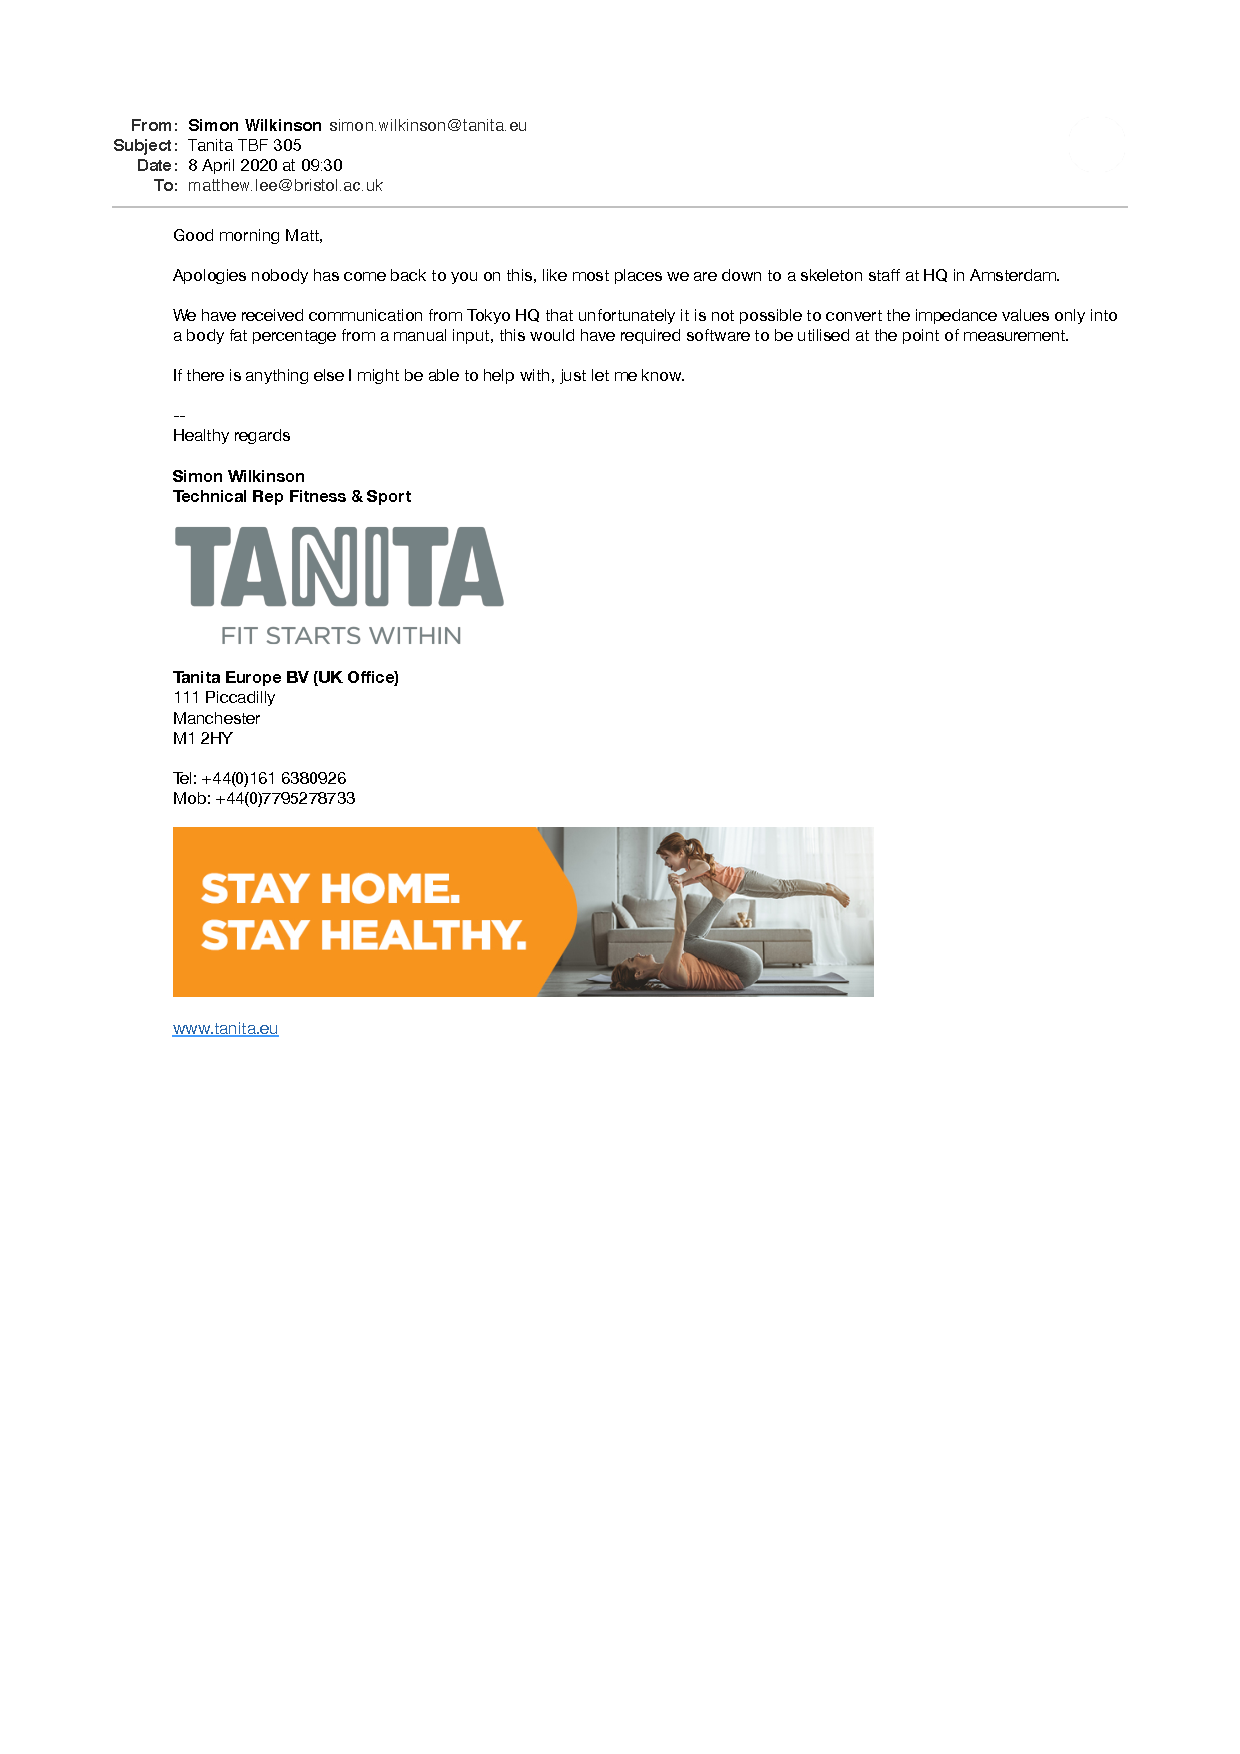
\includegraphics[height=1\textheight]{data/chapter4/supplement/Tanita_communication} \caption{Email communication with Tanita RE calculation of body fat percentage from raw impedance}\label{fig:appendix-chapter4-communications-tanita}
\end{figure}
\hypertarget{figures}{%
\subsection{Figures}\label{figures}}

\hypertarget{chapter4-appendix-figures-forestplots}{%
\subsubsection{Forestplots}\label{chapter4-appendix-figures-forestplots}}

\blandscape
\begin{figure}
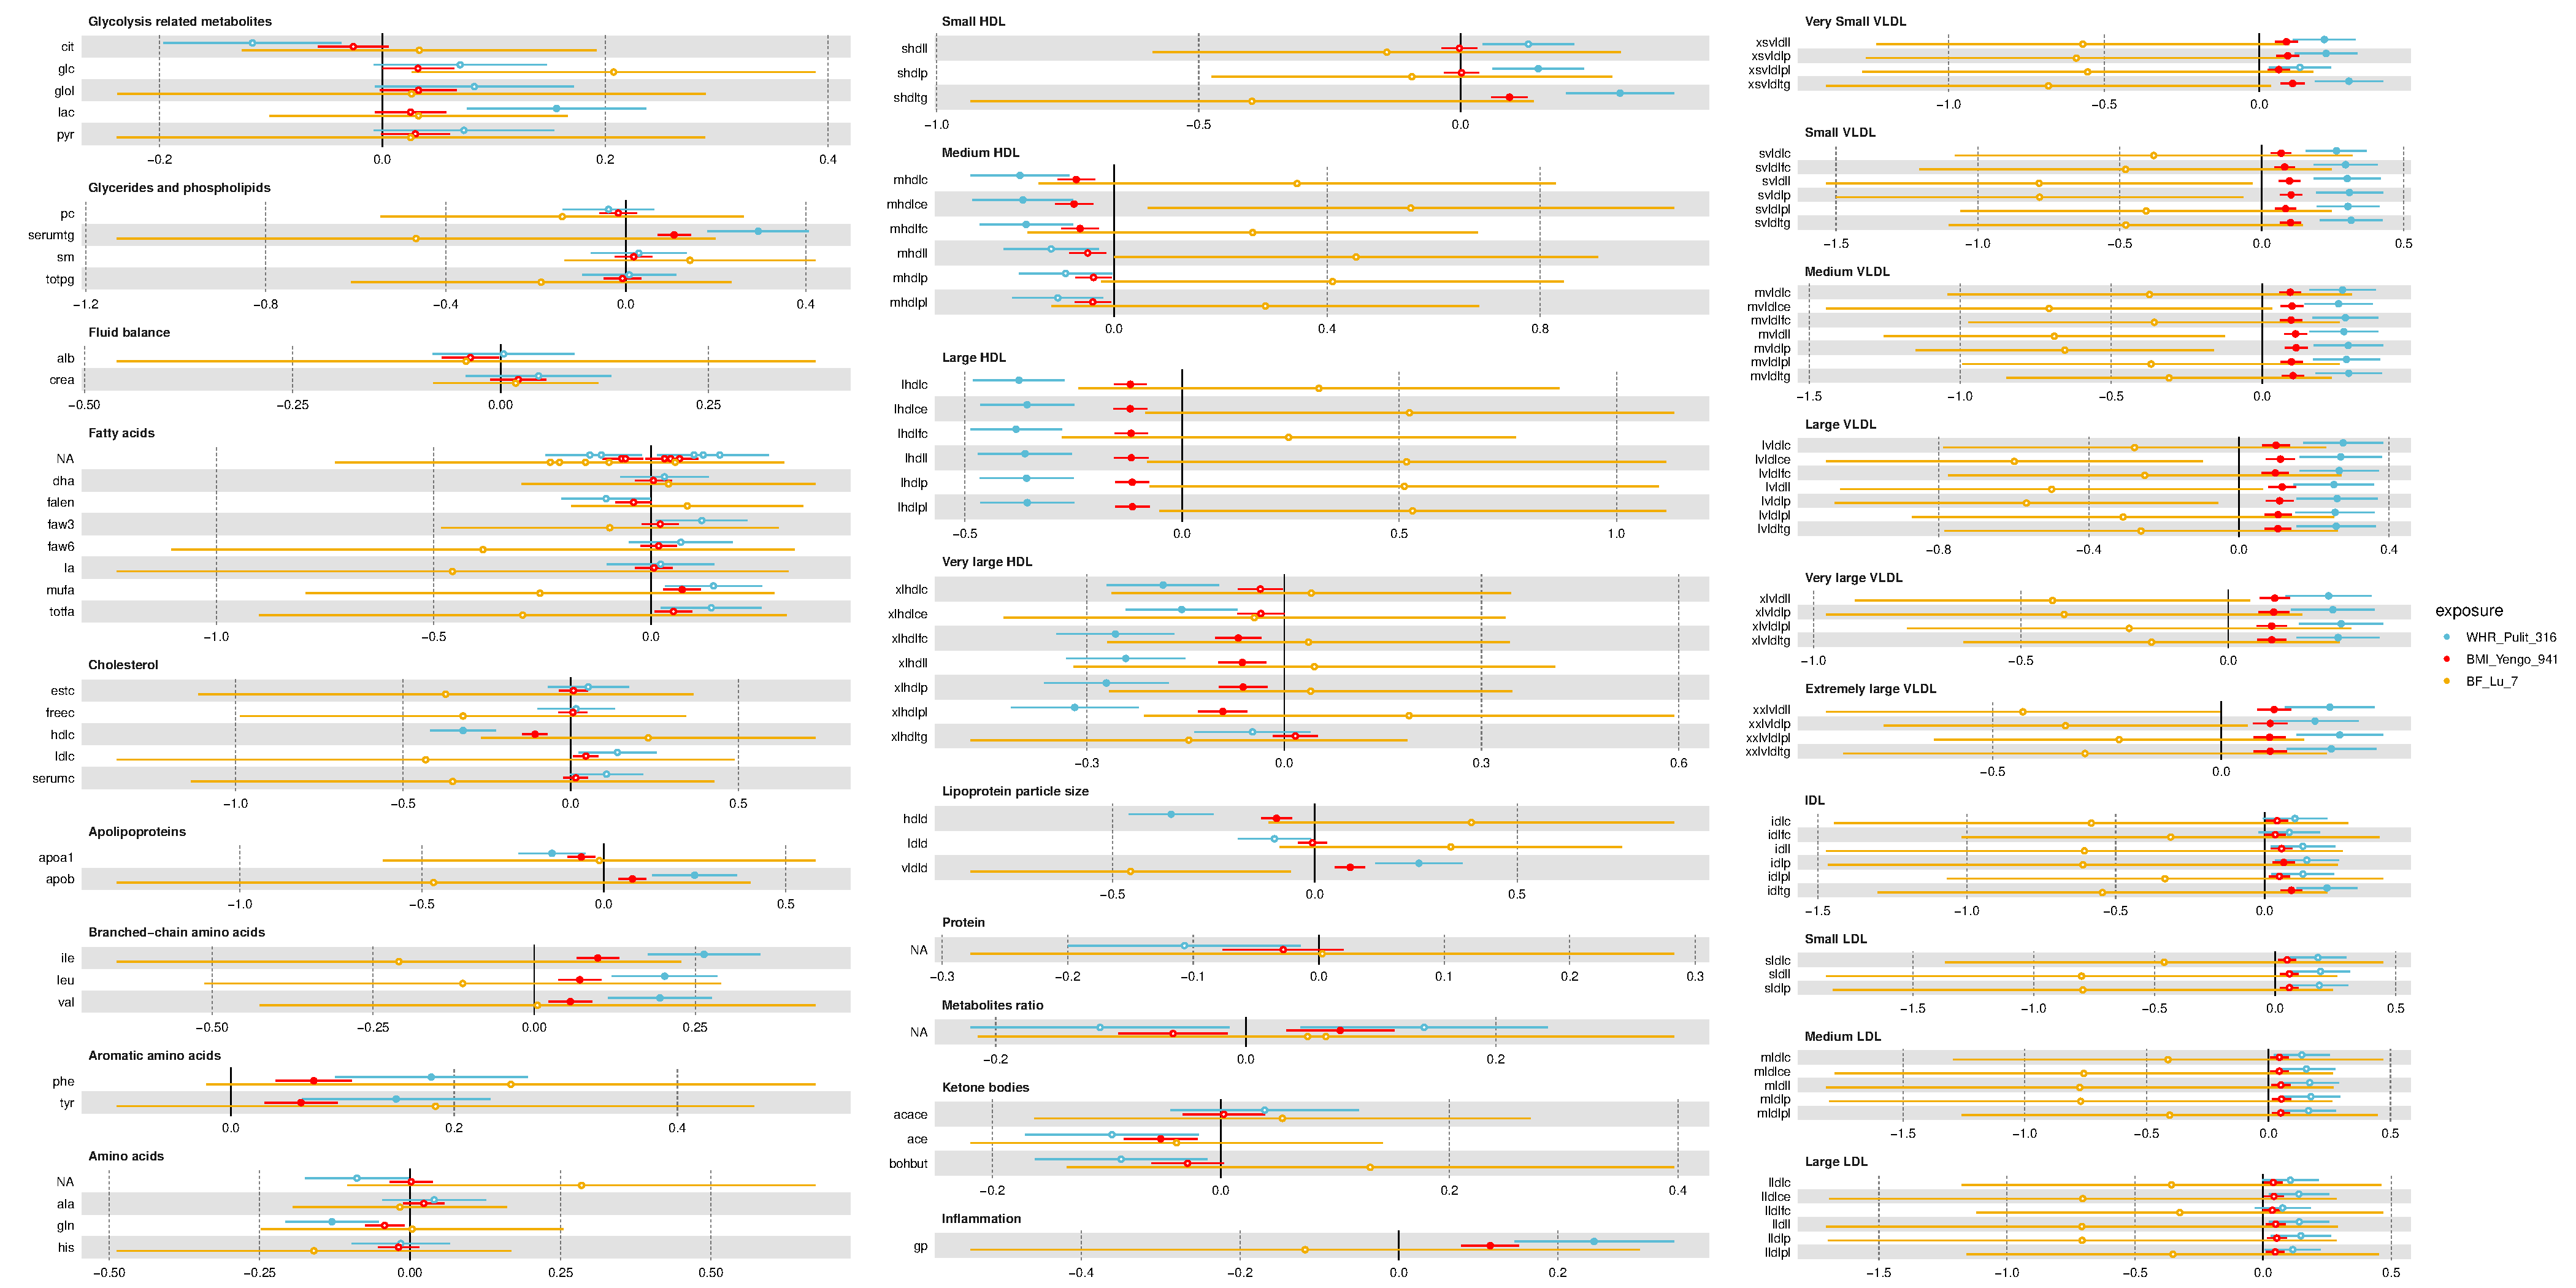
\includegraphics[width=1\linewidth]{data/chapter4/Supplement/forestplot_main} \caption{Forestplot of effect estimates from a linear regression}\label{fig:chapter4-appendix-figure-forestplot-main}
\end{figure}
\noindent 
\bsmall
\emph{Figure \ref{fig:chapter4-appendix-figure-forestplot-main} shows effect estimates and 95\% confidence intervals from model 2 for all exposures and age groups. Effect estimates are per-standard deviation increase in metabolite per-standard deviation increase in exposure.}
\esmall
\elandscape

\blandscape
\begin{figure}
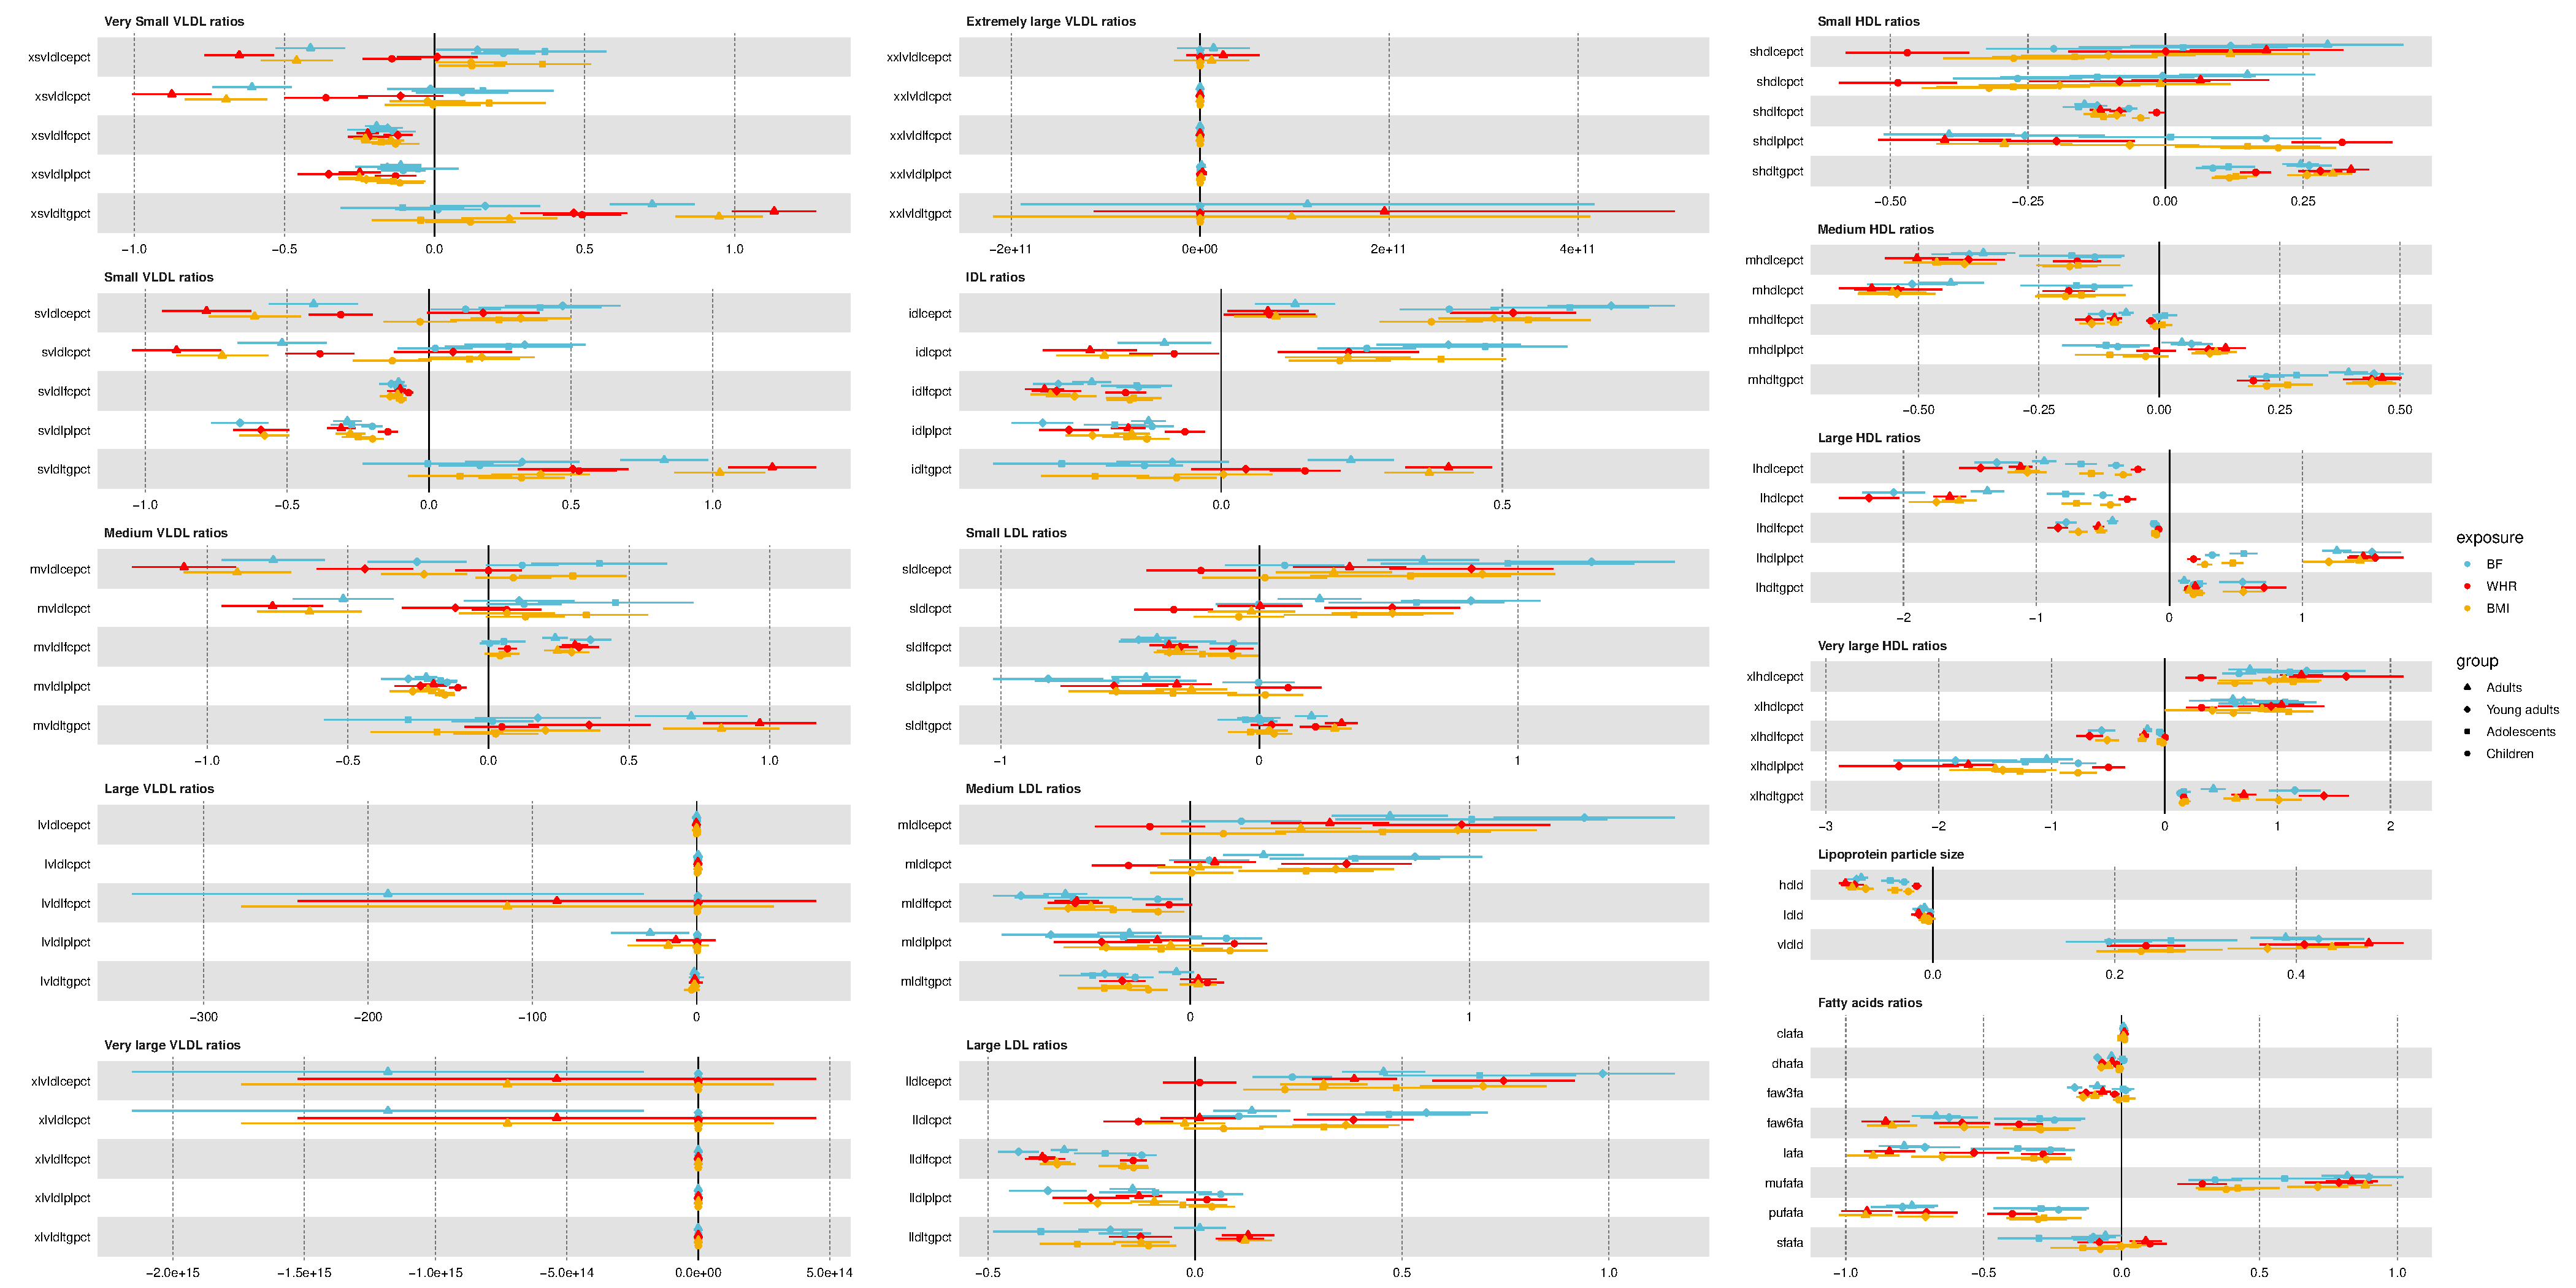
\includegraphics[width=1\linewidth]{data/chapter4/Supplement/forestplot_supplement} \caption{Forestplot of effect estimates from a linear regression, derived metabolites}\label{fig:chapter4-appendix-figure-forestplot-supplement}
\end{figure}
\noindent 
\bsmall
\emph{Figure \ref{fig:chapter4-appendix-figure-forestplot-supplement} shows effect estimates and 95\% confidence intervals from model 2 for all exposures and age groups. Effect estimates are per-standard deviation increase in metabolite per-standard deviation increase in exposure.}
\esmall
\elandscape

Forestplots show the effect estimate and 95\% confidence interval with multiple testing thresholds (solid points) set as the number of independent metabolites for each age group.

\hypertarget{circos-plots}{%
\subsubsection{Circos plots}\label{circos-plots}}

Circos plots show effect estimates and 95\% confidence intervals with multiple testing thresholds (solid points) set as the number of independent metabolites for each age group (set as the lowest number of independent metabolites for combined age group plots).

\hypertarget{chapter4-appendix-circosplot-supplement2}{%
\paragraph{Comparison of metabolic profile across exposures for each age group}\label{chapter4-appendix-circosplot-supplement2}}
\begin{figure}
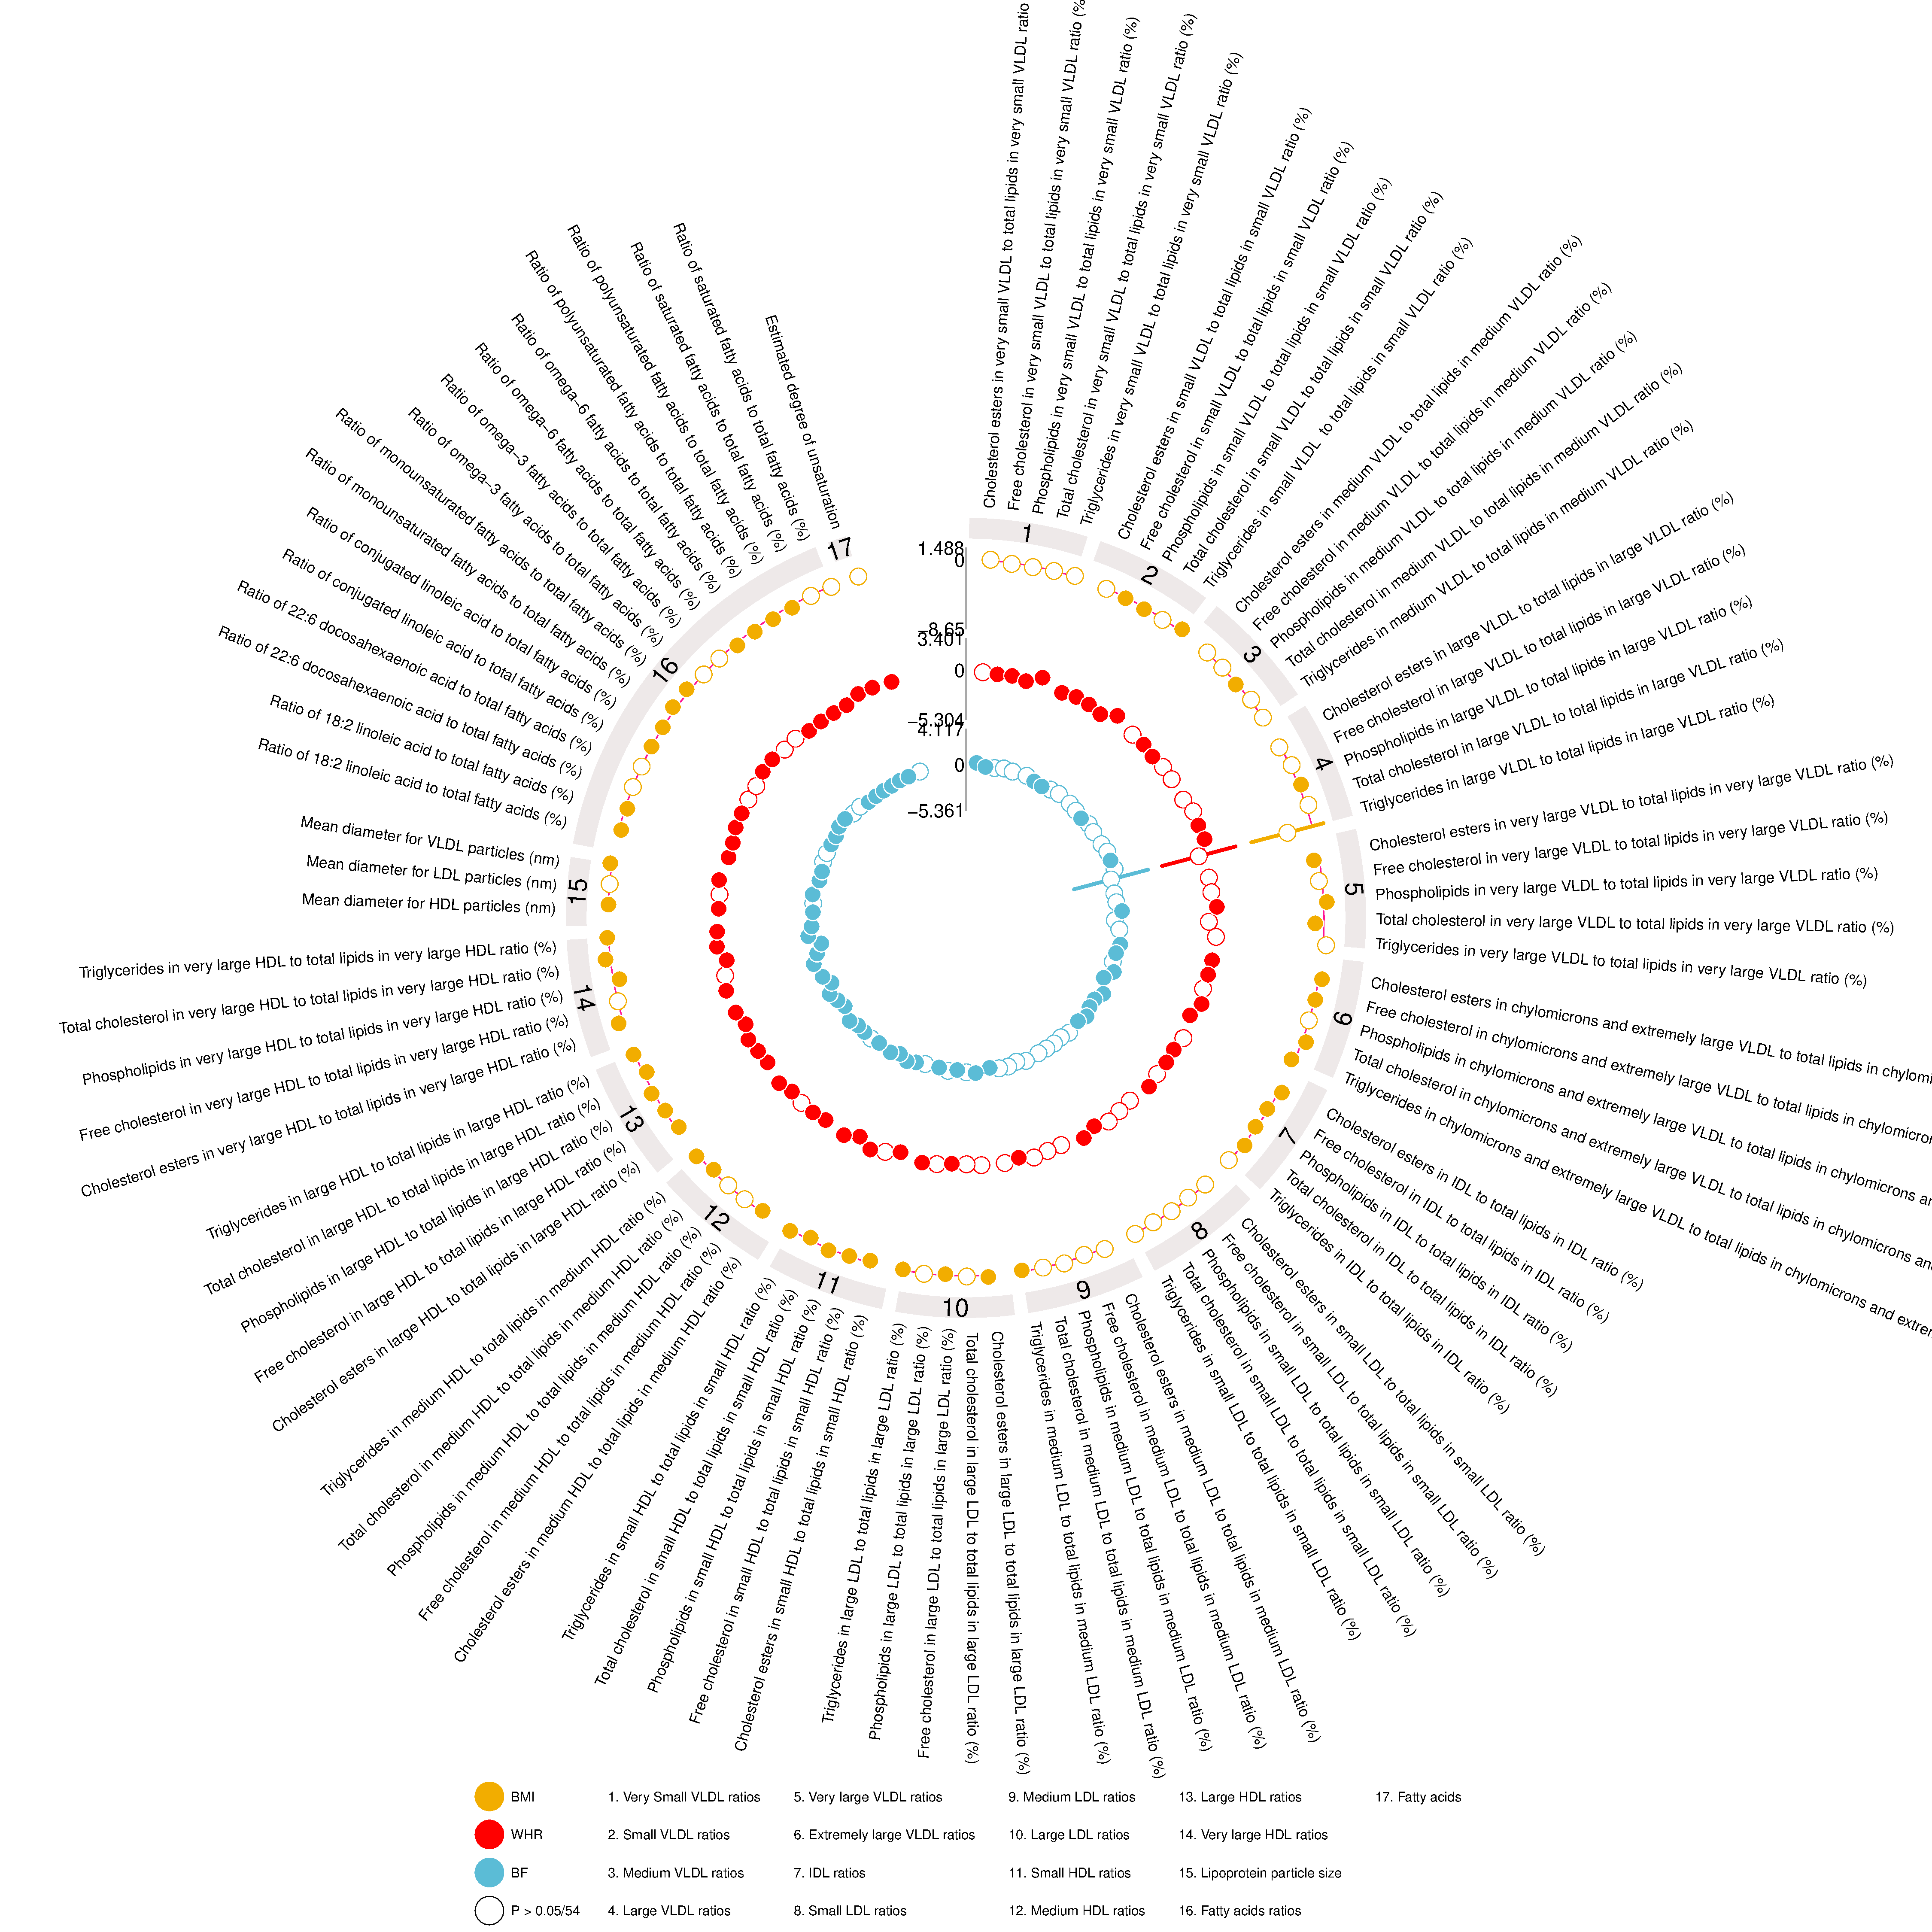
\includegraphics[width=1\linewidth]{data/chapter4/figures/circosplot_supplement_children} \caption{Circos plot of effect estimates from a linear regression in ALSPAC children, supplementary metabolites}\label{fig:plot-circos-supplement-children}
\end{figure}
\noindent 
\bsmall
\emph{Figure \ref{fig:plot-circos-supplement-children} shows effect estiamtes and 95\% confidence intervals from a linear regression. Each point represents a single result, with the metabolites labelled around the outside and each track representing an exposure; the outer track is BMI, the middle track is WHR, the inner track is BF. Solid points indicate a multiple testing threshold has been reached. BMI = body mass index; WHR = waist hip ratio; FFM = fat free mass.}
\esmall

\newpage
\begin{figure}
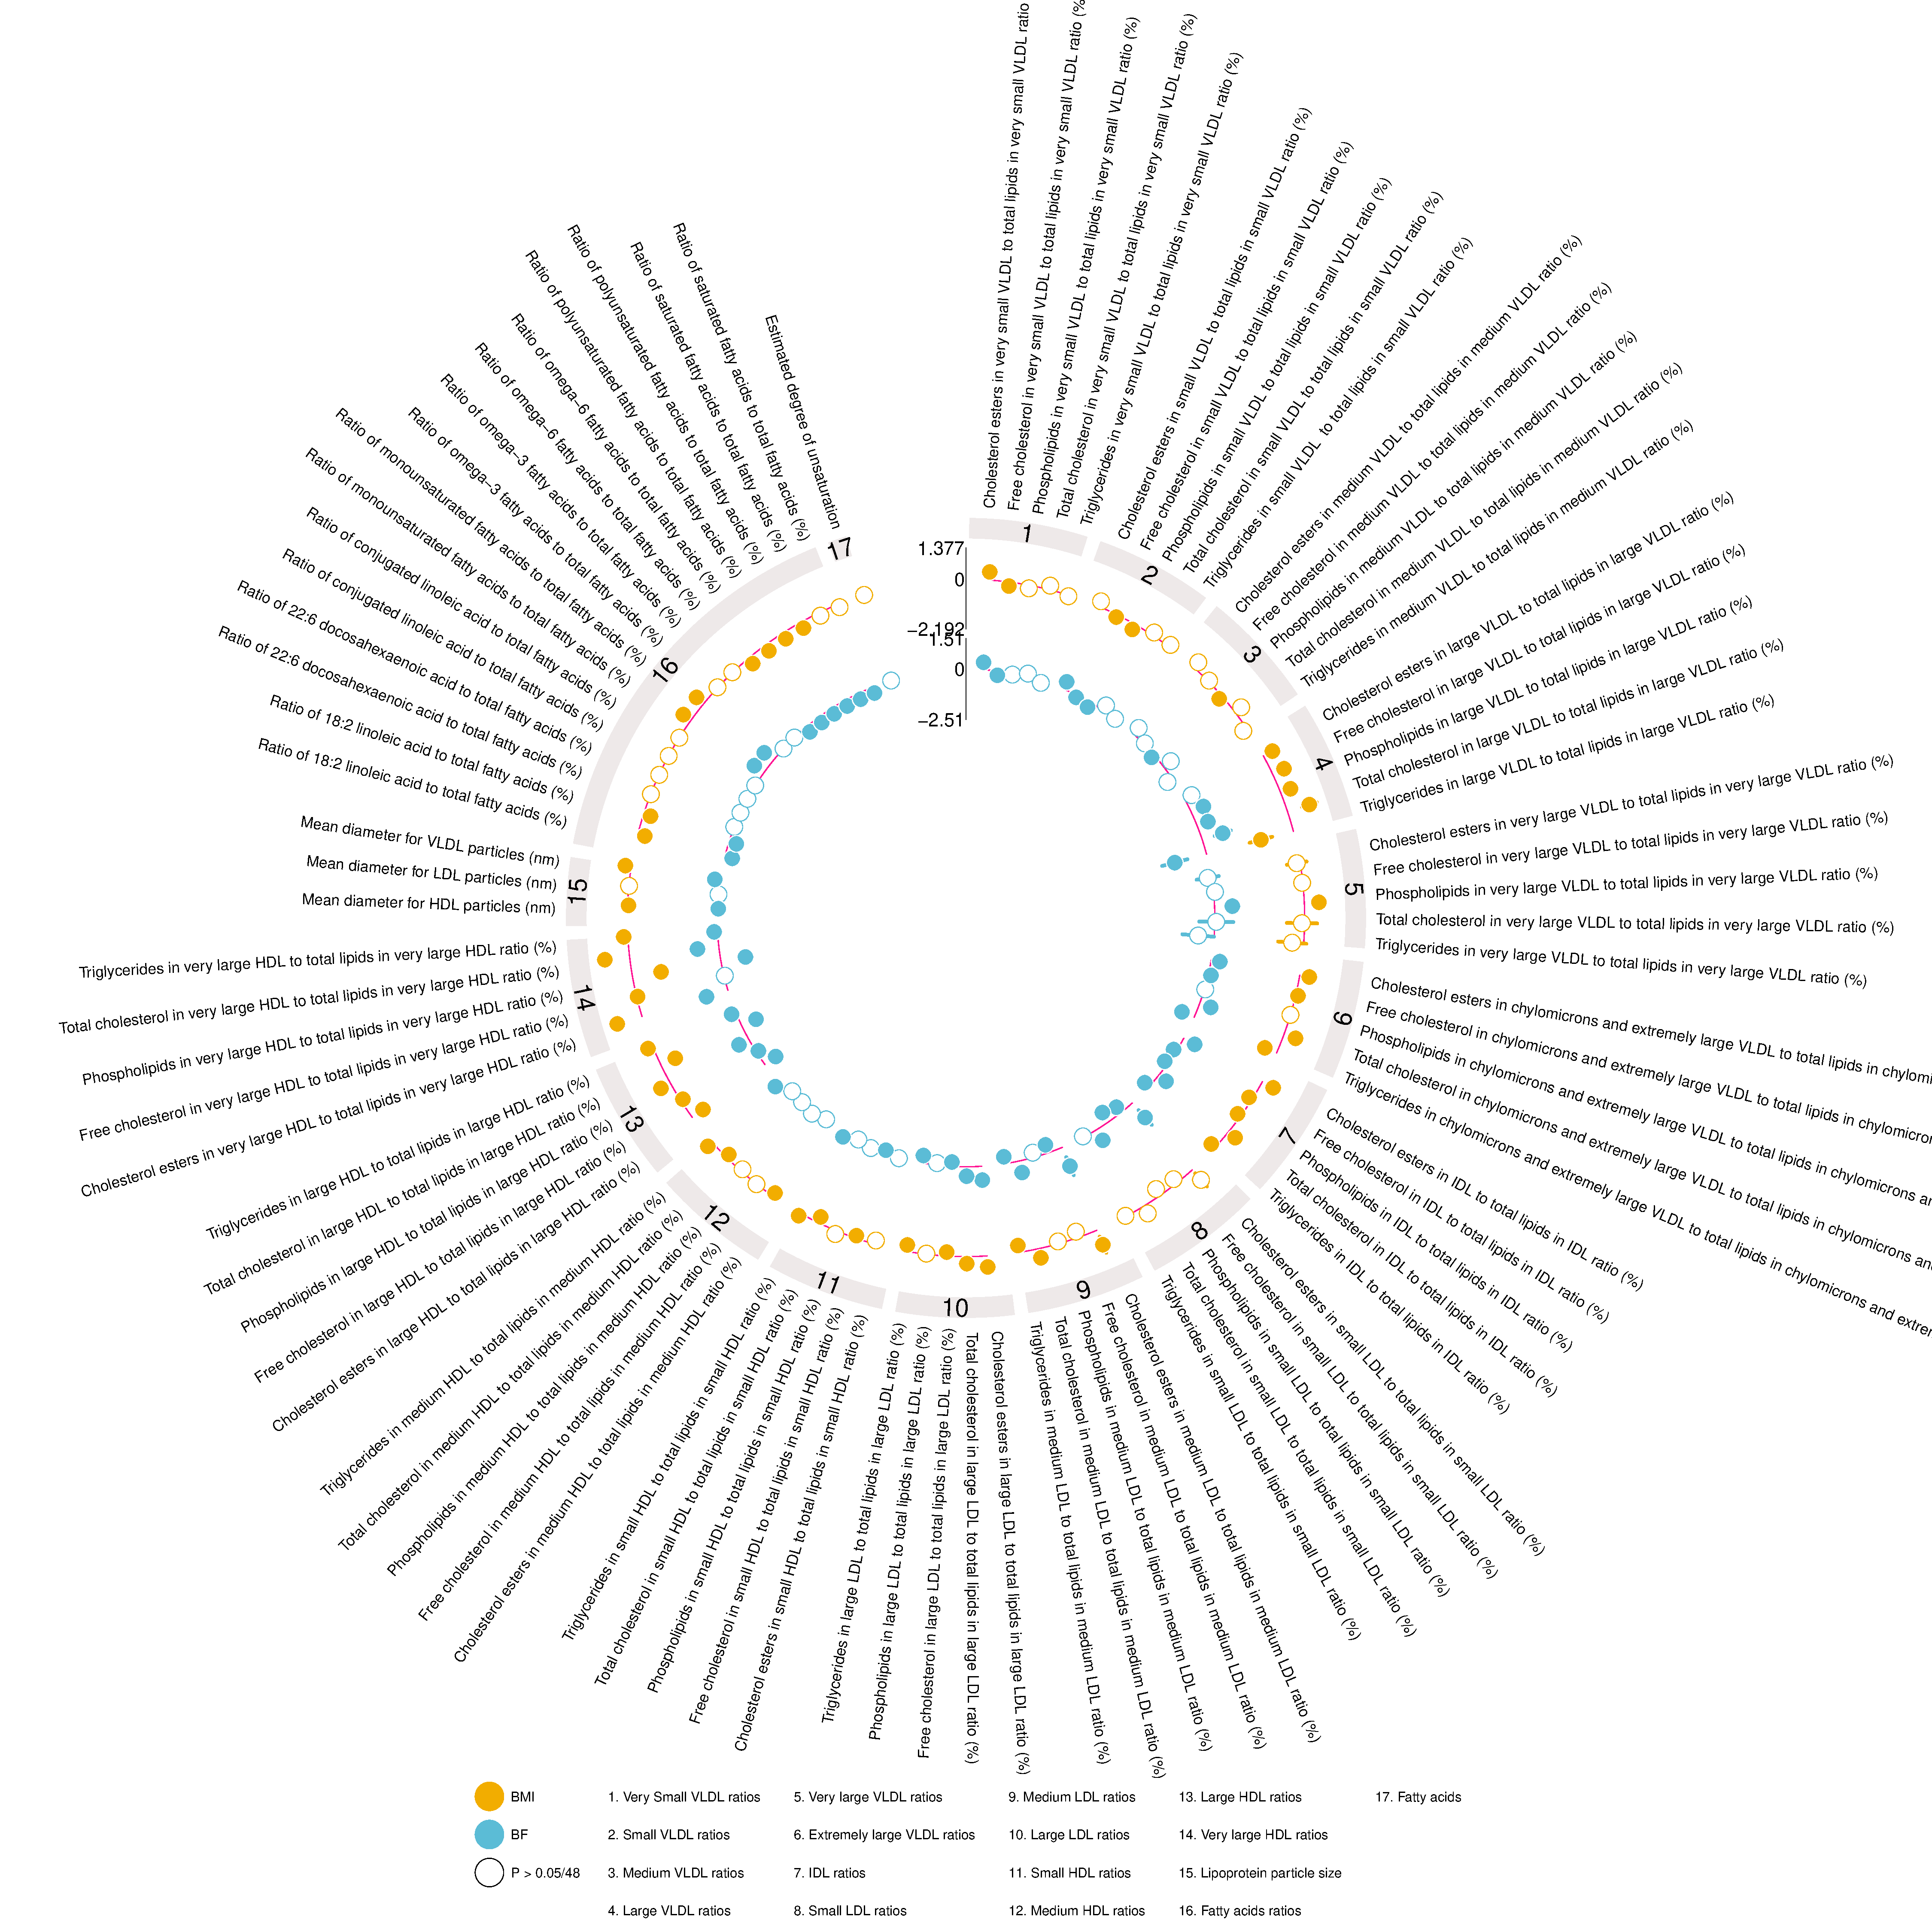
\includegraphics[width=1\linewidth]{data/chapter4/figures/circosplot_supplement_adolescents} \caption{Circos plot of effect estimates from a linear regression in ALSPAC adolescents, supplementary metabolites}\label{fig:plot-circos-supplement-adolescents}
\end{figure}
\noindent 
\bsmall
\emph{Figure \ref{fig:plot-circos-supplement-adolescents} shows effect estiamtes and 95\% confidence intervals from a linear regression. Each point represents a single result, with the metabolites labelled around the outside and each track representing an exposure; the outer track is BMI, the middle track is BF. Solid points indicate a multiple testing threshold has been reached. BMI = body mass index; BF = body fat percentage.}
\esmall

\newpage
\begin{figure}
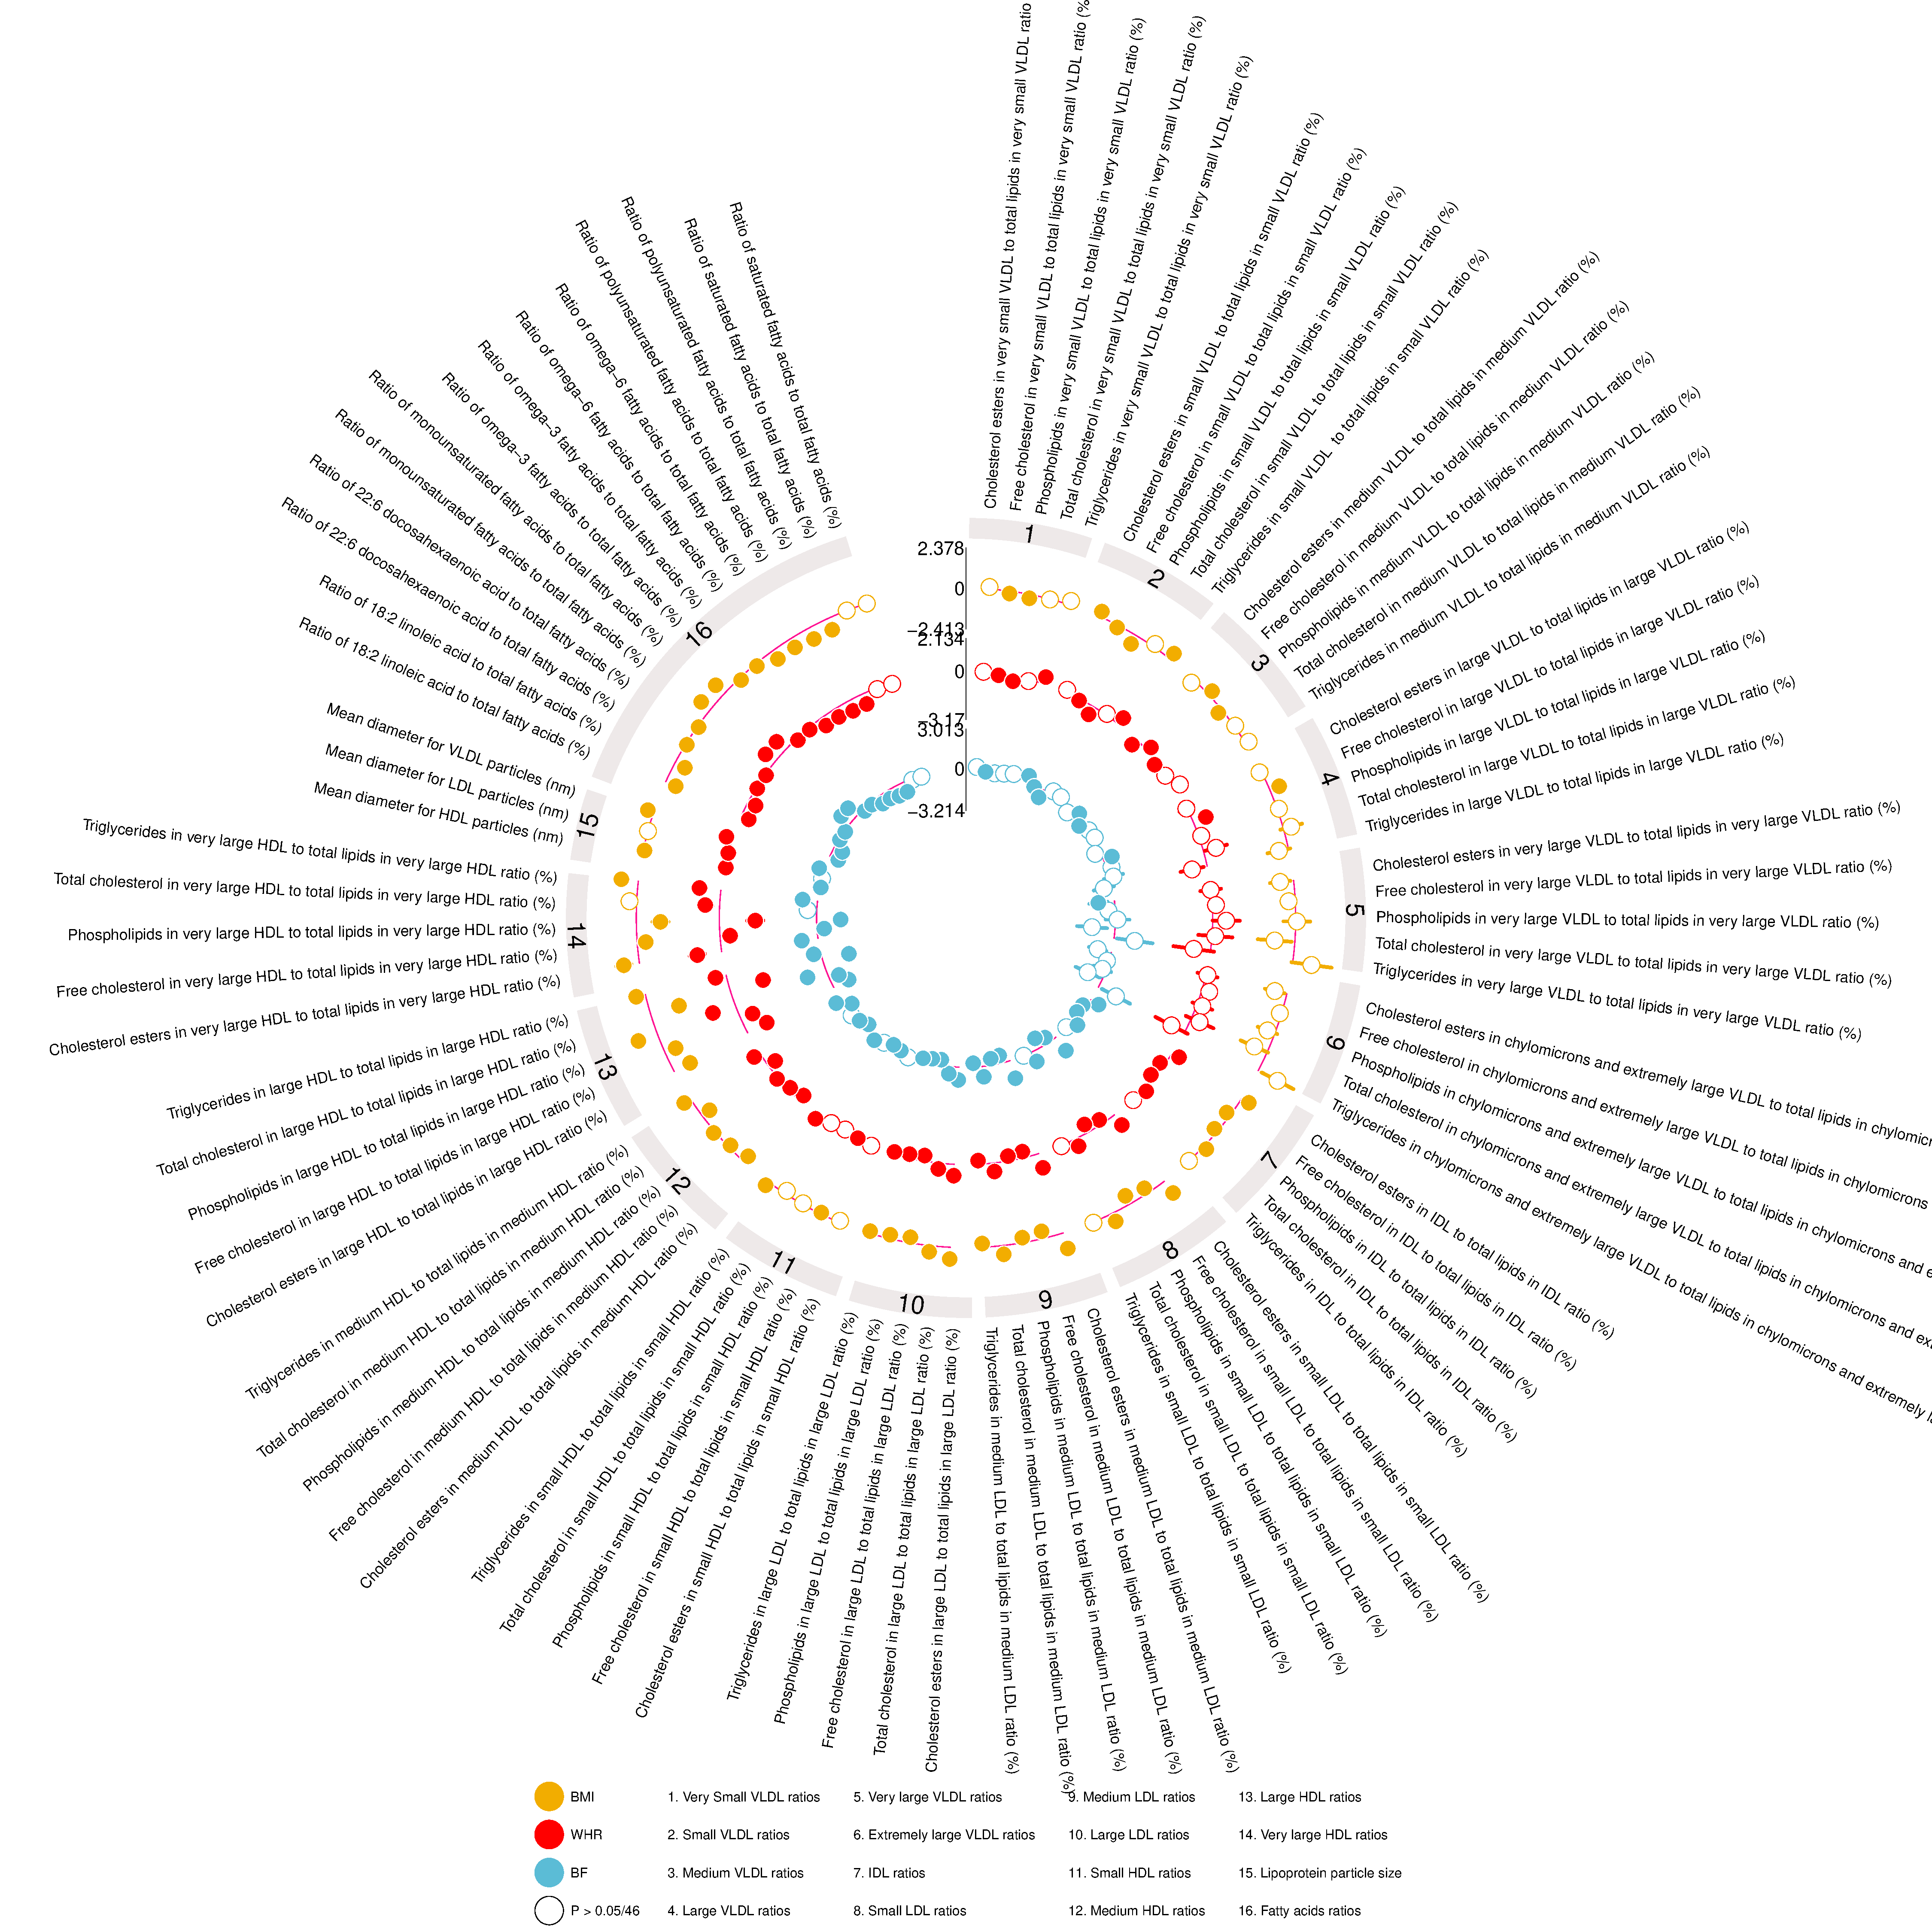
\includegraphics[width=1\linewidth]{data/chapter4/figures/circosplot_supplement_young_adults} \caption{Circos plot of effect estimates from a linear regression in ALSPAC young adults, supplementary metabolites}\label{fig:plot-circos-supplement-young-adults}
\end{figure}
\noindent 
\bsmall
\emph{Figure \ref{fig:plot-circos-supplement-young-adults} shows effect estiamtes and 95\% confidence intervals from a linear regression. Each point represents a single result, with the metabolites labelled around the outside and each track representing an exposure; the outer track is BMI, the middle track is WHR, the inner track is BF. Solid points indicate a multiple testing threshold has been reached. BMI = body mass index; WHR = waist hip ratio; BF = body fat percentage.}
\esmall

\newpage
\begin{figure}
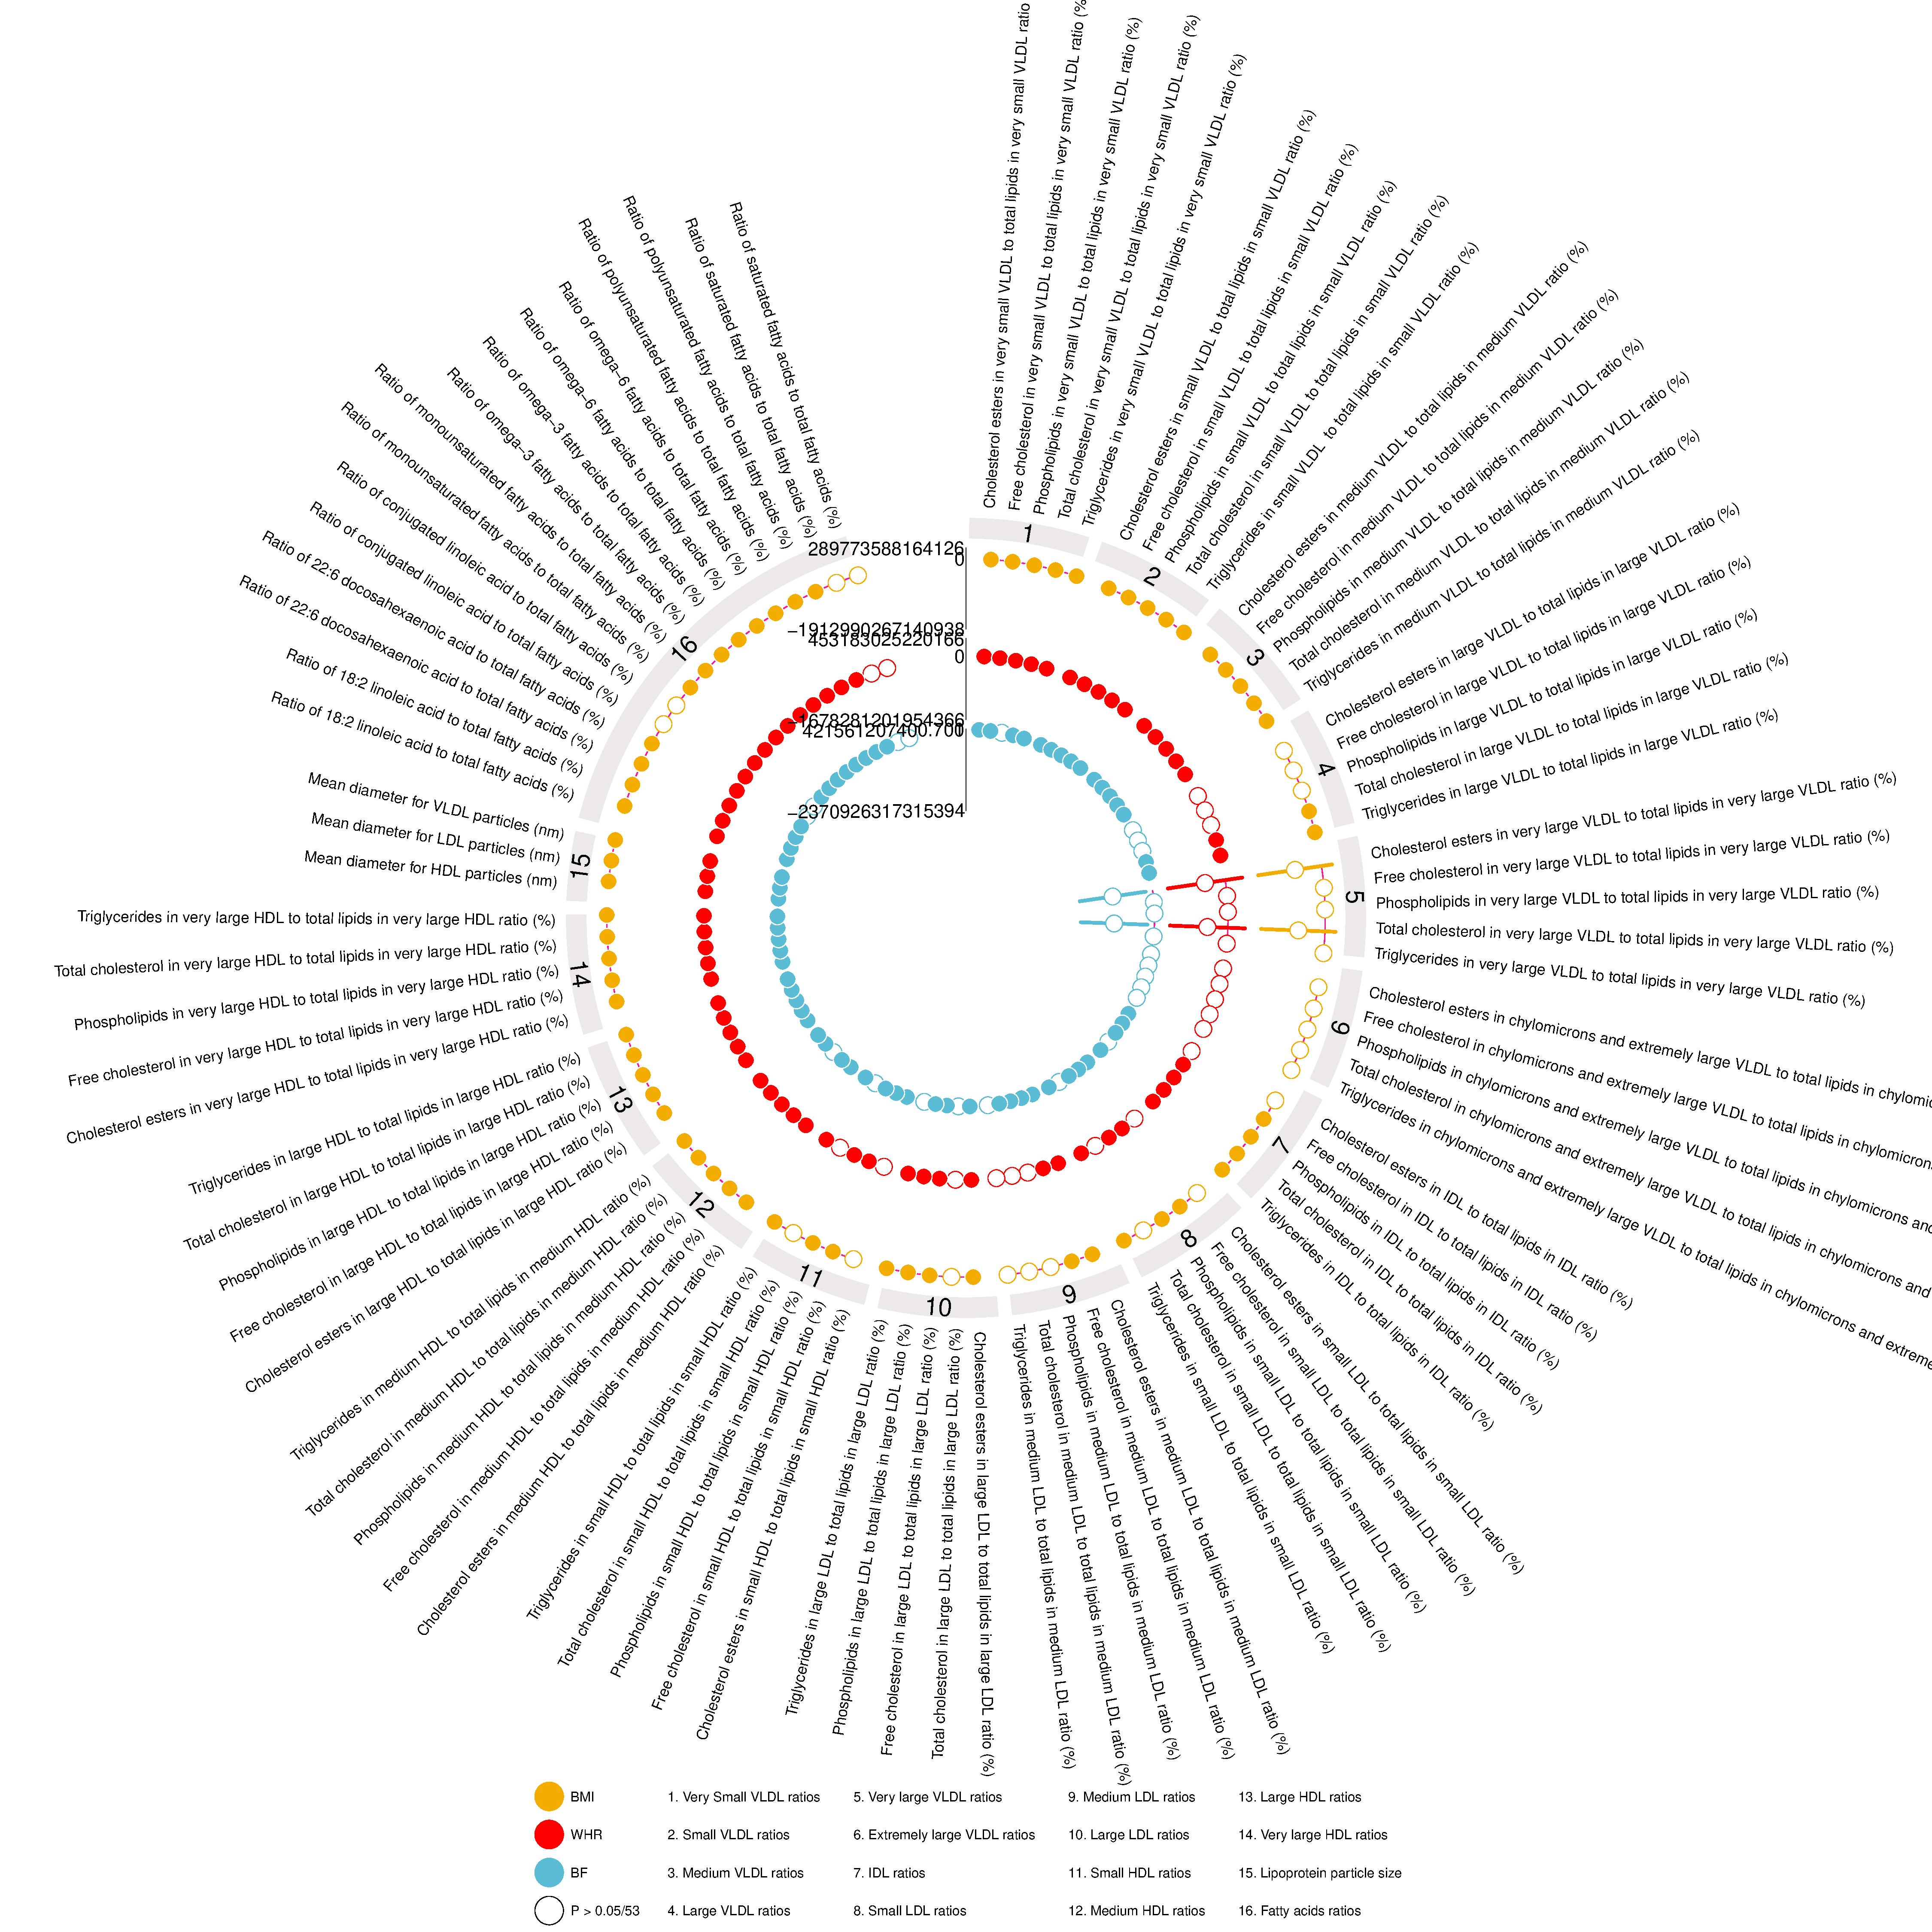
\includegraphics[width=1\linewidth]{data/chapter4/figures/circosplot_supplement_adults} \caption{Circos plot of effect estimates from a linear regression in ALSPAC adults, supplementary metabolites}\label{fig:plot-circos-supplement-adults}
\end{figure}
\noindent 
\bsmall
\emph{Figure \ref{fig:plot-circos-supplement-adults} shows effect estiamtes and 95\% confidence intervals from a linear regression. Each point represents a single result, with the metabolites labelled around the outside and each track representing an exposure; the outer track is BMI, the middle track is WHR, the inner track is BF. Solid points indicate a multiple testing threshold has been reached. BMI = body mass index; WHR = waist hip ratio; BF = body fat percentage.}
\esmall

\hypertarget{chapter5-appendix}{%
\section{Chapter 5}\label{chapter5-appendix}}

\blandscape
\begin{longtabu} to \linewidth {>{\raggedright}X>{\raggedright}X>{\raggedright}X>{\raggedright}X}
\caption{\label{tab:appendix-chapter5-table-metabolites}Metabolites from Kettunen et al (2016) used as outcomes in MR analysis}\\
\toprule
Abbreviation & Label & Class & subclass\\
\midrule
ala & Alanine (mmol/l) & Amino acids & Amino acids\\
gln & Glutamine (mmol/l) & Amino acids & Amino acids\\
his & Histidine (mmol/l) & Amino acids & Amino acids\\
ile & Isoleucine (mmol/l) & Amino acids & Branched-chain amino acids\\
leu & Leucine (mmol/l) & Amino acids & Branched-chain amino acids\\
\addlinespace
phe & Phenylalanine (mmol/l) & Amino acids & Aromatic amino acids\\
tyr & Tyrosine (mmol/l) & Amino acids & Aromatic amino acids\\
val & Valine (mmol/l) & Amino acids & Branched-chain amino acids\\
 & Urea & Amino acids & Amino acids\\
apoa1 & Apolipoprotein A-I (g/l) & Apolipoproteins & Apolipoproteins\\
\addlinespace
apob & Apolipoprotein B (g/l) & Apolipoproteins & Apolipoproteins\\
estc & Esterified cholesterol (mmol/l) & Cholesterol & Cholesterol\\
freec & Free cholesterol (mmol/l) & Cholesterol & Cholesterol\\
hdlc & Total cholesterol in HDL (mmol/l) & Cholesterol & Cholesterol\\
ldlc & Total cholesterol in LDL (mmol/l) & Cholesterol & Cholesterol\\
\addlinespace
serumc & Serum total cholesterol (mmol/l) & Cholesterol & Cholesterol\\
dha & 22:6, docosahexaenoic acid (mmol/l) & Fatty acids & Fatty acids\\
falen & Estimated description of fatty acid chain length, not actual carbon number & Fatty acids & Fatty acids\\
faw3 & Omega-3 fatty acids (mmol/l) & Fatty acids & Fatty acids\\
faw6 & Omega-6 fatty acids (mmol/l) & Fatty acids & Fatty acids\\
\addlinespace
la & 18:2, linoleic acid (mmol/l) & Fatty acids & Fatty acids\\
mufa & Monounsaturated fatty acids; 16:1, 18:1 (mmol/l) & Fatty acids & Fatty acids\\
totfa & Total fatty acids (mmol/l) & Fatty acids & Fatty acids\\
 & Average number of double bonds in a fatty acid chain & Fatty acids & Fatty acids\\
 & Average number of methylene groups in a fatty acid chain & Fatty acids & Fatty acids\\
\addlinespace
 & Omega-7, omega-9 and saturated fatty acids & Fatty acids & Fatty acids\\
 & Other polyunsaturated fatty acids than 18:2 & Fatty acids & Fatty acids\\
 & Ratio of bisallylic groups to total fatty acids & Fatty acids & Fatty acids\\
alb & Albumin (signal area) & Fluid balance & Fluid balance\\
crea & Creatinine (mmol/l) & Fluid balance & Fluid balance\\
\addlinespace
pc & Phosphatidylcholine and other cholines (mmol/l) & Glycerides and phospholipids & Glycerides and phospholipids\\
serumtg & Serum total triglycerides (mmol/l) & Glycerides and phospholipids & Glycerides and phospholipids\\
sm & Sphingomyelins (mmol/l) & Glycerides and phospholipids & Glycerides and phospholipids\\
totpg & Total phosphoglycerides (mmol/l) & Glycerides and phospholipids & Glycerides and phospholipids\\
cit & Citrate (mmol/l) & Glycolysis related metabolites & Glycolysis related metabolites\\
\addlinespace
glc & Glucose (mmol/l) & Glycolysis related metabolites & Glycolysis related metabolites\\
glol & Glycerol (mmol/l) & Glycolysis related metabolites & Glycolysis related metabolites\\
lac & Lactate (mmol/l) & Glycolysis related metabolites & Glycolysis related metabolites\\
pyr & Pyruvate (mmol/l) & Glycolysis related metabolites & Glycolysis related metabolites\\
gp & Glycoprotein acetyls, mainly a1-acid glycoprotein (mmol/l) & Inflammation & Inflammation\\
\addlinespace
acace & Acetoacetate (mmol/l) & Ketone bodies & Ketone bodies\\
ace & Acetate (mmol/l) & Ketone bodies & Ketone bodies\\
bohbut & 3-hydroxybutyrate (mmol/l) & Ketone bodies & Ketone bodies\\
hdld & Mean diameter for HDL particles (nm) & Lipoprotein particle size & Lipoprotein particle size\\
ldld & Mean diameter for LDL particles (nm) & Lipoprotein particle size & Lipoprotein particle size\\
\addlinespace
vldld & Mean diameter for VLDL particles (nm) & Lipoprotein particle size & Lipoprotein particle size\\
idlc & Total cholesterol in IDL (mmol/l) & Lipoprotein subclasses & IDL\\
idlfc & Free cholesterol in IDL (mmol/l) & Lipoprotein subclasses & IDL\\
idll & Total lipids in IDL (mmol/l) & Lipoprotein subclasses & IDL\\
idlp & Concentration of IDL particles (mol/l) & Lipoprotein subclasses & IDL\\
\addlinespace
idlpl & Phospholipids in IDL (mmol/l) & Lipoprotein subclasses & IDL\\
idltg & Triglycerides in IDL (mmol/l) & Lipoprotein subclasses & IDL\\
lhdlc & Total cholesterol in large HDL (mmol/l) & Lipoprotein subclasses & Large HDL\\
lhdlce & Cholesterol esters in large HDL (mmol/l) & Lipoprotein subclasses & Large HDL\\
lhdlfc & Free cholesterol in large HDL (mmol/l) & Lipoprotein subclasses & Large HDL\\
\addlinespace
lhdll & Total lipids in large HDL (mmol/l) & Lipoprotein subclasses & Large HDL\\
lhdlp & Concentration of large HDL particles (mol/l) & Lipoprotein subclasses & Large HDL\\
lhdlpl & Phospholipids in large HDL (mmol/l) & Lipoprotein subclasses & Large HDL\\
lldlc & Total cholesterol in large LDL (mmol/l) & Lipoprotein subclasses & Large LDL\\
lldlce & Cholesterol esters in large LDL (mmol/l) & Lipoprotein subclasses & Large LDL\\
\addlinespace
lldlfc & Free cholesterol in large LDL (mmol/l) & Lipoprotein subclasses & Large LDL\\
lldll & Total lipids in large LDL (mmol/l) & Lipoprotein subclasses & Large LDL\\
lldlp & Concentration of large LDL particles (mol/l) & Lipoprotein subclasses & Large LDL\\
lldlpl & Phospholipids in large LDL (mmol/l) & Lipoprotein subclasses & Large LDL\\
lvldlc & Total cholesterol in large VLDL (mmol/l) & Lipoprotein subclasses & Large VLDL\\
\addlinespace
lvldlce & Cholesterol esters in large VLDL (mmol/l) & Lipoprotein subclasses & Large VLDL\\
lvldlfc & Free cholesterol in large VLDL (mmol/l) & Lipoprotein subclasses & Large VLDL\\
lvldll & Total lipids in large VLDL (mmol/l) & Lipoprotein subclasses & Large VLDL\\
lvldlp & Concentration of large VLDL particles (mol/l) & Lipoprotein subclasses & Large VLDL\\
lvldlpl & Phospholipids in large VLDL (mmol/l) & Lipoprotein subclasses & Large VLDL\\
\addlinespace
lvldltg & Triglycerides in large VLDL (mmol/l) & Lipoprotein subclasses & Large VLDL\\
mhdlc & Total cholesterol in medium HDL (mmol/l) & Lipoprotein subclasses & Medium HDL\\
mhdlce & Cholesterol esters in medium HDL (mmol/l) & Lipoprotein subclasses & Medium HDL\\
mhdlfc & Free cholesterol in medium HDL (mmol/l) & Lipoprotein subclasses & Medium HDL\\
mhdll & Total lipids in medium HDL (mmol/l) & Lipoprotein subclasses & Medium HDL\\
\addlinespace
mhdlp & Concentration of medium HDL particles (mol/l) & Lipoprotein subclasses & Medium HDL\\
mhdlpl & Phospholipids in medium HDL (mmol/l) & Lipoprotein subclasses & Medium HDL\\
mldlc & Total cholesterol in medium LDL (mmol/l) & Lipoprotein subclasses & Medium LDL\\
mldlce & Cholesterol esters in medium LDL (mmol/l) & Lipoprotein subclasses & Medium LDL\\
mldll & Total lipids in medium LDL (mmol/l) & Lipoprotein subclasses & Medium LDL\\
\addlinespace
mldlp & Concentration of medium LDL particles (mol/l) & Lipoprotein subclasses & Medium LDL\\
mldlpl & Phospholipids in medium LDL (mmol/l) & Lipoprotein subclasses & Medium LDL\\
mvldlc & Total cholesterol in medium VLDL (mmol/l) & Lipoprotein subclasses & Medium VLDL\\
mvldlce & Cholesterol esters in medium VLDL (mmol/l) & Lipoprotein subclasses & Medium VLDL\\
mvldlfc & Free cholesterol in medium VLDL (mmol/l) & Lipoprotein subclasses & Medium VLDL\\
\addlinespace
mvldll & Total lipids in medium VLDL (mmol/l) & Lipoprotein subclasses & Medium VLDL\\
mvldlp & Concentration of medium VLDL particles (mol/l) & Lipoprotein subclasses & Medium VLDL\\
mvldlpl & Phospholipids in medium VLDL (mmol/l) & Lipoprotein subclasses & Medium VLDL\\
mvldltg & Triglycerides in medium VLDL (mmol/l) & Lipoprotein subclasses & Medium VLDL\\
shdll & Total lipids in small HDL (mmol/l) & Lipoprotein subclasses & Small HDL\\
\addlinespace
shdlp & Concentration of small HDL particles (mol/l) & Lipoprotein subclasses & Small HDL\\
shdltg & Triglycerides in small HDL (mmol/l) & Lipoprotein subclasses & Small HDL\\
sldlc & Total cholesterol in small LDL (mmol/l) & Lipoprotein subclasses & Small LDL\\
sldll & Total lipids in small LDL (mmol/l) & Lipoprotein subclasses & Small LDL\\
sldlp & Concentration of small LDL particles (mol/l) & Lipoprotein subclasses & Small LDL\\
\addlinespace
svldlc & Total cholesterol in small VLDL (mmol/l) & Lipoprotein subclasses & Small VLDL\\
svldlfc & Free cholesterol in small VLDL (mmol/l) & Lipoprotein subclasses & Small VLDL\\
svldll & Total lipids in small VLDL (mmol/l) & Lipoprotein subclasses & Small VLDL\\
svldlp & Concentration of small VLDL particles (mol/l) & Lipoprotein subclasses & Small VLDL\\
svldlpl & Phospholipids in small VLDL (mmol/l) & Lipoprotein subclasses & Small VLDL\\
\addlinespace
svldltg & Triglycerides in small VLDL (mmol/l) & Lipoprotein subclasses & Small VLDL\\
xlhdlc & Total cholesterol in very large HDL (mmol/l) & Lipoprotein subclasses & Very large HDL\\
xlhdlce & Cholesterol esters in very large HDL (mmol/l) & Lipoprotein subclasses & Very large HDL\\
xlhdlfc & Free cholesterol in very large HDL (mmol/l) & Lipoprotein subclasses & Very large HDL\\
xlhdll & Total lipids in very large HDL (mmol/l) & Lipoprotein subclasses & Very large HDL\\
\addlinespace
xlhdlp & Concentration of very large HDL particles (mol/l) & Lipoprotein subclasses & Very large HDL\\
xlhdlpl & Phospholipids in very large HDL (mmol/l) & Lipoprotein subclasses & Very large HDL\\
xlhdltg & Triglycerides in very large HDL (mmol/l) & Lipoprotein subclasses & Very large HDL\\
xlvldll & Total lipids in very large VLDL (mmol/l) & Lipoprotein subclasses & Very large VLDL\\
xlvldlp & Concentration of very large VLDL particles (mol/l) & Lipoprotein subclasses & Very large VLDL\\
\addlinespace
xlvldlpl & Phospholipids in very large VLDL (mmol/l) & Lipoprotein subclasses & Very large VLDL\\
xlvldltg & Triglycerides in very large VLDL (mmol/l) & Lipoprotein subclasses & Very large VLDL\\
xsvldll & Total lipids in very small VLDL (mmol/l) & Lipoprotein subclasses & Very Small VLDL\\
xsvldlp & Concentration of very small VLDL particles (mol/l) & Lipoprotein subclasses & Very Small VLDL\\
xsvldlpl & Phospholipids in very small VLDL (mmol/l) & Lipoprotein subclasses & Very Small VLDL\\
\addlinespace
xsvldltg & Triglycerides in very small VLDL (mmol/l) & Lipoprotein subclasses & Very Small VLDL\\
xxlvldll & Total lipids in chylomicrons and extremely large VLDL (mmol/l) & Lipoprotein subclasses & Extremely large VLDL\\
xxlvldlp & Concentration of chylomicrons and extremely large VLDL particles (mol/l) & Lipoprotein subclasses & Extremely large VLDL\\
xxlvldlpl & Phospholipids in chylomicrons and extremely large VLDL (mmol/l) & Lipoprotein subclasses & Extremely large VLDL\\
xxlvldltg & Triglycerides in chylomicrons and extremely large VLDL (mmol/l) & Lipoprotein subclasses & Extremely large VLDL\\
\addlinespace
 & Average number of methylene groups per double bond & Metabolites ratio & Metabolites ratio\\
 & Ratio of bisallylic groups to double bonds & Metabolites ratio & Metabolites ratio\\
 & Glycoproteins & Protein & Protein\\
\bottomrule
\end{longtabu}
\elandscape

\newpage
\blandscape
\begin{longtable}[t]{lrlllrrrlllll}
\caption{\label{tab:appendix-chapter5-table-exposures}Genetic instrumental variables}\\
\toprule
SNP & Chr & BP & EA & NEA & EAF & B & SE & P & Exp & Ref & Note & Clump\\
\midrule
rs41279738 & 1 & 110082551 & g & t & 0.025 & 0.388 & 0.065 & 2.72e-09 & BF & Hubel &  & No\\
rs11205303 & 1 & 149906413 & c & t & 0.398 & 0.137 & 0.021 & 6.77e-11 & BF & Hubel &  & No\\
rs543874 & 1 & 177889480 & g & a & 0.205 & 0.252 & 0.026 & 8.26e-23 & BF & Hubel &  & No\\
rs2644109 & 1 & 201797535 & c & t & 0.669 & -0.120 & 0.022 & 4.73e-08 & BF & Hubel &  & No\\
rs2820444 & 1 & 219741820 & g & a & 0.709 & -0.140 & 0.023 & 6.66e-10 & BF & Hubel &  & No\\
\addlinespace
rs12140153 & 1 & 62579891 & g & t & 0.909 & 0.214 & 0.036 & 3.35e-09 & BF & Hubel &  & No\\
rs11209948 & 1 & 72811904 & g & t & 0.394 & -0.116 & 0.021 & 3.59e-08 & BF & Hubel &  & No\\
rs71658797 & 1 & 77967507 & t & a & 0.884 & -0.179 & 0.032 & 2.17e-08 & BF & Hubel &  & Yes\\
rs159962 & 1 & 8490983 & c & t & 0.665 & -0.119 & 0.022 & 4.47e-08 & BF & Hubel &  & No\\
rs1128249 & 2 & 165528624 & g & t & 0.606 & -0.151 & 0.021 & 9.03e-13 & BF & Hubel &  & No\\
\addlinespace
rs10930502 & 2 & 172890588 & g & a & 0.302 & -0.134 & 0.023 & 2.81e-09 & BF & Hubel &  & Yes\\
rs7590658 & 2 & 205375133 & g & a & 0.078 & 0.251 & 0.040 & 4.12e-10 & BF & Hubel &  & No\\
rs2972138 & 2 & 227106217 & g & a & 0.654 & -0.120 & 0.022 & 2.7e-08 & BF & Hubel &  & No\\
rs59086897 & 2 & 25145173 & t & a & 0.506 & -0.193 & 0.021 & 1.33e-20 & BF & Hubel &  & No\\
rs13410783 & 2 & 36789166 & g & a & 0.365 & 0.127 & 0.022 & 3.14e-09 & BF & Hubel &  & No\\
\addlinespace
rs62104180 & 2 & 466003 & g & a & 0.952 & 0.350 & 0.047 & 1.17e-13 & BF & Hubel &  & No\\
rs6545714 & 2 & 59307725 & g & a & 0.394 & 0.144 & 0.021 & 1.09e-11 & BF & Hubel &  & No\\
rs4410328 & 2 & 69600683 & c & t & 0.589 & 0.117 & 0.021 & 2.58e-08 & BF & Hubel &  & No\\
rs11712037 & 3 & 12344730 & g & c & 0.116 & 0.270 & 0.032 & 2.44e-17 & BF & Hubel &  & No\\
rs1464419 & 3 & 153691260 & c & a & 0.328 & -0.122 & 0.022 & 2.89e-08 & BF & Hubel &  & No\\
\addlinespace
rs3749237 & 3 & 49770032 & g & a & 0.681 & -0.135 & 0.022 & 9.86e-10 & BF & Hubel &  & No\\
rs9818550 & 3 & 61271329 & g & t & 0.286 & -0.130 & 0.023 & 2.32e-08 & BF & Hubel &  & No\\
rs13107325 & 4 & 103188709 & c & t & 0.928 & -0.266 & 0.040 & 1.77e-11 & BF & Hubel &  & No\\
rs2192527 & 4 & 18329824 & g & a & 0.471 & 0.134 & 0.021 & 9.68e-11 & BF & Hubel &  & No\\
rs13130484 & 4 & 45175691 & c & t & 0.572 & -0.200 & 0.021 & 1.41e-21 & BF & Hubel &  & No\\
\addlinespace
rs6847975 & 4 & 80812960 & g & a & 0.650 & -0.137 & 0.022 & 2.55e-10 & BF & Hubel &  & No\\
rs2963469 & 5 & 158001309 & t & a & 0.357 & -0.140 & 0.022 & 1.7e-10 & BF & Hubel &  & No\\
rs13163173 & 5 & 87943620 & c & a & 0.834 & -0.186 & 0.028 & 5.72e-11 & BF & Hubel &  & No\\
rs1591805 & 6 & 126717064 & g & a & 0.501 & -0.120 & 0.021 & 8.21e-09 & BF & Hubel &  & No\\
rs62396185 & 6 & 26180634 & g & c & 0.739 & 0.184 & 0.024 & 6.3e-15 & BF & Hubel &  & No\\
\addlinespace
rs1046080 & 6 & 31595882 & c & a & 0.276 & -0.128 & 0.023 & 2.73e-08 & BF & Hubel &  & Yes\\
rs142550007 & 6 & 40267936 & g & a & 0.983 & -0.445 & 0.081 & 3.6e-08 & BF & Hubel &  & No\\
rs4711961 & 6 & 50833084 & g & a & 0.831 & -0.165 & 0.028 & 2.41e-09 & BF & Hubel &  & No\\
rs9320823 & 6 & 98429337 & c & t & 0.609 & 0.134 & 0.021 & 2.26e-10 & BF & Hubel &  & No\\
rs35682716 & 7 & 113021580 & c & t & 0.654 & 0.120 & 0.022 & 4.49e-08 & BF & Hubel &  & No\\
\addlinespace
rs972283 & 7 & 130466854 & g & a & 0.522 & -0.123 & 0.021 & 2.71e-09 & BF & Hubel &  & No\\
rs80206917 & 7 & 140159389 & c & t & 0.287 & -0.125 & 0.023 & 3.89e-08 & BF & Hubel &  & No\\
rs848457 & 7 & 77602503 & g & t & 0.383 & 0.121 & 0.021 & 1.21e-08 & BF & Hubel &  & No\\
rs7845090 & 8 & 73449940 & g & a & 0.297 & 0.142 & 0.023 & 6.72e-10 & BF & Hubel &  & No\\
rs4744546 & 9 & 136924744 & c & t & 0.558 & 0.123 & 0.021 & 3.85e-09 & BF & Hubel &  & No\\
\addlinespace
rs11515071 & 9 & 15855545 & c & t & 0.642 & 0.169 & 0.022 & 4.37e-15 & BF & Hubel &  & No\\
rs10968577 & 9 & 28415512 & c & t & 0.681 & -0.131 & 0.022 & 2.76e-09 & BF & Hubel &  & No\\
rs10749233 & 10 & 118777998 & g & c & 0.256 & 0.137 & 0.024 & 2.08e-08 & BF & Hubel &  & No\\
rs12253527 & 10 & 21819824 & g & a & 0.679 & -0.127 & 0.022 & 1.11e-08 & BF & Hubel &  & No\\
rs10999439 & 10 & 72386740 & c & t & 0.270 & 0.144 & 0.023 & 5.65e-10 & BF & Hubel &  & No\\
\addlinespace
rs2274224 & 10 & 96039597 & g & c & 0.562 & 0.168 & 0.021 & 7.93e-16 & BF & Hubel &  & No\\
rs11223600 & 11 & 133718882 & c & t & 0.906 & 0.203 & 0.035 & 1.05e-08 & BF & Hubel &  & No\\
rs61888762 & 11 & 27709630 & g & c & 0.316 & 0.155 & 0.022 & 2.66e-12 & BF & Hubel &  & No\\
rs10838137 & 11 & 43634973 & c & a & 0.666 & -0.135 & 0.022 & 9.59e-10 & BF & Hubel &  & No\\
rs59360790 & 11 & 47669175 & c & t & 0.400 & 0.176 & 0.021 & 6.31e-17 & BF & Hubel &  & No\\
\addlinespace
rs1426371 & 12 & 108629780 & g & a & 0.742 & 0.171 & 0.024 & 6.71e-13 & BF & Hubel &  & No\\
rs7133378 & 12 & 124409502 & g & a & 0.679 & -0.163 & 0.022 & 2.95e-13 & BF & Hubel &  & No\\
rs7975788 & 12 & 90273927 & g & t & 0.264 & 0.132 & 0.023 & 1.39e-08 & BF & Hubel &  & No\\
rs1928496 & 13 & 31012904 & c & t & 0.256 & -0.131 & 0.024 & 3.32e-08 & BF & Hubel &  & No\\
rs61969510 & 13 & 86484025 & c & t & 0.273 & 0.134 & 0.023 & 8.4e-09 & BF & Hubel &  & No\\
\addlinespace
rs7339274 & 13 & 99120272 & c & t & 0.715 & 0.144 & 0.023 & 2.06e-10 & BF & Hubel &  & No\\
rs8021531 & 14 & 75737909 & g & a & 0.711 & -0.127 & 0.023 & 2.85e-08 & BF & Hubel &  & No\\
rs55882426 & 14 & 94120712 & c & t & 0.498 & -0.116 & 0.021 & 2.54e-08 & BF & Hubel &  & No\\
rs3751585 & 15 & 51741056 & g & a & 0.803 & -0.143 & 0.026 & 3.11e-08 & BF & Hubel &  & No\\
rs28399271 & 15 & 67710011 & g & a & 0.735 & 0.155 & 0.024 & 4.58e-11 & BF & Hubel &  & No\\
\addlinespace
rs8031704 & 15 & 84651185 & c & a & 0.669 & -0.170 & 0.022 & 1.26e-14 & BF & Hubel &  & No\\
rs2411453 & 16 & 28632021 & g & t & 0.595 & -0.190 & 0.021 & 2.59e-19 & BF & Hubel &  & No\\
rs879620 & 16 & 4015729 & c & t & 0.402 & -0.135 & 0.021 & 2.03e-10 & BF & Hubel &  & No\\
rs1421085 & 16 & 53800954 & c & t & 0.394 & 0.319 & 0.021 & 1.03e-51 & BF & Hubel &  & No\\
rs11866219 & 16 & 69549749 & c & a & 0.576 & -0.137 & 0.021 & 1.34e-10 & BF & Hubel &  & No\\
\addlinespace
rs2941318 & 16 & 9312782 & g & a & 0.579 & 0.114 & 0.021 & 4.74e-08 & BF & Hubel &  & Yes\\
rs9893756 & 17 & 42321109 & c & t & 0.698 & -0.142 & 0.023 & 4.1e-10 & BF & Hubel &  & No\\
rs2080090 & 17 & 65828371 & t & a & 0.808 & -0.164 & 0.027 & 6.17e-10 & BF & Hubel &  & No\\
rs1834144 & 18 & 40744790 & c & a & 0.624 & 0.120 & 0.022 & 2.55e-08 & BF & Hubel &  & No\\
rs663640 & 18 & 57846077 & c & t & 0.778 & -0.176 & 0.025 & 2.1e-12 & BF & Hubel &  & No\\
\addlinespace
rs11666808 & 19 & 18383506 & c & t & 0.630 & -0.179 & 0.021 & 6.06e-17 & BF & Hubel &  & No\\
rs33823 & 19 & 34000725 & c & t & 0.360 & -0.142 & 0.022 & 8.41e-11 & BF & Hubel &  & No\\
rs1800437 & 19 & 46181392 & g & c & 0.808 & 0.151 & 0.026 & 6.91e-09 & BF & Hubel &  & No\\
rs1538482 & 20 & 47705496 & c & t & 0.308 & -0.139 & 0.022 & 6.3e-10 & BF & Hubel &  & No\\
rs7282639 & 21 & 46491155 & g & c & 0.322 & 0.121 & 0.022 & 4.81e-08 & BF & Hubel &  & No\\
\addlinespace
rs4821764 & 22 & 38599364 & g & a & 0.422 & 0.151 & 0.021 & 6.43e-13 & BF & Hubel &  & No\\
rs6728726 & 2 & 613976 & C & T & 0.840 & 0.037 & 0.007 & 2.9e-08 & BF & Lu &  & No\\
rs693839 & 13 & 79856289 & C & T & 0.310 & 0.030 & 0.005 & 9.3e-09 & BF & Lu &  & No\\
rs1558902 & 16 & 52361075 & A & T & 0.410 & 0.051 & 0.005 & 1.1e-25 & BF & Lu &  & No\\
rs9906944 & 17 & 44446419 & C & T & 0.660 & 0.035 & 0.006 & 1.9e-08 & BF & Lu &  & No\\
\addlinespace
rs6857 & 19 & 50084094 & C & T & 0.830 & 0.053 & 0.009 & 6.8e-10 & BF & Lu &  & No\\
rs6738627 & 2 & 165252696 & A & G & 0.370 & 0.030 & 0.005 & 1.8e-08 & BF & Lu & FA SNP & No\\
rs2943650 & 2 & 226814165 & C & T & 0.370 & 0.037 & 0.006 & 3.6e-10 & BF & Lu & FA SNP & No\\
rs17024393 & 1 & 109956211 & C & T & 0.040 & 0.066 & 0.009 & 7.03e-14 & BMI & Locke &  & No\\
rs543874 & 1 & 176156103 & G & A & 0.193 & 0.048 & 0.004 & 2.62e-35 & BMI & Locke &  & No\\
\addlinespace
rs2820292 & 1 & 200050910 & C & A & 0.555 & 0.020 & 0.003 & 1.83e-10 & BMI & Locke &  & No\\
rs657452 & 1 & 49362434 & A & G & 0.394 & 0.023 & 0.003 & 5.48e-13 & BMI & Locke &  & No\\
rs11583200 & 1 & 50332407 & C & T & 0.396 & 0.018 & 0.003 & 1.48e-08 & BMI & Locke &  & Yes\\
rs3101336 & 1 & 72523773 & C & T & 0.613 & 0.033 & 0.003 & 2.66e-26 & BMI & Locke &  & No\\
rs12566985 & 1 & 74774781 & G & A & 0.446 & 0.024 & 0.003 & 3.28e-15 & BMI & Locke &  & Yes\\
\addlinespace
rs12401738 & 1 & 78219349 & A & G & 0.352 & 0.021 & 0.003 & 1.15e-10 & BMI & Locke &  & No\\
rs11165643 & 1 & 96696685 & T & C & 0.583 & 0.022 & 0.003 & 2.07e-12 & BMI & Locke &  & No\\
rs2121279 & 2 & 142759755 & T & C & 0.152 & 0.025 & 0.004 & 2.31e-08 & BMI & Locke &  & No\\
rs1528435 & 2 & 181259207 & T & C & 0.631 & 0.018 & 0.003 & 1.2e-08 & BMI & Locke &  & No\\
rs7599312 & 2 & 213121476 & G & A & 0.724 & 0.022 & 0.003 & 1.17e-10 & BMI & Locke &  & No\\
\addlinespace
rs10182181 & 2 & 25003800 & G & A & 0.462 & 0.031 & 0.003 & 8.78e-24 & BMI & Locke &  & No\\
rs11126666 & 2 & 26782315 & A & G & 0.283 & 0.021 & 0.003 & 1.33e-09 & BMI & Locke &  & Yes\\
rs1016287 & 2 & 59159129 & T & C & 0.287 & 0.023 & 0.003 & 2.25e-11 & BMI & Locke &  & No\\
rs13021737 & 2 & 622348 & G & A & 0.828 & 0.060 & 0.004 & 1.11e-50 & BMI & Locke &  & No\\
rs11688816 & 2 & 62906552 & G & A & 0.525 & 0.017 & 0.003 & 1.89e-08 & BMI & Locke &  & Yes\\
\addlinespace
rs16851483 & 3 & 142758126 & T & G & 0.066 & 0.048 & 0.008 & 3.55e-10 & BMI & Locke &  & No\\
rs1516725 & 3 & 187306698 & C & T & 0.872 & 0.045 & 0.005 & 1.89e-22 & BMI & Locke &  & No\\
rs6804842 & 3 & 25081441 & G & A & 0.575 & 0.019 & 0.003 & 2.48e-09 & BMI & Locke &  & No\\
rs2365389 & 3 & 61211502 & C & T & 0.582 & 0.020 & 0.003 & 1.63e-10 & BMI & Locke &  & No\\
rs3849570 & 3 & 81874802 & A & C & 0.359 & 0.019 & 0.003 & 2.6e-08 & BMI & Locke &  & No\\
\addlinespace
rs13078960 & 3 & 85890280 & G & T & 0.196 & 0.030 & 0.004 & 1.74e-14 & BMI & Locke &  & No\\
rs13107325 & 4 & 103407732 & T & C & 0.072 & 0.048 & 0.007 & 1.83e-12 & BMI & Locke &  & No\\
rs11727676 & 4 & 145878514 & T & C & 0.910 & 0.036 & 0.006 & 2.55e-08 & BMI & Locke &  & No\\
rs10938397 & 4 & 44877284 & G & A & 0.434 & 0.040 & 0.003 & 3.21e-38 & BMI & Locke &  & No\\
rs17001654 & 4 & 77348592 & G & C & 0.153 & 0.031 & 0.005 & 7.76e-09 & BMI & Locke &  & No\\
\addlinespace
rs2112347 & 5 & 75050998 & T & G & 0.629 & 0.026 & 0.003 & 6.19e-17 & BMI & Locke &  & No\\
rs9400239 & 6 & 109084356 & C & T & 0.688 & 0.019 & 0.003 & 1.61e-08 & BMI & Locke &  & No\\
rs13191362 & 6 & 162953340 & A & G & 0.879 & 0.028 & 0.005 & 7.34e-09 & BMI & Locke &  & No\\
rs205262 & 6 & 34671142 & G & A & 0.273 & 0.022 & 0.004 & 1.75e-10 & BMI & Locke &  & No\\
rs2033529 & 6 & 40456631 & G & A & 0.293 & 0.019 & 0.003 & 1.39e-08 & BMI & Locke &  & Yes\\
\addlinespace
rs2207139 & 6 & 50953449 & G & A & 0.177 & 0.045 & 0.004 & 4.13e-29 & BMI & Locke &  & No\\
rs1167827 & 7 & 75001105 & G & A & 0.553 & 0.020 & 0.003 & 6.33e-10 & BMI & Locke &  & No\\
rs2245368 & 7 & 76446079 & C & T & 0.180 & 0.032 & 0.006 & 3.19e-08 & BMI & Locke &  & No\\
rs17405819 & 8 & 76969139 & T & C & 0.700 & 0.022 & 0.003 & 2.07e-11 & BMI & Locke &  & No\\
rs2033732 & 8 & 85242264 & C & T & 0.747 & 0.019 & 0.004 & 4.89e-08 & BMI & Locke &  & No\\
\addlinespace
rs6477694 & 9 & 110972163 & C & T & 0.365 & 0.017 & 0.003 & 2.67e-08 & BMI & Locke &  & No\\
rs1928295 & 9 & 119418304 & T & C & 0.548 & 0.019 & 0.003 & 7.91e-10 & BMI & Locke &  & No\\
rs10733682 & 9 & 128500735 & A & G & 0.478 & 0.017 & 0.003 & 1.83e-08 & BMI & Locke &  & No\\
rs4740619 & 9 & 15624326 & T & C & 0.542 & 0.018 & 0.003 & 4.56e-09 & BMI & Locke &  & No\\
rs10968576 & 9 & 28404339 & G & A & 0.320 & 0.025 & 0.003 & 6.61e-14 & BMI & Locke &  & No\\
\addlinespace
rs17094222 & 10 & 102385430 & C & T & 0.211 & 0.025 & 0.004 & 5.94e-11 & BMI & Locke &  & No\\
rs11191560 & 10 & 104859028 & C & T & 0.089 & 0.031 & 0.005 & 8.45e-09 & BMI & Locke &  & Yes\\
rs7903146 & 10 & 114748339 & C & T & 0.713 & 0.023 & 0.003 & 1.11e-11 & BMI & Locke &  & No\\
rs7899106 & 10 & 87400884 & G & A & 0.052 & 0.040 & 0.007 & 2.96e-08 & BMI & Locke &  & No\\
rs12286929 & 11 & 114527614 & G & A & 0.523 & 0.022 & 0.003 & 1.31e-12 & BMI & Locke &  & No\\
\addlinespace
rs11030104 & 11 & 27641093 & A & G & 0.792 & 0.041 & 0.004 & 5.56e-28 & BMI & Locke &  & No\\
rs2176598 & 11 & 43820854 & T & C & 0.251 & 0.020 & 0.004 & 2.97e-08 & BMI & Locke &  & No\\
rs3817334 & 11 & 47607569 & T & C & 0.407 & 0.026 & 0.003 & 5.15e-17 & BMI & Locke &  & No\\
rs4256980 & 11 & 8630515 & G & C & 0.646 & 0.021 & 0.003 & 2.9e-11 & BMI & Locke &  & No\\
rs11057405 & 12 & 121347850 & G & A & 0.901 & 0.031 & 0.006 & 2.02e-08 & BMI & Locke &  & No\\
\addlinespace
rs7138803 & 12 & 48533735 & A & G & 0.384 & 0.032 & 0.003 & 8.15e-24 & BMI & Locke &  & No\\
rs12016871 & 13 & 26915782 & T & C & 0.203 & 0.030 & 0.005 & 2.29e-10 & BMI & Locke &  & Yes\\
rs12429545 & 13 & 53000207 & A & G & 0.133 & 0.033 & 0.005 & 1.09e-12 & BMI & Locke &  & No\\
rs10132280 & 14 & 24998019 & C & A & 0.682 & 0.023 & 0.003 & 1.14e-11 & BMI & Locke &  & No\\
rs12885454 & 14 & 28806589 & C & A & 0.642 & 0.021 & 0.003 & 1.94e-10 & BMI & Locke &  & Yes\\
\addlinespace
rs11847697 & 14 & 29584863 & T & C & 0.042 & 0.049 & 0.008 & 3.99e-09 & BMI & Locke &  & Yes\\
rs7141420 & 14 & 78969207 & T & C & 0.527 & 0.024 & 0.003 & 1.23e-14 & BMI & Locke &  & No\\
rs3736485 & 15 & 49535902 & A & G & 0.454 & 0.018 & 0.003 & 7.41e-09 & BMI & Locke &  & No\\
rs16951275 & 15 & 65864222 & T & C & 0.784 & 0.031 & 0.004 & 1.91e-17 & BMI & Locke &  & No\\
rs12446632 & 16 & 19842890 & G & A & 0.865 & 0.040 & 0.005 & 1.48e-18 & BMI & Locke &  & No\\
\addlinespace
rs2650492 & 16 & 28240912 & A & G & 0.303 & 0.021 & 0.004 & 1.92e-09 & BMI & Locke &  & No\\
rs3888190 & 16 & 28796987 & A & C & 0.403 & 0.031 & 0.003 & 3.14e-23 & BMI & Locke &  & Yes\\
rs9925964 & 16 & 31037396 & A & G & 0.620 & 0.019 & 0.003 & 8.11e-10 & BMI & Locke &  & Yes\\
rs758747 & 16 & 3567359 & T & C & 0.265 & 0.023 & 0.004 & 7.47e-10 & BMI & Locke &  & No\\
rs1558902 & 16 & 52361075 & A & T & 0.415 & 0.082 & 0.003 & 7.51e-153 & BMI & Locke &  & No\\
\addlinespace
rs1000940 & 17 & 5223976 & G & A & 0.320 & 0.019 & 0.003 & 1.28e-08 & BMI & Locke &  & No\\
rs12940622 & 17 & 76230166 & G & A & 0.575 & 0.018 & 0.003 & 2.49e-09 & BMI & Locke &  & No\\
rs1808579 & 18 & 19358886 & C & T & 0.534 & 0.017 & 0.003 & 4.17e-08 & BMI & Locke &  & No\\
rs7243357 & 18 & 55034299 & T & G & 0.812 & 0.022 & 0.004 & 3.86e-08 & BMI & Locke &  & No\\
rs6567160 & 18 & 55980115 & C & T & 0.236 & 0.056 & 0.004 & 3.93e-53 & BMI & Locke &  & Yes\\
\addlinespace
rs17724992 & 19 & 18315825 & A & G & 0.746 & 0.019 & 0.004 & 3.42e-08 & BMI & Locke &  & No\\
rs29941 & 19 & 39001372 & G & A & 0.669 & 0.018 & 0.003 & 2.41e-08 & BMI & Locke &  & No\\
rs2075650 & 19 & 50087459 & A & G & 0.848 & 0.026 & 0.005 & 1.25e-08 & BMI & Locke &  & No\\
rs2287019 & 19 & 50894012 & C & T & 0.804 & 0.036 & 0.004 & 4.59e-18 & BMI & Locke &  & Yes\\
rs3810291 & 19 & 52260843 & A & G & 0.666 & 0.028 & 0.004 & 4.81e-15 & BMI & Locke &  & Yes\\
\addlinespace
rs1158103 & 1 & 101024370 & A & G & 0.556 & -0.010 & 0.002 & 6.73011e-09 & BMI & Yengo & COJO & Yes\\
rs1730859 & 1 & 107617707 & A & G & 0.658 & -0.011 & 0.002 & 6.37045e-11 & BMI & Yengo & COJO & No\\
rs12035149 & 1 & 107885018 & C & G & 0.777 & -0.016 & 0.002 & 7.39364e-14 & BMI & Yengo & COJO & Yes\\
rs17531363 & 1 & 107977075 & A & C & 0.697 & 0.013 & 0.002 & 1.81415e-10 & BMI & Yengo & COJO & Yes\\
rs7550711 & 1 & 110082886 & T & C & 0.031 & 0.064 & 0.005 & 2.38951e-35 & BMI & Yengo & COJO & No\\
\addlinespace
rs3768486 & 1 & 110123971 & A & G & 0.824 & -0.012 & 0.002 & 6.24605e-09 & BMI & Yengo & COJO & Yes\\
rs12033257 & 1 & 112318484 & A & G & 0.616 & 0.013 & 0.002 & 2.31124e-13 & BMI & Yengo & COJO & Yes\\
rs10779751 & 1 & 11284336 & A & G & 0.274 & 0.014 & 0.002 & 9.26946e-15 & BMI & Yengo & COJO & Yes\\
rs12731372 & 1 & 118852975 & T & C & 0.232 & 0.012 & 0.002 & 1.71405e-10 & BMI & Yengo & COJO & Yes\\
rs10923724 & 1 & 119546842 & T & C & 0.572 & -0.011 & 0.002 & 1.13784e-12 & BMI & Yengo & COJO & Yes\\
\addlinespace
rs6587552 & 1 & 151018861 & A & G & 0.241 & 0.015 & 0.002 & 6.46444e-13 & BMI & Yengo & COJO & No\\
rs905938 & 1 & 154991389 & T & C & 0.732 & -0.016 & 0.002 & 1.86277e-15 & BMI & Yengo & COJO & Yes\\
rs11577179 & 1 & 155983710 & A & G & 0.372 & -0.013 & 0.002 & 2.04004e-12 & BMI & Yengo & COJO & Yes\\
rs17448682 & 1 & 15966713 & T & C & 0.237 & 0.013 & 0.002 & 3.10028e-10 & BMI & Yengo & COJO & Yes\\
rs10733051 & 1 & 167280354 & A & G & 0.520 & 0.010 & 0.002 & 1.68951e-09 & BMI & Yengo & COJO & No\\
\addlinespace
rs696606 & 1 & 16828640 & A & G & 0.524 & 0.012 & 0.002 & 1.55353e-10 & BMI & Yengo & COJO & No\\
rs12044597 & 1 & 1708801 & A & G & 0.497 & -0.013 & 0.002 & 4.97046e-15 & BMI & Yengo & COJO & No\\
rs761423 & 1 & 17301672 & T & C & 0.550 & 0.012 & 0.002 & 6.90881e-13 & BMI & Yengo & COJO & No\\
rs912768 & 1 & 173473713 & C & G & 0.402 & 0.042 & 0.004 & 4.31118e-32 & BMI & Yengo & COJO & Yes\\
rs12039524 & 1 & 173549827 & A & G & 0.175 & -0.049 & 0.005 & 3.62648e-26 & BMI & Yengo & COJO & Yes\\
\addlinespace
rs11803119 & 1 & 174002465 & A & T & 0.018 & 0.059 & 0.009 & 7.67801e-11 & BMI & Yengo & COJO & No\\
rs6681627 & 1 & 174126742 & A & C & 0.152 & -0.057 & 0.005 & 1.69514e-27 & BMI & Yengo & COJO & Yes\\
rs12564992 & 1 & 174478100 & A & G & 0.886 & -0.038 & 0.004 & 4.51994e-26 & BMI & Yengo & COJO & Yes\\
rs6700816 & 1 & 174883994 & A & T & 0.968 & 0.033 & 0.005 & 2.4252e-10 & BMI & Yengo & COJO & No\\
rs11590474 & 1 & 174972588 & T & C & 0.792 & -0.036 & 0.004 & 8.69777e-23 & BMI & Yengo & COJO & Yes\\
\addlinespace
rs17302346 & 1 & 174983543 & T & C & 0.976 & -0.041 & 0.007 & 4.17082e-09 & BMI & Yengo & COJO & Yes\\
rs543874 & 1 & 177889480 & A & G & 0.805 & -0.047 & 0.002 & 2.86043e-116 & BMI & Yengo & COJO & Yes\\
rs10920678 & 1 & 190239907 & A & G & 0.429 & 0.016 & 0.002 & 1.35149e-19 & BMI & Yengo & COJO & No\\
rs12041258 & 1 & 195047936 & T & C & 0.771 & 0.015 & 0.002 & 1.78277e-12 & BMI & Yengo & COJO & No\\
rs3762396 & 1 & 19510394 & A & G & 0.385 & 0.011 & 0.002 & 8.56253e-09 & BMI & Yengo & COJO & Yes\\
\addlinespace
rs10754210 & 1 & 197012111 & A & G & 0.311 & -0.012 & 0.002 & 5.43686e-12 & BMI & Yengo & COJO & Yes\\
rs2820311 & 1 & 201841476 & A & G & 0.663 & -0.018 & 0.002 & 1.03187e-15 & BMI & Yengo & COJO & No\\
rs9077 & 1 & 202116238 & A & G & 0.330 & -0.016 & 0.002 & 2.79645e-14 & BMI & Yengo & COJO & Yes\\
rs823074 & 1 & 205774839 & T & C & 0.588 & 0.012 & 0.002 & 4.55219e-12 & BMI & Yengo & COJO & No\\
rs17014375 & 1 & 209543560 & T & G & 0.865 & -0.016 & 0.003 & 1.17921e-10 & BMI & Yengo & COJO & Yes\\
\addlinespace
rs11118308 & 1 & 219633869 & A & G & 0.530 & 0.010 & 0.002 & 3.34527e-10 & BMI & Yengo & COJO & No\\
rs10915840 & 1 & 225668524 & A & G & 0.283 & -0.013 & 0.002 & 1.07384e-10 & BMI & Yengo & COJO & No\\
rs967605 & 1 & 23399932 & T & C & 0.833 & -0.017 & 0.002 & 3.67663e-13 & BMI & Yengo & COJO & Yes\\
rs2491864 & 1 & 242986063 & A & G & 0.215 & 0.013 & 0.002 & 3.45974e-10 & BMI & Yengo & COJO & No\\
rs12042959 & 1 & 243533273 & A & G & 0.850 & 0.018 & 0.002 & 1.15518e-13 & BMI & Yengo & COJO & No\\
\addlinespace
rs3753549 & 1 & 243722892 & T & C & 0.856 & -0.023 & 0.003 & 6.93267e-19 & BMI & Yengo & COJO & Yes\\
rs7535528 & 1 & 2444414 & A & G & 0.374 & -0.015 & 0.002 & 6.52211e-16 & BMI & Yengo & COJO & No\\
rs785278 & 1 & 33307987 & A & T & 0.177 & -0.015 & 0.002 & 1.70527e-10 & BMI & Yengo & COJO & No\\
rs4653017 & 1 & 33776728 & T & C & 0.682 & 0.011 & 0.002 & 3.23466e-09 & BMI & Yengo & COJO & Yes\\
rs9426003 & 1 & 34602870 & A & G & 0.295 & -0.011 & 0.002 & 3.96435e-09 & BMI & Yengo & COJO & No\\
\addlinespace
rs11583122 & 1 & 38053458 & T & C & 0.079 & 0.017 & 0.003 & 9.13865e-09 & BMI & Yengo & COJO & Yes\\
rs2282231 & 1 & 39569571 & T & C & 0.225 & 0.013 & 0.002 & 3.81569e-10 & BMI & Yengo & COJO & Yes\\
rs346722 & 1 & 45620134 & T & C & 0.115 & 0.025 & 0.004 & 6.975e-11 & BMI & Yengo & COJO & No\\
rs946526 & 1 & 46487168 & T & C & 0.043 & -0.032 & 0.005 & 6.86037e-12 & BMI & Yengo & COJO & Yes\\
rs2275426 & 1 & 46487552 & A & G & 0.434 & 0.016 & 0.002 & 1.57379e-15 & BMI & Yengo & COJO & Yes\\
\addlinespace
rs6700838 & 1 & 47700027 & T & C & 0.596 & -0.019 & 0.002 & 1.65645e-25 & BMI & Yengo & COJO & Yes\\
rs7531656 & 1 & 49828663 & A & G & 0.325 & 0.019 & 0.002 & 2.39351e-28 & BMI & Yengo & COJO & No\\
rs2356865 & 1 & 50836334 & T & C & 0.295 & -0.012 & 0.002 & 6.45053e-10 & BMI & Yengo & COJO & Yes\\
rs2481665 & 1 & 62594677 & T & C & 0.559 & 0.015 & 0.002 & 4.15622e-20 & BMI & Yengo & COJO & No\\
rs11208662 & 1 & 65987164 & C & G & 0.088 & 0.021 & 0.003 & 1.14484e-11 & BMI & Yengo & COJO & Yes\\
\addlinespace
rs6577584 & 1 & 6715390 & T & G & 0.654 & -0.012 & 0.002 & 5.02794e-11 & BMI & Yengo & COJO & No\\
rs7531118 & 1 & 72837239 & T & C & 0.460 & -0.022 & 0.002 & 5.13402e-35 & BMI & Yengo & COJO & No\\
rs2590942 & 1 & 72885281 & T & G & 0.816 & 0.021 & 0.002 & 7.885e-21 & BMI & Yengo & COJO & Yes\\
rs12042908 & 1 & 74997762 & A & G & 0.436 & 0.017 & 0.002 & 3.0995e-25 & BMI & Yengo & COJO & Yes\\
rs12035349 & 1 & 77557339 & A & G & 0.870 & -0.020 & 0.003 & 2.57251e-12 & BMI & Yengo & COJO & Yes\\
\addlinespace
rs17391694 & 1 & 78623626 & T & C & 0.119 & 0.029 & 0.003 & 4.68845e-29 & BMI & Yengo & COJO & Yes\\
rs2154297 & 1 & 80791708 & T & C & 0.712 & -0.011 & 0.002 & 5.9483e-09 & BMI & Yengo & COJO & Yes\\
rs284227 & 1 & 82379446 & T & C & 0.745 & -0.015 & 0.002 & 1.32264e-15 & BMI & Yengo & COJO & No\\
rs7556169 & 1 & 8741401 & A & G & 0.386 & -0.012 & 0.002 & 5.83387e-11 & BMI & Yengo & COJO & Yes\\
rs6690764 & 1 & 92976590 & A & G & 0.792 & -0.015 & 0.002 & 2.56438e-12 & BMI & Yengo & COJO & No\\
\addlinespace
rs1973993 & 1 & 96943994 & T & C & 0.410 & -0.020 & 0.002 & 4.17264e-30 & BMI & Yengo & COJO & Yes\\
rs2030342 & 1 & 97388226 & T & C & 0.575 & 0.017 & 0.002 & 4.16517e-20 & BMI & Yengo & COJO & No\\
rs4372296 & 1 & 98320492 & A & C & 0.771 & -0.019 & 0.002 & 5.47516e-19 & BMI & Yengo & COJO & Yes\\
rs4303732 & 2 & 100830040 & T & C & 0.603 & 0.014 & 0.002 & 7.99856e-14 & BMI & Yengo & COJO & No\\
rs12615778 & 2 & 102436738 & A & G & 0.694 & 0.013 & 0.002 & 2.69567e-10 & BMI & Yengo & COJO & No\\
\addlinespace
rs10203277 & 2 & 103496700 & A & G & 0.132 & 0.020 & 0.003 & 1.2606e-09 & BMI & Yengo & COJO & Yes\\
rs6711584 & 2 & 104421692 & A & G & 0.454 & 0.019 & 0.002 & 2.41674e-23 & BMI & Yengo & COJO & Yes\\
rs1451533 & 2 & 105466005 & A & G & 0.273 & 0.014 & 0.002 & 4.77242e-13 & BMI & Yengo & COJO & Yes\\
rs4676084 & 2 & 110010962 & A & G & 0.410 & 0.011 & 0.002 & 5.93234e-10 & BMI & Yengo & COJO & Yes\\
rs902695 & 2 & 113955074 & A & G & 0.480 & -0.014 & 0.002 & 1.29157e-13 & BMI & Yengo & COJO & No\\
\addlinespace
rs7607490 & 2 & 12851120 & A & G & 0.108 & 0.018 & 0.003 & 5.3537e-10 & BMI & Yengo & COJO & No\\
rs17551974 & 2 & 142293146 & A & C & 0.178 & -0.013 & 0.002 & 8.89459e-09 & BMI & Yengo & COJO & No\\
rs2890652 & 2 & 142959931 & T & C & 0.824 & -0.017 & 0.002 & 1.92328e-13 & BMI & Yengo & COJO & Yes\\
rs6710871 & 2 & 143960593 & A & G & 0.142 & 0.016 & 0.002 & 1.28741e-10 & BMI & Yengo & COJO & No\\
rs7560871 & 2 & 145616899 & A & G & 0.073 & 0.020 & 0.003 & 3.0275e-09 & BMI & Yengo & COJO & Yes\\
\addlinespace
rs453520 & 2 & 147907202 & T & C & 0.583 & -0.015 & 0.002 & 3.13197e-19 & BMI & Yengo & COJO & Yes\\
rs16828086 & 2 & 151198990 & C & G & 0.617 & 0.011 & 0.002 & 5.5293e-09 & BMI & Yengo & COJO & Yes\\
rs7600699 & 2 & 156018263 & C & G & 0.842 & -0.014 & 0.002 & 5.41031e-09 & BMI & Yengo & COJO & No\\
rs6738445 & 2 & 172599615 & T & C & 0.284 & -0.017 & 0.002 & 2.01785e-15 & BMI & Yengo & COJO & No\\
rs10930641 & 2 & 175000711 & A & G & 0.591 & -0.016 & 0.002 & 4.52919e-17 & BMI & Yengo & COJO & No\\
\addlinespace
rs9630985 & 2 & 181607676 & A & C & 0.324 & -0.013 & 0.002 & 9.11766e-12 & BMI & Yengo & COJO & Yes\\
rs993954 & 2 & 188325474 & T & G & 0.572 & 0.012 & 0.002 & 3.65594e-09 & BMI & Yengo & COJO & No\\
rs919433 & 2 & 198166565 & A & G & 0.359 & 0.014 & 0.002 & 1.36018e-11 & BMI & Yengo & COJO & Yes\\
rs10497807 & 2 & 198585087 & C & G & 0.520 & -0.018 & 0.002 & 2.85849e-23 & BMI & Yengo & COJO & No\\
rs12991989 & 2 & 199169278 & C & G & 0.519 & 0.011 & 0.002 & 1.60445e-09 & BMI & Yengo & COJO & Yes\\
\addlinespace
rs7564679 & 2 & 204012790 & A & G & 0.428 & -0.012 & 0.002 & 3.91065e-13 & BMI & Yengo & COJO & No\\
rs12694021 & 2 & 206084372 & A & C & 0.448 & 0.010 & 0.002 & 3.86947e-09 & BMI & Yengo & COJO & No\\
rs972540 & 2 & 207244783 & A & G & 0.727 & -0.012 & 0.002 & 1.36622e-10 & BMI & Yengo & COJO & Yes\\
rs17203016 & 2 & 208255518 & A & G & 0.804 & -0.012 & 0.002 & 2.70838e-09 & BMI & Yengo & COJO & Yes\\
rs4673553 & 2 & 211608379 & T & G & 0.544 & -0.013 & 0.002 & 5.83087e-14 & BMI & Yengo & COJO & No\\
\addlinespace
rs1437929 & 2 & 211983316 & A & G & 0.288 & 0.012 & 0.002 & 1.00417e-09 & BMI & Yengo & COJO & Yes\\
rs7599312 & 2 & 213413231 & A & G & 0.265 & -0.018 & 0.002 & 1.20182e-19 & BMI & Yengo & COJO & Yes\\
rs7607369 & 2 & 219279097 & A & G & 0.439 & 0.011 & 0.002 & 7.68387e-12 & BMI & Yengo & COJO & Yes\\
rs11889536 & 2 & 220163543 & A & G & 0.851 & 0.019 & 0.002 & 8.91843e-14 & BMI & Yengo & COJO & Yes\\
rs12479233 & 2 & 228891702 & A & T & 0.487 & -0.010 & 0.002 & 5.37657e-09 & BMI & Yengo & COJO & No\\
\addlinespace
rs10211055 & 2 & 229016917 & T & C & 0.654 & -0.014 & 0.002 & 1.11732e-14 & BMI & Yengo & COJO & Yes\\
rs6720868 & 2 & 230663576 & T & C & 0.329 & 0.014 & 0.002 & 8.60289e-15 & BMI & Yengo & COJO & Yes\\
rs10182181 & 2 & 25150296 & A & G & 0.525 & -0.028 & 0.002 & 2.25727e-52 & BMI & Yengo & COJO & No\\
rs4372836 & 2 & 28973883 & T & C & 0.303 & 0.015 & 0.002 & 3.79944e-16 & BMI & Yengo & COJO & Yes\\
rs6548221 & 2 & 295255 & A & G & 0.225 & 0.015 & 0.002 & 3.58192e-14 & BMI & Yengo & COJO & No\\
\addlinespace
rs17327461 & 2 & 35512183 & T & C & 0.450 & 0.012 & 0.002 & 2.64188e-13 & BMI & Yengo & COJO & No\\
rs4670626 & 2 & 37046657 & T & C & 0.357 & -0.012 & 0.002 & 6.59668e-11 & BMI & Yengo & COJO & No\\
rs6713781 & 2 & 40291940 & C & G & 0.414 & -0.011 & 0.002 & 9.01419e-09 & BMI & Yengo & COJO & Yes\\
rs4639527 & 2 & 416815 & A & G & 0.699 & -0.016 & 0.002 & 3.74363e-15 & BMI & Yengo & COJO & Yes\\
rs17035438 & 2 & 46878616 & A & G & 0.094 & 0.019 & 0.003 & 1.56414e-09 & BMI & Yengo & COJO & No\\
\addlinespace
rs2724861 & 2 & 471514 & A & G & 0.564 & -0.015 & 0.002 & 1.67394e-13 & BMI & Yengo & COJO & Yes\\
rs7561278 & 2 & 48954905 & T & C & 0.786 & 0.016 & 0.002 & 5.87265e-14 & BMI & Yengo & COJO & No\\
rs930295 & 2 & 50233352 & A & C & 0.158 & 0.017 & 0.002 & 5.46874e-12 & BMI & Yengo & COJO & Yes\\
rs7598402 & 2 & 50735943 & C & G & 0.510 & 0.015 & 0.002 & 2.95407e-15 & BMI & Yengo & COJO & No\\
rs2194385 & 2 & 50865334 & A & C & 0.479 & 0.010 & 0.002 & 4.47905e-09 & BMI & Yengo & COJO & Yes\\
\addlinespace
rs968972 & 2 & 51171962 & A & G & 0.641 & 0.011 & 0.002 & 2.81091e-09 & BMI & Yengo & COJO & Yes\\
rs7425440 & 2 & 512490 & T & C & 0.194 & 0.021 & 0.003 & 3.86968e-17 & BMI & Yengo & COJO & Yes\\
rs2974255 & 2 & 516696 & A & G & 0.228 & 0.024 & 0.003 & 5.33271e-20 & BMI & Yengo & COJO & No\\
rs10168197 & 2 & 51834839 & C & G & 0.200 & -0.014 & 0.002 & 1.23238e-10 & BMI & Yengo & COJO & Yes\\
rs7601895 & 2 & 55281901 & C & G & 0.704 & 0.017 & 0.002 & 4.12187e-16 & BMI & Yengo & COJO & Yes\\
\addlinespace
rs13432055 & 2 & 56603985 & T & C & 0.714 & -0.013 & 0.002 & 2.46734e-13 & BMI & Yengo & COJO & Yes\\
rs3922853 & 2 & 5830599 & A & C & 0.173 & 0.014 & 0.002 & 8.96396e-10 & BMI & Yengo & COJO & No\\
rs6753170 & 2 & 58481863 & T & C & 0.373 & 0.014 & 0.002 & 9.48473e-11 & BMI & Yengo & COJO & Yes\\
rs929641 & 2 & 58792377 & A & G & 0.584 & 0.014 & 0.002 & 3.31245e-13 & BMI & Yengo & COJO & Yes\\
rs4671328 & 2 & 58935282 & T & G & 0.447 & 0.018 & 0.002 & 4.93169e-19 & BMI & Yengo & COJO & No\\
\addlinespace
rs6545714 & 2 & 59307725 & A & G & 0.614 & -0.020 & 0.002 & 6.68067e-31 & BMI & Yengo & COJO & No\\
rs4671358 & 2 & 60164634 & A & T & 0.596 & 0.015 & 0.002 & 9.07716e-14 & BMI & Yengo & COJO & No\\
rs980329 & 2 & 60285100 & T & C & 0.752 & -0.017 & 0.002 & 3.83944e-16 & BMI & Yengo & COJO & Yes\\
rs4854326 & 2 & 603088 & A & G & 0.713 & 0.020 & 0.002 & 1.76908e-21 & BMI & Yengo & COJO & Yes\\
rs12713433 & 2 & 61307982 & T & C & 0.793 & 0.015 & 0.002 & 1.3977e-10 & BMI & Yengo & COJO & Yes\\
\addlinespace
rs10929925 & 2 & 6155557 & A & C & 0.430 & -0.011 & 0.002 & 7.76113e-10 & BMI & Yengo & COJO & Yes\\
rs10190332 & 2 & 61619267 & T & G & 0.613 & 0.013 & 0.002 & 1.09443e-09 & BMI & Yengo & COJO & Yes\\
rs13417156 & 2 & 62848319 & T & C & 0.564 & -0.013 & 0.002 & 8.33453e-15 & BMI & Yengo & COJO & Yes\\
rs13021737 & 2 & 632348 & A & G & 0.168 & -0.060 & 0.002 & 5.93123e-135 & BMI & Yengo & COJO & Yes\\
rs2902021 & 2 & 67825685 & T & C & 0.194 & 0.023 & 0.004 & 6.53027e-11 & BMI & Yengo & COJO & Yes\\
\addlinespace
rs7607351 & 2 & 69562127 & T & C & 0.581 & 0.012 & 0.002 & 1.23705e-12 & BMI & Yengo & COJO & No\\
rs934515 & 2 & 79482643 & A & G & 0.118 & 0.018 & 0.003 & 7.45766e-11 & BMI & Yengo & COJO & Yes\\
rs984902 & 2 & 81358877 & A & T & 0.884 & 0.019 & 0.003 & 5.05894e-11 & BMI & Yengo & COJO & No\\
rs1371108 & 2 & 81816251 & A & C & 0.325 & 0.016 & 0.002 & 1.02212e-16 & BMI & Yengo & COJO & Yes\\
rs7557796 & 2 & 86766153 & T & C & 0.348 & 0.018 & 0.002 & 1.65144e-21 & BMI & Yengo & COJO & No\\
\addlinespace
rs1436343 & 3 & 104606130 & A & G & 0.408 & -0.012 & 0.002 & 2.35265e-12 & BMI & Yengo & COJO & No\\
rs13321566 & 3 & 107342662 & A & G & 0.816 & -0.015 & 0.002 & 3.09089e-11 & BMI & Yengo & COJO & Yes\\
rs7640424 & 3 & 107820063 & T & C & 0.297 & -0.012 & 0.002 & 1.39641e-11 & BMI & Yengo & COJO & No\\
rs4273371 & 3 & 108119071 & T & C & 0.502 & -0.011 & 0.002 & 2.23079e-11 & BMI & Yengo & COJO & Yes\\
rs17681451 & 3 & 114399296 & A & G & 0.084 & -0.027 & 0.003 & 4.13092e-15 & BMI & Yengo & COJO & No\\
\addlinespace
rs16823670 & 3 & 115071668 & A & G & 0.972 & 0.031 & 0.005 & 3.28303e-09 & BMI & Yengo & COJO & Yes\\
rs3772934 & 3 & 115417865 & T & C & 0.283 & 0.011 & 0.002 & 7.56795e-09 & BMI & Yengo & COJO & No\\
rs6804181 & 3 & 116937546 & A & T & 0.821 & 0.014 & 0.002 & 2.45937e-09 & BMI & Yengo & COJO & Yes\\
rs4624596 & 3 & 119571541 & T & C & 0.815 & 0.014 & 0.002 & 2.08846e-09 & BMI & Yengo & COJO & No\\
rs2124499 & 3 & 123093541 & C & G & 0.372 & -0.013 & 0.002 & 1.30814e-13 & BMI & Yengo & COJO & Yes\\
\addlinespace
rs1899951 & 3 & 12394840 & T & C & 0.131 & 0.015 & 0.002 & 3.57934e-10 & BMI & Yengo & COJO & No\\
rs1909586 & 3 & 124687767 & T & G & 0.598 & -0.011 & 0.002 & 9.79232e-10 & BMI & Yengo & COJO & Yes\\
rs9809534 & 3 & 125189782 & C & G & 0.877 & 0.016 & 0.003 & 3.62397e-10 & BMI & Yengo & COJO & Yes\\
rs1320903 & 3 & 131758077 & A & G & 0.317 & 0.016 & 0.002 & 4.75739e-13 & BMI & Yengo & COJO & No\\
rs580438 & 3 & 13345450 & T & C & 0.332 & 0.012 & 0.002 & 5.72335e-11 & BMI & Yengo & COJO & Yes\\
\addlinespace
rs10935143 & 3 & 134665159 & A & G & 0.454 & -0.010 & 0.002 & 4.70963e-09 & BMI & Yengo & COJO & No\\
rs9289499 & 3 & 135484734 & T & C & 0.896 & 0.026 & 0.003 & 1.12391e-14 & BMI & Yengo & COJO & No\\
rs1014312 & 3 & 135621417 & C & G & 0.564 & -0.023 & 0.002 & 2.91154e-21 & BMI & Yengo & COJO & Yes\\
rs6786582 & 3 & 135898984 & T & C & 0.726 & -0.070 & 0.004 & 1.81116e-57 & BMI & Yengo & COJO & Yes\\
rs17199978 & 3 & 136056184 & A & G & 0.903 & 0.022 & 0.003 & 3.07136e-11 & BMI & Yengo & COJO & Yes\\
\addlinespace
rs181732 & 3 & 136744386 & T & G & 0.420 & -0.030 & 0.003 & 1.0971e-26 & BMI & Yengo & COJO & Yes\\
rs9881036 & 3 & 136845666 & A & G & 0.665 & 0.037 & 0.003 & 4.11005e-27 & BMI & Yengo & COJO & Yes\\
rs4678297 & 3 & 136907111 & T & C & 0.300 & 0.024 & 0.003 & 7.11552e-19 & BMI & Yengo & COJO & Yes\\
rs1600136 & 3 & 136979939 & A & C & 0.806 & -0.032 & 0.003 & 1.90019e-27 & BMI & Yengo & COJO & Yes\\
rs7616371 & 3 & 137047387 & A & G & 0.932 & -0.021 & 0.004 & 9.3068e-09 & BMI & Yengo & COJO & Yes\\
\addlinespace
rs4342060 & 3 & 137215820 & T & C & 0.809 & -0.020 & 0.003 & 1.08893e-14 & BMI & Yengo & COJO & Yes\\
rs16851483 & 3 & 141275436 & T & G & 0.069 & 0.034 & 0.004 & 4.04561e-18 & BMI & Yengo & COJO & Yes\\
rs355777 & 3 & 154034950 & C & G & 0.411 & 0.013 & 0.002 & 4.79917e-13 & BMI & Yengo & COJO & No\\
rs7615297 & 3 & 156299313 & C & G & 0.854 & 0.014 & 0.002 & 3.67356e-09 & BMI & Yengo & COJO & No\\
rs6767619 & 3 & 156893782 & C & G & 0.345 & 0.012 & 0.002 & 2.39553e-11 & BMI & Yengo & COJO & Yes\\
\addlinespace
rs827092 & 3 & 157985182 & T & C & 0.583 & 0.012 & 0.002 & 2.08538e-12 & BMI & Yengo & COJO & Yes\\
rs11128760 & 3 & 15873407 & A & G & 0.403 & 0.011 & 0.002 & 4.99259e-11 & BMI & Yengo & COJO & No\\
rs5396 & 3 & 170744815 & T & C & 0.724 & -0.015 & 0.002 & 6.37272e-17 & BMI & Yengo & COJO & No\\
rs13085472 & 3 & 171129859 & T & C & 0.348 & 0.011 & 0.002 & 1.28519e-09 & BMI & Yengo & COJO & No\\
rs39654 & 3 & 173095123 & A & G & 0.445 & -0.015 & 0.002 & 1.65693e-19 & BMI & Yengo & COJO & Yes\\
\addlinespace
rs1454148 & 3 & 176341188 & T & C & 0.267 & 0.012 & 0.002 & 1.63441e-09 & BMI & Yengo & COJO & Yes\\
rs6443750 & 3 & 181329682 & T & C & 0.193 & -0.013 & 0.002 & 4.88153e-10 & BMI & Yengo & COJO & No\\
rs262956 & 3 & 183486117 & T & G & 0.347 & 0.011 & 0.002 & 8.32912e-09 & BMI & Yengo & COJO & Yes\\
rs2293605 & 3 & 184044433 & T & C & 0.131 & -0.016 & 0.003 & 3.74463e-09 & BMI & Yengo & COJO & No\\
rs9816226 & 3 & 185834499 & A & T & 0.180 & -0.023 & 0.003 & 2.08111e-18 & BMI & Yengo & COJO & Yes\\
\addlinespace
rs13072095 & 3 & 193639623 & T & C & 0.666 & 0.010 & 0.002 & 1.96427e-09 & BMI & Yengo & COJO & Yes\\
rs6764533 & 3 & 196088464 & A & G & 0.359 & 0.011 & 0.002 & 9.61267e-10 & BMI & Yengo & COJO & No\\
rs4858193 & 3 & 20441050 & T & C & 0.722 & 0.012 & 0.002 & 6.70792e-11 & BMI & Yengo & COJO & Yes\\
rs11711337 & 3 & 21794904 & A & T & 0.716 & -0.012 & 0.002 & 1.28816e-09 & BMI & Yengo & COJO & Yes\\
rs6804842 & 3 & 25106437 & A & G & 0.428 & -0.016 & 0.002 & 1.38172e-17 & BMI & Yengo & COJO & Yes\\
\addlinespace
rs6786125 & 3 & 28727523 & C & G & 0.819 & -0.016 & 0.002 & 1.58655e-11 & BMI & Yengo & COJO & No\\
rs10865858 & 3 & 34700713 & T & C & 0.598 & 0.011 & 0.002 & 1.97465e-09 & BMI & Yengo & COJO & No\\
rs2047632 & 3 & 37153431 & C & G & 0.973 & -0.038 & 0.006 & 1.82514e-10 & BMI & Yengo & COJO & Yes\\
rs9814633 & 3 & 41310470 & A & G & 0.343 & 0.013 & 0.002 & 1.44127e-12 & BMI & Yengo & COJO & No\\
rs10460960 & 3 & 42308735 & A & G & 0.888 & 0.019 & 0.003 & 1.88582e-13 & BMI & Yengo & COJO & Yes\\
\addlinespace
rs28350 & 3 & 42418446 & A & G & 0.193 & 0.014 & 0.002 & 6.04346e-09 & BMI & Yengo & COJO & Yes\\
rs6442021 & 3 & 46742019 & T & C & 0.396 & -0.011 & 0.002 & 1.70829e-10 & BMI & Yengo & COJO & Yes\\
rs6442101 & 3 & 48130893 & T & C & 0.682 & -0.019 & 0.002 & 1.41149e-27 & BMI & Yengo & COJO & No\\
rs3731544 & 3 & 48207997 & A & C & 0.071 & 0.035 & 0.003 & 4.91723e-26 & BMI & Yengo & COJO & Yes\\
rs17080319 & 3 & 48732480 & T & C & 0.879 & 0.057 & 0.004 & 3.95153e-48 & BMI & Yengo & COJO & Yes\\
\addlinespace
rs9846123 & 3 & 49088112 & T & C & 0.354 & 0.049 & 0.004 & 8.80598e-38 & BMI & Yengo & COJO & Yes\\
rs12637576 & 3 & 49237334 & T & C & 0.617 & 0.027 & 0.004 & 8.71884e-14 & BMI & Yengo & COJO & Yes\\
rs2230929 & 3 & 49343175 & A & G & 0.169 & 0.047 & 0.003 & 6.05958e-44 & BMI & Yengo & COJO & Yes\\
rs2230590 & 3 & 49936102 & T & C & 0.492 & -0.056 & 0.002 & 1.5432e-132 & BMI & Yengo & COJO & No\\
rs12631248 & 3 & 50080174 & C & G & 0.922 & -0.046 & 0.004 & 3.23523e-36 & BMI & Yengo & COJO & Yes\\
\addlinespace
rs2236950 & 3 & 50420554 & A & C & 0.185 & -0.019 & 0.003 & 1.81224e-12 & BMI & Yengo & COJO & Yes\\
rs9838283 & 3 & 50820486 & A & G & 0.798 & 0.111 & 0.005 & 5.48561e-113 & BMI & Yengo & COJO & Yes\\
rs9827072 & 3 & 51184893 & A & G & 0.124 & 0.101 & 0.005 & 8.40715e-76 & BMI & Yengo & COJO & Yes\\
rs13095652 & 3 & 51243837 & T & C & 0.438 & -0.013 & 0.002 & 1.38786e-10 & BMI & Yengo & COJO & Yes\\
rs11929028 & 3 & 51754424 & T & G & 0.075 & 0.079 & 0.004 & 2.78876e-72 & BMI & Yengo & COJO & Yes\\
\addlinespace
rs3821841 & 3 & 52084040 & T & C & 0.080 & -0.023 & 0.003 & 2.44214e-11 & BMI & Yengo & COJO & Yes\\
rs2710323 & 3 & 52815905 & T & C & 0.520 & -0.015 & 0.002 & 2.82095e-19 & BMI & Yengo & COJO & Yes\\
rs2680648 & 3 & 53777176 & T & C & 0.765 & 0.014 & 0.002 & 3.5378e-12 & BMI & Yengo & COJO & Yes\\
rs12488237 & 3 & 56114861 & T & C & 0.948 & -0.023 & 0.004 & 9.85839e-11 & BMI & Yengo & COJO & Yes\\
rs10510321 & 3 & 6009092 & T & C & 0.203 & 0.012 & 0.002 & 5.20013e-09 & BMI & Yengo & COJO & No\\
\addlinespace
rs2365389 & 3 & 61236462 & T & C & 0.414 & -0.013 & 0.002 & 8.11163e-12 & BMI & Yengo & COJO & No\\
rs1452075 & 3 & 62481063 & T & C & 0.728 & 0.014 & 0.002 & 4.12357e-15 & BMI & Yengo & COJO & No\\
rs925018 & 3 & 62713143 & C & G & 0.676 & -0.012 & 0.002 & 2.63008e-10 & BMI & Yengo & COJO & No\\
rs11915371 & 3 & 70539559 & A & C & 0.796 & -0.014 & 0.002 & 1.32088e-11 & BMI & Yengo & COJO & Yes\\
rs775731 & 3 & 77624784 & T & C & 0.588 & -0.011 & 0.002 & 3.05398e-10 & BMI & Yengo & COJO & No\\
\addlinespace
rs1554193 & 3 & 8138801 & A & T & 0.471 & -0.010 & 0.002 & 9.13265e-10 & BMI & Yengo & COJO & No\\
rs3849570 & 3 & 81792112 & A & C & 0.341 & 0.016 & 0.002 & 8.32846e-19 & BMI & Yengo & COJO & Yes\\
rs10511093 & 3 & 83763541 & T & C & 0.074 & -0.027 & 0.004 & 3.63274e-11 & BMI & Yengo & COJO & No\\
rs1375561 & 3 & 85658230 & T & C & 0.654 & 0.013 & 0.002 & 4.41456e-11 & BMI & Yengo & COJO & No\\
rs2122042 & 3 & 85866335 & T & G & 0.206 & 0.024 & 0.002 & 1.94863e-26 & BMI & Yengo & COJO & Yes\\
\addlinespace
rs12638746 & 3 & 89331055 & A & G & 0.342 & -0.026 & 0.003 & 9.35796e-16 & BMI & Yengo & COJO & No\\
rs9832305 & 3 & 89392778 & T & C & 0.720 & -0.023 & 0.003 & 3.60983e-15 & BMI & Yengo & COJO & Yes\\
rs6551410 & 3 & 89442305 & A & T & 0.419 & -0.049 & 0.004 & 9.66028e-30 & BMI & Yengo & COJO & Yes\\
rs6803870 & 3 & 89443784 & T & C & 0.159 & -0.033 & 0.004 & 7.52807e-16 & BMI & Yengo & COJO & Yes\\
rs9714342 & 3 & 90428286 & T & C & 0.423 & -0.039 & 0.003 & 2.41336e-43 & BMI & Yengo & COJO & Yes\\
\addlinespace
rs1454687 & 3 & 94038085 & C & G & 0.477 & 0.020 & 0.002 & 8.66275e-31 & BMI & Yengo & COJO & Yes\\
rs3915844 & 3 & 9514856 & A & G & 0.143 & 0.020 & 0.003 & 3.7488e-13 & BMI & Yengo & COJO & Yes\\
rs2850969 & 4 & 102183594 & T & C & 0.857 & -0.014 & 0.002 & 2.15693e-09 & BMI & Yengo & COJO & No\\
rs7377083 & 4 & 102708997 & A & C & 0.436 & 0.016 & 0.002 & 6.36212e-18 & BMI & Yengo & COJO & Yes\\
rs13107325 & 4 & 103188709 & T & C & 0.074 & 0.045 & 0.003 & 2.44104e-41 & BMI & Yengo & COJO & Yes\\
\addlinespace
rs6843738 & 4 & 103936001 & A & G & 0.329 & -0.011 & 0.002 & 2.92733e-11 & BMI & Yengo & COJO & Yes\\
rs7692088 & 4 & 10491040 & C & G & 0.524 & 0.010 & 0.002 & 6.30866e-09 & BMI & Yengo & COJO & No\\
rs326889 & 4 & 112713436 & T & C & 0.393 & -0.012 & 0.002 & 3.19835e-11 & BMI & Yengo & COJO & No\\
rs7694732 & 4 & 115124089 & A & G & 0.562 & 0.011 & 0.002 & 8.14477e-11 & BMI & Yengo & COJO & No\\
rs1403846 & 4 & 119101723 & T & C & 0.828 & 0.012 & 0.002 & 8.95801e-09 & BMI & Yengo & COJO & Yes\\
\addlinespace
rs4864201 & 4 & 130731284 & T & C & 0.353 & 0.013 & 0.002 & 8.90254e-14 & BMI & Yengo & COJO & No\\
rs1296328 & 4 & 137083193 & A & C & 0.434 & 0.015 & 0.002 & 2.20797e-14 & BMI & Yengo & COJO & No\\
rs769674 & 4 & 140881964 & A & T & 0.678 & 0.012 & 0.002 & 5.57075e-11 & BMI & Yengo & COJO & Yes\\
rs331949 & 4 & 143663206 & T & C & 0.627 & -0.012 & 0.002 & 8.52054e-12 & BMI & Yengo & COJO & Yes\\
rs1455137 & 4 & 145986668 & A & C & 0.620 & -0.011 & 0.002 & 1.04913e-09 & BMI & Yengo & COJO & Yes\\
\addlinespace
rs11736228 & 4 & 147376805 & A & T & 0.741 & 0.012 & 0.002 & 3.52789e-09 & BMI & Yengo & COJO & No\\
rs6827083 & 4 & 153075491 & A & G & 0.569 & -0.012 & 0.002 & 2.89977e-12 & BMI & Yengo & COJO & No\\
rs13110266 & 4 & 162129844 & A & G & 0.406 & -0.011 & 0.002 & 8.50216e-11 & BMI & Yengo & COJO & No\\
rs17538472 & 4 & 163038241 & T & C & 0.191 & 0.013 & 0.002 & 5.2932e-09 & BMI & Yengo & COJO & Yes\\
rs6818414 & 4 & 16600664 & T & C & 0.508 & -0.011 & 0.002 & 8.72369e-10 & BMI & Yengo & COJO & No\\
\addlinespace
rs1522569 & 4 & 171632637 & T & G & 0.818 & 0.015 & 0.002 & 2.46303e-11 & BMI & Yengo & COJO & No\\
rs7683836 & 4 & 180167906 & A & G & 0.540 & -0.012 & 0.002 & 1.01749e-11 & BMI & Yengo & COJO & No\\
rs1477887 & 4 & 18514827 & A & G & 0.457 & -0.013 & 0.002 & 4.05705e-13 & BMI & Yengo & COJO & Yes\\
rs1323068 & 4 & 20263058 & A & G & 0.321 & -0.013 & 0.002 & 1.84355e-11 & BMI & Yengo & COJO & Yes\\
rs9291467 & 4 & 25428296 & T & C & 0.462 & 0.013 & 0.002 & 8.04729e-14 & BMI & Yengo & COJO & No\\
\addlinespace
rs6448587 & 4 & 28561990 & A & C & 0.811 & 0.015 & 0.002 & 1.78041e-10 & BMI & Yengo & COJO & No\\
rs1345148 & 4 & 30843533 & T & C & 0.603 & -0.010 & 0.002 & 6.80948e-09 & BMI & Yengo & COJO & Yes\\
rs1000096 & 4 & 38692835 & T & C & 0.380 & -0.013 & 0.002 & 1.57349e-13 & BMI & Yengo & COJO & No\\
rs1866510 & 4 & 44514468 & T & C & 0.350 & -0.011 & 0.002 & 2.36775e-09 & BMI & Yengo & COJO & Yes\\
rs10938397 & 4 & 45182527 & A & G & 0.568 & -0.033 & 0.002 & 6.91577e-92 & BMI & Yengo & COJO & Yes\\
\addlinespace
rs2768950 & 4 & 49064487 & A & G & 0.251 & 0.012 & 0.002 & 1.02725e-09 & BMI & Yengo & COJO & No\\
rs711347 & 4 & 52926216 & A & T & 0.749 & -0.012 & 0.002 & 5.79403e-10 & BMI & Yengo & COJO & Yes\\
rs1492767 & 4 & 55221467 & T & C & 0.496 & 0.010 & 0.002 & 1.68602e-09 & BMI & Yengo & COJO & No\\
rs2192158 & 4 & 55505360 & A & G & 0.460 & 0.015 & 0.002 & 1.16868e-17 & BMI & Yengo & COJO & Yes\\
rs925421 & 4 & 60253877 & A & G & 0.266 & 0.013 & 0.002 & 1.285e-10 & BMI & Yengo & COJO & Yes\\
\addlinespace
rs4524456 & 4 & 6492739 & A & G & 0.524 & -0.011 & 0.002 & 2.76931e-09 & BMI & Yengo & COJO & No\\
rs11945861 & 4 & 65700865 & A & G & 0.237 & -0.014 & 0.002 & 1.00132e-12 & BMI & Yengo & COJO & No\\
rs7674623 & 4 & 80794681 & T & C & 0.198 & 0.015 & 0.002 & 1.87648e-11 & BMI & Yengo & COJO & No\\
rs4148155 & 4 & 89054667 & A & G & 0.887 & 0.019 & 0.003 & 8.78069e-13 & BMI & Yengo & COJO & Yes\\
rs1903579 & 4 & 91253956 & C & G & 0.550 & 0.012 & 0.002 & 3.61041e-13 & BMI & Yengo & COJO & No\\
\addlinespace
rs7710595 & 5 & 106506697 & A & C & 0.534 & 0.011 & 0.002 & 3.73862e-11 & BMI & Yengo & COJO & No\\
rs40067 & 5 & 107439012 & A & G & 0.171 & -0.023 & 0.002 & 9.40935e-23 & BMI & Yengo & COJO & Yes\\
rs6595205 & 5 & 119372533 & C & G & 0.470 & 0.012 & 0.002 & 8.91755e-13 & BMI & Yengo & COJO & No\\
rs7711753 & 5 & 122733317 & A & G & 0.436 & -0.014 & 0.002 & 6.25017e-19 & BMI & Yengo & COJO & No\\
rs6877851 & 5 & 130356413 & C & G & 0.234 & -0.013 & 0.002 & 1.90086e-10 & BMI & Yengo & COJO & Yes\\
\addlinespace
rs329124 & 5 & 133865452 & A & G & 0.577 & 0.013 & 0.002 & 8.98125e-15 & BMI & Yengo & COJO & No\\
rs13163306 & 5 & 136571959 & A & G & 0.474 & -0.011 & 0.002 & 1.93703e-09 & BMI & Yengo & COJO & No\\
rs7716275 & 5 & 137631073 & T & G & 0.193 & -0.015 & 0.002 & 2.63497e-12 & BMI & Yengo & COJO & No\\
rs160401 & 5 & 138061341 & T & C & 0.695 & 0.021 & 0.003 & 5.94354e-13 & BMI & Yengo & COJO & Yes\\
rs4643949 & 5 & 138372345 & T & C & 0.366 & 0.022 & 0.003 & 3.78776e-13 & BMI & Yengo & COJO & Yes\\
\addlinespace
rs13174863 & 5 & 139080745 & A & G & 0.845 & -0.020 & 0.002 & 1.00538e-16 & BMI & Yengo & COJO & Yes\\
rs3844598 & 5 & 140992235 & A & G & 0.479 & -0.012 & 0.002 & 4.59289e-11 & BMI & Yengo & COJO & Yes\\
rs254428 & 5 & 141777439 & T & G & 0.580 & 0.010 & 0.002 & 4.23431e-09 & BMI & Yengo & COJO & Yes\\
rs2190788 & 5 & 144484261 & T & G & 0.311 & 0.018 & 0.002 & 3.30289e-19 & BMI & Yengo & COJO & No\\
rs10066835 & 5 & 151254297 & T & C & 0.016 & 0.045 & 0.007 & 1.15733e-09 & BMI & Yengo & COJO & Yes\\
\addlinespace
rs12659802 & 5 & 152274478 & A & G & 0.705 & 0.015 & 0.002 & 1.30303e-13 & BMI & Yengo & COJO & Yes\\
rs10035289 & 5 & 153095918 & A & G & 0.474 & 0.011 & 0.002 & 3.35657e-11 & BMI & Yengo & COJO & Yes\\
rs7715256 & 5 & 153537893 & T & G & 0.578 & -0.015 & 0.002 & 1.35853e-19 & BMI & Yengo & COJO & Yes\\
rs1650586 & 5 & 157516393 & T & G & 0.098 & 0.018 & 0.003 & 7.32041e-10 & BMI & Yengo & COJO & No\\
rs17056301 & 5 & 158271680 & T & C & 0.736 & -0.017 & 0.002 & 6.45927e-16 & BMI & Yengo & COJO & Yes\\
\addlinespace
rs7727781 & 5 & 165185571 & T & C & 0.520 & 0.010 & 0.002 & 6.08372e-09 & BMI & Yengo & COJO & No\\
rs17525725 & 5 & 167293652 & A & G & 0.454 & -0.010 & 0.002 & 8.8175e-09 & BMI & Yengo & COJO & No\\
rs248139 & 5 & 167352783 & A & G & 0.193 & 0.016 & 0.002 & 4.7024e-12 & BMI & Yengo & COJO & Yes\\
rs1014194 & 5 & 168192944 & A & C & 0.643 & 0.011 & 0.002 & 1.69987e-09 & BMI & Yengo & COJO & Yes\\
rs7730898 & 5 & 170459675 & A & G & 0.729 & 0.013 & 0.002 & 2.44196e-11 & BMI & Yengo & COJO & No\\
\addlinespace
rs4518345 & 5 & 27185904 & A & G & 0.284 & -0.012 & 0.002 & 4.41056e-10 & BMI & Yengo & COJO & No\\
rs7730004 & 5 & 43191033 & T & C & 0.669 & 0.012 & 0.002 & 1.03683e-09 & BMI & Yengo & COJO & No\\
rs12189178 & 5 & 50914726 & T & C & 0.038 & 0.028 & 0.005 & 8.89697e-09 & BMI & Yengo & COJO & Yes\\
rs6879326 & 5 & 59208302 & T & C & 0.495 & -0.010 & 0.002 & 5.81238e-09 & BMI & Yengo & COJO & No\\
rs6449531 & 5 & 60712212 & A & G & 0.354 & -0.016 & 0.002 & 2.8146e-16 & BMI & Yengo & COJO & No\\
\addlinespace
rs6888159 & 5 & 63932234 & C & G & 0.683 & 0.014 & 0.002 & 2.72807e-14 & BMI & Yengo & COJO & No\\
rs2367112 & 5 & 64168193 & T & G & 0.508 & 0.012 & 0.002 & 2.14924e-11 & BMI & Yengo & COJO & Yes\\
rs25832 & 5 & 66175682 & A & G & 0.732 & 0.015 & 0.002 & 2.01567e-13 & BMI & Yengo & COJO & Yes\\
rs2307111 & 5 & 75003678 & T & C & 0.604 & 0.022 & 0.002 & 4.97592e-36 & BMI & Yengo & COJO & No\\
rs368863 & 5 & 77372852 & T & C & 0.239 & -0.015 & 0.002 & 1.109e-11 & BMI & Yengo & COJO & Yes\\
\addlinespace
rs12514473 & 5 & 80818639 & T & C & 0.769 & 0.016 & 0.002 & 1.07201e-15 & BMI & Yengo & COJO & No\\
rs17591778 & 5 & 86420392 & A & G & 0.233 & 0.015 & 0.002 & 5.26562e-11 & BMI & Yengo & COJO & Yes\\
rs7702514 & 5 & 86727027 & T & C & 0.173 & -0.124 & 0.006 & 2.64069e-93 & BMI & Yengo & COJO & No\\
rs186543 & 5 & 86754835 & C & G & 0.565 & -0.035 & 0.002 & 3.55129e-52 & BMI & Yengo & COJO & Yes\\
rs17285919 & 5 & 86908920 & T & C & 0.126 & 0.120 & 0.006 & 3.63293e-79 & BMI & Yengo & COJO & Yes\\
\addlinespace
rs1423627 & 5 & 87125578 & T & C & 0.779 & -0.064 & 0.004 & 1.67293e-65 & BMI & Yengo & COJO & Yes\\
rs710355 & 5 & 87159003 & C & G & 0.055 & -0.027 & 0.004 & 2.71475e-11 & BMI & Yengo & COJO & Yes\\
rs7444298 & 5 & 87730027 & A & G & 0.754 & 0.124 & 0.005 & 4.47589e-136 & BMI & Yengo & COJO & Yes\\
rs13175892 & 5 & 87866793 & T & C & 0.976 & 0.100 & 0.008 & 2.78614e-40 & BMI & Yengo & COJO & Yes\\
rs4916661 & 5 & 87932809 & T & G & 0.362 & -0.026 & 0.002 & 1.62813e-31 & BMI & Yengo & COJO & Yes\\
\addlinespace
rs2098618 & 5 & 87934851 & A & T & 0.071 & 0.050 & 0.004 & 2.34246e-32 & BMI & Yengo & COJO & No\\
rs2304607 & 5 & 87988733 & A & G & 0.852 & -0.049 & 0.003 & 3.9951e-68 & BMI & Yengo & COJO & Yes\\
rs10037047 & 5 & 88219964 & A & G & 0.835 & -0.045 & 0.003 & 4.14171e-51 & BMI & Yengo & COJO & Yes\\
rs12655756 & 5 & 88858208 & A & T & 0.370 & 0.012 & 0.002 & 4.16195e-11 & BMI & Yengo & COJO & Yes\\
rs159032 & 5 & 94206202 & T & C & 0.244 & 0.012 & 0.002 & 1.97812e-09 & BMI & Yengo & COJO & No\\
\addlinespace
rs6235 & 5 & 95728898 & C & G & 0.730 & -0.014 & 0.002 & 1.85809e-12 & BMI & Yengo & COJO & Yes\\
rs2611742 & 5 & 95856501 & T & C & 0.596 & -0.019 & 0.002 & 1.71161e-19 & BMI & Yengo & COJO & Yes\\
rs174415 & 5 & 95933162 & A & T & 0.525 & 0.013 & 0.002 & 2.52584e-09 & BMI & Yengo & COJO & Yes\\
rs3822683 & 5 & 96080883 & A & G & 0.781 & 0.012 & 0.002 & 5.95355e-09 & BMI & Yengo & COJO & Yes\\
rs6919443 & 6 & 104493098 & A & G & 0.416 & -0.010 & 0.002 & 9.01862e-09 & BMI & Yengo & COJO & No\\
\addlinespace
rs156151 & 6 & 104799007 & C & G & 0.191 & -0.015 & 0.002 & 1.29801e-11 & BMI & Yengo & COJO & Yes\\
rs3800229 & 6 & 108996963 & T & G & 0.712 & 0.015 & 0.002 & 1.49461e-15 & BMI & Yengo & COJO & No\\
rs2357760 & 6 & 120213880 & A & G & 0.675 & 0.011 & 0.002 & 3.51729e-09 & BMI & Yengo & COJO & No\\
rs2228213 & 6 & 12124855 & A & G & 0.348 & -0.014 & 0.002 & 1.82971e-16 & BMI & Yengo & COJO & Yes\\
rs2875762 & 6 & 124925032 & C & G & 0.247 & 0.012 & 0.002 & 1.37145e-09 & BMI & Yengo & COJO & No\\
\addlinespace
rs13209968 & 6 & 126089285 & C & G & 0.518 & 0.012 & 0.002 & 3.2246e-12 & BMI & Yengo & COJO & Yes\\
rs6569648 & 6 & 130349119 & T & C & 0.773 & -0.013 & 0.002 & 4.44881e-11 & BMI & Yengo & COJO & No\\
rs9367368 & 6 & 13189275 & T & C & 0.697 & 0.014 & 0.002 & 4.24618e-14 & BMI & Yengo & COJO & Yes\\
rs2781668 & 6 & 131897278 & T & C & 0.161 & 0.019 & 0.002 & 9.74546e-17 & BMI & Yengo & COJO & Yes\\
rs13201877 & 6 & 137675541 & A & G & 0.860 & -0.015 & 0.002 & 1.83471e-09 & BMI & Yengo & COJO & No\\
\addlinespace
rs2185027 & 6 & 153381622 & A & C & 0.703 & -0.013 & 0.002 & 2.6334e-13 & BMI & Yengo & COJO & No\\
rs10499276 & 6 & 154309808 & T & C & 0.124 & 0.015 & 0.003 & 3.17383e-09 & BMI & Yengo & COJO & Yes\\
rs487060 & 6 & 160774459 & T & C & 0.482 & 0.011 & 0.002 & 7.64135e-11 & BMI & Yengo & COJO & Yes\\
rs13191362 & 6 & 163033350 & A & G & 0.880 & 0.021 & 0.003 & 6.90641e-15 & BMI & Yengo & COJO & Yes\\
rs2842385 & 6 & 19078274 & A & G & 0.802 & -0.015 & 0.002 & 1.24269e-11 & BMI & Yengo & COJO & Yes\\
\addlinespace
rs9460306 & 6 & 19211776 & T & C & 0.091 & 0.019 & 0.003 & 1.3434e-09 & BMI & Yengo & COJO & Yes\\
rs11753081 & 6 & 20705590 & T & G & 0.825 & 0.013 & 0.002 & 1.75755e-09 & BMI & Yengo & COJO & No\\
rs7760082 & 6 & 21919387 & A & G & 0.665 & -0.012 & 0.002 & 4.10241e-12 & BMI & Yengo & COJO & No\\
rs6900723 & 6 & 23876240 & T & C & 0.676 & -0.012 & 0.002 & 2.13029e-11 & BMI & Yengo & COJO & Yes\\
rs13207082 & 6 & 27251379 & A & G & 0.916 & -0.101 & 0.006 & 1.26755e-61 & BMI & Yengo & COJO & Yes\\
\addlinespace
rs17739298 & 6 & 27293049 & C & G & 0.895 & 0.035 & 0.003 & 3.42373e-27 & BMI & Yengo & COJO & Yes\\
rs760880 & 6 & 27408181 & T & G & 0.636 & 0.033 & 0.003 & 1.21386e-36 & BMI & Yengo & COJO & Yes\\
rs6908295 & 6 & 27527205 & A & C & 0.798 & -0.022 & 0.003 & 1.70283e-15 & BMI & Yengo & COJO & Yes\\
rs200968 & 6 & 27859568 & T & C & 0.836 & 0.079 & 0.005 & 5.6819e-56 & BMI & Yengo & COJO & Yes\\
rs3734572 & 6 & 28059458 & T & C & 0.954 & -0.031 & 0.004 & 4.82919e-13 & BMI & Yengo & COJO & Yes\\
\addlinespace
rs853679 & 6 & 28296863 & A & C & 0.141 & 0.073 & 0.004 & 1.58884e-67 & BMI & Yengo & COJO & Yes\\
rs3819299 & 6 & 31322367 & T & G & 0.907 & 0.021 & 0.004 & 1.41251e-09 & BMI & Yengo & COJO & No\\
rs498240 & 6 & 31892592 & A & G & 0.066 & -0.025 & 0.004 & 2.87038e-12 & BMI & Yengo & COJO & Yes\\
rs419261 & 6 & 33554147 & T & C & 0.404 & 0.010 & 0.002 & 9.26973e-09 & BMI & Yengo & COJO & No\\
rs2814992 & 6 & 34617144 & A & G & 0.660 & -0.052 & 0.003 & 1.08203e-60 & BMI & Yengo & COJO & Yes\\
\addlinespace
rs12215331 & 6 & 34644749 & T & C & 0.786 & 0.021 & 0.002 & 7.30549e-19 & BMI & Yengo & COJO & Yes\\
rs6938239 & 6 & 34683635 & A & G & 0.850 & 0.029 & 0.004 & 2.52024e-14 & BMI & Yengo & COJO & Yes\\
rs2140418 & 6 & 34975415 & T & C & 0.200 & -0.043 & 0.003 & 2.46148e-36 & BMI & Yengo & COJO & Yes\\
rs820077 & 6 & 35033854 & A & G & 0.809 & 0.028 & 0.003 & 1.49931e-22 & BMI & Yengo & COJO & Yes\\
rs3807049 & 6 & 35512955 & T & C & 0.274 & 0.040 & 0.003 & 7.27987e-33 & BMI & Yengo & COJO & Yes\\
\addlinespace
rs17542466 & 6 & 35614744 & A & G & 0.772 & -0.040 & 0.004 & 6.90303e-28 & BMI & Yengo & COJO & Yes\\
rs1475774 & 6 & 35619554 & A & G & 0.023 & 0.075 & 0.007 & 2.60949e-24 & BMI & Yengo & COJO & No\\
rs9394312 & 6 & 35672330 & C & G & 0.492 & 0.048 & 0.003 & 1.16582e-46 & BMI & Yengo & COJO & Yes\\
rs9470086 & 6 & 35709678 & A & C & 0.017 & 0.072 & 0.008 & 7.16141e-21 & BMI & Yengo & COJO & Yes\\
rs17757975 & 6 & 38214150 & T & C & 0.852 & 0.016 & 0.002 & 1.13249e-10 & BMI & Yengo & COJO & Yes\\
\addlinespace
rs847747 & 6 & 40080069 & T & G & 0.296 & -0.011 & 0.002 & 8.45555e-09 & BMI & Yengo & COJO & No\\
rs2033529 & 6 & 40348653 & A & G & 0.706 & -0.015 & 0.002 & 5.62871e-11 & BMI & Yengo & COJO & Yes\\
rs7748777 & 6 & 41133806 & A & G & 0.459 & 0.009 & 0.002 & 6.55803e-09 & BMI & Yengo & COJO & Yes\\
rs9349239 & 6 & 42676480 & A & G & 0.492 & 0.011 & 0.002 & 2.84549e-09 & BMI & Yengo & COJO & Yes\\
rs998584 & 6 & 43757896 & A & C & 0.478 & -0.016 & 0.002 & 1.1514e-17 & BMI & Yengo & COJO & Yes\\
\addlinespace
rs13203286 & 6 & 49837540 & T & G & 0.060 & 0.033 & 0.004 & 8.71116e-15 & BMI & Yengo & COJO & No\\
rs11756653 & 6 & 50054296 & C & G & 0.907 & -0.023 & 0.004 & 3.86796e-09 & BMI & Yengo & COJO & Yes\\
rs2295896 & 6 & 50566383 & A & G & 0.760 & -0.015 & 0.003 & 3.21982e-09 & BMI & Yengo & COJO & Yes\\
rs4383818 & 6 & 50756951 & T & G & 0.795 & 0.025 & 0.004 & 1.0285e-10 & BMI & Yengo & COJO & Yes\\
rs10456637 & 6 & 50763935 & A & T & 0.741 & 0.043 & 0.004 & 1.76131e-26 & BMI & Yengo & COJO & Yes\\
\addlinespace
rs987237 & 6 & 50803050 & A & G & 0.820 & -0.039 & 0.003 & 4.86229e-48 & BMI & Yengo & COJO & No\\
rs2635727 & 6 & 50820940 & T & C & 0.254 & -0.051 & 0.003 & 2.32227e-50 & BMI & Yengo & COJO & Yes\\
rs1178060 & 6 & 50914343 & A & G & 0.847 & -0.105 & 0.007 & 7.04604e-58 & BMI & Yengo & COJO & Yes\\
rs2252300 & 6 & 51096424 & A & T & 0.208 & 0.022 & 0.003 & 3.91738e-17 & BMI & Yengo & COJO & Yes\\
rs2504674 & 6 & 51160682 & C & G & 0.434 & -0.015 & 0.002 & 5.41243e-15 & BMI & Yengo & COJO & Yes\\
\addlinespace
rs9370042 & 6 & 51546123 & C & G & 0.122 & -0.018 & 0.003 & 2.96648e-10 & BMI & Yengo & COJO & Yes\\
rs2397061 & 6 & 51638877 & T & C & 0.885 & -0.039 & 0.004 & 6.28309e-25 & BMI & Yengo & COJO & Yes\\
rs1266922 & 6 & 51822297 & A & G & 0.688 & -0.016 & 0.002 & 8.43969e-12 & BMI & Yengo & COJO & Yes\\
rs1358808 & 6 & 51825285 & C & G & 0.674 & -0.030 & 0.002 & 2.6628e-43 & BMI & Yengo & COJO & Yes\\
rs6922855 & 6 & 51843542 & A & G & 0.532 & 0.020 & 0.002 & 2.64808e-16 & BMI & Yengo & COJO & Yes\\
\addlinespace
rs765332 & 6 & 51874745 & T & G & 0.889 & -0.025 & 0.003 & 8.25411e-14 & BMI & Yengo & COJO & Yes\\
rs4278019 & 6 & 53693410 & A & T & 0.282 & 0.011 & 0.002 & 6.9883e-09 & BMI & Yengo & COJO & Yes\\
rs816364 & 6 & 53990465 & A & G & 0.639 & -0.011 & 0.002 & 4.43625e-09 & BMI & Yengo & COJO & Yes\\
rs1503139 & 6 & 54724405 & A & G & 0.346 & -0.013 & 0.002 & 6.93204e-11 & BMI & Yengo & COJO & Yes\\
rs9475173 & 6 & 55013291 & A & G & 0.654 & 0.012 & 0.002 & 3.40892e-09 & BMI & Yengo & COJO & Yes\\
\addlinespace
rs2653365 & 6 & 55169801 & T & C & 0.832 & -0.018 & 0.003 & 4.67401e-10 & BMI & Yengo & COJO & Yes\\
rs1020548 & 6 & 56810539 & A & G & 0.834 & -0.015 & 0.002 & 7.44533e-11 & BMI & Yengo & COJO & Yes\\
rs12207241 & 6 & 57642076 & A & G & 0.617 & -0.041 & 0.004 & 4.72933e-29 & BMI & Yengo & COJO & No\\
rs4339513 & 6 & 57964315 & T & C & 0.903 & 0.045 & 0.005 & 2.0127e-18 & BMI & Yengo & COJO & Yes\\
rs6459326 & 6 & 58060143 & C & G & 0.173 & -0.022 & 0.004 & 8.8869e-09 & BMI & Yengo & COJO & Yes\\
\addlinespace
rs926279 & 6 & 58298846 & A & G & 0.709 & 0.031 & 0.004 & 5.04819e-17 & BMI & Yengo & COJO & Yes\\
rs6904676 & 6 & 58705746 & A & C & 0.201 & 0.047 & 0.004 & 3.936e-27 & BMI & Yengo & COJO & Yes\\
rs6922214 & 6 & 69968484 & A & G & 0.843 & -0.015 & 0.002 & 1.62565e-09 & BMI & Yengo & COJO & No\\
rs6921533 & 6 & 73742334 & T & C & 0.288 & 0.013 & 0.002 & 3.08638e-11 & BMI & Yengo & COJO & Yes\\
rs9688431 & 6 & 73922654 & T & C & 0.940 & 0.022 & 0.004 & 2.46895e-10 & BMI & Yengo & COJO & No\\
\addlinespace
rs9294260 & 6 & 83433228 & A & G & 0.473 & 0.013 & 0.002 & 9.09341e-15 & BMI & Yengo & COJO & No\\
rs13209753 & 6 & 86354442 & A & G & 0.939 & -0.022 & 0.004 & 1.53979e-09 & BMI & Yengo & COJO & Yes\\
rs1853639 & 6 & 87606842 & A & G & 0.636 & -0.012 & 0.002 & 2.74369e-11 & BMI & Yengo & COJO & Yes\\
rs9362662 & 6 & 90296588 & A & G & 0.480 & 0.011 & 0.002 & 1.84606e-09 & BMI & Yengo & COJO & No\\
rs1324110 & 6 & 93913200 & C & G & 0.439 & -0.011 & 0.002 & 7.31446e-11 & BMI & Yengo & COJO & No\\
\addlinespace
rs9463175 & 6 & 9510030 & T & C & 0.348 & -0.012 & 0.002 & 1.59056e-11 & BMI & Yengo & COJO & No\\
rs13203153 & 6 & 97374850 & A & G & 0.186 & -0.016 & 0.002 & 5.70921e-12 & BMI & Yengo & COJO & Yes\\
rs13209872 & 6 & 97753223 & C & G & 0.340 & -0.013 & 0.002 & 6.23881e-12 & BMI & Yengo & COJO & Yes\\
rs901630 & 6 & 98539519 & T & C & 0.397 & -0.010 & 0.002 & 7.05009e-09 & BMI & Yengo & COJO & No\\
rs9396763 & 6 & 9952059 & A & C & 0.220 & 0.013 & 0.002 & 9.86422e-09 & BMI & Yengo & COJO & No\\
\addlinespace
rs1048365 & 7 & 100804430 & T & C & 0.155 & 0.014 & 0.003 & 9.45386e-09 & BMI & Yengo & COJO & Yes\\
rs11496125 & 7 & 103417557 & T & C & 0.421 & 0.015 & 0.002 & 4.48156e-16 & BMI & Yengo & COJO & No\\
rs10953620 & 7 & 109173373 & A & C & 0.517 & -0.010 & 0.002 & 6.55457e-09 & BMI & Yengo & COJO & Yes\\
rs13227658 & 7 & 113353254 & T & C & 0.553 & -0.021 & 0.002 & 7.07238e-29 & BMI & Yengo & COJO & Yes\\
rs12705987 & 7 & 114349212 & A & T & 0.404 & 0.021 & 0.002 & 3.23798e-21 & BMI & Yengo & COJO & No\\
\addlinespace
rs1899689 & 7 & 121964349 & T & C & 0.399 & 0.012 & 0.002 & 6.1369e-14 & BMI & Yengo & COJO & No\\
rs2283093 & 7 & 126721231 & T & C & 0.207 & 0.013 & 0.002 & 3.46607e-09 & BMI & Yengo & COJO & No\\
rs10275044 & 7 & 1273845 & A & T & 0.208 & -0.014 & 0.002 & 1.6653e-09 & BMI & Yengo & COJO & Yes\\
rs7779498 & 7 & 130408415 & T & C & 0.039 & -0.033 & 0.005 & 1.47218e-12 & BMI & Yengo & COJO & Yes\\
rs972283 & 7 & 130466854 & A & G & 0.485 & 0.010 & 0.002 & 1.97133e-09 & BMI & Yengo & COJO & Yes\\
\addlinespace
rs1593304 & 7 & 131619847 & A & G & 0.199 & 0.013 & 0.002 & 7.61059e-09 & BMI & Yengo & COJO & Yes\\
rs874454 & 7 & 131896813 & A & G & 0.338 & -0.014 & 0.002 & 8.82457e-11 & BMI & Yengo & COJO & Yes\\
rs3800649 & 7 & 137424509 & A & G & 0.277 & 0.011 & 0.002 & 7.078e-09 & BMI & Yengo & COJO & No\\
rs1814170 & 7 & 138794149 & A & T & 0.895 & 0.021 & 0.003 & 1.05254e-12 & BMI & Yengo & COJO & Yes\\
rs11773362 & 7 & 147668180 & T & C & 0.337 & -0.011 & 0.002 & 6.00167e-10 & BMI & Yengo & COJO & No\\
\addlinespace
rs4725984 & 7 & 150668514 & T & C & 0.359 & -0.012 & 0.002 & 6.73745e-13 & BMI & Yengo & COJO & No\\
rs6968554 & 7 & 17287106 & A & G & 0.360 & -0.010 & 0.002 & 3.8522e-09 & BMI & Yengo & COJO & No\\
rs6461115 & 7 & 2103668 & A & G & 0.772 & 0.015 & 0.002 & 3.49808e-14 & BMI & Yengo & COJO & No\\
rs40245 & 7 & 21470536 & A & T & 0.359 & 0.012 & 0.002 & 9.18926e-11 & BMI & Yengo & COJO & Yes\\
rs4307239 & 7 & 24354300 & A & G & 0.542 & -0.011 & 0.002 & 1.27589e-09 & BMI & Yengo & COJO & Yes\\
\addlinespace
rs12666574 & 7 & 26526960 & A & G & 0.650 & 0.013 & 0.002 & 2.24798e-12 & BMI & Yengo & COJO & Yes\\
rs11971041 & 7 & 26698848 & A & G & 0.906 & -0.019 & 0.003 & 1.35312e-09 & BMI & Yengo & COJO & No\\
rs4722672 & 7 & 27231762 & T & C & 0.815 & -0.013 & 0.002 & 2.55932e-09 & BMI & Yengo & COJO & Yes\\
rs849135 & 7 & 28196413 & A & G & 0.491 & 0.012 & 0.002 & 4.21594e-13 & BMI & Yengo & COJO & No\\
rs4722398 & 7 & 3125220 & T & C & 0.134 & 0.018 & 0.003 & 1.54732e-12 & BMI & Yengo & COJO & Yes\\
\addlinespace
rs215632 & 7 & 32368524 & A & G & 0.362 & 0.012 & 0.002 & 4.29754e-09 & BMI & Yengo & COJO & Yes\\
rs329277 & 7 & 35080931 & T & G & 0.521 & -0.010 & 0.002 & 6.33287e-09 & BMI & Yengo & COJO & Yes\\
rs1229057 & 7 & 39054538 & T & C & 0.122 & 0.016 & 0.003 & 7.68433e-09 & BMI & Yengo & COJO & No\\
rs10268050 & 7 & 44522617 & T & C & 0.795 & -0.014 & 0.002 & 7.23031e-12 & BMI & Yengo & COJO & No\\
rs799449 & 7 & 44784697 & T & C & 0.550 & 0.014 & 0.002 & 2.31498e-15 & BMI & Yengo & COJO & No\\
\addlinespace
rs10269783 & 7 & 49616203 & A & G & 0.390 & 0.014 & 0.002 & 7.33422e-16 & BMI & Yengo & COJO & Yes\\
rs3807566 & 7 & 50564204 & T & G & 0.443 & -0.012 & 0.002 & 2.33205e-12 & BMI & Yengo & COJO & Yes\\
rs6463489 & 7 & 5542513 & T & C & 0.109 & 0.015 & 0.003 & 5.3148e-09 & BMI & Yengo & COJO & No\\
rs7784465 & 7 & 6418275 & T & C & 0.861 & -0.018 & 0.003 & 2.91861e-12 & BMI & Yengo & COJO & Yes\\
rs1035010 & 7 & 69598328 & T & C & 0.257 & 0.014 & 0.002 & 4.68062e-12 & BMI & Yengo & COJO & No\\
\addlinespace
rs4718966 & 7 & 70040558 & T & C & 0.418 & 0.012 & 0.002 & 2.36696e-10 & BMI & Yengo & COJO & Yes\\
rs993931 & 7 & 71888157 & A & G & 0.599 & -0.011 & 0.002 & 2.78039e-09 & BMI & Yengo & COJO & Yes\\
rs7777102 & 7 & 73058017 & A & G & 0.871 & -0.014 & 0.002 & 8.35286e-09 & BMI & Yengo & COJO & Yes\\
rs13227433 & 7 & 74094721 & T & G & 0.744 & -0.015 & 0.002 & 2.33773e-12 & BMI & Yengo & COJO & No\\
rs17207196 & 7 & 75101065 & T & C & 0.412 & -0.018 & 0.002 & 3.03735e-20 & BMI & Yengo & COJO & Yes\\
\addlinespace
rs740157 & 7 & 77055885 & A & G & 0.432 & 0.011 & 0.002 & 4.37258e-11 & BMI & Yengo & COJO & No\\
rs1544459 & 7 & 77417584 & T & C & 0.546 & -0.010 & 0.002 & 1.33364e-10 & BMI & Yengo & COJO & Yes\\
rs1852006 & 7 & 77829768 & A & G & 0.352 & -0.013 & 0.002 & 2.77094e-10 & BMI & Yengo & COJO & Yes\\
rs7805441 & 7 & 78121458 & T & C & 0.509 & 0.013 & 0.002 & 5.91291e-13 & BMI & Yengo & COJO & Yes\\
rs6963840 & 7 & 78144371 & T & C & 0.211 & 0.016 & 0.002 & 3.37148e-11 & BMI & Yengo & COJO & Yes\\
\addlinespace
rs7796608 & 7 & 897847 & A & G & 0.827 & 0.015 & 0.003 & 2.71001e-09 & BMI & Yengo & COJO & No\\
rs13247665 & 7 & 93232057 & T & C & 0.641 & -0.012 & 0.002 & 9.27785e-11 & BMI & Yengo & COJO & No\\
rs411717 & 7 & 94033031 & T & C & 0.440 & -0.011 & 0.002 & 1.88515e-09 & BMI & Yengo & COJO & No\\
rs13240600 & 7 & 99064466 & A & G & 0.845 & 0.022 & 0.002 & 2.48622e-18 & BMI & Yengo & COJO & No\\
rs3134353 & 8 & 101947453 & A & T & 0.387 & -0.012 & 0.002 & 3.31e-11 & BMI & Yengo & COJO & No\\
\addlinespace
rs12682565 & 8 & 10626280 & A & G & 0.037 & 0.034 & 0.005 & 3.36339e-13 & BMI & Yengo & COJO & Yes\\
rs11250076 & 8 & 10647823 & A & G & 0.438 & 0.064 & 0.003 & 2.02654e-92 & BMI & Yengo & COJO & Yes\\
rs7832003 & 8 & 10782004 & C & G & 0.180 & -0.022 & 0.003 & 1.70984e-16 & BMI & Yengo & COJO & Yes\\
rs11783247 & 8 & 10788875 & T & C & 0.538 & -0.089 & 0.004 & 1.06703e-140 & BMI & Yengo & COJO & Yes\\
rs9657542 & 8 & 10864363 & C & G & 0.364 & 0.102 & 0.004 & 9.32018e-172 & BMI & Yengo & COJO & Yes\\
\addlinespace
rs2409730 & 8 & 11060638 & A & C & 0.370 & 0.106 & 0.004 & 1.5156e-167 & BMI & Yengo & COJO & Yes\\
rs12458 & 8 & 11617240 & A & T & 0.687 & -0.025 & 0.002 & 1.07783e-33 & BMI & Yengo & COJO & Yes\\
rs3808434 & 8 & 116559435 & A & G & 0.448 & 0.010 & 0.002 & 6.36224e-11 & BMI & Yengo & COJO & No\\
rs2721965 & 8 & 116662038 & A & C & 0.666 & 0.014 & 0.002 & 2.50765e-14 & BMI & Yengo & COJO & Yes\\
rs4841659 & 8 & 11828200 & T & C & 0.478 & 0.118 & 0.004 & 4.06441e-217 & BMI & Yengo & COJO & Yes\\
\addlinespace
rs11781699 & 8 & 118863061 & T & C & 0.810 & -0.014 & 0.002 & 4.01987e-11 & BMI & Yengo & COJO & No\\
rs10955841 & 8 & 118946541 & A & G & 0.669 & 0.014 & 0.002 & 7.50814e-14 & BMI & Yengo & COJO & Yes\\
rs12675063 & 8 & 132879047 & A & T & 0.887 & -0.016 & 0.003 & 1.75142e-09 & BMI & Yengo & COJO & No\\
rs16906845 & 8 & 138215228 & A & G & 0.067 & -0.023 & 0.004 & 1.13858e-09 & BMI & Yengo & COJO & Yes\\
rs13263601 & 8 & 14095900 & A & C & 0.652 & -0.012 & 0.002 & 5.13058e-11 & BMI & Yengo & COJO & No\\
\addlinespace
rs903959 & 8 & 142630782 & A & T & 0.396 & 0.011 & 0.002 & 2.73302e-09 & BMI & Yengo & COJO & Yes\\
rs10110727 & 8 & 14324437 & A & G & 0.293 & 0.012 & 0.002 & 7.66696e-09 & BMI & Yengo & COJO & Yes\\
rs4076358 & 8 & 144910239 & A & G & 0.621 & 0.010 & 0.002 & 1.56932e-09 & BMI & Yengo & COJO & No\\
rs11987383 & 8 & 15197115 & A & C & 0.880 & -0.016 & 0.003 & 1.40396e-09 & BMI & Yengo & COJO & Yes\\
rs2543132 & 8 & 15536311 & C & G & 0.813 & 0.017 & 0.002 & 1.16975e-14 & BMI & Yengo & COJO & Yes\\
\addlinespace
rs4366093 & 8 & 20639811 & T & C & 0.320 & -0.011 & 0.002 & 3.93907e-09 & BMI & Yengo & COJO & No\\
rs11781222 & 8 & 23389571 & T & C & 0.871 & 0.015 & 0.002 & 1.18852e-10 & BMI & Yengo & COJO & Yes\\
rs1594830 & 8 & 26334167 & C & G & 0.788 & -0.012 & 0.002 & 3.82788e-09 & BMI & Yengo & COJO & No\\
rs17446091 & 8 & 27167942 & T & C & 0.793 & -0.012 & 0.002 & 3.90821e-09 & BMI & Yengo & COJO & Yes\\
rs1982441 & 8 & 28021769 & T & G & 0.138 & 0.015 & 0.003 & 6.15557e-09 & BMI & Yengo & COJO & Yes\\
\addlinespace
rs2100814 & 8 & 28118130 & A & G & 0.410 & 0.012 & 0.002 & 3.19374e-11 & BMI & Yengo & COJO & Yes\\
rs1362910 & 8 & 30856464 & A & G & 0.418 & 0.015 & 0.002 & 1.33528e-16 & BMI & Yengo & COJO & Yes\\
rs7844647 & 8 & 34503776 & T & C & 0.732 & 0.013 & 0.002 & 3.38117e-12 & BMI & Yengo & COJO & Yes\\
rs881301 & 8 & 38332318 & T & C & 0.582 & -0.010 & 0.002 & 3.39391e-09 & BMI & Yengo & COJO & No\\
rs17069831 & 8 & 4137396 & T & C & 0.280 & -0.013 & 0.002 & 3.428e-10 & BMI & Yengo & COJO & No\\
\addlinespace
rs1658820 & 8 & 4288577 & T & G & 0.247 & 0.015 & 0.002 & 4.40724e-12 & BMI & Yengo & COJO & No\\
rs4737183 & 8 & 64720693 & A & G & 0.530 & 0.012 & 0.002 & 4.41407e-11 & BMI & Yengo & COJO & No\\
rs16932761 & 8 & 67202787 & A & G & 0.254 & -0.014 & 0.002 & 4.62177e-12 & BMI & Yengo & COJO & Yes\\
rs1431659 & 8 & 73439070 & A & G & 0.266 & 0.020 & 0.002 & 1.44305e-26 & BMI & Yengo & COJO & Yes\\
rs2170382 & 8 & 74689288 & T & C & 0.120 & 0.017 & 0.003 & 5.13189e-10 & BMI & Yengo & COJO & No\\
\addlinespace
rs1405348 & 8 & 77228222 & A & G & 0.432 & -0.013 & 0.002 & 6.66143e-12 & BMI & Yengo & COJO & Yes\\
rs16907751 & 8 & 81375457 & T & C & 0.105 & -0.020 & 0.003 & 3.83773e-11 & BMI & Yengo & COJO & No\\
rs7827182 & 8 & 8380471 & C & G & 0.495 & 0.015 & 0.002 & 3.59448e-13 & BMI & Yengo & COJO & No\\
rs733594 & 8 & 85077686 & T & C & 0.718 & 0.014 & 0.002 & 4.68855e-14 & BMI & Yengo & COJO & Yes\\
rs2634047 & 8 & 85696337 & C & G & 0.242 & -0.013 & 0.002 & 3.73667e-11 & BMI & Yengo & COJO & No\\
\addlinespace
rs7006629 & 8 & 87519542 & T & C & 0.526 & 0.012 & 0.002 & 2.31588e-12 & BMI & Yengo & COJO & Yes\\
rs1700137 & 8 & 89461609 & T & C & 0.312 & -0.013 & 0.002 & 2.13801e-12 & BMI & Yengo & COJO & Yes\\
rs1394 & 8 & 9511654 & A & G & 0.640 & -0.049 & 0.002 & 4.34438e-97 & BMI & Yengo & COJO & Yes\\
rs12680842 & 8 & 95582606 & A & G & 0.680 & 0.011 & 0.002 & 3.46782e-10 & BMI & Yengo & COJO & Yes\\
rs1399054 & 8 & 9785503 & A & G & 0.799 & 0.022 & 0.003 & 1.26318e-15 & BMI & Yengo & COJO & Yes\\
\addlinespace
rs497417 & 8 & 9790041 & A & T & 0.786 & 0.073 & 0.003 & 1.66596e-119 & BMI & Yengo & COJO & Yes\\
rs450231 & 9 & 101481205 & A & G & 0.753 & -0.014 & 0.002 & 2.58676e-12 & BMI & Yengo & COJO & Yes\\
rs10118701 & 9 & 103061366 & A & G & 0.677 & -0.013 & 0.002 & 3.46109e-12 & BMI & Yengo & COJO & No\\
rs10989568 & 9 & 104396304 & A & G & 0.462 & 0.013 & 0.002 & 7.62983e-12 & BMI & Yengo & COJO & Yes\\
rs7024334 & 9 & 109072075 & T & G & 0.226 & 0.012 & 0.002 & 9.14693e-10 & BMI & Yengo & COJO & No\\
\addlinespace
rs6477694 & 9 & 111932342 & T & C & 0.644 & -0.012 & 0.002 & 4.57337e-12 & BMI & Yengo & COJO & Yes\\
rs17820822 & 9 & 11831420 & T & G & 0.645 & 0.011 & 0.002 & 2.10335e-09 & BMI & Yengo & COJO & No\\
rs1928295 & 9 & 120378483 & T & C & 0.554 & 0.015 & 0.002 & 2.09919e-20 & BMI & Yengo & COJO & No\\
rs7865157 & 9 & 122631560 & T & C & 0.107 & 0.017 & 0.003 & 5.16415e-10 & BMI & Yengo & COJO & Yes\\
rs10818810 & 9 & 126096522 & A & G & 0.391 & 0.011 & 0.002 & 1.16738e-09 & BMI & Yengo & COJO & Yes\\
\addlinespace
rs10818938 & 9 & 127049237 & A & G & 0.422 & 0.012 & 0.002 & 8.01125e-13 & BMI & Yengo & COJO & Yes\\
rs4515655 & 9 & 128616073 & T & C & 0.401 & -0.011 & 0.002 & 1.00576e-09 & BMI & Yengo & COJO & Yes\\
rs3829849 & 9 & 129390800 & T & C & 0.359 & 0.012 & 0.002 & 7.83878e-12 & BMI & Yengo & COJO & No\\
rs3902840 & 9 & 129419025 & A & G & 0.086 & 0.025 & 0.003 & 1.44143e-15 & BMI & Yengo & COJO & Yes\\
rs13292976 & 9 & 129467340 & T & C & 0.446 & 0.011 & 0.002 & 1.74754e-09 & BMI & Yengo & COJO & No\\
\addlinespace
rs3739555 & 9 & 129940416 & T & G & 0.807 & 0.014 & 0.002 & 8.21748e-09 & BMI & Yengo & COJO & Yes\\
rs7871866 & 9 & 131027982 & C & G & 0.153 & 0.015 & 0.003 & 2.76607e-09 & BMI & Yengo & COJO & Yes\\
rs4740383 & 9 & 133783566 & A & G & 0.416 & 0.012 & 0.002 & 1.57894e-10 & BMI & Yengo & COJO & Yes\\
rs11792069 & 9 & 140646121 & A & G & 0.830 & 0.015 & 0.002 & 3.75867e-10 & BMI & Yengo & COJO & No\\
rs11790280 & 9 & 14651283 & T & C & 0.614 & -0.011 & 0.002 & 2.61429e-09 & BMI & Yengo & COJO & Yes\\
\addlinespace
rs6474945 & 9 & 15670492 & T & G & 0.450 & -0.017 & 0.002 & 2.14158e-25 & BMI & Yengo & COJO & Yes\\
rs10962549 & 9 & 16719445 & T & C & 0.168 & 0.018 & 0.002 & 5.52433e-15 & BMI & Yengo & COJO & Yes\\
rs483752 & 9 & 27612918 & T & C & 0.742 & 0.013 & 0.002 & 1.49735e-09 & BMI & Yengo & COJO & No\\
rs7874154 & 9 & 27777012 & T & C & 0.502 & -0.012 & 0.002 & 1.01335e-11 & BMI & Yengo & COJO & Yes\\
rs1412235 & 9 & 28410996 & C & G & 0.318 & 0.033 & 0.002 & 2.42296e-52 & BMI & Yengo & COJO & No\\
\addlinespace
rs10971712 & 9 & 33820938 & T & C & 0.108 & -0.018 & 0.003 & 7.28896e-11 & BMI & Yengo & COJO & Yes\\
rs13290794 & 9 & 37183628 & A & G & 0.358 & -0.013 & 0.002 & 3.14916e-12 & BMI & Yengo & COJO & Yes\\
rs7042372 & 9 & 6959840 & A & G & 0.657 & 0.013 & 0.002 & 2.96483e-12 & BMI & Yengo & COJO & No\\
rs2174307 & 9 & 73791849 & C & G & 0.407 & 0.011 & 0.002 & 3.16828e-11 & BMI & Yengo & COJO & No\\
rs10867256 & 9 & 81367391 & T & C & 0.553 & -0.011 & 0.002 & 7.00134e-11 & BMI & Yengo & COJO & No\\
\addlinespace
rs17351791 & 9 & 83263089 & A & C & 0.635 & 0.011 & 0.002 & 2.19507e-09 & BMI & Yengo & COJO & No\\
rs1865341 & 9 & 8845911 & T & C & 0.758 & 0.013 & 0.002 & 1.00195e-10 & BMI & Yengo & COJO & No\\
rs3739733 & 9 & 88897891 & A & G & 0.780 & 0.013 & 0.002 & 6.3254e-10 & BMI & Yengo & COJO & Yes\\
rs10797115 & 9 & 92191256 & T & C & 0.536 & 0.012 & 0.002 & 3.35761e-12 & BMI & Yengo & COJO & Yes\\
rs7869771 & 9 & 94180627 & A & C & 0.735 & 0.013 & 0.002 & 3.09775e-12 & BMI & Yengo & COJO & No\\
\addlinespace
rs4744275 & 9 & 96482633 & A & G & 0.266 & 0.011 & 0.002 & 1.46181e-09 & BMI & Yengo & COJO & No\\
rs1983864 & 10 & 100017453 & T & G & 0.667 & 0.012 & 0.002 & 2.78521e-10 & BMI & Yengo & COJO & No\\
rs17094222 & 10 & 102395440 & T & C & 0.796 & -0.027 & 0.003 & 4.41621e-25 & BMI & Yengo & COJO & Yes\\
rs11190661 & 10 & 102452136 & T & C & 0.315 & -0.018 & 0.003 & 8.79762e-13 & BMI & Yengo & COJO & Yes\\
rs10883553 & 10 & 102635475 & A & C & 0.451 & 0.012 & 0.002 & 1.66842e-10 & BMI & Yengo & COJO & Yes\\
\addlinespace
rs9787495 & 10 & 103206115 & A & G & 0.437 & -0.011 & 0.002 & 5.00235e-09 & BMI & Yengo & COJO & Yes\\
rs7083450 & 10 & 103984060 & T & C & 0.839 & 0.019 & 0.003 & 1.22652e-10 & BMI & Yengo & COJO & Yes\\
rs10883759 & 10 & 104412049 & A & G & 0.302 & -0.012 & 0.002 & 7.94294e-11 & BMI & Yengo & COJO & Yes\\
rs12411886 & 10 & 104685299 & A & C & 0.083 & 0.034 & 0.003 & 1.14438e-26 & BMI & Yengo & COJO & Yes\\
rs1712517 & 10 & 105033015 & T & C & 0.468 & -0.012 & 0.002 & 3.32796e-10 & BMI & Yengo & COJO & Yes\\
\addlinespace
rs9419958 & 10 & 105675946 & T & C & 0.136 & -0.015 & 0.003 & 5.52942e-09 & BMI & Yengo & COJO & No\\
rs7903146 & 10 & 114758349 & T & C & 0.291 & -0.013 & 0.002 & 5.16961e-11 & BMI & Yengo & COJO & Yes\\
rs10886017 & 10 & 118672531 & A & C & 0.252 & 0.013 & 0.002 & 7.52007e-11 & BMI & Yengo & COJO & No\\
rs845084 & 10 & 125220036 & A & G & 0.268 & 0.013 & 0.002 & 1.80689e-10 & BMI & Yengo & COJO & No\\
rs17636031 & 10 & 126594078 & T & C & 0.730 & -0.017 & 0.002 & 2.69494e-16 & BMI & Yengo & COJO & No\\
\addlinespace
rs7893571 & 10 & 16750129 & T & G & 0.662 & 0.014 & 0.002 & 4.06658e-14 & BMI & Yengo & COJO & No\\
rs12776880 & 10 & 19776828 & A & T & 0.683 & 0.012 & 0.002 & 1.36018e-09 & BMI & Yengo & COJO & No\\
rs7084454 & 10 & 21821274 & A & G & 0.335 & 0.020 & 0.002 & 1.04257e-25 & BMI & Yengo & COJO & Yes\\
rs11251352 & 10 & 2585792 & A & G & 0.401 & -0.012 & 0.002 & 1.98127e-10 & BMI & Yengo & COJO & No\\
rs3781099 & 10 & 27318776 & T & C & 0.082 & 0.020 & 0.003 & 8.07102e-11 & BMI & Yengo & COJO & Yes\\
\addlinespace
rs3851083 & 10 & 33862727 & A & G & 0.432 & -0.009 & 0.002 & 9.46767e-09 & BMI & Yengo & COJO & No\\
rs1937684 & 10 & 53680085 & A & T & 0.659 & 0.011 & 0.002 & 6.09023e-10 & BMI & Yengo & COJO & No\\
rs2163188 & 10 & 65314711 & C & G & 0.474 & 0.011 & 0.002 & 2.73381e-09 & BMI & Yengo & COJO & No\\
rs12098284 & 10 & 76047464 & T & C & 0.124 & 0.016 & 0.003 & 6.06171e-09 & BMI & Yengo & COJO & No\\
rs7899106 & 10 & 87410904 & A & G & 0.952 & -0.032 & 0.004 & 1.67386e-17 & BMI & Yengo & COJO & No\\
\addlinespace
rs10887578 & 10 & 88096047 & C & G & 0.490 & 0.012 & 0.002 & 3.57876e-13 & BMI & Yengo & COJO & No\\
rs2631681 & 10 & 93032943 & T & C & 0.325 & -0.011 & 0.002 & 4.68066e-10 & BMI & Yengo & COJO & Yes\\
rs793520 & 10 & 99032375 & A & G & 0.323 & 0.012 & 0.002 & 1.48511e-10 & BMI & Yengo & COJO & No\\
rs577525 & 10 & 99769388 & T & C & 0.432 & -0.013 & 0.002 & 1.15667e-13 & BMI & Yengo & COJO & Yes\\
rs719802 & 11 & 113234679 & T & C & 0.380 & 0.011 & 0.002 & 1.76889e-09 & BMI & Yengo & COJO & No\\
\addlinespace
rs1048932 & 11 & 115044850 & A & C & 0.416 & -0.016 & 0.002 & 9.94686e-21 & BMI & Yengo & COJO & No\\
rs12417072 & 11 & 115623272 & A & G & 0.885 & -0.016 & 0.003 & 2.42758e-09 & BMI & Yengo & COJO & Yes\\
rs12420725 & 11 & 117017530 & A & G & 0.941 & -0.022 & 0.004 & 6.31084e-09 & BMI & Yengo & COJO & Yes\\
rs573455 & 11 & 117267884 & A & G & 0.453 & -0.012 & 0.002 & 3.57389e-12 & BMI & Yengo & COJO & Yes\\
rs1037587 & 11 & 11796727 & T & C & 0.454 & 0.010 & 0.002 & 7.2289e-09 & BMI & Yengo & COJO & No\\
\addlinespace
rs9332817 & 11 & 118365210 & C & G & 0.026 & -0.035 & 0.006 & 8.71066e-09 & BMI & Yengo & COJO & Yes\\
rs1003081 & 11 & 118913993 & T & C & 0.450 & 0.010 & 0.002 & 3.31688e-10 & BMI & Yengo & COJO & Yes\\
rs4936671 & 11 & 121942512 & C & G & 0.367 & 0.012 & 0.002 & 4.98216e-11 & BMI & Yengo & COJO & Yes\\
rs7941030 & 11 & 122522375 & T & C & 0.614 & -0.011 & 0.002 & 6.15278e-11 & BMI & Yengo & COJO & No\\
rs3134438 & 11 & 122765667 & A & C & 0.286 & 0.012 & 0.002 & 2.19897e-10 & BMI & Yengo & COJO & Yes\\
\addlinespace
rs1625427 & 11 & 131957293 & T & C & 0.650 & 0.013 & 0.002 & 1.06399e-13 & BMI & Yengo & COJO & Yes\\
rs4936175 & 11 & 132641959 & T & C & 0.556 & -0.013 & 0.002 & 3.02945e-14 & BMI & Yengo & COJO & No\\
rs900144 & 11 & 13294268 & T & C & 0.567 & 0.016 & 0.002 & 7.07905e-21 & BMI & Yengo & COJO & No\\
rs329651 & 11 & 133767622 & T & G & 0.806 & 0.017 & 0.002 & 4.79101e-15 & BMI & Yengo & COJO & No\\
rs3802924 & 11 & 133827733 & A & C & 0.800 & 0.014 & 0.002 & 9.10631e-10 & BMI & Yengo & COJO & Yes\\
\addlinespace
rs12364470 & 11 & 134601012 & T & G & 0.837 & -0.017 & 0.002 & 1.32129e-14 & BMI & Yengo & COJO & No\\
rs10832778 & 11 & 17394073 & C & G & 0.378 & -0.011 & 0.002 & 2.79434e-11 & BMI & Yengo & COJO & Yes\\
rs10840606 & 11 & 2234690 & A & G & 0.826 & -0.017 & 0.002 & 8.65956e-13 & BMI & Yengo & COJO & No\\
rs7124442 & 11 & 27677041 & T & C & 0.683 & -0.021 & 0.002 & 2.66729e-30 & BMI & Yengo & COJO & No\\
rs6265 & 11 & 27679916 & T & C & 0.195 & -0.036 & 0.002 & 1.69864e-56 & BMI & Yengo & COJO & Yes\\
\addlinespace
rs11030385 & 11 & 28629115 & A & G & 0.395 & -0.019 & 0.002 & 5.11122e-19 & BMI & Yengo & COJO & No\\
rs7948120 & 11 & 28763321 & T & C & 0.260 & -0.013 & 0.002 & 1.15932e-10 & BMI & Yengo & COJO & Yes\\
rs1552717 & 11 & 29158495 & A & T & 0.865 & 0.018 & 0.003 & 2.0221e-11 & BMI & Yengo & COJO & No\\
rs1782507 & 11 & 30243868 & T & G & 0.653 & -0.013 & 0.002 & 2.36874e-10 & BMI & Yengo & COJO & Yes\\
rs223051 & 11 & 32131303 & T & C & 0.676 & 0.011 & 0.002 & 9.15017e-09 & BMI & Yengo & COJO & Yes\\
\addlinespace
rs10838122 & 11 & 43551416 & T & C & 0.480 & -0.010 & 0.002 & 3.95969e-09 & BMI & Yengo & COJO & No\\
rs12577642 & 11 & 43728534 & A & T & 0.686 & -0.022 & 0.002 & 1.26198e-32 & BMI & Yengo & COJO & Yes\\
rs10769165 & 11 & 45706453 & T & C & 0.523 & -0.011 & 0.002 & 1.75087e-09 & BMI & Yengo & COJO & Yes\\
rs12574668 & 11 & 46422686 & A & C & 0.178 & 0.035 & 0.004 & 1.28526e-22 & BMI & Yengo & COJO & Yes\\
rs17197116 & 11 & 46520302 & T & C & 0.914 & 0.035 & 0.005 & 5.1285e-13 & BMI & Yengo & COJO & Yes\\
\addlinespace
rs11039014 & 11 & 46895378 & A & G & 0.774 & 0.016 & 0.002 & 3.28216e-12 & BMI & Yengo & COJO & Yes\\
rs7124681 & 11 & 47529947 & A & C & 0.413 & 0.041 & 0.002 & 2.61265e-87 & BMI & Yengo & COJO & Yes\\
rs7131262 & 11 & 47836302 & A & T & 0.260 & -0.022 & 0.002 & 1.84353e-24 & BMI & Yengo & COJO & Yes\\
rs10838852 & 11 & 48286256 & T & C & 0.563 & -0.088 & 0.004 & 1.47824e-86 & BMI & Yengo & COJO & Yes\\
rs7478904 & 11 & 48630323 & T & C & 0.128 & -0.052 & 0.004 & 4.11206e-33 & BMI & Yengo & COJO & Yes\\
\addlinespace
rs1473579 & 11 & 48901553 & A & G & 0.412 & -0.086 & 0.005 & 4.33017e-75 & BMI & Yengo & COJO & No\\
rs7120873 & 11 & 49459474 & T & C & 0.111 & 0.054 & 0.004 & 1.86902e-47 & BMI & Yengo & COJO & Yes\\
rs7924371 & 11 & 49620595 & T & C & 0.557 & -0.050 & 0.004 & 1.20276e-42 & BMI & Yengo & COJO & Yes\\
rs10839472 & 11 & 49994823 & T & C & 0.766 & 0.040 & 0.003 & 1.38527e-47 & BMI & Yengo & COJO & Yes\\
rs2612203 & 11 & 54914689 & A & G & 0.035 & 0.040 & 0.005 & 2.38464e-13 & BMI & Yengo & COJO & Yes\\
\addlinespace
rs10459012 & 11 & 55091574 & A & C & 0.224 & 0.028 & 0.003 & 4.37001e-28 & BMI & Yengo & COJO & No\\
rs551137 & 11 & 55323307 & T & C & 0.256 & 0.060 & 0.005 & 1.17603e-32 & BMI & Yengo & COJO & Yes\\
rs11231548 & 11 & 55686588 & A & G & 0.987 & -0.040 & 0.006 & 9.91979e-11 & BMI & Yengo & COJO & Yes\\
rs4939051 & 11 & 56206141 & C & G & 0.789 & 0.066 & 0.006 & 1.38508e-30 & BMI & Yengo & COJO & Yes\\
rs4542429 & 11 & 56446833 & T & C & 0.484 & -0.029 & 0.003 & 1.07015e-24 & BMI & Yengo & COJO & Yes\\
\addlinespace
rs1943477 & 11 & 56973793 & T & C & 0.058 & -0.022 & 0.004 & 3.72631e-10 & BMI & Yengo & COJO & Yes\\
rs11600990 & 11 & 64082807 & T & C & 0.157 & -0.015 & 0.002 & 8.14317e-10 & BMI & Yengo & COJO & No\\
rs7102454 & 11 & 65594820 & T & C & 0.656 & -0.012 & 0.002 & 4.14532e-11 & BMI & Yengo & COJO & No\\
rs524281 & 11 & 65886662 & A & C & 0.758 & -0.015 & 0.002 & 1.12088e-12 & BMI & Yengo & COJO & Yes\\
rs7122539 & 11 & 66662731 & A & G & 0.342 & -0.013 & 0.002 & 2.29158e-12 & BMI & Yengo & COJO & No\\
\addlinespace
rs587230 & 11 & 69299771 & A & G & 0.165 & 0.018 & 0.002 & 1.25498e-13 & BMI & Yengo & COJO & Yes\\
rs1789165 & 11 & 69481969 & A & G & 0.639 & 0.013 & 0.002 & 4.99394e-13 & BMI & Yengo & COJO & No\\
rs2440885 & 11 & 70563286 & A & G & 0.533 & 0.012 & 0.002 & 3.60716e-11 & BMI & Yengo & COJO & Yes\\
rs7123876 & 11 & 72444583 & T & C & 0.754 & -0.011 & 0.002 & 2.31532e-09 & BMI & Yengo & COJO & Yes\\
rs7117238 & 11 & 78040259 & A & G & 0.168 & -0.014 & 0.002 & 1.57471e-10 & BMI & Yengo & COJO & Yes\\
\addlinespace
rs1452134 & 11 & 86133416 & T & C & 0.542 & -0.010 & 0.002 & 3.96532e-09 & BMI & Yengo & COJO & No\\
rs12575252 & 11 & 8694073 & C & G & 0.351 & -0.016 & 0.002 & 2.02836e-16 & BMI & Yengo & COJO & Yes\\
rs10830452 & 11 & 89966202 & A & G & 0.671 & -0.012 & 0.002 & 1.56737e-10 & BMI & Yengo & COJO & Yes\\
rs2605603 & 11 & 93221105 & A & G & 0.489 & -0.010 & 0.002 & 2.52753e-10 & BMI & Yengo & COJO & No\\
rs4764949 & 12 & 103658096 & A & G & 0.664 & 0.019 & 0.002 & 2.27898e-24 & BMI & Yengo & COJO & No\\
\addlinespace
rs11611496 & 12 & 108413828 & A & G & 0.222 & -0.015 & 0.002 & 1.14616e-13 & BMI & Yengo & COJO & No\\
rs17608150 & 12 & 110046698 & T & C & 0.075 & 0.019 & 0.003 & 4.61594e-09 & BMI & Yengo & COJO & Yes\\
rs6606686 & 12 & 110903380 & C & G & 0.690 & -0.014 & 0.002 & 2.51573e-14 & BMI & Yengo & COJO & Yes\\
rs6490055 & 12 & 111768973 & A & G & 0.767 & -0.053 & 0.004 & 2.57023e-39 & BMI & Yengo & COJO & Yes\\
rs1558236 & 12 & 111780998 & C & G & 0.973 & 0.056 & 0.007 & 9.85265e-15 & BMI & Yengo & COJO & Yes\\
\addlinespace
rs3809272 & 12 & 111800258 & A & G & 0.284 & 0.020 & 0.002 & 9.46305e-18 & BMI & Yengo & COJO & Yes\\
rs12369009 & 12 & 112019799 & T & G & 0.797 & 0.061 & 0.005 & 3.44735e-34 & BMI & Yengo & COJO & Yes\\
rs10850031 & 12 & 112771063 & T & G & 0.720 & -0.045 & 0.004 & 2.1769e-28 & BMI & Yengo & COJO & Yes\\
rs11066301 & 12 & 112871372 & A & G & 0.566 & 0.012 & 0.002 & 1.07391e-10 & BMI & Yengo & COJO & Yes\\
rs4766710 & 12 & 114437708 & A & G & 0.936 & 0.023 & 0.004 & 1.36346e-10 & BMI & Yengo & COJO & No\\
\addlinespace
rs884282 & 12 & 117579274 & T & C & 0.575 & -0.011 & 0.002 & 9.82197e-10 & BMI & Yengo & COJO & No\\
rs7973955 & 12 & 118409640 & A & G & 0.285 & -0.012 & 0.002 & 1.53119e-09 & BMI & Yengo & COJO & Yes\\
rs3887080 & 12 & 121661966 & A & G & 0.121 & 0.018 & 0.003 & 4.40967e-11 & BMI & Yengo & COJO & Yes\\
rs7133378 & 12 & 124409502 & A & G & 0.327 & 0.011 & 0.002 & 4.62226e-09 & BMI & Yengo & COJO & Yes\\
rs10773049 & 12 & 124506631 & T & C & 0.598 & -0.010 & 0.002 & 2.74118e-09 & BMI & Yengo & COJO & No\\
\addlinespace
rs7968230 & 12 & 133481917 & A & G & 0.323 & 0.012 & 0.002 & 4.70071e-11 & BMI & Yengo & COJO & No\\
rs12422552 & 12 & 14413931 & C & G & 0.266 & -0.014 & 0.002 & 1.78836e-12 & BMI & Yengo & COJO & No\\
rs10744146 & 12 & 17212881 & A & G & 0.515 & -0.014 & 0.002 & 5.93645e-15 & BMI & Yengo & COJO & No\\
rs10840674 & 12 & 17360254 & A & G & 0.694 & -0.011 & 0.002 & 1.69329e-09 & BMI & Yengo & COJO & Yes\\
rs621042 & 12 & 18789007 & A & C & 0.451 & -0.011 & 0.002 & 1.58072e-10 & BMI & Yengo & COJO & Yes\\
\addlinespace
rs7134375 & 12 & 20473758 & A & C & 0.434 & 0.012 & 0.002 & 4.55679e-10 & BMI & Yengo & COJO & Yes\\
rs2429150 & 12 & 2152655 & A & C & 0.584 & -0.012 & 0.002 & 8.05496e-12 & BMI & Yengo & COJO & No\\
rs2467110 & 12 & 23067302 & T & C & 0.270 & -0.014 & 0.002 & 1.3662e-10 & BMI & Yengo & COJO & Yes\\
rs10842240 & 12 & 24060075 & C & G & 0.116 & 0.020 & 0.003 & 3.20943e-13 & BMI & Yengo & COJO & Yes\\
rs10772055 & 12 & 33379440 & C & G & 0.866 & -0.017 & 0.002 & 4.30356e-13 & BMI & Yengo & COJO & No\\
\addlinespace
rs12306932 & 12 & 38242029 & T & C & 0.510 & -0.019 & 0.003 & 1.24124e-13 & BMI & Yengo & COJO & Yes\\
rs17096549 & 12 & 38529333 & A & G & 0.976 & 0.053 & 0.006 & 3.73665e-17 & BMI & Yengo & COJO & No\\
rs6580755 & 12 & 39159190 & T & C & 0.433 & -0.033 & 0.004 & 1.49214e-17 & BMI & Yengo & COJO & Yes\\
rs7958206 & 12 & 39329294 & A & G & 0.402 & 0.018 & 0.003 & 2.05433e-09 & BMI & Yengo & COJO & Yes\\
rs10876418 & 12 & 39428802 & T & C & 0.232 & -0.019 & 0.002 & 3.07576e-19 & BMI & Yengo & COJO & Yes\\
\addlinespace
rs11172702 & 12 & 39982413 & A & G & 0.923 & 0.032 & 0.004 & 1.34862e-16 & BMI & Yengo & COJO & Yes\\
rs2733287 & 12 & 41880909 & A & C & 0.517 & -0.016 & 0.002 & 5.39854e-21 & BMI & Yengo & COJO & Yes\\
rs2240108 & 12 & 48180508 & T & C & 0.151 & -0.016 & 0.003 & 1.8843e-09 & BMI & Yengo & COJO & Yes\\
rs7965658 & 12 & 49987929 & A & G & 0.200 & -0.014 & 0.002 & 9.96141e-10 & BMI & Yengo & COJO & No\\
rs7138803 & 12 & 50247468 & A & G & 0.377 & 0.029 & 0.002 & 3.55981e-44 & BMI & Yengo & COJO & Yes\\
\addlinespace
rs4077093 & 12 & 51593616 & T & G & 0.217 & 0.013 & 0.002 & 4.28634e-09 & BMI & Yengo & COJO & Yes\\
rs4759073 & 12 & 54653258 & A & G & 0.400 & -0.012 & 0.002 & 1.18139e-11 & BMI & Yengo & COJO & No\\
rs4759228 & 12 & 56508409 & C & G & 0.297 & -0.014 & 0.002 & 3.78946e-14 & BMI & Yengo & COJO & Yes\\
rs7975187 & 12 & 60964108 & A & G & 0.793 & -0.014 & 0.002 & 7.78558e-11 & BMI & Yengo & COJO & Yes\\
rs1819844 & 12 & 68205604 & A & G & 0.180 & 0.014 & 0.002 & 2.46482e-11 & BMI & Yengo & COJO & No\\
\addlinespace
rs10878946 & 12 & 69642315 & T & C & 0.714 & -0.015 & 0.002 & 1.51006e-14 & BMI & Yengo & COJO & Yes\\
rs11115176 & 12 & 82465797 & T & C & 0.760 & 0.017 & 0.002 & 7.05941e-15 & BMI & Yengo & COJO & No\\
rs7313924 & 12 & 89899912 & C & G & 0.714 & 0.012 & 0.002 & 4.57627e-10 & BMI & Yengo & COJO & No\\
rs2731222 & 12 & 90595383 & A & C & 0.270 & 0.012 & 0.002 & 4.00914e-10 & BMI & Yengo & COJO & Yes\\
rs11611246 & 12 & 939480 & T & G & 0.210 & 0.025 & 0.002 & 6.92909e-35 & BMI & Yengo & COJO & No\\
\addlinespace
rs10745785 & 12 & 97586257 & T & C & 0.667 & -0.011 & 0.002 & 9.00014e-10 & BMI & Yengo & COJO & Yes\\
rs651548 & 12 & 99560183 & A & G & 0.368 & 0.013 & 0.002 & 3.34293e-10 & BMI & Yengo & COJO & Yes\\
rs2479958 & 13 & 111984244 & A & G & 0.492 & 0.013 & 0.002 & 1.82522e-12 & BMI & Yengo & COJO & No\\
rs1218822 & 13 & 28011963 & A & G & 0.666 & 0.015 & 0.002 & 2.1779e-18 & BMI & Yengo & COJO & No\\
rs1006353 & 13 & 28047269 & A & G & 0.248 & 0.011 & 0.002 & 5.05348e-09 & BMI & Yengo & COJO & Yes\\
\addlinespace
rs9507983 & 13 & 28620036 & T & C & 0.607 & -0.013 & 0.002 & 3.05857e-10 & BMI & Yengo & COJO & Yes\\
rs9554263 & 13 & 28681228 & C & G & 0.769 & -0.012 & 0.002 & 6.75789e-09 & BMI & Yengo & COJO & Yes\\
rs1045411 & 13 & 31033232 & T & C & 0.265 & -0.015 & 0.002 & 8.26436e-16 & BMI & Yengo & COJO & No\\
rs9595908 & 13 & 33184288 & T & C & 0.628 & 0.016 & 0.002 & 1.81783e-20 & BMI & Yengo & COJO & Yes\\
rs9544915 & 13 & 36230485 & T & C & 0.860 & 0.015 & 0.003 & 1.5256e-09 & BMI & Yengo & COJO & Yes\\
\addlinespace
rs9603697 & 13 & 40783323 & T & C & 0.319 & 0.015 & 0.002 & 2.98939e-16 & BMI & Yengo & COJO & No\\
rs12429545 & 13 & 54102206 & A & G & 0.125 & 0.034 & 0.003 & 8.52812e-40 & BMI & Yengo & COJO & No\\
rs10467530 & 13 & 54694130 & C & G & 0.136 & 0.019 & 0.003 & 2.58264e-12 & BMI & Yengo & COJO & Yes\\
rs9527706 & 13 & 58402479 & A & G & 0.729 & -0.011 & 0.002 & 9.75658e-09 & BMI & Yengo & COJO & No\\
rs9538141 & 13 & 59178258 & A & G & 0.509 & 0.013 & 0.002 & 1.60147e-12 & BMI & Yengo & COJO & Yes\\
\addlinespace
rs1333423 & 13 & 59425111 & A & T & 0.225 & 0.015 & 0.002 & 2.40161e-11 & BMI & Yengo & COJO & Yes\\
rs892261 & 13 & 65884191 & T & C & 0.443 & -0.012 & 0.002 & 3.61498e-10 & BMI & Yengo & COJO & Yes\\
rs9540493 & 13 & 66205704 & A & G & 0.442 & 0.017 & 0.002 & 3.24607e-21 & BMI & Yengo & COJO & Yes\\
rs9571687 & 13 & 67472713 & A & C & 0.329 & -0.017 & 0.002 & 4.09886e-19 & BMI & Yengo & COJO & No\\
rs629443 & 13 & 76386075 & T & G & 0.250 & 0.011 & 0.002 & 5.33532e-09 & BMI & Yengo & COJO & Yes\\
\addlinespace
rs1668633 & 13 & 78371890 & T & C & 0.574 & 0.011 & 0.002 & 1.59002e-10 & BMI & Yengo & COJO & No\\
rs9530843 & 13 & 79563749 & A & C & 0.556 & 0.014 & 0.002 & 3.98457e-14 & BMI & Yengo & COJO & No\\
rs1927790 & 13 & 96922191 & T & C & 0.589 & -0.013 & 0.002 & 2.15136e-14 & BMI & Yengo & COJO & No\\
rs7334078 & 13 & 99120484 & T & C & 0.712 & 0.013 & 0.002 & 2.45311e-11 & BMI & Yengo & COJO & No\\
rs12147845 & 14 & 101144596 & T & C & 0.114 & 0.020 & 0.003 & 2.17551e-13 & BMI & Yengo & COJO & Yes\\
\addlinespace
rs7147503 & 14 & 101539384 & T & C & 0.370 & -0.012 & 0.002 & 9.74881e-12 & BMI & Yengo & COJO & Yes\\
rs8016771 & 14 & 102649451 & T & G & 0.912 & -0.022 & 0.003 & 4.3261e-12 & BMI & Yengo & COJO & Yes\\
rs3803286 & 14 & 103246470 & A & G & 0.343 & 0.017 & 0.002 & 1.988e-20 & BMI & Yengo & COJO & Yes\\
rs2010281 & 14 & 103862322 & A & G & 0.355 & -0.011 & 0.002 & 8.42863e-09 & BMI & Yengo & COJO & Yes\\
rs10132280 & 14 & 25928179 & A & C & 0.302 & -0.020 & 0.002 & 2.25306e-27 & BMI & Yengo & COJO & No\\
\addlinespace
rs4981693 & 14 & 29680331 & A & G & 0.771 & 0.016 & 0.002 & 1.20011e-13 & BMI & Yengo & COJO & No\\
rs12885454 & 14 & 29736838 & A & C & 0.343 & -0.015 & 0.002 & 2.81474e-16 & BMI & Yengo & COJO & Yes\\
rs8016859 & 14 & 30484722 & C & G & 0.040 & 0.033 & 0.004 & 2.48964e-14 & BMI & Yengo & COJO & Yes\\
rs17522122 & 14 & 33302882 & T & G & 0.481 & 0.016 & 0.002 & 6.8271e-22 & BMI & Yengo & COJO & Yes\\
rs9806058 & 14 & 35673470 & A & T & 0.877 & 0.015 & 0.003 & 9.67137e-09 & BMI & Yengo & COJO & Yes\\
\addlinespace
rs1956151 & 14 & 40101060 & A & G & 0.821 & -0.016 & 0.002 & 6.21278e-12 & BMI & Yengo & COJO & No\\
rs12587412 & 14 & 47272423 & T & G & 0.490 & 0.011 & 0.002 & 5.40259e-10 & BMI & Yengo & COJO & Yes\\
rs217671 & 14 & 62360464 & A & G & 0.728 & -0.013 & 0.002 & 4.57761e-11 & BMI & Yengo & COJO & No\\
rs2412107 & 14 & 65426216 & T & G & 0.208 & 0.014 & 0.002 & 2.13314e-10 & BMI & Yengo & COJO & Yes\\
rs11844682 & 14 & 65910844 & C & G & 0.661 & -0.010 & 0.002 & 9.6839e-09 & BMI & Yengo & COJO & Yes\\
\addlinespace
rs3902951 & 14 & 69789755 & T & G & 0.754 & -0.012 & 0.002 & 3.35658e-09 & BMI & Yengo & COJO & No\\
rs1205106 & 14 & 72269668 & A & G & 0.542 & -0.010 & 0.002 & 8.01841e-09 & BMI & Yengo & COJO & Yes\\
rs17105272 & 14 & 77529783 & T & C & 0.319 & 0.011 & 0.002 & 2.22132e-09 & BMI & Yengo & COJO & No\\
rs10146527 & 14 & 79499850 & T & C & 0.636 & 0.013 & 0.002 & 2.3724e-14 & BMI & Yengo & COJO & Yes\\
rs2003616 & 14 & 79903993 & T & G & 0.288 & 0.013 & 0.002 & 9.02933e-10 & BMI & Yengo & COJO & Yes\\
\addlinespace
rs7144011 & 14 & 79940383 & T & G & 0.214 & 0.030 & 0.002 & 1.21977e-34 & BMI & Yengo & COJO & Yes\\
rs799132 & 14 & 82684748 & A & T & 0.221 & -0.012 & 0.002 & 5.68499e-09 & BMI & Yengo & COJO & No\\
rs12888545 & 14 & 88308044 & A & G & 0.748 & -0.017 & 0.002 & 3.76464e-16 & BMI & Yengo & COJO & No\\
rs1951455 & 14 & 91512339 & T & C & 0.275 & -0.014 & 0.002 & 8.93136e-13 & BMI & Yengo & COJO & Yes\\
rs2160077 & 14 & 92428410 & A & G & 0.429 & 0.012 & 0.002 & 1.08738e-12 & BMI & Yengo & COJO & Yes\\
\addlinespace
rs10131890 & 14 & 97258752 & A & C & 0.950 & -0.025 & 0.004 & 1.56419e-10 & BMI & Yengo & COJO & No\\
rs17096552 & 14 & 98626578 & A & G & 0.136 & -0.020 & 0.003 & 2.53438e-12 & BMI & Yengo & COJO & No\\
rs3850422 & 14 & 99671788 & A & G & 0.446 & -0.011 & 0.002 & 3.64218e-12 & BMI & Yengo & COJO & Yes\\
rs4906908 & 15 & 27040082 & T & G & 0.475 & -0.010 & 0.002 & 1.49701e-09 & BMI & Yengo & COJO & No\\
rs4284600 & 15 & 31843528 & T & C & 0.529 & -0.010 & 0.002 & 7.16318e-09 & BMI & Yengo & COJO & No\\
\addlinespace
rs7181610 & 15 & 35826859 & A & T & 0.858 & 0.015 & 0.003 & 4.16197e-09 & BMI & Yengo & COJO & Yes\\
rs8036040 & 15 & 36402716 & A & C & 0.493 & 0.011 & 0.002 & 1.24255e-10 & BMI & Yengo & COJO & No\\
rs316611 & 15 & 41751678 & T & C & 0.255 & 0.013 & 0.002 & 1.71752e-09 & BMI & Yengo & COJO & Yes\\
rs12439798 & 15 & 46584787 & T & G & 0.423 & 0.013 & 0.002 & 3.56592e-14 & BMI & Yengo & COJO & No\\
rs3736485 & 15 & 51748610 & A & G & 0.456 & 0.012 & 0.002 & 1.13907e-12 & BMI & Yengo & COJO & Yes\\
\addlinespace
rs1657930 & 15 & 57120989 & A & G & 0.803 & -0.017 & 0.002 & 1.36983e-12 & BMI & Yengo & COJO & No\\
rs340025 & 15 & 60908307 & T & C & 0.428 & -0.012 & 0.002 & 9.83373e-13 & BMI & Yengo & COJO & No\\
rs8033510 & 15 & 61445514 & T & C & 0.371 & 0.012 & 0.002 & 1.91955e-10 & BMI & Yengo & COJO & Yes\\
rs17238110 & 15 & 62150364 & A & G & 0.837 & 0.035 & 0.005 & 2.0236e-12 & BMI & Yengo & COJO & Yes\\
rs12595158 & 15 & 62316035 & T & C & 0.024 & -0.040 & 0.005 & 1.54389e-13 & BMI & Yengo & COJO & Yes\\
\addlinespace
rs11635675 & 15 & 63793238 & T & G & 0.646 & 0.017 & 0.002 & 2.10913e-19 & BMI & Yengo & COJO & No\\
rs6494481 & 15 & 64849904 & T & G & 0.119 & 0.022 & 0.003 & 1.12657e-11 & BMI & Yengo & COJO & Yes\\
rs11629783 & 15 & 66741387 & C & G & 0.769 & 0.015 & 0.002 & 6.63492e-13 & BMI & Yengo & COJO & Yes\\
rs16951319 & 15 & 68103632 & T & C & 0.134 & -0.017 & 0.003 & 1.07389e-09 & BMI & Yengo & COJO & Yes\\
rs13329567 & 15 & 68104367 & T & C & 0.231 & -0.035 & 0.002 & 8.08292e-56 & BMI & Yengo & COJO & Yes\\
\addlinespace
rs7164727 & 15 & 73093991 & T & C & 0.681 & 0.017 & 0.002 & 2.23894e-24 & BMI & Yengo & COJO & Yes\\
rs2593280 & 15 & 76150965 & A & G & 0.852 & 0.015 & 0.003 & 1.14475e-09 & BMI & Yengo & COJO & No\\
rs403656 & 15 & 76755506 & A & G & 0.850 & 0.072 & 0.006 & 8.81617e-38 & BMI & Yengo & COJO & Yes\\
rs2459359 & 15 & 76863838 & C & G & 0.948 & 0.066 & 0.006 & 1.99762e-27 & BMI & Yengo & COJO & Yes\\
rs10519151 & 15 & 77156899 & A & T & 0.067 & 0.031 & 0.005 & 4.80962e-10 & BMI & Yengo & COJO & Yes\\
\addlinespace
rs4886506 & 15 & 77207277 & T & G & 0.695 & 0.040 & 0.004 & 6.68108e-24 & BMI & Yengo & COJO & Yes\\
rs12148386 & 15 & 77254544 & T & C & 0.458 & 0.048 & 0.004 & 2.56438e-29 & BMI & Yengo & COJO & Yes\\
rs4886869 & 15 & 77799657 & A & G & 0.395 & -0.029 & 0.002 & 2.75464e-33 & BMI & Yengo & COJO & No\\
rs8024932 & 15 & 77915282 & T & G & 0.893 & 0.021 & 0.003 & 3.42207e-12 & BMI & Yengo & COJO & Yes\\
rs11855853 & 15 & 78012618 & T & C & 0.265 & -0.021 & 0.002 & 9.91551e-23 & BMI & Yengo & COJO & No\\
\addlinespace
rs6495252 & 15 & 78117685 & T & C & 0.383 & 0.013 & 0.002 & 2.81001e-12 & BMI & Yengo & COJO & Yes\\
rs12595749 & 15 & 79432359 & A & G & 0.571 & 0.015 & 0.002 & 1.4718e-18 & BMI & Yengo & COJO & Yes\\
rs12593036 & 15 & 81058652 & A & G & 0.701 & 0.016 & 0.002 & 3.1853e-15 & BMI & Yengo & COJO & Yes\\
rs12902742 & 15 & 83647483 & A & T & 0.091 & 0.021 & 0.003 & 9.51619e-11 & BMI & Yengo & COJO & Yes\\
rs11259933 & 15 & 84580156 & A & G & 0.523 & -0.013 & 0.002 & 1.67038e-12 & BMI & Yengo & COJO & Yes\\
\addlinespace
rs150353 & 15 & 89928189 & T & G & 0.556 & -0.011 & 0.002 & 7.75046e-10 & BMI & Yengo & COJO & No\\
rs12101393 & 15 & 92570921 & C & G & 0.780 & 0.016 & 0.002 & 8.18539e-12 & BMI & Yengo & COJO & No\\
rs7181498 & 15 & 95271404 & T & C & 0.369 & 0.015 & 0.002 & 1.42444e-17 & BMI & Yengo & COJO & Yes\\
rs4985155 & 16 & 15129459 & A & G & 0.663 & 0.012 & 0.002 & 1.03746e-10 & BMI & Yengo & COJO & Yes\\
rs12446632 & 16 & 19935389 & A & G & 0.142 & -0.034 & 0.002 & 1.05213e-42 & BMI & Yengo & COJO & No\\
\addlinespace
rs868554 & 16 & 20050466 & C & G & 0.754 & -0.017 & 0.002 & 3.20942e-17 & BMI & Yengo & COJO & Yes\\
rs11074446 & 16 & 20255123 & T & C & 0.869 & 0.025 & 0.002 & 6.90089e-25 & BMI & Yengo & COJO & Yes\\
rs9931967 & 16 & 20375351 & T & G & 0.508 & 0.015 & 0.002 & 2.54903e-18 & BMI & Yengo & COJO & Yes\\
rs2516739 & 16 & 2097158 & A & G & 0.217 & -0.013 & 0.002 & 9.47971e-09 & BMI & Yengo & COJO & No\\
rs9927848 & 16 & 23833071 & A & C & 0.733 & -0.013 & 0.002 & 8.43217e-11 & BMI & Yengo & COJO & No\\
\addlinespace
rs7195386 & 16 & 24578458 & T & C & 0.501 & 0.015 & 0.002 & 4.46158e-18 & BMI & Yengo & COJO & No\\
rs1862451 & 16 & 24803620 & A & G & 0.731 & 0.016 & 0.002 & 1.70606e-15 & BMI & Yengo & COJO & Yes\\
rs7187776 & 16 & 28857645 & A & G & 0.593 & -0.027 & 0.002 & 1.39499e-62 & BMI & Yengo & COJO & Yes\\
rs1057452 & 16 & 29833714 & A & G & 0.037 & 0.017 & 0.002 & 1.32895e-12 & BMI & Yengo & COJO & Yes\\
rs3814883 & 16 & 29994922 & T & C & 0.476 & 0.023 & 0.002 & 5.78877e-43 & BMI & Yengo & COJO & No\\
\addlinespace
rs1549293 & 16 & 31141993 & T & C & 0.360 & -0.017 & 0.002 & 4.03338e-21 & BMI & Yengo & COJO & Yes\\
rs12448257 & 16 & 3599655 & A & G & 0.218 & 0.022 & 0.002 & 6.10817e-26 & BMI & Yengo & COJO & Yes\\
rs3794702 & 16 & 3730613 & A & T & 0.196 & 0.014 & 0.002 & 5.16233e-09 & BMI & Yengo & COJO & No\\
rs11866815 & 16 & 387867 & T & C & 0.246 & -0.017 & 0.002 & 6.4716e-19 & BMI & Yengo & COJO & No\\
rs879620 & 16 & 4015729 & T & C & 0.618 & 0.016 & 0.002 & 2.05295e-11 & BMI & Yengo & COJO & Yes\\
\addlinespace
rs2080454 & 16 & 49062590 & A & C & 0.621 & -0.011 & 0.002 & 7.26363e-10 & BMI & Yengo & COJO & No\\
rs1564981 & 16 & 50986308 & A & G & 0.458 & 0.011 & 0.002 & 2.74368e-11 & BMI & Yengo & COJO & Yes\\
rs17795934 & 16 & 51926509 & T & C & 0.298 & -0.011 & 0.002 & 4.17013e-10 & BMI & Yengo & COJO & No\\
rs12443621 & 16 & 52548037 & A & G & 0.533 & -0.012 & 0.002 & 1.36229e-11 & BMI & Yengo & COJO & Yes\\
rs16952479 & 16 & 53770578 & A & T & 0.946 & -0.036 & 0.005 & 2.70518e-15 & BMI & Yengo & COJO & Yes\\
\addlinespace
rs8047395 & 16 & 53798523 & A & G & 0.506 & 0.041 & 0.004 & 8.20676e-30 & BMI & Yengo & COJO & Yes\\
rs11075986 & 16 & 53805344 & C & G & 0.915 & 0.030 & 0.005 & 8.96878e-11 & BMI & Yengo & COJO & Yes\\
rs3751813 & 16 & 53818708 & T & G & 0.541 & 0.018 & 0.003 & 4.32607e-12 & BMI & Yengo & COJO & Yes\\
rs9931164 & 16 & 53825238 & A & G & 0.982 & 0.080 & 0.006 & 1.71441e-37 & BMI & Yengo & COJO & Yes\\
rs9922708 & 16 & 53831146 & T & C & 0.432 & 0.031 & 0.003 & 4.65792e-21 & BMI & Yengo & COJO & Yes\\
\addlinespace
rs2075205 & 16 & 54153099 & A & T & 0.587 & 0.013 & 0.002 & 2.42771e-14 & BMI & Yengo & COJO & No\\
rs907011 & 16 & 54234492 & T & G & 0.703 & 0.012 & 0.002 & 1.40447e-09 & BMI & Yengo & COJO & Yes\\
rs12448738 & 16 & 56489343 & A & C & 0.863 & -0.015 & 0.003 & 3.38416e-09 & BMI & Yengo & COJO & Yes\\
rs11075489 & 16 & 62803841 & T & C & 0.483 & -0.011 & 0.002 & 9.90863e-10 & BMI & Yengo & COJO & No\\
rs2534760 & 16 & 6509009 & A & T & 0.706 & -0.014 & 0.002 & 4.31855e-12 & BMI & Yengo & COJO & No\\
\addlinespace
rs10083803 & 16 & 6701400 & T & C & 0.260 & -0.011 & 0.002 & 8.31941e-09 & BMI & Yengo & COJO & Yes\\
rs9931407 & 16 & 67290155 & T & C & 0.967 & 0.046 & 0.006 & 4.69059e-15 & BMI & Yengo & COJO & No\\
rs7200919 & 16 & 67316600 & A & G & 0.413 & 0.055 & 0.004 & 5.19837e-49 & BMI & Yengo & COJO & Yes\\
rs12920590 & 16 & 67420603 & T & C & 0.648 & 0.038 & 0.003 & 1.10649e-31 & BMI & Yengo & COJO & Yes\\
rs2863981 & 16 & 68295598 & A & G & 0.410 & -0.041 & 0.004 & 9.52432e-32 & BMI & Yengo & COJO & Yes\\
\addlinespace
rs2307022 & 16 & 68381978 & A & G & 0.334 & 0.051 & 0.003 & 5.43277e-54 & BMI & Yengo & COJO & Yes\\
rs10500548 & 16 & 69174141 & T & C & 0.058 & 0.022 & 0.004 & 2.35056e-09 & BMI & Yengo & COJO & Yes\\
rs889398 & 16 & 69556715 & T & C & 0.425 & -0.018 & 0.002 & 8.76066e-28 & BMI & Yengo & COJO & Yes\\
rs7919 & 16 & 70514828 & A & C & 0.450 & -0.012 & 0.002 & 1.17538e-11 & BMI & Yengo & COJO & Yes\\
rs11642001 & 16 & 71899586 & A & G & 0.212 & -0.025 & 0.003 & 8.69724e-16 & BMI & Yengo & COJO & Yes\\
\addlinespace
rs952159 & 16 & 71965915 & A & G & 0.335 & 0.018 & 0.003 & 1.24499e-11 & BMI & Yengo & COJO & Yes\\
rs756717 & 16 & 72996162 & A & G & 0.397 & -0.015 & 0.002 & 8.4282e-15 & BMI & Yengo & COJO & Yes\\
rs825680 & 16 & 73606563 & A & T & 0.583 & 0.011 & 0.002 & 6.65292e-09 & BMI & Yengo & COJO & Yes\\
rs6564360 & 16 & 76779612 & A & G & 0.810 & -0.013 & 0.002 & 4.86168e-09 & BMI & Yengo & COJO & No\\
rs8046061 & 16 & 80752293 & T & C & 0.550 & 0.010 & 0.002 & 3.82997e-09 & BMI & Yengo & COJO & No\\
\addlinespace
rs12922346 & 16 & 82438337 & C & G & 0.266 & 0.012 & 0.002 & 2.03531e-09 & BMI & Yengo & COJO & Yes\\
rs4783241 & 16 & 82650384 & C & G & 0.494 & -0.011 & 0.002 & 1.0154e-09 & BMI & Yengo & COJO & Yes\\
rs7206608 & 16 & 82872628 & C & G & 0.685 & -0.012 & 0.002 & 6.66401e-11 & BMI & Yengo & COJO & Yes\\
rs977540 & 16 & 9724750 & A & G & 0.762 & 0.012 & 0.002 & 6.35598e-10 & BMI & Yengo & COJO & Yes\\
rs1075901 & 17 & 15943910 & T & C & 0.436 & -0.013 & 0.002 & 2.08713e-15 & BMI & Yengo & COJO & Yes\\
\addlinespace
rs4516268 & 17 & 1846831 & A & C & 0.192 & -0.019 & 0.002 & 6.87764e-19 & BMI & Yengo & COJO & No\\
rs4986044 & 17 & 21261560 & T & C & 0.469 & -0.016 & 0.002 & 5.61224e-23 & BMI & Yengo & COJO & No\\
rs7217226 & 17 & 2136065 & T & G & 0.640 & -0.011 & 0.002 & 1.27487e-10 & BMI & Yengo & COJO & Yes\\
rs1038088 & 17 & 28074563 & T & G & 0.492 & -0.013 & 0.002 & 1.22424e-14 & BMI & Yengo & COJO & Yes\\
rs8067737 & 17 & 29349688 & T & C & 0.110 & 0.017 & 0.003 & 6.79784e-09 & BMI & Yengo & COJO & Yes\\
\addlinespace
rs7211567 & 17 & 31460899 & T & C & 0.220 & -0.015 & 0.002 & 3.72248e-13 & BMI & Yengo & COJO & No\\
rs12453418 & 17 & 31747629 & A & G & 0.652 & -0.011 & 0.002 & 1.85057e-09 & BMI & Yengo & COJO & No\\
rs1106908 & 17 & 34942595 & A & G & 0.441 & -0.016 & 0.002 & 8.61506e-22 & BMI & Yengo & COJO & Yes\\
rs4796243 & 17 & 35057883 & A & G & 0.303 & -0.013 & 0.002 & 4.45369e-11 & BMI & Yengo & COJO & No\\
rs8070454 & 17 & 38160754 & T & C & 0.387 & -0.010 & 0.002 & 9.87203e-09 & BMI & Yengo & COJO & Yes\\
\addlinespace
rs16966801 & 17 & 39573713 & A & G & 0.798 & -0.014 & 0.002 & 1.64914e-10 & BMI & Yengo & COJO & No\\
rs8069296 & 17 & 42935059 & T & C & 0.793 & -0.013 & 0.002 & 7.7217e-10 & BMI & Yengo & COJO & Yes\\
rs886444 & 17 & 46051911 & A & G & 0.396 & -0.013 & 0.002 & 5.63497e-12 & BMI & Yengo & COJO & No\\
rs208015 & 17 & 46252346 & T & C & 0.078 & 0.031 & 0.004 & 1.52001e-18 & BMI & Yengo & COJO & Yes\\
rs9299 & 17 & 46669430 & T & C & 0.647 & 0.015 & 0.002 & 2.61814e-15 & BMI & Yengo & COJO & Yes\\
\addlinespace
rs11079849 & 17 & 47090785 & T & C & 0.320 & -0.015 & 0.002 & 2.9655e-13 & BMI & Yengo & COJO & Yes\\
rs10515050 & 17 & 51923847 & T & C & 0.415 & -0.010 & 0.002 & 9.85212e-09 & BMI & Yengo & COJO & No\\
rs1000940 & 17 & 5283252 & A & G & 0.701 & -0.011 & 0.002 & 7.62249e-10 & BMI & Yengo & COJO & Yes\\
rs8079034 & 17 & 5412361 & T & C & 0.188 & 0.014 & 0.002 & 4.91741e-09 & BMI & Yengo & COJO & Yes\\
rs8071182 & 17 & 55336155 & A & G & 0.174 & 0.013 & 0.002 & 1.14052e-09 & BMI & Yengo & COJO & Yes\\
\addlinespace
rs757608 & 17 & 59497277 & A & G & 0.338 & -0.010 & 0.002 & 6.77001e-09 & BMI & Yengo & COJO & Yes\\
rs8075273 & 17 & 61728881 & A & C & 0.282 & -0.011 & 0.002 & 1.15235e-09 & BMI & Yengo & COJO & No\\
rs2537847 & 17 & 65694355 & A & G & 0.244 & -0.012 & 0.002 & 3.39351e-09 & BMI & Yengo & COJO & Yes\\
rs12602912 & 17 & 65870073 & T & C & 0.205 & 0.018 & 0.002 & 4.77727e-18 & BMI & Yengo & COJO & Yes\\
rs2619976 & 17 & 71754545 & T & C & 0.413 & 0.011 & 0.002 & 4.27641e-09 & BMI & Yengo & COJO & No\\
\addlinespace
rs7209235 & 17 & 73759552 & A & G & 0.695 & -0.012 & 0.002 & 5.34822e-10 & BMI & Yengo & COJO & No\\
rs8081039 & 17 & 75995829 & T & C & 0.057 & 0.024 & 0.004 & 2.83219e-10 & BMI & Yengo & COJO & No\\
rs1285245 & 17 & 77796889 & C & G & 0.367 & -0.012 & 0.002 & 4.18868e-11 & BMI & Yengo & COJO & Yes\\
rs12939549 & 17 & 78611724 & A & G & 0.566 & 0.016 & 0.002 & 9.86802e-24 & BMI & Yengo & COJO & Yes\\
rs4889782 & 17 & 78640510 & T & C & 0.602 & -0.012 & 0.002 & 2.39518e-11 & BMI & Yengo & COJO & Yes\\
\addlinespace
rs4969387 & 17 & 79081724 & C & G & 0.746 & -0.017 & 0.002 & 1.80783e-15 & BMI & Yengo & COJO & Yes\\
rs1048775 & 17 & 79202329 & C & G & 0.480 & 0.012 & 0.002 & 1.19174e-09 & BMI & Yengo & COJO & Yes\\
rs9905991 & 17 & 80052073 & A & G & 0.448 & 0.011 & 0.002 & 6.25724e-10 & BMI & Yengo & COJO & Yes\\
rs17681708 & 17 & 9792872 & T & C & 0.688 & -0.010 & 0.002 & 8.65208e-09 & BMI & Yengo & COJO & No\\
rs8097544 & 18 & 1839564 & A & G & 0.848 & -0.021 & 0.003 & 3.34685e-17 & BMI & Yengo & COJO & Yes\\
\addlinespace
rs12964689 & 18 & 21116998 & A & G & 0.518 & 0.023 & 0.002 & 1.88346e-38 & BMI & Yengo & COJO & No\\
rs273697 & 18 & 23178748 & A & G & 0.478 & -0.011 & 0.002 & 4.0629e-10 & BMI & Yengo & COJO & No\\
rs1941697 & 18 & 31251276 & A & G & 0.454 & 0.014 & 0.002 & 1.9903e-15 & BMI & Yengo & COJO & No\\
rs16965062 & 18 & 31581247 & T & C & 0.430 & 0.010 & 0.002 & 8.19529e-09 & BMI & Yengo & COJO & Yes\\
rs1365466 & 18 & 36182440 & T & C & 0.741 & -0.015 & 0.002 & 2.9061e-14 & BMI & Yengo & COJO & Yes\\
\addlinespace
rs1791253 & 18 & 37103550 & T & G & 0.063 & 0.022 & 0.004 & 3.11085e-09 & BMI & Yengo & COJO & Yes\\
rs555267 & 18 & 40992698 & T & G & 0.330 & 0.011 & 0.002 & 1.13381e-09 & BMI & Yengo & COJO & Yes\\
rs954018 & 18 & 42598463 & A & G & 0.305 & -0.014 & 0.002 & 9.64715e-15 & BMI & Yengo & COJO & No\\
rs10438964 & 18 & 42950629 & T & C & 0.276 & -0.014 & 0.002 & 5.78108e-13 & BMI & Yengo & COJO & Yes\\
rs7239114 & 18 & 45921214 & A & G & 0.540 & 0.012 & 0.002 & 1.10487e-12 & BMI & Yengo & COJO & Yes\\
\addlinespace
rs1498139 & 18 & 51478026 & A & C & 0.727 & 0.013 & 0.002 & 3.6834e-10 & BMI & Yengo & COJO & Yes\\
rs8092503 & 18 & 52479487 & A & G & 0.768 & -0.014 & 0.002 & 4.53466e-12 & BMI & Yengo & COJO & Yes\\
rs11659764 & 18 & 53335512 & A & T & 0.053 & -0.030 & 0.004 & 2.0299e-13 & BMI & Yengo & COJO & No\\
rs7243357 & 18 & 56883319 & T & G & 0.827 & 0.021 & 0.002 & 2.24659e-23 & BMI & Yengo & COJO & No\\
rs2000746 & 18 & 57677294 & A & G & 0.734 & 0.015 & 0.002 & 3.54772e-13 & BMI & Yengo & COJO & Yes\\
\addlinespace
rs12327272 & 18 & 57726627 & A & G & 0.114 & 0.028 & 0.003 & 1.81277e-16 & BMI & Yengo & COJO & No\\
rs1942866 & 18 & 57741783 & C & G & 0.624 & 0.019 & 0.003 & 1.33953e-09 & BMI & Yengo & COJO & Yes\\
rs8095404 & 18 & 57804346 & A & T & 0.544 & -0.040 & 0.003 & 1.17398e-31 & BMI & Yengo & COJO & Yes\\
rs663129 & 18 & 57838401 & A & G & 0.230 & 0.033 & 0.003 & 1.92151e-32 & BMI & Yengo & COJO & Yes\\
rs9961813 & 18 & 57853056 & A & C & 0.913 & 0.045 & 0.004 & 5.29267e-25 & BMI & Yengo & COJO & Yes\\
\addlinespace
rs8094523 & 18 & 57878155 & A & G & 0.080 & -0.044 & 0.004 & 5.72846e-30 & BMI & Yengo & COJO & Yes\\
rs9675376 & 18 & 57969244 & A & G & 0.288 & 0.022 & 0.002 & 1.29341e-22 & BMI & Yengo & COJO & Yes\\
rs2229616 & 18 & 58039276 & T & C & 0.020 & -0.125 & 0.006 & 4.05929e-83 & BMI & Yengo & COJO & Yes\\
rs8087550 & 18 & 58371566 & A & C & 0.492 & 0.013 & 0.002 & 1.35203e-09 & BMI & Yengo & COJO & Yes\\
rs9951893 & 18 & 60739250 & T & C & 0.525 & -0.011 & 0.002 & 3.09961e-10 & BMI & Yengo & COJO & Yes\\
\addlinespace
rs2012927 & 18 & 63297672 & A & G & 0.335 & 0.011 & 0.002 & 2.37185e-09 & BMI & Yengo & COJO & No\\
rs1241986 & 18 & 6873954 & A & G & 0.848 & -0.015 & 0.002 & 6.14239e-10 & BMI & Yengo & COJO & Yes\\
rs8089514 & 18 & 69224478 & A & T & 0.359 & 0.014 & 0.002 & 2.95531e-12 & BMI & Yengo & COJO & Yes\\
rs11150911 & 18 & 73498528 & A & C & 0.281 & 0.014 & 0.002 & 2.06926e-14 & BMI & Yengo & COJO & No\\
rs1787267 & 18 & 76742544 & C & G & 0.063 & -0.024 & 0.004 & 2.75616e-11 & BMI & Yengo & COJO & Yes\\
\addlinespace
rs1608445 & 18 & 947954 & A & G & 0.435 & -0.010 & 0.002 & 7.89179e-09 & BMI & Yengo & COJO & No\\
rs12609744 & 19 & 12994140 & T & C & 0.693 & -0.013 & 0.002 & 1.99225e-11 & BMI & Yengo & COJO & Yes\\
rs273504 & 19 & 18215247 & A & G & 0.573 & -0.013 & 0.002 & 3.61053e-13 & BMI & Yengo & COJO & No\\
rs17724992 & 19 & 18454825 & A & G & 0.740 & 0.018 & 0.002 & 1.92439e-20 & BMI & Yengo & COJO & No\\
rs757318 & 19 & 18820308 & A & C & 0.480 & -0.015 & 0.002 & 2.64389e-17 & BMI & Yengo & COJO & Yes\\
\addlinespace
rs998732 & 19 & 19378671 & A & G & 0.842 & 0.016 & 0.002 & 4.33124e-13 & BMI & Yengo & COJO & No\\
rs2304130 & 19 & 19789528 & A & G & 0.915 & 0.021 & 0.004 & 1.71319e-09 & BMI & Yengo & COJO & Yes\\
rs8102137 & 19 & 30296853 & T & C & 0.676 & -0.019 & 0.002 & 4.00942e-25 & BMI & Yengo & COJO & No\\
rs2866816 & 19 & 30683879 & T & C & 0.739 & 0.012 & 0.002 & 4.08049e-09 & BMI & Yengo & COJO & Yes\\
rs11668301 & 19 & 31016196 & A & G & 0.848 & 0.017 & 0.002 & 6.81275e-13 & BMI & Yengo & COJO & No\\
\addlinespace
rs10408013 & 19 & 33963766 & T & C & 0.291 & 0.013 & 0.002 & 1.3764e-12 & BMI & Yengo & COJO & Yes\\
rs29938 & 19 & 34311481 & T & C & 0.328 & -0.013 & 0.002 & 7.03995e-14 & BMI & Yengo & COJO & Yes\\
rs895330 & 19 & 4060707 & C & G & 0.808 & 0.020 & 0.002 & 7.79218e-18 & BMI & Yengo & COJO & No\\
rs3826705 & 19 & 42637232 & T & C & 0.879 & -0.016 & 0.003 & 6.07529e-09 & BMI & Yengo & COJO & No\\
rs2075650 & 19 & 45395619 & A & G & 0.861 & 0.022 & 0.002 & 3.73557e-22 & BMI & Yengo & COJO & No\\
\addlinespace
rs11672660 & 19 & 46180184 & T & C & 0.205 & -0.035 & 0.002 & 1.97888e-56 & BMI & Yengo & COJO & Yes\\
rs3810291 & 19 & 47569003 & A & G & 0.670 & 0.029 & 0.002 & 1.13367e-45 & BMI & Yengo & COJO & Yes\\
rs1884389 & 20 & 1410582 & T & C & 0.429 & -0.011 & 0.002 & 1.78437e-10 & BMI & Yengo & COJO & No\\
rs1040881 & 20 & 15099816 & T & C & 0.674 & 0.011 & 0.002 & 1.48839e-09 & BMI & Yengo & COJO & Yes\\
rs12480713 & 20 & 15801600 & T & C & 0.564 & 0.013 & 0.002 & 8.6833e-11 & BMI & Yengo & COJO & Yes\\
\addlinespace
rs8123881 & 20 & 15819495 & A & G & 0.870 & -0.022 & 0.002 & 2.14973e-19 & BMI & Yengo & COJO & No\\
rs4814512 & 20 & 16564210 & A & C & 0.782 & 0.016 & 0.002 & 2.44374e-13 & BMI & Yengo & COJO & Yes\\
rs6138482 & 20 & 25059442 & T & C & 0.197 & 0.020 & 0.002 & 8.76824e-19 & BMI & Yengo & COJO & No\\
rs6076348 & 20 & 25401827 & A & G & 0.692 & -0.023 & 0.003 & 2.09774e-14 & BMI & Yengo & COJO & Yes\\
rs2386802 & 20 & 25971327 & A & C & 0.668 & -0.025 & 0.003 & 5.84991e-18 & BMI & Yengo & COJO & Yes\\
\addlinespace
rs6132918 & 20 & 26073030 & T & C & 0.823 & -0.023 & 0.003 & 2.80217e-15 & BMI & Yengo & COJO & Yes\\
rs816533 & 20 & 26256565 & A & G & 0.962 & -0.031 & 0.005 & 6.14267e-10 & BMI & Yengo & COJO & Yes\\
rs753010 & 20 & 29857455 & C & G & 0.949 & -0.044 & 0.006 & 1.69264e-13 & BMI & Yengo & COJO & No\\
rs6061162 & 20 & 29893501 & T & C & 0.913 & 0.050 & 0.005 & 7.69803e-21 & BMI & Yengo & COJO & Yes\\
rs676749 & 20 & 3026069 & A & T & 0.502 & -0.013 & 0.002 & 2.78533e-12 & BMI & Yengo & COJO & No\\
\addlinespace
rs8121840 & 20 & 30504530 & A & G & 0.493 & 0.010 & 0.002 & 4.18059e-09 & BMI & Yengo & COJO & Yes\\
rs6121381 & 20 & 30785593 & A & T & 0.847 & -0.026 & 0.003 & 1.75709e-19 & BMI & Yengo & COJO & Yes\\
rs6058635 & 20 & 30891925 & C & G & 0.434 & 0.027 & 0.003 & 3.09405e-18 & BMI & Yengo & COJO & Yes\\
rs293566 & 20 & 31097877 & T & C & 0.653 & -0.016 & 0.002 & 2.11507e-11 & BMI & Yengo & COJO & Yes\\
rs13041173 & 20 & 32542814 & A & G & 0.659 & -0.056 & 0.004 & 8.50076e-36 & BMI & Yengo & COJO & Yes\\
\addlinespace
rs17091470 & 20 & 32606299 & T & G & 0.925 & -0.051 & 0.005 & 1.14212e-24 & BMI & Yengo & COJO & Yes\\
rs6142096 & 20 & 32686658 & A & G & 0.528 & 0.020 & 0.003 & 1.33266e-11 & BMI & Yengo & COJO & Yes\\
rs1015363 & 20 & 32738335 & A & G & 0.556 & 0.034 & 0.004 & 1.76219e-20 & BMI & Yengo & COJO & Yes\\
rs1015362 & 20 & 32738612 & T & C & 0.287 & 0.020 & 0.003 & 5.38243e-09 & BMI & Yengo & COJO & No\\
rs6088529 & 20 & 33170752 & A & C & 0.342 & 0.049 & 0.004 & 4.00906e-41 & BMI & Yengo & COJO & Yes\\
\addlinespace
rs6060151 & 20 & 33594226 & T & G & 0.632 & -0.062 & 0.004 & 4.31417e-47 & BMI & Yengo & COJO & Yes\\
rs13045538 & 20 & 33595525 & T & C & 0.960 & -0.066 & 0.007 & 5.71864e-24 & BMI & Yengo & COJO & Yes\\
rs3746429 & 20 & 33703607 & T & C & 0.173 & 0.067 & 0.005 & 6.23545e-47 & BMI & Yengo & COJO & Yes\\
rs143384 & 20 & 34025756 & A & G & 0.589 & 0.015 & 0.002 & 9.65034e-14 & BMI & Yengo & COJO & Yes\\
rs6088943 & 20 & 34420023 & A & T & 0.939 & 0.025 & 0.004 & 4.41703e-11 & BMI & Yengo & COJO & No\\
\addlinespace
rs2425241 & 20 & 35018412 & T & C & 0.067 & -0.024 & 0.004 & 5.59489e-12 & BMI & Yengo & COJO & Yes\\
rs2143253 & 20 & 41987392 & A & G & 0.119 & -0.019 & 0.003 & 3.95779e-13 & BMI & Yengo & COJO & Yes\\
rs2425857 & 20 & 44914134 & A & G & 0.441 & 0.014 & 0.002 & 1.14442e-15 & BMI & Yengo & COJO & No\\
rs6019482 & 20 & 47495560 & T & C & 0.165 & -0.018 & 0.002 & 3.05175e-15 & BMI & Yengo & COJO & Yes\\
rs17806379 & 20 & 51107290 & T & C & 0.179 & -0.025 & 0.002 & 2.1529e-27 & BMI & Yengo & COJO & No\\
\addlinespace
rs1512065 & 20 & 53453326 & A & G & 0.237 & 0.014 & 0.002 & 6.67444e-12 & BMI & Yengo & COJO & Yes\\
rs559267 & 20 & 54157497 & A & G & 0.664 & -0.013 & 0.002 & 2.33674e-13 & BMI & Yengo & COJO & No\\
rs6011457 & 20 & 61530915 & A & T & 0.498 & -0.012 & 0.002 & 6.47994e-12 & BMI & Yengo & COJO & Yes\\
rs310618 & 20 & 62127121 & T & C & 0.671 & -0.012 & 0.002 & 4.84413e-11 & BMI & Yengo & COJO & No\\
rs12625413 & 20 & 62380542 & T & C & 0.655 & -0.011 & 0.002 & 1.86282e-09 & BMI & Yengo & COJO & Yes\\
\addlinespace
rs8567 & 20 & 62522315 & A & G & 0.523 & -0.010 & 0.002 & 1.7702e-09 & BMI & Yengo & COJO & Yes\\
rs1884897 & 20 & 6612832 & A & G & 0.369 & -0.019 & 0.002 & 3.07094e-29 & BMI & Yengo & COJO & No\\
rs9979651 & 21 & 34153330 & C & G & 0.929 & -0.021 & 0.004 & 2.57236e-09 & BMI & Yengo & COJO & No\\
rs762147 & 21 & 39238610 & A & G & 0.271 & -0.012 & 0.002 & 1.29944e-10 & BMI & Yengo & COJO & Yes\\
rs13047416 & 21 & 40309436 & C & G & 0.623 & 0.012 & 0.002 & 5.75696e-10 & BMI & Yengo & COJO & No\\
\addlinespace
rs2836961 & 21 & 40627020 & A & C & 0.616 & -0.012 & 0.002 & 1.02551e-11 & BMI & Yengo & COJO & Yes\\
rs2838006 & 21 & 42653567 & T & C & 0.362 & -0.013 & 0.002 & 2.39134e-12 & BMI & Yengo & COJO & Yes\\
rs427943 & 21 & 46570896 & A & C & 0.433 & -0.017 & 0.002 & 1.1523e-20 & BMI & Yengo & COJO & No\\
rs4820408 & 22 & 40604945 & T & G & 0.408 & 0.020 & 0.002 & 9.86739e-25 & BMI & Yengo & COJO & No\\
rs5750913 & 22 & 40640285 & A & G & 0.754 & -0.013 & 0.002 & 7.05749e-09 & BMI & Yengo & COJO & Yes\\
\addlinespace
rs9615905 & 22 & 48875699 & T & C & 0.450 & 0.010 & 0.002 & 2.57041e-09 & BMI & Yengo & COJO & No\\
rs1730859 & 1 & 107617707 & A & G & 0.658 & -0.012 & 0.002 & 1.1e-11 & BMI & Yengo & non-COJO & No\\
rs12035149 & 1 & 107885018 & C & G & 0.777 & -0.015 & 0.002 & 3.9e-12 & BMI & Yengo & non-COJO & Yes\\
rs17531363 & 1 & 107977075 & A & C & 0.697 & 0.013 & 0.002 & 2e-12 & BMI & Yengo & non-COJO & Yes\\
rs7550711 & 1 & 110082886 & T & C & 0.031 & 0.065 & 0.005 & 3.2e-38 & BMI & Yengo & non-COJO & No\\
\addlinespace
rs12033257 & 1 & 112318484 & A & G & 0.616 & 0.015 & 0.002 & 2.4e-15 & BMI & Yengo & non-COJO & Yes\\
rs10779751 & 1 & 11284336 & A & G & 0.274 & 0.014 & 0.002 & 2.5e-14 & BMI & Yengo & non-COJO & Yes\\
rs12731372 & 1 & 118852975 & T & C & 0.232 & 0.012 & 0.002 & 1.2e-09 & BMI & Yengo & non-COJO & Yes\\
rs10923724 & 1 & 119546842 & T & C & 0.572 & -0.012 & 0.002 & 6.4e-13 & BMI & Yengo & non-COJO & Yes\\
rs6587552 & 1 & 151018861 & A & G & 0.241 & 0.017 & 0.002 & 1.6e-17 & BMI & Yengo & non-COJO & No\\
\addlinespace
rs905938 & 1 & 154991389 & T & C & 0.732 & -0.015 & 0.002 & 1.2e-15 & BMI & Yengo & non-COJO & Yes\\
rs11577179 & 1 & 155983710 & A & G & 0.372 & -0.011 & 0.002 & 1.5e-10 & BMI & Yengo & non-COJO & Yes\\
rs10733051 & 1 & 167280354 & A & G & 0.520 & 0.010 & 0.002 & 2.9e-09 & BMI & Yengo & non-COJO & No\\
rs12044597 & 1 & 1708801 & A & G & 0.497 & -0.014 & 0.002 & 1.7e-18 & BMI & Yengo & non-COJO & No\\
rs761423 & 1 & 17301672 & T & C & 0.550 & 0.011 & 0.002 & 5.5e-11 & BMI & Yengo & non-COJO & No\\
\addlinespace
rs12564992 & 1 & 174478100 & A & G & 0.886 & -0.020 & 0.003 & 5.3e-14 & BMI & Yengo & non-COJO & No\\
rs6700816 & 1 & 174883994 & A & T & 0.968 & 0.034 & 0.005 & 8.9e-12 & BMI & Yengo & non-COJO & Yes\\
rs543874 & 1 & 177889480 & A & G & 0.805 & -0.048 & 0.002 & 1.2e-122 & BMI & Yengo & non-COJO & No\\
rs10920678 & 1 & 190239907 & A & G & 0.429 & 0.016 & 0.002 & 1.5e-21 & BMI & Yengo & non-COJO & No\\
rs12041258 & 1 & 195047936 & T & C & 0.771 & 0.015 & 0.002 & 9.5e-13 & BMI & Yengo & non-COJO & No\\
\addlinespace
rs10754210 & 1 & 197012111 & A & G & 0.311 & -0.012 & 0.002 & 3.2e-11 & BMI & Yengo & non-COJO & Yes\\
rs2820311 & 1 & 201841476 & A & G & 0.663 & -0.024 & 0.002 & 4.1e-38 & BMI & Yengo & non-COJO & No\\
rs9077 & 1 & 202116238 & A & G & 0.330 & -0.014 & 0.002 & 3.5e-13 & BMI & Yengo & non-COJO & Yes\\
rs823074 & 1 & 205774839 & T & C & 0.588 & 0.011 & 0.002 & 1.6e-10 & BMI & Yengo & non-COJO & No\\
rs17014375 & 1 & 209543560 & T & G & 0.865 & -0.017 & 0.002 & 1.1e-11 & BMI & Yengo & non-COJO & Yes\\
\addlinespace
rs11118308 & 1 & 219633869 & A & G & 0.530 & 0.010 & 0.002 & 4.8e-10 & BMI & Yengo & non-COJO & No\\
rs10915840 & 1 & 225668524 & A & G & 0.283 & -0.012 & 0.002 & 1.3e-09 & BMI & Yengo & non-COJO & No\\
rs967605 & 1 & 23399932 & T & C & 0.833 & -0.019 & 0.002 & 1.7e-16 & BMI & Yengo & non-COJO & No\\
rs2491864 & 1 & 242986063 & A & G & 0.215 & 0.014 & 0.002 & 7.3e-11 & BMI & Yengo & non-COJO & No\\
rs12042959 & 1 & 243533273 & A & G & 0.850 & 0.014 & 0.002 & 3.4e-09 & BMI & Yengo & non-COJO & No\\
\addlinespace
rs3753549 & 1 & 243722892 & T & C & 0.856 & -0.020 & 0.002 & 1.7e-15 & BMI & Yengo & non-COJO & Yes\\
rs7535528 & 1 & 2444414 & A & G & 0.374 & -0.015 & 0.002 & 1.4e-16 & BMI & Yengo & non-COJO & No\\
rs785278 & 1 & 33307987 & A & T & 0.177 & -0.016 & 0.002 & 2.8e-12 & BMI & Yengo & non-COJO & No\\
rs4653017 & 1 & 33776728 & T & C & 0.682 & 0.012 & 0.002 & 4.5e-11 & BMI & Yengo & non-COJO & Yes\\
rs9426003 & 1 & 34602870 & A & G & 0.295 & -0.012 & 0.002 & 1.4e-09 & BMI & Yengo & non-COJO & No\\
\addlinespace
rs11583122 & 1 & 38053458 & T & C & 0.079 & 0.018 & 0.003 & 7.4e-10 & BMI & Yengo & non-COJO & Yes\\
rs2282231 & 1 & 39569571 & T & C & 0.225 & 0.016 & 0.002 & 4.8e-15 & BMI & Yengo & non-COJO & Yes\\
rs946526 & 1 & 46487168 & T & C & 0.043 & -0.031 & 0.004 & 1.7e-13 & BMI & Yengo & non-COJO & No\\
rs2275426 & 1 & 46487552 & A & G & 0.434 & 0.010 & 0.002 & 2e-10 & BMI & Yengo & non-COJO & Yes\\
rs6700838 & 1 & 47700027 & T & C & 0.596 & -0.017 & 0.002 & 2.5e-22 & BMI & Yengo & non-COJO & Yes\\
\addlinespace
rs7531656 & 1 & 49828663 & A & G & 0.325 & 0.020 & 0.002 & 7.4e-29 & BMI & Yengo & non-COJO & Yes\\
rs2356865 & 1 & 50836334 & T & C & 0.295 & -0.011 & 0.002 & 1.6e-09 & BMI & Yengo & non-COJO & No\\
rs2481665 & 1 & 62594677 & T & C & 0.559 & 0.016 & 0.002 & 7.2e-23 & BMI & Yengo & non-COJO & No\\
rs11208662 & 1 & 65987164 & C & G & 0.088 & 0.021 & 0.003 & 2e-11 & BMI & Yengo & non-COJO & Yes\\
rs6577584 & 1 & 6715390 & T & G & 0.654 & -0.013 & 0.002 & 3.7e-13 & BMI & Yengo & non-COJO & No\\
\addlinespace
rs7531118 & 1 & 72837239 & T & C & 0.460 & -0.026 & 0.002 & 3.6e-54 & BMI & Yengo & non-COJO & No\\
rs2590942 & 1 & 72885281 & T & G & 0.816 & 0.029 & 0.002 & 1.2e-46 & BMI & Yengo & non-COJO & Yes\\
rs12042908 & 1 & 74997762 & A & G & 0.436 & 0.018 & 0.002 & 1.4e-29 & BMI & Yengo & non-COJO & Yes\\
rs12035349 & 1 & 77557339 & A & G & 0.870 & -0.019 & 0.003 & 1.1e-12 & BMI & Yengo & non-COJO & Yes\\
rs17391694 & 1 & 78623626 & T & C & 0.119 & 0.032 & 0.002 & 7.5e-38 & BMI & Yengo & non-COJO & Yes\\
\addlinespace
rs2154297 & 1 & 80791708 & T & C & 0.712 & -0.012 & 0.002 & 1.2e-09 & BMI & Yengo & non-COJO & Yes\\
rs284227 & 1 & 82379446 & T & C & 0.745 & -0.015 & 0.002 & 3.5e-15 & BMI & Yengo & non-COJO & No\\
rs7556169 & 1 & 8741401 & A & G & 0.386 & -0.010 & 0.002 & 5.4e-09 & BMI & Yengo & non-COJO & Yes\\
rs6690764 & 1 & 92976590 & A & G & 0.792 & -0.015 & 0.002 & 6.3e-12 & BMI & Yengo & non-COJO & No\\
rs1973993 & 1 & 96943994 & T & C & 0.410 & -0.021 & 0.002 & 4.7e-33 & BMI & Yengo & non-COJO & Yes\\
\addlinespace
rs2030342 & 1 & 97388226 & T & C & 0.575 & 0.014 & 0.002 & 1.9e-16 & BMI & Yengo & non-COJO & No\\
rs4372296 & 1 & 98320492 & A & C & 0.771 & -0.013 & 0.002 & 7.6e-11 & BMI & Yengo & non-COJO & Yes\\
rs4303732 & 2 & 100830040 & T & C & 0.603 & 0.014 & 0.002 & 2.2e-16 & BMI & Yengo & non-COJO & No\\
rs6711584 & 2 & 104421692 & A & G & 0.454 & 0.013 & 0.002 & 2.2e-13 & BMI & Yengo & non-COJO & No\\
rs1451533 & 2 & 105466005 & A & G & 0.273 & 0.017 & 0.002 & 1e-17 & BMI & Yengo & non-COJO & Yes\\
\addlinespace
rs902695 & 2 & 113955074 & A & G & 0.480 & -0.010 & 0.002 & 2.2e-09 & BMI & Yengo & non-COJO & No\\
rs17551974 & 2 & 142293146 & A & C & 0.178 & -0.014 & 0.002 & 1.9e-10 & BMI & Yengo & non-COJO & No\\
rs2890652 & 2 & 142959931 & T & C & 0.824 & -0.017 & 0.002 & 2.5e-13 & BMI & Yengo & non-COJO & Yes\\
rs6710871 & 2 & 143960593 & A & G & 0.142 & 0.018 & 0.002 & 1e-13 & BMI & Yengo & non-COJO & No\\
rs7560871 & 2 & 145616899 & A & G & 0.073 & 0.022 & 0.003 & 9.6e-11 & BMI & Yengo & non-COJO & Yes\\
\addlinespace
rs453520 & 2 & 147907202 & T & C & 0.583 & -0.015 & 0.002 & 7e-18 & BMI & Yengo & non-COJO & Yes\\
rs16828086 & 2 & 151198990 & C & G & 0.617 & 0.010 & 0.002 & 1e-08 & BMI & Yengo & non-COJO & Yes\\
rs7600699 & 2 & 156018263 & C & G & 0.842 & -0.015 & 0.002 & 6.4e-10 & BMI & Yengo & non-COJO & No\\
rs6738445 & 2 & 172599615 & T & C & 0.284 & -0.013 & 0.002 & 1.9e-13 & BMI & Yengo & non-COJO & No\\
rs10930641 & 2 & 175000711 & A & G & 0.591 & -0.014 & 0.002 & 3.6e-15 & BMI & Yengo & non-COJO & No\\
\addlinespace
rs9630985 & 2 & 181607676 & A & C & 0.324 & -0.018 & 0.002 & 4.4e-22 & BMI & Yengo & non-COJO & Yes\\
rs10497807 & 2 & 198585087 & C & G & 0.520 & -0.011 & 0.002 & 1.5e-11 & BMI & Yengo & non-COJO & No\\
rs7564679 & 2 & 204012790 & A & G & 0.428 & -0.012 & 0.002 & 1.3e-12 & BMI & Yengo & non-COJO & No\\
rs12694021 & 2 & 206084372 & A & C & 0.448 & 0.011 & 0.002 & 1e-09 & BMI & Yengo & non-COJO & No\\
rs972540 & 2 & 207244783 & A & G & 0.727 & -0.013 & 0.002 & 8e-13 & BMI & Yengo & non-COJO & Yes\\
\addlinespace
rs17203016 & 2 & 208255518 & A & G & 0.804 & -0.015 & 0.002 & 2.1e-13 & BMI & Yengo & non-COJO & Yes\\
rs4673553 & 2 & 211608379 & T & G & 0.544 & -0.014 & 0.002 & 2.1e-16 & BMI & Yengo & non-COJO & No\\
rs1437929 & 2 & 211983316 & A & G & 0.288 & 0.014 & 0.002 & 9.9e-13 & BMI & Yengo & non-COJO & Yes\\
rs7599312 & 2 & 213413231 & A & G & 0.265 & -0.019 & 0.002 & 6.9e-24 & BMI & Yengo & non-COJO & Yes\\
rs7607369 & 2 & 219279097 & A & G & 0.439 & 0.012 & 0.002 & 9.3e-13 & BMI & Yengo & non-COJO & Yes\\
\addlinespace
rs11889536 & 2 & 220163543 & A & G & 0.851 & 0.019 & 0.002 & 6.4e-15 & BMI & Yengo & non-COJO & Yes\\
rs12479233 & 2 & 228891702 & A & T & 0.487 & -0.012 & 0.002 & 1.6e-12 & BMI & Yengo & non-COJO & No\\
rs10211055 & 2 & 229016917 & T & C & 0.654 & -0.016 & 0.002 & 7.2e-18 & BMI & Yengo & non-COJO & Yes\\
rs6720868 & 2 & 230663576 & T & C & 0.329 & 0.016 & 0.002 & 5.1e-17 & BMI & Yengo & non-COJO & Yes\\
rs10182181 & 2 & 25150296 & A & G & 0.525 & -0.032 & 0.002 & 6.7e-90 & BMI & Yengo & non-COJO & No\\
\addlinespace
rs4372836 & 2 & 28973883 & T & C & 0.303 & 0.014 & 0.002 & 7.3e-16 & BMI & Yengo & non-COJO & Yes\\
rs6548221 & 2 & 295255 & A & G & 0.225 & 0.015 & 0.002 & 1.7e-14 & BMI & Yengo & non-COJO & No\\
rs17327461 & 2 & 35512183 & T & C & 0.450 & 0.012 & 0.002 & 1.5e-14 & BMI & Yengo & non-COJO & No\\
rs4670626 & 2 & 37046657 & T & C & 0.357 & -0.011 & 0.002 & 4.9e-10 & BMI & Yengo & non-COJO & No\\
rs6713781 & 2 & 40291940 & C & G & 0.414 & -0.012 & 0.002 & 3.8e-12 & BMI & Yengo & non-COJO & Yes\\
\addlinespace
rs4639527 & 2 & 416815 & A & G & 0.699 & -0.017 & 0.002 & 3.3e-20 & BMI & Yengo & non-COJO & Yes\\
rs17035438 & 2 & 46878616 & A & G & 0.094 & 0.020 & 0.003 & 3.3e-11 & BMI & Yengo & non-COJO & No\\
rs7561278 & 2 & 48954905 & T & C & 0.786 & 0.016 & 0.002 & 5.7e-14 & BMI & Yengo & non-COJO & No\\
rs930295 & 2 & 50233352 & A & C & 0.158 & 0.021 & 0.002 & 1e-19 & BMI & Yengo & non-COJO & Yes\\
rs7598402 & 2 & 50735943 & C & G & 0.510 & 0.012 & 0.002 & 2.1e-12 & BMI & Yengo & non-COJO & No\\
\addlinespace
rs7601895 & 2 & 55281901 & C & G & 0.704 & 0.015 & 0.002 & 1.7e-15 & BMI & Yengo & non-COJO & Yes\\
rs13432055 & 2 & 56603985 & T & C & 0.714 & -0.012 & 0.002 & 8.9e-11 & BMI & Yengo & non-COJO & Yes\\
rs929641 & 2 & 58792377 & A & G & 0.584 & 0.015 & 0.002 & 4.8e-20 & BMI & Yengo & non-COJO & Yes\\
rs4671328 & 2 & 58935282 & T & G & 0.447 & 0.022 & 0.002 & 2.2e-36 & BMI & Yengo & non-COJO & No\\
rs6545714 & 2 & 59307725 & A & G & 0.614 & -0.019 & 0.002 & 9.1e-31 & BMI & Yengo & non-COJO & No\\
\addlinespace
rs4671358 & 2 & 60164634 & A & T & 0.596 & 0.010 & 0.002 & 6.7e-09 & BMI & Yengo & non-COJO & No\\
rs980329 & 2 & 60285100 & T & C & 0.752 & -0.013 & 0.002 & 2.5e-11 & BMI & Yengo & non-COJO & Yes\\
rs10929925 & 2 & 6155557 & A & C & 0.430 & -0.014 & 0.002 & 1.8e-18 & BMI & Yengo & non-COJO & Yes\\
rs13417156 & 2 & 62848319 & T & C & 0.564 & -0.014 & 0.002 & 2.6e-17 & BMI & Yengo & non-COJO & Yes\\
rs13021737 & 2 & 632348 & A & G & 0.168 & -0.057 & 0.002 & 7.5e-157 & BMI & Yengo & non-COJO & Yes\\
\addlinespace
rs7607351 & 2 & 69562127 & T & C & 0.581 & 0.012 & 0.002 & 8.4e-12 & BMI & Yengo & non-COJO & No\\
rs934515 & 2 & 79482643 & A & G & 0.118 & 0.018 & 0.003 & 7.6e-12 & BMI & Yengo & non-COJO & Yes\\
rs1371108 & 2 & 81816251 & A & C & 0.325 & 0.012 & 0.002 & 9e-11 & BMI & Yengo & non-COJO & No\\
rs7557796 & 2 & 86766153 & T & C & 0.348 & 0.016 & 0.002 & 2.3e-19 & BMI & Yengo & non-COJO & No\\
rs1436343 & 3 & 104606130 & A & G & 0.408 & -0.014 & 0.002 & 7.3e-16 & BMI & Yengo & non-COJO & No\\
\addlinespace
rs13321566 & 3 & 107342662 & A & G & 0.816 & -0.014 & 0.002 & 4.7e-09 & BMI & Yengo & non-COJO & Yes\\
rs7640424 & 3 & 107820063 & T & C & 0.297 & -0.014 & 0.002 & 2.3e-14 & BMI & Yengo & non-COJO & No\\
rs4273371 & 3 & 108119071 & T & C & 0.502 & -0.012 & 0.002 & 1.2e-12 & BMI & Yengo & non-COJO & Yes\\
rs17681451 & 3 & 114399296 & A & G & 0.084 & -0.020 & 0.003 & 3.5e-10 & BMI & Yengo & non-COJO & No\\
rs6804181 & 3 & 116937546 & A & T & 0.821 & 0.015 & 0.002 & 5.5e-11 & BMI & Yengo & non-COJO & Yes\\
\addlinespace
rs4624596 & 3 & 119571541 & T & C & 0.815 & 0.014 & 0.002 & 2.2e-09 & BMI & Yengo & non-COJO & No\\
rs2124499 & 3 & 123093541 & C & G & 0.372 & -0.012 & 0.002 & 3.4e-13 & BMI & Yengo & non-COJO & Yes\\
rs1899951 & 3 & 12394840 & T & C & 0.131 & 0.017 & 0.002 & 3.1e-12 & BMI & Yengo & non-COJO & No\\
rs1909586 & 3 & 124687767 & T & G & 0.598 & -0.011 & 0.002 & 4.8e-09 & BMI & Yengo & non-COJO & Yes\\
rs9809534 & 3 & 125189782 & C & G & 0.877 & 0.016 & 0.003 & 2.3e-10 & BMI & Yengo & non-COJO & Yes\\
\addlinespace
rs1320903 & 3 & 131758077 & A & G & 0.317 & 0.022 & 0.002 & 9.2e-32 & BMI & Yengo & non-COJO & No\\
rs580438 & 3 & 13345450 & T & C & 0.332 & 0.011 & 0.002 & 6.5e-10 & BMI & Yengo & non-COJO & Yes\\
rs10935143 & 3 & 134665159 & A & G & 0.454 & -0.011 & 0.002 & 2.8e-10 & BMI & Yengo & non-COJO & No\\
rs6786582 & 3 & 135898984 & T & C & 0.726 & -0.016 & 0.002 & 7.5e-18 & BMI & Yengo & non-COJO & No\\
rs16851483 & 3 & 141275436 & T & G & 0.069 & 0.037 & 0.004 & 3.2e-26 & BMI & Yengo & non-COJO & Yes\\
\addlinespace
rs355777 & 3 & 154034950 & C & G & 0.411 & 0.015 & 0.002 & 1.4e-18 & BMI & Yengo & non-COJO & No\\
rs7615297 & 3 & 156299313 & C & G & 0.854 & 0.015 & 0.002 & 5.7e-10 & BMI & Yengo & non-COJO & No\\
rs6767619 & 3 & 156893782 & C & G & 0.345 & 0.012 & 0.002 & 8.1e-11 & BMI & Yengo & non-COJO & Yes\\
rs827092 & 3 & 157985182 & T & C & 0.583 & 0.013 & 0.002 & 1.1e-13 & BMI & Yengo & non-COJO & Yes\\
rs11128760 & 3 & 15873407 & A & G & 0.403 & 0.011 & 0.002 & 3.1e-10 & BMI & Yengo & non-COJO & No\\
\addlinespace
rs5396 & 3 & 170744815 & T & C & 0.724 & -0.015 & 0.002 & 3e-17 & BMI & Yengo & non-COJO & No\\
rs39654 & 3 & 173095123 & A & G & 0.445 & -0.014 & 0.002 & 6.5e-17 & BMI & Yengo & non-COJO & Yes\\
rs6443750 & 3 & 181329682 & T & C & 0.193 & -0.015 & 0.002 & 3.2e-12 & BMI & Yengo & non-COJO & No\\
rs262956 & 3 & 183486117 & T & G & 0.347 & 0.012 & 0.002 & 6.1e-12 & BMI & Yengo & non-COJO & Yes\\
rs2293605 & 3 & 184044433 & T & C & 0.131 & -0.017 & 0.003 & 3.6e-10 & BMI & Yengo & non-COJO & No\\
\addlinespace
rs9816226 & 3 & 185834499 & A & T & 0.180 & -0.032 & 0.002 & 1.6e-52 & BMI & Yengo & non-COJO & Yes\\
rs6764533 & 3 & 196088464 & A & G & 0.359 & 0.012 & 0.002 & 1.4e-10 & BMI & Yengo & non-COJO & No\\
rs4858193 & 3 & 20441050 & T & C & 0.722 & 0.013 & 0.002 & 1.6e-11 & BMI & Yengo & non-COJO & Yes\\
rs6804842 & 3 & 25106437 & A & G & 0.428 & -0.016 & 0.002 & 3.6e-21 & BMI & Yengo & non-COJO & Yes\\
rs9814633 & 3 & 41310470 & A & G & 0.343 & 0.012 & 0.002 & 2.1e-11 & BMI & Yengo & non-COJO & No\\
\addlinespace
rs10460960 & 3 & 42308735 & A & G & 0.888 & 0.020 & 0.002 & 8.1e-15 & BMI & Yengo & non-COJO & Yes\\
rs28350 & 3 & 42418446 & A & G & 0.193 & 0.018 & 0.002 & 3.5e-15 & BMI & Yengo & non-COJO & Yes\\
rs6442101 & 3 & 48130893 & T & C & 0.682 & -0.012 & 0.002 & 2.5e-11 & BMI & Yengo & non-COJO & No\\
rs3731544 & 3 & 48207997 & A & C & 0.071 & 0.021 & 0.003 & 7.5e-12 & BMI & Yengo & non-COJO & Yes\\
rs2230590 & 3 & 49936102 & T & C & 0.492 & -0.024 & 0.002 & 4.1e-44 & BMI & Yengo & non-COJO & No\\
\addlinespace
rs12631248 & 3 & 50080174 & C & G & 0.922 & -0.025 & 0.003 & 3e-17 & BMI & Yengo & non-COJO & Yes\\
rs9838283 & 3 & 50820486 & A & G & 0.798 & 0.016 & 0.003 & 1e-09 & BMI & Yengo & non-COJO & Yes\\
rs2710323 & 3 & 52815905 & T & C & 0.520 & -0.014 & 0.002 & 4.8e-18 & BMI & Yengo & non-COJO & Yes\\
rs2680648 & 3 & 53777176 & T & C & 0.765 & 0.016 & 0.002 & 3.8e-15 & BMI & Yengo & non-COJO & Yes\\
rs12488237 & 3 & 56114861 & T & C & 0.948 & -0.024 & 0.004 & 4.5e-11 & BMI & Yengo & non-COJO & Yes\\
\addlinespace
rs2365389 & 3 & 61236462 & T & C & 0.414 & -0.017 & 0.002 & 1.3e-25 & BMI & Yengo & non-COJO & No\\
rs1452075 & 3 & 62481063 & T & C & 0.728 & 0.014 & 0.002 & 1.3e-14 & BMI & Yengo & non-COJO & No\\
rs925018 & 3 & 62713143 & C & G & 0.676 & -0.013 & 0.002 & 1.4e-13 & BMI & Yengo & non-COJO & No\\
rs11915371 & 3 & 70539559 & A & C & 0.796 & -0.015 & 0.002 & 2.6e-12 & BMI & Yengo & non-COJO & Yes\\
rs775731 & 3 & 77624784 & T & C & 0.588 & -0.011 & 0.002 & 6.6e-10 & BMI & Yengo & non-COJO & No\\
\addlinespace
rs1554193 & 3 & 8138801 & A & T & 0.471 & -0.010 & 0.002 & 4.4e-09 & BMI & Yengo & non-COJO & No\\
rs3849570 & 3 & 81792112 & A & C & 0.341 & 0.013 & 0.002 & 3.3e-14 & BMI & Yengo & non-COJO & Yes\\
rs10511093 & 3 & 83763541 & T & C & 0.074 & -0.023 & 0.003 & 1.1e-11 & BMI & Yengo & non-COJO & No\\
rs1375561 & 3 & 85658230 & T & C & 0.654 & 0.017 & 0.002 & 3.1e-24 & BMI & Yengo & non-COJO & No\\
rs2122042 & 3 & 85866335 & T & G & 0.206 & 0.024 & 0.002 & 2.3e-31 & BMI & Yengo & non-COJO & Yes\\
\addlinespace
rs9714342 & 3 & 90428286 & T & C & 0.423 & -0.015 & 0.002 & 6.1e-15 & BMI & Yengo & non-COJO & Yes\\
rs1454687 & 3 & 94038085 & C & G & 0.477 & 0.020 & 0.002 & 5.2e-32 & BMI & Yengo & non-COJO & No\\
rs3915844 & 3 & 9514856 & A & G & 0.143 & 0.015 & 0.002 & 2.2e-09 & BMI & Yengo & non-COJO & Yes\\
rs2850969 & 4 & 102183594 & T & C & 0.857 & -0.016 & 0.002 & 1.3e-11 & BMI & Yengo & non-COJO & No\\
rs7377083 & 4 & 102708997 & A & C & 0.436 & 0.020 & 0.002 & 1.4e-27 & BMI & Yengo & non-COJO & Yes\\
\addlinespace
rs13107325 & 4 & 103188709 & T & C & 0.074 & 0.047 & 0.003 & 1.1e-47 & BMI & Yengo & non-COJO & Yes\\
rs6843738 & 4 & 103936001 & A & G & 0.329 & -0.011 & 0.002 & 7.2e-10 & BMI & Yengo & non-COJO & Yes\\
rs326889 & 4 & 112713436 & T & C & 0.393 & -0.013 & 0.002 & 2.4e-13 & BMI & Yengo & non-COJO & No\\
rs7694732 & 4 & 115124089 & A & G & 0.562 & 0.010 & 0.002 & 8.7e-09 & BMI & Yengo & non-COJO & No\\
rs4864201 & 4 & 130731284 & T & C & 0.353 & 0.014 & 0.002 & 1.5e-16 & BMI & Yengo & non-COJO & No\\
\addlinespace
rs1296328 & 4 & 137083193 & A & C & 0.434 & 0.018 & 0.002 & 4.9e-24 & BMI & Yengo & non-COJO & No\\
rs769674 & 4 & 140881964 & A & T & 0.678 & 0.014 & 0.002 & 2.2e-13 & BMI & Yengo & non-COJO & Yes\\
rs331949 & 4 & 143663206 & T & C & 0.627 & -0.011 & 0.002 & 1e-10 & BMI & Yengo & non-COJO & Yes\\
rs1455137 & 4 & 145986668 & A & C & 0.620 & -0.011 & 0.002 & 4.4e-10 & BMI & Yengo & non-COJO & Yes\\
rs11736228 & 4 & 147376805 & A & T & 0.741 & 0.014 & 0.002 & 4.1e-12 & BMI & Yengo & non-COJO & No\\
\addlinespace
rs6827083 & 4 & 153075491 & A & G & 0.569 & -0.010 & 0.002 & 4.8e-09 & BMI & Yengo & non-COJO & No\\
rs13110266 & 4 & 162129844 & A & G & 0.406 & -0.012 & 0.002 & 1.9e-12 & BMI & Yengo & non-COJO & No\\
rs17538472 & 4 & 163038241 & T & C & 0.191 & 0.013 & 0.002 & 4.2e-09 & BMI & Yengo & non-COJO & Yes\\
rs1522569 & 4 & 171632637 & T & G & 0.818 & 0.016 & 0.002 & 2.9e-13 & BMI & Yengo & non-COJO & No\\
rs7683836 & 4 & 180167906 & A & G & 0.540 & -0.011 & 0.002 & 6.3e-11 & BMI & Yengo & non-COJO & No\\
\addlinespace
rs1477887 & 4 & 18514827 & A & G & 0.457 & -0.014 & 0.002 & 2e-15 & BMI & Yengo & non-COJO & No\\
rs1323068 & 4 & 20263058 & A & G & 0.321 & -0.011 & 0.002 & 6.9e-10 & BMI & Yengo & non-COJO & Yes\\
rs9291467 & 4 & 25428296 & T & C & 0.462 & 0.014 & 0.002 & 6.7e-16 & BMI & Yengo & non-COJO & No\\
rs6448587 & 4 & 28561990 & A & C & 0.811 & 0.017 & 0.002 & 2.3e-13 & BMI & Yengo & non-COJO & No\\
rs1345148 & 4 & 30843533 & T & C & 0.603 & -0.011 & 0.002 & 2.5e-10 & BMI & Yengo & non-COJO & Yes\\
\addlinespace
rs1000096 & 4 & 38692835 & T & C & 0.380 & -0.014 & 0.002 & 1.8e-15 & BMI & Yengo & non-COJO & No\\
rs1866510 & 4 & 44514468 & T & C & 0.350 & -0.010 & 0.002 & 8.1e-09 & BMI & Yengo & non-COJO & Yes\\
rs10938397 & 4 & 45182527 & A & G & 0.568 & -0.032 & 0.002 & 3.4e-86 & BMI & Yengo & non-COJO & Yes\\
rs2768950 & 4 & 49064487 & A & G & 0.251 & 0.012 & 0.002 & 7.5e-10 & BMI & Yengo & non-COJO & No\\
rs711347 & 4 & 52926216 & A & T & 0.749 & -0.012 & 0.002 & 4.5e-10 & BMI & Yengo & non-COJO & Yes\\
\addlinespace
rs2192158 & 4 & 55505360 & A & G & 0.460 & 0.013 & 0.002 & 8.3e-14 & BMI & Yengo & non-COJO & Yes\\
rs925421 & 4 & 60253877 & A & G & 0.266 & 0.012 & 0.002 & 5.8e-09 & BMI & Yengo & non-COJO & No\\
rs11945861 & 4 & 65700865 & A & G & 0.237 & -0.015 & 0.002 & 5e-13 & BMI & Yengo & non-COJO & Yes\\
rs7674623 & 4 & 80794681 & T & C & 0.198 & 0.014 & 0.002 & 5.7e-10 & BMI & Yengo & non-COJO & No\\
rs4148155 & 4 & 89054667 & A & G & 0.887 & 0.019 & 0.003 & 5e-13 & BMI & Yengo & non-COJO & Yes\\
\addlinespace
rs1903579 & 4 & 91253956 & C & G & 0.550 & 0.011 & 0.002 & 1.1e-10 & BMI & Yengo & non-COJO & No\\
rs7710595 & 5 & 106506697 & A & C & 0.534 & 0.010 & 0.002 & 5e-09 & BMI & Yengo & non-COJO & No\\
rs40067 & 5 & 107439012 & A & G & 0.171 & -0.027 & 0.002 & 7.1e-30 & BMI & Yengo & non-COJO & Yes\\
rs6595205 & 5 & 119372533 & C & G & 0.470 & 0.011 & 0.002 & 2e-12 & BMI & Yengo & non-COJO & No\\
rs7711753 & 5 & 122733317 & A & G & 0.436 & -0.013 & 0.002 & 3.4e-16 & BMI & Yengo & non-COJO & No\\
\addlinespace
rs6877851 & 5 & 130356413 & C & G & 0.234 & -0.012 & 0.002 & 8.8e-10 & BMI & Yengo & non-COJO & Yes\\
rs329124 & 5 & 133865452 & A & G & 0.577 & 0.013 & 0.002 & 5.3e-14 & BMI & Yengo & non-COJO & No\\
rs7716275 & 5 & 137631073 & T & G & 0.193 & -0.013 & 0.002 & 2.2e-10 & BMI & Yengo & non-COJO & No\\
rs13174863 & 5 & 139080745 & A & G & 0.845 & -0.019 & 0.002 & 2.9e-16 & BMI & Yengo & non-COJO & Yes\\
rs2190788 & 5 & 144484261 & T & G & 0.311 & 0.014 & 0.002 & 2.9e-14 & BMI & Yengo & non-COJO & No\\
\addlinespace
rs10066835 & 5 & 151254297 & T & C & 0.016 & 0.043 & 0.007 & 6.5e-09 & BMI & Yengo & non-COJO & Yes\\
rs7715256 & 5 & 153537893 & T & G & 0.578 & -0.017 & 0.002 & 2.2e-24 & BMI & Yengo & non-COJO & Yes\\
rs17056301 & 5 & 158271680 & T & C & 0.736 & -0.012 & 0.002 & 2.4e-09 & BMI & Yengo & non-COJO & No\\
rs248139 & 5 & 167352783 & A & G & 0.193 & 0.013 & 0.002 & 1.2e-09 & BMI & Yengo & non-COJO & No\\
rs7730898 & 5 & 170459675 & A & G & 0.729 & 0.017 & 0.002 & 4.5e-20 & BMI & Yengo & non-COJO & Yes\\
\addlinespace
rs4518345 & 5 & 27185904 & A & G & 0.284 & -0.012 & 0.002 & 1e-09 & BMI & Yengo & non-COJO & No\\
rs7730004 & 5 & 43191033 & T & C & 0.669 & 0.015 & 0.002 & 9.1e-16 & BMI & Yengo & non-COJO & No\\
rs12189178 & 5 & 50914726 & T & C & 0.038 & 0.036 & 0.005 & 2.2e-15 & BMI & Yengo & non-COJO & Yes\\
rs6449531 & 5 & 60712212 & A & G & 0.354 & -0.013 & 0.002 & 2.1e-12 & BMI & Yengo & non-COJO & No\\
rs6888159 & 5 & 63932234 & C & G & 0.683 & 0.011 & 0.002 & 5.8e-10 & BMI & Yengo & non-COJO & No\\
\addlinespace
rs2367112 & 5 & 64168193 & T & G & 0.508 & 0.012 & 0.002 & 2.3e-13 & BMI & Yengo & non-COJO & Yes\\
rs25832 & 5 & 66175682 & A & G & 0.732 & 0.012 & 0.002 & 9.2e-10 & BMI & Yengo & non-COJO & Yes\\
rs2307111 & 5 & 75003678 & T & C & 0.604 & 0.026 & 0.002 & 1.6e-58 & BMI & Yengo & non-COJO & No\\
rs368863 & 5 & 77372852 & T & C & 0.239 & -0.012 & 0.002 & 8.1e-09 & BMI & Yengo & non-COJO & Yes\\
rs12514473 & 5 & 80818639 & T & C & 0.769 & 0.017 & 0.002 & 8.8e-17 & BMI & Yengo & non-COJO & No\\
\addlinespace
rs7444298 & 5 & 87730027 & A & G & 0.754 & 0.018 & 0.002 & 7.8e-19 & BMI & Yengo & non-COJO & Yes\\
rs2304607 & 5 & 87988733 & A & G & 0.852 & -0.032 & 0.002 & 1.7e-36 & BMI & Yengo & non-COJO & No\\
rs12655756 & 5 & 88858208 & A & T & 0.370 & 0.014 & 0.002 & 1.9e-14 & BMI & Yengo & non-COJO & Yes\\
rs159032 & 5 & 94206202 & T & C & 0.244 & 0.013 & 0.002 & 1.9e-10 & BMI & Yengo & non-COJO & Yes\\
rs6235 & 5 & 95728898 & C & G & 0.730 & -0.018 & 0.002 & 1.5e-19 & BMI & Yengo & non-COJO & No\\
\addlinespace
rs2611742 & 5 & 95856501 & T & C & 0.596 & -0.015 & 0.002 & 3.7e-18 & BMI & Yengo & non-COJO & Yes\\
rs3822683 & 5 & 96080883 & A & G & 0.781 & 0.014 & 0.002 & 6.1e-12 & BMI & Yengo & non-COJO & Yes\\
rs156151 & 6 & 104799007 & C & G & 0.191 & -0.016 & 0.002 & 1.9e-14 & BMI & Yengo & non-COJO & Yes\\
rs3800229 & 6 & 108996963 & T & G & 0.712 & 0.018 & 0.002 & 1.4e-22 & BMI & Yengo & non-COJO & No\\
rs2357760 & 6 & 120213880 & A & G & 0.675 & 0.014 & 0.002 & 6.8e-17 & BMI & Yengo & non-COJO & No\\
\addlinespace
rs2228213 & 6 & 12124855 & A & G & 0.348 & -0.014 & 0.002 & 4.6e-16 & BMI & Yengo & non-COJO & Yes\\
rs2875762 & 6 & 124925032 & C & G & 0.247 & 0.014 & 0.002 & 1.2e-11 & BMI & Yengo & non-COJO & No\\
rs13209968 & 6 & 126089285 & C & G & 0.518 & 0.011 & 0.002 & 3.1e-11 & BMI & Yengo & non-COJO & Yes\\
rs6569648 & 6 & 130349119 & T & C & 0.773 & -0.013 & 0.002 & 3.7e-11 & BMI & Yengo & non-COJO & No\\
rs9367368 & 6 & 13189275 & T & C & 0.697 & 0.012 & 0.002 & 1e-11 & BMI & Yengo & non-COJO & No\\
\addlinespace
rs2781668 & 6 & 131897278 & T & C & 0.161 & 0.017 & 0.002 & 4e-13 & BMI & Yengo & non-COJO & Yes\\
rs13201877 & 6 & 137675541 & A & G & 0.860 & -0.015 & 0.002 & 2.7e-10 & BMI & Yengo & non-COJO & No\\
rs2185027 & 6 & 153381622 & A & C & 0.703 & -0.014 & 0.002 & 5e-14 & BMI & Yengo & non-COJO & No\\
rs10499276 & 6 & 154309808 & T & C & 0.124 & 0.017 & 0.002 & 2.2e-12 & BMI & Yengo & non-COJO & Yes\\
rs487060 & 6 & 160774459 & T & C & 0.482 & 0.011 & 0.002 & 1.6e-11 & BMI & Yengo & non-COJO & Yes\\
\addlinespace
rs13191362 & 6 & 163033350 & A & G & 0.880 & 0.024 & 0.002 & 5.9e-21 & BMI & Yengo & non-COJO & Yes\\
rs11753081 & 6 & 20705590 & T & G & 0.825 & 0.014 & 0.002 & 8.9e-11 & BMI & Yengo & non-COJO & No\\
rs7760082 & 6 & 21919387 & A & G & 0.665 & -0.012 & 0.002 & 2.9e-11 & BMI & Yengo & non-COJO & No\\
rs6900723 & 6 & 23876240 & T & C & 0.676 & -0.011 & 0.002 & 1.4e-09 & BMI & Yengo & non-COJO & Yes\\
rs853679 & 6 & 28296863 & A & C & 0.141 & 0.013 & 0.002 & 2.8e-09 & BMI & Yengo & non-COJO & Yes\\
\addlinespace
rs498240 & 6 & 31892592 & A & G & 0.066 & -0.027 & 0.003 & 1.6e-15 & BMI & Yengo & non-COJO & No\\
rs419261 & 6 & 33554147 & T & C & 0.404 & 0.011 & 0.002 & 1.9e-10 & BMI & Yengo & non-COJO & No\\
rs2814992 & 6 & 34617144 & A & G & 0.660 & -0.024 & 0.002 & 4.1e-45 & BMI & Yengo & non-COJO & Yes\\
rs12215331 & 6 & 34644749 & T & C & 0.786 & 0.018 & 0.002 & 4.3e-18 & BMI & Yengo & non-COJO & Yes\\
rs6938239 & 6 & 34683635 & A & G & 0.850 & -0.027 & 0.002 & 2.4e-28 & BMI & Yengo & non-COJO & Yes\\
\addlinespace
rs9394312 & 6 & 35672330 & C & G & 0.492 & 0.011 & 0.002 & 2.3e-10 & BMI & Yengo & non-COJO & Yes\\
rs17757975 & 6 & 38214150 & T & C & 0.852 & 0.014 & 0.002 & 4.2e-09 & BMI & Yengo & non-COJO & Yes\\
rs847747 & 6 & 40080069 & T & G & 0.296 & -0.011 & 0.002 & 2.1e-09 & BMI & Yengo & non-COJO & No\\
rs2033529 & 6 & 40348653 & A & G & 0.706 & -0.020 & 0.002 & 1.9e-30 & BMI & Yengo & non-COJO & Yes\\
rs7748777 & 6 & 41133806 & A & G & 0.459 & 0.010 & 0.002 & 1.6e-10 & BMI & Yengo & non-COJO & Yes\\
\addlinespace
rs9349239 & 6 & 42676480 & A & G & 0.492 & 0.012 & 0.002 & 1.3e-12 & BMI & Yengo & non-COJO & No\\
rs998584 & 6 & 43757896 & A & C & 0.478 & -0.013 & 0.002 & 1.3e-14 & BMI & Yengo & non-COJO & Yes\\
rs10456637 & 6 & 50763935 & A & T & 0.741 & 0.013 & 0.002 & 4.3e-12 & BMI & Yengo & non-COJO & No\\
rs987237 & 6 & 50803050 & A & G & 0.820 & -0.041 & 0.002 & 9.3e-84 & BMI & Yengo & non-COJO & Yes\\
rs2635727 & 6 & 50820940 & T & C & 0.254 & -0.028 & 0.002 & 1.3e-49 & BMI & Yengo & non-COJO & Yes\\
\addlinespace
rs1178060 & 6 & 50914343 & A & G & 0.847 & 0.019 & 0.002 & 6.8e-17 & BMI & Yengo & non-COJO & Yes\\
rs2504674 & 6 & 51160682 & C & G & 0.434 & -0.011 & 0.002 & 1.2e-10 & BMI & Yengo & non-COJO & Yes\\
rs1358808 & 6 & 51825285 & C & G & 0.674 & -0.014 & 0.002 & 9.2e-15 & BMI & Yengo & non-COJO & Yes\\
rs4278019 & 6 & 53693410 & A & T & 0.282 & 0.011 & 0.002 & 5e-09 & BMI & Yengo & non-COJO & No\\
rs9475173 & 6 & 55013291 & A & G & 0.654 & 0.011 & 0.002 & 6.6e-09 & BMI & Yengo & non-COJO & Yes\\
\addlinespace
rs1020548 & 6 & 56810539 & A & G & 0.834 & -0.013 & 0.002 & 6.6e-09 & BMI & Yengo & non-COJO & Yes\\
rs6921533 & 6 & 73742334 & T & C & 0.288 & 0.012 & 0.002 & 5.6e-10 & BMI & Yengo & non-COJO & No\\
rs9688431 & 6 & 73922654 & T & C & 0.940 & 0.023 & 0.004 & 2.4e-11 & BMI & Yengo & non-COJO & Yes\\
rs9294260 & 6 & 83433228 & A & G & 0.473 & 0.015 & 0.002 & 1.8e-19 & BMI & Yengo & non-COJO & No\\
rs1853639 & 6 & 87606842 & A & G & 0.636 & -0.011 & 0.002 & 1.2e-09 & BMI & Yengo & non-COJO & Yes\\
\addlinespace
rs9362662 & 6 & 90296588 & A & G & 0.480 & 0.011 & 0.002 & 1.2e-10 & BMI & Yengo & non-COJO & No\\
rs1324110 & 6 & 93913200 & C & G & 0.439 & -0.010 & 0.002 & 6.8e-10 & BMI & Yengo & non-COJO & No\\
rs9463175 & 6 & 9510030 & T & C & 0.348 & -0.011 & 0.002 & 4.2e-10 & BMI & Yengo & non-COJO & No\\
rs13209872 & 6 & 97753223 & C & G & 0.340 & -0.015 & 0.002 & 1.4e-16 & BMI & Yengo & non-COJO & Yes\\
rs901630 & 6 & 98539519 & T & C & 0.397 & -0.015 & 0.002 & 1.9e-18 & BMI & Yengo & non-COJO & No\\
\addlinespace
rs11496125 & 7 & 103417557 & T & C & 0.421 & 0.017 & 0.002 & 3e-22 & BMI & Yengo & non-COJO & No\\
rs10953620 & 7 & 109173373 & A & C & 0.517 & -0.010 & 0.002 & 5.4e-09 & BMI & Yengo & non-COJO & Yes\\
rs13227658 & 7 & 113353254 & T & C & 0.553 & -0.016 & 0.002 & 1.7e-19 & BMI & Yengo & non-COJO & Yes\\
rs12705987 & 7 & 114349212 & A & T & 0.404 & 0.014 & 0.002 & 9.5e-15 & BMI & Yengo & non-COJO & No\\
rs1899689 & 7 & 121964349 & T & C & 0.399 & 0.012 & 0.002 & 1.5e-12 & BMI & Yengo & non-COJO & No\\
\addlinespace
rs2283093 & 7 & 126721231 & T & C & 0.207 & 0.013 & 0.002 & 3.1e-09 & BMI & Yengo & non-COJO & No\\
rs972283 & 7 & 130466854 & A & G & 0.485 & 0.010 & 0.002 & 5.1e-09 & BMI & Yengo & non-COJO & Yes\\
rs3800649 & 7 & 137424509 & A & G & 0.277 & 0.012 & 0.002 & 3.2e-10 & BMI & Yengo & non-COJO & No\\
rs1814170 & 7 & 138794149 & A & T & 0.895 & 0.020 & 0.003 & 2.1e-12 & BMI & Yengo & non-COJO & Yes\\
rs11773362 & 7 & 147668180 & T & C & 0.337 & -0.011 & 0.002 & 1.5e-09 & BMI & Yengo & non-COJO & No\\
\addlinespace
rs4725984 & 7 & 150668514 & T & C & 0.359 & -0.013 & 0.002 & 1.4e-13 & BMI & Yengo & non-COJO & No\\
rs6968554 & 7 & 17287106 & A & G & 0.360 & -0.010 & 0.002 & 3.5e-09 & BMI & Yengo & non-COJO & No\\
rs6461115 & 7 & 2103668 & A & G & 0.772 & 0.014 & 0.002 & 1.2e-13 & BMI & Yengo & non-COJO & No\\
rs40245 & 7 & 21470536 & A & T & 0.359 & 0.011 & 0.002 & 1.9e-09 & BMI & Yengo & non-COJO & Yes\\
rs4307239 & 7 & 24354300 & A & G & 0.542 & -0.012 & 0.002 & 3.9e-11 & BMI & Yengo & non-COJO & Yes\\
\addlinespace
rs11971041 & 7 & 26698848 & A & G & 0.906 & -0.021 & 0.003 & 1e-11 & BMI & Yengo & non-COJO & No\\
rs4722672 & 7 & 27231762 & T & C & 0.815 & -0.015 & 0.002 & 1.8e-12 & BMI & Yengo & non-COJO & Yes\\
rs849135 & 7 & 28196413 & A & G & 0.491 & 0.011 & 0.002 & 2e-11 & BMI & Yengo & non-COJO & No\\
rs4722398 & 7 & 3125220 & T & C & 0.134 & 0.016 & 0.002 & 3.6e-10 & BMI & Yengo & non-COJO & No\\
rs215632 & 7 & 32368524 & A & G & 0.362 & 0.015 & 0.002 & 3.7e-17 & BMI & Yengo & non-COJO & Yes\\
\addlinespace
rs1229057 & 7 & 39054538 & T & C & 0.122 & 0.017 & 0.003 & 2.8e-10 & BMI & Yengo & non-COJO & No\\
rs799449 & 7 & 44784697 & T & C & 0.550 & 0.013 & 0.002 & 8.7e-14 & BMI & Yengo & non-COJO & No\\
rs10269783 & 7 & 49616203 & A & G & 0.390 & 0.013 & 0.002 & 1.4e-15 & BMI & Yengo & non-COJO & Yes\\
rs3807566 & 7 & 50564204 & T & G & 0.443 & -0.013 & 0.002 & 2e-13 & BMI & Yengo & non-COJO & No\\
rs6463489 & 7 & 5542513 & T & C & 0.109 & 0.016 & 0.003 & 3.1e-09 & BMI & Yengo & non-COJO & Yes\\
\addlinespace
rs7784465 & 7 & 6418275 & T & C & 0.861 & -0.016 & 0.002 & 1.1e-10 & BMI & Yengo & non-COJO & Yes\\
rs1035010 & 7 & 69598328 & T & C & 0.257 & 0.014 & 0.002 & 6.2e-12 & BMI & Yengo & non-COJO & No\\
rs4718966 & 7 & 70040558 & T & C & 0.418 & 0.013 & 0.002 & 4.6e-13 & BMI & Yengo & non-COJO & Yes\\
rs13227433 & 7 & 74094721 & T & G & 0.744 & -0.016 & 0.002 & 1.4e-14 & BMI & Yengo & non-COJO & No\\
rs17207196 & 7 & 75101065 & T & C & 0.412 & -0.022 & 0.002 & 2.1e-35 & BMI & Yengo & non-COJO & Yes\\
\addlinespace
rs740157 & 7 & 77055885 & A & G & 0.432 & 0.012 & 0.002 & 1.8e-12 & BMI & Yengo & non-COJO & No\\
rs1544459 & 7 & 77417584 & T & C & 0.546 & -0.010 & 0.002 & 2.2e-10 & BMI & Yengo & non-COJO & Yes\\
rs1852006 & 7 & 77829768 & A & G & 0.352 & -0.016 & 0.002 & 4.9e-18 & BMI & Yengo & non-COJO & Yes\\
rs7805441 & 7 & 78121458 & T & C & 0.509 & 0.011 & 0.002 & 3.4e-10 & BMI & Yengo & non-COJO & Yes\\
rs6963840 & 7 & 78144371 & T & C & 0.211 & 0.015 & 0.002 & 3.4e-10 & BMI & Yengo & non-COJO & Yes\\
\addlinespace
rs13247665 & 7 & 93232057 & T & C & 0.641 & -0.014 & 0.002 & 1.4e-14 & BMI & Yengo & non-COJO & No\\
rs13240600 & 7 & 99064466 & A & G & 0.845 & 0.020 & 0.002 & 3.5e-17 & BMI & Yengo & non-COJO & No\\
rs3134353 & 8 & 101947453 & A & T & 0.387 & -0.012 & 0.002 & 2.5e-12 & BMI & Yengo & non-COJO & No\\
rs11250076 & 8 & 10647823 & A & G & 0.438 & 0.018 & 0.002 & 3.2e-23 & BMI & Yengo & non-COJO & Yes\\
rs11783247 & 8 & 10788875 & T & C & 0.538 & -0.017 & 0.002 & 1.2e-24 & BMI & Yengo & non-COJO & Yes\\
\addlinespace
rs3808434 & 8 & 116559435 & A & G & 0.448 & 0.011 & 0.002 & 1.3e-11 & BMI & Yengo & non-COJO & No\\
rs2721965 & 8 & 116662038 & A & C & 0.666 & 0.017 & 0.002 & 1.1e-20 & BMI & Yengo & non-COJO & Yes\\
rs4841659 & 8 & 11828200 & T & C & 0.478 & 0.015 & 0.002 & 9.2e-18 & BMI & Yengo & non-COJO & Yes\\
rs11781699 & 8 & 118863061 & T & C & 0.810 & -0.013 & 0.002 & 3.1e-10 & BMI & Yengo & non-COJO & No\\
rs12675063 & 8 & 132879047 & A & T & 0.887 & -0.016 & 0.003 & 1.3e-09 & BMI & Yengo & non-COJO & No\\
\addlinespace
rs16906845 & 8 & 138215228 & A & G & 0.067 & -0.022 & 0.004 & 2.2e-09 & BMI & Yengo & non-COJO & Yes\\
rs13263601 & 8 & 14095900 & A & C & 0.652 & -0.015 & 0.002 & 2.2e-17 & BMI & Yengo & non-COJO & No\\
rs903959 & 8 & 142630782 & A & T & 0.396 & 0.011 & 0.002 & 1.6e-09 & BMI & Yengo & non-COJO & Yes\\
rs10110727 & 8 & 14324437 & A & G & 0.293 & 0.014 & 0.002 & 3.2e-11 & BMI & Yengo & non-COJO & Yes\\
rs2543132 & 8 & 15536311 & C & G & 0.813 & 0.015 & 0.002 & 5e-11 & BMI & Yengo & non-COJO & Yes\\
\addlinespace
rs4366093 & 8 & 20639811 & T & C & 0.320 & -0.012 & 0.002 & 6.7e-11 & BMI & Yengo & non-COJO & No\\
rs11781222 & 8 & 23389571 & T & C & 0.871 & 0.016 & 0.002 & 5.3e-11 & BMI & Yengo & non-COJO & Yes\\
rs17446091 & 8 & 27167942 & T & C & 0.793 & -0.012 & 0.002 & 1.8e-09 & BMI & Yengo & non-COJO & Yes\\
rs1982441 & 8 & 28021769 & T & G & 0.138 & 0.018 & 0.003 & 7e-12 & BMI & Yengo & non-COJO & Yes\\
rs2100814 & 8 & 28118130 & A & G & 0.410 & 0.011 & 0.002 & 1.2e-10 & BMI & Yengo & non-COJO & No\\
\addlinespace
rs1362910 & 8 & 30856464 & A & G & 0.418 & 0.012 & 0.002 & 1.2e-12 & BMI & Yengo & non-COJO & Yes\\
rs7844647 & 8 & 34503776 & T & C & 0.732 & 0.012 & 0.002 & 2.8e-11 & BMI & Yengo & non-COJO & No\\
rs1658820 & 8 & 4288577 & T & G & 0.247 & 0.014 & 0.002 & 5.9e-12 & BMI & Yengo & non-COJO & No\\
rs4737183 & 8 & 64720693 & A & G & 0.530 & 0.011 & 0.002 & 1.1e-10 & BMI & Yengo & non-COJO & No\\
rs16932761 & 8 & 67202787 & A & G & 0.254 & -0.014 & 0.002 & 1.7e-12 & BMI & Yengo & non-COJO & Yes\\
\addlinespace
rs1431659 & 8 & 73439070 & A & G & 0.266 & 0.020 & 0.002 & 6e-24 & BMI & Yengo & non-COJO & Yes\\
rs2170382 & 8 & 74689288 & T & C & 0.120 & 0.017 & 0.003 & 2.4e-10 & BMI & Yengo & non-COJO & No\\
rs1405348 & 8 & 77228222 & A & G & 0.432 & -0.020 & 0.002 & 6.2e-32 & BMI & Yengo & non-COJO & Yes\\
rs16907751 & 8 & 81375457 & T & C & 0.105 & -0.021 & 0.003 & 1.6e-12 & BMI & Yengo & non-COJO & No\\
rs7827182 & 8 & 8380471 & C & G & 0.495 & 0.018 & 0.002 & 1.7e-22 & BMI & Yengo & non-COJO & No\\
\addlinespace
rs733594 & 8 & 85077686 & T & C & 0.718 & 0.014 & 0.002 & 5.9e-14 & BMI & Yengo & non-COJO & Yes\\
rs2634047 & 8 & 85696337 & C & G & 0.242 & -0.015 & 0.002 & 2.5e-13 & BMI & Yengo & non-COJO & No\\
rs7006629 & 8 & 87519542 & T & C & 0.526 & 0.011 & 0.002 & 2.5e-10 & BMI & Yengo & non-COJO & Yes\\
rs1700137 & 8 & 89461609 & T & C & 0.312 & -0.012 & 0.002 & 2.5e-10 & BMI & Yengo & non-COJO & Yes\\
rs1394 & 8 & 9511654 & A & G & 0.640 & -0.015 & 0.002 & 2.8e-19 & BMI & Yengo & non-COJO & Yes\\
\addlinespace
rs12680842 & 8 & 95582606 & A & G & 0.680 & 0.013 & 0.002 & 4.4e-14 & BMI & Yengo & non-COJO & Yes\\
rs450231 & 9 & 101481205 & A & G & 0.753 & -0.013 & 0.002 & 2.1e-10 & BMI & Yengo & non-COJO & No\\
rs10118701 & 9 & 103061366 & A & G & 0.677 & -0.016 & 0.002 & 1.1e-18 & BMI & Yengo & non-COJO & Yes\\
rs10989568 & 9 & 104396304 & A & G & 0.462 & 0.011 & 0.002 & 6.6e-10 & BMI & Yengo & non-COJO & Yes\\
rs7024334 & 9 & 109072075 & T & G & 0.226 & 0.014 & 0.002 & 3.1e-12 & BMI & Yengo & non-COJO & Yes\\
\addlinespace
rs6477694 & 9 & 111932342 & T & C & 0.644 & -0.012 & 0.002 & 3.8e-13 & BMI & Yengo & non-COJO & No\\
rs17820822 & 9 & 11831420 & T & G & 0.645 & 0.014 & 0.002 & 2.9e-15 & BMI & Yengo & non-COJO & No\\
rs1928295 & 9 & 120378483 & T & C & 0.554 & 0.014 & 0.002 & 5.4e-18 & BMI & Yengo & non-COJO & No\\
rs7865157 & 9 & 122631560 & T & C & 0.107 & 0.018 & 0.003 & 3.7e-10 & BMI & Yengo & non-COJO & Yes\\
rs10818810 & 9 & 126096522 & A & G & 0.391 & 0.013 & 0.002 & 1.1e-13 & BMI & Yengo & non-COJO & Yes\\
\addlinespace
rs10818938 & 9 & 127049237 & A & G & 0.422 & 0.011 & 0.002 & 5.1e-11 & BMI & Yengo & non-COJO & Yes\\
rs3829849 & 9 & 129390800 & T & C & 0.359 & 0.010 & 0.002 & 5.9e-09 & BMI & Yengo & non-COJO & No\\
rs3902840 & 9 & 129419025 & A & G & 0.086 & 0.022 & 0.003 & 3.2e-13 & BMI & Yengo & non-COJO & Yes\\
rs13292976 & 9 & 129467340 & T & C & 0.446 & 0.013 & 0.002 & 3.1e-14 & BMI & Yengo & non-COJO & No\\
rs7871866 & 9 & 131027982 & C & G & 0.153 & 0.019 & 0.002 & 2.3e-14 & BMI & Yengo & non-COJO & Yes\\
\addlinespace
rs4740383 & 9 & 133783566 & A & G & 0.416 & 0.013 & 0.002 & 1.9e-12 & BMI & Yengo & non-COJO & Yes\\
rs11792069 & 9 & 140646121 & A & G & 0.830 & 0.014 & 0.002 & 6.5e-10 & BMI & Yengo & non-COJO & No\\
rs11790280 & 9 & 14651283 & T & C & 0.614 & -0.010 & 0.002 & 7.1e-09 & BMI & Yengo & non-COJO & Yes\\
rs6474945 & 9 & 15670492 & T & G & 0.450 & -0.019 & 0.002 & 4.7e-30 & BMI & Yengo & non-COJO & Yes\\
rs10962549 & 9 & 16719445 & T & C & 0.168 & 0.020 & 0.002 & 2.5e-17 & BMI & Yengo & non-COJO & Yes\\
\addlinespace
rs7874154 & 9 & 27777012 & T & C & 0.502 & -0.013 & 0.002 & 1.8e-13 & BMI & Yengo & non-COJO & No\\
rs1412235 & 9 & 28410996 & C & G & 0.318 & 0.025 & 0.002 & 6e-45 & BMI & Yengo & non-COJO & Yes\\
rs10971712 & 9 & 33820938 & T & C & 0.108 & -0.020 & 0.003 & 6.4e-13 & BMI & Yengo & non-COJO & No\\
rs13290794 & 9 & 37183628 & A & G & 0.358 & -0.014 & 0.002 & 1.9e-15 & BMI & Yengo & non-COJO & Yes\\
rs7042372 & 9 & 6959840 & A & G & 0.657 & 0.012 & 0.002 & 3.8e-11 & BMI & Yengo & non-COJO & No\\
\addlinespace
rs2174307 & 9 & 73791849 & C & G & 0.407 & 0.012 & 0.002 & 4.9e-12 & BMI & Yengo & non-COJO & No\\
rs10867256 & 9 & 81367391 & T & C & 0.553 & -0.012 & 0.002 & 8.7e-12 & BMI & Yengo & non-COJO & No\\
rs1865341 & 9 & 8845911 & T & C & 0.758 & 0.013 & 0.002 & 2.5e-10 & BMI & Yengo & non-COJO & No\\
rs3739733 & 9 & 88897891 & A & G & 0.780 & 0.013 & 0.002 & 5.3e-10 & BMI & Yengo & non-COJO & Yes\\
rs10797115 & 9 & 92191256 & T & C & 0.536 & 0.012 & 0.002 & 9.9e-13 & BMI & Yengo & non-COJO & No\\
\addlinespace
rs7869771 & 9 & 94180627 & A & C & 0.735 & 0.014 & 0.002 & 4.9e-13 & BMI & Yengo & non-COJO & Yes\\
rs4744275 & 9 & 96482633 & A & G & 0.266 & 0.014 & 0.002 & 7e-15 & BMI & Yengo & non-COJO & No\\
rs1983864 & 10 & 100017453 & T & G & 0.667 & 0.016 & 0.002 & 3.7e-18 & BMI & Yengo & non-COJO & Yes\\
rs17094222 & 10 & 102395440 & T & C & 0.796 & -0.018 & 0.002 & 2.2e-19 & BMI & Yengo & non-COJO & Yes\\
rs10883553 & 10 & 102635475 & A & C & 0.451 & 0.012 & 0.002 & 1.9e-11 & BMI & Yengo & non-COJO & No\\
\addlinespace
rs9787495 & 10 & 103206115 & A & G & 0.437 & -0.010 & 0.002 & 3.1e-09 & BMI & Yengo & non-COJO & Yes\\
rs7083450 & 10 & 103984060 & T & C & 0.839 & 0.016 & 0.002 & 1.7e-12 & BMI & Yengo & non-COJO & Yes\\
rs10883759 & 10 & 104412049 & A & G & 0.302 & -0.012 & 0.002 & 5.4e-12 & BMI & Yengo & non-COJO & Yes\\
rs12411886 & 10 & 104685299 & A & C & 0.083 & 0.027 & 0.003 & 1.5e-19 & BMI & Yengo & non-COJO & Yes\\
rs7903146 & 10 & 114758349 & T & C & 0.291 & -0.018 & 0.002 & 1.3e-23 & BMI & Yengo & non-COJO & No\\
\addlinespace
rs10886017 & 10 & 118672531 & A & C & 0.252 & 0.015 & 0.002 & 1.4e-15 & BMI & Yengo & non-COJO & Yes\\
rs845084 & 10 & 125220036 & A & G & 0.268 & 0.014 & 0.002 & 1.3e-12 & BMI & Yengo & non-COJO & No\\
rs17636031 & 10 & 126594078 & T & C & 0.730 & -0.016 & 0.002 & 1.2e-17 & BMI & Yengo & non-COJO & No\\
rs7893571 & 10 & 16750129 & T & G & 0.662 & 0.014 & 0.002 & 1.8e-13 & BMI & Yengo & non-COJO & No\\
rs12776880 & 10 & 19776828 & A & T & 0.683 & 0.013 & 0.002 & 3e-11 & BMI & Yengo & non-COJO & No\\
\addlinespace
rs7084454 & 10 & 21821274 & A & G & 0.335 & 0.019 & 0.002 & 4e-25 & BMI & Yengo & non-COJO & Yes\\
rs11251352 & 10 & 2585792 & A & G & 0.401 & -0.011 & 0.002 & 7e-10 & BMI & Yengo & non-COJO & No\\
rs3781099 & 10 & 27318776 & T & C & 0.082 & 0.021 & 0.003 & 2.5e-11 & BMI & Yengo & non-COJO & Yes\\
rs3851083 & 10 & 33862727 & A & G & 0.432 & -0.010 & 0.002 & 4.1e-10 & BMI & Yengo & non-COJO & No\\
rs1937684 & 10 & 53680085 & A & T & 0.659 & 0.011 & 0.002 & 8.7e-10 & BMI & Yengo & non-COJO & No\\
\addlinespace
rs2163188 & 10 & 65314711 & C & G & 0.474 & 0.013 & 0.002 & 2e-14 & BMI & Yengo & non-COJO & No\\
rs12098284 & 10 & 76047464 & T & C & 0.124 & 0.018 & 0.003 & 1.8e-11 & BMI & Yengo & non-COJO & No\\
rs7899106 & 10 & 87410904 & A & G & 0.952 & -0.033 & 0.004 & 1e-18 & BMI & Yengo & non-COJO & No\\
rs10887578 & 10 & 88096047 & C & G & 0.490 & 0.013 & 0.002 & 1.6e-13 & BMI & Yengo & non-COJO & No\\
rs2631681 & 10 & 93032943 & T & C & 0.325 & -0.011 & 0.002 & 8.9e-11 & BMI & Yengo & non-COJO & Yes\\
\addlinespace
rs577525 & 10 & 99769388 & T & C & 0.432 & -0.017 & 0.002 & 9.7e-22 & BMI & Yengo & non-COJO & No\\
rs719802 & 11 & 113234679 & T & C & 0.380 & 0.010 & 0.002 & 9.5e-09 & BMI & Yengo & non-COJO & No\\
rs1048932 & 11 & 115044850 & A & C & 0.416 & -0.016 & 0.002 & 3.8e-22 & BMI & Yengo & non-COJO & No\\
rs12420725 & 11 & 117017530 & A & G & 0.941 & -0.023 & 0.004 & 1.3e-09 & BMI & Yengo & non-COJO & Yes\\
rs1037587 & 11 & 11796727 & T & C & 0.454 & 0.011 & 0.002 & 1.1e-09 & BMI & Yengo & non-COJO & No\\
\addlinespace
rs9332817 & 11 & 118365210 & C & G & 0.026 & -0.038 & 0.006 & 1.7e-10 & BMI & Yengo & non-COJO & Yes\\
rs1003081 & 11 & 118913993 & T & C & 0.450 & 0.012 & 0.002 & 1.3e-13 & BMI & Yengo & non-COJO & Yes\\
rs4936671 & 11 & 121942512 & C & G & 0.367 & 0.010 & 0.002 & 6.2e-09 & BMI & Yengo & non-COJO & Yes\\
rs7941030 & 11 & 122522375 & T & C & 0.614 & -0.011 & 0.002 & 2e-11 & BMI & Yengo & non-COJO & No\\
rs3134438 & 11 & 122765667 & A & C & 0.286 & 0.011 & 0.002 & 6.1e-09 & BMI & Yengo & non-COJO & Yes\\
\addlinespace
rs1625427 & 11 & 131957293 & T & C & 0.650 & 0.013 & 0.002 & 1.4e-12 & BMI & Yengo & non-COJO & Yes\\
rs4936175 & 11 & 132641959 & T & C & 0.556 & -0.012 & 0.002 & 1.4e-12 & BMI & Yengo & non-COJO & No\\
rs900144 & 11 & 13294268 & T & C & 0.567 & 0.017 & 0.002 & 8.7e-22 & BMI & Yengo & non-COJO & No\\
rs329651 & 11 & 133767622 & T & G & 0.806 & 0.016 & 0.002 & 9e-15 & BMI & Yengo & non-COJO & No\\
rs12364470 & 11 & 134601012 & T & G & 0.837 & -0.018 & 0.002 & 1.1e-15 & BMI & Yengo & non-COJO & No\\
\addlinespace
rs10832778 & 11 & 17394073 & C & G & 0.378 & -0.012 & 0.002 & 1.3e-13 & BMI & Yengo & non-COJO & Yes\\
rs10840606 & 11 & 2234690 & A & G & 0.826 & -0.016 & 0.002 & 3.2e-12 & BMI & Yengo & non-COJO & No\\
rs7124442 & 11 & 27677041 & T & C & 0.683 & -0.029 & 0.002 & 4.6e-61 & BMI & Yengo & non-COJO & No\\
rs6265 & 11 & 27679916 & T & C & 0.195 & -0.041 & 0.002 & 1e-86 & BMI & Yengo & non-COJO & Yes\\
rs7948120 & 11 & 28763321 & T & C & 0.260 & -0.013 & 0.002 & 7.3e-12 & BMI & Yengo & non-COJO & No\\
\addlinespace
rs1552717 & 11 & 29158495 & A & T & 0.865 & 0.015 & 0.002 & 3.5e-09 & BMI & Yengo & non-COJO & Yes\\
rs1782507 & 11 & 30243868 & T & G & 0.653 & -0.014 & 0.002 & 1.3e-13 & BMI & Yengo & non-COJO & No\\
rs223051 & 11 & 32131303 & T & C & 0.676 & 0.011 & 0.002 & 1.1e-09 & BMI & Yengo & non-COJO & Yes\\
rs10838122 & 11 & 43551416 & T & C & 0.480 & -0.010 & 0.002 & 1.5e-09 & BMI & Yengo & non-COJO & No\\
rs12577642 & 11 & 43728534 & A & T & 0.686 & -0.021 & 0.002 & 9.9e-31 & BMI & Yengo & non-COJO & Yes\\
\addlinespace
rs12574668 & 11 & 46422686 & A & C & 0.178 & 0.013 & 0.002 & 8.8e-09 & BMI & Yengo & non-COJO & Yes\\
rs7124681 & 11 & 47529947 & A & C & 0.413 & 0.026 & 0.002 & 3.2e-58 & BMI & Yengo & non-COJO & Yes\\
rs7131262 & 11 & 47836302 & A & T & 0.260 & -0.022 & 0.002 & 1e-32 & BMI & Yengo & non-COJO & Yes\\
rs7120873 & 11 & 49459474 & T & C & 0.111 & 0.017 & 0.003 & 3.4e-10 & BMI & Yengo & non-COJO & No\\
rs11600990 & 11 & 64082807 & T & C & 0.157 & -0.018 & 0.002 & 3.8e-14 & BMI & Yengo & non-COJO & No\\
\addlinespace
rs7102454 & 11 & 65594820 & T & C & 0.656 & -0.016 & 0.002 & 2.4e-18 & BMI & Yengo & non-COJO & No\\
rs587230 & 11 & 69299771 & A & G & 0.165 & 0.015 & 0.002 & 4.7e-11 & BMI & Yengo & non-COJO & No\\
rs1789165 & 11 & 69481969 & A & G & 0.639 & 0.014 & 0.002 & 8e-16 & BMI & Yengo & non-COJO & Yes\\
rs7123876 & 11 & 72444583 & T & C & 0.754 & -0.012 & 0.002 & 2.2e-10 & BMI & Yengo & non-COJO & Yes\\
rs7117238 & 11 & 78040259 & A & G & 0.168 & -0.013 & 0.002 & 2.5e-09 & BMI & Yengo & non-COJO & Yes\\
\addlinespace
rs12575252 & 11 & 8694073 & C & G & 0.351 & -0.018 & 0.002 & 1.8e-26 & BMI & Yengo & non-COJO & Yes\\
rs10830452 & 11 & 89966202 & A & G & 0.671 & -0.011 & 0.002 & 2.1e-09 & BMI & Yengo & non-COJO & No\\
rs2605603 & 11 & 93221105 & A & G & 0.489 & -0.010 & 0.002 & 2.5e-10 & BMI & Yengo & non-COJO & No\\
rs4764949 & 12 & 103658096 & A & G & 0.664 & 0.018 & 0.002 & 1.7e-23 & BMI & Yengo & non-COJO & Yes\\
rs11611496 & 12 & 108413828 & A & G & 0.222 & -0.017 & 0.002 & 1.7e-16 & BMI & Yengo & non-COJO & No\\
\addlinespace
rs17608150 & 12 & 110046698 & T & C & 0.075 & 0.020 & 0.003 & 1.3e-10 & BMI & Yengo & non-COJO & Yes\\
rs6606686 & 12 & 110903380 & C & G & 0.690 & -0.014 & 0.002 & 7.6e-15 & BMI & Yengo & non-COJO & Yes\\
rs11066301 & 12 & 112871372 & A & G & 0.566 & 0.011 & 0.002 & 4.4e-12 & BMI & Yengo & non-COJO & Yes\\
rs4766710 & 12 & 114437708 & A & G & 0.936 & 0.023 & 0.004 & 3.7e-11 & BMI & Yengo & non-COJO & No\\
rs7973955 & 12 & 118409640 & A & G & 0.285 & -0.013 & 0.002 & 3.7e-11 & BMI & Yengo & non-COJO & Yes\\
\addlinespace
rs3887080 & 12 & 121661966 & A & G & 0.121 & 0.018 & 0.003 & 5.1e-12 & BMI & Yengo & non-COJO & Yes\\
rs7133378 & 12 & 124409502 & A & G & 0.327 & 0.012 & 0.002 & 9.4e-13 & BMI & Yengo & non-COJO & Yes\\
rs10773049 & 12 & 124506631 & T & C & 0.598 & -0.012 & 0.002 & 4.1e-12 & BMI & Yengo & non-COJO & No\\
rs7968230 & 12 & 133481917 & A & G & 0.323 & 0.013 & 0.002 & 1.6e-12 & BMI & Yengo & non-COJO & No\\
rs12422552 & 12 & 14413931 & C & G & 0.266 & -0.013 & 0.002 & 1.6e-11 & BMI & Yengo & non-COJO & No\\
\addlinespace
rs10744146 & 12 & 17212881 & A & G & 0.515 & -0.012 & 0.002 & 1.4e-12 & BMI & Yengo & non-COJO & No\\
rs621042 & 12 & 18789007 & A & C & 0.451 & -0.011 & 0.002 & 6.3e-10 & BMI & Yengo & non-COJO & Yes\\
rs2429150 & 12 & 2152655 & A & C & 0.584 & -0.011 & 0.002 & 2.7e-10 & BMI & Yengo & non-COJO & No\\
rs10842240 & 12 & 24060075 & C & G & 0.116 & 0.022 & 0.003 & 3.1e-16 & BMI & Yengo & non-COJO & Yes\\
rs10772055 & 12 & 33379440 & C & G & 0.866 & -0.017 & 0.002 & 2.1e-12 & BMI & Yengo & non-COJO & No\\
\addlinespace
rs10876418 & 12 & 39428802 & T & C & 0.232 & -0.012 & 0.002 & 2.8e-10 & BMI & Yengo & non-COJO & Yes\\
rs2733287 & 12 & 41880909 & A & C & 0.517 & -0.016 & 0.002 & 6.8e-20 & BMI & Yengo & non-COJO & Yes\\
rs7138803 & 12 & 50247468 & A & G & 0.377 & 0.030 & 0.002 & 2.3e-71 & BMI & Yengo & non-COJO & No\\
rs4077093 & 12 & 51593616 & T & G & 0.217 & 0.013 & 0.002 & 5.1e-09 & BMI & Yengo & non-COJO & Yes\\
rs4759073 & 12 & 54653258 & A & G & 0.400 & -0.012 & 0.002 & 2.8e-11 & BMI & Yengo & non-COJO & Yes\\
\addlinespace
rs4759228 & 12 & 56508409 & C & G & 0.297 & -0.016 & 0.002 & 5.9e-16 & BMI & Yengo & non-COJO & Yes\\
rs7975187 & 12 & 60964108 & A & G & 0.793 & -0.013 & 0.002 & 1.4e-09 & BMI & Yengo & non-COJO & No\\
rs1819844 & 12 & 68205604 & A & G & 0.180 & 0.014 & 0.002 & 2.6e-11 & BMI & Yengo & non-COJO & Yes\\
rs10878946 & 12 & 69642315 & T & C & 0.714 & -0.014 & 0.002 & 3.6e-13 & BMI & Yengo & non-COJO & No\\
rs11115176 & 12 & 82465797 & T & C & 0.760 & 0.012 & 0.002 & 2e-10 & BMI & Yengo & non-COJO & No\\
\addlinespace
rs2731222 & 12 & 90595383 & A & C & 0.270 & 0.013 & 0.002 & 1.5e-11 & BMI & Yengo & non-COJO & Yes\\
rs11611246 & 12 & 939480 & T & G & 0.210 & 0.024 & 0.002 & 5e-32 & BMI & Yengo & non-COJO & No\\
rs10745785 & 12 & 97586257 & T & C & 0.667 & -0.011 & 0.002 & 1.2e-09 & BMI & Yengo & non-COJO & No\\
rs651548 & 12 & 99560183 & A & G & 0.368 & 0.014 & 0.002 & 2e-14 & BMI & Yengo & non-COJO & No\\
rs2479958 & 13 & 111984244 & A & G & 0.492 & 0.015 & 0.002 & 1.5e-17 & BMI & Yengo & non-COJO & No\\
\addlinespace
rs1218822 & 13 & 28011963 & A & G & 0.666 & 0.017 & 0.002 & 1.9e-22 & BMI & Yengo & non-COJO & No\\
rs1006353 & 13 & 28047269 & A & G & 0.248 & 0.013 & 0.002 & 2.3e-11 & BMI & Yengo & non-COJO & Yes\\
rs9507983 & 13 & 28620036 & T & C & 0.607 & -0.016 & 0.002 & 1.4e-18 & BMI & Yengo & non-COJO & Yes\\
rs1045411 & 13 & 31033232 & T & C & 0.265 & -0.015 & 0.002 & 2.3e-15 & BMI & Yengo & non-COJO & No\\
rs9595908 & 13 & 33184288 & T & C & 0.628 & 0.016 & 0.002 & 4.2e-21 & BMI & Yengo & non-COJO & Yes\\
\addlinespace
rs9603697 & 13 & 40783323 & T & C & 0.319 & 0.014 & 0.002 & 2.6e-14 & BMI & Yengo & non-COJO & No\\
rs12429545 & 13 & 54102206 & A & G & 0.125 & 0.032 & 0.002 & 9.6e-38 & BMI & Yengo & non-COJO & No\\
rs9527706 & 13 & 58402479 & A & G & 0.729 & -0.012 & 0.002 & 5.1e-10 & BMI & Yengo & non-COJO & No\\
rs9538141 & 13 & 59178258 & A & G & 0.509 & 0.016 & 0.002 & 3.5e-21 & BMI & Yengo & non-COJO & Yes\\
rs1333423 & 13 & 59425111 & A & T & 0.225 & 0.017 & 0.002 & 2.1e-16 & BMI & Yengo & non-COJO & Yes\\
\addlinespace
rs892261 & 13 & 65884191 & T & C & 0.443 & -0.010 & 0.002 & 2.2e-09 & BMI & Yengo & non-COJO & Yes\\
rs9540493 & 13 & 66205704 & A & G & 0.442 & 0.014 & 0.002 & 8.1e-17 & BMI & Yengo & non-COJO & Yes\\
rs9571687 & 13 & 67472713 & A & C & 0.329 & -0.013 & 0.002 & 2.8e-12 & BMI & Yengo & non-COJO & No\\
rs629443 & 13 & 76386075 & T & G & 0.250 & 0.012 & 0.002 & 1.4e-09 & BMI & Yengo & non-COJO & Yes\\
rs1668633 & 13 & 78371890 & T & C & 0.574 & 0.010 & 0.002 & 8.7e-09 & BMI & Yengo & non-COJO & No\\
\addlinespace
rs9530843 & 13 & 79563749 & A & C & 0.556 & 0.013 & 0.002 & 4.8e-13 & BMI & Yengo & non-COJO & No\\
rs1927790 & 13 & 96922191 & T & C & 0.589 & -0.015 & 0.002 & 1.8e-19 & BMI & Yengo & non-COJO & No\\
rs7334078 & 13 & 99120484 & T & C & 0.712 & 0.012 & 0.002 & 2.2e-10 & BMI & Yengo & non-COJO & No\\
rs12147845 & 14 & 101144596 & T & C & 0.114 & 0.020 & 0.003 & 4.5e-13 & BMI & Yengo & non-COJO & Yes\\
rs7147503 & 14 & 101539384 & T & C & 0.370 & -0.012 & 0.002 & 2e-11 & BMI & Yengo & non-COJO & Yes\\
\addlinespace
rs8016771 & 14 & 102649451 & T & G & 0.912 & -0.019 & 0.003 & 1.1e-09 & BMI & Yengo & non-COJO & Yes\\
rs3803286 & 14 & 103246470 & A & G & 0.343 & 0.018 & 0.002 & 4.1e-23 & BMI & Yengo & non-COJO & Yes\\
rs2010281 & 14 & 103862322 & A & G & 0.355 & -0.016 & 0.002 & 6.7e-21 & BMI & Yengo & non-COJO & No\\
rs10132280 & 14 & 25928179 & A & C & 0.302 & -0.022 & 0.002 & 5.6e-35 & BMI & Yengo & non-COJO & No\\
rs4981693 & 14 & 29680331 & A & G & 0.771 & 0.021 & 0.002 & 6.9e-24 & BMI & Yengo & non-COJO & No\\
\addlinespace
rs12885454 & 14 & 29736838 & A & C & 0.343 & -0.018 & 0.002 & 2.4e-27 & BMI & Yengo & non-COJO & Yes\\
rs8016859 & 14 & 30484722 & C & G & 0.040 & 0.035 & 0.004 & 7.1e-16 & BMI & Yengo & non-COJO & Yes\\
rs17522122 & 14 & 33302882 & T & G & 0.481 & 0.016 & 0.002 & 1.5e-21 & BMI & Yengo & non-COJO & Yes\\
rs9806058 & 14 & 35673470 & A & T & 0.877 & 0.016 & 0.003 & 4e-10 & BMI & Yengo & non-COJO & Yes\\
rs1956151 & 14 & 40101060 & A & G & 0.821 & -0.013 & 0.002 & 7.3e-09 & BMI & Yengo & non-COJO & No\\
\addlinespace
rs12587412 & 14 & 47272423 & T & G & 0.490 & 0.015 & 0.002 & 4.8e-17 & BMI & Yengo & non-COJO & Yes\\
rs217671 & 14 & 62360464 & A & G & 0.728 & -0.014 & 0.002 & 1.3e-13 & BMI & Yengo & non-COJO & No\\
rs3902951 & 14 & 69789755 & T & G & 0.754 & -0.013 & 0.002 & 7e-12 & BMI & Yengo & non-COJO & No\\
rs17105272 & 14 & 77529783 & T & C & 0.319 & 0.011 & 0.002 & 3.2e-09 & BMI & Yengo & non-COJO & No\\
rs10146527 & 14 & 79499850 & T & C & 0.636 & 0.014 & 0.002 & 2.3e-15 & BMI & Yengo & non-COJO & Yes\\
\addlinespace
rs7144011 & 14 & 79940383 & T & G & 0.214 & 0.028 & 0.002 & 5.2e-47 & BMI & Yengo & non-COJO & Yes\\
rs12888545 & 14 & 88308044 & A & G & 0.748 & -0.014 & 0.002 & 9.1e-12 & BMI & Yengo & non-COJO & No\\
rs1951455 & 14 & 91512339 & T & C & 0.275 & -0.014 & 0.002 & 4.5e-14 & BMI & Yengo & non-COJO & No\\
rs3850422 & 14 & 99671788 & A & G & 0.446 & -0.011 & 0.002 & 3.7e-12 & BMI & Yengo & non-COJO & No\\
rs4906908 & 15 & 27040082 & T & G & 0.475 & -0.010 & 0.002 & 2.5e-09 & BMI & Yengo & non-COJO & No\\
\addlinespace
rs4284600 & 15 & 31843528 & T & C & 0.529 & -0.012 & 0.002 & 1.3e-11 & BMI & Yengo & non-COJO & No\\
rs7181610 & 15 & 35826859 & A & T & 0.858 & 0.014 & 0.002 & 7.8e-09 & BMI & Yengo & non-COJO & Yes\\
rs8036040 & 15 & 36402716 & A & C & 0.493 & 0.011 & 0.002 & 2.7e-10 & BMI & Yengo & non-COJO & No\\
rs12439798 & 15 & 46584787 & T & G & 0.423 & 0.012 & 0.002 & 6.9e-13 & BMI & Yengo & non-COJO & No\\
rs3736485 & 15 & 51748610 & A & G & 0.456 & 0.013 & 0.002 & 2.5e-16 & BMI & Yengo & non-COJO & Yes\\
\addlinespace
rs340025 & 15 & 60908307 & T & C & 0.428 & -0.012 & 0.002 & 1e-13 & BMI & Yengo & non-COJO & No\\
rs8033510 & 15 & 61445514 & T & C & 0.371 & 0.011 & 0.002 & 5.1e-09 & BMI & Yengo & non-COJO & No\\
rs17238110 & 15 & 62150364 & A & G & 0.837 & 0.035 & 0.005 & 2e-12 & BMI & Yengo & non-COJO & Yes\\
rs12595158 & 15 & 62316035 & T & C & 0.024 & -0.039 & 0.005 & 1.9e-13 & BMI & Yengo & non-COJO & Yes\\
rs11635675 & 15 & 63793238 & T & G & 0.646 & 0.012 & 0.002 & 1.3e-11 & BMI & Yengo & non-COJO & No\\
\addlinespace
rs11629783 & 15 & 66741387 & C & G & 0.769 & 0.015 & 0.002 & 9.8e-13 & BMI & Yengo & non-COJO & Yes\\
rs13329567 & 15 & 68104367 & T & C & 0.231 & -0.029 & 0.002 & 1e-50 & BMI & Yengo & non-COJO & Yes\\
rs7164727 & 15 & 73093991 & T & C & 0.681 & 0.018 & 0.002 & 3.3e-25 & BMI & Yengo & non-COJO & Yes\\
rs11855853 & 15 & 78012618 & T & C & 0.265 & -0.014 & 0.002 & 2.4e-13 & BMI & Yengo & non-COJO & No\\
rs12595749 & 15 & 79432359 & A & G & 0.571 & 0.014 & 0.002 & 5.7e-16 & BMI & Yengo & non-COJO & No\\
\addlinespace
rs12593036 & 15 & 81058652 & A & G & 0.701 & 0.015 & 0.002 & 3.8e-16 & BMI & Yengo & non-COJO & Yes\\
rs12101393 & 15 & 92570921 & C & G & 0.780 & 0.013 & 0.002 & 1.5e-09 & BMI & Yengo & non-COJO & No\\
rs7181498 & 15 & 95271404 & T & C & 0.369 & 0.016 & 0.002 & 1e-19 & BMI & Yengo & non-COJO & Yes\\
rs4985155 & 16 & 15129459 & A & G & 0.663 & 0.012 & 0.002 & 3e-12 & BMI & Yengo & non-COJO & No\\
rs12446632 & 16 & 19935389 & A & G & 0.142 & -0.035 & 0.002 & 2.9e-50 & BMI & Yengo & non-COJO & Yes\\
\addlinespace
rs868554 & 16 & 20050466 & C & G & 0.754 & -0.019 & 0.002 & 1.2e-20 & BMI & Yengo & non-COJO & Yes\\
rs11074446 & 16 & 20255123 & T & C & 0.869 & 0.022 & 0.002 & 1.8e-20 & BMI & Yengo & non-COJO & No\\
rs9931967 & 16 & 20375351 & T & G & 0.508 & 0.016 & 0.002 & 1e-20 & BMI & Yengo & non-COJO & Yes\\
rs2516739 & 16 & 2097158 & A & G & 0.217 & -0.016 & 0.002 & 1.4e-14 & BMI & Yengo & non-COJO & No\\
rs9927848 & 16 & 23833071 & A & C & 0.733 & -0.012 & 0.002 & 6.4e-10 & BMI & Yengo & non-COJO & Yes\\
\addlinespace
rs7195386 & 16 & 24578458 & T & C & 0.501 & 0.013 & 0.002 & 1.1e-14 & BMI & Yengo & non-COJO & Yes\\
rs1862451 & 16 & 24803620 & A & G & 0.731 & 0.014 & 0.002 & 1.9e-12 & BMI & Yengo & non-COJO & No\\
rs7187776 & 16 & 28857645 & A & G & 0.593 & -0.026 & 0.002 & 1.4e-58 & BMI & Yengo & non-COJO & Yes\\
rs1057452 & 16 & 29833714 & A & G & 0.037 & 0.017 & 0.002 & 1.6e-12 & BMI & Yengo & non-COJO & No\\
rs3814883 & 16 & 29994922 & T & C & 0.476 & 0.023 & 0.002 & 1.1e-40 & BMI & Yengo & non-COJO & Yes\\
\addlinespace
rs1549293 & 16 & 31141993 & T & C & 0.360 & -0.020 & 0.002 & 7.6e-33 & BMI & Yengo & non-COJO & Yes\\
rs12448257 & 16 & 3599655 & A & G & 0.218 & 0.018 & 0.002 & 8.1e-20 & BMI & Yengo & non-COJO & Yes\\
rs11866815 & 16 & 387867 & T & C & 0.246 & -0.016 & 0.002 & 1e-16 & BMI & Yengo & non-COJO & No\\
rs879620 & 16 & 4015729 & T & C & 0.618 & 0.023 & 0.002 & 5.3e-38 & BMI & Yengo & non-COJO & Yes\\
rs2080454 & 16 & 49062590 & A & C & 0.621 & -0.013 & 0.002 & 1.7e-14 & BMI & Yengo & non-COJO & No\\
\addlinespace
rs8047395 & 16 & 53798523 & A & G & 0.506 & 0.064 & 0.002 & 0 & BMI & Yengo & non-COJO & No\\
rs11075986 & 16 & 53805344 & C & G & 0.915 & 0.032 & 0.003 & 5.6e-26 & BMI & Yengo & non-COJO & Yes\\
rs3751813 & 16 & 53818708 & T & G & 0.541 & 0.060 & 0.002 & 2.2e-295 & BMI & Yengo & non-COJO & Yes\\
rs9922708 & 16 & 53831146 & T & C & 0.432 & 0.069 & 0.002 & 0 & BMI & Yengo & non-COJO & Yes\\
rs2075205 & 16 & 54153099 & A & T & 0.587 & 0.011 & 0.002 & 1.8e-10 & BMI & Yengo & non-COJO & No\\
\addlinespace
rs12448738 & 16 & 56489343 & A & C & 0.863 & -0.017 & 0.002 & 2.8e-11 & BMI & Yengo & non-COJO & No\\
rs11075489 & 16 & 62803841 & T & C & 0.483 & -0.011 & 0.002 & 1.3e-10 & BMI & Yengo & non-COJO & Yes\\
rs10083803 & 16 & 6701400 & T & C & 0.260 & -0.013 & 0.002 & 5.9e-11 & BMI & Yengo & non-COJO & Yes\\
rs7200919 & 16 & 67316600 & A & G & 0.413 & 0.010 & 0.002 & 9.3e-09 & BMI & Yengo & non-COJO & No\\
rs2307022 & 16 & 68381978 & A & G & 0.334 & 0.014 & 0.002 & 5.5e-15 & BMI & Yengo & non-COJO & Yes\\
\addlinespace
rs889398 & 16 & 69556715 & T & C & 0.425 & -0.020 & 0.002 & 1.3e-32 & BMI & Yengo & non-COJO & Yes\\
rs7919 & 16 & 70514828 & A & C & 0.450 & -0.016 & 0.002 & 1e-19 & BMI & Yengo & non-COJO & Yes\\
rs11642001 & 16 & 71899586 & A & G & 0.212 & -0.014 & 0.002 & 5.1e-11 & BMI & Yengo & non-COJO & No\\
rs756717 & 16 & 72996162 & A & G & 0.397 & -0.015 & 0.002 & 5.4e-18 & BMI & Yengo & non-COJO & Yes\\
rs825680 & 16 & 73606563 & A & T & 0.583 & 0.010 & 0.002 & 6.7e-09 & BMI & Yengo & non-COJO & Yes\\
\addlinespace
rs6564360 & 16 & 76779612 & A & G & 0.810 & -0.014 & 0.002 & 1.2e-09 & BMI & Yengo & non-COJO & Yes\\
rs12922346 & 16 & 82438337 & C & G & 0.266 & 0.014 & 0.002 & 1e-11 & BMI & Yengo & non-COJO & No\\
rs4783241 & 16 & 82650384 & C & G & 0.494 & -0.011 & 0.002 & 4e-10 & BMI & Yengo & non-COJO & Yes\\
rs7206608 & 16 & 82872628 & C & G & 0.685 & -0.013 & 0.002 & 1.3e-12 & BMI & Yengo & non-COJO & No\\
rs977540 & 16 & 9724750 & A & G & 0.762 & 0.014 & 0.002 & 2.5e-13 & BMI & Yengo & non-COJO & Yes\\
\addlinespace
rs1075901 & 17 & 15943910 & T & C & 0.436 & -0.012 & 0.002 & 1.2e-13 & BMI & Yengo & non-COJO & Yes\\
rs4516268 & 17 & 1846831 & A & C & 0.192 & -0.022 & 0.002 & 5.2e-25 & BMI & Yengo & non-COJO & No\\
rs4986044 & 17 & 21261560 & T & C & 0.469 & -0.016 & 0.002 & 3.3e-23 & BMI & Yengo & non-COJO & No\\
rs7217226 & 17 & 2136065 & T & G & 0.640 & -0.013 & 0.002 & 2.6e-14 & BMI & Yengo & non-COJO & Yes\\
rs1038088 & 17 & 28074563 & T & G & 0.492 & -0.012 & 0.002 & 4.6e-13 & BMI & Yengo & non-COJO & Yes\\
\addlinespace
rs7211567 & 17 & 31460899 & T & C & 0.220 & -0.014 & 0.002 & 4.5e-12 & BMI & Yengo & non-COJO & No\\
rs1106908 & 17 & 34942595 & A & G & 0.441 & -0.016 & 0.002 & 3.1e-22 & BMI & Yengo & non-COJO & No\\
rs4796243 & 17 & 35057883 & A & G & 0.303 & -0.012 & 0.002 & 6.1e-11 & BMI & Yengo & non-COJO & No\\
rs8070454 & 17 & 38160754 & T & C & 0.387 & -0.010 & 0.002 & 4.2e-09 & BMI & Yengo & non-COJO & Yes\\
rs16966801 & 17 & 39573713 & A & G & 0.798 & -0.016 & 0.002 & 1.1e-12 & BMI & Yengo & non-COJO & Yes\\
\addlinespace
rs886444 & 17 & 46051911 & A & G & 0.396 & -0.010 & 0.002 & 8.4e-10 & BMI & Yengo & non-COJO & No\\
rs208015 & 17 & 46252346 & T & C & 0.078 & 0.036 & 0.003 & 1.4e-25 & BMI & Yengo & non-COJO & Yes\\
rs9299 & 17 & 46669430 & T & C & 0.647 & 0.012 & 0.002 & 3.6e-11 & BMI & Yengo & non-COJO & Yes\\
rs11079849 & 17 & 47090785 & T & C & 0.320 & -0.019 & 0.002 & 4.8e-24 & BMI & Yengo & non-COJO & Yes\\
rs1000940 & 17 & 5283252 & A & G & 0.701 & -0.015 & 0.002 & 1.1e-17 & BMI & Yengo & non-COJO & Yes\\
\addlinespace
rs8071182 & 17 & 55336155 & A & G & 0.174 & 0.013 & 0.002 & 2.1e-09 & BMI & Yengo & non-COJO & Yes\\
rs8075273 & 17 & 61728881 & A & C & 0.282 & -0.013 & 0.002 & 3.7e-13 & BMI & Yengo & non-COJO & No\\
rs12602912 & 17 & 65870073 & T & C & 0.205 & 0.018 & 0.002 & 9.9e-18 & BMI & Yengo & non-COJO & Yes\\
rs2619976 & 17 & 71754545 & T & C & 0.413 & 0.010 & 0.002 & 6.3e-09 & BMI & Yengo & non-COJO & No\\
rs7209235 & 17 & 73759552 & A & G & 0.695 & -0.011 & 0.002 & 8e-09 & BMI & Yengo & non-COJO & No\\
\addlinespace
rs8081039 & 17 & 75995829 & T & C & 0.057 & 0.023 & 0.004 & 6.1e-10 & BMI & Yengo & non-COJO & No\\
rs1285245 & 17 & 77796889 & C & G & 0.367 & -0.012 & 0.002 & 1.7e-11 & BMI & Yengo & non-COJO & Yes\\
rs12939549 & 17 & 78611724 & A & G & 0.566 & 0.018 & 0.002 & 2.7e-28 & BMI & Yengo & non-COJO & Yes\\
rs4889782 & 17 & 78640510 & T & C & 0.602 & -0.015 & 0.002 & 6.6e-17 & BMI & Yengo & non-COJO & Yes\\
rs4969387 & 17 & 79081724 & C & G & 0.746 & -0.014 & 0.002 & 4.3e-13 & BMI & Yengo & non-COJO & Yes\\
\addlinespace
rs9905991 & 17 & 80052073 & A & G & 0.448 & 0.010 & 0.002 & 8.3e-09 & BMI & Yengo & non-COJO & Yes\\
rs17681708 & 17 & 9792872 & T & C & 0.688 & -0.011 & 0.002 & 7.2e-09 & BMI & Yengo & non-COJO & No\\
rs8097544 & 18 & 1839564 & A & G & 0.848 & -0.020 & 0.002 & 9.3e-16 & BMI & Yengo & non-COJO & Yes\\
rs12964689 & 18 & 21116998 & A & G & 0.518 & 0.020 & 0.002 & 5.1e-32 & BMI & Yengo & non-COJO & No\\
rs1941697 & 18 & 31251276 & A & G & 0.454 & 0.012 & 0.002 & 1.2e-12 & BMI & Yengo & non-COJO & No\\
\addlinespace
rs1365466 & 18 & 36182440 & T & C & 0.741 & -0.014 & 0.002 & 3.3e-13 & BMI & Yengo & non-COJO & Yes\\
rs555267 & 18 & 40992698 & T & G & 0.330 & 0.013 & 0.002 & 6e-13 & BMI & Yengo & non-COJO & Yes\\
rs954018 & 18 & 42598463 & A & G & 0.305 & -0.013 & 0.002 & 2.1e-13 & BMI & Yengo & non-COJO & No\\
rs10438964 & 18 & 42950629 & T & C & 0.276 & -0.013 & 0.002 & 7.6e-11 & BMI & Yengo & non-COJO & Yes\\
rs7239114 & 18 & 45921214 & A & G & 0.540 & 0.012 & 0.002 & 1.2e-13 & BMI & Yengo & non-COJO & Yes\\
\addlinespace
rs8092503 & 18 & 52479487 & A & G & 0.768 & -0.016 & 0.002 & 2.3e-17 & BMI & Yengo & non-COJO & Yes\\
rs11659764 & 18 & 53335512 & A & T & 0.053 & -0.025 & 0.004 & 8.9e-11 & BMI & Yengo & non-COJO & No\\
rs7243357 & 18 & 56883319 & T & G & 0.827 & 0.019 & 0.002 & 9.1e-20 & BMI & Yengo & non-COJO & No\\
rs2000746 & 18 & 57677294 & A & G & 0.734 & 0.018 & 0.002 & 7e-19 & BMI & Yengo & non-COJO & Yes\\
rs1942866 & 18 & 57741783 & C & G & 0.624 & -0.031 & 0.002 & 2e-75 & BMI & Yengo & non-COJO & Yes\\
\addlinespace
rs8095404 & 18 & 57804346 & A & T & 0.544 & -0.026 & 0.002 & 1.1e-54 & BMI & Yengo & non-COJO & Yes\\
rs663129 & 18 & 57838401 & A & G & 0.230 & 0.054 & 0.002 & 1.6e-178 & BMI & Yengo & non-COJO & Yes\\
rs8094523 & 18 & 57878155 & A & G & 0.080 & -0.030 & 0.003 & 4.7e-22 & BMI & Yengo & non-COJO & Yes\\
rs9675376 & 18 & 57969244 & A & G & 0.288 & 0.035 & 0.002 & 2.7e-82 & BMI & Yengo & non-COJO & Yes\\
rs2229616 & 18 & 58039276 & T & C & 0.020 & -0.106 & 0.006 & 4.7e-71 & BMI & Yengo & non-COJO & Yes\\
\addlinespace
rs9951893 & 18 & 60739250 & T & C & 0.525 & -0.012 & 0.002 & 3.3e-11 & BMI & Yengo & non-COJO & No\\
rs2012927 & 18 & 63297672 & A & G & 0.335 & 0.013 & 0.002 & 7.4e-14 & BMI & Yengo & non-COJO & No\\
rs8089514 & 18 & 69224478 & A & T & 0.359 & 0.013 & 0.002 & 1.1e-11 & BMI & Yengo & non-COJO & Yes\\
rs11150911 & 18 & 73498528 & A & C & 0.281 & 0.013 & 0.002 & 4.7e-13 & BMI & Yengo & non-COJO & No\\
rs1787267 & 18 & 76742544 & C & G & 0.063 & -0.024 & 0.004 & 3.4e-11 & BMI & Yengo & non-COJO & Yes\\
\addlinespace
rs1608445 & 18 & 947954 & A & G & 0.435 & -0.010 & 0.002 & 3.7e-09 & BMI & Yengo & non-COJO & No\\
rs12609744 & 19 & 12994140 & T & C & 0.693 & -0.013 & 0.002 & 3.6e-11 & BMI & Yengo & non-COJO & Yes\\
rs273504 & 19 & 18215247 & A & G & 0.573 & -0.015 & 0.002 & 4.4e-18 & BMI & Yengo & non-COJO & No\\
rs17724992 & 19 & 18454825 & A & G & 0.740 & 0.018 & 0.002 & 1e-22 & BMI & Yengo & non-COJO & No\\
rs757318 & 19 & 18820308 & A & C & 0.480 & -0.018 & 0.002 & 2.4e-29 & BMI & Yengo & non-COJO & Yes\\
\addlinespace
rs998732 & 19 & 19378671 & A & G & 0.842 & 0.017 & 0.002 & 2e-14 & BMI & Yengo & non-COJO & No\\
rs2304130 & 19 & 19789528 & A & G & 0.915 & 0.018 & 0.003 & 2.9e-09 & BMI & Yengo & non-COJO & Yes\\
rs8102137 & 19 & 30296853 & T & C & 0.676 & -0.019 & 0.002 & 1.7e-25 & BMI & Yengo & non-COJO & No\\
rs2866816 & 19 & 30683879 & T & C & 0.739 & 0.013 & 0.002 & 5.6e-11 & BMI & Yengo & non-COJO & Yes\\
rs11668301 & 19 & 31016196 & A & G & 0.848 & 0.021 & 0.002 & 1.9e-18 & BMI & Yengo & non-COJO & No\\
\addlinespace
rs10408013 & 19 & 33963766 & T & C & 0.291 & 0.011 & 0.002 & 8e-10 & BMI & Yengo & non-COJO & Yes\\
rs29938 & 19 & 34311481 & T & C & 0.328 & -0.015 & 0.002 & 6.7e-18 & BMI & Yengo & non-COJO & Yes\\
rs895330 & 19 & 4060707 & C & G & 0.808 & 0.020 & 0.002 & 5.5e-19 & BMI & Yengo & non-COJO & No\\
rs3826705 & 19 & 42637232 & T & C & 0.879 & -0.016 & 0.003 & 6.6e-09 & BMI & Yengo & non-COJO & No\\
rs2075650 & 19 & 45395619 & A & G & 0.861 & 0.024 & 0.002 & 1.5e-25 & BMI & Yengo & non-COJO & No\\
\addlinespace
rs11672660 & 19 & 46180184 & T & C & 0.205 & -0.034 & 0.002 & 1.7e-60 & BMI & Yengo & non-COJO & Yes\\
rs3810291 & 19 & 47569003 & A & G & 0.670 & 0.027 & 0.002 & 2.1e-52 & BMI & Yengo & non-COJO & Yes\\
rs1884389 & 20 & 1410582 & T & C & 0.429 & -0.010 & 0.002 & 4e-09 & BMI & Yengo & non-COJO & No\\
rs8123881 & 20 & 15819495 & A & G & 0.870 & -0.020 & 0.002 & 4.4e-16 & BMI & Yengo & non-COJO & No\\
rs4814512 & 20 & 16564210 & A & C & 0.782 & 0.013 & 0.002 & 2.3e-10 & BMI & Yengo & non-COJO & Yes\\
\addlinespace
rs6138482 & 20 & 25059442 & T & C & 0.197 & 0.015 & 0.002 & 5.8e-13 & BMI & Yengo & non-COJO & No\\
rs676749 & 20 & 3026069 & A & T & 0.502 & -0.010 & 0.002 & 1.7e-09 & BMI & Yengo & non-COJO & No\\
rs6121381 & 20 & 30785593 & A & T & 0.847 & -0.015 & 0.002 & 9.4e-10 & BMI & Yengo & non-COJO & Yes\\
rs13041173 & 20 & 32542814 & A & G & 0.659 & -0.011 & 0.002 & 5e-09 & BMI & Yengo & non-COJO & Yes\\
rs6142096 & 20 & 32686658 & A & G & 0.528 & 0.014 & 0.002 & 1.8e-15 & BMI & Yengo & non-COJO & Yes\\
\addlinespace
rs2425241 & 20 & 35018412 & T & C & 0.067 & -0.020 & 0.003 & 2.7e-09 & BMI & Yengo & non-COJO & Yes\\
rs2143253 & 20 & 41987392 & A & G & 0.119 & -0.019 & 0.003 & 1.1e-12 & BMI & Yengo & non-COJO & No\\
rs2425857 & 20 & 44914134 & A & G & 0.441 & 0.012 & 0.002 & 2.8e-11 & BMI & Yengo & non-COJO & No\\
rs6019482 & 20 & 47495560 & T & C & 0.165 & -0.018 & 0.002 & 2.8e-14 & BMI & Yengo & non-COJO & Yes\\
rs17806379 & 20 & 51107290 & T & C & 0.179 & -0.026 & 0.002 & 1.5e-30 & BMI & Yengo & non-COJO & No\\
\addlinespace
rs1512065 & 20 & 53453326 & A & G & 0.237 & 0.014 & 0.002 & 5.7e-11 & BMI & Yengo & non-COJO & Yes\\
rs559267 & 20 & 54157497 & A & G & 0.664 & -0.012 & 0.002 & 3e-11 & BMI & Yengo & non-COJO & No\\
rs6011457 & 20 & 61530915 & A & T & 0.498 & -0.012 & 0.002 & 2.7e-11 & BMI & Yengo & non-COJO & Yes\\
rs310618 & 20 & 62127121 & T & C & 0.671 & -0.011 & 0.002 & 5.5e-09 & BMI & Yengo & non-COJO & No\\
rs1884897 & 20 & 6612832 & A & G & 0.369 & -0.019 & 0.002 & 1.3e-30 & BMI & Yengo & non-COJO & No\\
\addlinespace
rs762147 & 21 & 39238610 & A & G & 0.271 & -0.012 & 0.002 & 3.3e-09 & BMI & Yengo & non-COJO & No\\
rs13047416 & 21 & 40309436 & C & G & 0.623 & 0.015 & 0.002 & 2.2e-17 & BMI & Yengo & non-COJO & Yes\\
rs2836961 & 21 & 40627020 & A & C & 0.616 & -0.010 & 0.002 & 1.1e-09 & BMI & Yengo & non-COJO & No\\
rs2838006 & 21 & 42653567 & T & C & 0.362 & -0.013 & 0.002 & 5.4e-12 & BMI & Yengo & non-COJO & No\\
rs427943 & 21 & 46570896 & A & C & 0.433 & -0.017 & 0.002 & 7.3e-23 & BMI & Yengo & non-COJO & Yes\\
\addlinespace
rs4820408 & 22 & 40604945 & T & G & 0.408 & 0.015 & 0.002 & 2.1e-19 & BMI & Yengo & non-COJO & No\\
rs9615905 & 22 & 48875699 & T & C & 0.450 & 0.011 & 0.002 & 2.7e-10 & BMI & Yengo & non-COJO & No\\
rs2061708 & 1 & 103417203 & G & C & 0.588 & 0.015 & 0.002 & 2.127e-14 & WHR & Pulit &  & Yes\\
rs2335077 & 1 & 107573565 & A & G & 0.645 & -0.012 & 0.002 & 8.334e-11 & WHR & Pulit &  & No\\
rs6658723 & 1 & 112274162 & T & C & 0.433 & 0.014 & 0.002 & 2.343e-13 & WHR & Pulit &  & No\\
\addlinespace
rs6694768 & 1 & 114953420 & T & C & 0.682 & 0.012 & 0.002 & 1.621e-10 & WHR & Pulit &  & Yes\\
rs10923724 & 1 & 119546842 & C & T & 0.556 & 0.024 & 0.002 & 1.81e-45 & WHR & Pulit &  & No\\
rs905938 & 1 & 154991389 & T & C & 0.724 & 0.013 & 0.002 & 7.831e-11 & WHR & Pulit &  & No\\
rs6688053 & 1 & 163589208 & C & T & 0.444 & 0.012 & 0.002 & 4.434e-10 & WHR & Pulit &  & No\\
rs10919388 & 1 & 170372503 & A & C & 0.273 & -0.027 & 0.002 & 6.402e-43 & WHR & Pulit &  & Yes\\
\addlinespace
rs12138803 & 1 & 172348823 & C & T & 0.200 & 0.020 & 0.002 & 7.185e-25 & WHR & Pulit &  & No\\
rs543874 & 1 & 177889480 & A & G & 0.780 & -0.020 & 0.002 & 8.143e-22 & WHR & Pulit &  & No\\
rs12024554 & 1 & 19925759 & C & T & 0.235 & -0.015 & 0.002 & 1.077e-10 & WHR & Pulit &  & No\\
rs6658424 & 1 & 200049302 & T & A & 0.284 & -0.012 & 0.002 & 1.357e-10 & WHR & Pulit &  & No\\
rs3903399 & 1 & 205041542 & T & C & 0.785 & -0.015 & 0.002 & 6.817e-12 & WHR & Pulit &  & Yes\\
\addlinespace
rs3767848 & 1 & 214173840 & G & A & 0.254 & -0.012 & 0.002 & 2.161e-09 & WHR & Pulit &  & No\\
rs1563355 & 1 & 219653101 & T & C & 0.328 & -0.028 & 0.002 & 1.591e-49 & WHR & Pulit &  & Yes\\
rs6604731 & 1 & 224051439 & C & T & 0.300 & -0.012 & 0.002 & 2.546e-09 & WHR & Pulit &  & Yes\\
rs2903995 & 1 & 23271504 & T & A & 0.378 & -0.012 & 0.002 & 1.607e-11 & WHR & Pulit &  & No\\
rs12042959 & 1 & 243533273 & A & G & 0.863 & 0.016 & 0.002 & 9.25e-10 & WHR & Pulit &  & No\\
\addlinespace
rs213624 & 1 & 26201164 & G & A & 0.526 & 0.012 & 0.002 & 3.294e-11 & WHR & Pulit &  & No\\
rs2742690 & 1 & 2987268 & C & A & 0.200 & 0.017 & 0.002 & 9.216e-12 & WHR & Pulit &  & No\\
rs4660808 & 1 & 40018509 & C & T & 0.223 & 0.014 & 0.002 & 7.577e-12 & WHR & Pulit &  & No\\
rs946106 & 1 & 49928489 & C & T & 0.766 & -0.017 & 0.002 & 2.719e-17 & WHR & Pulit &  & Yes\\
rs12140153 & 1 & 62579891 & G & T & 0.091 & -0.021 & 0.004 & 7.637e-10 & WHR & Pulit &  & No\\
\addlinespace
rs2613505 & 1 & 72835410 & C & T & 0.820 & 0.016 & 0.002 & 1.012e-13 & WHR & Pulit &  & No\\
rs313741 & 1 & 86273451 & A & T & 0.551 & -0.012 & 0.002 & 1.626e-11 & WHR & Pulit &  & No\\
rs6699397 & 1 & 91212216 & A & G & 0.624 & -0.012 & 0.002 & 1.276e-11 & WHR & Pulit &  & Yes\\
rs6688233 & 1 & 9335745 & C & T & 0.239 & 0.019 & 0.002 & 3.021e-19 & WHR & Pulit &  & Yes\\
rs9659380 & 1 & 98423149 & G & A & 0.837 & -0.018 & 0.002 & 5.222e-14 & WHR & Pulit &  & No\\
\addlinespace
rs4851284 & 2 & 100894887 & C & T & 0.668 & -0.015 & 0.002 & 5.616e-13 & WHR & Pulit &  & No\\
rs1345203 & 2 & 112253851 & T & C & 0.783 & 0.019 & 0.002 & 3.068e-15 & WHR & Pulit &  & No\\
rs4372913 & 2 & 114517748 & A & G & 0.788 & -0.014 & 0.002 & 8.599e-11 & WHR & Pulit &  & No\\
rs332105 & 2 & 119444229 & G & A & 0.554 & -0.014 & 0.002 & 1.119e-14 & WHR & Pulit &  & No\\
rs711869 & 2 & 13073967 & G & A & 0.557 & -0.017 & 0.002 & 2.375e-21 & WHR & Pulit &  & No\\
\addlinespace
rs55920843 & 2 & 158412701 & T & G & 0.989 & 0.062 & 0.009 & 1.549e-11 & WHR & Pulit &  & No\\
rs1020731 & 2 & 161144055 & G & A & 0.702 & 0.013 & 0.002 & 5.838e-11 & WHR & Pulit &  & No\\
rs12621633 & 2 & 162859436 & G & A & 0.011 & 0.054 & 0.009 & 2.996e-09 & WHR & Pulit &  & Yes\\
rs399984 & 2 & 164877930 & C & G & 0.779 & 0.013 & 0.002 & 1.862e-09 & WHR & Pulit &  & Yes\\
rs409125 & 2 & 165667643 & T & A & 0.628 & -0.018 & 0.002 & 2.083e-23 & WHR & Pulit &  & Yes\\
\addlinespace
rs12469667 & 2 & 166162705 & G & A & 0.232 & -0.013 & 0.002 & 2.821e-10 & WHR & Pulit &  & No\\
rs9630986 & 2 & 181607751 & G & C & 0.668 & 0.012 & 0.002 & 1.017e-10 & WHR & Pulit &  & No\\
rs1569135 & 2 & 188115398 & A & G & 0.537 & 0.022 & 0.002 & 2.758e-37 & WHR & Pulit &  & Yes\\
rs1124639 & 2 & 200775744 & T & C & 0.439 & -0.011 & 0.002 & 7.475e-11 & WHR & Pulit &  & No\\
rs7599312 & 2 & 213413231 & G & A & 0.273 & -0.011 & 0.002 & 2.358e-09 & WHR & Pulit &  & No\\
\addlinespace
rs1017698 & 2 & 219170525 & G & A & 0.597 & -0.011 & 0.002 & 5.13e-10 & WHR & Pulit &  & No\\
rs17324331 & 2 & 230739209 & G & C & 0.314 & 0.012 & 0.002 & 1.79e-10 & WHR & Pulit &  & No\\
rs3891424 & 2 & 239365456 & G & A & 0.053 & -0.028 & 0.004 & 3.997e-10 & WHR & Pulit &  & No\\
rs6749646 & 2 & 25193998 & A & T & 0.780 & -0.021 & 0.002 & 5.985e-22 & WHR & Pulit &  & No\\
rs10153926 & 2 & 43189120 & G & A & 0.219 & 0.014 & 0.002 & 2.003e-09 & WHR & Pulit &  & No\\
\addlinespace
rs7591387 & 2 & 43756032 & C & T & 0.102 & 0.018 & 0.003 & 9.298e-11 & WHR & Pulit &  & Yes\\
rs17326656 & 2 & 48962291 & G & T & 0.235 & 0.015 & 0.002 & 4.166e-13 & WHR & Pulit &  & No\\
rs929641 & 2 & 58792377 & A & G & 0.589 & 0.013 & 0.002 & 7.979e-14 & WHR & Pulit &  & No\\
rs6545714 & 2 & 59307725 & G & A & 0.611 & -0.014 & 0.002 & 8.963e-16 & WHR & Pulit &  & No\\
rs13028903 & 2 & 59951465 & C & T & 0.460 & 0.011 & 0.002 & 2.752e-10 & WHR & Pulit &  & Yes\\
\addlinespace
rs2419407 & 2 & 60170875 & C & T & 0.565 & 0.010 & 0.002 & 3.854e-09 & WHR & Pulit &  & Yes\\
rs2195086 & 2 & 60814466 & T & G & 0.833 & -0.014 & 0.002 & 2.809e-09 & WHR & Pulit &  & Yes\\
rs6743060 & 2 & 629510 & C & A & 0.842 & 0.027 & 0.002 & 1.795e-32 & WHR & Pulit &  & No\\
rs1385167 & 2 & 66200648 & A & G & 0.862 & -0.022 & 0.002 & 6.224e-20 & WHR & Pulit &  & Yes\\
rs11897119 & 2 & 66772000 & T & C & 0.594 & -0.013 & 0.002 & 4.068e-15 & WHR & Pulit &  & No\\
\addlinespace
rs4671193 & 2 & 67846288 & C & T & 0.356 & -0.019 & 0.002 & 4.792e-25 & WHR & Pulit &  & Yes\\
rs12692387 & 2 & 9698190 & T & C & 0.332 & -0.012 & 0.002 & 2.896e-09 & WHR & Pulit &  & No\\
rs2595004 & 3 & 11406721 & C & T & 0.825 & -0.016 & 0.002 & 2.062e-11 & WHR & Pulit &  & Yes\\
rs9878908 & 3 & 12302462 & C & T & 0.813 & -0.019 & 0.002 & 3.382e-20 & WHR & Pulit &  & Yes\\
rs6795831 & 3 & 129341403 & A & C & 0.814 & 0.029 & 0.002 & 2.091e-37 & WHR & Pulit &  & No\\
\addlinespace
rs13063979 & 3 & 131564741 & T & G & 0.732 & -0.014 & 0.002 & 1.194e-12 & WHR & Pulit &  & No\\
rs645040 & 3 & 135926622 & G & T & 0.770 & 0.016 & 0.002 & 1.154e-14 & WHR & Pulit &  & No\\
rs9844972 & 3 & 150097635 & G & C & 0.065 & 0.028 & 0.004 & 1.118e-14 & WHR & Pulit &  & No\\
rs10049088 & 3 & 156797648 & C & T & 0.381 & -0.027 & 0.002 & 1.472e-53 & WHR & Pulit &  & Yes\\
rs2455848 & 3 & 15771372 & T & C & 0.314 & 0.013 & 0.002 & 1.827e-12 & WHR & Pulit &  & Yes\\
\addlinespace
rs12494190 & 3 & 168949384 & G & A & 0.404 & -0.012 & 0.002 & 3.034e-11 & WHR & Pulit &  & No\\
rs4894803 & 3 & 171800256 & A & G & 0.600 & 0.015 & 0.002 & 3.743e-16 & WHR & Pulit &  & No\\
rs7647305 & 3 & 185834290 & T & C & 0.210 & -0.014 & 0.002 & 8.28e-12 & WHR & Pulit &  & No\\
rs6550597 & 3 & 18738940 & G & A & 0.719 & 0.012 & 0.002 & 3.083e-09 & WHR & Pulit &  & No\\
rs12629247 & 3 & 187632584 & G & C & 0.040 & 0.029 & 0.005 & 9.83e-10 & WHR & Pulit &  & Yes\\
\addlinespace
rs12631066 & 3 & 33872787 & G & C & 0.225 & 0.012 & 0.002 & 2.089e-09 & WHR & Pulit &  & No\\
rs10490869 & 3 & 35635145 & A & T & 0.796 & -0.018 & 0.002 & 9.338e-17 & WHR & Pulit &  & Yes\\
rs155524 & 3 & 37562141 & G & A & 0.590 & 0.013 & 0.002 & 1.275e-13 & WHR & Pulit &  & Yes\\
rs2291542 & 3 & 49751585 & C & T & 0.327 & 0.017 & 0.002 & 1.74e-20 & WHR & Pulit &  & No\\
rs1452075 & 3 & 62481063 & C & T & 0.732 & 0.012 & 0.002 & 1.319e-10 & WHR & Pulit &  & No\\
\addlinespace
rs76699125 & 3 & 64701535 & T & C & 0.937 & 0.032 & 0.004 & 4.955e-15 & WHR & Pulit &  & No\\
rs6548834 & 3 & 82704753 & G & A & 0.363 & 0.012 & 0.002 & 1.642e-10 & WHR & Pulit &  & No\\
rs12495178 & 3 & 85886077 & T & C & 0.642 & 0.012 & 0.002 & 1.321e-12 & WHR & Pulit &  & Yes\\
rs9942009 & 3 & 89121921 & C & T & 0.380 & 0.013 & 0.002 & 3.033e-12 & WHR & Pulit &  & No\\
rs4686340 & 3 & 9345218 & A & C & 0.251 & 0.012 & 0.002 & 6.014e-10 & WHR & Pulit &  & No\\
\addlinespace
rs793456 & 3 & 99525631 & G & A & 0.604 & -0.011 & 0.002 & 3.563e-09 & WHR & Pulit &  & No\\
rs1789882 & 4 & 100235053 & A & G & 0.169 & 0.016 & 0.002 & 9.974e-12 & WHR & Pulit &  & No\\
rs809955 & 4 & 140874760 & G & A & 0.367 & -0.016 & 0.002 & 2.482e-14 & WHR & Pulit &  & No\\
rs789351 & 4 & 145868370 & C & T & 0.420 & 0.012 & 0.002 & 7.567e-13 & WHR & Pulit &  & No\\
rs10019888 & 4 & 26062990 & A & G & 0.813 & -0.021 & 0.002 & 8.047e-20 & WHR & Pulit &  & No\\
\addlinespace
rs17644283 & 4 & 26308792 & A & G & 0.388 & 0.015 & 0.002 & 3.237e-17 & WHR & Pulit &  & No\\
rs3121419 & 4 & 3232257 & C & T & 0.297 & -0.013 & 0.002 & 1.59e-11 & WHR & Pulit &  & Yes\\
rs13130484 & 4 & 45175691 & C & T & 0.429 & 0.015 & 0.002 & 7.834e-18 & WHR & Pulit &  & No\\
rs861029 & 4 & 56245637 & T & C & 0.749 & -0.014 & 0.002 & 4.364e-11 & WHR & Pulit &  & No\\
rs2167750 & 4 & 89730074 & C & T & 0.473 & 0.020 & 0.002 & 6.473e-29 & WHR & Pulit &  & No\\
\addlinespace
rs11724804 & 4 & 965779 & G & A & 0.444 & -0.016 & 0.002 & 4.979e-20 & WHR & Pulit &  & No\\
rs2161097 & 5 & 103945178 & C & T & 0.441 & 0.013 & 0.002 & 2.107e-12 & WHR & Pulit &  & No\\
rs4395620 & 5 & 106328326 & T & C & 0.576 & 0.011 & 0.002 & 3.568e-09 & WHR & Pulit &  & No\\
rs1822489 & 5 & 112542527 & A & G & 0.318 & 0.012 & 0.002 & 1.521e-10 & WHR & Pulit &  & No\\
rs1045241 & 5 & 118729286 & C & T & 0.282 & -0.012 & 0.002 & 8.856e-11 & WHR & Pulit &  & No\\
\addlinespace
rs11747001 & 5 & 132412299 & A & G & 0.764 & 0.015 & 0.002 & 8.389e-15 & WHR & Pulit &  & No\\
rs4454042 & 5 & 155824774 & T & C & 0.273 & 0.013 & 0.002 & 1.368e-10 & WHR & Pulit &  & No\\
rs1122080 & 5 & 158015903 & G & A & 0.204 & -0.013 & 0.002 & 1.603e-09 & WHR & Pulit &  & No\\
rs17738166 & 5 & 172997978 & G & A & 0.397 & 0.011 & 0.002 & 3.779e-10 & WHR & Pulit &  & No\\
rs10070064 & 5 & 173281777 & C & T & 0.264 & 0.018 & 0.002 & 3.814e-18 & WHR & Pulit &  & Yes\\
\addlinespace
rs244723 & 5 & 176534886 & G & A & 0.529 & 0.015 & 0.002 & 8.915e-14 & WHR & Pulit &  & Yes\\
rs10475249 & 5 & 4010135 & C & G & 0.549 & 0.013 & 0.002 & 1.292e-11 & WHR & Pulit &  & No\\
rs2448 & 5 & 53302354 & T & C & 0.738 & 0.016 & 0.002 & 4.621e-15 & WHR & Pulit &  & No\\
rs3936510 & 5 & 55860866 & G & T & 0.197 & 0.024 & 0.002 & 1.756e-29 & WHR & Pulit &  & Yes\\
rs34699 & 5 & 66304225 & G & T & 0.581 & -0.012 & 0.002 & 4.415e-11 & WHR & Pulit &  & Yes\\
\addlinespace
rs2112347 & 5 & 75015242 & T & G & 0.630 & 0.015 & 0.002 & 8.407e-18 & WHR & Pulit &  & No\\
rs1382894 & 5 & 76599022 & A & T & 0.649 & 0.011 & 0.002 & 9.152e-10 & WHR & Pulit &  & Yes\\
rs2161228 & 5 & 88001798 & C & T & 0.102 & 0.019 & 0.003 & 4.317e-11 & WHR & Pulit &  & No\\
rs2503099 & 6 & 100610101 & A & G & 0.835 & -0.021 & 0.002 & 8.298e-20 & WHR & Pulit &  & No\\
rs12206094 & 6 & 108906200 & C & T & 0.289 & -0.012 & 0.002 & 2.207e-10 & WHR & Pulit &  & No\\
\addlinespace
rs2357760 & 6 & 120213880 & G & A & 0.674 & 0.011 & 0.002 & 3.804e-10 & WHR & Pulit &  & No\\
rs72959041 & 6 & 127454893 & G & A & 0.041 & 0.126 & 0.004 & 4.56e-183 & WHR & Pulit &  & Yes\\
rs605066 & 6 & 139829666 & C & T & 0.583 & -0.019 & 0.002 & 2.381e-26 & WHR & Pulit &  & No\\
rs9296938 & 6 & 14573063 & A & G & 0.250 & -0.014 & 0.002 & 1.502e-12 & WHR & Pulit &  & No\\
rs112266013 & 6 & 15230743 & G & A & 0.141 & -0.017 & 0.003 & 3.168e-09 & WHR & Pulit &  & No\\
\addlinespace
rs672341 & 6 & 153455994 & G & A & 0.413 & -0.012 & 0.002 & 7.964e-10 & WHR & Pulit &  & No\\
rs668871 & 6 & 160769811 & C & T & 0.469 & -0.013 & 0.002 & 7.192e-12 & WHR & Pulit &  & Yes\\
rs7744833 & 6 & 20581828 & A & G & 0.682 & 0.012 & 0.002 & 6.875e-11 & WHR & Pulit &  & Yes\\
rs2894204 & 6 & 31237061 & C & T & 0.638 & 0.021 & 0.002 & 8.006e-25 & WHR & Pulit &  & No\\
rs114760566 & 6 & 34192036 & C & A & 0.043 & 0.067 & 0.005 & 2.944e-44 & WHR & Pulit &  & Yes\\
\addlinespace
rs2033529 & 6 & 40348653 & A & G & 0.725 & -0.015 & 0.002 & 2.375e-16 & WHR & Pulit &  & Yes\\
rs4714668 & 6 & 43101270 & C & G & 0.530 & -0.012 & 0.002 & 2.529e-09 & WHR & Pulit &  & No\\
rs6905288 & 6 & 43758873 & G & A & 0.574 & 0.033 & 0.002 & 2.015e-78 & WHR & Pulit &  & Yes\\
rs9369425 & 6 & 43810974 & G & A & 0.708 & 0.020 & 0.002 & 1.089e-23 & WHR & Pulit &  & Yes\\
rs987237 & 6 & 50803050 & A & G & 0.844 & -0.020 & 0.002 & 9.975e-20 & WHR & Pulit &  & Yes\\
\addlinespace
rs9370243 & 6 & 53789830 & G & T & 0.080 & 0.020 & 0.003 & 1.131e-09 & WHR & Pulit &  & No\\
rs1294436 & 6 & 6746166 & G & C & 0.597 & 0.023 & 0.002 & 1.287e-30 & WHR & Pulit &  & No\\
rs1334576 & 6 & 7211818 & G & A & 0.425 & -0.016 & 0.002 & 1.66e-19 & WHR & Pulit &  & Yes\\
rs12527712 & 6 & 80916967 & C & T & 0.088 & 0.028 & 0.003 & 3.377e-18 & WHR & Pulit &  & No\\
rs9362083 & 6 & 85396119 & T & A & 0.587 & -0.012 & 0.002 & 7.838e-11 & WHR & Pulit &  & Yes\\
\addlinespace
rs17448885 & 6 & 97385975 & C & G & 0.652 & 0.011 & 0.002 & 3.325e-09 & WHR & Pulit &  & No\\
rs10499013 & 6 & 97946396 & G & A & 0.280 & -0.012 & 0.002 & 5.096e-10 & WHR & Pulit &  & No\\
rs901630 & 6 & 98539519 & C & T & 0.411 & -0.012 & 0.002 & 6.814e-12 & WHR & Pulit &  & Yes\\
rs372321 & 7 & 101721006 & G & A & 0.178 & 0.016 & 0.002 & 1.72e-11 & WHR & Pulit &  & No\\
rs1142 & 7 & 104756326 & C & T & 0.334 & 0.015 & 0.002 & 2.057e-17 & WHR & Pulit &  & Yes\\
\addlinespace
rs4727695 & 7 & 107614003 & A & G & 0.899 & 0.022 & 0.003 & 1.846e-13 & WHR & Pulit &  & Yes\\
rs4476935 & 7 & 112987650 & C & T & 0.427 & -0.011 & 0.002 & 1.54e-09 & WHR & Pulit &  & No\\
rs39312 & 7 & 116954785 & A & C & 0.620 & -0.015 & 0.002 & 3.496e-18 & WHR & Pulit &  & No\\
rs6942652 & 7 & 120889272 & G & C & 0.429 & -0.013 & 0.002 & 2.182e-12 & WHR & Pulit &  & No\\
rs13229637 & 7 & 136717447 & T & C & 0.854 & 0.016 & 0.002 & 1.907e-10 & WHR & Pulit &  & No\\
\addlinespace
rs1534696 & 7 & 26397239 & C & A & 0.569 & -0.023 & 0.002 & 3.674e-39 & WHR & Pulit &  & No\\
rs2715135 & 7 & 50750128 & T & G & 0.371 & 0.011 & 0.002 & 4.092e-09 & WHR & Pulit &  & No\\
rs7797307 & 7 & 68686127 & G & C & 0.060 & -0.024 & 0.004 & 7.072e-10 & WHR & Pulit &  & No\\
rs55747707 & 7 & 73037366 & G & A & 0.176 & -0.015 & 0.002 & 3.396e-11 & WHR & Pulit &  & No\\
rs11764879 & 7 & 77333267 & G & A & 0.286 & -0.012 & 0.002 & 3.926e-10 & WHR & Pulit &  & Yes\\
\addlinespace
rs13256367 & 8 & 128334900 & A & C & 0.653 & 0.014 & 0.002 & 5.415e-14 & WHR & Pulit &  & No\\
rs15285 & 8 & 19824667 & C & T & 0.263 & -0.012 & 0.002 & 1.619e-09 & WHR & Pulit &  & No\\
rs9644033 & 8 & 23610639 & A & T & 0.754 & 0.019 & 0.002 & 2.101e-19 & WHR & Pulit &  & No\\
rs11992444 & 8 & 25464690 & G & T & 0.508 & 0.018 & 0.002 & 4.99e-21 & WHR & Pulit &  & No\\
rs7823561 & 8 & 25641764 & A & C & 0.653 & 0.016 & 0.002 & 3.258e-17 & WHR & Pulit &  & Yes\\
\addlinespace
rs2725371 & 8 & 30854033 & A & G & 0.300 & 0.017 & 0.002 & 9.9e-16 & WHR & Pulit &  & Yes\\
rs36061954 & 8 & 38329650 & C & T & 0.398 & 0.015 & 0.002 & 3.421e-13 & WHR & Pulit &  & No\\
rs62506196 & 8 & 60264465 & A & C & 0.838 & -0.016 & 0.003 & 2.696e-09 & WHR & Pulit &  & No\\
rs13255070 & 8 & 68203608 & A & G & 0.719 & -0.014 & 0.002 & 5.072e-10 & WHR & Pulit &  & No\\
rs28446899 & 8 & 72396213 & C & T & 0.078 & 0.036 & 0.004 & 7.917e-23 & WHR & Pulit &  & No\\
\addlinespace
rs1431659 & 8 & 73439070 & A & G & 0.274 & 0.014 & 0.002 & 1.121e-12 & WHR & Pulit &  & Yes\\
rs62565259 & 9 & 102162570 & C & T & 0.165 & -0.016 & 0.003 & 3.706e-09 & WHR & Pulit &  & Yes\\
rs1800978 & 9 & 107665978 & C & G & 0.879 & 0.020 & 0.003 & 9.181e-15 & WHR & Pulit &  & No\\
rs10991433 & 9 & 107726918 & T & C & 0.896 & -0.025 & 0.003 & 5.731e-20 & WHR & Pulit &  & Yes\\
rs12684047 & 9 & 111972671 & T & A & 0.191 & -0.018 & 0.002 & 3.439e-15 & WHR & Pulit &  & No\\
\addlinespace
rs10980797 & 9 & 113912553 & A & G & 0.519 & -0.015 & 0.002 & 3.881e-15 & WHR & Pulit &  & No\\
rs7025089 & 9 & 134881443 & C & A & 0.679 & -0.012 & 0.002 & 4.288e-10 & WHR & Pulit &  & No\\
rs6474945 & 9 & 15670492 & G & T & 0.454 & -0.010 & 0.002 & 2.669e-09 & WHR & Pulit &  & No\\
rs2183825 & 9 & 28412375 & T & C & 0.686 & -0.014 & 0.002 & 4.425e-15 & WHR & Pulit &  & No\\
rs1974004 & 9 & 95568230 & C & T & 0.153 & 0.017 & 0.002 & 3.846e-12 & WHR & Pulit &  & No\\
\addlinespace
rs2398893 & 9 & 96758342 & A & G & 0.714 & 0.016 & 0.002 & 9.007e-17 & WHR & Pulit &  & No\\
rs12777288 & 10 & 115860058 & T & C & 0.771 & -0.014 & 0.002 & 6.882e-11 & WHR & Pulit &  & No\\
rs17101456 & 10 & 122875040 & A & G & 0.879 & -0.021 & 0.003 & 7.456e-14 & WHR & Pulit &  & No\\
rs1243188 & 10 & 21908803 & T & C & 0.706 & -0.015 & 0.002 & 2.371e-14 & WHR & Pulit &  & No\\
rs1494204 & 10 & 27904321 & C & T & 0.419 & -0.011 & 0.002 & 4.406e-09 & WHR & Pulit &  & No\\
\addlinespace
rs10827252 & 10 & 33672884 & A & G & 0.493 & -0.011 & 0.002 & 2.031e-10 & WHR & Pulit &  & No\\
rs1757471 & 10 & 34168090 & C & T & 0.508 & 0.013 & 0.002 & 5.891e-13 & WHR & Pulit &  & Yes\\
rs708437 & 10 & 36227656 & G & A & 0.826 & 0.014 & 0.002 & 1.598e-09 & WHR & Pulit &  & No\\
rs12774134 & 10 & 4963327 & C & T & 0.119 & -0.016 & 0.003 & 2.096e-09 & WHR & Pulit &  & No\\
rs7907173 & 10 & 5648787 & G & A & 0.451 & -0.011 & 0.002 & 9.433e-10 & WHR & Pulit &  & Yes\\
\addlinespace
rs7070670 & 10 & 61842645 & C & T & 0.323 & -0.013 & 0.002 & 3.644e-10 & WHR & Pulit &  & No\\
rs7070749 & 10 & 63882682 & G & A & 0.553 & 0.013 & 0.002 & 1.88e-10 & WHR & Pulit &  & Yes\\
rs10761785 & 10 & 65318766 & G & T & 0.514 & -0.015 & 0.002 & 6.427e-18 & WHR & Pulit &  & No\\
rs780159 & 10 & 80907147 & A & G & 0.429 & -0.013 & 0.002 & 2.861e-14 & WHR & Pulit &  & No\\
rs10788569 & 10 & 89604732 & T & C & 0.724 & -0.013 & 0.002 & 3.975e-12 & WHR & Pulit &  & No\\
\addlinespace
rs950732 & 10 & 94114633 & C & T & 0.575 & 0.012 & 0.002 & 2.376e-11 & WHR & Pulit &  & Yes\\
rs11187537 & 10 & 95346805 & G & C & 0.263 & 0.013 & 0.002 & 1.729e-10 & WHR & Pulit &  & No\\
rs10840349 & 11 & 10076430 & A & G & 0.507 & -0.012 & 0.002 & 4.93e-10 & WHR & Pulit &  & Yes\\
rs2513987 & 11 & 102977271 & G & A & 0.269 & -0.014 & 0.002 & 3.882e-10 & WHR & Pulit &  & No\\
rs2957658 & 11 & 10393468 & G & A & 0.491 & -0.012 & 0.002 & 1.841e-10 & WHR & Pulit &  & No\\
\addlinespace
rs2276390 & 11 & 111895254 & G & T & 0.338 & -0.021 & 0.002 & 5.76e-28 & WHR & Pulit &  & Yes\\
rs719802 & 11 & 113234679 & T & C & 0.397 & 0.011 & 0.002 & 3.793e-10 & WHR & Pulit &  & No\\
rs11216183 & 11 & 116781545 & C & A & 0.092 & 0.023 & 0.003 & 2.711e-11 & WHR & Pulit &  & No\\
rs3825061 & 11 & 118944675 & C & T & 0.387 & 0.014 & 0.002 & 5.454e-15 & WHR & Pulit &  & Yes\\
rs579682 & 11 & 122014110 & C & T & 0.714 & -0.013 & 0.002 & 2.022e-11 & WHR & Pulit &  & Yes\\
\addlinespace
rs747249 & 11 & 130271647 & A & G & 0.359 & 0.011 & 0.002 & 2.65e-09 & WHR & Pulit &  & No\\
rs747601 & 11 & 13274553 & A & T & 0.275 & -0.013 & 0.002 & 7.274e-11 & WHR & Pulit &  & Yes\\
rs11030108 & 11 & 27695464 & A & G & 0.331 & 0.015 & 0.002 & 1.214e-17 & WHR & Pulit &  & No\\
rs13642 & 11 & 30432220 & A & T & 0.645 & 0.011 & 0.002 & 9.486e-10 & WHR & Pulit &  & No\\
rs4755720 & 11 & 43628749 & C & T & 0.611 & -0.013 & 0.002 & 3.975e-13 & WHR & Pulit &  & No\\
\addlinespace
rs12287076 & 11 & 47606865 & G & C & 0.625 & 0.019 & 0.002 & 3.529e-21 & WHR & Pulit &  & Yes\\
rs11231084 & 11 & 62177643 & C & G & 0.494 & -0.012 & 0.002 & 2.409e-09 & WHR & Pulit &  & No\\
rs2509967 & 11 & 62312786 & C & G & 0.634 & -0.015 & 0.002 & 1.022e-16 & WHR & Pulit &  & No\\
rs35169799 & 11 & 64031241 & C & T & 0.062 & 0.037 & 0.004 & 6.257e-20 & WHR & Pulit &  & Yes\\
rs10896012 & 11 & 65278461 & T & C & 0.785 & -0.018 & 0.002 & 2.147e-16 & WHR & Pulit &  & Yes\\
\addlinespace
rs7395513 & 11 & 69262756 & G & A & 0.439 & -0.017 & 0.002 & 2.458e-18 & WHR & Pulit &  & Yes\\
rs140201358 & 11 & 823586 & C & G & 0.987 & -0.056 & 0.009 & 8.253e-11 & WHR & Pulit &  & No\\
rs536665 & 11 & 85322400 & A & G & 0.798 & -0.017 & 0.002 & 2.183e-12 & WHR & Pulit &  & No\\
rs12575252 & 11 & 8694073 & G & C & 0.334 & -0.015 & 0.002 & 2.316e-18 & WHR & Pulit &  & Yes\\
rs10507223 & 12 & 108455828 & C & G & 0.767 & 0.013 & 0.002 & 5.095e-10 & WHR & Pulit &  & Yes\\
\addlinespace
rs4964656 & 12 & 108594069 & G & C & 0.303 & -0.018 & 0.002 & 1.957e-20 & WHR & Pulit &  & No\\
rs863750 & 12 & 124505444 & C & T & 0.584 & 0.026 & 0.002 & 6.195e-51 & WHR & Pulit &  & No\\
rs34322 & 12 & 12879570 & T & C & 0.466 & 0.010 & 0.002 & 4.604e-09 & WHR & Pulit &  & No\\
rs11055887 & 12 & 14417179 & G & A & 0.193 & -0.013 & 0.002 & 4.281e-09 & WHR & Pulit &  & Yes\\
rs7222 & 12 & 2055266 & T & C & 0.499 & 0.011 & 0.002 & 1.169e-09 & WHR & Pulit &  & No\\
\addlinespace
rs10842707 & 12 & 26471364 & C & T & 0.204 & 0.027 & 0.002 & 3.911e-39 & WHR & Pulit &  & No\\
rs10843817 & 12 & 30865510 & A & C & 0.760 & 0.013 & 0.002 & 5.847e-10 & WHR & Pulit &  & Yes\\
rs2200155 & 12 & 33734935 & G & A & 0.372 & -0.013 & 0.002 & 5.074e-13 & WHR & Pulit &  & No\\
rs1458156 & 12 & 41887940 & C & T & 0.496 & 0.012 & 0.002 & 1.856e-12 & WHR & Pulit &  & Yes\\
rs7138803 & 12 & 50247468 & G & A & 0.384 & 0.012 & 0.002 & 1.089e-12 & WHR & Pulit &  & No\\
\addlinespace
rs10876528 & 12 & 54421476 & C & A & 0.351 & 0.024 & 0.002 & 8.584e-39 & WHR & Pulit &  & No\\
rs11176015 & 12 & 66441684 & C & T & 0.293 & 0.015 & 0.002 & 7.208e-14 & WHR & Pulit &  & No\\
rs704061 & 12 & 89771903 & T & C & 0.552 & -0.012 & 0.002 & 4.367e-11 & WHR & Pulit &  & No\\
rs1805740 & 12 & 9075014 & G & T & 0.718 & -0.014 & 0.002 & 5.636e-12 & WHR & Pulit &  & Yes\\
rs10745659 & 12 & 94092690 & C & G & 0.561 & -0.013 & 0.002 & 1.427e-12 & WHR & Pulit &  & Yes\\
\addlinespace
rs7311622 & 12 & 98772975 & C & T & 0.453 & -0.012 & 0.002 & 2.959e-11 & WHR & Pulit &  & No\\
rs12828016 & 12 & 998365 & G & T & 0.391 & -0.011 & 0.002 & 4.081e-10 & WHR & Pulit &  & No\\
rs664532 & 13 & 110932363 & T & C & 0.379 & 0.011 & 0.002 & 1.667e-09 & WHR & Pulit &  & No\\
rs9515201 & 13 & 111040798 & A & C & 0.307 & -0.012 & 0.002 & 6.633e-11 & WHR & Pulit &  & Yes\\
rs1163627 & 13 & 112225701 & C & A & 0.545 & 0.010 & 0.002 & 3.008e-09 & WHR & Pulit &  & Yes\\
\addlinespace
rs1045411 & 13 & 31033232 & C & T & 0.279 & -0.016 & 0.002 & 1.266e-15 & WHR & Pulit &  & No\\
rs797486 & 13 & 51221618 & C & A & 0.894 & 0.032 & 0.003 & 1.089e-34 & WHR & Pulit &  & No\\
rs564930 & 13 & 54756074 & T & C & 0.123 & 0.020 & 0.003 & 1.572e-11 & WHR & Pulit &  & Yes\\
rs12430764 & 13 & 93896935 & G & A & 0.516 & 0.011 & 0.002 & 1.872e-09 & WHR & Pulit &  & No\\
rs12590238 & 14 & 103350197 & C & G & 0.834 & -0.014 & 0.002 & 1.546e-09 & WHR & Pulit &  & No\\
\addlinespace
rs10132280 & 14 & 25928179 & C & A & 0.311 & -0.012 & 0.002 & 3.114e-10 & WHR & Pulit &  & No\\
rs1190982 & 14 & 58815839 & T & C & 0.303 & 0.016 & 0.002 & 5.104e-16 & WHR & Pulit &  & No\\
rs2898885 & 14 & 65421274 & T & C & 0.809 & -0.014 & 0.002 & 8.513e-10 & WHR & Pulit &  & Yes\\
rs2526886 & 14 & 71359064 & G & T & 0.690 & 0.012 & 0.002 & 3.646e-09 & WHR & Pulit &  & No\\
rs17109256 & 14 & 79939993 & G & A & 0.232 & 0.017 & 0.002 & 2.403e-16 & WHR & Pulit &  & No\\
\addlinespace
rs7492628 & 14 & 91547136 & C & G & 0.680 & -0.012 & 0.002 & 7.893e-11 & WHR & Pulit &  & No\\
rs4779526 & 15 & 31705683 & A & T & 0.757 & 0.013 & 0.002 & 2.086e-10 & WHR & Pulit &  & No\\
rs2928140 & 15 & 40990353 & G & C & 0.455 & 0.012 & 0.002 & 2.46e-10 & WHR & Pulit &  & Yes\\
rs12440605 & 15 & 42102285 & G & A & 0.524 & 0.012 & 0.002 & 4.022e-11 & WHR & Pulit &  & No\\
rs3736485 & 15 & 51748610 & A & G & 0.456 & 0.012 & 0.002 & 3.846e-12 & WHR & Pulit &  & No\\
\addlinespace
rs10851523 & 15 & 53044002 & G & C & 0.274 & -0.012 & 0.002 & 1.787e-09 & WHR & Pulit &  & No\\
rs16976932 & 15 & 56781255 & G & A & 0.120 & 0.019 & 0.003 & 1.026e-11 & WHR & Pulit &  & Yes\\
rs12440695 & 15 & 62435156 & T & C & 0.615 & -0.010 & 0.002 & 4.353e-09 & WHR & Pulit &  & No\\
rs1440372 & 15 & 67033151 & T & C & 0.267 & -0.014 & 0.002 & 5.081e-13 & WHR & Pulit &  & No\\
rs8043060 & 15 & 67661784 & G & A & 0.222 & -0.017 & 0.002 & 8.931e-17 & WHR & Pulit &  & Yes\\
\addlinespace
rs2660824 & 15 & 73618309 & C & T & 0.461 & -0.011 & 0.002 & 2.715e-10 & WHR & Pulit &  & No\\
rs7183908 & 15 & 74329193 & T & C & 0.507 & -0.016 & 0.002 & 8.25e-16 & WHR & Pulit &  & Yes\\
rs936226 & 15 & 75069282 & C & T & 0.729 & 0.011 & 0.002 & 1.95e-09 & WHR & Pulit &  & Yes\\
rs12593088 & 15 & 81058640 & G & A & 0.311 & -0.013 & 0.002 & 5.159e-12 & WHR & Pulit &  & Yes\\
rs12101393 & 15 & 92570921 & C & G & 0.786 & 0.014 & 0.002 & 1.187e-10 & WHR & Pulit &  & No\\
\addlinespace
rs8024294 & 15 & 94023132 & G & A & 0.112 & 0.018 & 0.003 & 3.624e-10 & WHR & Pulit &  & Yes\\
rs13333747 & 16 & 2175373 & T & C & 0.817 & 0.018 & 0.002 & 1.418e-12 & WHR & Pulit &  & No\\
rs7186893 & 16 & 24806420 & G & T & 0.264 & -0.014 & 0.002 & 1.21e-11 & WHR & Pulit &  & No\\
rs7498665 & 16 & 28883241 & A & G & 0.618 & -0.017 & 0.002 & 1.13e-22 & WHR & Pulit &  & Yes\\
rs4788204 & 16 & 29995218 & G & A & 0.459 & 0.017 & 0.002 & 2.638e-21 & WHR & Pulit &  & No\\
\addlinespace
rs1139653 & 16 & 4484396 & A & T & 0.285 & 0.015 & 0.002 & 1.145e-13 & WHR & Pulit &  & Yes\\
rs8060576 & 16 & 4908956 & C & T & 0.123 & 0.016 & 0.003 & 1.496e-09 & WHR & Pulit &  & No\\
rs2047937 & 16 & 49864791 & C & T & 0.517 & -0.011 & 0.002 & 4.573e-10 & WHR & Pulit &  & No\\
rs9923544 & 16 & 53801985 & C & T & 0.435 & 0.039 & 0.002 & 1.18e-113 & WHR & Pulit &  & Yes\\
rs9302652 & 16 & 53865975 & C & T & 0.734 & -0.015 & 0.002 & 3.813e-15 & WHR & Pulit &  & No\\
\addlinespace
rs889398 & 16 & 69556715 & C & T & 0.415 & -0.017 & 0.002 & 1.985e-23 & WHR & Pulit &  & No\\
rs2925979 & 16 & 81534790 & T & C & 0.296 & 0.022 & 0.002 & 1.623e-31 & WHR & Pulit &  & No\\
rs7206608 & 16 & 82872628 & C & G & 0.675 & -0.013 & 0.002 & 2.481e-11 & WHR & Pulit &  & No\\
rs7198287 & 16 & 85258191 & C & T & 0.218 & -0.014 & 0.002 & 6.096e-10 & WHR & Pulit &  & Yes\\
rs4646342 & 17 & 17493272 & G & A & 0.454 & -0.013 & 0.002 & 6.61e-13 & WHR & Pulit &  & No\\
\addlinespace
rs7213608 & 17 & 21279289 & C & T & 0.683 & -0.017 & 0.002 & 6.951e-19 & WHR & Pulit &  & Yes\\
rs7217226 & 17 & 2136065 & T & G & 0.656 & -0.014 & 0.002 & 9.937e-15 & WHR & Pulit &  & No\\
rs2306589 & 17 & 34848874 & T & C & 0.473 & 0.016 & 0.002 & 2.521e-21 & WHR & Pulit &  & No\\
rs8070737 & 17 & 3981066 & G & T & 0.168 & 0.016 & 0.002 & 7.386e-12 & WHR & Pulit &  & No\\
rs591939 & 17 & 40698075 & A & G & 0.755 & -0.018 & 0.002 & 9.11e-15 & WHR & Pulit &  & No\\
\addlinespace
rs17651507 & 17 & 44059010 & A & T & 0.727 & 0.019 & 0.002 & 1.855e-20 & WHR & Pulit &  & Yes\\
rs8071778 & 17 & 46080233 & G & C & 0.154 & -0.016 & 0.002 & 6.622e-11 & WHR & Pulit &  & No\\
rs758598 & 17 & 59492714 & A & G & 0.330 & 0.012 & 0.002 & 5.587e-11 & WHR & Pulit &  & No\\
rs8075273 & 17 & 61728881 & C & A & 0.287 & -0.014 & 0.002 & 2.757e-13 & WHR & Pulit &  & Yes\\
rs12449442 & 17 & 65947640 & G & A & 0.219 & 0.017 & 0.002 & 2.554e-16 & WHR & Pulit &  & Yes\\
\addlinespace
rs11654387 & 17 & 68446861 & C & G & 0.488 & 0.016 & 0.002 & 1.453e-19 & WHR & Pulit &  & Yes\\
rs9988 & 17 & 73230856 & C & T & 0.835 & 0.015 & 0.002 & 1.934e-10 & WHR & Pulit &  & No\\
rs8079062 & 17 & 74255029 & A & G & 0.921 & -0.023 & 0.003 & 1.668e-12 & WHR & Pulit &  & No\\
rs858516 & 17 & 7537098 & C & T & 0.547 & -0.012 & 0.002 & 1.628e-09 & WHR & Pulit &  & Yes\\
rs4239275 & 17 & 79923718 & T & C & 0.413 & 0.012 & 0.002 & 3.261e-11 & WHR & Pulit &  & Yes\\
\addlinespace
rs1787013 & 18 & 13072979 & T & C & 0.559 & -0.011 & 0.002 & 1.327e-09 & WHR & Pulit &  & No\\
rs62095889 & 18 & 21069068 & G & A & 0.343 & -0.017 & 0.002 & 1.623e-15 & WHR & Pulit &  & Yes\\
rs10164099 & 18 & 34690744 & T & C & 0.874 & -0.015 & 0.002 & 1.173e-09 & WHR & Pulit &  & No\\
rs1158805 & 18 & 40736590 & C & A & 0.380 & -0.013 & 0.002 & 4.947e-13 & WHR & Pulit &  & No\\
rs494752 & 18 & 46853270 & G & C & 0.655 & -0.015 & 0.002 & 2.313e-16 & WHR & Pulit &  & No\\
\addlinespace
rs6566233 & 18 & 53445930 & T & C & 0.515 & -0.013 & 0.002 & 7.126e-11 & WHR & Pulit &  & No\\
rs6567160 & 18 & 57829135 & T & C & 0.753 & -0.026 & 0.002 & 2.53e-39 & WHR & Pulit &  & No\\
rs12608504 & 19 & 18389135 & A & G & 0.359 & 0.025 & 0.002 & 4.675e-46 & WHR & Pulit &  & No\\
rs12986231 & 19 & 18469017 & T & C & 0.729 & 0.015 & 0.002 & 2.044e-11 & WHR & Pulit &  & No\\
rs11878507 & 19 & 18837823 & G & A & 0.506 & -0.012 & 0.002 & 1.385e-09 & WHR & Pulit &  & Yes\\
\addlinespace
rs998732 & 19 & 19378671 & A & G & 0.834 & 0.016 & 0.002 & 1.042e-12 & WHR & Pulit &  & No\\
rs12459350 & 19 & 2176586 & A & G & 0.542 & 0.013 & 0.002 & 2.233e-15 & WHR & Pulit &  & No\\
rs17513613 & 19 & 30286822 & T & C & 0.691 & -0.012 & 0.002 & 5.424e-12 & WHR & Pulit &  & No\\
rs3786897 & 19 & 33893008 & A & G & 0.580 & -0.024 & 0.002 & 1.451e-43 & WHR & Pulit &  & Yes\\
rs429358 & 19 & 45411941 & T & C & 0.846 & 0.035 & 0.003 & 4.214e-37 & WHR & Pulit &  & No\\
\addlinespace
rs1800437 & 19 & 46181392 & G & C & 0.188 & -0.021 & 0.002 & 6.225e-22 & WHR & Pulit &  & No\\
rs8103017 & 19 & 55999142 & C & G & 0.704 & -0.016 & 0.002 & 2.244e-14 & WHR & Pulit &  & Yes\\
rs1035940 & 19 & 7199978 & C & G & 0.276 & 0.012 & 0.002 & 1.468e-09 & WHR & Pulit &  & Yes\\
rs1406948 & 20 & 33905619 & G & A & 0.368 & -0.014 & 0.002 & 4.124e-15 & WHR & Pulit &  & No\\
rs1997833 & 20 & 39690342 & T & C & 0.707 & -0.012 & 0.002 & 4.219e-11 & WHR & Pulit &  & No\\
\addlinespace
rs6130360 & 20 & 42010996 & A & G & 0.848 & 0.015 & 0.002 & 1.133e-09 & WHR & Pulit &  & No\\
rs2236519 & 20 & 45529571 & G & A & 0.369 & 0.021 & 0.002 & 1.894e-30 & WHR & Pulit &  & No\\
rs3092781 & 20 & 45789953 & C & T & 0.451 & -0.014 & 0.002 & 1.915e-17 & WHR & Pulit &  & Yes\\
rs6021889 & 20 & 50982870 & A & G & 0.710 & 0.020 & 0.002 & 2.463e-27 & WHR & Pulit &  & No\\
rs910382 & 20 & 51699189 & G & A & 0.494 & -0.017 & 0.002 & 2.395e-21 & WHR & Pulit &  & Yes\\
\addlinespace
rs1328757 & 20 & 56135199 & C & T & 0.474 & 0.011 & 0.002 & 1.693e-10 & WHR & Pulit &  & No\\
rs805768 & 20 & 5666891 & C & T & 0.239 & 0.014 & 0.002 & 3.625e-09 & WHR & Pulit &  & Yes\\
rs979012 & 20 & 6623374 & T & C & 0.364 & 0.012 & 0.002 & 7.855e-11 & WHR & Pulit &  & No\\
rs28451064 & 21 & 35593827 & G & A & 0.127 & 0.018 & 0.003 & 4.228e-09 & WHR & Pulit &  & No\\
rs9976841 & 21 & 39484323 & G & A & 0.387 & -0.013 & 0.002 & 2.095e-12 & WHR & Pulit &  & No\\
\addlinespace
rs2294239 & 22 & 29449477 & A & G & 0.568 & 0.020 & 0.002 & 3.173e-31 & WHR & Pulit &  & No\\
rs733381 & 22 & 40669648 & A & G & 0.772 & 0.012 & 0.002 & 2.817e-09 & WHR & Pulit &  & No\\
rs8141715 & 22 & 47214749 & T & G & 0.754 & -0.014 & 0.002 & 1.454e-11 & WHR & Pulit &  & No\\
rs1106529 & 1 & 119,333,020 & A & G & 0.753 & 0.028 & 0.004 & 2.94e-12 & WHR & Shungin &  & No\\
rs2645294 & 1 & 119,376,110 & T & C & 0.579 & 0.023 & 0.003 & 3.41e-12 & WHR & Shungin &  & Yes\\
\addlinespace
rs714515 & 1 & 170,619,613 & G & A & 0.428 & 0.019 & 0.003 & 1.23e-08 & WHR & Shungin &  & No\\
rs2820443 & 1 & 217,820,132 & T & C & 0.718 & 0.026 & 0.004 & 3.78e-12 & WHR & Shungin &  & No\\
rs10195252 & 2 & 165,221,337 & T & C & 0.592 & 0.020 & 0.003 & 2.57e-09 & WHR & Shungin &  & No\\
rs1128249 & 2 & 165,236,870 & G & T & 0.597 & 0.021 & 0.003 & 1.59e-09 & WHR & Shungin &  & Yes\\
rs1569135 & 2 & 187,823,643 & A & G & 0.529 & 0.024 & 0.003 & 1e-12 & WHR & Shungin &  & No\\
\addlinespace
rs17451107 & 3 & 158,280,303 & T & C & 0.613 & 0.023 & 0.004 & 3.5e-11 & WHR & Shungin &  & No\\
rs2371767 & 3 & 64,693,298 & G & C & 0.724 & 0.023 & 0.004 & 3.88e-09 & WHR & Shungin &  & No\\
rs459193 & 5 & 55,842,508 & A & G & 0.264 & 0.026 & 0.004 & 6.02e-12 & WHR & Shungin &  & No\\
rs1936805 & 6 & 127,493,809 & T & C & 0.511 & 0.038 & 0.003 & 8.47e-30 & WHR & Shungin &  & No\\
rs72959041 & 6 & 127,496,586 & A & G & 0.058 & 0.104 & 0.012 & 5.97e-17 & WHR & Shungin &  & Yes\\
\addlinespace
rs998584 & 6 & 43,865,874 & A & C & 0.485 & 0.029 & 0.004 & 4.98e-15 & WHR & Shungin &  & No\\
rs1358980 & 6 & 43,872,529 & T & C & 0.471 & 0.027 & 0.004 & 1.98e-14 & WHR & Shungin &  & Yes\\
rs1294410 & 6 & 6,683,751 & C & T & 0.633 & 0.025 & 0.003 & 3.18e-13 & WHR & Shungin &  & No\\
rs10245353 & 7 & 25,825,139 & A & C & 0.200 & 0.027 & 0.004 & 1.57e-10 & WHR & Shungin &  & No\\
rs3902751 & 7 & 25,828,164 & A & G & 0.250 & 0.023 & 0.004 & 8.74e-10 & WHR & Shungin &  & Yes\\
\addlinespace
rs7801581 & 7 & 27,190,296 & T & C & 0.244 & 0.023 & 0.004 & 4.95e-08 & WHR & Shungin &  & Yes\\
rs12679556 & 8 & 72,676,782 & G & T & 0.247 & 0.024 & 0.004 & 1.16e-09 & WHR & Shungin &  & No\\
rs10842707 & 12 & 26,362,631 & T & C & 0.232 & 0.027 & 0.004 & 1.39e-11 & WHR & Shungin &  & No\\
rs1443512 & 12 & 52,628,951 & A & C & 0.237 & 0.026 & 0.004 & 2.76e-11 & WHR & Shungin &  & No\\
rs10783615 & 12 & 52,636,040 & G & A & 0.145 & 0.035 & 0.005 & 7.02e-13 & WHR & Shungin &  & Yes\\
\addlinespace
rs2071449 & 12 & 52,714,278 & A & C & 0.369 & 0.025 & 0.004 & 3.85e-12 & WHR & Shungin &  & Yes\\
rs1440372 & 15 & 64,820,205 & C & T & 0.710 & 0.021 & 0.004 & 7.59e-09 & WHR & Shungin &  & No\\
rs4081724 & 19 & 38,516,786 & G & A & 0.851 & 0.028 & 0.005 & 1.51e-08 & WHR & Shungin &  & No\\
rs2294239 & 22 & 27,779,477 & A & G & 0.586 & 0.020 & 0.003 & 4.39e-09 & WHR & Shungin &  & No\\
\bottomrule
\end{longtable}
\elandscape

\hypertarget{f-statistics}{%
\subsubsection{F-statistics}\label{f-statistics}}
\begin{figure}
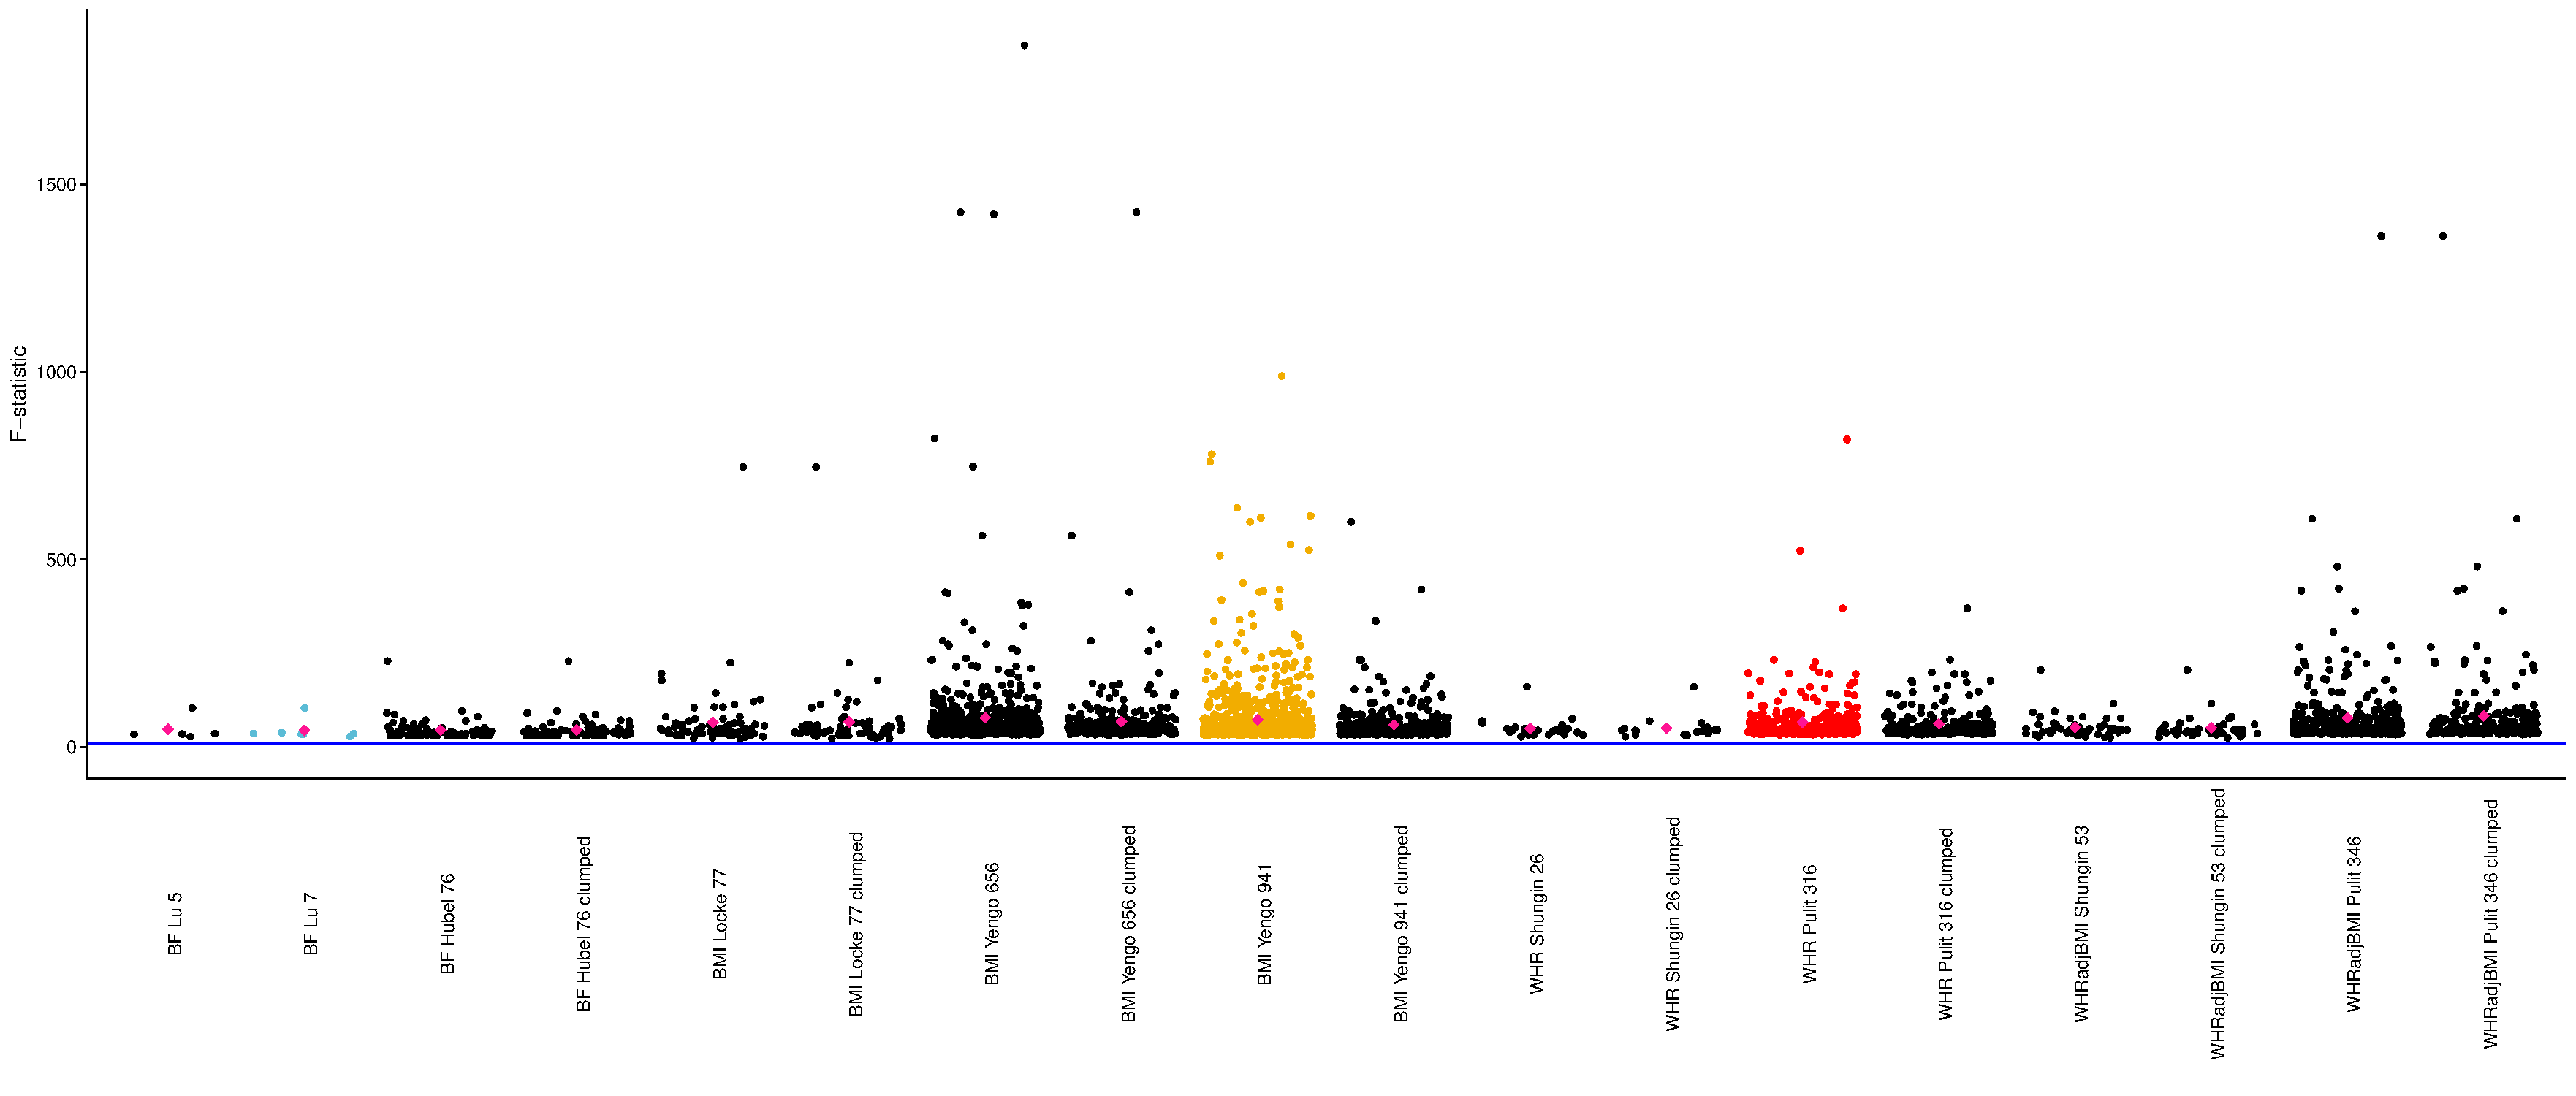
\includegraphics[width=1\linewidth]{../../002_adiposity_metabolites/analysis/all_exposures_fstatistics} \caption{f-statistics for all exposures used in chapter 5}\label{fig:appendix-chapter5-figure-fstatistics}
\end{figure}
\noindent 
\bsmall
\emph{Mean f-statistic for each exposure indicated by the pink diamond. The blue line indicates a nominal threshold of 10. Exposures used in the main analysis are highlighted with coloured points. The name after each exposure trait represents the authors last name of the original GWAS publication for which each exposure was obtained. The number following the first authors last name represents the number of SNPs obtained from the original GWAS and included; clumped refers to this original number of SNPs having been pruned based on an LD R\textsuperscript{2} of \(0.001\). BMI = body mass index, WHR = wasit hip ratio, WHRadjBMI = wasit hip ratio adjusted for BMI, BF = body fat percentage.}
\esmall

\hypertarget{chapter5-appendix-correlations}{%
\subsubsection{Correlations}\label{chapter5-appendix-correlations}}

Consistency in effect direction and size was investigated using Spearman's correlations.
\begin{verbatim}
[1] "Correlations between exposures"
\end{verbatim}
\begin{verbatim}
                 BF_Lu_7 BMI_Yengo_941 WHR_Pulit_316
BF_Lu_7        1.0000000    -0.7012485    -0.7189189
BMI_Yengo_941 -0.7012485     1.0000000     0.9449575
WHR_Pulit_316 -0.7189189     0.9449575     1.0000000
\end{verbatim}
\hypertarget{sensitivity-analysis}{%
\subsubsection{Sensitivity analysis}\label{sensitivity-analysis}}

\hypertarget{method-comparison}{%
\paragraph{Method comparison}\label{method-comparison}}

For all method comparison Circos plots the outer track is the main analysis (IVW-MRE) result, and is coloured for the exposure for consistency with the main text of the thesis (BMI = yellow, WHR = red, BF = blue). Purple = MR Egger, green = Weighted median, orange = Weighted mode. Solid points represent a \emph{p-value} threshold of \(0.05/22\) having been met; however only directional consistency between the methods is of interest when comparing the IVW-MRE model to the sensitivity models.
\begin{figure}
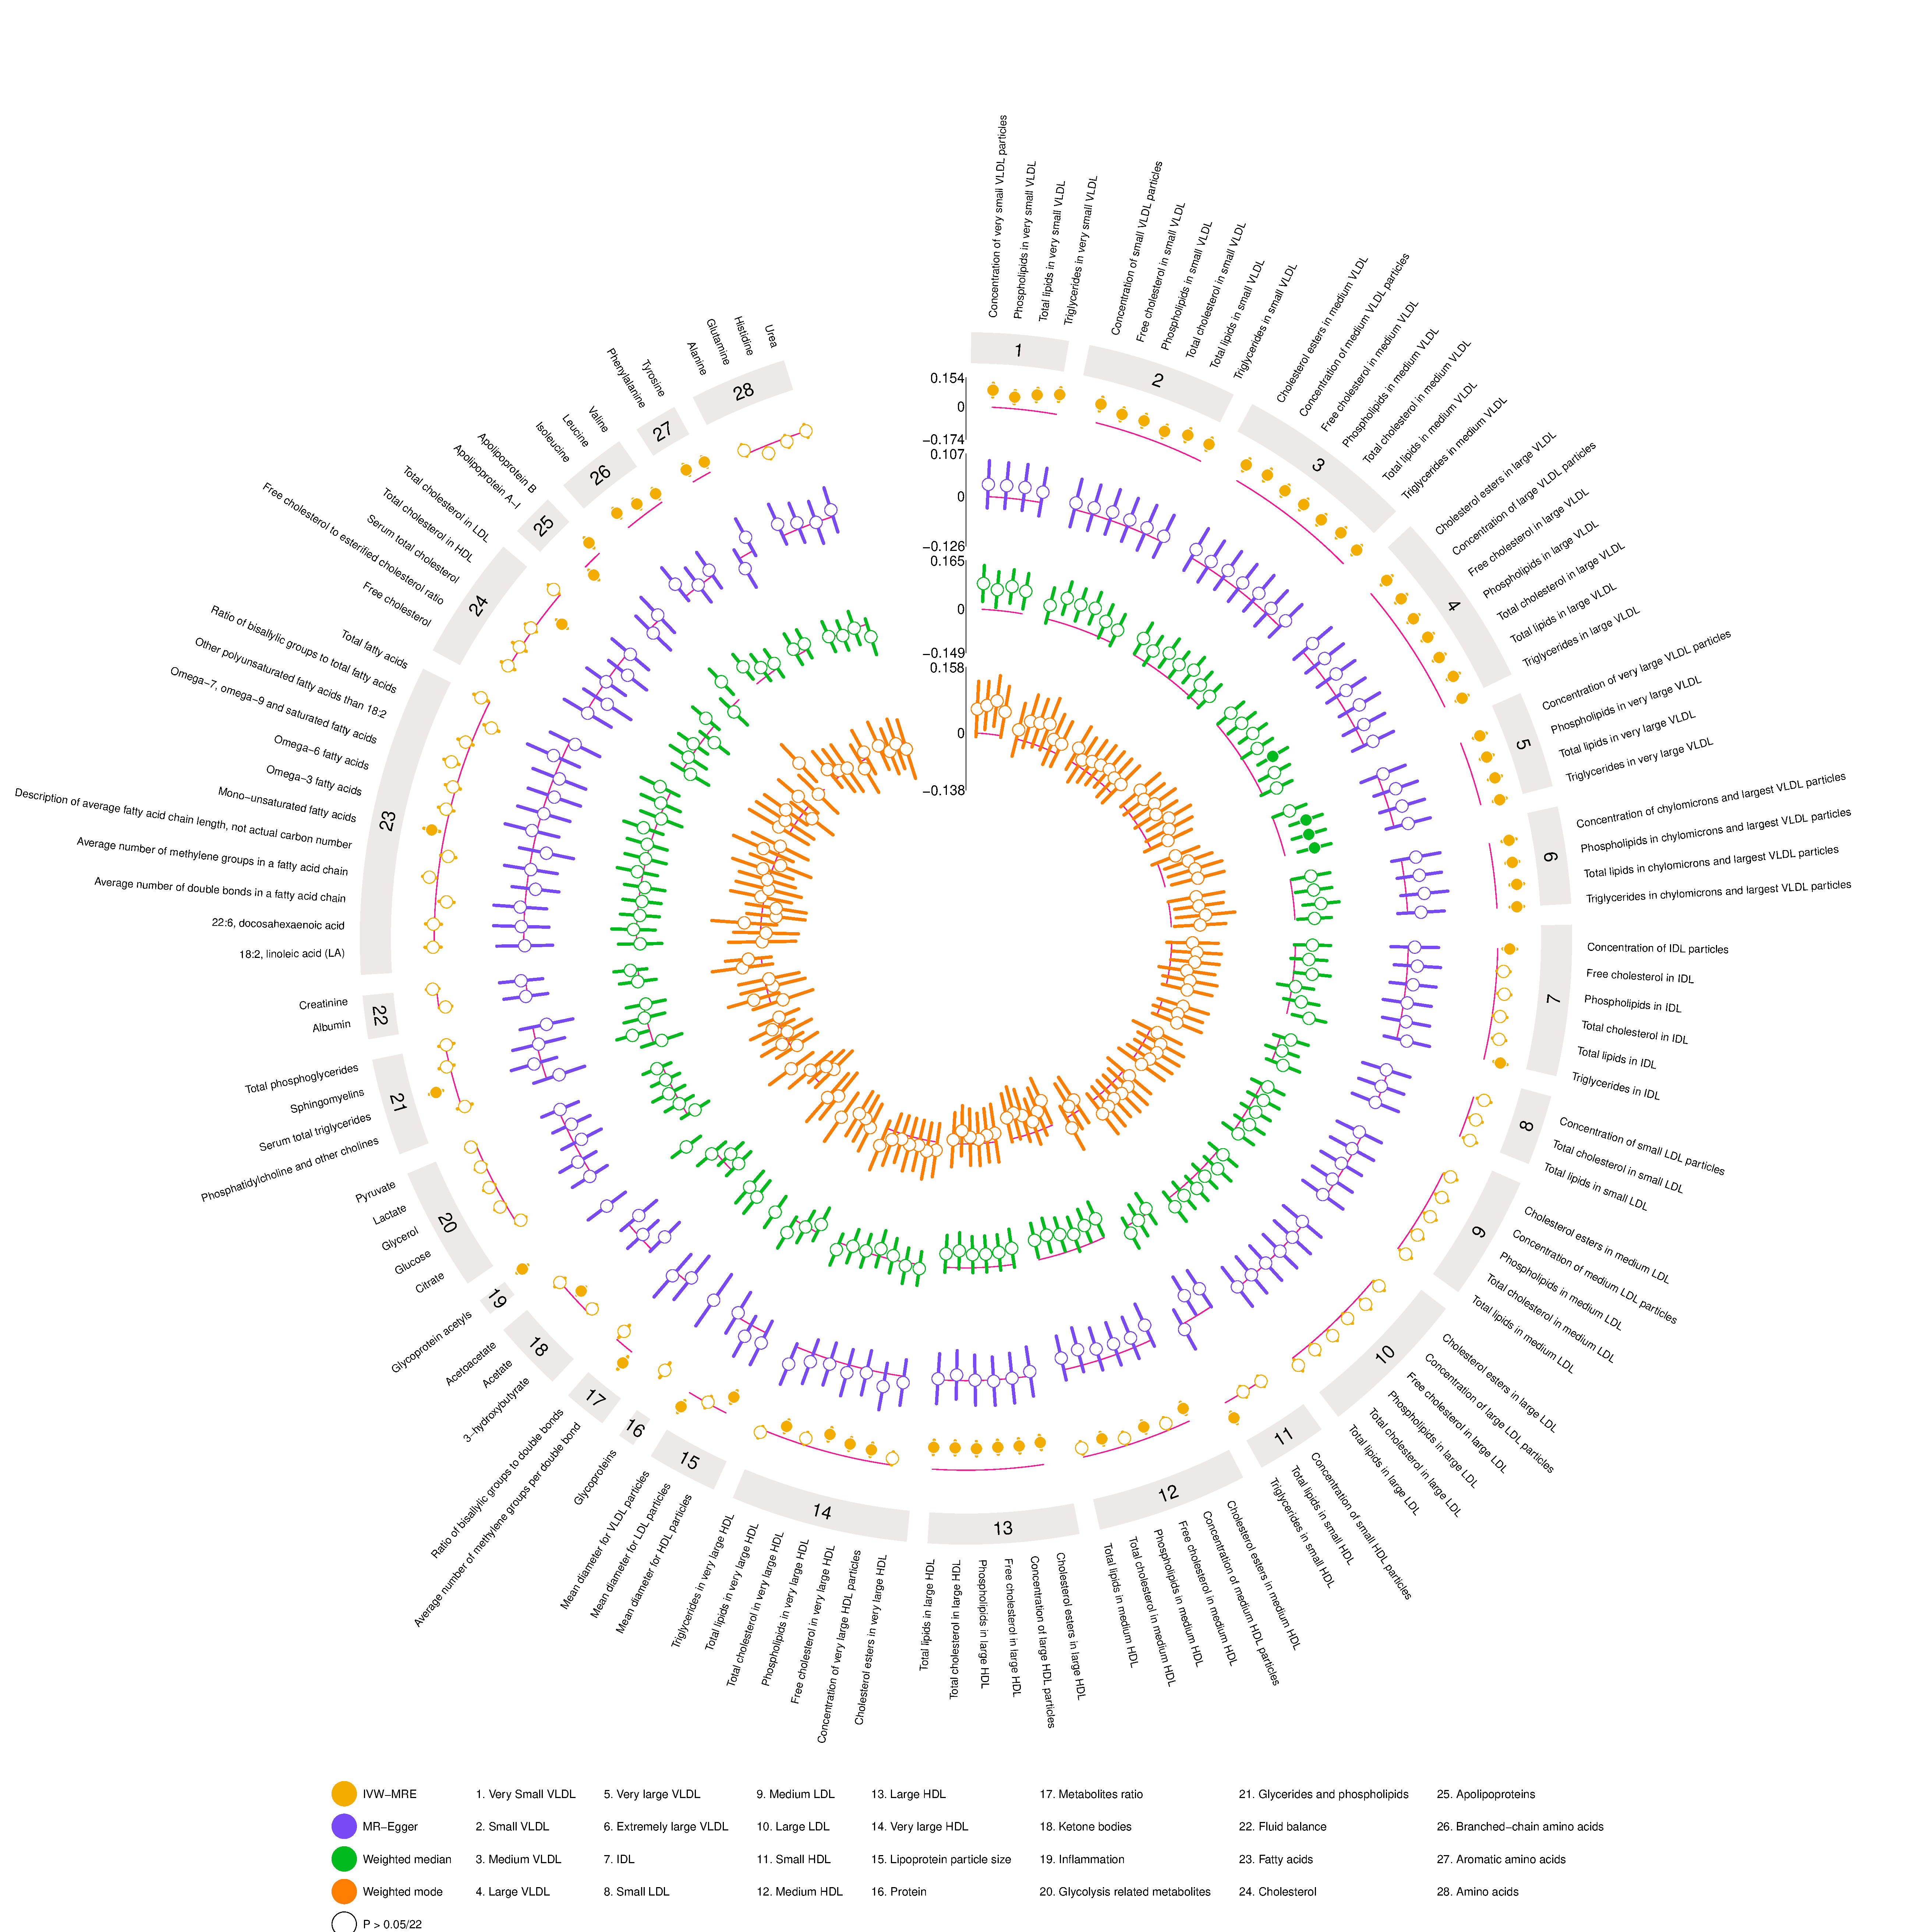
\includegraphics[width=1\linewidth]{data/chapter5/figures/sensitivity_analysis_BMI} \caption{Circosplot of main and sensitivity analysis for BMI}\label{fig:appendix-chapter5-figure-circosplot-sensitivity-main-BMI}
\end{figure}
\begin{figure}
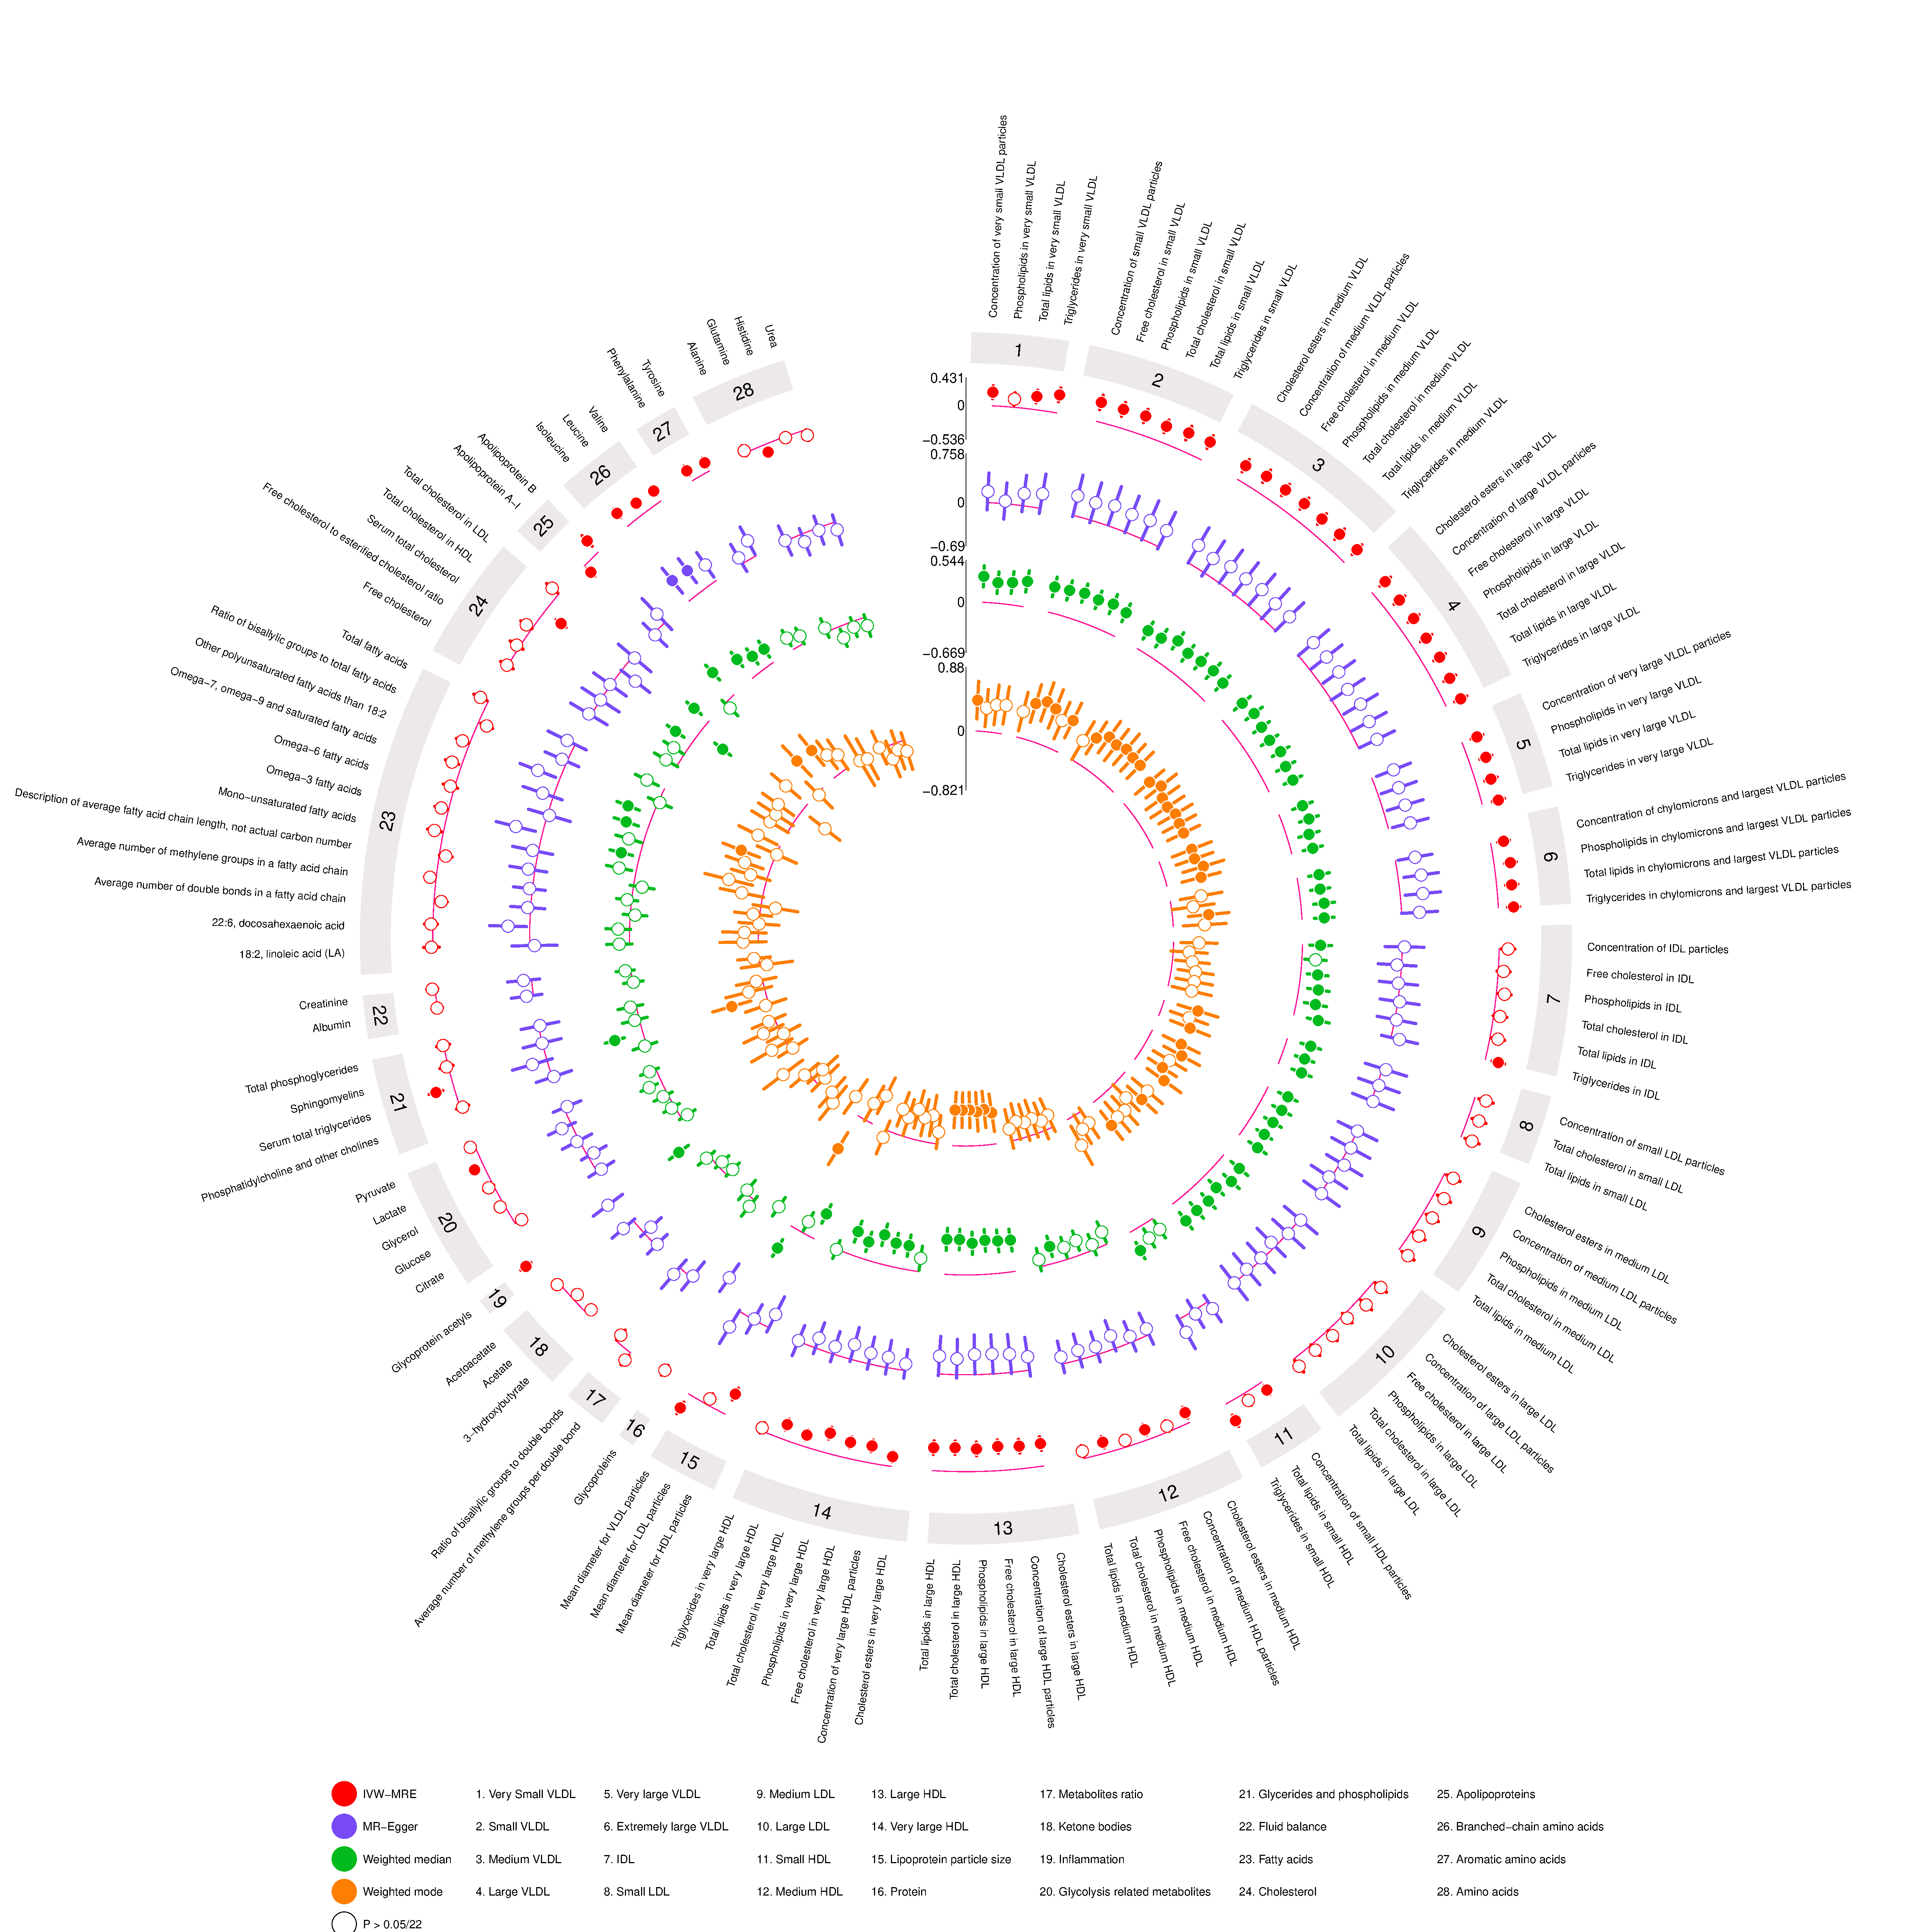
\includegraphics[width=1\linewidth]{data/chapter5/figures/sensitivity_analysis_WHR} \caption{Circosplot of main and sensitivity analysis for WHR}\label{fig:appendix-chapter5-figure-circosplot-sensitivity-main-WHR}
\end{figure}
\begin{figure}
\includegraphics[width=1\linewidth]{data/chapter5/figures/sensitivity_analysis_WHR} \caption{Circosplot of main and sensitivity analysis for BF}\label{fig:appendix-chapter5-figure-circosplot-sensitivity-main-BF}
\end{figure}
\hypertarget{representative-figures}{%
\paragraph{Representative figures}\label{representative-figures}}
\begin{figure}
\includegraphics[width=1\linewidth]{data/chapter5/figures/singlesnp_representative_figure} \caption{Single SNP MR results for BMI and glycerol - representative figure}\label{fig:appendix-chapter5-figure-singlesnp-representative-figure}
\end{figure}
\begin{figure}
\includegraphics[width=1\linewidth]{data/chapter5/figures/funnelplot_BMI_APOB_representative_figure} \caption{Funnel plot of single SNP MR results for BMI and Apolipoprotein B - representative figure}\label{fig:appendix-chapter5-figure-funnelplot-BMI-representative-figure}
\end{figure}
\begin{figure}
\includegraphics[width=1\linewidth]{data/chapter5/figures/funnelplot_BF_APOB_representative_figure} \caption{Funnel plot of single SNP MR results for BF and Apolipoprotein B - representative figure}\label{fig:appendix-chapter5-figure-funnelplot-BF-representative-figure}
\end{figure}
\begin{figure}
\includegraphics[width=1\linewidth]{data/chapter5/figures/leaveoneout_BF_representative_figure} \caption{Leave-one-iut results for BF and Acetoacetate - representative figure}\label{fig:appendix-chapter5-figure-leaveoneout-BF-representative-figure}
\end{figure}
\begin{figure}
\includegraphics[width=1\linewidth]{data/chapter5/figures/leaveoneout_BMI_representative_figure} \caption{Leave-one-iut results for BMI and Acetate - representative figure}\label{fig:appendix-chapter5-figure-leaveoneout-BMI-representative-figure}
\end{figure}
\hypertarget{chapter-6}{%
\section{Chapter 6}\label{chapter-6}}

\hypertarget{section-1}{%
\chapter{}\label{section-1}}

This first appendix includes all of the R chunks of code that were hidden throughout the document (using the \texttt{include\ =\ FALSE} chunk tag) to help with readibility and/or setup.

\textbf{In the main Rmd file}

This thesis was created using R Markdown. The template used here I have adapted from the R Markdown template here (\url{https://github.com/ismayc/thesisdown}), which is adapted from the Markdown template (\url{https://github.com/matlipson/phd_thesis_markdown}), which is an extension of Tom Pollards original Markdown for thesis work (\url{https://github.com/tompollard/phd_thesis_markdown}).

\hypertarget{section-2}{%
\chapter{}\label{section-2}}

Appendix B contains all of the code used throughout the thesis that is hidden from the reader using the \texttt{include\ =\ FALSE} chunk tag. This code is not necessary for reading, but is included here for completeness and transparency, and consists mainly of package installs and code to produce tables and figures included in the text.

To create the finished thesis file in R Markdown an index.Rmd file is used to compile multiple .Rmd files together. The index.Rmd file contains the YAML header, along with the following R code that installs and loads the neccessary packages to compile the thesis:
\begin{Shaded}
\begin{Highlighting}[]
\NormalTok{doc.type <-}\StringTok{ }\NormalTok{knitr}\OperatorTok{::}\NormalTok{opts_knit}\OperatorTok{$}\KeywordTok{get}\NormalTok{(}\StringTok{'rmarkdown.pandoc.to'}\NormalTok{)}
\KeywordTok{source}\NormalTok{(}\StringTok{"data/index/packages.R"}\NormalTok{)}
\end{Highlighting}
\end{Shaded}
\hypertarget{code-from-chapter-refchapter1}{%
\section{Code from Chapter \ref{chapter1}}\label{code-from-chapter-refchapter1}}

\hypertarget{code-from-chapter-refchapter2}{%
\section{Code from Chapter \ref{chapter2}}\label{code-from-chapter-refchapter2}}

\hypertarget{code-from-chapter-refchapter3}{%
\section{Code from Chapter \ref{chapter3}}\label{code-from-chapter-refchapter3}}

\hypertarget{code-from-chapter-refchapter4}{%
\section{Code from Chapter \ref{chapter4}}\label{code-from-chapter-refchapter4}}

\hypertarget{code-from-chapter-refchapter5}{%
\section{Code from Chapter \ref{chapter5}}\label{code-from-chapter-refchapter5}}

\hypertarget{code-from-chapter-refchapter6}{%
\section{Code from Chapter \ref{chapter6}}\label{code-from-chapter-refchapter6}}

\hypertarget{code-from-chapter-refchapter7}{%
\section{Code from Chapter \ref{chapter7}}\label{code-from-chapter-refchapter7}}

\hypertarget{code-from-chapter-refchapter8}{%
\section{Code from Chapter \ref{chapter8}}\label{code-from-chapter-refchapter8}}

\backmatter

\hypertarget{references}{%
\chapter*{References}\label{references}}
\addcontentsline{toc}{chapter}{References}

\markboth{References}{References}

\noindent

\hypertarget{refs}{}
\leavevmode\hypertarget{ref-WorldHealthOrganisation2018}{}%
1. World Health Organisation. \emph{Factsheet: Obesity and overweight}. (2018).

\leavevmode\hypertarget{ref-Stanaway2018}{}%
2. Stanaway, J. D. \emph{et al.} Global, regional, and national comparative risk assessment of 84 behavioural, environmental and occupational, and metabolic risks or clusters of risks for 195 countries and territories, 1990--2017: a systematic analysis for the Global Burden of Disease Stu. \emph{The Lancet} \textbf{392}, 1923--1994 (2018).

\leavevmode\hypertarget{ref-Ng2014}{}%
3. Ng, M. \emph{et al.} Global, regional, and national prevalence of overweight and obesity in children and adults during 1980-2013: a systematic analysis for the Global Burden of Disease Study 2013. \emph{Lancet (London, England)} \textbf{384}, 766--781 (2014).

\leavevmode\hypertarget{ref-NCD-RisC2016}{}%
4. (NCD-RisC), N. R. F. C. Trends in adult body-mass index in 200 countries from 1975 to 2014: a pooled analysis of 1698 population-based measurement studies with 192 million participants. \emph{The Lancet} \textbf{387}, 1377--1396 (2016).

\leavevmode\hypertarget{ref-Abarca-Gomez2017}{}%
5. Abarca-Gómez, L. \emph{et al.} Worldwide trends in body-mass index, underweight, overweight, and obesity from 1975 to 2016: a pooled analysis of 2416 population-based measurement studies in 128\&\#xb7;9 million children, adolescents, and adults. \emph{The Lancet} \textbf{390}, 2627--2642 (2017).

\leavevmode\hypertarget{ref-Ritchie2019}{}%
6. Ritchie, H. \& Roser, M. Obesity. Published online at OurWorldInData.org. Retrieved from: 'https://ourworldindata.org/obesity' {[}Online Resource{]} 05/12/2019. (2019).

\leavevmode\hypertarget{ref-WHO1995}{}%
7. WHO. Physical Status: The Use and Interpretation of Anthropometry: Report of a World Health Organization (WHO) Expert Committee. \emph{Geneva, Switzerland: World Health Organization} (1995).

\leavevmode\hypertarget{ref-WHO2000}{}%
8. WHO. Obesity: preventing and managing the global epidemic. Report of a WHO Consultation. \emph{Geneva, Switzerland: World Health Organization} (2000).

\leavevmode\hypertarget{ref-Pischon2008}{}%
9. Pischon, T. \emph{et al.} General and Abdominal Adiposity and Risk of Death in Europe. \emph{New England Journal of Medicine} \textbf{359}, 2105--2120 (2008).

\leavevmode\hypertarget{ref-Romero-Corral2008}{}%
10. Romero-Corral, A. \emph{et al.} Accuracy of body mass index in diagnosing obesity in the adult general population. \emph{International Journal of Obesity} \textbf{32}, 959--966 (2008).

\leavevmode\hypertarget{ref-Okorodudu2010}{}%
11. Okorodudu, D. O. \emph{et al.} Diagnostic performance of body mass index to identify obesity as defined by body adiposity: a systematic review and meta-analysis. \emph{International Journal of Obesity} \textbf{34}, 791--799 (2010).

\leavevmode\hypertarget{ref-Pasco2012}{}%
12. Pasco, J. A., Nicholson, G. C., Brennan, S. L. \& Kotowicz, M. A. Prevalence of obesity and the relationship between the body mass index and body fat: Cross-sectional, population-based data. \emph{PLoS ONE} \textbf{7}, (2012).

\leavevmode\hypertarget{ref-Prentice2001}{}%
13. Prentice, A. M. \& Jebb, S. A. Beyond body mass index. \emph{Obesity Reviews} \textbf{2}, 141--147 (2001).

\leavevmode\hypertarget{ref-Flegal2013}{}%
14. Flegal, K. M., Kit, B. K., Orpana, H. \& Graubard, B. I. Association of all-cause mortality with overweight and obesity using standard body mass index categories: a systematic review and meta-analysis. \emph{JAMA} \textbf{309}, 71--82 (2013).

\leavevmode\hypertarget{ref-Lee2015}{}%
15. Lee, J., Meyerhardt, J. A., Giovannucci, E. \& Jeon, J. Y. Association between body mass index and prognosis of colorectal cancer: a meta-analysis of prospective cohort studies. \emph{PloS one} \textbf{10}, e0120706--e0120706 (2015).

\leavevmode\hypertarget{ref-Elagizi2018}{}%
16. Elagizi, A. \emph{et al.} An Overview and Update on Obesity and the Obesity Paradox in Cardiovascular Diseases. \emph{Progress in Cardiovascular Diseases} \textbf{61}, 142--150 (2018).

\leavevmode\hypertarget{ref-Banack2013}{}%
17. Banack, H. R. \& Kaufman, J. S. The `Obesity Paradox' Explained. \emph{Epidemiology} \textbf{24}, (2013).

\leavevmode\hypertarget{ref-Willett2013}{}%
18. Willett, W. C., Hu, F. B. \& Thun, M. Overweight, Obesity, and All-Cause Mortality. \emph{JAMA} \textbf{309}, 1681--1682 (2013).

\leavevmode\hypertarget{ref-Khan2018}{}%
19. Khan, S. S. \emph{et al.} Association of Body Mass Index With Lifetime Risk of Cardiovascular Disease and Compression of Morbidity. \emph{JAMA Cardiology} \textbf{3}, 280--287 (2018).

\leavevmode\hypertarget{ref-Sahakyan2015}{}%
20. Sahakyan, K. R. \emph{et al.} Normal-Weight Central Obesity: Implications for Total and Cardiovascular Mortality. \emph{Annals of internal medicine} \textbf{163}, 827--835 (2015).

\leavevmode\hypertarget{ref-Hamer2017}{}%
21. Hamer, M., O'Donovan, G., Stensel, D. \& Stamatakis, E. Normal-Weight Central Obesity and Risk for Mortality. \emph{Annals of Internal Medicine} \textbf{166}, 917--918 (2017).

\leavevmode\hypertarget{ref-WorldHealthOrganisation2008}{}%
22. World Health Organisation. \emph{Waist Circumference and Waist-Hip Ratio: Report of a WHO Expert Consultation}. (WHO, 2008).

\leavevmode\hypertarget{ref-Collaboration2009}{}%
23. Prospective Studies Collaboration \emph{et al.} Body-mass index and cause-specific mortality in 900 000 adults: collaborative analyses of 57 prospective studies. \emph{Lancet (London, England)} \textbf{373}, 1083--1096 (2009).

\leavevmode\hypertarget{ref-WHO2008}{}%
24. WHO. Waist Circumference and Waist-Hip Ratio: Report of a WHO Expert Consultation. \emph{Geneva, Switzerland: World Health Organization} (2008).

\leavevmode\hypertarget{ref-WorldHealthOrganisation2000}{}%
25. World Health Organisation. \emph{Obesity : preventing and managing the global epidemic : report of a WHO consultation}. (WHO, 2000).

\leavevmode\hypertarget{ref-Jebb2000}{}%
26. Jebb, S. A., Cole, T. J., Doman, D., Murgatroyd, P. R. \& Prentice, A. M. Evaluation of the novel Tanita body-fat analyser to measure body composition by comparison with a four-compartment model. \emph{British Journal of Nutrition} \textbf{83}, 115--122 (2000).

\leavevmode\hypertarget{ref-Chouinard2007}{}%
27. Chouinard, L. E. \emph{et al.} Bioelectrical Impedance vs. Four-compartment Model to Assess Body Fat Change in Overweight Adults. \emph{Obesity} \textbf{15}, 85--92 (2007).

\leavevmode\hypertarget{ref-Tallroth2013}{}%
28. Tallroth, K., Kettunen, J. A. \& Kujala, U. M. Reproducibility of Regional DEXA Examinations of Abdominal Fat and Lean Tissue. \emph{Obesity Facts} \textbf{6}, 203--210 (2013).

\leavevmode\hypertarget{ref-Jenkins2018}{}%
29. Jenkins, D. A. \emph{et al.} Adiposity-Mortality Relationships in Type 2 Diabetes, Coronary Heart Disease, and Cancer Subgroups in the UK Biobank, and Their Modification by Smoking. \emph{Diabetes Care} \textbf{41}, 1878 LP--1886 (2018).

\leavevmode\hypertarget{ref-Rost2018}{}%
30. Rost, S. \emph{et al.} New indexes of body fat distribution and sex-specific risk of total and cause-specific mortality: a prospective cohort study. \emph{BMC Public Health} \textbf{18}, 427 (2018).

\leavevmode\hypertarget{ref-Muxf8rkedal2011}{}%
31. Mørkedal, B., Romundstad, P. R. \& Vatten, L. J. Informativeness of indices of blood pressure, obesity and serum lipids in relation to ischaemic heart disease mortality: the HUNT-II study. \emph{European journal of epidemiology} \textbf{26}, 457--461 (2011).

\leavevmode\hypertarget{ref-Dong2018}{}%
32. Dong, B. \emph{et al.} Joint association between body fat and its distribution with all-cause mortality: A data linkage cohort study based on NHANES (1988-2011). \emph{PloS one} \textbf{13}, e0193368--e0193368 (2018).

\leavevmode\hypertarget{ref-Lee2018}{}%
33. Lee, D. H. \emph{et al.} Predicted lean body mass, fat mass, and all cause and cause specific mortality in men: prospective US cohort study. \emph{BMJ} \textbf{362}, k2575 (2018).

\leavevmode\hypertarget{ref-Bigaard2004}{}%
34. Bigaard, J. \emph{et al.} Body Fat and Fat-Free Mass and All-Cause Mortality. \emph{Obesity Research} \textbf{12}, 1042--1049 (2004).

\leavevmode\hypertarget{ref-Barberio2019}{}%
35. Barberio, A. M. \emph{et al.} Central body fatness is a stronger predictor of cancer risk than overall body size. \emph{Nature Communications} \textbf{10}, 383 (2019).

\leavevmode\hypertarget{ref-Dobbelsteyn2001}{}%
36. Dobbelsteyn, C. J., Joffres, M. R., MacLean, D. R., Flowerdew, G. \& Group, T. C. H. H. S. R. A comparative evaluation of waist circumference, waist-to-hip ratio and body mass index as indicators of cardiovascular risk factors. The Canadian Heart Health Surveys. \emph{International Journal of Obesity} \textbf{25}, 652--661 (2001).

\leavevmode\hypertarget{ref-Yusuf2005}{}%
37. Yusuf, S. \emph{et al.} Obesity and the risk of myocardial infarction in 27,000 participants from 52 countries: a case-control study. \emph{The Lancet} \textbf{366}, 1640--1649 (2005).

\leavevmode\hypertarget{ref-Elsayed2008}{}%
38. Elsayed, E. F. \emph{et al.} Waist-to-hip ratio, body mass index, and subsequent kidney disease and death. \emph{American journal of kidney diseases : the official journal of the National Kidney Foundation} \textbf{52}, 29--38 (2008).

\leavevmode\hypertarget{ref-Sahlman2020}{}%
39. Sahlman, P. \emph{et al.} Genetic and lifestyle risk factors for advanced liver disease among men and women. \emph{Journal of gastroenterology and hepatology} \textbf{35}, 291--298 (2020).

\leavevmode\hypertarget{ref-Wiltink2013}{}%
40. Wiltink, J. \emph{et al.} Associations between depression and different measures of obesity (BMI, WC, WHtR, WHR). \emph{BMC psychiatry} \textbf{13}, 223 (2013).

\leavevmode\hypertarget{ref-Dye2017}{}%
41. Dye, L., Boyle, N. B., Champ, C. \& Lawton, C. The relationship between obesity and cognitive health and decline. \emph{The Proceedings of the Nutrition Society} \textbf{76}, 443--454 (2017).

\leavevmode\hypertarget{ref-Basraon2016}{}%
42. Basraon, S. K. \emph{et al.} Relationship of Early Pregnancy Waist-to-Hip Ratio versus Body Mass Index with Gestational Diabetes Mellitus and Insulin Resistance. \emph{American journal of perinatology} \textbf{33}, 114--121 (2016).

\leavevmode\hypertarget{ref-Price2006a}{}%
43. Price, G. M., Uauy, R., Breeze, E., Bulpitt, C. J. \& Fletcher, A. E. Weight, shape, and mortality risk in older persons: elevated waist-hip ratio, not high body mass index, is associated with a greater risk of death. \emph{The American journal of clinical nutrition} \textbf{84}, 449--460 (2006).

\leavevmode\hypertarget{ref-Qiao2010}{}%
44. Qiao, Q. \& Nyamdorj, R. Is the association of type II diabetes with waist circumference or waist-to-hip ratio stronger than that with body mass index?. \emph{European journal of clinical nutrition} \textbf{64}, 30--34 (2010).

\leavevmode\hypertarget{ref-Romero-Corral2010}{}%
45. Romero-Corral, A. \emph{et al.} Normal weight obesity: a risk factor for cardiometabolic dysregulation and cardiovascular mortality. \emph{European heart journal} \textbf{31}, 737--746 (2010).

\leavevmode\hypertarget{ref-Oh2014}{}%
46. Oh, S. W. \emph{et al.} Relationship between changes in body fat and a decline of renal function in the elderly. \emph{PloS one} \textbf{9}, e84052--e84052 (2014).

\leavevmode\hypertarget{ref-Jo2018}{}%
47. Jo, A. \& Mainous III, A. G. Informational value of percent body fat with body mass index for the risk of abnormal blood glucose: a nationally representative cross-sectional study. \emph{BMJ Open} \textbf{8}, e019200 (2018).

\leavevmode\hypertarget{ref-Frayn2003}{}%
48. Frayn, K. N., Karpe, F., Fielding, B. A., Macdonald, I. A. \& Coppack, S. W. Integrative physiology of human adipose tissue. \emph{International Journal of Obesity} \textbf{27}, 875--888 (2003).

\leavevmode\hypertarget{ref-Cohen2016}{}%
49. Cohen, P. \& Spiegelman, B. M. Cell biology of fat storage. \emph{Molecular biology of the cell} \textbf{27}, 2523--2527 (2016).

\leavevmode\hypertarget{ref-Luo2016}{}%
50. Luo, L. \& Liu, M. Adipose tissue in control of metabolism. \emph{Journal of Endocrinology} \textbf{231}, R77--R99 (2016).

\leavevmode\hypertarget{ref-Kershaw2004}{}%
51. Kershaw, E. E. \& Flier, J. S. Adipose Tissue as an Endocrine Organ. \emph{The Journal of Clinical Endocrinology \& Metabolism} \textbf{89}, 2548--2556 (2004).

\leavevmode\hypertarget{ref-Dahlman2010}{}%
52. Dahlman, I. \& Arner, P. Chapter 3 - Genetics of Adipose Tissue Biology. in \emph{Genes and obesity} (eds. Bouchard, C. B. T. P. in M. B. \& Science, T.) \textbf{94}, 39--74 (Academic Press, 2010).

\leavevmode\hypertarget{ref-Galgani2008}{}%
53. Galgani, J. \& Ravussin, E. Energy metabolism, fuel selection and body weight regulation. \emph{International journal of obesity (2005)} \textbf{32 Suppl 7}, S109--S119 (2008).

\leavevmode\hypertarget{ref-Amitani2013}{}%
54. Amitani, M., Asakawa, A., Amitani, H. \& Inui, A. The role of leptin in the control of insulin-glucose axis. \textbf{7}, 51 (2013).

\leavevmode\hypertarget{ref-Gray2007}{}%
55. Gray, S. L. \& Vidal-Puig, A. J. Adipose Tissue Expandability in the Maintenance of Metabolic Homeostasis. \emph{Nutrition Reviews} \textbf{65}, S7--S12 (2007).

\leavevmode\hypertarget{ref-Cannon2004}{}%
56. Cannon, B. \& Nedergaard, J. A. N. Brown Adipose Tissue: Function and Physiological Significance. \emph{Physiological Reviews} \textbf{84}, 277--359 (2004).

\leavevmode\hypertarget{ref-Lee2014}{}%
57. Lee, J.-E. \& Ge, K. Transcriptional and epigenetic regulation of PPAR\(\gamma\) expression during adipogenesis. \emph{Cell \& Bioscience} \textbf{4}, 29 (2014).

\leavevmode\hypertarget{ref-Schreiber2019}{}%
58. Schreiber, R., Xie, H. \& Schweiger, M. Of mice and men: The physiological role of adipose triglyceride lipase (ATGL). \emph{Biochimica et Biophysica Acta (BBA) - Molecular and Cell Biology of Lipids} \textbf{1864}, 880--899 (2019).

\leavevmode\hypertarget{ref-Lehr2012}{}%
59. Lehr, S., Hartwig, S. \& Sell, H. Adipokines: A treasure trove for the discovery of biomarkers for metabolic disorders. \emph{PROTEOMICS -- Clinical Applications} \textbf{6}, 91--101 (2012).

\leavevmode\hypertarget{ref-Fasshauer2015}{}%
60. Fasshauer, M. \& Blüher, M. Adipokines in health and disease. \emph{Trends in Pharmacological Sciences} \textbf{36}, 461--470 (2015).

\leavevmode\hypertarget{ref-Bluher2013}{}%
61. Blüher, M. Adipose tissue dysfunction contributes to obesity related metabolic diseases. \emph{Best Practice \& Research Clinical Endocrinology \& Metabolism} \textbf{27}, 163--177 (2013).

\leavevmode\hypertarget{ref-Bluher2015}{}%
62. Blüher, M. \& Mantzoros, C. S. From leptin to other adipokines in health and disease: Facts and expectations at the beginning of the 21st century. \emph{Metabolism} \textbf{64}, 131--145 (2015).

\leavevmode\hypertarget{ref-Pan2018}{}%
63. Pan, W. W. \& Myers, M. G. Leptin and the maintenance of elevated body weight. \emph{Nature Reviews Neuroscience} \textbf{19}, 95--105 (2018).

\leavevmode\hypertarget{ref-Ahn2019}{}%
64. Ahn, J., Wu, H. \& Lee, K. Integrative Analysis Revealing Human Adipose-Specific Genes and Consolidating Obesity Loci. \emph{Scientific Reports} \textbf{9}, 3087 (2019).

\leavevmode\hypertarget{ref-Achari2017}{}%
65. Achari, E. A. \& Jain, K. S. Adiponectin, a Therapeutic Target for Obesity, Diabetes, and Endothelial Dysfunction. \textbf{18}, (2017).

\leavevmode\hypertarget{ref-Lefterova2009}{}%
66. Lefterova, M. I. \& Lazar, M. A. New developments in adipogenesis. \emph{Trends in Endocrinology \& Metabolism} \textbf{20}, 107--114 (2009).

\leavevmode\hypertarget{ref-Maguire2018}{}%
67. Maguire, D., Talwar, D., Shiels, P. G. \& McMillan, D. The role of thiamine dependent enzymes in obesity and obesity related chronic disease states: A systematic review. \emph{Clinical Nutrition ESPEN} \textbf{25}, 8--17 (2018).

\leavevmode\hypertarget{ref-Ma2013a}{}%
68. Ma, R. C. W. \& Chan, J. C. N. Type 2 diabetes in East Asians: similarities and differences with populations in Europe and the United States. \emph{Annals of the New York Academy of Sciences} \textbf{1281}, 64--91 (2013).

\leavevmode\hypertarget{ref-Bray2004}{}%
69. Bray, G. A. Medical Consequences of Obesity. \emph{The Journal of Clinical Endocrinology \& Metabolism} \textbf{89}, 2583--2589 (2004).

\leavevmode\hypertarget{ref-Haslam2005}{}%
70. Haslam, D. W. \& James, W. P. T. Obesity. \emph{The Lancet} \textbf{366}, 1197--1209 (2005).

\leavevmode\hypertarget{ref-Poulain2006}{}%
71. Poulain, M. \emph{et al.} The effect of obesity on chronic respiratory diseases: pathophysiology and therapeutic strategies. \emph{CMAJ : Canadian Medical Association journal = journal de l'Association medicale canadienne} \textbf{174}, 1293--1299 (2006).

\leavevmode\hypertarget{ref-Carreras-Torres2018}{}%
72. Carreras-Torres, R. \emph{et al.} Role of obesity in smoking behaviour: Mendelian randomisation study in UK Biobank. \emph{BMJ} \textbf{361}, k1767 (2018).

\leavevmode\hypertarget{ref-Jayedi2018}{}%
73. Jayedi, A., Rashidy-Pour, A., Khorshidi, M. \& Shab-Bidar, S. Body mass index, abdominal adiposity, weight gain and risk of developing hypertension: a systematic review and dose--response meta-analysis of more than 2.3 million participants. \emph{Obesity Reviews} \textbf{19}, 654--667 (2018).

\leavevmode\hypertarget{ref-Bhaskaran2014}{}%
74. Bhaskaran, K. \emph{et al.} Body-mass index and risk of 22 specific cancers: a population-based cohort study of 524 million UK adults. \emph{Lancet (London, England)} \textbf{384}, 755--765 (2014).

\leavevmode\hypertarget{ref-Dagfinn2016}{}%
75. Dagfinn, A. \emph{et al.} Body Mass Index, Abdominal Fatness, and Heart Failure Incidence and Mortality. \emph{Circulation} \textbf{133}, 639--649 (2016).

\leavevmode\hypertarget{ref-DaveySmith2014}{}%
76. Davey Smith, G. \& Hemani, G. Mendelian randomization: genetic anchors for causal inference in epidemiological studies. \emph{Human Molecular Genetics} \textbf{23}, R89--R98 (2014).

\leavevmode\hypertarget{ref-Timpson2005}{}%
77. Timpson, N. J. \emph{et al.} C-reactive protein and its role in metabolic syndrome: mendelian randomisation study. \emph{Lancet} \textbf{366}, 1954--1959 (2005).

\leavevmode\hypertarget{ref-CCGC2011}{}%
78. (CCGC), C. R. P. C. H. D. G. C. \emph{et al.} Association between C reactive protein and coronary heart disease: mendelian randomisation analysis based on individual participant data. \emph{BMJ (Clinical research ed.)} \textbf{342}, d548--d548 (2011).

\leavevmode\hypertarget{ref-Yarmolinsky2018}{}%
79. Yarmolinsky, J. \emph{et al.} Circulating Selenium and Prostate Cancer Risk: A Mendelian Randomization Analysis. \emph{Journal of the National Cancer Institute} \textbf{110}, 1035--1038 (2018).

\leavevmode\hypertarget{ref-DaveySmith2003}{}%
80. Davey Smith, G. \& Ebrahim, S. `Mendelian randomization': can genetic epidemiology contribute to understanding environmental determinants of disease?*. \emph{International Journal of Epidemiology} \textbf{32}, 1--22 (2003).

\leavevmode\hypertarget{ref-Davies2018}{}%
81. Davies, N. M., Holmes, M. V. \& Davey Smith, G. Reading Mendelian randomisation studies: a guide, glossary, and checklist for clinicians. \emph{BMJ} \textbf{362}, k601 (2018).

\leavevmode\hypertarget{ref-Burgess2015}{}%
82. Burgess, S., Timpson, N. J., Ebrahim, S. \& Davey Smith, G. Mendelian randomization: where are we now and where are we going? \emph{International Journal of Epidemiology} \textbf{44}, 379--388 (2015).

\leavevmode\hypertarget{ref-Bowden2019}{}%
83. Bowden, J. \& Holmes, M. V. Meta-analysis and Mendelian randomization: A review. \emph{Research Synthesis Methods} \textbf{0}, (2019).

\leavevmode\hypertarget{ref-Lawlor2019}{}%
84. Lawlor, D. A. \emph{et al.} A Mendelian Randomization dictionary: Useful definitions and descriptions for undertaking, understanding and interpreting Mendelian Randomization studies. \emph{OSF Preprints} (2019). doi:\href{https://doi.org/10.31219/osf.io/6yzs7}{10.31219/osf.io/6yzs7}

\leavevmode\hypertarget{ref-Smith2004}{}%
85. Smith, G. D. \& Ebrahim, S. Mendelian randomization: prospects, potentials, and limitations. \emph{Int J Epidemiol} \textbf{33}, 30--42 (2004).

\leavevmode\hypertarget{ref-Hartwig2018}{}%
86. Hartwig, F. P., Davies, N. M. \& Davey Smith, G. Bias in Mendelian randomization due to assortative mating. \emph{Genetic epidemiology} \textbf{42}, 608--620 (2018).

\leavevmode\hypertarget{ref-Brumpton2019}{}%
87. Brumpton, B. \emph{et al.} Within-family studies for Mendelian randomization: avoiding dynastic, assortative mating, and population stratification biases. \emph{bioRxiv} 602516 (2019). doi:\href{https://doi.org/10.1101/602516}{10.1101/602516}

\leavevmode\hypertarget{ref-Sanderson2019}{}%
88. Sanderson, E., Davey Smith, G., Bowden, J. \& Munafò, M. R. Mendelian randomisation analysis of the effect of educational attainment and cognitive ability on smoking behaviour. \emph{Nature Communications} \textbf{10}, 2949 (2019).

\leavevmode\hypertarget{ref-Haworth2019}{}%
89. Haworth, S. \emph{et al.} Apparent latent structure within the UK Biobank sample has implications for epidemiological analysis. \emph{Nature Communications} \textbf{10}, 333 (2019).

\leavevmode\hypertarget{ref-Berg2019}{}%
90. Berg, J. J. \emph{et al.} Reduced signal for polygenic adaptation of height in UK Biobank. \emph{eLife} \textbf{8}, e39725 (2019).

\leavevmode\hypertarget{ref-Smith2010}{}%
91. Smith, G. D. Mendelian Randomization for Strengthening Causal Inference in Observational Studies: Application to Gene × Environment Interactions. \emph{Perspectives on Psychological Science} \textbf{5}, 527--545 (2010).

\leavevmode\hypertarget{ref-Geiler-Samerotte2019}{}%
92. Geiler-Samerotte, K., Sartori, F. M. O. \& Siegal, M. L. Decanalizing thinking on genetic canalization. \emph{Seminars in cell \& developmental biology} \textbf{88}, 54--66 (2019).

\leavevmode\hypertarget{ref-Pierce2013}{}%
93. Pierce, B. L. \& Burgess, S. Efficient Design for Mendelian Randomization Studies: Subsample and 2-Sample Instrumental Variable Estimators. \emph{American Journal of Epidemiology} \textbf{178}, 1177--1184 (2013).

\leavevmode\hypertarget{ref-Speliotes2010a}{}%
94. Speliotes, E. K. \emph{et al.} Association analyses of 249,796 individuals reveal 18 new loci associated with body mass index. \emph{Nat Genet} \textbf{42}, 937--948 (2010).

\leavevmode\hypertarget{ref-Shungin2015}{}%
95. Shungin, D. \emph{et al.} New genetic loci link adipose and insulin biology to body fat distribution. \emph{Nature} \textbf{518}, 187--196 (2015).

\leavevmode\hypertarget{ref-Locke2015}{}%
96. Locke, A. E. \emph{et al.} Genetic studies of body mass index yield new insights for obesity biology. \emph{Nature} \textbf{518}, 197--206 (2015).

\leavevmode\hypertarget{ref-Pulit2019}{}%
97. Pulit, S. L. \emph{et al.} Meta-analysis of genome-wide association studies for body fat distribution in 694~649 individuals of European ancestry. \emph{Human molecular genetics} \textbf{28}, 166--174 (2019).

\leavevmode\hypertarget{ref-Yengo2018}{}%
98. Yengo, L. \emph{et al.} Meta-analysis of genome-wide association studies for height and body mass index in 700000 individuals of European ancestry. \emph{Human molecular genetics} \textbf{27}, 3641--3649 (2018).

\leavevmode\hypertarget{ref-Sohail2019}{}%
99. Sohail, M. \emph{et al.} Polygenic adaptation on height is overestimated due to uncorrected stratification in genome-wide association studies. \emph{eLife} \textbf{8}, e39702 (2019).

\leavevmode\hypertarget{ref-Boyle2017}{}%
100. Boyle, E. A., Li, Y. I. \& Pritchard, J. K. An Expanded View of Complex Traits: From Polygenic to Omnigenic. \emph{Cell} \textbf{169}, 1177--1186 (2017).

\leavevmode\hypertarget{ref-Liu2019}{}%
101. Liu, X., Li, Y. I. \& Pritchard, J. K. Trans Effects on Gene Expression Can Drive Omnigenic Inheritance. \emph{Cell} \textbf{177}, 1022--1034.e6 (2019).

\leavevmode\hypertarget{ref-GTEx2013}{}%
102. The GTEx Consortium. The Genotype-Tissue Expression (GTEx) project. \emph{Nature genetics} \textbf{45}, 580--585 (2013).

\leavevmode\hypertarget{ref-Carter2020}{}%
103. Carter, A. R. \emph{et al.} Mendelian randomisation for mediation analysis: current methods and challenges for implementation. \emph{bioRxiv} 835819 (2020). doi:\href{https://doi.org/10.1101/835819}{10.1101/835819}

\leavevmode\hypertarget{ref-Relton2012}{}%
104. Relton, C. L. \& Davey Smith, G. Two-step epigenetic Mendelian randomization: a strategy for establishing the causal role of epigenetic processes in pathways to disease. \emph{Int J Epidemiol} \textbf{41}, 161--176 (2012).

\leavevmode\hypertarget{ref-Burgess2015b}{}%
105. Burgess, S., Daniel, R. M., Butterworth, A. S., Thompson, S. G. \& Consortium, E.-I. Network Mendelian randomization: using genetic variants as instrumental variables to investigate mediation in causal pathways. \emph{International journal of epidemiology} \textbf{44}, 484--495 (2015).

\leavevmode\hypertarget{ref-Sanderson2018}{}%
106. Sanderson, E., Davey Smith, G., Windmeijer, F. \& Bowden, J. An examination of multivariable Mendelian randomization in the single-sample and two-sample summary data settings. \emph{International Journal of Epidemiology} \textbf{48}, 713--727 (2018).

\leavevmode\hypertarget{ref-VanderWeele2016}{}%
107. VanderWeele, T. J. Mediation Analysis: A Practitioner's Guide. \emph{Annual Review of Public Health} \textbf{37}, 17--32 (2016).

\leavevmode\hypertarget{ref-Varbo2015}{}%
108. Varbo, A. \emph{et al.} Remnant Cholesterol, Low-Density Lipoprotein Cholesterol, and Blood Pressure as Mediators From Obesity to Ischemic Heart Disease. \emph{Circulation Research} \textbf{116}, 665--673 (2015).

\leavevmode\hypertarget{ref-Xu2017}{}%
109. Xu, L., Borges, M. C., Hemani, G. \& Lawlor, D. A. The role of glycaemic and lipid risk factors in mediating the effect of BMI on coronary heart disease: a two-step, two-sample Mendelian randomisation study. \emph{Diabetologia} \textbf{60}, 2210--2220 (2017).

\leavevmode\hypertarget{ref-Marouli2019}{}%
110. Marouli, E. \emph{et al.} Mendelian randomisation analyses find pulmonary factors mediate the effect of height on coronary artery disease. \emph{Communications Biology} \textbf{2}, 119 (2019).

\leavevmode\hypertarget{ref-Carter2019}{}%
111. Carter, A. R. \emph{et al.} Understanding the consequences of education inequality on cardiovascular disease: mendelian randomisation study. \emph{BMJ} \textbf{365}, l1855 (2019).

\leavevmode\hypertarget{ref-Davies2019}{}%
112. Davies, N. M. \emph{et al.} Multivariable two-sample Mendelian randomization estimates of the effects of intelligence and education on health. \emph{eLife} \textbf{8}, e43990 (2019).

\leavevmode\hypertarget{ref-Richardson2019}{}%
113. Richardson, T. G. \emph{et al.} Apolipoprotein B underlies the causal relationship of circulating blood lipids with coronary heart disease. \emph{medRxiv} 19004895 (2019). doi:\href{https://doi.org/10.1101/19004895}{10.1101/19004895}

\leavevmode\hypertarget{ref-Johnson2019}{}%
114. Johnson, K. E. \emph{et al.} Assessing a causal relationship between circulating lipids and breast cancer risk: Mendelian randomization study. \emph{bioRxiv} 794594 (2019). doi:\href{https://doi.org/10.1101/794594}{10.1101/794594}

\leavevmode\hypertarget{ref-Griffin2006}{}%
115. Griffin, J. L. The Cinderella story of metabolic profiling: does metabolomics get to go to the functional genomics ball? \emph{Philosophical Transactions of the Royal Society B: Biological Sciences} \textbf{361}, 147--161 (2006).

\leavevmode\hypertarget{ref-Su2014}{}%
116. Su, L. J. \emph{et al.} The use of metabolomics in population-based research. \emph{Advances in nutrition (Bethesda, Md.)} \textbf{5}, 785--788 (2014).

\leavevmode\hypertarget{ref-Chu2019}{}%
117. Chu, H. S. \emph{et al.} Integration of Metabolomic and Other Omics Data in Population-Based Study Designs: An Epidemiological Perspective. \textbf{9}, (2019).

\leavevmode\hypertarget{ref-Wishart2019}{}%
118. Wishart, D. S. Metabolomics for Investigating Physiological and Pathophysiological Processes. \emph{Physiological Reviews} \textbf{99}, 1819--1875 (2019).

\leavevmode\hypertarget{ref-Johnson2016}{}%
119. Johnson, C. H., Ivanisevic, J. \& Siuzdak, G. Metabolomics: beyond biomarkers and towards mechanisms. \emph{Nature Reviews Molecular Cell Biology} \textbf{17}, 451--459 (2016).

\leavevmode\hypertarget{ref-Fearnley2016}{}%
120. Fearnley, L. G. \& Inouye, M. Metabolomics in epidemiology: from metabolite concentrations to integrative reaction networks. \emph{International journal of epidemiology} \textbf{45}, 1319--1328 (2016).

\leavevmode\hypertarget{ref-Roberts2012}{}%
121. Roberts, L. D., Souza, A. L., Gerszten, R. E. \& Clish, C. B. Targeted metabolomics. \emph{Current protocols in molecular biology} \textbf{Chapter 30}, Unit30.2--30.2.24 (2012).

\leavevmode\hypertarget{ref-Liu2017b}{}%
122. Liu, X. \& Locasale, J. W. Metabolomics: A Primer. \emph{Trends in biochemical sciences} \textbf{42}, 274--284 (2017).

\leavevmode\hypertarget{ref-Vinayavekhin2010}{}%
123. Vinayavekhin, N. \& Saghatelian, A. Untargeted metabolomics. \emph{Current protocols in molecular biology} \textbf{Chapter 30}, Unit 30.1.1--24 (2010).

\leavevmode\hypertarget{ref-Shin2014}{}%
124. Shin, S.-Y. \emph{et al.} An atlas of genetic influences on human blood metabolites. \emph{Nature Genetics} \textbf{46}, 543 (2014).

\leavevmode\hypertarget{ref-Kettunen2016}{}%
125. Kettunen, J. \emph{et al.} Genome-wide study for circulating metabolites identifies 62 loci and reveals novel systemic effects of LPA. \emph{Nature Communications} \textbf{7}, 11122 (2016).

\leavevmode\hypertarget{ref-Long2017}{}%
126. Long, T. \emph{et al.} Whole-genome sequencing identifies common-to-rare variants associated with human blood metabolites. \emph{Nature Genetics} \textbf{49}, 568--578 (2017).

\leavevmode\hypertarget{ref-Gallois2019}{}%
127. Gallois, A. \emph{et al.} A comprehensive study of metabolite genetics reveals strong pleiotropy and heterogeneity across time and context. \emph{Nature Communications} \textbf{10}, 4788 (2019).

\leavevmode\hypertarget{ref-Carayol2015}{}%
128. Carayol, M. \emph{et al.} Reliability of Serum Metabolites over a Two-Year Period: A Targeted Metabolomic Approach in Fasting and Non-Fasting Samples from EPIC. \emph{PloS one} \textbf{10}, e0135437--e0135437 (2015).

\leavevmode\hypertarget{ref-Sedlmeier2018}{}%
129. Sedlmeier, A. \emph{et al.} The human metabolic profile reflects macro- and micronutrient intake distinctly according to fasting time. \emph{Scientific Reports} \textbf{8}, 12262 (2018).

\leavevmode\hypertarget{ref-Teruya2019}{}%
130. Teruya, T., Chaleckis, R., Takada, J., Yanagida, M. \& Kondoh, H. Diverse metabolic reactions activated during 58-hr fasting are revealed by non-targeted metabolomic analysis of human blood. \emph{Scientific Reports} \textbf{9}, 854 (2019).

\leavevmode\hypertarget{ref-Guasch-Ferre2016}{}%
131. Guasch-Ferré, M. \emph{et al.} Metabolomics in Prediabetes and Diabetes: A Systematic Review and Meta-analysis. \emph{Diabetes care} \textbf{39}, 833--846 (2016).

\leavevmode\hypertarget{ref-Liesenfeld2013}{}%
132. Liesenfeld, D. B., Habermann, N., Owen, R. W., Scalbert, A. \& Ulrich, C. M. Review of mass spectrometry-based metabolomics in cancer research. \emph{Cancer epidemiology, biomarkers \& prevention : a publication of the American Association for Cancer Research, cosponsored by the American Society of Preventive Oncology} \textbf{22}, 2182--2201 (2013).

\leavevmode\hypertarget{ref-Moore2014}{}%
133. Moore, S. C. \emph{et al.} Human metabolic correlates of body mass index. \emph{Metabolomics : Official journal of the Metabolomic Society} \textbf{10}, 259--269 (2014).

\leavevmode\hypertarget{ref-Cirulli2019}{}%
134. Cirulli, E. T. \emph{et al.} Profound Perturbation of the Metabolome in Obesity Is Associated with Health Risk. \emph{Cell metabolism} \textbf{29}, 488--500.e2 (2019).

\leavevmode\hypertarget{ref-Wishart2018}{}%
135. Wishart, D. S. \emph{et al.} HMDB 4.0: The human metabolome database for 2018. \emph{Nucleic Acids Research} \textbf{46}, D608--D617 (2018).

\leavevmode\hypertarget{ref-Sampson2013}{}%
136. Sampson, J. N. \emph{et al.} Metabolomics in epidemiology: sources of variability in metabolite measurements and implications. \emph{Cancer epidemiology, biomarkers \& prevention : a publication of the American Association for Cancer Research, cosponsored by the American Society of Preventive Oncology} \textbf{22}, 631--640 (2013).

\leavevmode\hypertarget{ref-Darst2019}{}%
137. Darst, B. F., Koscik, R. L., Hogan, K. J., Johnson, S. C. \& Engelman, C. D. Longitudinal plasma metabolomics of aging and sex. \emph{Aging} \textbf{11}, 1262--1282 (2019).

\leavevmode\hypertarget{ref-Rosato2018}{}%
138. Rosato, A. \emph{et al.} From correlation to causation: analysis of metabolomics data using systems biology approaches. \emph{Metabolomics : Official journal of the Metabolomic Society} \textbf{14}, 37 (2018).

\leavevmode\hypertarget{ref-Lotta2020}{}%
139. Lotta, L. A. \emph{et al.} Cross-platform genetic discovery of small molecule products of metabolism and application to clinical outcomes. \emph{bioRxiv} (2020). doi:\href{https://doi.org/10.1101/2020.02.03.932541}{10.1101/2020.02.03.932541}

\leavevmode\hypertarget{ref-Pouliot1994}{}%
140. Pouliot, M.-C. \emph{et al.} Waist circumference and abdominal sagittal diameter: Best simple anthropometric indexes of abdominal visceral adipose tissue accumulation and related cardiovascular risk in men and women. \emph{The American Journal of Cardiology} \textbf{73}, 460--468 (1994).

\leavevmode\hypertarget{ref-Fraser2013}{}%
141. Fraser, A. \emph{et al.} Cohort Profile: the Avon Longitudinal Study of Parents and Children: ALSPAC mothers cohort. \emph{International journal of epidemiology} \textbf{42}, 97--110 (2013).

\leavevmode\hypertarget{ref-Boyd2013}{}%
142. Boyd, A. \emph{et al.} Cohort Profile: the 'children of the 90s'--the index offspring of the Avon Longitudinal Study of Parents and Children. \emph{International journal of epidemiology} \textbf{42}, 111--127 (2013).

\leavevmode\hypertarget{ref-Collins2012}{}%
143. Collins, R. What makes UK Biobank special? \emph{The Lancet} \textbf{379}, 1173--1174 (2012).

\leavevmode\hypertarget{ref-Allen2014}{}%
144. Allen, N. E., Sudlow, C., Peakman, T. \& Collins, R. UK Biobank Data: Come and Get It. \emph{Science Translational Medicine} \textbf{6}, 224ed4 LP--224ed4 (2014).

\leavevmode\hypertarget{ref-Sudlow2015}{}%
145. Sudlow, C. \emph{et al.} UK Biobank: An Open Access Resource for Identifying the Causes of a Wide Range of Complex Diseases of Middle and Old Age. \emph{PLOS Medicine} \textbf{12}, e1001779 (2015).

\leavevmode\hypertarget{ref-r2019}{}%
146. R Core Team. R: A Language and Environment for Statistical Computing. \emph{R Foundation for Statistical Computing, Vienna, Austria} https://www.R--project.org (2019).

\leavevmode\hypertarget{ref-SIRI1956}{}%
147. SIRI, W. E. The Gross Composition of the Body1 1The author's investigations were supported by a contract between the AEC and the University of California, Berkeley. in (eds. LAWRENCE, J. H., TOBIAS, C. A. B. T. A. in B. \& Physics, M.) \textbf{4}, 239--280 (Elsevier, 1956).

\leavevmode\hypertarget{ref-Rangel-Huerta2019}{}%
148. Rangel-Huerta, O. D., Pastor-Villaescusa, B. \& Gil, A. Are we close to defining a metabolomic signature of human obesity? A systematic review of metabolomics studies. \emph{Metabolomics : Official journal of the Metabolomic Society} \textbf{15}, 93 (2019).

\leavevmode\hypertarget{ref-Wurtz2014}{}%
149. Würtz, P. \emph{et al.} Metabolic Signatures of Adiposity in Young Adults: Mendelian Randomization Analysis and Effects of Weight Change. \emph{PLOS Medicine} \textbf{11}, e1001765 (2014).

\leavevmode\hypertarget{ref-Northstone2019}{}%
150. Northstone, K. \emph{et al.} The Avon Longitudinal Study of Parents and Children (ALSPAC): an update on the enrolled sample of index children in 2019 {[}version 1; peer review: 2 approved{]}. \emph{Wellcome Open Research} \textbf{4}, (2019).

\leavevmode\hypertarget{ref-Soininen2009}{}%
151. Soininen, P. \emph{et al.} High-throughput serum NMR metabonomics for cost-effective holistic studies on systemic metabolism. \emph{Analyst} (2009). doi:\href{https://doi.org/10.1039/b910205a}{10.1039/b910205a}

\leavevmode\hypertarget{ref-Inouye2010}{}%
152. Inouye, M. \emph{et al.} Metabonomic, transcriptomic, and genomic variation of a population cohort. \emph{Molecular Systems Biology} (2010). doi:\href{https://doi.org/10.1038/msb.2010.93}{10.1038/msb.2010.93}

\leavevmode\hypertarget{ref-Kettunen2012}{}%
153. Kettunen, J. \emph{et al.} Genome-wide association study identifies multiple loci influencing human serum metabolite levels. \emph{Nature Genetics} \textbf{44}, 269--276 (2012).

\leavevmode\hypertarget{ref-Soininen2015}{}%
154. Soininen, P., Kangas, A. J., Würtz, P., Suna, T. \& Ala-Korpela, M. Quantitative serum nuclear magnetic resonance metabolomics in cardiovascular epidemiology and genetics. \emph{Circulation: Cardiovascular Genetics} (2015). doi:\href{https://doi.org/10.1161/CIRCGENETICS.114.000216}{10.1161/CIRCGENETICS.114.000216}

\leavevmode\hypertarget{ref-Ong2004}{}%
155. Ong, K. K. \emph{et al.} Insulin sensitivity and secretion in normal children related to size at birth, postnatal growth, and plasma insulin-like growth factor-I levels. \emph{Diabetologia} \textbf{47}, 1064--1070 (2004).

\leavevmode\hypertarget{ref-Anderson2013}{}%
156. Anderson, E. L. \emph{et al.} Estimating Trajectories of Energy Intake Through Childhood and Adolescence Using Linear-Spline Multilevel Models. \emph{Epidemiology} \textbf{24}, (2013).

\leavevmode\hypertarget{ref-Yu2012}{}%
157. Yu, Z. \emph{et al.} Human serum metabolic profiles are age dependent. \emph{Aging cell} \textbf{11}, 960--967 (2012).

\leavevmode\hypertarget{ref-Brennan2020}{}%
158. Brennan, L. \& Gibbons, H. Sex matters: a focus on the impact of biological sex on metabolomic profiles and dietary interventions. \emph{Proceedings of the Nutrition Society} \textbf{79}, 205--209 (2020).

\leavevmode\hypertarget{ref-Zajacova2018}{}%
159. Zajacova, A. \& Lawrence, E. M. The Relationship Between Education and Health: Reducing Disparities Through a Contextual Approach. \emph{Annual Review of Public Health} \textbf{39}, 273--289 (2018).

\leavevmode\hypertarget{ref-Bonevski2014}{}%
160. Bonevski, B., Regan, T., Paul, C., Baker, A. L. \& Bisquera, A. Associations between alcohol, smoking, socioeconomic status and comorbidities: Evidence from the 45 and Up Study. \emph{Drug and Alcohol Review} \textbf{33}, 169--176 (2014).

\leavevmode\hypertarget{ref-Afshin2019}{}%
161. Afshin, A. \emph{et al.} Health effects of dietary risks in 195 countries, 1990-2017: a systematic analysis for the Global Burden of Disease Study 2017. \emph{The Lancet} \textbf{393}, 1958--1972 (2019).

\leavevmode\hypertarget{ref-ODonoghue2018}{}%
162. O'Donoghue, G. \emph{et al.} Socio-economic determinants of physical activity across the life course: A "DEterminants of DIet and Physical ACtivity" (DEDIPAC) umbrella literature review. \emph{PloS one} \textbf{13}, e0190737--e0190737 (2018).

\leavevmode\hypertarget{ref-Allen2019}{}%
163. Allen, M., Poggiali, D., Whitaker, K., Marshall, T. R. \& Kievit, R. A. Raincloud plots: a multi-platform tool for robust data visualization. \emph{Wellcome open research} \textbf{4}, 63 (2019).

\leavevmode\hypertarget{ref-Stergiakouli2014}{}%
164. Stergiakouli, E. \emph{et al.} Genome-wide association study of height-adjusted BMI in childhood identifies functional variant in ADCY3. \emph{Obesity} n/a--n/a (2014). doi:\href{https://doi.org/10.1002/oby.20840}{10.1002/oby.20840}

\leavevmode\hypertarget{ref-Singh2008}{}%
165. Singh, A. S., Mulder, C., Twisk, J. W. R., Van Mechelen, W. \& Chinapaw, M. J. M. Tracking of childhood overweight into adulthood: a systematic review of the literature. \emph{Obesity Reviews} \textbf{9}, 474--488 (2008).

\leavevmode\hypertarget{ref-Buscot2018}{}%
166. Buscot, M.-J. \emph{et al.} BMI Trajectories Associated With Resolution of Elevated Youth BMI and Incident Adult Obesity. \emph{Pediatrics} \textbf{141}, e20172003 (2018).

\leavevmode\hypertarget{ref-Haufe2016}{}%
167. Haufe, S. \emph{et al.} Branched-chain and aromatic amino acids, insulin resistance and liver specific ectopic fat storage in overweight to obese subjects. \emph{Nutrition, metabolism, and cardiovascular diseases : NMCD} \textbf{26}, 637--642 (2016).

\leavevmode\hypertarget{ref-Fattuoni2018}{}%
168. Fattuoni, C. \emph{et al.} Preliminary metabolomics analysis of placenta in maternal obesity. \emph{Placenta} \textbf{61}, 89--95 (2018).

\leavevmode\hypertarget{ref-Zheng2016}{}%
169. Zheng, Y. \emph{et al.} Weight-loss diets and 2-y changes in circulating amino acids in 2 randomized intervention trials. \emph{The American journal of clinical nutrition} \textbf{103}, 505--511 (2016).

\leavevmode\hypertarget{ref-Ho2016}{}%
170. Ho, J. E. \emph{et al.} Metabolomic Profiles of Body Mass Index in the Framingham Heart Study Reveal Distinct Cardiometabolic Phenotypes. \emph{PloS one} \textbf{11}, e0148361 (2016).

\leavevmode\hypertarget{ref-Newgard2009}{}%
171. Newgard, C. B. \emph{et al.} A branched-chain amino acid-related metabolic signature that differentiates obese and lean humans and contributes to insulin resistance. \emph{Cell metabolism} \textbf{9}, 311--326 (2009).

\leavevmode\hypertarget{ref-Yu2018}{}%
172. Yu, H.-T. \emph{et al.} Untargeted metabolomics approach (UPLC-Q-TOF-MS) explores the biomarkers of serum and urine in overweight/obese young men. \emph{Asia Pacific journal of clinical nutrition} \textbf{27}, 1067--1076 (2018).

\leavevmode\hypertarget{ref-Xie2014}{}%
173. Xie, G. \emph{et al.} The metabolite profiles of the obese population are gender-dependent. \emph{Journal of proteome research} \textbf{13}, 4062--4073 (2014).

\leavevmode\hypertarget{ref-Kim2010b}{}%
174. Kim, J. Y. \emph{et al.} Metabolic profiling of plasma in overweight/obese and lean men using ultra performance liquid chromatography and Q-TOF mass spectrometry (UPLC-Q-TOF MS). \emph{Journal of proteome research} \textbf{9}, 4368--4375 (2010).

\leavevmode\hypertarget{ref-Rauschert2017}{}%
175. Rauschert, S. \emph{et al.} Sex differences in the association of phospholipids with components of the metabolic syndrome in young adults. \emph{Biology of Sex Differences} \textbf{8}, 10 (2017).

\leavevmode\hypertarget{ref-Mody2014}{}%
176. Mody, S. K. \& Han, M. Obesity and contraception. \emph{Clinical obstetrics and gynecology} \textbf{57}, 501--507 (2014).

\leavevmode\hypertarget{ref-Hemani2018}{}%
177. Hemani, G. \emph{et al.} The MR-Base platform supports systematic causal inference across the human phenome. \emph{eLife} \textbf{7}, e34408 (2018).

\leavevmode\hypertarget{ref-Bycroft2018}{}%
178. Bycroft, C. \emph{et al.} The UK Biobank resource with deep phenotyping and genomic data. \emph{Nature} \textbf{562}, 203--209 (2018).

\leavevmode\hypertarget{ref-Loh2018}{}%
179. Loh, P.-R., Kichaev, G., Gazal, S., Schoech, A. P. \& Price, A. L. Mixed-model association for biobank-scale datasets. \emph{Nature Genetics} \textbf{50}, 906--908 (2018).

\leavevmode\hypertarget{ref-Willer2010a}{}%
180. Willer, C. J., Li, Y. \& Abecasis, G. R. METAL: fast and efficient meta-analysis of genomewide association scans. \emph{Bioinformatics} \textbf{26}, 2190--2191 (2010).

\leavevmode\hypertarget{ref-Pulit2017a}{}%
181. Pulit, S. L., With, S. A. J. de \& Bakker, P. I. W. de. Resetting the bar: Statistical significance in whole-genome sequencing-based association studies of global populations. \emph{Genetic epidemiology} \textbf{41}, 145--151 (2017).

\leavevmode\hypertarget{ref-Loh2015}{}%
182. Loh, P.-R. \emph{et al.} Efficient Bayesian mixed-model analysis increases association power in large cohorts. \emph{Nature genetics} \textbf{47}, 284--290 (2015).

\leavevmode\hypertarget{ref-Lu2016}{}%
183. Lu, Y. \emph{et al.} New loci for body fat percentage reveal link between adiposity and cardiometabolic disease risk. \emph{Nature Communications} \textbf{7}, 10495 (2016).

\leavevmode\hypertarget{ref-Kilpelainen2011b}{}%
184. Kilpeläinen, T. O. \emph{et al.} Genetic variation near IRS1 associates with reduced adiposity and an impaired metabolic profile. \emph{Nature genetics} \textbf{43}, 753--760 (2011).

\leavevmode\hypertarget{ref-Bowden2017}{}%
185. Bowden, J. \emph{et al.} A framework for the investigation of pleiotropy in two-sample summary data Mendelian randomization. \emph{Statistics in medicine} \textbf{36}, 1783--1802 (2017).

\leavevmode\hypertarget{ref-Bowden2015a}{}%
186. Bowden, J., Davey Smith, G. \& Burgess, S. Mendelian randomization with invalid instruments: effect estimation and bias detection through Egger regression. \emph{International Journal of Epidemiology} \textbf{44}, 512--525 (2015).

\leavevmode\hypertarget{ref-Burgess2017a}{}%
187. Burgess, S., Bowden, J., Fall, T., Ingelsson, E. \& Thompson, S. G. Sensitivity Analyses for Robust Causal Inference from Mendelian Randomization Analyses with Multiple Genetic Variants. \emph{Epidemiology (Cambridge, Mass.)} \textbf{28}, 30--42 (2017).

\leavevmode\hypertarget{ref-Hartwig2017}{}%
188. Hartwig, F. P., Davey Smith, G. \& Bowden, J. Robust inference in summary data Mendelian randomization via the zero modal pleiotropy assumption. \emph{Int J Epidemiol} (2017). doi:\href{https://doi.org/10.1093/ije/dyx102}{10.1093/ije/dyx102}

\leavevmode\hypertarget{ref-Yaghootkar2014}{}%
189. Yaghootkar, H. \emph{et al.} Genetic evidence for a normal-weight `metabolically obese' phenotype linking insulin resistance, hypertension, coronary artery disease and type 2 diabetes. \emph{Diabetes} (2014). doi:\href{https://doi.org/10.2337/db14-0318}{10.2337/db14-0318}

\leavevmode\hypertarget{ref-Yaghootkar2016}{}%
190. Yaghootkar, H. \emph{et al.} Genetic Evidence for a Link Between Favorable Adiposity and Lower Risk of Type 2 Diabetes, Hypertension, and Heart Disease. \emph{Diabetes} \textbf{65}, 2448--2460 (2016).

\leavevmode\hypertarget{ref-Hubel2019}{}%
191. Hübel, C. \emph{et al.} Genomics of body fat percentage may contribute to sex bias in anorexia nervosa. \emph{American journal of medical genetics. Part B, Neuropsychiatric genetics : the official publication of the International Society of Psychiatric Genetics} \textbf{180}, 428--438 (2019).

\leavevmode\hypertarget{ref-May-Wilson2017}{}%
192. May-Wilson, S. \emph{et al.} Pro-inflammatory fatty acid profile and colorectal cancer risk: A Mendelian randomisation analysis. \emph{European journal of cancer (Oxford, England : 1990)} \textbf{84}, 228--238 (2017).

\leavevmode\hypertarget{ref-Taylor2019}{}%
193. Taylor, K. \emph{et al.} Differences in Pregnancy Metabolic Profiles and Their Determinants between White European and South Asian Women: Findings from the Born in Bradford Cohort. \emph{Metabolites} \textbf{9}, 190 (2019).

\leavevmode\hypertarget{ref-Soares2019}{}%
194. Soares, A. L. G. \emph{et al.} Sex and area differences in the association between adiposity and lipid profile in Malawi. \emph{BMJ Global Health} \textbf{4}, e001542 (2019).

\leavevmode\hypertarget{ref-SantosFerreira2019}{}%
195. Santos Ferreira, D. L. \emph{et al.} Associations between Blood Metabolic Profile at 7 Years Old and Eating Disorders in Adolescence: Findings from the Avon Longitudinal Study of Parents and Children. \emph{Metabolites} \textbf{9}, 191 (2019).

\leavevmode\hypertarget{ref-Hartley2020}{}%
196. Hartley, A. \emph{et al.} Metabolomics analysis in adults with high bone mass identifies a relationship between bone resorption and circulating citrate which replicates in the general population. \emph{Clinical Endocrinology} \textbf{92}, 29--37 (2020).

\leavevmode\hypertarget{ref-Borges2017}{}%
197. Borges, M. C. \emph{et al.} Metabolic Profiling of Adiponectin Levels in Adults: Mendelian Randomization Analysis. \emph{Circulation. Cardiovascular genetics} \textbf{10}, e001837--e001837 (2017).

\leavevmode\hypertarget{ref-Krzywinski2009}{}%
198. Krzywinski, M. \emph{et al.} Circos: an information aesthetic for comparative genomics. \emph{Genome research} \textbf{19}, 1639--1645 (2009).

\leavevmode\hypertarget{ref-Saben2014}{}%
199. Saben, J. \emph{et al.} A comprehensive analysis of the human placenta transcriptome. \emph{Placenta} \textbf{35}, 125--131 (2014).

\leavevmode\hypertarget{ref-Gu2014}{}%
200. Gu, Z., Gu, L., Eils, R., Schlesner, M. \& Brors, B. circlize implements and enhances circular visualization in R. \emph{Bioinformatics} \textbf{30}, 2811--2812 (2014).

\leavevmode\hypertarget{ref-Gu2016}{}%
201. Gu, Z., Eils, R. \& Schlesner, M. Complex heatmaps reveal patterns and correlations in multidimensional genomic data. \emph{Bioinformatics (Oxford, England)} \textbf{32}, 2847--2849 (2016).

\leavevmode\hypertarget{ref-Chang2019}{}%
202. Chang, W., Cheng, J., Allaire, J. J., Xie, Y. \& McPherson, J. shiny: Web Application Framework for R. (2019).

\leavevmode\hypertarget{ref-Elsworth2018}{}%
203. Elsworth, B. \emph{et al.} MELODI: Mining Enriched Literature Objects to Derive Intermediates. \emph{International Journal of Epidemiology} \textbf{47}, 369--379 (2018).
  \begin{abbreviations}
    ```\{r abbreviations, include=FALSE, echo=FALSE, cache=TRUE\}
    library(tidyverse)
    library(knitr)
    
    data\_frame(
    Term = c(``Mendelian randomization'',
    ``Single nucleotide polymorphism''
    ),
    Abbreviation = c(``MR'',
    ``SNP''
    )) \%\textgreater{}\%
    arrange(Term) \%\textgreater{}\% \# i.e.~alphabetical order by Term
    kable(booktab = T) \# booktab = T gives us a pretty APA-ish table
    ```
    
    \textbf{MR} - Mendelian randomization
    
    \textbf{SNP} - Single nucleotide polymorphism
  \end{abbreviations}
\end{document}


